\bigskip
\bigskip

Dla prostoty i przejrzystości sprawozdania wykorzystane zostały oznaczenia pierwotnie wprowadzone w skrypcie z przedmiotu STP.

\chapter{Podpunkt 1}
Sprawdzenie poprawności podanych wartości punktu pracy odbywa się poprzez zasymulowanie odpowiedzi procesu w punkcie pracy ($\boldsymbol{U}_{\mathrm{pp}}$, $\boldsymbol{Y}_{\mathrm{pp}}$). Z rys. \ref{Z1} widzimy, że podane wartości są poprawne - gdy na wejściu modelu podajemy $u_1=u_2=0$, otrzymujemy na wyjściu oczekiwaną przez nas stałą wartość $y_1=y_2=\num{0}$.

\begin{figure}[ht]
\centering

\definecolor{mycolor1}{rgb}{0.00000,0.44700,0.74100}%
%
\begin{tikzpicture}

\begin{axis}[%
width=4.667in,
height=0.645in,
at={(0.583in,0.52in)},
scale only axis,
xmin=0,
xmax=200,
xtick={0,20,40,60,80,100,120,140,160,180,200},
xlabel style={font=\color{white!15!black}},
xlabel={k},
ymin=-1,
ymax=1,
ytick={-1,0,1},
ylabel style={font=\color{white!15!black}},
ylabel={u},
axis background/.style={fill=white}
]
\addplot[const plot, color=mycolor1, forget plot] table[row sep=crcr] {%
1	0\\
200	0\\
};
\end{axis}

\begin{axis}[%
width=4.667in,
height=0.645in,
at={(0.583in,1.613in)},
scale only axis,
xmin=0,
xmax=200,
xtick={0,20,40,60,80,100,120,140,160,180,200},
ymin=-1,
ymax=1,
ytick={-1,0,1},
ylabel style={font=\color{white!15!black}},
ylabel={z},
axis background/.style={fill=white}
]
\addplot[const plot, color=mycolor1, forget plot] table[row sep=crcr] {%
1	0\\
200	0\\
};
\end{axis}

\begin{axis}[%
width=4.667in,
height=2.625in,
at={(0.583in,2.707in)},
scale only axis,
xmin=0,
xmax=200,
xtick={0,20,40,60,80,100,120,140,160,180,200},
ymin=-1,
ymax=1,
ytick={-1,-0.5,0,0.5,1},
yticklabels={{-1},{-0,5},{0},{0,5},{1}},
ylabel style={font=\color{white!15!black}},
ylabel={y},
axis background/.style={fill=white}
]
\addplot [color=mycolor1, forget plot]
  table[row sep=crcr]{%
1	0\\
200	0\\
};
\end{axis}
\end{tikzpicture}%
\caption{Sprawdzenie poprawności punktu pracy}
\label{Z1}
\end{figure}


\chapter{Podpunkt 2}
Dla reprezentacji odpowiedzi skokowych wybrano kilka różnych wartości zmian sygnału sterującego. Skok na wszystkich torach wystąpił w chwili $ k=20 $. Wykresy zamieszczono na rys. \ref{Z2steps}.

\begin{figure}[ht]
\centering
% This file was created by matlab2tikz.
%
%The latest updates can be retrieved from
%  http://www.mathworks.com/matlabcentral/fileexchange/22022-matlab2tikz-matlab2tikz
%where you can also make suggestions and rate matlab2tikz.
%
\definecolor{mycolor1}{rgb}{0.00000,0.44700,0.74100}%
\definecolor{mycolor2}{rgb}{0.85000,0.32500,0.09800}%
\definecolor{mycolor3}{rgb}{0.92900,0.69400,0.12500}%
%
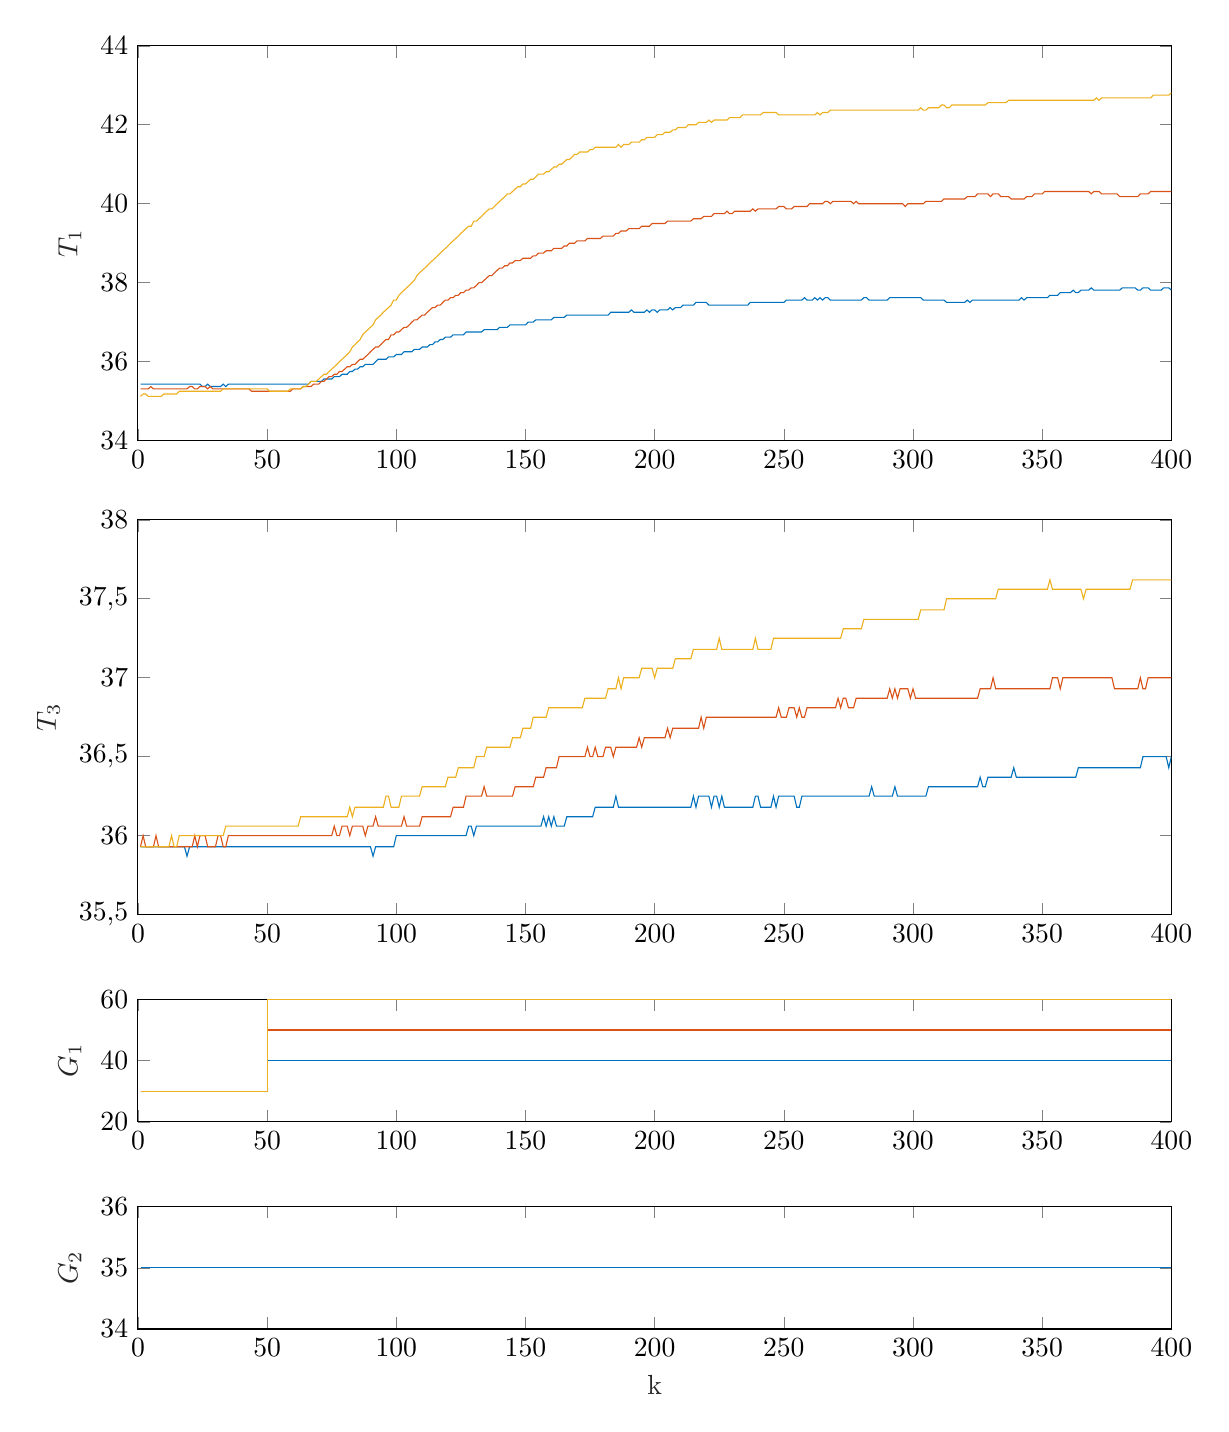
\begin{tikzpicture}

\begin{axis}[%
width=5.167in,
height=0.612in,
at={(0.646in,0.494in)},
scale only axis,
xmin=0,
xmax=400,
xtick={0,50,100,150,200,250,300,350,400},
xlabel style={font=\color{white!15!black}},
xlabel={k},
ymin=34,
ymax=36,
ytick={34,35,36},
ylabel style={font=\color{white!15!black}},
ylabel={$\text{G}_\text{2}$},
axis background/.style={fill=white}
]
\addplot[const plot, color=mycolor1, forget plot] table[row sep=crcr] {%
1	35\\
2	35\\
3	35\\
4	35\\
5	35\\
6	35\\
7	35\\
8	35\\
9	35\\
10	35\\
11	35\\
12	35\\
13	35\\
14	35\\
15	35\\
16	35\\
17	35\\
18	35\\
19	35\\
20	35\\
21	35\\
22	35\\
23	35\\
24	35\\
25	35\\
26	35\\
27	35\\
28	35\\
29	35\\
30	35\\
31	35\\
32	35\\
33	35\\
34	35\\
35	35\\
36	35\\
37	35\\
38	35\\
39	35\\
40	35\\
41	35\\
42	35\\
43	35\\
44	35\\
45	35\\
46	35\\
47	35\\
48	35\\
49	35\\
50	35\\
51	35\\
52	35\\
53	35\\
54	35\\
55	35\\
56	35\\
57	35\\
58	35\\
59	35\\
60	35\\
61	35\\
62	35\\
63	35\\
64	35\\
65	35\\
66	35\\
67	35\\
68	35\\
69	35\\
70	35\\
71	35\\
72	35\\
73	35\\
74	35\\
75	35\\
76	35\\
77	35\\
78	35\\
79	35\\
80	35\\
81	35\\
82	35\\
83	35\\
84	35\\
85	35\\
86	35\\
87	35\\
88	35\\
89	35\\
90	35\\
91	35\\
92	35\\
93	35\\
94	35\\
95	35\\
96	35\\
97	35\\
98	35\\
99	35\\
100	35\\
101	35\\
102	35\\
103	35\\
104	35\\
105	35\\
106	35\\
107	35\\
108	35\\
109	35\\
110	35\\
111	35\\
112	35\\
113	35\\
114	35\\
115	35\\
116	35\\
117	35\\
118	35\\
119	35\\
120	35\\
121	35\\
122	35\\
123	35\\
124	35\\
125	35\\
126	35\\
127	35\\
128	35\\
129	35\\
130	35\\
131	35\\
132	35\\
133	35\\
134	35\\
135	35\\
136	35\\
137	35\\
138	35\\
139	35\\
140	35\\
141	35\\
142	35\\
143	35\\
144	35\\
145	35\\
146	35\\
147	35\\
148	35\\
149	35\\
150	35\\
151	35\\
152	35\\
153	35\\
154	35\\
155	35\\
156	35\\
157	35\\
158	35\\
159	35\\
160	35\\
161	35\\
162	35\\
163	35\\
164	35\\
165	35\\
166	35\\
167	35\\
168	35\\
169	35\\
170	35\\
171	35\\
172	35\\
173	35\\
174	35\\
175	35\\
176	35\\
177	35\\
178	35\\
179	35\\
180	35\\
181	35\\
182	35\\
183	35\\
184	35\\
185	35\\
186	35\\
187	35\\
188	35\\
189	35\\
190	35\\
191	35\\
192	35\\
193	35\\
194	35\\
195	35\\
196	35\\
197	35\\
198	35\\
199	35\\
200	35\\
201	35\\
202	35\\
203	35\\
204	35\\
205	35\\
206	35\\
207	35\\
208	35\\
209	35\\
210	35\\
211	35\\
212	35\\
213	35\\
214	35\\
215	35\\
216	35\\
217	35\\
218	35\\
219	35\\
220	35\\
221	35\\
222	35\\
223	35\\
224	35\\
225	35\\
226	35\\
227	35\\
228	35\\
229	35\\
230	35\\
231	35\\
232	35\\
233	35\\
234	35\\
235	35\\
236	35\\
237	35\\
238	35\\
239	35\\
240	35\\
241	35\\
242	35\\
243	35\\
244	35\\
245	35\\
246	35\\
247	35\\
248	35\\
249	35\\
250	35\\
251	35\\
252	35\\
253	35\\
254	35\\
255	35\\
256	35\\
257	35\\
258	35\\
259	35\\
260	35\\
261	35\\
262	35\\
263	35\\
264	35\\
265	35\\
266	35\\
267	35\\
268	35\\
269	35\\
270	35\\
271	35\\
272	35\\
273	35\\
274	35\\
275	35\\
276	35\\
277	35\\
278	35\\
279	35\\
280	35\\
281	35\\
282	35\\
283	35\\
284	35\\
285	35\\
286	35\\
287	35\\
288	35\\
289	35\\
290	35\\
291	35\\
292	35\\
293	35\\
294	35\\
295	35\\
296	35\\
297	35\\
298	35\\
299	35\\
300	35\\
301	35\\
302	35\\
303	35\\
304	35\\
305	35\\
306	35\\
307	35\\
308	35\\
309	35\\
310	35\\
311	35\\
312	35\\
313	35\\
314	35\\
315	35\\
316	35\\
317	35\\
318	35\\
319	35\\
320	35\\
321	35\\
322	35\\
323	35\\
324	35\\
325	35\\
326	35\\
327	35\\
328	35\\
329	35\\
330	35\\
331	35\\
332	35\\
333	35\\
334	35\\
335	35\\
336	35\\
337	35\\
338	35\\
339	35\\
340	35\\
341	35\\
342	35\\
343	35\\
344	35\\
345	35\\
346	35\\
347	35\\
348	35\\
349	35\\
350	35\\
351	35\\
352	35\\
353	35\\
354	35\\
355	35\\
356	35\\
357	35\\
358	35\\
359	35\\
360	35\\
361	35\\
362	35\\
363	35\\
364	35\\
365	35\\
366	35\\
367	35\\
368	35\\
369	35\\
370	35\\
371	35\\
372	35\\
373	35\\
374	35\\
375	35\\
376	35\\
377	35\\
378	35\\
379	35\\
380	35\\
381	35\\
382	35\\
383	35\\
384	35\\
385	35\\
386	35\\
387	35\\
388	35\\
389	35\\
390	35\\
391	35\\
392	35\\
393	35\\
394	35\\
395	35\\
396	35\\
397	35\\
398	35\\
399	35\\
400	35\\
};
\end{axis}

\begin{axis}[%
width=5.167in,
height=0.612in,
at={(0.646in,1.53in)},
scale only axis,
xmin=0,
xmax=400,
xtick={0,50,100,150,200,250,300,350,400},
ymin=20,
ymax=60,
ytick={20,40,60},
ylabel style={font=\color{white!15!black}},
ylabel={$\text{G}_\text{1}$},
axis background/.style={fill=white}
]
\addplot[const plot, color=mycolor1, forget plot] table[row sep=crcr] {%
1	30\\
2	30\\
3	30\\
4	30\\
5	30\\
6	30\\
7	30\\
8	30\\
9	30\\
10	30\\
11	30\\
12	30\\
13	30\\
14	30\\
15	30\\
16	30\\
17	30\\
18	30\\
19	30\\
20	30\\
21	30\\
22	30\\
23	30\\
24	30\\
25	30\\
26	30\\
27	30\\
28	30\\
29	30\\
30	30\\
31	30\\
32	30\\
33	30\\
34	30\\
35	30\\
36	30\\
37	30\\
38	30\\
39	30\\
40	30\\
41	30\\
42	30\\
43	30\\
44	30\\
45	30\\
46	30\\
47	30\\
48	30\\
49	30\\
50	40\\
51	40\\
52	40\\
53	40\\
54	40\\
55	40\\
56	40\\
57	40\\
58	40\\
59	40\\
60	40\\
61	40\\
62	40\\
63	40\\
64	40\\
65	40\\
66	40\\
67	40\\
68	40\\
69	40\\
70	40\\
71	40\\
72	40\\
73	40\\
74	40\\
75	40\\
76	40\\
77	40\\
78	40\\
79	40\\
80	40\\
81	40\\
82	40\\
83	40\\
84	40\\
85	40\\
86	40\\
87	40\\
88	40\\
89	40\\
90	40\\
91	40\\
92	40\\
93	40\\
94	40\\
95	40\\
96	40\\
97	40\\
98	40\\
99	40\\
100	40\\
101	40\\
102	40\\
103	40\\
104	40\\
105	40\\
106	40\\
107	40\\
108	40\\
109	40\\
110	40\\
111	40\\
112	40\\
113	40\\
114	40\\
115	40\\
116	40\\
117	40\\
118	40\\
119	40\\
120	40\\
121	40\\
122	40\\
123	40\\
124	40\\
125	40\\
126	40\\
127	40\\
128	40\\
129	40\\
130	40\\
131	40\\
132	40\\
133	40\\
134	40\\
135	40\\
136	40\\
137	40\\
138	40\\
139	40\\
140	40\\
141	40\\
142	40\\
143	40\\
144	40\\
145	40\\
146	40\\
147	40\\
148	40\\
149	40\\
150	40\\
151	40\\
152	40\\
153	40\\
154	40\\
155	40\\
156	40\\
157	40\\
158	40\\
159	40\\
160	40\\
161	40\\
162	40\\
163	40\\
164	40\\
165	40\\
166	40\\
167	40\\
168	40\\
169	40\\
170	40\\
171	40\\
172	40\\
173	40\\
174	40\\
175	40\\
176	40\\
177	40\\
178	40\\
179	40\\
180	40\\
181	40\\
182	40\\
183	40\\
184	40\\
185	40\\
186	40\\
187	40\\
188	40\\
189	40\\
190	40\\
191	40\\
192	40\\
193	40\\
194	40\\
195	40\\
196	40\\
197	40\\
198	40\\
199	40\\
200	40\\
201	40\\
202	40\\
203	40\\
204	40\\
205	40\\
206	40\\
207	40\\
208	40\\
209	40\\
210	40\\
211	40\\
212	40\\
213	40\\
214	40\\
215	40\\
216	40\\
217	40\\
218	40\\
219	40\\
220	40\\
221	40\\
222	40\\
223	40\\
224	40\\
225	40\\
226	40\\
227	40\\
228	40\\
229	40\\
230	40\\
231	40\\
232	40\\
233	40\\
234	40\\
235	40\\
236	40\\
237	40\\
238	40\\
239	40\\
240	40\\
241	40\\
242	40\\
243	40\\
244	40\\
245	40\\
246	40\\
247	40\\
248	40\\
249	40\\
250	40\\
251	40\\
252	40\\
253	40\\
254	40\\
255	40\\
256	40\\
257	40\\
258	40\\
259	40\\
260	40\\
261	40\\
262	40\\
263	40\\
264	40\\
265	40\\
266	40\\
267	40\\
268	40\\
269	40\\
270	40\\
271	40\\
272	40\\
273	40\\
274	40\\
275	40\\
276	40\\
277	40\\
278	40\\
279	40\\
280	40\\
281	40\\
282	40\\
283	40\\
284	40\\
285	40\\
286	40\\
287	40\\
288	40\\
289	40\\
290	40\\
291	40\\
292	40\\
293	40\\
294	40\\
295	40\\
296	40\\
297	40\\
298	40\\
299	40\\
300	40\\
301	40\\
302	40\\
303	40\\
304	40\\
305	40\\
306	40\\
307	40\\
308	40\\
309	40\\
310	40\\
311	40\\
312	40\\
313	40\\
314	40\\
315	40\\
316	40\\
317	40\\
318	40\\
319	40\\
320	40\\
321	40\\
322	40\\
323	40\\
324	40\\
325	40\\
326	40\\
327	40\\
328	40\\
329	40\\
330	40\\
331	40\\
332	40\\
333	40\\
334	40\\
335	40\\
336	40\\
337	40\\
338	40\\
339	40\\
340	40\\
341	40\\
342	40\\
343	40\\
344	40\\
345	40\\
346	40\\
347	40\\
348	40\\
349	40\\
350	40\\
351	40\\
352	40\\
353	40\\
354	40\\
355	40\\
356	40\\
357	40\\
358	40\\
359	40\\
360	40\\
361	40\\
362	40\\
363	40\\
364	40\\
365	40\\
366	40\\
367	40\\
368	40\\
369	40\\
370	40\\
371	40\\
372	40\\
373	40\\
374	40\\
375	40\\
376	40\\
377	40\\
378	40\\
379	40\\
380	40\\
381	40\\
382	40\\
383	40\\
384	40\\
385	40\\
386	40\\
387	40\\
388	40\\
389	40\\
390	40\\
391	40\\
392	40\\
393	40\\
394	40\\
395	40\\
396	40\\
397	40\\
398	40\\
399	40\\
400	40\\
};
\addplot[const plot, color=mycolor2, forget plot] table[row sep=crcr] {%
1	30\\
2	30\\
3	30\\
4	30\\
5	30\\
6	30\\
7	30\\
8	30\\
9	30\\
10	30\\
11	30\\
12	30\\
13	30\\
14	30\\
15	30\\
16	30\\
17	30\\
18	30\\
19	30\\
20	30\\
21	30\\
22	30\\
23	30\\
24	30\\
25	30\\
26	30\\
27	30\\
28	30\\
29	30\\
30	30\\
31	30\\
32	30\\
33	30\\
34	30\\
35	30\\
36	30\\
37	30\\
38	30\\
39	30\\
40	30\\
41	30\\
42	30\\
43	30\\
44	30\\
45	30\\
46	30\\
47	30\\
48	30\\
49	30\\
50	50\\
51	50\\
52	50\\
53	50\\
54	50\\
55	50\\
56	50\\
57	50\\
58	50\\
59	50\\
60	50\\
61	50\\
62	50\\
63	50\\
64	50\\
65	50\\
66	50\\
67	50\\
68	50\\
69	50\\
70	50\\
71	50\\
72	50\\
73	50\\
74	50\\
75	50\\
76	50\\
77	50\\
78	50\\
79	50\\
80	50\\
81	50\\
82	50\\
83	50\\
84	50\\
85	50\\
86	50\\
87	50\\
88	50\\
89	50\\
90	50\\
91	50\\
92	50\\
93	50\\
94	50\\
95	50\\
96	50\\
97	50\\
98	50\\
99	50\\
100	50\\
101	50\\
102	50\\
103	50\\
104	50\\
105	50\\
106	50\\
107	50\\
108	50\\
109	50\\
110	50\\
111	50\\
112	50\\
113	50\\
114	50\\
115	50\\
116	50\\
117	50\\
118	50\\
119	50\\
120	50\\
121	50\\
122	50\\
123	50\\
124	50\\
125	50\\
126	50\\
127	50\\
128	50\\
129	50\\
130	50\\
131	50\\
132	50\\
133	50\\
134	50\\
135	50\\
136	50\\
137	50\\
138	50\\
139	50\\
140	50\\
141	50\\
142	50\\
143	50\\
144	50\\
145	50\\
146	50\\
147	50\\
148	50\\
149	50\\
150	50\\
151	50\\
152	50\\
153	50\\
154	50\\
155	50\\
156	50\\
157	50\\
158	50\\
159	50\\
160	50\\
161	50\\
162	50\\
163	50\\
164	50\\
165	50\\
166	50\\
167	50\\
168	50\\
169	50\\
170	50\\
171	50\\
172	50\\
173	50\\
174	50\\
175	50\\
176	50\\
177	50\\
178	50\\
179	50\\
180	50\\
181	50\\
182	50\\
183	50\\
184	50\\
185	50\\
186	50\\
187	50\\
188	50\\
189	50\\
190	50\\
191	50\\
192	50\\
193	50\\
194	50\\
195	50\\
196	50\\
197	50\\
198	50\\
199	50\\
200	50\\
201	50\\
202	50\\
203	50\\
204	50\\
205	50\\
206	50\\
207	50\\
208	50\\
209	50\\
210	50\\
211	50\\
212	50\\
213	50\\
214	50\\
215	50\\
216	50\\
217	50\\
218	50\\
219	50\\
220	50\\
221	50\\
222	50\\
223	50\\
224	50\\
225	50\\
226	50\\
227	50\\
228	50\\
229	50\\
230	50\\
231	50\\
232	50\\
233	50\\
234	50\\
235	50\\
236	50\\
237	50\\
238	50\\
239	50\\
240	50\\
241	50\\
242	50\\
243	50\\
244	50\\
245	50\\
246	50\\
247	50\\
248	50\\
249	50\\
250	50\\
251	50\\
252	50\\
253	50\\
254	50\\
255	50\\
256	50\\
257	50\\
258	50\\
259	50\\
260	50\\
261	50\\
262	50\\
263	50\\
264	50\\
265	50\\
266	50\\
267	50\\
268	50\\
269	50\\
270	50\\
271	50\\
272	50\\
273	50\\
274	50\\
275	50\\
276	50\\
277	50\\
278	50\\
279	50\\
280	50\\
281	50\\
282	50\\
283	50\\
284	50\\
285	50\\
286	50\\
287	50\\
288	50\\
289	50\\
290	50\\
291	50\\
292	50\\
293	50\\
294	50\\
295	50\\
296	50\\
297	50\\
298	50\\
299	50\\
300	50\\
301	50\\
302	50\\
303	50\\
304	50\\
305	50\\
306	50\\
307	50\\
308	50\\
309	50\\
310	50\\
311	50\\
312	50\\
313	50\\
314	50\\
315	50\\
316	50\\
317	50\\
318	50\\
319	50\\
320	50\\
321	50\\
322	50\\
323	50\\
324	50\\
325	50\\
326	50\\
327	50\\
328	50\\
329	50\\
330	50\\
331	50\\
332	50\\
333	50\\
334	50\\
335	50\\
336	50\\
337	50\\
338	50\\
339	50\\
340	50\\
341	50\\
342	50\\
343	50\\
344	50\\
345	50\\
346	50\\
347	50\\
348	50\\
349	50\\
350	50\\
351	50\\
352	50\\
353	50\\
354	50\\
355	50\\
356	50\\
357	50\\
358	50\\
359	50\\
360	50\\
361	50\\
362	50\\
363	50\\
364	50\\
365	50\\
366	50\\
367	50\\
368	50\\
369	50\\
370	50\\
371	50\\
372	50\\
373	50\\
374	50\\
375	50\\
376	50\\
377	50\\
378	50\\
379	50\\
380	50\\
381	50\\
382	50\\
383	50\\
384	50\\
385	50\\
386	50\\
387	50\\
388	50\\
389	50\\
390	50\\
391	50\\
392	50\\
393	50\\
394	50\\
395	50\\
396	50\\
397	50\\
398	50\\
399	50\\
400	50\\
};
\addplot[const plot, color=mycolor3, forget plot] table[row sep=crcr] {%
1	30\\
2	30\\
3	30\\
4	30\\
5	30\\
6	30\\
7	30\\
8	30\\
9	30\\
10	30\\
11	30\\
12	30\\
13	30\\
14	30\\
15	30\\
16	30\\
17	30\\
18	30\\
19	30\\
20	30\\
21	30\\
22	30\\
23	30\\
24	30\\
25	30\\
26	30\\
27	30\\
28	30\\
29	30\\
30	30\\
31	30\\
32	30\\
33	30\\
34	30\\
35	30\\
36	30\\
37	30\\
38	30\\
39	30\\
40	30\\
41	30\\
42	30\\
43	30\\
44	30\\
45	30\\
46	30\\
47	30\\
48	30\\
49	30\\
50	60\\
51	60\\
52	60\\
53	60\\
54	60\\
55	60\\
56	60\\
57	60\\
58	60\\
59	60\\
60	60\\
61	60\\
62	60\\
63	60\\
64	60\\
65	60\\
66	60\\
67	60\\
68	60\\
69	60\\
70	60\\
71	60\\
72	60\\
73	60\\
74	60\\
75	60\\
76	60\\
77	60\\
78	60\\
79	60\\
80	60\\
81	60\\
82	60\\
83	60\\
84	60\\
85	60\\
86	60\\
87	60\\
88	60\\
89	60\\
90	60\\
91	60\\
92	60\\
93	60\\
94	60\\
95	60\\
96	60\\
97	60\\
98	60\\
99	60\\
100	60\\
101	60\\
102	60\\
103	60\\
104	60\\
105	60\\
106	60\\
107	60\\
108	60\\
109	60\\
110	60\\
111	60\\
112	60\\
113	60\\
114	60\\
115	60\\
116	60\\
117	60\\
118	60\\
119	60\\
120	60\\
121	60\\
122	60\\
123	60\\
124	60\\
125	60\\
126	60\\
127	60\\
128	60\\
129	60\\
130	60\\
131	60\\
132	60\\
133	60\\
134	60\\
135	60\\
136	60\\
137	60\\
138	60\\
139	60\\
140	60\\
141	60\\
142	60\\
143	60\\
144	60\\
145	60\\
146	60\\
147	60\\
148	60\\
149	60\\
150	60\\
151	60\\
152	60\\
153	60\\
154	60\\
155	60\\
156	60\\
157	60\\
158	60\\
159	60\\
160	60\\
161	60\\
162	60\\
163	60\\
164	60\\
165	60\\
166	60\\
167	60\\
168	60\\
169	60\\
170	60\\
171	60\\
172	60\\
173	60\\
174	60\\
175	60\\
176	60\\
177	60\\
178	60\\
179	60\\
180	60\\
181	60\\
182	60\\
183	60\\
184	60\\
185	60\\
186	60\\
187	60\\
188	60\\
189	60\\
190	60\\
191	60\\
192	60\\
193	60\\
194	60\\
195	60\\
196	60\\
197	60\\
198	60\\
199	60\\
200	60\\
201	60\\
202	60\\
203	60\\
204	60\\
205	60\\
206	60\\
207	60\\
208	60\\
209	60\\
210	60\\
211	60\\
212	60\\
213	60\\
214	60\\
215	60\\
216	60\\
217	60\\
218	60\\
219	60\\
220	60\\
221	60\\
222	60\\
223	60\\
224	60\\
225	60\\
226	60\\
227	60\\
228	60\\
229	60\\
230	60\\
231	60\\
232	60\\
233	60\\
234	60\\
235	60\\
236	60\\
237	60\\
238	60\\
239	60\\
240	60\\
241	60\\
242	60\\
243	60\\
244	60\\
245	60\\
246	60\\
247	60\\
248	60\\
249	60\\
250	60\\
251	60\\
252	60\\
253	60\\
254	60\\
255	60\\
256	60\\
257	60\\
258	60\\
259	60\\
260	60\\
261	60\\
262	60\\
263	60\\
264	60\\
265	60\\
266	60\\
267	60\\
268	60\\
269	60\\
270	60\\
271	60\\
272	60\\
273	60\\
274	60\\
275	60\\
276	60\\
277	60\\
278	60\\
279	60\\
280	60\\
281	60\\
282	60\\
283	60\\
284	60\\
285	60\\
286	60\\
287	60\\
288	60\\
289	60\\
290	60\\
291	60\\
292	60\\
293	60\\
294	60\\
295	60\\
296	60\\
297	60\\
298	60\\
299	60\\
300	60\\
301	60\\
302	60\\
303	60\\
304	60\\
305	60\\
306	60\\
307	60\\
308	60\\
309	60\\
310	60\\
311	60\\
312	60\\
313	60\\
314	60\\
315	60\\
316	60\\
317	60\\
318	60\\
319	60\\
320	60\\
321	60\\
322	60\\
323	60\\
324	60\\
325	60\\
326	60\\
327	60\\
328	60\\
329	60\\
330	60\\
331	60\\
332	60\\
333	60\\
334	60\\
335	60\\
336	60\\
337	60\\
338	60\\
339	60\\
340	60\\
341	60\\
342	60\\
343	60\\
344	60\\
345	60\\
346	60\\
347	60\\
348	60\\
349	60\\
350	60\\
351	60\\
352	60\\
353	60\\
354	60\\
355	60\\
356	60\\
357	60\\
358	60\\
359	60\\
360	60\\
361	60\\
362	60\\
363	60\\
364	60\\
365	60\\
366	60\\
367	60\\
368	60\\
369	60\\
370	60\\
371	60\\
372	60\\
373	60\\
374	60\\
375	60\\
376	60\\
377	60\\
378	60\\
379	60\\
380	60\\
381	60\\
382	60\\
383	60\\
384	60\\
385	60\\
386	60\\
387	60\\
388	60\\
389	60\\
390	60\\
391	60\\
392	60\\
393	60\\
394	60\\
395	60\\
396	60\\
397	60\\
398	60\\
399	60\\
400	60\\
};
\end{axis}

\begin{axis}[%
width=5.167in,
height=1.974in,
at={(0.646in,2.566in)},
scale only axis,
xmin=0,
xmax=400,
xtick={0,50,100,150,200,250,300,350,400},
ymin=35.5,
ymax=38,
ytick={35.5,36,36.5,37,37.5,38},
yticklabels={{35,5},{36},{36,5},{37},{37,5},{38}},
ylabel style={font=\color{white!15!black}},
ylabel={$\text{T}_\text{3}$},
axis background/.style={fill=white}
]
\addplot [color=mycolor1, forget plot]
  table[row sep=crcr]{%
1	35.93\\
2	35.93\\
3	35.93\\
4	35.93\\
5	35.93\\
6	35.93\\
7	35.93\\
8	35.93\\
9	35.93\\
10	35.93\\
11	35.93\\
12	35.93\\
13	35.93\\
14	35.93\\
15	35.93\\
16	35.93\\
17	35.93\\
18	35.93\\
19	35.87\\
20	35.93\\
21	35.93\\
22	35.93\\
23	35.93\\
24	35.93\\
25	35.93\\
26	35.93\\
27	35.93\\
28	35.93\\
29	35.93\\
30	35.93\\
31	35.93\\
32	35.93\\
33	35.93\\
34	35.93\\
35	35.93\\
36	35.93\\
37	35.93\\
38	35.93\\
39	35.93\\
40	35.93\\
41	35.93\\
42	35.93\\
43	35.93\\
44	35.93\\
45	35.93\\
46	35.93\\
47	35.93\\
48	35.93\\
49	35.93\\
50	35.93\\
51	35.93\\
52	35.93\\
53	35.93\\
54	35.93\\
55	35.93\\
56	35.93\\
57	35.93\\
58	35.93\\
59	35.93\\
60	35.93\\
61	35.93\\
62	35.93\\
63	35.93\\
64	35.93\\
65	35.93\\
66	35.93\\
67	35.93\\
68	35.93\\
69	35.93\\
70	35.93\\
71	35.93\\
72	35.93\\
73	35.93\\
74	35.93\\
75	35.93\\
76	35.93\\
77	35.93\\
78	35.93\\
79	35.93\\
80	35.93\\
81	35.93\\
82	35.93\\
83	35.93\\
84	35.93\\
85	35.93\\
86	35.93\\
87	35.93\\
88	35.93\\
89	35.93\\
90	35.93\\
91	35.87\\
92	35.93\\
93	35.93\\
94	35.93\\
95	35.93\\
96	35.93\\
97	35.93\\
98	35.93\\
99	35.93\\
100	36\\
101	36\\
102	36\\
103	36\\
104	36\\
105	36\\
106	36\\
107	36\\
108	36\\
109	36\\
110	36\\
111	36\\
112	36\\
113	36\\
114	36\\
115	36\\
116	36\\
117	36\\
118	36\\
119	36\\
120	36\\
121	36\\
122	36\\
123	36\\
124	36\\
125	36\\
126	36\\
127	36\\
128	36.06\\
129	36.06\\
130	36\\
131	36.06\\
132	36.06\\
133	36.06\\
134	36.06\\
135	36.06\\
136	36.06\\
137	36.06\\
138	36.06\\
139	36.06\\
140	36.06\\
141	36.06\\
142	36.06\\
143	36.06\\
144	36.06\\
145	36.06\\
146	36.06\\
147	36.06\\
148	36.06\\
149	36.06\\
150	36.06\\
151	36.06\\
152	36.06\\
153	36.06\\
154	36.06\\
155	36.06\\
156	36.06\\
157	36.12\\
158	36.06\\
159	36.12\\
160	36.06\\
161	36.12\\
162	36.06\\
163	36.06\\
164	36.06\\
165	36.06\\
166	36.12\\
167	36.12\\
168	36.12\\
169	36.12\\
170	36.12\\
171	36.12\\
172	36.12\\
173	36.12\\
174	36.12\\
175	36.12\\
176	36.12\\
177	36.18\\
178	36.18\\
179	36.18\\
180	36.18\\
181	36.18\\
182	36.18\\
183	36.18\\
184	36.18\\
185	36.25\\
186	36.18\\
187	36.18\\
188	36.18\\
189	36.18\\
190	36.18\\
191	36.18\\
192	36.18\\
193	36.18\\
194	36.18\\
195	36.18\\
196	36.18\\
197	36.18\\
198	36.18\\
199	36.18\\
200	36.18\\
201	36.18\\
202	36.18\\
203	36.18\\
204	36.18\\
205	36.18\\
206	36.18\\
207	36.18\\
208	36.18\\
209	36.18\\
210	36.18\\
211	36.18\\
212	36.18\\
213	36.18\\
214	36.18\\
215	36.25\\
216	36.18\\
217	36.25\\
218	36.25\\
219	36.25\\
220	36.25\\
221	36.25\\
222	36.18\\
223	36.25\\
224	36.25\\
225	36.18\\
226	36.25\\
227	36.18\\
228	36.18\\
229	36.18\\
230	36.18\\
231	36.18\\
232	36.18\\
233	36.18\\
234	36.18\\
235	36.18\\
236	36.18\\
237	36.18\\
238	36.18\\
239	36.25\\
240	36.25\\
241	36.18\\
242	36.18\\
243	36.18\\
244	36.18\\
245	36.18\\
246	36.25\\
247	36.18\\
248	36.25\\
249	36.25\\
250	36.25\\
251	36.25\\
252	36.25\\
253	36.25\\
254	36.25\\
255	36.18\\
256	36.18\\
257	36.25\\
258	36.25\\
259	36.25\\
260	36.25\\
261	36.25\\
262	36.25\\
263	36.25\\
264	36.25\\
265	36.25\\
266	36.25\\
267	36.25\\
268	36.25\\
269	36.25\\
270	36.25\\
271	36.25\\
272	36.25\\
273	36.25\\
274	36.25\\
275	36.25\\
276	36.25\\
277	36.25\\
278	36.25\\
279	36.25\\
280	36.25\\
281	36.25\\
282	36.25\\
283	36.25\\
284	36.31\\
285	36.25\\
286	36.25\\
287	36.25\\
288	36.25\\
289	36.25\\
290	36.25\\
291	36.25\\
292	36.25\\
293	36.31\\
294	36.25\\
295	36.25\\
296	36.25\\
297	36.25\\
298	36.25\\
299	36.25\\
300	36.25\\
301	36.25\\
302	36.25\\
303	36.25\\
304	36.25\\
305	36.25\\
306	36.31\\
307	36.31\\
308	36.31\\
309	36.31\\
310	36.31\\
311	36.31\\
312	36.31\\
313	36.31\\
314	36.31\\
315	36.31\\
316	36.31\\
317	36.31\\
318	36.31\\
319	36.31\\
320	36.31\\
321	36.31\\
322	36.31\\
323	36.31\\
324	36.31\\
325	36.31\\
326	36.37\\
327	36.31\\
328	36.31\\
329	36.37\\
330	36.37\\
331	36.37\\
332	36.37\\
333	36.37\\
334	36.37\\
335	36.37\\
336	36.37\\
337	36.37\\
338	36.37\\
339	36.43\\
340	36.37\\
341	36.37\\
342	36.37\\
343	36.37\\
344	36.37\\
345	36.37\\
346	36.37\\
347	36.37\\
348	36.37\\
349	36.37\\
350	36.37\\
351	36.37\\
352	36.37\\
353	36.37\\
354	36.37\\
355	36.37\\
356	36.37\\
357	36.37\\
358	36.37\\
359	36.37\\
360	36.37\\
361	36.37\\
362	36.37\\
363	36.37\\
364	36.43\\
365	36.43\\
366	36.43\\
367	36.43\\
368	36.43\\
369	36.43\\
370	36.43\\
371	36.43\\
372	36.43\\
373	36.43\\
374	36.43\\
375	36.43\\
376	36.43\\
377	36.43\\
378	36.43\\
379	36.43\\
380	36.43\\
381	36.43\\
382	36.43\\
383	36.43\\
384	36.43\\
385	36.43\\
386	36.43\\
387	36.43\\
388	36.43\\
389	36.5\\
390	36.5\\
391	36.5\\
392	36.5\\
393	36.5\\
394	36.5\\
395	36.5\\
396	36.5\\
397	36.5\\
398	36.5\\
399	36.43\\
400	36.5\\
};
\addplot [color=mycolor2, forget plot]
  table[row sep=crcr]{%
1	35.93\\
2	36\\
3	35.93\\
4	35.93\\
5	35.93\\
6	35.93\\
7	36\\
8	35.93\\
9	35.93\\
10	35.93\\
11	35.93\\
12	35.93\\
13	35.93\\
14	35.93\\
15	35.93\\
16	35.93\\
17	35.93\\
18	35.93\\
19	35.93\\
20	35.93\\
21	35.93\\
22	36\\
23	35.93\\
24	36\\
25	36\\
26	36\\
27	35.93\\
28	35.93\\
29	35.93\\
30	35.93\\
31	36\\
32	36\\
33	35.93\\
34	35.93\\
35	36\\
36	36\\
37	36\\
38	36\\
39	36\\
40	36\\
41	36\\
42	36\\
43	36\\
44	36\\
45	36\\
46	36\\
47	36\\
48	36\\
49	36\\
50	36\\
51	36\\
52	36\\
53	36\\
54	36\\
55	36\\
56	36\\
57	36\\
58	36\\
59	36\\
60	36\\
61	36\\
62	36\\
63	36\\
64	36\\
65	36\\
66	36\\
67	36\\
68	36\\
69	36\\
70	36\\
71	36\\
72	36\\
73	36\\
74	36\\
75	36\\
76	36.06\\
77	36\\
78	36\\
79	36.06\\
80	36.06\\
81	36.06\\
82	36\\
83	36.06\\
84	36.06\\
85	36.06\\
86	36.06\\
87	36.06\\
88	36\\
89	36.06\\
90	36.06\\
91	36.06\\
92	36.12\\
93	36.06\\
94	36.06\\
95	36.06\\
96	36.06\\
97	36.06\\
98	36.06\\
99	36.06\\
100	36.06\\
101	36.06\\
102	36.06\\
103	36.12\\
104	36.06\\
105	36.06\\
106	36.06\\
107	36.06\\
108	36.06\\
109	36.06\\
110	36.12\\
111	36.12\\
112	36.12\\
113	36.12\\
114	36.12\\
115	36.12\\
116	36.12\\
117	36.12\\
118	36.12\\
119	36.12\\
120	36.12\\
121	36.12\\
122	36.18\\
123	36.18\\
124	36.18\\
125	36.18\\
126	36.18\\
127	36.25\\
128	36.25\\
129	36.25\\
130	36.25\\
131	36.25\\
132	36.25\\
133	36.25\\
134	36.31\\
135	36.25\\
136	36.25\\
137	36.25\\
138	36.25\\
139	36.25\\
140	36.25\\
141	36.25\\
142	36.25\\
143	36.25\\
144	36.25\\
145	36.25\\
146	36.31\\
147	36.31\\
148	36.31\\
149	36.31\\
150	36.31\\
151	36.31\\
152	36.31\\
153	36.31\\
154	36.37\\
155	36.37\\
156	36.37\\
157	36.37\\
158	36.43\\
159	36.43\\
160	36.43\\
161	36.43\\
162	36.43\\
163	36.5\\
164	36.5\\
165	36.5\\
166	36.5\\
167	36.5\\
168	36.5\\
169	36.5\\
170	36.5\\
171	36.5\\
172	36.5\\
173	36.5\\
174	36.56\\
175	36.5\\
176	36.5\\
177	36.56\\
178	36.5\\
179	36.5\\
180	36.5\\
181	36.56\\
182	36.56\\
183	36.56\\
184	36.5\\
185	36.56\\
186	36.56\\
187	36.56\\
188	36.56\\
189	36.56\\
190	36.56\\
191	36.56\\
192	36.56\\
193	36.56\\
194	36.62\\
195	36.56\\
196	36.62\\
197	36.62\\
198	36.62\\
199	36.62\\
200	36.62\\
201	36.62\\
202	36.62\\
203	36.62\\
204	36.62\\
205	36.68\\
206	36.62\\
207	36.68\\
208	36.68\\
209	36.68\\
210	36.68\\
211	36.68\\
212	36.68\\
213	36.68\\
214	36.68\\
215	36.68\\
216	36.68\\
217	36.68\\
218	36.75\\
219	36.68\\
220	36.75\\
221	36.75\\
222	36.75\\
223	36.75\\
224	36.75\\
225	36.75\\
226	36.75\\
227	36.75\\
228	36.75\\
229	36.75\\
230	36.75\\
231	36.75\\
232	36.75\\
233	36.75\\
234	36.75\\
235	36.75\\
236	36.75\\
237	36.75\\
238	36.75\\
239	36.75\\
240	36.75\\
241	36.75\\
242	36.75\\
243	36.75\\
244	36.75\\
245	36.75\\
246	36.75\\
247	36.75\\
248	36.81\\
249	36.75\\
250	36.75\\
251	36.75\\
252	36.81\\
253	36.81\\
254	36.81\\
255	36.75\\
256	36.81\\
257	36.75\\
258	36.75\\
259	36.81\\
260	36.81\\
261	36.81\\
262	36.81\\
263	36.81\\
264	36.81\\
265	36.81\\
266	36.81\\
267	36.81\\
268	36.81\\
269	36.81\\
270	36.81\\
271	36.87\\
272	36.81\\
273	36.87\\
274	36.87\\
275	36.81\\
276	36.81\\
277	36.81\\
278	36.87\\
279	36.87\\
280	36.87\\
281	36.87\\
282	36.87\\
283	36.87\\
284	36.87\\
285	36.87\\
286	36.87\\
287	36.87\\
288	36.87\\
289	36.87\\
290	36.87\\
291	36.93\\
292	36.87\\
293	36.93\\
294	36.87\\
295	36.93\\
296	36.93\\
297	36.93\\
298	36.93\\
299	36.87\\
300	36.93\\
301	36.87\\
302	36.87\\
303	36.87\\
304	36.87\\
305	36.87\\
306	36.87\\
307	36.87\\
308	36.87\\
309	36.87\\
310	36.87\\
311	36.87\\
312	36.87\\
313	36.87\\
314	36.87\\
315	36.87\\
316	36.87\\
317	36.87\\
318	36.87\\
319	36.87\\
320	36.87\\
321	36.87\\
322	36.87\\
323	36.87\\
324	36.87\\
325	36.87\\
326	36.93\\
327	36.93\\
328	36.93\\
329	36.93\\
330	36.93\\
331	37\\
332	36.93\\
333	36.93\\
334	36.93\\
335	36.93\\
336	36.93\\
337	36.93\\
338	36.93\\
339	36.93\\
340	36.93\\
341	36.93\\
342	36.93\\
343	36.93\\
344	36.93\\
345	36.93\\
346	36.93\\
347	36.93\\
348	36.93\\
349	36.93\\
350	36.93\\
351	36.93\\
352	36.93\\
353	36.93\\
354	37\\
355	37\\
356	37\\
357	36.93\\
358	37\\
359	37\\
360	37\\
361	37\\
362	37\\
363	37\\
364	37\\
365	37\\
366	37\\
367	37\\
368	37\\
369	37\\
370	37\\
371	37\\
372	37\\
373	37\\
374	37\\
375	37\\
376	37\\
377	37\\
378	36.93\\
379	36.93\\
380	36.93\\
381	36.93\\
382	36.93\\
383	36.93\\
384	36.93\\
385	36.93\\
386	36.93\\
387	36.93\\
388	37\\
389	36.93\\
390	36.93\\
391	37\\
392	37\\
393	37\\
394	37\\
395	37\\
396	37\\
397	37\\
398	37\\
399	37\\
400	37\\
};
\addplot [color=mycolor3, forget plot]
  table[row sep=crcr]{%
1	35.93\\
2	35.93\\
3	35.93\\
4	35.93\\
5	35.93\\
6	35.93\\
7	35.93\\
8	35.93\\
9	35.93\\
10	35.93\\
11	35.93\\
12	35.93\\
13	36\\
14	35.93\\
15	35.93\\
16	36\\
17	36\\
18	36\\
19	36\\
20	36\\
21	36\\
22	36\\
23	36\\
24	36\\
25	36\\
26	36\\
27	36\\
28	36\\
29	36\\
30	36\\
31	36\\
32	36\\
33	36\\
34	36.06\\
35	36.06\\
36	36.06\\
37	36.06\\
38	36.06\\
39	36.06\\
40	36.06\\
41	36.06\\
42	36.06\\
43	36.06\\
44	36.06\\
45	36.06\\
46	36.06\\
47	36.06\\
48	36.06\\
49	36.06\\
50	36.06\\
51	36.06\\
52	36.06\\
53	36.06\\
54	36.06\\
55	36.06\\
56	36.06\\
57	36.06\\
58	36.06\\
59	36.06\\
60	36.06\\
61	36.06\\
62	36.06\\
63	36.12\\
64	36.12\\
65	36.12\\
66	36.12\\
67	36.12\\
68	36.12\\
69	36.12\\
70	36.12\\
71	36.12\\
72	36.12\\
73	36.12\\
74	36.12\\
75	36.12\\
76	36.12\\
77	36.12\\
78	36.12\\
79	36.12\\
80	36.12\\
81	36.12\\
82	36.18\\
83	36.12\\
84	36.18\\
85	36.18\\
86	36.18\\
87	36.18\\
88	36.18\\
89	36.18\\
90	36.18\\
91	36.18\\
92	36.18\\
93	36.18\\
94	36.18\\
95	36.18\\
96	36.25\\
97	36.25\\
98	36.18\\
99	36.18\\
100	36.18\\
101	36.18\\
102	36.25\\
103	36.25\\
104	36.25\\
105	36.25\\
106	36.25\\
107	36.25\\
108	36.25\\
109	36.25\\
110	36.31\\
111	36.31\\
112	36.31\\
113	36.31\\
114	36.31\\
115	36.31\\
116	36.31\\
117	36.31\\
118	36.31\\
119	36.31\\
120	36.37\\
121	36.37\\
122	36.37\\
123	36.37\\
124	36.43\\
125	36.43\\
126	36.43\\
127	36.43\\
128	36.43\\
129	36.43\\
130	36.43\\
131	36.5\\
132	36.5\\
133	36.5\\
134	36.5\\
135	36.56\\
136	36.56\\
137	36.56\\
138	36.56\\
139	36.56\\
140	36.56\\
141	36.56\\
142	36.56\\
143	36.56\\
144	36.56\\
145	36.62\\
146	36.62\\
147	36.62\\
148	36.62\\
149	36.68\\
150	36.68\\
151	36.68\\
152	36.68\\
153	36.75\\
154	36.75\\
155	36.75\\
156	36.75\\
157	36.75\\
158	36.75\\
159	36.81\\
160	36.81\\
161	36.81\\
162	36.81\\
163	36.81\\
164	36.81\\
165	36.81\\
166	36.81\\
167	36.81\\
168	36.81\\
169	36.81\\
170	36.81\\
171	36.81\\
172	36.81\\
173	36.87\\
174	36.87\\
175	36.87\\
176	36.87\\
177	36.87\\
178	36.87\\
179	36.87\\
180	36.87\\
181	36.87\\
182	36.93\\
183	36.93\\
184	36.93\\
185	36.93\\
186	37\\
187	36.93\\
188	37\\
189	37\\
190	37\\
191	37\\
192	37\\
193	37\\
194	37\\
195	37.06\\
196	37.06\\
197	37.06\\
198	37.06\\
199	37.06\\
200	37\\
201	37.06\\
202	37.06\\
203	37.06\\
204	37.06\\
205	37.06\\
206	37.06\\
207	37.06\\
208	37.12\\
209	37.12\\
210	37.12\\
211	37.12\\
212	37.12\\
213	37.12\\
214	37.12\\
215	37.18\\
216	37.18\\
217	37.18\\
218	37.18\\
219	37.18\\
220	37.18\\
221	37.18\\
222	37.18\\
223	37.18\\
224	37.18\\
225	37.25\\
226	37.18\\
227	37.18\\
228	37.18\\
229	37.18\\
230	37.18\\
231	37.18\\
232	37.18\\
233	37.18\\
234	37.18\\
235	37.18\\
236	37.18\\
237	37.18\\
238	37.18\\
239	37.25\\
240	37.18\\
241	37.18\\
242	37.18\\
243	37.18\\
244	37.18\\
245	37.18\\
246	37.25\\
247	37.25\\
248	37.25\\
249	37.25\\
250	37.25\\
251	37.25\\
252	37.25\\
253	37.25\\
254	37.25\\
255	37.25\\
256	37.25\\
257	37.25\\
258	37.25\\
259	37.25\\
260	37.25\\
261	37.25\\
262	37.25\\
263	37.25\\
264	37.25\\
265	37.25\\
266	37.25\\
267	37.25\\
268	37.25\\
269	37.25\\
270	37.25\\
271	37.25\\
272	37.25\\
273	37.31\\
274	37.31\\
275	37.31\\
276	37.31\\
277	37.31\\
278	37.31\\
279	37.31\\
280	37.31\\
281	37.37\\
282	37.37\\
283	37.37\\
284	37.37\\
285	37.37\\
286	37.37\\
287	37.37\\
288	37.37\\
289	37.37\\
290	37.37\\
291	37.37\\
292	37.37\\
293	37.37\\
294	37.37\\
295	37.37\\
296	37.37\\
297	37.37\\
298	37.37\\
299	37.37\\
300	37.37\\
301	37.37\\
302	37.37\\
303	37.43\\
304	37.43\\
305	37.43\\
306	37.43\\
307	37.43\\
308	37.43\\
309	37.43\\
310	37.43\\
311	37.43\\
312	37.43\\
313	37.5\\
314	37.5\\
315	37.5\\
316	37.5\\
317	37.5\\
318	37.5\\
319	37.5\\
320	37.5\\
321	37.5\\
322	37.5\\
323	37.5\\
324	37.5\\
325	37.5\\
326	37.5\\
327	37.5\\
328	37.5\\
329	37.5\\
330	37.5\\
331	37.5\\
332	37.5\\
333	37.56\\
334	37.56\\
335	37.56\\
336	37.56\\
337	37.56\\
338	37.56\\
339	37.56\\
340	37.56\\
341	37.56\\
342	37.56\\
343	37.56\\
344	37.56\\
345	37.56\\
346	37.56\\
347	37.56\\
348	37.56\\
349	37.56\\
350	37.56\\
351	37.56\\
352	37.56\\
353	37.62\\
354	37.56\\
355	37.56\\
356	37.56\\
357	37.56\\
358	37.56\\
359	37.56\\
360	37.56\\
361	37.56\\
362	37.56\\
363	37.56\\
364	37.56\\
365	37.56\\
366	37.5\\
367	37.56\\
368	37.56\\
369	37.56\\
370	37.56\\
371	37.56\\
372	37.56\\
373	37.56\\
374	37.56\\
375	37.56\\
376	37.56\\
377	37.56\\
378	37.56\\
379	37.56\\
380	37.56\\
381	37.56\\
382	37.56\\
383	37.56\\
384	37.56\\
385	37.62\\
386	37.62\\
387	37.62\\
388	37.62\\
389	37.62\\
390	37.62\\
391	37.62\\
392	37.62\\
393	37.62\\
394	37.62\\
395	37.62\\
396	37.62\\
397	37.62\\
398	37.62\\
399	37.62\\
400	37.62\\
};
\end{axis}

\begin{axis}[%
width=5.167in,
height=1.974in,
at={(0.646in,4.936in)},
scale only axis,
xmin=0,
xmax=400,
xtick={0,50,100,150,200,250,300,350,400},
ymin=34,
ymax=44,
ytick={34,36,38,40,42,44},
ylabel style={font=\color{white!15!black}},
ylabel={$\text{T}_\text{1}$},
axis background/.style={fill=white}
]
\addplot [color=mycolor1, forget plot]
  table[row sep=crcr]{%
1	35.43\\
2	35.43\\
3	35.43\\
4	35.43\\
5	35.43\\
6	35.43\\
7	35.43\\
8	35.43\\
9	35.43\\
10	35.43\\
11	35.43\\
12	35.43\\
13	35.43\\
14	35.43\\
15	35.43\\
16	35.43\\
17	35.43\\
18	35.43\\
19	35.43\\
20	35.43\\
21	35.43\\
22	35.43\\
23	35.43\\
24	35.43\\
25	35.37\\
26	35.37\\
27	35.43\\
28	35.37\\
29	35.37\\
30	35.37\\
31	35.37\\
32	35.37\\
33	35.43\\
34	35.37\\
35	35.43\\
36	35.43\\
37	35.43\\
38	35.43\\
39	35.43\\
40	35.43\\
41	35.43\\
42	35.43\\
43	35.43\\
44	35.43\\
45	35.43\\
46	35.43\\
47	35.43\\
48	35.43\\
49	35.43\\
50	35.43\\
51	35.43\\
52	35.43\\
53	35.43\\
54	35.43\\
55	35.43\\
56	35.43\\
57	35.43\\
58	35.43\\
59	35.43\\
60	35.43\\
61	35.43\\
62	35.43\\
63	35.43\\
64	35.43\\
65	35.43\\
66	35.43\\
67	35.5\\
68	35.5\\
69	35.5\\
70	35.5\\
71	35.5\\
72	35.56\\
73	35.56\\
74	35.56\\
75	35.56\\
76	35.62\\
77	35.62\\
78	35.62\\
79	35.68\\
80	35.68\\
81	35.68\\
82	35.75\\
83	35.75\\
84	35.81\\
85	35.81\\
86	35.87\\
87	35.87\\
88	35.93\\
89	35.93\\
90	35.93\\
91	35.93\\
92	36\\
93	36.06\\
94	36.06\\
95	36.06\\
96	36.06\\
97	36.12\\
98	36.12\\
99	36.12\\
100	36.18\\
101	36.18\\
102	36.18\\
103	36.25\\
104	36.25\\
105	36.25\\
106	36.25\\
107	36.31\\
108	36.31\\
109	36.31\\
110	36.37\\
111	36.37\\
112	36.37\\
113	36.43\\
114	36.43\\
115	36.5\\
116	36.5\\
117	36.56\\
118	36.56\\
119	36.62\\
120	36.62\\
121	36.62\\
122	36.68\\
123	36.68\\
124	36.68\\
125	36.68\\
126	36.68\\
127	36.75\\
128	36.75\\
129	36.75\\
130	36.75\\
131	36.75\\
132	36.75\\
133	36.75\\
134	36.81\\
135	36.81\\
136	36.81\\
137	36.81\\
138	36.81\\
139	36.81\\
140	36.87\\
141	36.87\\
142	36.87\\
143	36.87\\
144	36.93\\
145	36.93\\
146	36.93\\
147	36.93\\
148	36.93\\
149	36.93\\
150	36.93\\
151	37\\
152	37\\
153	37\\
154	37.06\\
155	37.06\\
156	37.06\\
157	37.06\\
158	37.06\\
159	37.06\\
160	37.06\\
161	37.12\\
162	37.12\\
163	37.12\\
164	37.12\\
165	37.12\\
166	37.18\\
167	37.18\\
168	37.18\\
169	37.18\\
170	37.18\\
171	37.18\\
172	37.18\\
173	37.18\\
174	37.18\\
175	37.18\\
176	37.18\\
177	37.18\\
178	37.18\\
179	37.18\\
180	37.18\\
181	37.18\\
182	37.18\\
183	37.25\\
184	37.25\\
185	37.25\\
186	37.25\\
187	37.25\\
188	37.25\\
189	37.25\\
190	37.25\\
191	37.31\\
192	37.25\\
193	37.25\\
194	37.25\\
195	37.25\\
196	37.25\\
197	37.31\\
198	37.25\\
199	37.31\\
200	37.31\\
201	37.25\\
202	37.31\\
203	37.31\\
204	37.31\\
205	37.31\\
206	37.37\\
207	37.31\\
208	37.37\\
209	37.37\\
210	37.37\\
211	37.43\\
212	37.43\\
213	37.43\\
214	37.43\\
215	37.43\\
216	37.5\\
217	37.5\\
218	37.5\\
219	37.5\\
220	37.5\\
221	37.43\\
222	37.43\\
223	37.43\\
224	37.43\\
225	37.43\\
226	37.43\\
227	37.43\\
228	37.43\\
229	37.43\\
230	37.43\\
231	37.43\\
232	37.43\\
233	37.43\\
234	37.43\\
235	37.43\\
236	37.43\\
237	37.5\\
238	37.5\\
239	37.5\\
240	37.5\\
241	37.5\\
242	37.5\\
243	37.5\\
244	37.5\\
245	37.5\\
246	37.5\\
247	37.5\\
248	37.5\\
249	37.5\\
250	37.5\\
251	37.56\\
252	37.56\\
253	37.56\\
254	37.56\\
255	37.56\\
256	37.56\\
257	37.56\\
258	37.62\\
259	37.56\\
260	37.56\\
261	37.56\\
262	37.62\\
263	37.56\\
264	37.62\\
265	37.56\\
266	37.62\\
267	37.62\\
268	37.56\\
269	37.56\\
270	37.56\\
271	37.56\\
272	37.56\\
273	37.56\\
274	37.56\\
275	37.56\\
276	37.56\\
277	37.56\\
278	37.56\\
279	37.56\\
280	37.56\\
281	37.62\\
282	37.62\\
283	37.56\\
284	37.56\\
285	37.56\\
286	37.56\\
287	37.56\\
288	37.56\\
289	37.56\\
290	37.56\\
291	37.62\\
292	37.62\\
293	37.62\\
294	37.62\\
295	37.62\\
296	37.62\\
297	37.62\\
298	37.62\\
299	37.62\\
300	37.62\\
301	37.62\\
302	37.62\\
303	37.62\\
304	37.56\\
305	37.56\\
306	37.56\\
307	37.56\\
308	37.56\\
309	37.56\\
310	37.56\\
311	37.56\\
312	37.56\\
313	37.5\\
314	37.5\\
315	37.5\\
316	37.5\\
317	37.5\\
318	37.5\\
319	37.5\\
320	37.5\\
321	37.56\\
322	37.5\\
323	37.56\\
324	37.56\\
325	37.56\\
326	37.56\\
327	37.56\\
328	37.56\\
329	37.56\\
330	37.56\\
331	37.56\\
332	37.56\\
333	37.56\\
334	37.56\\
335	37.56\\
336	37.56\\
337	37.56\\
338	37.56\\
339	37.56\\
340	37.56\\
341	37.56\\
342	37.62\\
343	37.56\\
344	37.62\\
345	37.62\\
346	37.62\\
347	37.62\\
348	37.62\\
349	37.62\\
350	37.62\\
351	37.62\\
352	37.62\\
353	37.68\\
354	37.68\\
355	37.68\\
356	37.68\\
357	37.75\\
358	37.75\\
359	37.75\\
360	37.75\\
361	37.75\\
362	37.81\\
363	37.75\\
364	37.75\\
365	37.81\\
366	37.81\\
367	37.81\\
368	37.81\\
369	37.87\\
370	37.81\\
371	37.81\\
372	37.81\\
373	37.81\\
374	37.81\\
375	37.81\\
376	37.81\\
377	37.81\\
378	37.81\\
379	37.81\\
380	37.81\\
381	37.87\\
382	37.87\\
383	37.87\\
384	37.87\\
385	37.87\\
386	37.87\\
387	37.81\\
388	37.81\\
389	37.87\\
390	37.87\\
391	37.87\\
392	37.81\\
393	37.81\\
394	37.81\\
395	37.81\\
396	37.81\\
397	37.87\\
398	37.87\\
399	37.87\\
400	37.81\\
};
\addplot [color=mycolor2, forget plot]
  table[row sep=crcr]{%
1	35.31\\
2	35.31\\
3	35.31\\
4	35.31\\
5	35.37\\
6	35.31\\
7	35.31\\
8	35.31\\
9	35.31\\
10	35.31\\
11	35.31\\
12	35.31\\
13	35.31\\
14	35.31\\
15	35.31\\
16	35.31\\
17	35.31\\
18	35.31\\
19	35.31\\
20	35.37\\
21	35.37\\
22	35.31\\
23	35.31\\
24	35.37\\
25	35.37\\
26	35.37\\
27	35.31\\
28	35.37\\
29	35.31\\
30	35.31\\
31	35.31\\
32	35.31\\
33	35.31\\
34	35.31\\
35	35.31\\
36	35.31\\
37	35.31\\
38	35.31\\
39	35.31\\
40	35.31\\
41	35.31\\
42	35.31\\
43	35.31\\
44	35.25\\
45	35.25\\
46	35.25\\
47	35.25\\
48	35.25\\
49	35.25\\
50	35.25\\
51	35.25\\
52	35.25\\
53	35.25\\
54	35.25\\
55	35.25\\
56	35.25\\
57	35.25\\
58	35.25\\
59	35.25\\
60	35.31\\
61	35.31\\
62	35.31\\
63	35.31\\
64	35.37\\
65	35.37\\
66	35.37\\
67	35.37\\
68	35.43\\
69	35.43\\
70	35.43\\
71	35.5\\
72	35.5\\
73	35.56\\
74	35.62\\
75	35.62\\
76	35.68\\
77	35.68\\
78	35.75\\
79	35.75\\
80	35.81\\
81	35.87\\
82	35.87\\
83	35.93\\
84	35.93\\
85	36\\
86	36.06\\
87	36.06\\
88	36.12\\
89	36.18\\
90	36.25\\
91	36.31\\
92	36.37\\
93	36.37\\
94	36.43\\
95	36.5\\
96	36.56\\
97	36.56\\
98	36.68\\
99	36.68\\
100	36.75\\
101	36.75\\
102	36.81\\
103	36.87\\
104	36.87\\
105	36.93\\
106	37\\
107	37.06\\
108	37.06\\
109	37.12\\
110	37.18\\
111	37.18\\
112	37.25\\
113	37.31\\
114	37.37\\
115	37.37\\
116	37.43\\
117	37.43\\
118	37.5\\
119	37.56\\
120	37.56\\
121	37.62\\
122	37.62\\
123	37.68\\
124	37.68\\
125	37.75\\
126	37.75\\
127	37.81\\
128	37.81\\
129	37.87\\
130	37.87\\
131	37.93\\
132	38\\
133	38\\
134	38.06\\
135	38.12\\
136	38.18\\
137	38.18\\
138	38.25\\
139	38.31\\
140	38.37\\
141	38.37\\
142	38.43\\
143	38.43\\
144	38.5\\
145	38.5\\
146	38.56\\
147	38.56\\
148	38.56\\
149	38.62\\
150	38.62\\
151	38.62\\
152	38.62\\
153	38.68\\
154	38.68\\
155	38.75\\
156	38.75\\
157	38.75\\
158	38.81\\
159	38.81\\
160	38.81\\
161	38.87\\
162	38.87\\
163	38.87\\
164	38.87\\
165	38.93\\
166	38.93\\
167	39\\
168	39\\
169	39\\
170	39.06\\
171	39.06\\
172	39.06\\
173	39.06\\
174	39.12\\
175	39.12\\
176	39.12\\
177	39.12\\
178	39.12\\
179	39.12\\
180	39.18\\
181	39.18\\
182	39.18\\
183	39.18\\
184	39.18\\
185	39.25\\
186	39.25\\
187	39.31\\
188	39.31\\
189	39.31\\
190	39.37\\
191	39.37\\
192	39.37\\
193	39.37\\
194	39.37\\
195	39.43\\
196	39.43\\
197	39.43\\
198	39.43\\
199	39.5\\
200	39.5\\
201	39.5\\
202	39.5\\
203	39.5\\
204	39.5\\
205	39.56\\
206	39.56\\
207	39.56\\
208	39.56\\
209	39.56\\
210	39.56\\
211	39.56\\
212	39.56\\
213	39.56\\
214	39.56\\
215	39.62\\
216	39.62\\
217	39.62\\
218	39.62\\
219	39.68\\
220	39.68\\
221	39.68\\
222	39.68\\
223	39.75\\
224	39.75\\
225	39.75\\
226	39.75\\
227	39.75\\
228	39.81\\
229	39.75\\
230	39.75\\
231	39.81\\
232	39.81\\
233	39.81\\
234	39.81\\
235	39.81\\
236	39.81\\
237	39.81\\
238	39.87\\
239	39.81\\
240	39.87\\
241	39.87\\
242	39.87\\
243	39.87\\
244	39.87\\
245	39.87\\
246	39.87\\
247	39.87\\
248	39.93\\
249	39.93\\
250	39.93\\
251	39.87\\
252	39.87\\
253	39.87\\
254	39.93\\
255	39.93\\
256	39.93\\
257	39.93\\
258	39.93\\
259	39.93\\
260	40\\
261	40\\
262	40\\
263	40\\
264	40\\
265	40\\
266	40.06\\
267	40.06\\
268	40\\
269	40.06\\
270	40.06\\
271	40.06\\
272	40.06\\
273	40.06\\
274	40.06\\
275	40.06\\
276	40.06\\
277	40\\
278	40.06\\
279	40\\
280	40\\
281	40\\
282	40\\
283	40\\
284	40\\
285	40\\
286	40\\
287	40\\
288	40\\
289	40\\
290	40\\
291	40\\
292	40\\
293	40\\
294	40\\
295	40\\
296	40\\
297	39.93\\
298	40\\
299	40\\
300	40\\
301	40\\
302	40\\
303	40\\
304	40\\
305	40.06\\
306	40.06\\
307	40.06\\
308	40.06\\
309	40.06\\
310	40.06\\
311	40.06\\
312	40.12\\
313	40.12\\
314	40.12\\
315	40.12\\
316	40.12\\
317	40.12\\
318	40.12\\
319	40.12\\
320	40.12\\
321	40.18\\
322	40.18\\
323	40.18\\
324	40.18\\
325	40.25\\
326	40.25\\
327	40.25\\
328	40.25\\
329	40.25\\
330	40.18\\
331	40.25\\
332	40.25\\
333	40.25\\
334	40.18\\
335	40.18\\
336	40.18\\
337	40.18\\
338	40.12\\
339	40.12\\
340	40.12\\
341	40.12\\
342	40.12\\
343	40.12\\
344	40.18\\
345	40.18\\
346	40.18\\
347	40.25\\
348	40.25\\
349	40.25\\
350	40.25\\
351	40.31\\
352	40.31\\
353	40.31\\
354	40.31\\
355	40.31\\
356	40.31\\
357	40.31\\
358	40.31\\
359	40.31\\
360	40.31\\
361	40.31\\
362	40.31\\
363	40.31\\
364	40.31\\
365	40.31\\
366	40.31\\
367	40.31\\
368	40.31\\
369	40.25\\
370	40.31\\
371	40.31\\
372	40.31\\
373	40.25\\
374	40.25\\
375	40.25\\
376	40.25\\
377	40.25\\
378	40.25\\
379	40.25\\
380	40.18\\
381	40.18\\
382	40.18\\
383	40.18\\
384	40.18\\
385	40.18\\
386	40.18\\
387	40.18\\
388	40.25\\
389	40.25\\
390	40.25\\
391	40.25\\
392	40.31\\
393	40.31\\
394	40.31\\
395	40.31\\
396	40.31\\
397	40.31\\
398	40.31\\
399	40.31\\
400	40.31\\
};
\addplot [color=mycolor3, forget plot]
  table[row sep=crcr]{%
1	35.12\\
2	35.18\\
3	35.18\\
4	35.12\\
5	35.12\\
6	35.12\\
7	35.12\\
8	35.12\\
9	35.12\\
10	35.18\\
11	35.18\\
12	35.18\\
13	35.18\\
14	35.18\\
15	35.18\\
16	35.25\\
17	35.25\\
18	35.25\\
19	35.25\\
20	35.25\\
21	35.25\\
22	35.25\\
23	35.25\\
24	35.25\\
25	35.25\\
26	35.25\\
27	35.25\\
28	35.25\\
29	35.25\\
30	35.25\\
31	35.25\\
32	35.25\\
33	35.31\\
34	35.31\\
35	35.31\\
36	35.31\\
37	35.31\\
38	35.31\\
39	35.31\\
40	35.31\\
41	35.31\\
42	35.31\\
43	35.31\\
44	35.31\\
45	35.31\\
46	35.31\\
47	35.31\\
48	35.31\\
49	35.31\\
50	35.31\\
51	35.25\\
52	35.25\\
53	35.25\\
54	35.25\\
55	35.25\\
56	35.25\\
57	35.25\\
58	35.25\\
59	35.31\\
60	35.31\\
61	35.31\\
62	35.31\\
63	35.31\\
64	35.37\\
65	35.37\\
66	35.43\\
67	35.5\\
68	35.5\\
69	35.5\\
70	35.56\\
71	35.62\\
72	35.68\\
73	35.68\\
74	35.75\\
75	35.81\\
76	35.87\\
77	35.93\\
78	36\\
79	36.06\\
80	36.12\\
81	36.18\\
82	36.25\\
83	36.37\\
84	36.43\\
85	36.5\\
86	36.56\\
87	36.68\\
88	36.75\\
89	36.81\\
90	36.87\\
91	36.93\\
92	37.06\\
93	37.12\\
94	37.18\\
95	37.25\\
96	37.31\\
97	37.37\\
98	37.43\\
99	37.56\\
100	37.56\\
101	37.68\\
102	37.75\\
103	37.81\\
104	37.87\\
105	37.93\\
106	38\\
107	38.06\\
108	38.18\\
109	38.25\\
110	38.31\\
111	38.37\\
112	38.43\\
113	38.5\\
114	38.56\\
115	38.62\\
116	38.68\\
117	38.75\\
118	38.81\\
119	38.87\\
120	38.93\\
121	39\\
122	39.06\\
123	39.12\\
124	39.18\\
125	39.25\\
126	39.31\\
127	39.37\\
128	39.43\\
129	39.43\\
130	39.56\\
131	39.56\\
132	39.62\\
133	39.68\\
134	39.75\\
135	39.81\\
136	39.87\\
137	39.87\\
138	39.93\\
139	40\\
140	40.06\\
141	40.12\\
142	40.18\\
143	40.25\\
144	40.25\\
145	40.31\\
146	40.37\\
147	40.43\\
148	40.43\\
149	40.5\\
150	40.5\\
151	40.56\\
152	40.62\\
153	40.62\\
154	40.68\\
155	40.75\\
156	40.75\\
157	40.75\\
158	40.81\\
159	40.81\\
160	40.87\\
161	40.93\\
162	40.93\\
163	41\\
164	41\\
165	41.06\\
166	41.12\\
167	41.12\\
168	41.18\\
169	41.25\\
170	41.25\\
171	41.31\\
172	41.31\\
173	41.31\\
174	41.31\\
175	41.37\\
176	41.37\\
177	41.43\\
178	41.43\\
179	41.43\\
180	41.43\\
181	41.43\\
182	41.43\\
183	41.43\\
184	41.43\\
185	41.43\\
186	41.5\\
187	41.43\\
188	41.5\\
189	41.5\\
190	41.5\\
191	41.56\\
192	41.56\\
193	41.56\\
194	41.56\\
195	41.62\\
196	41.62\\
197	41.68\\
198	41.68\\
199	41.68\\
200	41.68\\
201	41.75\\
202	41.75\\
203	41.75\\
204	41.81\\
205	41.81\\
206	41.81\\
207	41.87\\
208	41.87\\
209	41.93\\
210	41.93\\
211	41.93\\
212	41.93\\
213	42\\
214	42\\
215	42\\
216	42\\
217	42.06\\
218	42.06\\
219	42.06\\
220	42.06\\
221	42.12\\
222	42.06\\
223	42.12\\
224	42.12\\
225	42.12\\
226	42.12\\
227	42.12\\
228	42.12\\
229	42.18\\
230	42.18\\
231	42.18\\
232	42.18\\
233	42.18\\
234	42.25\\
235	42.25\\
236	42.25\\
237	42.25\\
238	42.25\\
239	42.25\\
240	42.25\\
241	42.25\\
242	42.31\\
243	42.31\\
244	42.31\\
245	42.31\\
246	42.31\\
247	42.31\\
248	42.25\\
249	42.25\\
250	42.25\\
251	42.25\\
252	42.25\\
253	42.25\\
254	42.25\\
255	42.25\\
256	42.25\\
257	42.25\\
258	42.25\\
259	42.25\\
260	42.25\\
261	42.25\\
262	42.25\\
263	42.31\\
264	42.25\\
265	42.31\\
266	42.31\\
267	42.31\\
268	42.37\\
269	42.37\\
270	42.37\\
271	42.37\\
272	42.37\\
273	42.37\\
274	42.37\\
275	42.37\\
276	42.37\\
277	42.37\\
278	42.37\\
279	42.37\\
280	42.37\\
281	42.37\\
282	42.37\\
283	42.37\\
284	42.37\\
285	42.37\\
286	42.37\\
287	42.37\\
288	42.37\\
289	42.37\\
290	42.37\\
291	42.37\\
292	42.37\\
293	42.37\\
294	42.37\\
295	42.37\\
296	42.37\\
297	42.37\\
298	42.37\\
299	42.37\\
300	42.37\\
301	42.37\\
302	42.37\\
303	42.43\\
304	42.37\\
305	42.37\\
306	42.43\\
307	42.43\\
308	42.43\\
309	42.43\\
310	42.43\\
311	42.5\\
312	42.5\\
313	42.43\\
314	42.43\\
315	42.5\\
316	42.5\\
317	42.5\\
318	42.5\\
319	42.5\\
320	42.5\\
321	42.5\\
322	42.5\\
323	42.5\\
324	42.5\\
325	42.5\\
326	42.5\\
327	42.5\\
328	42.5\\
329	42.56\\
330	42.56\\
331	42.56\\
332	42.56\\
333	42.56\\
334	42.56\\
335	42.56\\
336	42.56\\
337	42.62\\
338	42.62\\
339	42.62\\
340	42.62\\
341	42.62\\
342	42.62\\
343	42.62\\
344	42.62\\
345	42.62\\
346	42.62\\
347	42.62\\
348	42.62\\
349	42.62\\
350	42.62\\
351	42.62\\
352	42.62\\
353	42.62\\
354	42.62\\
355	42.62\\
356	42.62\\
357	42.62\\
358	42.62\\
359	42.62\\
360	42.62\\
361	42.62\\
362	42.62\\
363	42.62\\
364	42.62\\
365	42.62\\
366	42.62\\
367	42.62\\
368	42.62\\
369	42.62\\
370	42.62\\
371	42.68\\
372	42.62\\
373	42.68\\
374	42.68\\
375	42.68\\
376	42.68\\
377	42.68\\
378	42.68\\
379	42.68\\
380	42.68\\
381	42.68\\
382	42.68\\
383	42.68\\
384	42.68\\
385	42.68\\
386	42.68\\
387	42.68\\
388	42.68\\
389	42.68\\
390	42.68\\
391	42.68\\
392	42.68\\
393	42.75\\
394	42.75\\
395	42.75\\
396	42.75\\
397	42.75\\
398	42.75\\
399	42.75\\
400	42.81\\
};
\end{axis}
\end{tikzpicture}%
\caption{Odpowiedzi modelu na różne skoki sygnału sterowania z punktu pracy} 
\label{Z2steps}
\end{figure}

Symulując odpowiedź układu dla różnych wartości skoku sygnału sterującego otrzymujemy charakterystykę statyczną widoczną na rys. \ref{Z2stat}.

\begin{figure}[ht]
\centering
% This file was created by matlab2tikz.
%
%The latest updates can be retrieved from
%  http://www.mathworks.com/matlabcentral/fileexchange/22022-matlab2tikz-matlab2tikz
%where you can also make suggestions and rate matlab2tikz.
%
\definecolor{mycolor1}{rgb}{0.00000,0.44700,0.74100}%
%
\begin{tikzpicture}

\begin{axis}[%
width=4.521in,
height=3.566in,
at={(0.758in,0.481in)},
scale only axis,
xmin=-1,
xmax=1,
xtick={-1,-0.8,-0.6,-0.4,-0.2,0,0.2,0.4,0.6,0.8,1},
xticklabels={{-1},{-0,8},{-0,6},{-0,4},{-0,2},{0},{0,2},{0,4},{0,6},{0,8},{1}},
xlabel style={font=\color{white!15!black}},
xlabel={u},
ymin=-1,
ymax=8,
ytick={-1,0,1,2,3,4,5,6,7,8},
ylabel style={font=\color{white!15!black}},
ylabel={$y$},
axis background/.style={fill=white}
]
\addplot [color=mycolor1, forget plot]
  table[row sep=crcr]{%
-1	-0.214603120511242\\
-0.98	-0.212734311981145\\
-0.96	-0.210876252677139\\
-0.94	-0.209028076514733\\
-0.92	-0.207189029895327\\
-0.9	-0.205358475831417\\
-0.88	-0.203535896388567\\
-0.86	-0.201720892978527\\
-0.84	-0.199913183953989\\
-0.82	-0.198112598859099\\
-0.8	-0.196319068579716\\
-0.78	-0.194532610511869\\
-0.76	-0.192753307724504\\
-0.74	-0.190981280931843\\
-0.72	-0.189216651910009\\
-0.7	-0.187459496790879\\
-0.68	-0.185709787442253\\
-0.66	-0.183967318896933\\
-0.64	-0.18223162052433\\
-0.62	-0.180501848347764\\
-0.6	-0.178776655600994\\
-0.58	-0.177054038292739\\
-0.56	-0.175331152214082\\
-0.54	-0.173604097489592\\
-0.52	-0.171867666451075\\
-0.5	-0.170115050319639\\
-0.48	-0.168337499938879\\
-0.46	-0.166523935637207\\
-0.44	-0.16466050124546\\
-0.42	-0.162730057399575\\
-0.4	-0.160711609568663\\
-0.38	-0.158579666826696\\
-0.36	-0.156303528300488\\
-0.34	-0.153846495555031\\
-0.32	-0.151165011002592\\
-0.3	-0.14820772482952\\
-0.28	-0.144914496006171\\
-0.26	-0.141215336750611\\
-0.24	-0.137029314403215\\
-0.22	-0.132263430047496\\
-0.2	-0.126811499339427\\
-0.18	-0.120553067767147\\
-0.16	-0.113352399745653\\
-0.14	-0.105057588234085\\
-0.12	-0.0954998384950576\\
-0.1	-0.0844929856087093\\
-0.08	-0.0718333096910282\\
-0.0599999999999999	-0.0572997146235803\\
-0.04	-0.0406543346000139\\
-0.02	-0.0216436270725326\\
0	0\\
0.02	0.0245559948322395\\
0.04	0.052312892336765\\
0.0600000000000001	0.0835649852353769\\
0.0800000000000001	0.118608483433522\\
0.1	0.157737242676167\\
0.12	0.201238176930391\\
0.14	0.249386499643944\\
0.16	0.302440963964915\\
0.18	0.360639288229532\\
0.2	0.424193958074067\\
0.22	0.493288588812914\\
0.24	0.568075010835338\\
0.26	0.648671207643992\\
0.28	0.735160193060859\\
0.3	0.827589864458871\\
0.32	0.925973816780111\\
0.34	1.03029305195621\\
0.36	1.14049847424278\\
0.38	1.25651402723634\\
0.4	1.37824030515851\\
0.42	1.50555846027741\\
0.44	1.63833422972876\\
0.46	1.77642191705088\\
0.48	1.91966818422543\\
0.5	2.06791553625701\\
0.52	2.22100540958487\\
0.54	2.37878080537289\\
0.56	2.54108843686578\\
0.58	2.70778038497171\\
0.6	2.8787152770487\\
0.62	3.05375902008132\\
0.64	3.23278513103008\\
0.66	3.41567471444857\\
0.68	3.60231614104717\\
0.7	3.79260448140675\\
0.72	3.98644074721583\\
0.74	4.18373098889018\\
0.76	4.38438529383471\\
0.78	4.58831672442457\\
0.8	4.79544022941308\\
0.82	5.00567155721645\\
0.84	5.21892619458407\\
0.86	5.43511834966648\\
0.88	5.65415999451122\\
0.9	5.87595997856422\\
0.92	6.10042322182181\\
0.94	6.32744999382564\\
0.96	6.55693528267039\\
0.98	6.78876825654486\\
1	7.02283181899276\\
};
\end{axis}
\end{tikzpicture}%
\caption{Wyznaczona charakterystyka statyczna modelu}
\label{Z2stat}
\end{figure}

Z otrzymanych wykresów można zauważyć, że właściwości statyczne i dynamiczne otrzymanego obiektu zdecydowanie nie są liniowe. Na wszystkich torach jest to układ dynamicznie samostabilizujący się, a jego opóźnienie dla poszczególnych torów zgadzają się z opóźneniami podanymi w definicji modelu w treści zadania. Czas stabilizacji różni się jednak w zależności od wartości skoku.


\chapter{Podpunkt 3}
Symulację cyfrowych algorytmów PID oraz DMC przeprowadzono korzystając odpowiednio ze skryptów \verb|PIDfuzzy.m| oraz \verb|DMCfuzzy.m| przy ustawieniu parametru ilości regulatorów jako 1. Dokładniejsze opisy implementacji zostaną przytoczone w podpunktach 5 oraz 6, gdzie wykorzystywane są wszystkie funkcje wymienionych wyżej skryptów.


\chapter{Podpunkt 4}
Ponieważ metoda eksperymentalnie była ekstensywnie wykorzystywana i opisywana w poprzednich projektach, poszczególne kroki dostrajania parametrów zwyczajnych algorytmów PID i DMC zostaną pominięte - przedstawione będą jedynie końcowe rezultaty.

W przypadku algorytmu PID wstępne parametry regulatora uzyskano korzystając z optymalizatora zawartego w skrypcie \verb|pid_params.m|. Następnie parametry te ręcznie modyfikowano dla uzyskania gładszego przebiegu funkcji w większej ilości okresów między skokami. Ostateczny wykres przedstawiono na rysunku \ref{Z4pid} - parametry w nim wykorzystane to $ K = \num{0,17} $, $ T_\mathrm{i} = \num{3,70} $ oraz $ T_\mathrm{d} = \num{1,07} $. 

\begin{figure}[ht]
	\centering
	% This file was created by matlab2tikz.
%
%The latest updates can be retrieved from
%  http://www.mathworks.com/matlabcentral/fileexchange/22022-matlab2tikz-matlab2tikz
%where you can also make suggestions and rate matlab2tikz.
%
ERR 1633.1
\definecolor{mycolor1}{rgb}{0.00000,0.44700,0.74100}%
\definecolor{mycolor2}{rgb}{0.85000,0.32500,0.09800}%
%
\begin{tikzpicture}

\begin{axis}[%
width=6.833in,
height=0.656in,
at={(0.854in,0.525in)},
scale only axis,
xmin=0,
xmax=1000,
xtick={0,100,200,300,400,500,600,700,800,900,1000},
xlabel style={font=\color{white!15!black}},
xlabel={k},
ymin=-1,
ymax=1,
ytick={-1,0,1},
ylabel style={font=\color{white!15!black}},
ylabel={u},
axis background/.style={fill=white}
]
\addplot[const plot, color=mycolor1, forget plot] table[row sep=crcr] {%
1	0\\
2	0\\
3	0\\
4	0\\
5	0\\
6	0\\
7	0\\
8	0\\
9	0\\
10	0\\
11	0\\
12	0\\
13	0\\
14	0\\
15	0\\
16	0\\
17	0\\
18	0\\
19	0\\
20	0\\
21	1\\
22	-1\\
23	-0.830865009230476\\
24	-0.661730018460952\\
25	-0.492595027691428\\
26	-0.430979410719595\\
27	-0.166886398838361\\
28	0.0448925850374864\\
29	0.21875363656965\\
30	0.387155678460691\\
31	0.554351901150181\\
32	0.72778711774849\\
33	0.888434062778946\\
34	1\\
35	1\\
36	1\\
37	1\\
38	1\\
39	1\\
40	1\\
41	1\\
42	1\\
43	1\\
44	1\\
45	1\\
46	1\\
47	1\\
48	1\\
49	1\\
50	1\\
51	1\\
52	1\\
53	1\\
54	1\\
55	1\\
56	1\\
57	1\\
58	1\\
59	1\\
60	1\\
61	1\\
62	1\\
63	1\\
64	1\\
65	1\\
66	1\\
67	1\\
68	1\\
69	1\\
70	1\\
71	1\\
72	1\\
73	1\\
74	0.999958603150014\\
75	0.999854360470655\\
76	0.999695012111869\\
77	0.999487344971364\\
78	0.99923731008164\\
79	0.998960016623465\\
80	0.99867730772647\\
81	0.998408523321295\\
82	0.998169191653349\\
83	0.997972269179217\\
84	0.997826530985312\\
85	0.997734734729294\\
86	0.997694278881645\\
87	0.997698667275022\\
88	0.99773844566798\\
89	0.997802249981098\\
90	0.997878311968663\\
91	0.997955826134795\\
92	0.99802584016365\\
93	0.998081826676195\\
94	0.998120003940935\\
95	0.998139307431096\\
96	0.998141030953359\\
97	0.998128275144916\\
98	0.998105305763507\\
99	0.998076880604587\\
100	0.998047619193676\\
101	0.998021490905889\\
102	0.998001461582326\\
103	0.997989307542011\\
104	0.997985591890556\\
105	0.99798978395524\\
106	0.998000486437189\\
107	0.998015726760212\\
108	0.998033270031907\\
109	0.998050915538248\\
110	0.998066745443461\\
111	0.998079304257357\\
112	0.998087699085742\\
113	0.998091621207787\\
114	0.99809129814185\\
115	0.998087391842282\\
116	0.998080862537046\\
117	0.998072818704385\\
118	0.998064372163114\\
119	0.998056513866238\\
120	0.998050021369842\\
121	0.998045403753914\\
122	0.998042884687023\\
123	0.998042419930077\\
124	0.998043742248092\\
125	0.998046424648816\\
126	0.998049952141539\\
127	0.998053792698705\\
128	0.998057459569786\\
129	0.998060559229463\\
130	0.998062821703422\\
131	0.998064112479797\\
132	0.998064427403198\\
133	0.998063873655256\\
134	0.998062641030183\\
135	0.998060968181195\\
136	0.998059108385268\\
137	0.998057298752707\\
138	0.998055735837158\\
139	0.998054559442509\\
140	0.998053845233576\\
141	0.998053605676185\\
142	0.998053797964659\\
143	0.99805433700692\\
144	0.998055111254003\\
145	0.998055999168637\\
146	0.998056884382537\\
147	0.998057668028934\\
148	0.998058277279462\\
149	0.998058669685927\\
150	0.998058833459298\\
151	0.99805878425621\\
152	0.998058559352117\\
153	0.998058210244266\\
154	0.998057794749889\\
155	0.998057369563991\\
156	0.998056984046428\\
157	0.998056675755524\\
158	0.998056467972179\\
159	0.998056369198156\\
160	0.998056374392389\\
161	0.998056467548508\\
162	0.998056625124544\\
163	0.998056819812368\\
164	0.998057024172089\\
165	0.998057213742246\\
166	0.998057369353332\\
167	0.99805747850229\\
168	0.998057535772432\\
169	0.998057542393068\\
170	0.998057505115953\\
171	0.998057434636397\\
172	0.998057343804324\\
173	0.998057245857874\\
174	0.998057152875117\\
175	0.998057074585898\\
176	0.998057017624209\\
177	0.998056985239989\\
178	0.998056977434691\\
179	0.998056991442551\\
180	0.998057022452099\\
181	0.998057064451089\\
182	0.998057111081386\\
183	0.998057156406092\\
184	0.998057195515538\\
185	0.998057224927779\\
186	0.998057242768982\\
187	0.998057248746001\\
188	0.998057243945043\\
189	0.998057230504872\\
190	0.99805721121994\\
191	0.99805718912853\\
192	0.998057167134499\\
193	0.998057147700226\\
194	0.998057132634798\\
195	0.998057122987155\\
196	0.99805711904066\\
197	0.998057120394691\\
198	0.998057126111147\\
199	0.998057134899752\\
200	0.998057145315561\\
201	-1\\
202	1\\
203	0.826032588589389\\
204	0.65206517465697\\
205	0.478097757997266\\
206	1\\
207	0.826748186528483\\
208	0.561774438261732\\
209	0.402790589364134\\
210	0.328040366984943\\
211	0.170621996245752\\
212	0.0149444744246265\\
213	-0.0515062951874037\\
214	-0.0511355570458047\\
215	-0.0316150595873861\\
216	0.0320584114977065\\
217	0.119421725214534\\
218	0.167695434332887\\
219	0.176005970854055\\
220	0.165693927071056\\
221	0.146312276387642\\
222	0.119677513235956\\
223	0.0902072832543755\\
224	0.0647870068943169\\
225	0.0462079924049879\\
226	0.0340242857438322\\
227	0.0271851699911799\\
228	0.0241926977085202\\
229	0.0228634279072942\\
230	0.0213399172174231\\
231	0.018747416928434\\
232	0.0149440749551955\\
233	0.0101362262156215\\
234	0.00469335602712173\\
235	-0.000974226078929469\\
236	-0.00653739278806248\\
237	-0.0118062513140215\\
238	-0.0167153616978059\\
239	-0.0212837125495527\\
240	-0.0255767228930295\\
241	-0.0296732733573939\\
242	-0.0336413520763899\\
243	-0.0375268737721644\\
244	-0.0413537065457226\\
245	-0.0451291827542993\\
246	-0.0488508631438198\\
247	-0.0525125132694333\\
248	-0.0561082780013114\\
249	-0.0596347612746938\\
250	-0.0630914238674527\\
251	-0.0664800204156016\\
252	-0.0698036932409284\\
253	-0.0730661123355348\\
254	-0.0762708570998236\\
255	-0.0794210876653865\\
256	-0.0825194543519562\\
257	-0.0855681537180864\\
258	-0.0885690461970856\\
259	-0.0915237767986174\\
260	-0.0944338682121916\\
261	-0.0973007775448908\\
262	-0.100125921633999\\
263	-0.102910681588298\\
264	-0.105656397163629\\
265	-0.10836435872571\\
266	-0.111035801141426\\
267	-0.113671901141162\\
268	-0.116273777915965\\
269	-0.11884249591182\\
270	-0.121379068680384\\
271	-0.123884462906849\\
272	-0.12635960209918\\
273	-0.128805369737731\\
274	-0.131222611891727\\
275	-0.13361213940936\\
276	-0.135974729810119\\
277	-0.138311128986504\\
278	-0.140622052786175\\
279	-0.142908188512057\\
280	-0.145170196354402\\
281	-0.147408710756161\\
282	-0.149624341708519\\
283	-0.151817675973917\\
284	-0.153989278236231\\
285	-0.156139692180309\\
286	-0.158269441504837\\
287	-0.160379030873352\\
288	-0.162468946808357\\
289	-0.16453965853313\\
290	-0.166591618765322\\
291	-0.168625264465912\\
292	-0.170641017546598\\
293	-0.172639285538409\\
294	-0.174620462223999\\
295	-0.176584928235922\\
296	-0.178533051623021\\
297	-0.180465188386897\\
298	-0.182381682990331\\
299	-0.184282868839375\\
300	-0.186169068740738\\
301	-0.188040595335958\\
302	-0.189897751513761\\
303	-0.191740830801903\\
304	-0.193570117739704\\
305	-0.195385888232404\\
306	-0.19718840988838\\
307	-0.198977942340217\\
308	-0.200754737550536\\
309	-0.20251904010344\\
310	-0.204271087482384\\
311	-0.206011110335201\\
312	-0.207739332727006\\
313	-0.209455972381619\\
314	-0.211161240912127\\
315	-0.212855344041176\\
316	-0.214538481811508\\
317	-0.216210848787289\\
318	-0.217872634246667\\
319	-0.219524022366048\\
320	-0.221165192396482\\
321	-0.222796318832581\\
322	-0.22441757157433\\
323	-0.22602911608215\\
324	-0.227631113525547\\
325	-0.229223720925661\\
326	-0.230807091292005\\
327	-0.232381373753687\\
328	-0.233946713685368\\
329	-0.23550325282821\\
330	-0.237051129406051\\
331	-0.238590478237031\\
332	-0.240121430840871\\
333	-0.241644115542023\\
334	-0.243158657568863\\
335	-0.244665179149114\\
336	-0.24616379960167\\
337	-0.247654635424975\\
338	-0.249137800382125\\
339	-0.250613405582817\\
340	-0.252081559562299\\
341	-0.253542368357445\\
342	-0.25499593558008\\
343	-0.256442362487674\\
344	-0.257881748051513\\
345	-0.259314189022462\\
346	-0.26073977999441\\
347	-0.262158613465501\\
348	-0.263570779897248\\
349	-0.264976367771598\\
350	-0.266375463646053\\
351	-0.267768152206916\\
352	-0.269154516320737\\
353	-0.270534637084032\\
354	-0.271908593871345\\
355	-0.273276464381721\\
356	-0.274638324683647\\
357	-0.275994249258523\\
358	-0.27734431104272\\
359	-0.278688581468283\\
360	-0.280027130502326\\
361	-0.28136002668517\\
362	-0.282687337167275\\
363	-0.284009127745003\\
364	-0.285325462895268\\
365	-0.286636405809103\\
366	-0.287942018424194\\
367	-0.289242361456404\\
368	-0.290537494430348\\
369	-0.291827475709023\\
370	-0.293112362522553\\
371	-0.294392210996073\\
372	-0.295667076176768\\
373	-0.296937012060125\\
374	-0.298202071615397\\
375	-0.299462306810329\\
376	-0.300717768635156\\
377	-0.301968507125908\\
378	-0.303214571387043\\
379	-0.30445600961343\\
380	-0.305692869111702\\
381	-0.306925196321004\\
382	-0.308153036833163\\
383	-0.309376435412276\\
384	-0.310595436013771\\
385	-0.311810081802917\\
386	-0.313020415172842\\
387	-0.314226477762045\\
388	-0.315428310471432\\
389	-0.316625953480886\\
390	-0.317819446265396\\
391	-0.319008827610747\\
392	-0.320194135628788\\
393	-0.321375407772297\\
394	-0.32255268084945\\
395	-0.323725991037914\\
396	-0.32489537389856\\
397	-0.326060864388827\\
398	-0.327222496875734\\
399	-0.328380305148561\\
400	-0.329534322431195\\
401	0.934106065412754\\
402	0.141764677218058\\
403	0.193778550422579\\
404	0.245796087139475\\
405	0.297817256797275\\
406	0.274415005031586\\
407	0.272748870500057\\
408	0.328412092313532\\
409	0.365506344554517\\
410	0.390090086825528\\
411	0.418141991675902\\
412	0.449817966744431\\
413	0.471579568225819\\
414	0.484916772372257\\
415	0.494771793100387\\
416	0.501160325824524\\
417	0.502784315416615\\
418	0.501251415957335\\
419	0.498638880281234\\
420	0.495600605492924\\
421	0.492447590913952\\
422	0.489904771935506\\
423	0.488486424621287\\
424	0.488166004602806\\
425	0.488737849087118\\
426	0.49001226984686\\
427	0.491706884533215\\
428	0.493456135780552\\
429	0.494954778879123\\
430	0.496012489012736\\
431	0.496525863573103\\
432	0.49647405278564\\
433	0.495926713569246\\
434	0.495019253249965\\
435	0.493913075195693\\
436	0.49276900751491\\
437	0.491729365727737\\
438	0.490900392197538\\
439	0.490341248963115\\
440	0.490064190217729\\
441	0.490041777441789\\
442	0.490217157915637\\
443	0.49051676033668\\
444	0.490863931162715\\
445	0.491190620818977\\
446	0.491445420742824\\
447	0.491597792359143\\
448	0.491638662785481\\
449	0.491577762943398\\
450	0.491438659473343\\
451	0.491252726062343\\
452	0.491053123483376\\
453	0.490869598656391\\
454	0.490724700590391\\
455	0.490631726134682\\
456	0.490594379527762\\
457	0.49060788011538\\
458	0.490661106438278\\
459	0.49073928970146\\
460	0.490826766874369\\
461	0.490909379772422\\
462	0.490976234623586\\
463	0.491020680570584\\
464	0.491040503033784\\
465	0.491037443272795\\
466	0.491016234291286\\
467	0.490983378861219\\
468	0.490945891644649\\
469	0.490910192854547\\
470	0.490881285750349\\
471	0.490862285789027\\
472	0.490854306563203\\
473	0.490856655474477\\
474	0.490867255845504\\
475	0.490883194224296\\
476	0.49090129146251\\
477	0.490918610706485\\
478	0.490932839999906\\
479	0.490942516425955\\
480	0.490947087553146\\
481	0.490946830264081\\
482	0.490942664102919\\
483	0.490935904904173\\
484	0.490928004934015\\
485	0.490920319483516\\
486	0.49091392891952\\
487	0.490909532029812\\
488	0.490907413390812\\
489	0.490907476314382\\
490	0.490909324960548\\
491	0.490912375017216\\
492	0.490915971880537\\
493	0.490919497929544\\
494	0.490922455337125\\
495	0.490924516806511\\
496	0.490925542612604\\
497	0.490925567485763\\
498	0.490924764604136\\
499	0.49092339597469\\
500	0.490921758797393\\
501	0.490920136279093\\
502	0.490918759213618\\
503	0.490917781964912\\
504	0.490917273761966\\
505	0.490917223840356\\
506	0.490917557225087\\
507	0.490918156981978\\
508	0.490918888572217\\
509	0.490919622417222\\
510	0.49092025173199\\
511	0.490920703892076\\
512	0.490920944842409\\
513	0.490920977149044\\
514	0.490920833106554\\
515	0.490920564776799\\
516	0.490920232944404\\
517	0.490919896777508\\
518	0.490919605562199\\
519	0.490919393335924\\
520	0.490919276679481\\
521	0.4909192554246\\
522	0.490919315656127\\
523	0.490919434166708\\
524	0.490919583461862\\
525	0.490919736494275\\
526	0.490919870491381\\
527	0.490919969484465\\
528	0.490920025404844\\
529	0.490920037843656\\
530	0.490920012747715\\
531	0.49091996042916\\
532	0.490919893298546\\
533	0.490919823698126\\
534	0.490919762130563\\
535	0.490919716068629\\
536	0.490919689414508\\
537	0.490919682571248\\
538	0.490919693007105\\
539	0.490919716143555\\
540	0.490919746381051\\
541	0.490919778089821\\
542	0.490919806428746\\
543	0.490919827904586\\
544	0.49091984063696\\
545	0.49091984434312\\
546	0.490919840094595\\
547	0.490919829921444\\
548	0.490919816348417\\
549	0.490919801942162\\
550	0.490919788932935\\
551	0.49091977895222\\
552	0.490919772903544\\
553	0.490919770961461\\
554	0.490919772676041\\
555	0.490919777149006\\
556	0.490919783243301\\
557	0.490919789789882\\
558	0.490919795762333\\
559	0.4909198003998\\
560	0.490919803269691\\
561	0.490919804271772\\
562	0.490919803593527\\
563	0.490919801631875\\
564	0.490919798898558\\
565	0.490919795925771\\
566	0.490919793185623\\
567	0.490919791032616\\
568	0.490919789673343\\
569	0.490919789162956\\
570	0.49091978942414\\
571	0.490919790281854\\
572	0.490919791506009\\
573	0.490919792854509\\
574	0.490919794110369\\
575	0.490919795108594\\
576	0.490919795750778\\
577	0.490919796007468\\
578	0.490919795910155\\
579	0.490919795535877\\
580	0.490919794987988\\
581	0.490919794376539\\
582	0.490919793801185\\
583	0.490919793338636\\
584	0.490919793035654\\
585	0.490919792907627\\
586	0.490919792941924\\
587	0.490919793104709\\
588	0.490919793349599\\
589	0.490919793626601\\
590	0.490919793889978\\
591	0.490919794104098\\
592	0.490919794246786\\
593	0.490919794310134\\
594	0.490919794299106\\
595	0.490919794228528\\
596	0.490919794119194\\
597	0.490919793993798\\
598	0.490919793873315\\
599	0.490919793774282\\
600	0.490919793707191\\
601	1\\
602	0.208805144580448\\
603	0.261961855995649\\
604	0.315118567429113\\
605	0.368275278870547\\
606	0.326370265478746\\
607	0.464702231438282\\
608	0.604863400127637\\
609	0.699681005907588\\
610	0.769608975104178\\
611	0.847156459738358\\
612	0.895613316885394\\
613	0.912104655591614\\
614	0.910228181097451\\
615	0.898150341261111\\
616	0.874732190607893\\
617	0.842883081996333\\
618	0.809185209966921\\
619	0.777752336143751\\
620	0.750212466197444\\
621	0.728316996526153\\
622	0.713823229080229\\
623	0.707102712476682\\
624	0.707293878546789\\
625	0.713085598999025\\
626	0.722821785947036\\
627	0.734446450762949\\
628	0.745900168790691\\
629	0.755554285705999\\
630	0.762331301966401\\
631	0.765696766858243\\
632	0.765659610843966\\
633	0.762697269143975\\
634	0.757592181637896\\
635	0.751267608792058\\
636	0.744660066525311\\
637	0.738610088149406\\
638	0.733771585901051\\
639	0.730558001007573\\
640	0.729127691703621\\
641	0.729399094584172\\
642	0.731090840899935\\
643	0.733783369570415\\
644	0.736992120167814\\
645	0.740239410444594\\
646	0.743115043262539\\
647	0.745319176856109\\
648	0.746683859441306\\
649	0.747173408017503\\
650	0.746867460292863\\
651	0.745932305247534\\
652	0.744586252473241\\
653	0.743064312982978\\
654	0.741586585708979\\
655	0.740333485253725\\
656	0.739429592523414\\
657	0.738936700564943\\
658	0.738855565135631\\
659	0.739134942191872\\
660	0.739685797210973\\
661	0.740398196796601\\
662	0.741158365407933\\
663	0.741863690999351\\
664	0.742434036628404\\
665	0.742818449995564\\
666	0.742997118311717\\
667	0.742979068917751\\
668	0.742796588358554\\
669	0.742497591592753\\
670	0.742137225517748\\
671	0.741769872729606\\
672	0.741442482239029\\
673	0.741189845014252\\
674	0.741032100431845\\
675	0.740974445142323\\
676	0.741008750798582\\
677	0.741116604778921\\
678	0.741273181657839\\
679	0.741451335089997\\
680	0.741625361336549\\
681	0.741774008681284\\
682	0.741882466940101\\
683	0.741943241635733\\
684	0.741955973965774\\
685	0.741926391891143\\
686	0.741864658503975\\
687	0.74178341804073\\
688	0.741695830905079\\
689	0.7416138451408\\
690	0.74154688407907\\
691	0.741501050473687\\
692	0.741478867831458\\
693	0.741479509564808\\
694	0.741499413179295\\
695	0.741533144075961\\
696	0.741574362708448\\
697	0.741616757963504\\
698	0.741654834654321\\
699	0.7416844784099\\
700	0.741703260960376\\
701	0.741710487149768\\
702	0.741707017292469\\
703	0.741694921566857\\
704	0.741677035522987\\
705	0.741656487579154\\
706	0.741636262019425\\
707	0.741618846826251\\
708	0.741605997512805\\
709	0.741598628836639\\
710	0.741596828451531\\
711	0.74159997218713\\
712	0.741606911004665\\
713	0.741616195252024\\
714	0.741626302398975\\
715	0.741635839150042\\
716	0.741643696486022\\
717	0.741649145366963\\
718	0.741651870151319\\
719	0.741651945053614\\
720	0.741649765297559\\
721	0.74164594852326\\
722	0.741641223359254\\
723	0.741636321094294\\
724	0.741631883559554\\
725	0.741628396296357\\
726	0.741626151528448\\
727	0.741625241031321\\
728	0.741625575228605\\
729	0.741626922117021\\
730	0.741628958111303\\
731	0.741631322612409\\
732	0.741633668886284\\
733	0.741635705434705\\
734	0.741637224120759\\
735	0.741638113543745\\
736	0.741638358238505\\
737	0.741638025964575\\
738	0.741637246498394\\
739	0.741636185886166\\
740	0.74163502007981\\
741	0.741633911356622\\
742	0.741632990054851\\
743	0.741632343103994\\
744	0.741632009750727\\
745	0.741631983917723\\
746	0.741632221886767\\
747	0.741632653529579\\
748	0.741633195136074\\
749	0.741633761987217\\
750	0.741634279134546\\
751	0.741634689308232\\
752	0.741634957400264\\
753	0.741635071483509\\
754	0.741635040767788\\
755	0.741634891217085\\
756	0.741634659734738\\
757	0.741634387864571\\
758	0.741634115871905\\
759	0.741633877888747\\
760	0.741633698569574\\
761	0.741633591446438\\
762	0.741633558930208\\
763	0.741633593706436\\
764	0.74163368113781\\
765	0.741633802218175\\
766	0.741633936623417\\
767	0.741634065461761\\
768	0.741634173424446\\
769	0.741634250158614\\
770	0.741634290808982\\
771	0.741634295787288\\
772	0.741634269916367\\
773	0.741634221151682\\
774	0.7416341591052\\
775	0.741634093586903\\
776	0.7416340333442\\
777	0.741633985127082\\
778	0.741633953146564\\
779	0.741633938934239\\
780	0.741633941559349\\
781	0.741633958121526\\
782	0.741633984415318\\
783	0.741634015656925\\
784	0.741634047172494\\
785	0.741634074967523\\
786	0.741634096124111\\
787	0.741634109002519\\
788	0.741634113251643\\
789	0.741634109656275\\
790	0.74163409986522\\
791	0.741634086052566\\
792	0.741634070564794\\
793	0.741634055600169\\
794	0.741634042955657\\
795	0.74163403386284\\
796	0.741634028919779\\
797	0.74163402811275\\
798	0.741634030911388\\
799	0.741634036414095\\
800	0.741634043517805\\
801	-1\\
802	0.330645900224964\\
803	0.241245982197078\\
804	0.151846062315002\\
805	0.0624461403839822\\
806	0.718804551516012\\
807	0.709275363942962\\
808	0.629079677803677\\
809	0.602269383516407\\
810	0.606918294250939\\
811	0.522717619727107\\
812	0.403550648429438\\
813	0.31925322770941\\
814	0.256799917604476\\
815	0.199258758931556\\
816	0.161415378219779\\
817	0.158861515369606\\
818	0.180255838493289\\
819	0.211145938950683\\
820	0.245624778077933\\
821	0.275730437781655\\
822	0.29336966986612\\
823	0.298117298428176\\
824	0.293470621588059\\
825	0.282398889427047\\
826	0.267488187515632\\
827	0.251825091222064\\
828	0.238127280375596\\
829	0.22792042879394\\
830	0.221743218989103\\
831	0.219472090554258\\
832	0.220347092728377\\
833	0.223151079088941\\
834	0.226625151027503\\
835	0.229775928348461\\
836	0.231970343406921\\
837	0.232937850431036\\
838	0.232725473990149\\
839	0.2315975448302\\
840	0.229916560380983\\
841	0.228048786637752\\
842	0.226301516050037\\
843	0.224884854580477\\
844	0.22389858627315\\
845	0.223343436646351\\
846	0.223147911007878\\
847	0.223200458366815\\
848	0.223380121929816\\
849	0.223580916285\\
850	0.223726731614648\\
851	0.22377634751186\\
852	0.223720610271326\\
853	0.223574684079447\\
854	0.223368152169493\\
855	0.223135336367969\\
856	0.222907543558531\\
857	0.222708088966391\\
858	0.222550179669482\\
859	0.222437225292268\\
860	0.222364846201\\
861	0.222323741004186\\
862	0.222302647302799\\
863	0.222290830442607\\
864	0.222279782354497\\
865	0.222264044872496\\
866	0.22224125510437\\
867	0.222211625203723\\
868	0.222177111366553\\
869	0.222140510032307\\
870	0.222104664483299\\
871	0.222071893188721\\
872	0.222043679667207\\
873	0.222020605139622\\
874	0.222002466797564\\
875	0.221988507308663\\
876	0.221977682218586\\
877	0.221968905880314\\
878	0.221961237305346\\
879	0.221953989192647\\
880	0.221946762060272\\
881	0.221939418413695\\
882	0.221932018495202\\
883	0.221924739991957\\
884	0.221917800628922\\
885	0.221911396682881\\
886	0.221905663884623\\
887	0.221900661306072\\
888	0.221896374518325\\
889	0.221892731890803\\
890	0.221889627278712\\
891	0.221886943118887\\
892	0.221884569586562\\
893	0.221882417418739\\
894	0.221880423839683\\
895	0.221878552435177\\
896	0.221876788678586\\
897	0.221875133116781\\
898	0.221873594079134\\
899	0.221872181332318\\
900	0.221870901531208\\
901	0.221869755752597\\
902	0.221868738943132\\
903	0.221867840817226\\
904	0.221867047612709\\
905	0.221866344127205\\
906	0.221865715573111\\
907	0.221865148954594\\
908	0.221864633841957\\
909	0.221864162564085\\
910	0.221863729939969\\
911	0.221863332720031\\
912	0.221862968912687\\
913	0.221862637143221\\
914	0.221862336145026\\
915	0.221862064431594\\
916	0.221861820151764\\
917	0.221861601097458\\
918	0.221861404814797\\
919	0.221861228765216\\
920	0.221861070489697\\
921	0.221860927742363\\
922	0.221860798575122\\
923	0.221860681369343\\
924	0.221860574821542\\
925	0.22186047789658\\
926	0.221860389764115\\
927	0.221860309732793\\
928	0.221860237193104\\
929	0.221860171575323\\
930	0.221860112324547\\
931	0.221860058891282\\
932	0.221860010733812\\
933	0.221859967327598\\
934	0.22185992817714\\
935	0.221859892826676\\
936	0.221859860867409\\
937	0.221859831940284\\
938	0.221859805734514\\
939	0.22185978198279\\
940	0.221859760454517\\
941	0.221859740948415\\
942	0.221859723285624\\
943	0.221859707304058\\
944	0.221859692854346\\
945	0.221859679797367\\
946	0.2218596680031\\
947	0.221859657350391\\
948	0.221859647727204\\
949	0.221859639030977\\
950	0.221859631168823\\
951	0.221859624057417\\
952	0.221859617622539\\
953	0.221859611798327\\
954	0.221859606526333\\
955	0.221859601754517\\
956	0.221859597436263\\
957	0.221859593529521\\
958	0.221859589996106\\
959	0.221859586801162\\
960	0.22185958391279\\
961	0.221859581301789\\
962	0.221859578941481\\
963	0.221859576807576\\
964	0.221859574878051\\
965	0.221859573133014\\
966	0.221859571554566\\
967	0.221859570126623\\
968	0.22185956883475\\
969	0.221859567665977\\
970	0.22185956660863\\
971	0.221859565652174\\
972	0.221859564787077\\
973	0.221859564004695\\
974	0.22185956329718\\
975	0.221859562657399\\
976	0.221859562078875\\
977	0.221859561555728\\
978	0.221859561082634\\
979	0.221859560654776\\
980	0.221859560267802\\
981	0.221859559917785\\
982	0.221859559601185\\
983	0.221859559314808\\
984	0.221859559055771\\
985	0.221859558821472\\
986	0.221859558609555\\
987	0.221859558417891\\
988	0.221859558244551\\
989	0.221859558087786\\
990	0.221859557946014\\
991	0.2218595578178\\
992	0.221859557701846\\
993	0.221859557596977\\
994	0.221859557502131\\
995	0.221859557416347\\
996	0.221859557338759\\
997	0.221859557268584\\
998	0.221859557205111\\
999	0.221859557147703\\
1000	0.22185955709578\\
};
\end{axis}

\begin{axis}[%
width=6.833in,
height=2.625in,
at={(0.854in,1.619in)},
scale only axis,
xmin=0,
xmax=1000,
xtick={0,100,200,300,400,500,600,700,800,900,1000},
ymin=-2,
ymax=8,
ytick={-2,0,2,4,6,8},
ylabel style={font=\color{white!15!black}},
ylabel={y},
axis background/.style={fill=white}
]
\addplot [color=mycolor1, forget plot]
  table[row sep=crcr]{%
1	0\\
2	0\\
3	0\\
4	0\\
5	0\\
6	0\\
7	0\\
8	0\\
9	0\\
10	0\\
11	0\\
12	0\\
13	0\\
14	0\\
15	0\\
16	0\\
17	0\\
18	0\\
19	0\\
20	0\\
21	0\\
22	0\\
23	0\\
24	0\\
25	0\\
26	0.187021166666667\\
27	0.1388412867175\\
28	0.0266662888061225\\
29	-0.0575610585478323\\
30	-0.110095641061692\\
31	-0.137167350637403\\
32	-0.156954951070468\\
33	-0.148804022489982\\
34	-0.0902865891031596\\
35	0.0378276811625749\\
36	0.250738947860937\\
37	0.55952779529845\\
38	0.967550326535752\\
39	1.46087018111901\\
40	1.99275354884314\\
41	2.51937662009836\\
42	3.01768519288798\\
43	3.47678909166266\\
44	3.89279562883918\\
45	4.26572256608529\\
46	4.5976667007217\\
47	4.89172903419781\\
48	5.15139443187176\\
49	5.38018307593439\\
50	5.58146336839133\\
51	5.75835977184514\\
52	5.91371561137414\\
53	6.05008691158388\\
54	6.16975303931344\\
55	6.2747357692867\\
56	6.36682190597937\\
57	6.44758670086708\\
58	6.51841655807838\\
59	6.58053026139871\\
60	6.63499838628904\\
61	6.68276080597004\\
62	6.72464233554651\\
63	6.76136662777962\\
64	6.79356846564616\\
65	6.82180460656267\\
66	6.84656333082805\\
67	6.86827283820958\\
68	6.88730862503524\\
69	6.90399996159113\\
70	6.91863557713618\\
71	6.93146864800525\\
72	6.94272117334731\\
73	6.95258781313898\\
74	6.96123925422758\\
75	6.9688251622458\\
76	6.9754767702288\\
77	6.98130914857311\\
78	6.98642319551976\\
79	6.99089017782363\\
80	6.9947468724324\\
81	6.99800983996256\\
82	7.00068807907452\\
83	7.00278963542261\\
84	7.00432885345977\\
85	7.00533414656009\\
86	7.00585144796618\\
87	7.0059432307896\\
88	7.00568552956581\\
89	7.00516355861607\\
90	7.00446578214279\\
91	7.00367744130633\\
92	7.00287481964508\\
93	7.0021207967201\\
94	7.0014618853012\\
95	7.00092699078405\\
96	7.00052794723052\\
97	7.00026155198915\\
98	7.00011267213745\\
99	7.0000579904659\\
100	7.00006994656831\\
101	7.00012043655063\\
102	7.00018392041395\\
103	7.00023971224319\\
104	7.00027334629734\\
105	7.00027701981738\\
106	7.00024921349192\\
107	7.00019366722822\\
108	7.00011793099021\\
109	7.0000317215064\\
110	6.99994530157956\\
111	6.99986806302368\\
112	6.99980744288663\\
113	6.99976824456284\\
114	6.99975237864526\\
115	6.99975898857995\\
116	6.99978488769203\\
117	6.99982520982022\\
118	6.9998741663129\\
119	6.99992580620254\\
120	6.99997469145658\\
121	7.00001642201093\\
122	7.00004797210668\\
123	7.00006782661674\\
124	7.00007593044578\\
125	7.00007348338969\\
126	7.00006262562837\\
127	7.00004606481172\\
128	7.00002669486949\\
129	7.00000725030457\\
130	6.99999002935661\\
131	6.99997670680727\\
132	6.99996824409654\\
133	6.99996489238122\\
134	6.99996627439225\\
135	6.99997152420444\\
136	6.99997946063081\\
137	6.99998876978487\\
138	6.99999817495747\\
139	7.00000657662752\\
140	7.00001315133699\\
141	7.00001740446037\\
142	7.00001917782332\\
143	7.00001861806174\\
144	7.00001611515418\\
145	7.00001222251413\\
146	7.00000757041145\\
147	7.0000027834924\\
148	6.99999841110471\\
149	6.99999487639626\\
150	6.99999244715305\\
151	6.99999122845016\\
152	6.99999117471957\\
153	6.99999211700409\\
154	6.99999380008198\\
155	6.99999592382135\\
156	6.99999818348192\\
157	7.0000003045824\\
158	7.00000206921222\\
159	7.0000033320918\\
160	7.00000402609123\\
161	7.00000415814651\\
162	7.00000379745473\\
163	7.0000030584201\\
164	7.00000208104729\\
165	7.00000101136651\\
166	6.99999998408824\\
167	6.99999910910873\\
168	6.9999984628138\\
169	6.9999980844478\\
170	6.9999979772049\\
171	6.99999811321907\\
172	6.99999844131242\\
173	6.99999889622015\\
174	6.99999940803404\\
175	6.99999991076871\\
176	7.00000034921578\\
177	7.00000068356803\\
178	7.00000089162324\\
179	7.00000096867843\\
180	7.00000092546883\\
181	7.00000078467339\\
182	7.00000057659298\\
183	7.00000033461052\\
184	7.00000009097664\\
185	6.99999987334727\\
186	6.99999970235145\\
187	6.99999959031077\\
188	6.99999954108374\\
189	6.9999995508861\\
190	6.99999960984994\\
191	6.9999997040366\\
192	6.99999981760951\\
193	6.9999999348986\\
194	7.00000004213987\\
195	7.00000012874244\\
196	7.00000018801058\\
197	7.00000021731998\\
198	7.00000021780956\\
199	7.00000019369522\\
200	7.00000015133883\\
201	7.00000009821368\\
202	7.0000000418981\\
203	6.99999998920648\\
204	6.99999994553516\\
205	6.99999991446495\\
206	4.85988076421402\\
207	3.51987592330681\\
208	2.92987368579152\\
209	2.68099562911711\\
210	2.52378831459253\\
211	2.57818035501099\\
212	2.76851827524896\\
213	2.8864090467383\\
214	2.83475012486854\\
215	2.63876454957435\\
216	2.27786549251562\\
217	1.78083449621071\\
218	1.28180668496659\\
219	0.871931686095934\\
220	0.571192219535885\\
221	0.371725018256261\\
222	0.26086478448221\\
223	0.218748278802136\\
224	0.217249365941577\\
225	0.23102921035883\\
226	0.243305623522056\\
227	0.244765939713404\\
228	0.232253327096448\\
229	0.20804551378274\\
230	0.177385467957321\\
231	0.145566030014853\\
232	0.11641607246618\\
233	0.0920205861293809\\
234	0.0729289627266989\\
235	0.0585713552873411\\
236	0.0477958925523025\\
237	0.0393527522935012\\
238	0.0321957251146395\\
239	0.0256053566579818\\
240	0.0191913275633173\\
241	0.0128228628283242\\
242	0.00652900422738823\\
243	0.000405868884715489\\
244	-0.0054480356878147\\
245	-0.0109655088544414\\
246	-0.0161200711214465\\
247	-0.0209201420060362\\
248	-0.0253964253360478\\
249	-0.0295889337802427\\
250	-0.0335372435230843\\
251	-0.0372749860704079\\
252	-0.0408279971337868\\
253	-0.0442149044277433\\
254	-0.0474488984271038\\
255	-0.050539714716555\\
256	-0.0534952600662801\\
257	-0.0563226773368775\\
258	-0.059028883878348\\
259	-0.0616207304828111\\
260	-0.0641049483498733\\
261	-0.0664880200172604\\
262	-0.0687760596179502\\
263	-0.0709747405261118\\
264	-0.0730892753623156\\
265	-0.0751244359899854\\
266	-0.0770845960144494\\
267	-0.0789737804805544\\
268	-0.0807957126605345\\
269	-0.0825538531112403\\
270	-0.0842514300914393\\
271	-0.085891462624762\\
272	-0.087476778272729\\
273	-0.089010027567987\\
274	-0.090493696538713\\
275	-0.0919301181739825\\
276	-0.0933214832182399\\
277	-0.0946698503957614\\
278	-0.0959771560328558\\
279	-0.0972452230163242\\
280	-0.0984757690506411\\
281	-0.0996704142159724\\
282	-0.100830687863245\\
283	-0.101958034903008\\
284	-0.103053821551982\\
285	-0.10411934059894\\
286	-0.105155816244351\\
287	-0.10616440855966\\
288	-0.107146217604209\\
289	-0.108102287231555\\
290	-0.109033608612309\\
291	-0.109941123497357\\
292	-0.110825727242877\\
293	-0.111688271616678\\
294	-0.112529567403777\\
295	-0.113350386827599\\
296	-0.114151465801824\\
297	-0.114933506026556\\
298	-0.115697176941263\\
299	-0.116443117545815\\
300	-0.117171938099911\\
301	-0.117884221710278\\
302	-0.11858052581417\\
303	-0.119261383566991\\
304	-0.119927305141176\\
305	-0.120578778942852\\
306	-0.121216272752299\\
307	-0.12184023479369\\
308	-0.122451094739163\\
309	-0.123049264651892\\
310	-0.1236351398724\\
311	-0.12420909985207\\
312	-0.124771508937473\\
313	-0.125322717108863\\
314	-0.125863060675915\\
315	-0.126392862933574\\
316	-0.126912434780642\\
317	-0.127422075303543\\
318	-0.127922072327536\\
319	-0.128412702937456\\
320	-0.128894233969929\\
321	-0.129366922478874\\
322	-0.129831016175944\\
323	-0.13028675384748\\
324	-0.130734365749409\\
325	-0.131174073981445\\
326	-0.131606092841826\\
327	-0.132030629163776\\
328	-0.132447882634761\\
329	-0.132858046099559\\
330	-0.1332613058481\\
331	-0.133657841888944\\
332	-0.134047828209231\\
333	-0.134431433021881\\
334	-0.134808819000752\\
335	-0.135180143504447\\
336	-0.135545558789393\\
337	-0.135905212212788\\
338	-0.136259246425976\\
339	-0.136607799558763\\
340	-0.136951005395172\\
341	-0.137288993541094\\
342	-0.13762188958426\\
343	-0.13794981524695\\
344	-0.138272888531812\\
345	-0.138591223861159\\
346	-0.138904932210063\\
347	-0.139214121233592\\
348	-0.139518895388459\\
349	-0.139819356049391\\
350	-0.140115601620462\\
351	-0.140407727641662\\
352	-0.140695826890917\\
353	-0.140979989481803\\
354	-0.141260302957149\\
355	-0.141536852378741\\
356	-0.141809720413305\\
357	-0.142078987414949\\
358	-0.142344731504248\\
359	-0.142607028644098\\
360	-0.142865952712528\\
361	-0.143121575572581\\
362	-0.14337396713942\\
363	-0.143623195444781\\
364	-0.143869326698884\\
365	-0.144112425349934\\
366	-0.144352554141317\\
367	-0.144589774166574\\
368	-0.144824144922292\\
369	-0.14505572435896\\
370	-0.145284568929915\\
371	-0.14551073363844\\
372	-0.145734272083107\\
373	-0.145955236501428\\
374	-0.146173677811905\\
375	-0.146389645654527\\
376	-0.146603188429796\\
377	-0.146814353336336\\
378	-0.147023186407144\\
379	-0.147229732544549\\
380	-0.147434035553916\\
381	-0.147636138176166\\
382	-0.147836082119142\\
383	-0.148033908087887\\
384	-0.148229655813857\\
385	-0.148423364083133\\
386	-0.148615070763658\\
387	-0.148804812831539\\
388	-0.148992626396459\\
389	-0.149178546726229\\
390	-0.149362608270511\\
391	-0.149544844683748\\
392	-0.149725288847333\\
393	-0.149903972891042\\
394	-0.150080928213765\\
395	-0.150256185503553\\
396	-0.150429774757017\\
397	-0.150601725298099\\
398	-0.150772065796232\\
399	-0.150940824283927\\
400	-0.151108028173793\\
401	-0.151273704275021\\
402	-0.151437878809346\\
403	-0.151600577426508\\
404	-0.151761825219236\\
405	-0.151921646737756\\
406	-0.0208809194430778\\
407	0.154431353551398\\
408	0.252210748572952\\
409	0.326420310047888\\
410	0.40353719837367\\
411	0.473321306454833\\
412	0.52897351633911\\
413	0.590097812110442\\
414	0.666959788999728\\
415	0.757154572666755\\
416	0.858489059061095\\
417	0.97128885185385\\
418	1.09249307057396\\
419	1.21609189286852\\
420	1.33683522788818\\
421	1.45079726179051\\
422	1.55438123073588\\
423	1.64472762850556\\
424	1.72053002134378\\
425	1.78188524759188\\
426	1.82979508851175\\
427	1.86598457995683\\
428	1.89273376579973\\
429	1.91249246853541\\
430	1.92752099674364\\
431	1.93970695242183\\
432	1.95046619915195\\
433	1.96068274139031\\
434	1.9707340035096\\
435	1.98059814568881\\
436	1.98998870498957\\
437	1.99848680144306\\
438	2.00566550687047\\
439	2.01119235559844\\
440	2.01489350868522\\
441	2.01677737189864\\
442	2.017024824628\\
443	2.01595336515833\\
444	2.01396371356425\\
445	2.01148033990525\\
446	2.00889678396609\\
447	2.00653309567811\\
448	2.00460947556367\\
449	2.00323750418521\\
450	2.00242749374826\\
451	2.00210813839648\\
452	2.00215353387591\\
453	2.00241255665227\\
454	2.00273611886047\\
455	2.00299885086301\\
456	2.00311317149289\\
457	2.00303516613399\\
458	2.00276294613581\\
459	2.00232910224815\\
460	2.00178942877379\\
461	2.0012102478081\\
462	2.00065644404332\\
463	2.00018183540517\\
464	1.99982287343815\\
465	1.99959600335471\\
466	1.99949841944363\\
467	1.99951150397334\\
468	1.99960597546728\\
469	1.99974769816341\\
470	1.99990319500091\\
471	2.00004411931051\\
472	2.0001502228157\\
473	2.00021065629961\\
474	2.00022370865296\\
475	2.00019529661914\\
476	2.000136642647\\
477	2.0000616180696\\
478	1.99998419262438\\
479	1.99991633778579\\
480	1.99986660417092\\
481	1.99983945680372\\
482	1.99983532772581\\
483	1.99985124915949\\
484	1.99988187108684\\
485	1.99992064668035\\
486	1.99996098350254\\
487	1.99999719946064\\
488	2.00002517948588\\
489	2.00004269075361\\
490	2.00004937118308\\
491	2.00004645061807\\
492	2.00003629222144\\
493	2.00002185209167\\
494	2.00000614954971\\
495	1.99999182260284\\
496	1.99998081756423\\
497	1.99997423373365\\
498	1.99997231793983\\
499	1.99997458303292\\
500	1.99998001113072\\
501	1.99998729716318\\
502	1.99999509035648\\
503	2.00000219913978\\
504	2.000007736388\\
505	2.00001119464477\\
506	2.00001245293017\\
507	2.00001172633821\\
508	2.0000094759016\\
509	2.00000629883316\\
510	2.00000281850978\\
511	1.99999959015621\\
512	1.99999703307675\\
513	1.99999539451564\\
514	1.99999474475138\\
515	1.99999499858606\\
516	1.99999595543667\\
517	1.99999734893303\\
518	1.99999889717069\\
519	2.00000034624646\\
520	2.00000150198576\\
521	2.00000224738216\\
522	2.00000254577448\\
523	2.00000243184238\\
524	2.00000199389099\\
525	2.00000135153571\\
526	2.00000063283139\\
527	1.99999995425019\\
528	1.9999994058954\\
529	1.99999904315634\\
530	1.99999888486488\\
531	1.99999891706316\\
532	1.99999910084013\\
533	1.99999938238054\\
534	1.99999970338097\\
535	2.0000000102624\\
536	2.0000002610623\\
537	2.00000042942316\\
538	2.00000050561771\\
539	2.00000049498972\\
540	2.00000041449555\\
541	2.00000028818382\\
542	2.00000014245532\\
543	2.00000000182699\\
544	1.99999988572233\\
545	1.99999980656925\\
546	1.99999976924755\\
547	1.9999997717257\\
548	1.99999980658317\\
549	1.99999986304083\\
550	1.99999992911557\\
551	1.99999999356566\\
552	2.00000004738298\\
553	2.00000008469714\\
554	2.00000010306538\\
555	2.00000010321569\\
556	2.00000008837754\\
557	2.00000006337029\\
558	2.00000003362397\\
559	2.00000000428621\\
560	1.99999997952877\\
561	1.99999996211848\\
562	1.99999995326751\\
563	1.99999995273498\\
564	1.99999995912031\\
565	1.99999997027205\\
566	1.99999998373243\\
567	1.99999999714701\\
568	2.0000000085866\\
569	2.00000001675036\\
570	2.00000002104204\\
571	2.00000002153082\\
572	2.0000000188229\\
573	2.00000001387844\\
574	2.00000000780986\\
575	2.00000000169402\\
576	1.99999999642297\\
577	1.99999999260796\\
578	1.99999999054107\\
579	1.99999999020982\\
580	1.99999999135315\\
581	1.99999999354339\\
582	1.9999999962777\\
583	1.99999999906408\\
584	2.00000000149057\\
585	2.00000000327049\\
586	2.00000000426163\\
587	2.00000000446104\\
588	2.0000000039807\\
589	2.00000000301091\\
590	2.00000000177884\\
591	2.00000000050912\\
592	1.99999999939189\\
593	1.99999999856141\\
594	1.99999999808664\\
595	1.99999999797288\\
596	1.9999999981723\\
597	1.99999999860037\\
598	1.99999999915453\\
599	1.99999999973227\\
600	2.00000000024591\\
601	2.00000000063263\\
602	2.00000000085914\\
603	2.0000000009212\\
604	2.0000000008391\\
605	2.00000000065036\\
606	2.16535210444902\\
607	2.1206333785609\\
608	1.93437282498885\\
609	1.7403210791675\\
610	1.59251718305502\\
611	1.46854591056586\\
612	1.41629591380711\\
613	1.46972312966942\\
614	1.62340242623748\\
615	1.85529381222021\\
616	2.14937778379722\\
617	2.48728559130993\\
618	2.84346356575884\\
619	3.1929291235828\\
620	3.51645466682616\\
621	3.79924799354263\\
622	4.03008930815694\\
623	4.20302564063687\\
624	4.31801515703957\\
625	4.37974592323509\\
626	4.39646660010062\\
627	4.37915175728525\\
628	4.34014046897295\\
629	4.29141485083098\\
630	4.24325644549301\\
631	4.20343482103693\\
632	4.17677088922613\\
633	4.16509955234373\\
634	4.16765465817205\\
635	4.1817208911217\\
636	4.20337277177175\\
637	4.22820887124944\\
638	4.25201962103818\\
639	4.27131873487681\\
640	4.28369299468784\\
641	4.28796429047297\\
642	4.2841761070142\\
643	4.27342599056276\\
644	4.257582093217\\
645	4.23893653086504\\
646	4.21985073197824\\
647	4.20244119642718\\
648	4.18834254988335\\
649	4.17856895653282\\
650	4.17347715727842\\
651	4.17281929308165\\
652	4.17586381625294\\
653	4.18155797200907\\
654	4.18870475706731\\
655	4.19613020582075\\
656	4.20282218986537\\
657	4.20802837256938\\
658	4.21130763826811\\
659	4.21253562548246\\
660	4.21187039227451\\
661	4.209688243938\\
662	4.20650205141761\\
663	4.20287488147447\\
664	4.1993405524813\\
665	4.19634015745237\\
666	4.19418018469156\\
667	4.1930142166484\\
668	4.19284684630535\\
669	4.19355582656392\\
670	4.19492679260403\\
671	4.19669422224538\\
672	4.19858253107039\\
673	4.2003421474954\\
674	4.20177683989738\\
675	4.20276022434285\\
676	4.20324103538167\\
677	4.20323819856029\\
678	4.20282785682051\\
679	4.20212518732121\\
680	4.20126407579504\\
681	4.20037752659436\\
682	4.19958116124268\\
683	4.19896141237446\\
684	4.19856918212466\\
685	4.19841892635749\\
686	4.19849244795956\\
687	4.19874620031657\\
688	4.19912064629129\\
689	4.19955018479201\\
690	4.19997231515835\\
691	4.2003350091776\\
692	4.20060164230855\\
693	4.20075323969935\\
694	4.20078816547729\\
695	4.20071968408683\\
696	4.20057202376014\\
697	4.20037566423466\\
698	4.20016255839871\\
699	4.19996189785518\\
700	4.19979687112037\\
701	4.19968266997894\\
702	4.19962580364578\\
703	4.19962460697853\\
704	4.19967069646163\\
705	4.19975104643663\\
706	4.19985033038668\\
707	4.19995319320317\\
708	4.20004618010621\\
709	4.20011913284546\\
710	4.20016595948574\\
711	4.20018477688319\\
712	4.20017750371823\\
713	4.20014903895497\\
714	4.20010619201298\\
715	4.20005653671763\\
716	4.20000734440922\\
717	4.19996471795121\\
718	4.19993300458853\\
719	4.1999145187175\\
720	4.19990956200234\\
721	4.19991669288981\\
722	4.1999331736164\\
723	4.19995551152749\\
724	4.1999800124104\\
725	4.20000327460997\\
726	4.20002257100232\\
727	4.20003608804767\\
728	4.20004301376497\\
729	4.20004348666177\\
730	4.20003843325296\\
731	4.20002933155582\\
732	4.2000179415255\\
733	4.2000060412881\\
734	4.19999520136889\\
735	4.1999866194317\\
736	4.19998102701718\\
737	4.19997866898271\\
738	4.19997934712042\\
739	4.19998251268201\\
740	4.19998738873735\\
741	4.19999310246496\\
742	4.19999880926636\\
743	4.20000379438708\\
744	4.20000754273434\\
745	4.2000097729916\\
746	4.20001043720368\\
747	4.20000969115682\\
748	4.20000784372842\\
749	4.20000529477031\\
750	4.20000247106704\\
751	4.19999976869556\\
752	4.19999750803788\\
753	4.19999590515721\\
754	4.19999506062863\\
755	4.19999496455997\\
756	4.19999551470072\\
757	4.19999654336925\\
758	4.19999784847446\\
759	4.19999922411604\\
760	4.20000048698966\\
761	4.20000149592616\\
762	4.20000216316252\\
763	4.2000024571936\\
764	4.20000239813264\\
765	4.20000204730631\\
766	4.20000149326966\\
767	4.20000083654171\\
768	4.2000001751714\\
769	4.1999995928175\\
770	4.19999915045357\\
771	4.19999888218479\\
772	4.19999879507332\\
773	4.1999988723822\\
774	4.19999907930861\\
775	4.19999937010758\\
776	4.19999969550019\\
777	4.20000000939373\\
778	4.20000027417614\\
779	4.20000046413821\\
780	4.20000056688049\\
781	4.20000058283594\\
782	4.20000052325614\\
783	4.20000040714807\\
784	4.20000025770599\\
785	4.20000009876307\\
786	4.19999995170465\\
787	4.19999983315991\\
788	4.19999975364252\\
789	4.19999971716592\\
790	4.19999972173251\\
791	4.19999976050211\\
792	4.19999982338935\\
793	4.19999989882409\\
794	4.19999997542929\\
795	4.20000004341843\\
796	4.20000009558001\\
797	4.20000012778887\\
798	4.2000001390522\\
799	4.2000001311558\\
800	4.20000010801575\\
801	4.20000007486201\\
802	4.20000003738181\\
803	4.20000000093654\\
804	4.19999996993912\\
805	4.19999994744531\\
806	2.90281423773522\\
807	1.95242590291166\\
808	1.39641486947996\\
809	1.03419159761861\\
810	0.761840390567457\\
811	0.715479153898507\\
812	0.882754260949025\\
813	1.12496617744514\\
814	1.36902881934036\\
815	1.59552520413915\\
816	1.76651278884481\\
817	1.83187418185339\\
818	1.78231849615918\\
819	1.64161182939242\\
820	1.43972571345877\\
821	1.21308896617718\\
822	1.00113857874145\\
823	0.830324299008596\\
824	0.710491368961551\\
825	0.64090487995869\\
826	0.614464174586498\\
827	0.619246801466482\\
828	0.641254107278685\\
829	0.667763136971077\\
830	0.68915408079351\\
831	0.699434952684414\\
832	0.696394417301414\\
833	0.68123322662193\\
834	0.65745214018955\\
835	0.629478383617307\\
836	0.601544872662301\\
837	0.57694632683846\\
838	0.557660284292974\\
839	0.544323858045666\\
840	0.536481787767968\\
841	0.532962142864445\\
842	0.532266390161805\\
843	0.532909990872519\\
844	0.533672036876385\\
845	0.533731231787825\\
846	0.532693191511952\\
847	0.530534780809483\\
848	0.527498036477584\\
849	0.523965805577553\\
850	0.52034688110042\\
851	0.516989509014181\\
852	0.514131101665458\\
853	0.511882803892785\\
854	0.510241714652193\\
855	0.509120677442089\\
856	0.50838519559392\\
857	0.507888722464689\\
858	0.507500408433562\\
859	0.507122424157429\\
860	0.506696644395658\\
861	0.506202453542064\\
862	0.505648554196696\\
863	0.505061937546154\\
864	0.504476796559212\\
865	0.503925389863477\\
866	0.50343194501137\\
867	0.503009830834301\\
868	0.50266157159069\\
869	0.502380884271861\\
870	0.502155788878866\\
871	0.501971918569965\\
872	0.501815369228872\\
873	0.501674699482973\\
874	0.501541956656861\\
875	0.501412815851607\\
876	0.501286055199201\\
877	0.501162647363514\\
878	0.501044737537718\\
879	0.500934722247573\\
880	0.500834564444825\\
881	0.500745399430188\\
882	0.500667418317857\\
883	0.500599969582091\\
884	0.50054179690573\\
885	0.500491330331639\\
886	0.500446961819338\\
887	0.500407258829264\\
888	0.500371094038676\\
889	0.500337690758958\\
890	0.500306599055936\\
891	0.500277625902026\\
892	0.500250744428149\\
893	0.500226004053407\\
894	0.500203456976097\\
895	0.500183109202367\\
896	0.500164897577218\\
897	0.500148689210062\\
898	0.500134296704196\\
899	0.500121501651458\\
900	0.50011007953299\\
901	0.500099820889256\\
902	0.500090545780117\\
903	0.500082110635637\\
904	0.500074408247178\\
905	0.500067362691143\\
906	0.500060921398728\\
907	0.500055046485093\\
908	0.5000497069968\\
909	0.500044873110271\\
910	0.500040512678293\\
911	0.500036589993959\\
912	0.500033066286485\\
913	0.500029901296169\\
914	0.500027055273326\\
915	0.500024490861847\\
916	0.500022174507827\\
917	0.500020077226675\\
918	0.500018174729907\\
919	0.500016447032184\\
920	0.500014877722446\\
921	0.500013453094738\\
922	0.500012161307053\\
923	0.500010991686346\\
924	0.500009934240343\\
925	0.500008979384437\\
926	0.500008117852762\\
927	0.500007340739909\\
928	0.50000663961302\\
929	0.500006006639915\\
930	0.500005434692809\\
931	0.500004917404316\\
932	0.500004449168754\\
933	0.500004025094667\\
934	0.500003640922466\\
935	0.500003292924285\\
936	0.500002977802214\\
937	0.500002692597454\\
938	0.500002434617988\\
939	0.500002201387404\\
940	0.500001990613453\\
941	0.500001800172168\\
942	0.500001628102197\\
943	0.500001472604001\\
944	0.500001332039581\\
945	0.500001204929787\\
946	0.500001089947856\\
947	0.50000098590909\\
948	0.500000891757565\\
949	0.500000806551221\\
950	0.500000729446775\\
951	0.500000659685697\\
952	0.500000596582078\\
953	0.500000539512781\\
954	0.500000487909861\\
955	0.500000441254951\\
956	0.500000399075126\\
957	0.50000036093973\\
958	0.50000032645771\\
959	0.500000295275088\\
960	0.500000267072374\\
961	0.500000241561833\\
962	0.500000218484637\\
963	0.50000019760798\\
964	0.500000178722268\\
965	0.500000161638501\\
966	0.500000146185913\\
967	0.50000013220992\\
968	0.500000119570376\\
969	0.500000108140116\\
970	0.500000097803727\\
971	0.500000088456515\\
972	0.500000080003593\\
973	0.500000072359066\\
974	0.500000065445269\\
975	0.50000005919205\\
976	0.500000053536082\\
977	0.500000048420211\\
978	0.500000043792848\\
979	0.500000039607399\\
980	0.500000035821756\\
981	0.500000032397834\\
982	0.500000029301167\\
983	0.500000026500545\\
984	0.500000023967706\\
985	0.500000021677058\\
986	0.500000019605428\\
987	0.500000017731851\\
988	0.50000001603736\\
989	0.500000014504808\\
990	0.500000013118696\\
991	0.500000011865016\\
992	0.500000010731111\\
993	0.50000000970554\\
994	0.500000008777959\\
995	0.500000007939015\\
996	0.500000007180248\\
997	0.500000006494002\\
998	0.50000000587335\\
999	0.500000005312026\\
1000	0.500000004804358\\
};
\addplot[const plot, color=mycolor2, dotted, forget plot] table[row sep=crcr] {%
1	0\\
2	0\\
3	0\\
4	0\\
5	0\\
6	0\\
7	0\\
8	0\\
9	0\\
10	0\\
11	0\\
12	0\\
13	0\\
14	0\\
15	0\\
16	0\\
17	0\\
18	0\\
19	0\\
20	0\\
21	7\\
22	7\\
23	7\\
24	7\\
25	7\\
26	7\\
27	7\\
28	7\\
29	7\\
30	7\\
31	7\\
32	7\\
33	7\\
34	7\\
35	7\\
36	7\\
37	7\\
38	7\\
39	7\\
40	7\\
41	7\\
42	7\\
43	7\\
44	7\\
45	7\\
46	7\\
47	7\\
48	7\\
49	7\\
50	7\\
51	7\\
52	7\\
53	7\\
54	7\\
55	7\\
56	7\\
57	7\\
58	7\\
59	7\\
60	7\\
61	7\\
62	7\\
63	7\\
64	7\\
65	7\\
66	7\\
67	7\\
68	7\\
69	7\\
70	7\\
71	7\\
72	7\\
73	7\\
74	7\\
75	7\\
76	7\\
77	7\\
78	7\\
79	7\\
80	7\\
81	7\\
82	7\\
83	7\\
84	7\\
85	7\\
86	7\\
87	7\\
88	7\\
89	7\\
90	7\\
91	7\\
92	7\\
93	7\\
94	7\\
95	7\\
96	7\\
97	7\\
98	7\\
99	7\\
100	7\\
101	7\\
102	7\\
103	7\\
104	7\\
105	7\\
106	7\\
107	7\\
108	7\\
109	7\\
110	7\\
111	7\\
112	7\\
113	7\\
114	7\\
115	7\\
116	7\\
117	7\\
118	7\\
119	7\\
120	7\\
121	7\\
122	7\\
123	7\\
124	7\\
125	7\\
126	7\\
127	7\\
128	7\\
129	7\\
130	7\\
131	7\\
132	7\\
133	7\\
134	7\\
135	7\\
136	7\\
137	7\\
138	7\\
139	7\\
140	7\\
141	7\\
142	7\\
143	7\\
144	7\\
145	7\\
146	7\\
147	7\\
148	7\\
149	7\\
150	7\\
151	7\\
152	7\\
153	7\\
154	7\\
155	7\\
156	7\\
157	7\\
158	7\\
159	7\\
160	7\\
161	7\\
162	7\\
163	7\\
164	7\\
165	7\\
166	7\\
167	7\\
168	7\\
169	7\\
170	7\\
171	7\\
172	7\\
173	7\\
174	7\\
175	7\\
176	7\\
177	7\\
178	7\\
179	7\\
180	7\\
181	7\\
182	7\\
183	7\\
184	7\\
185	7\\
186	7\\
187	7\\
188	7\\
189	7\\
190	7\\
191	7\\
192	7\\
193	7\\
194	7\\
195	7\\
196	7\\
197	7\\
198	7\\
199	7\\
200	7\\
201	-0.2\\
202	-0.2\\
203	-0.2\\
204	-0.2\\
205	-0.2\\
206	-0.2\\
207	-0.2\\
208	-0.2\\
209	-0.2\\
210	-0.2\\
211	-0.2\\
212	-0.2\\
213	-0.2\\
214	-0.2\\
215	-0.2\\
216	-0.2\\
217	-0.2\\
218	-0.2\\
219	-0.2\\
220	-0.2\\
221	-0.2\\
222	-0.2\\
223	-0.2\\
224	-0.2\\
225	-0.2\\
226	-0.2\\
227	-0.2\\
228	-0.2\\
229	-0.2\\
230	-0.2\\
231	-0.2\\
232	-0.2\\
233	-0.2\\
234	-0.2\\
235	-0.2\\
236	-0.2\\
237	-0.2\\
238	-0.2\\
239	-0.2\\
240	-0.2\\
241	-0.2\\
242	-0.2\\
243	-0.2\\
244	-0.2\\
245	-0.2\\
246	-0.2\\
247	-0.2\\
248	-0.2\\
249	-0.2\\
250	-0.2\\
251	-0.2\\
252	-0.2\\
253	-0.2\\
254	-0.2\\
255	-0.2\\
256	-0.2\\
257	-0.2\\
258	-0.2\\
259	-0.2\\
260	-0.2\\
261	-0.2\\
262	-0.2\\
263	-0.2\\
264	-0.2\\
265	-0.2\\
266	-0.2\\
267	-0.2\\
268	-0.2\\
269	-0.2\\
270	-0.2\\
271	-0.2\\
272	-0.2\\
273	-0.2\\
274	-0.2\\
275	-0.2\\
276	-0.2\\
277	-0.2\\
278	-0.2\\
279	-0.2\\
280	-0.2\\
281	-0.2\\
282	-0.2\\
283	-0.2\\
284	-0.2\\
285	-0.2\\
286	-0.2\\
287	-0.2\\
288	-0.2\\
289	-0.2\\
290	-0.2\\
291	-0.2\\
292	-0.2\\
293	-0.2\\
294	-0.2\\
295	-0.2\\
296	-0.2\\
297	-0.2\\
298	-0.2\\
299	-0.2\\
300	-0.2\\
301	-0.2\\
302	-0.2\\
303	-0.2\\
304	-0.2\\
305	-0.2\\
306	-0.2\\
307	-0.2\\
308	-0.2\\
309	-0.2\\
310	-0.2\\
311	-0.2\\
312	-0.2\\
313	-0.2\\
314	-0.2\\
315	-0.2\\
316	-0.2\\
317	-0.2\\
318	-0.2\\
319	-0.2\\
320	-0.2\\
321	-0.2\\
322	-0.2\\
323	-0.2\\
324	-0.2\\
325	-0.2\\
326	-0.2\\
327	-0.2\\
328	-0.2\\
329	-0.2\\
330	-0.2\\
331	-0.2\\
332	-0.2\\
333	-0.2\\
334	-0.2\\
335	-0.2\\
336	-0.2\\
337	-0.2\\
338	-0.2\\
339	-0.2\\
340	-0.2\\
341	-0.2\\
342	-0.2\\
343	-0.2\\
344	-0.2\\
345	-0.2\\
346	-0.2\\
347	-0.2\\
348	-0.2\\
349	-0.2\\
350	-0.2\\
351	-0.2\\
352	-0.2\\
353	-0.2\\
354	-0.2\\
355	-0.2\\
356	-0.2\\
357	-0.2\\
358	-0.2\\
359	-0.2\\
360	-0.2\\
361	-0.2\\
362	-0.2\\
363	-0.2\\
364	-0.2\\
365	-0.2\\
366	-0.2\\
367	-0.2\\
368	-0.2\\
369	-0.2\\
370	-0.2\\
371	-0.2\\
372	-0.2\\
373	-0.2\\
374	-0.2\\
375	-0.2\\
376	-0.2\\
377	-0.2\\
378	-0.2\\
379	-0.2\\
380	-0.2\\
381	-0.2\\
382	-0.2\\
383	-0.2\\
384	-0.2\\
385	-0.2\\
386	-0.2\\
387	-0.2\\
388	-0.2\\
389	-0.2\\
390	-0.2\\
391	-0.2\\
392	-0.2\\
393	-0.2\\
394	-0.2\\
395	-0.2\\
396	-0.2\\
397	-0.2\\
398	-0.2\\
399	-0.2\\
400	-0.2\\
401	2\\
402	2\\
403	2\\
404	2\\
405	2\\
406	2\\
407	2\\
408	2\\
409	2\\
410	2\\
411	2\\
412	2\\
413	2\\
414	2\\
415	2\\
416	2\\
417	2\\
418	2\\
419	2\\
420	2\\
421	2\\
422	2\\
423	2\\
424	2\\
425	2\\
426	2\\
427	2\\
428	2\\
429	2\\
430	2\\
431	2\\
432	2\\
433	2\\
434	2\\
435	2\\
436	2\\
437	2\\
438	2\\
439	2\\
440	2\\
441	2\\
442	2\\
443	2\\
444	2\\
445	2\\
446	2\\
447	2\\
448	2\\
449	2\\
450	2\\
451	2\\
452	2\\
453	2\\
454	2\\
455	2\\
456	2\\
457	2\\
458	2\\
459	2\\
460	2\\
461	2\\
462	2\\
463	2\\
464	2\\
465	2\\
466	2\\
467	2\\
468	2\\
469	2\\
470	2\\
471	2\\
472	2\\
473	2\\
474	2\\
475	2\\
476	2\\
477	2\\
478	2\\
479	2\\
480	2\\
481	2\\
482	2\\
483	2\\
484	2\\
485	2\\
486	2\\
487	2\\
488	2\\
489	2\\
490	2\\
491	2\\
492	2\\
493	2\\
494	2\\
495	2\\
496	2\\
497	2\\
498	2\\
499	2\\
500	2\\
501	2\\
502	2\\
503	2\\
504	2\\
505	2\\
506	2\\
507	2\\
508	2\\
509	2\\
510	2\\
511	2\\
512	2\\
513	2\\
514	2\\
515	2\\
516	2\\
517	2\\
518	2\\
519	2\\
520	2\\
521	2\\
522	2\\
523	2\\
524	2\\
525	2\\
526	2\\
527	2\\
528	2\\
529	2\\
530	2\\
531	2\\
532	2\\
533	2\\
534	2\\
535	2\\
536	2\\
537	2\\
538	2\\
539	2\\
540	2\\
541	2\\
542	2\\
543	2\\
544	2\\
545	2\\
546	2\\
547	2\\
548	2\\
549	2\\
550	2\\
551	2\\
552	2\\
553	2\\
554	2\\
555	2\\
556	2\\
557	2\\
558	2\\
559	2\\
560	2\\
561	2\\
562	2\\
563	2\\
564	2\\
565	2\\
566	2\\
567	2\\
568	2\\
569	2\\
570	2\\
571	2\\
572	2\\
573	2\\
574	2\\
575	2\\
576	2\\
577	2\\
578	2\\
579	2\\
580	2\\
581	2\\
582	2\\
583	2\\
584	2\\
585	2\\
586	2\\
587	2\\
588	2\\
589	2\\
590	2\\
591	2\\
592	2\\
593	2\\
594	2\\
595	2\\
596	2\\
597	2\\
598	2\\
599	2\\
600	2\\
601	4.2\\
602	4.2\\
603	4.2\\
604	4.2\\
605	4.2\\
606	4.2\\
607	4.2\\
608	4.2\\
609	4.2\\
610	4.2\\
611	4.2\\
612	4.2\\
613	4.2\\
614	4.2\\
615	4.2\\
616	4.2\\
617	4.2\\
618	4.2\\
619	4.2\\
620	4.2\\
621	4.2\\
622	4.2\\
623	4.2\\
624	4.2\\
625	4.2\\
626	4.2\\
627	4.2\\
628	4.2\\
629	4.2\\
630	4.2\\
631	4.2\\
632	4.2\\
633	4.2\\
634	4.2\\
635	4.2\\
636	4.2\\
637	4.2\\
638	4.2\\
639	4.2\\
640	4.2\\
641	4.2\\
642	4.2\\
643	4.2\\
644	4.2\\
645	4.2\\
646	4.2\\
647	4.2\\
648	4.2\\
649	4.2\\
650	4.2\\
651	4.2\\
652	4.2\\
653	4.2\\
654	4.2\\
655	4.2\\
656	4.2\\
657	4.2\\
658	4.2\\
659	4.2\\
660	4.2\\
661	4.2\\
662	4.2\\
663	4.2\\
664	4.2\\
665	4.2\\
666	4.2\\
667	4.2\\
668	4.2\\
669	4.2\\
670	4.2\\
671	4.2\\
672	4.2\\
673	4.2\\
674	4.2\\
675	4.2\\
676	4.2\\
677	4.2\\
678	4.2\\
679	4.2\\
680	4.2\\
681	4.2\\
682	4.2\\
683	4.2\\
684	4.2\\
685	4.2\\
686	4.2\\
687	4.2\\
688	4.2\\
689	4.2\\
690	4.2\\
691	4.2\\
692	4.2\\
693	4.2\\
694	4.2\\
695	4.2\\
696	4.2\\
697	4.2\\
698	4.2\\
699	4.2\\
700	4.2\\
701	4.2\\
702	4.2\\
703	4.2\\
704	4.2\\
705	4.2\\
706	4.2\\
707	4.2\\
708	4.2\\
709	4.2\\
710	4.2\\
711	4.2\\
712	4.2\\
713	4.2\\
714	4.2\\
715	4.2\\
716	4.2\\
717	4.2\\
718	4.2\\
719	4.2\\
720	4.2\\
721	4.2\\
722	4.2\\
723	4.2\\
724	4.2\\
725	4.2\\
726	4.2\\
727	4.2\\
728	4.2\\
729	4.2\\
730	4.2\\
731	4.2\\
732	4.2\\
733	4.2\\
734	4.2\\
735	4.2\\
736	4.2\\
737	4.2\\
738	4.2\\
739	4.2\\
740	4.2\\
741	4.2\\
742	4.2\\
743	4.2\\
744	4.2\\
745	4.2\\
746	4.2\\
747	4.2\\
748	4.2\\
749	4.2\\
750	4.2\\
751	4.2\\
752	4.2\\
753	4.2\\
754	4.2\\
755	4.2\\
756	4.2\\
757	4.2\\
758	4.2\\
759	4.2\\
760	4.2\\
761	4.2\\
762	4.2\\
763	4.2\\
764	4.2\\
765	4.2\\
766	4.2\\
767	4.2\\
768	4.2\\
769	4.2\\
770	4.2\\
771	4.2\\
772	4.2\\
773	4.2\\
774	4.2\\
775	4.2\\
776	4.2\\
777	4.2\\
778	4.2\\
779	4.2\\
780	4.2\\
781	4.2\\
782	4.2\\
783	4.2\\
784	4.2\\
785	4.2\\
786	4.2\\
787	4.2\\
788	4.2\\
789	4.2\\
790	4.2\\
791	4.2\\
792	4.2\\
793	4.2\\
794	4.2\\
795	4.2\\
796	4.2\\
797	4.2\\
798	4.2\\
799	4.2\\
800	4.2\\
801	0.5\\
802	0.5\\
803	0.5\\
804	0.5\\
805	0.5\\
806	0.5\\
807	0.5\\
808	0.5\\
809	0.5\\
810	0.5\\
811	0.5\\
812	0.5\\
813	0.5\\
814	0.5\\
815	0.5\\
816	0.5\\
817	0.5\\
818	0.5\\
819	0.5\\
820	0.5\\
821	0.5\\
822	0.5\\
823	0.5\\
824	0.5\\
825	0.5\\
826	0.5\\
827	0.5\\
828	0.5\\
829	0.5\\
830	0.5\\
831	0.5\\
832	0.5\\
833	0.5\\
834	0.5\\
835	0.5\\
836	0.5\\
837	0.5\\
838	0.5\\
839	0.5\\
840	0.5\\
841	0.5\\
842	0.5\\
843	0.5\\
844	0.5\\
845	0.5\\
846	0.5\\
847	0.5\\
848	0.5\\
849	0.5\\
850	0.5\\
851	0.5\\
852	0.5\\
853	0.5\\
854	0.5\\
855	0.5\\
856	0.5\\
857	0.5\\
858	0.5\\
859	0.5\\
860	0.5\\
861	0.5\\
862	0.5\\
863	0.5\\
864	0.5\\
865	0.5\\
866	0.5\\
867	0.5\\
868	0.5\\
869	0.5\\
870	0.5\\
871	0.5\\
872	0.5\\
873	0.5\\
874	0.5\\
875	0.5\\
876	0.5\\
877	0.5\\
878	0.5\\
879	0.5\\
880	0.5\\
881	0.5\\
882	0.5\\
883	0.5\\
884	0.5\\
885	0.5\\
886	0.5\\
887	0.5\\
888	0.5\\
889	0.5\\
890	0.5\\
891	0.5\\
892	0.5\\
893	0.5\\
894	0.5\\
895	0.5\\
896	0.5\\
897	0.5\\
898	0.5\\
899	0.5\\
900	0.5\\
901	0.5\\
902	0.5\\
903	0.5\\
904	0.5\\
905	0.5\\
906	0.5\\
907	0.5\\
908	0.5\\
909	0.5\\
910	0.5\\
911	0.5\\
912	0.5\\
913	0.5\\
914	0.5\\
915	0.5\\
916	0.5\\
917	0.5\\
918	0.5\\
919	0.5\\
920	0.5\\
921	0.5\\
922	0.5\\
923	0.5\\
924	0.5\\
925	0.5\\
926	0.5\\
927	0.5\\
928	0.5\\
929	0.5\\
930	0.5\\
931	0.5\\
932	0.5\\
933	0.5\\
934	0.5\\
935	0.5\\
936	0.5\\
937	0.5\\
938	0.5\\
939	0.5\\
940	0.5\\
941	0.5\\
942	0.5\\
943	0.5\\
944	0.5\\
945	0.5\\
946	0.5\\
947	0.5\\
948	0.5\\
949	0.5\\
950	0.5\\
951	0.5\\
952	0.5\\
953	0.5\\
954	0.5\\
955	0.5\\
956	0.5\\
957	0.5\\
958	0.5\\
959	0.5\\
960	0.5\\
961	0.5\\
962	0.5\\
963	0.5\\
964	0.5\\
965	0.5\\
966	0.5\\
967	0.5\\
968	0.5\\
969	0.5\\
970	0.5\\
971	0.5\\
972	0.5\\
973	0.5\\
974	0.5\\
975	0.5\\
976	0.5\\
977	0.5\\
978	0.5\\
979	0.5\\
980	0.5\\
981	0.5\\
982	0.5\\
983	0.5\\
984	0.5\\
985	0.5\\
986	0.5\\
987	0.5\\
988	0.5\\
989	0.5\\
990	0.5\\
991	0.5\\
992	0.5\\
993	0.5\\
994	0.5\\
995	0.5\\
996	0.5\\
997	0.5\\
998	0.5\\
999	0.5\\
1000	0.5\\
};
\end{axis}
\end{tikzpicture}%
	\caption{Symulacja modelu z końcowym prostym regulatorem PID.\\ Błąd $ E = \num{1633,1} $}
	\label{Z4pid}
\end{figure}

W algorytmie DMC parametr $ D = 50 $ wyznaczono na podstawie czasu ustalania się odpowiedzi na skok sygnału sterowania między krańcami jego dopuszczalnej wartości (konkretnie - wykorzystano skok od \num{-0,9} do \num{0,9}). Tą też odpowiedź użyto później do generacji macierzy odpowiednich dla DMC. Parametry $ N $ oraz $ N_\mathrm{u} $ ustawiono jako równe $ D $ jako teoretycznie najlepsze oraz dla ułatwienia porównań z późniejszymi regulatorami rozmytymi. Parametr $ \lambda $ dobierano eksperymentalnie, aż do uzyskania zadowalającego przebiegu. Ostatecznie wybrano $ \lambda = \num{800} $. Wykres końcowego DMC przedstawiono na rysunku \ref{Z4dmc}.

\begin{figure}[ht]
	\centering
	% This file was created by matlab2tikz.
%
%The latest updates can be retrieved from
%  http://www.mathworks.com/matlabcentral/fileexchange/22022-matlab2tikz-matlab2tikz
%where you can also make suggestions and rate matlab2tikz.
%
%err = 139.6528
\definecolor{mycolor1}{rgb}{0.00000,0.44700,0.74100}%
\definecolor{mycolor2}{rgb}{0.85000,0.32500,0.09800}%
%
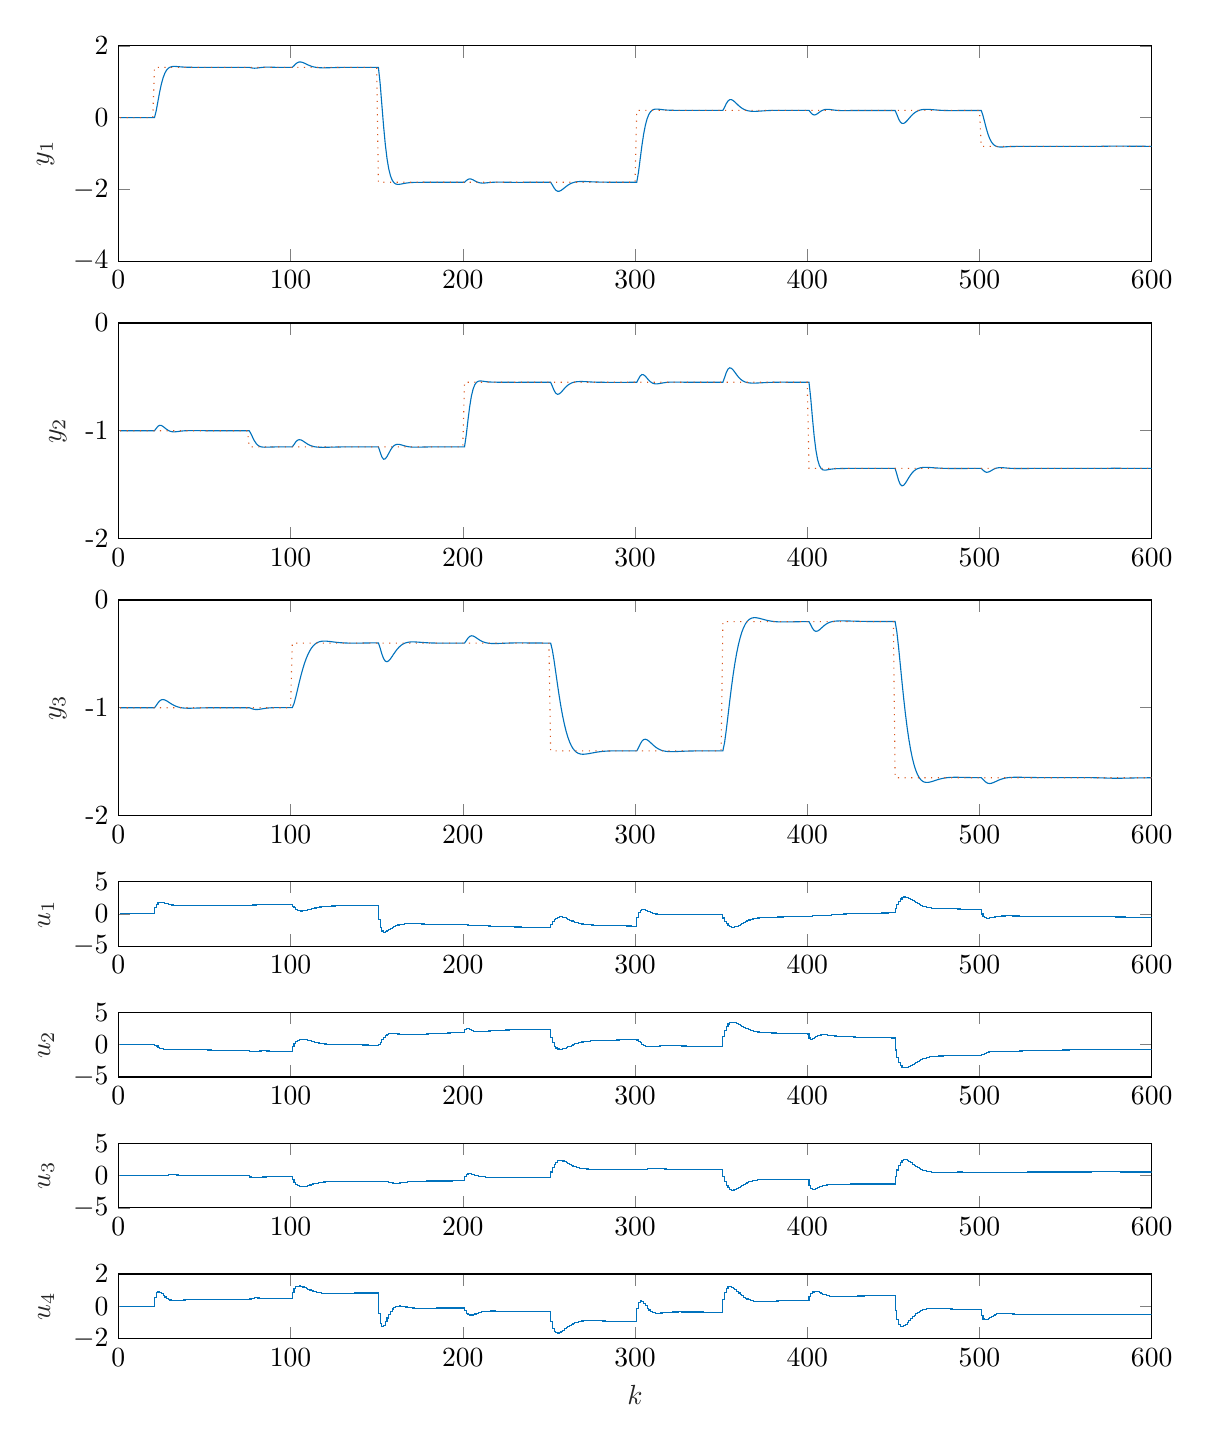
\begin{tikzpicture}

\begin{axis}[%
width=5.167in,
height=0.323in,
at={(0.646in,0.385in)},
scale only axis,
xmin=0,
xmax=600,
xtick={0,100,200,300,400,500,600},
xlabel style={font=\color{white!15!black}},
xlabel={$k$},
ymin=-2,
ymax=2,
ytick={-2,0,2},
ylabel style={font=\color{white!15!black}},
ylabel={$u_4$},
axis background/.style={fill=white}
]
\addplot[const plot, color=mycolor1, forget plot] table[row sep=crcr] {%
1	0\\
2	0\\
3	0\\
4	0\\
5	0\\
6	0\\
7	0\\
8	0\\
9	0\\
10	0\\
11	0\\
12	0\\
13	0\\
14	0\\
15	0\\
16	0\\
17	0\\
18	0\\
19	0\\
20	0\\
21	0.564241952521633\\
22	0.832875647322924\\
23	0.908851870706038\\
24	0.873203605382437\\
25	0.783843953598432\\
26	0.678516161188831\\
27	0.579274920574161\\
28	0.497013453907535\\
29	0.435329073172773\\
30	0.39349715212501\\
31	0.368580909289105\\
32	0.356818554400015\\
33	0.35445992831557\\
34	0.358212893856828\\
35	0.365430785537126\\
36	0.374140127913277\\
37	0.382979117885129\\
38	0.391094295011778\\
39	0.39802548836083\\
40	0.403596719408792\\
41	0.407822218389736\\
42	0.410831108153546\\
43	0.412810828728308\\
44	0.413967398787921\\
45	0.41449966845276\\
46	0.414584459942943\\
47	0.414369657486357\\
48	0.413972704904048\\
49	0.413482463763783\\
50	0.412962886946764\\
51	0.412457417160247\\
52	0.411993399308367\\
53	0.411586090771031\\
54	0.411242068146643\\
55	0.410961973692088\\
56	0.410742633480577\\
57	0.410578626451372\\
58	0.410463401890252\\
59	0.410390043021151\\
60	0.410351764347223\\
61	0.410342215820063\\
62	0.410355651502461\\
63	0.410387006233015\\
64	0.410431911898883\\
65	0.410486675544928\\
66	0.410548234533923\\
67	0.410614098953461\\
68	0.410682288005736\\
69	0.410751264802112\\
70	0.410819872465906\\
71	0.410887273453243\\
72	0.41095289333871\\
73	0.41101636984968\\
74	0.411077507590015\\
75	0.411136238624746\\
76	0.456273683382766\\
77	0.489645788622967\\
78	0.510282405561576\\
79	0.519331634956374\\
80	0.519325099406898\\
81	0.513293004327998\\
82	0.504073411231929\\
83	0.493916343624794\\
84	0.484351461768366\\
85	0.476236536183596\\
86	0.469900418843379\\
87	0.465313233073406\\
88	0.462241500241482\\
89	0.460367999590104\\
90	0.459371877233898\\
91	0.45897368713685\\
92	0.458954000910027\\
93	0.459154725861146\\
94	0.459470903264587\\
95	0.459838683643993\\
96	0.460223113629816\\
97	0.460607680219404\\
98	0.460986356076262\\
99	0.461358143111139\\
100	0.461723724772362\\
101	0.846888806047633\\
102	1.07844833688211\\
103	1.20208475705427\\
104	1.25354758988035\\
105	1.25894198658648\\
106	1.23640960693238\\
107	1.19812084058784\\
108	1.15204912667625\\
109	1.10334207180219\\
110	1.05528818910312\\
111	1.00995613922923\\
112	0.968600397218064\\
113	0.931915182340691\\
114	0.900196836752421\\
115	0.873453829600255\\
116	0.851487290058291\\
117	0.833954096713631\\
118	0.82041816584442\\
119	0.810392334127163\\
120	0.803371884620803\\
121	0.79886040362432\\
122	0.796388701061554\\
123	0.795527664859642\\
124	0.795896013671443\\
125	0.797163926223969\\
126	0.799053470527993\\
127	0.801336658005884\\
128	0.803831831027582\\
129	0.806398975189975\\
130	0.808934440214127\\
131	0.811365459709252\\
132	0.813644779761229\\
133	0.815745635069372\\
134	0.817657241378253\\
135	0.819380893108157\\
136	0.820926652055299\\
137	0.822310474663547\\
138	0.823551447840579\\
139	0.824668603383301\\
140	0.825676613990961\\
141	0.826579654695196\\
142	0.827177709164472\\
143	0.827469549067503\\
144	0.827537501467341\\
145	0.827479801619257\\
146	0.827378517288998\\
147	0.827289694606373\\
148	0.827244986662664\\
149	0.827257651547823\\
150	0.827328988672417\\
151	-0.46224237012219\\
152	-1.07609321787481\\
153	-1.24954940732998\\
154	-1.1678388338216\\
155	-0.963343225426684\\
156	-0.722340759520957\\
157	-0.495248897827846\\
158	-0.306971940600791\\
159	-0.165736581834184\\
160	-0.0698895978115637\\
161	-0.0127202946131315\\
162	0.0143687424666814\\
163	0.0199491684042211\\
164	0.0115463785751727\\
165	-0.00478912773041511\\
166	-0.0245452720767099\\
167	-0.044607932051168\\
168	-0.06302487861818\\
169	-0.0787428870993118\\
170	-0.0913584328882612\\
171	-0.100902906067623\\
172	-0.107670472764444\\
173	-0.112088755343925\\
174	-0.114627984659313\\
175	-0.115742124552856\\
176	-0.115834878729292\\
177	-0.115243866410971\\
178	-0.114237160163091\\
179	-0.113017509151261\\
180	-0.111730718258524\\
181	-0.110475692780302\\
182	-0.109314525678873\\
183	-0.10828167908624\\
184	-0.10739180198091\\
185	-0.106646056180631\\
186	-0.10603702450967\\
187	-0.105552380352457\\
188	-0.10517753559006\\
189	-0.104897477629854\\
190	-0.104697973620789\\
191	-0.104566273548089\\
192	-0.104491392342819\\
193	-0.104464000823506\\
194	-0.104475912402617\\
195	-0.104519125223814\\
196	-0.104584380080268\\
197	-0.104641149705485\\
198	-0.104688507933751\\
199	-0.104735000810808\\
200	-0.104788035380521\\
201	-0.285174434598504\\
202	-0.418515138573533\\
203	-0.500923258180071\\
204	-0.536983407783372\\
205	-0.536814300949423\\
206	-0.512529879422566\\
207	-0.47547675353154\\
208	-0.434650618767251\\
209	-0.396166783485338\\
210	-0.363453880708167\\
211	-0.337825665374512\\
212	-0.319161842532714\\
213	-0.306528823640248\\
214	-0.298659589056963\\
215	-0.294274678934241\\
216	-0.292262956773586\\
217	-0.291756542654025\\
218	-0.292136236861154\\
219	-0.292998176422922\\
220	-0.294104050241639\\
221	-0.295328861040897\\
222	-0.296682083456332\\
223	-0.298146951151435\\
224	-0.299697905617244\\
225	-0.301308492345597\\
226	-0.302953546222521\\
227	-0.304608996419862\\
228	-0.306251362207261\\
229	-0.307857828362414\\
230	-0.30940699392472\\
231	-0.310880000599452\\
232	-0.312261660221517\\
233	-0.313541282335543\\
234	-0.314713045577421\\
235	-0.315775892033089\\
236	-0.316733019939639\\
237	-0.317591100112809\\
238	-0.318359352574739\\
239	-0.319048604679228\\
240	-0.319670423211843\\
241	-0.320236380385856\\
242	-0.320757483804714\\
243	-0.321243776639904\\
244	-0.321704097482036\\
245	-0.322145979102381\\
246	-0.322575660501898\\
247	-0.322998185667227\\
248	-0.323417563996971\\
249	-0.323836970212796\\
250	-0.324258964793253\\
251	-0.966027563744964\\
252	-1.35180333059728\\
253	-1.55772742448724\\
254	-1.64338733555147\\
255	-1.65229731890586\\
256	-1.61469936580034\\
257	-1.55088314301198\\
258	-1.47414285290313\\
259	-1.39306217157265\\
260	-1.31312528655281\\
261	-1.23778216562811\\
262	-1.16912461643277\\
263	-1.10830951099744\\
264	-1.05582972079165\\
265	-1.01169795198429\\
266	-0.975581478255575\\
267	-0.94690744486346\\
268	-0.924947450572461\\
269	-0.90888429553681\\
270	-0.897861185299539\\
271	-0.891013048607031\\
272	-0.887056837711945\\
273	-0.885234931081863\\
274	-0.885065075727379\\
275	-0.886191877029816\\
276	-0.888314026000127\\
277	-0.891158219498568\\
278	-0.894476484107293\\
279	-0.898051684355688\\
280	-0.901703066048009\\
281	-0.905288621092035\\
282	-0.908703903893815\\
283	-0.911878204069827\\
284	-0.91476928467338\\
285	-0.917357716160703\\
286	-0.919641496604933\\
287	-0.921631323836289\\
288	-0.923346646194788\\
289	-0.924812474717109\\
290	-0.926056871573347\\
291	-0.927109010612598\\
292	-0.927997712461309\\
293	-0.928750372426266\\
294	-0.929392215303495\\
295	-0.929945823286873\\
296	-0.930430891005675\\
297	-0.930864166360709\\
298	-0.931259538730715\\
299	-0.931628238502109\\
300	-0.931979114476796\\
301	-0.126259026629355\\
302	0.257169500746816\\
303	0.365375306452265\\
304	0.314117128688466\\
305	0.186126070997917\\
306	0.0353196947827832\\
307	-0.106796280187324\\
308	-0.224660797069481\\
309	-0.313135228633529\\
310	-0.373254747285683\\
311	-0.409214155879797\\
312	-0.426385970960919\\
313	-0.430124884674496\\
314	-0.425129718795993\\
315	-0.41517537921722\\
316	-0.403073225994588\\
317	-0.390759359501121\\
318	-0.379443362362888\\
319	-0.369774823435838\\
320	-0.362002767533773\\
321	-0.356115211588719\\
322	-0.352026199870487\\
323	-0.349452478041365\\
324	-0.348050074750824\\
325	-0.34749281797463\\
326	-0.347508156307398\\
327	-0.347886209550691\\
328	-0.348474686258598\\
329	-0.349168139780199\\
330	-0.349896429503035\\
331	-0.35061468470246\\
332	-0.351295497703147\\
333	-0.351923260573998\\
334	-0.352490236055088\\
335	-0.352993899417977\\
336	-0.353435154579269\\
337	-0.353817128692256\\
338	-0.35414434308997\\
339	-0.354422130484045\\
340	-0.354656218184821\\
341	-0.35485242953013\\
342	-0.355016476107471\\
343	-0.355153836240107\\
344	-0.355269670400815\\
345	-0.355368764111349\\
346	-0.355455497934285\\
347	-0.355533846420629\\
348	-0.355607406640512\\
349	-0.355679454587736\\
350	-0.355753025594463\\
351	0.413779200505231\\
352	0.876104640099562\\
353	1.12258731572017\\
354	1.22472643608275\\
355	1.23473268517654\\
356	1.18888925443873\\
357	1.11153576442683\\
358	1.0186166466008\\
359	0.920423395310466\\
360	0.82352832328118\\
361	0.73206356441947\\
362	0.648533153555039\\
363	0.574321835987221\\
364	0.510020943227741\\
365	0.455649619151141\\
366	0.410817071460097\\
367	0.374849670498257\\
368	0.346893804003415\\
369	0.325998720511755\\
370	0.31118070538949\\
371	0.301469061719111\\
372	0.296048817366629\\
373	0.294071508636415\\
374	0.29473605446002\\
375	0.297331430493846\\
376	0.301252924901473\\
377	0.306002629999691\\
378	0.311181911774339\\
379	0.316480644276599\\
380	0.321665733539224\\
381	0.326570021827887\\
382	0.331081909809613\\
383	0.335135731184463\\
384	0.338702853510846\\
385	0.341783513625656\\
386	0.344399442061786\\
387	0.346587351969151\\
388	0.348393357704873\\
389	0.349868354455175\\
390	0.35106434536892\\
391	0.352031658116074\\
392	0.352816957035262\\
393	0.353461795011693\\
394	0.354002029423598\\
395	0.354467759730724\\
396	0.354883578471235\\
397	0.355269014155849\\
398	0.355639092369154\\
399	0.356004964555075\\
400	0.356374564672783\\
401	0.597185763974688\\
402	0.775273205804487\\
403	0.885464069007938\\
404	0.933881820972178\\
405	0.934028138599776\\
406	0.902063586721954\\
407	0.853123979601908\\
408	0.799209071907247\\
409	0.748476850806356\\
410	0.705502009711796\\
411	0.672038364629067\\
412	0.647926437558204\\
413	0.631920756502752\\
414	0.622329165111334\\
415	0.617440236538323\\
416	0.615763691759562\\
417	0.616129663184542\\
418	0.617695109294551\\
419	0.619898134363878\\
420	0.622389678416957\\
421	0.624961025883134\\
422	0.627212285463564\\
423	0.629086220586764\\
424	0.630674804047257\\
425	0.632104773762336\\
426	0.633482274333941\\
427	0.634874811897411\\
428	0.636312931414953\\
429	0.637799788455383\\
430	0.639321892559141\\
431	0.640857957436023\\
432	0.642385007377784\\
433	0.64388199435819\\
434	0.645331573000805\\
435	0.646720691236626\\
436	0.648040508624497\\
437	0.649285981092435\\
438	0.650455308995011\\
439	0.651549350625827\\
440	0.652571050032632\\
441	0.653524903244385\\
442	0.654416478081264\\
443	0.655252036087078\\
444	0.656038141715175\\
445	0.656781332334898\\
446	0.657487878937096\\
447	0.658163640841396\\
448	0.658814004699556\\
449	0.659443893502061\\
450	0.660057830839999\\
451	-0.269285628471088\\
452	-0.82743733525571\\
453	-1.12479498573733\\
454	-1.24775305604736\\
455	-1.25939913134647\\
456	-1.20357513143413\\
457	-1.10969119501716\\
458	-0.997013288474306\\
459	-0.877976743732192\\
460	-0.760522865682769\\
461	-0.649644382684351\\
462	-0.548366700394514\\
463	-0.458362705493464\\
464	-0.380346525182597\\
465	-0.314340835669429\\
466	-0.259872910575186\\
467	-0.216128195597063\\
468	-0.182074593325309\\
469	-0.156562577047073\\
470	-0.138402763546226\\
471	-0.126421522889589\\
472	-0.119632542960206\\
473	-0.117009983792727\\
474	-0.117585654681377\\
475	-0.120500281880188\\
476	-0.125023020775337\\
477	-0.130552011735634\\
478	-0.136605282338832\\
479	-0.142807750706131\\
480	-0.148877367937674\\
481	-0.154611715288778\\
482	-0.159875466214759\\
483	-0.164588758255798\\
484	-0.168716445365936\\
485	-0.172258241641702\\
486	-0.175239821640409\\
487	-0.177704967226981\\
488	-0.179708838431828\\
489	-0.181312405793616\\
490	-0.18257802882016\\
491	-0.183566112635604\\
492	-0.184332731560232\\
493	-0.184928061768699\\
494	-0.185395537906506\\
495	-0.185771587954112\\
496	-0.186085798162251\\
497	-0.186361373308938\\
498	-0.186615779104403\\
499	-0.18686147741355\\
500	-0.187106687541591\\
501	-0.590386092627286\\
502	-0.782522874662869\\
503	-0.837053020081327\\
504	-0.811855294490579\\
505	-0.748293092127527\\
506	-0.673322012567101\\
507	-0.602691166459226\\
508	-0.544177161534828\\
509	-0.500345576077874\\
510	-0.470675609999885\\
511	-0.453067500437389\\
512	-0.444833813424425\\
513	-0.443297541184614\\
514	-0.446111417862741\\
515	-0.451392135673338\\
516	-0.457740145045619\\
517	-0.464195123955291\\
518	-0.470160625526178\\
519	-0.475318946133244\\
520	-0.479548361002476\\
521	-0.482848875706077\\
522	-0.485182461456996\\
523	-0.486704805980413\\
524	-0.487630485720898\\
525	-0.488158908560379\\
526	-0.488444226498567\\
527	-0.488591483085962\\
528	-0.48866517024464\\
529	-0.488701335361685\\
530	-0.488718588415104\\
531	-0.488726243328316\\
532	-0.48872947043339\\
533	-0.488732069029861\\
534	-0.488737645253767\\
535	-0.488749880513447\\
536	-0.488772381509821\\
537	-0.488808412412637\\
538	-0.488860663155634\\
539	-0.488931111603147\\
540	-0.489020982790653\\
541	-0.489130782782982\\
542	-0.489260376901388\\
543	-0.489408996995837\\
544	-0.489575437303903\\
545	-0.489758288094517\\
546	-0.489956140945492\\
547	-0.490167750118018\\
548	-0.490392157889039\\
549	-0.490628798081367\\
550	-0.490877589981852\\
551	-0.491139029860155\\
552	-0.491414282092577\\
553	-0.491705267259636\\
554	-0.492014740336711\\
555	-0.492346347720676\\
556	-0.492704646883664\\
557	-0.493095066726014\\
558	-0.493523780371499\\
559	-0.493997455795216\\
560	-0.494522844455917\\
561	-0.495106166004073\\
562	-0.495752251361456\\
563	-0.496463421966036\\
564	-0.497238116995014\\
565	-0.498069342636589\\
566	-0.498943120069161\\
567	-0.499837263783897\\
568	-0.500721036660194\\
569	-0.501556496369011\\
570	-0.502302633980189\\
571	-0.50292362428037\\
572	-0.503236688698695\\
573	-0.503223651177892\\
574	-0.502936079492999\\
575	-0.502443888332475\\
576	-0.501813016546647\\
577	-0.501099139542915\\
578	-0.500348256460421\\
579	-0.499598924691515\\
580	-0.498883863769427\\
581	-0.498230432400919\\
582	-0.497660314469888\\
583	-0.497188965208309\\
584	-0.496825266492653\\
585	-0.496571630618185\\
586	-0.496424594609261\\
587	-0.496375812577706\\
588	-0.496413289115669\\
589	-0.496522688183086\\
590	-0.496688578907312\\
591	-0.496895523279426\\
592	-0.49712895688021\\
593	-0.497375874321944\\
594	-0.497625255937792\\
595	-0.497868261954913\\
596	-0.498098243012668\\
597	-0.498310620367388\\
598	-0.49850268345219\\
599	-0.498673342796303\\
600	-0.498822866348315\\
};
\end{axis}

\begin{axis}[%
width=5.167in,
height=0.323in,
at={(0.646in,1.039in)},
scale only axis,
xmin=0,
xmax=600,
xtick={0,100,200,300,400,500,600},
ymin=-5,
ymax=5,
ytick={-5,0,5},
ylabel style={font=\color{white!15!black}},
ylabel={$u_3$},
axis background/.style={fill=white}
]
\addplot[const plot, color=mycolor1, forget plot] table[row sep=crcr] {%
1	0\\
2	0\\
3	0\\
4	0\\
5	0\\
6	0\\
7	0\\
8	0\\
9	0\\
10	0\\
11	0\\
12	0\\
13	0\\
14	0\\
15	0\\
16	0\\
17	0\\
18	0\\
19	0\\
20	0\\
21	0.0146357184272746\\
22	-0.00156394241370302\\
23	-0.0189475819732245\\
24	-0.0229359849042252\\
25	-0.0107898511545217\\
26	0.013267808296143\\
27	0.0423868051050337\\
28	0.0700398029255049\\
29	0.0915431157551111\\
30	0.104475618562225\\
31	0.108417381308339\\
32	0.10437626368621\\
33	0.0941612966318092\\
34	0.0798504720386962\\
35	0.0634129611842653\\
36	0.0464884820405927\\
37	0.0302961872677999\\
38	0.0156347587596408\\
39	0.00293677852958387\\
40	-0.00765225514609172\\
41	-0.0161908924755449\\
42	-0.0228670219275337\\
43	-0.0279373579322104\\
44	-0.031682562648218\\
45	-0.034376792513697\\
46	-0.0362691766908942\\
47	-0.037574367248098\\
48	-0.0384694739579345\\
49	-0.0390951321988837\\
50	-0.0395589678551025\\
51	-0.0399402124332788\\
52	-0.040294634037527\\
53	-0.0406592698686004\\
54	-0.0410566780311398\\
55	-0.0414985844861951\\
56	-0.0419889015530535\\
57	-0.0425261531177058\\
58	-0.0431053717741844\\
59	-0.0437195446574255\\
60	-0.044360685089633\\
61	-0.045020601416972\\
62	-0.0456914258494598\\
63	-0.0463659567432343\\
64	-0.0470378587117447\\
65	-0.0477017567799365\\
66	-0.0483532537117469\\
67	-0.0489888936556965\\
68	-0.0496060902753941\\
69	-0.0502030334311353\\
70	-0.0507785851201989\\
71	-0.0513321726437701\\
72	-0.0518636847431607\\
73	-0.0523733746518434\\
74	-0.052861772574103\\
75	-0.053329608970301\\
76	-0.233415377184642\\
77	-0.316014625677202\\
78	-0.339298508849092\\
79	-0.331199981037117\\
80	-0.309823266322483\\
81	-0.285539713006325\\
82	-0.26340887085228\\
83	-0.245260029363748\\
84	-0.231212327656009\\
85	-0.220650825548076\\
86	-0.21277639507112\\
87	-0.206866448105446\\
88	-0.20236347848477\\
89	-0.198875666798658\\
90	-0.196142482356634\\
91	-0.193994078384203\\
92	-0.192317253352773\\
93	-0.191031517175723\\
94	-0.190074346555927\\
95	-0.189393171510601\\
96	-0.188941600514718\\
97	-0.188677959468922\\
98	-0.188564890270538\\
99	-0.18856930622509\\
100	-0.188662374757947\\
101	-0.6826330642627\\
102	-1.08639724074558\\
103	-1.39052390829323\\
104	-1.5966651753244\\
105	-1.71526207137886\\
106	-1.76188000907327\\
107	-1.75379361192778\\
108	-1.70749624557555\\
109	-1.637238486659\\
110	-1.55441933465857\\
111	-1.46756425447059\\
112	-1.38263938523778\\
113	-1.30351063869961\\
114	-1.23242330457951\\
115	-1.17043416811986\\
116	-1.11776815039702\\
117	-1.07409588876868\\
118	-1.03874107059401\\
119	-1.01083080268783\\
120	-0.989402292722367\\
121	-0.973477086498013\\
122	-0.962111542659262\\
123	-0.954429898122239\\
124	-0.949644466973005\\
125	-0.9470662379679\\
126	-0.946108286741726\\
127	-0.946283865176618\\
128	-0.947200655415365\\
129	-0.948552395933019\\
130	-0.950108851498639\\
131	-0.951704884626259\\
132	-0.953229190272178\\
133	-0.95461308981706\\
134	-0.955819667713449\\
135	-0.956833506034544\\
136	-0.957651364123469\\
137	-0.958274392786962\\
138	-0.958702870849918\\
139	-0.958934955815265\\
140	-0.958971395965334\\
141	-0.958828243555714\\
142	-0.958456092920336\\
143	-0.957821338582337\\
144	-0.956932075058401\\
145	-0.955838858382766\\
146	-0.954620441937942\\
147	-0.953364827543463\\
148	-0.952152720292656\\
149	-0.951046729689925\\
150	-0.950086787737603\\
151	-0.982743669358246\\
152	-0.945082591092076\\
153	-0.90486395247884\\
154	-0.89538937750179\\
155	-0.922894389294469\\
156	-0.977700759521508\\
157	-1.04412775779077\\
158	-1.10723640264024\\
159	-1.15630607033155\\
160	-1.18579191495489\\
161	-1.1947270020189\\
162	-1.18541101894747\\
163	-1.16197729607671\\
164	-1.12917564629481\\
165	-1.09150826503313\\
166	-1.0527249331341\\
167	-1.0156143785866\\
168	-0.982004216102305\\
169	-0.952885039920002\\
170	-0.928590925871697\\
171	-0.908989180914223\\
172	-0.893651109677765\\
173	-0.881990360907242\\
174	-0.873365560095931\\
175	-0.867149983568657\\
176	-0.862773965273177\\
177	-0.859746568662321\\
178	-0.857662661739646\\
179	-0.856200538385926\\
180	-0.855114051280801\\
181	-0.854222103195312\\
182	-0.853397400460731\\
183	-0.852555640653933\\
184	-0.851645776000125\\
185	-0.850641633357938\\
186	-0.849534943334568\\
187	-0.848329699446494\\
188	-0.847037703218149\\
189	-0.845675129001846\\
190	-0.844259945180308\\
191	-0.842810042995929\\
192	-0.841341940908698\\
193	-0.839869944733916\\
194	-0.838405649217753\\
195	-0.836957667863973\\
196	-0.835531485250014\\
197	-0.834103067781558\\
198	-0.832665620125913\\
199	-0.831221784158971\\
200	-0.829779165914047\\
201	-0.109797357617998\\
202	0.220290901770028\\
203	0.313155081316657\\
204	0.280512461213923\\
205	0.194766537535661\\
206	0.0973906490662662\\
207	0.00861219761609777\\
208	-0.0642615133408168\\
209	-0.120763268048281\\
210	-0.163362071694751\\
211	-0.195263875595064\\
212	-0.219368745075452\\
213	-0.237916508783419\\
214	-0.252483888617141\\
215	-0.264121397680064\\
216	-0.273514863352472\\
217	-0.28112051143275\\
218	-0.287259425434938\\
219	-0.292174897639547\\
220	-0.296062186892604\\
221	-0.29908014313477\\
222	-0.301096312388703\\
223	-0.302118272174928\\
224	-0.302248717811742\\
225	-0.301644910134317\\
226	-0.300485957437645\\
227	-0.298949128955179\\
228	-0.29719467008237\\
229	-0.295357616990564\\
230	-0.293544786065477\\
231	-0.29183522192251\\
232	-0.29028271011629\\
233	-0.288919337395088\\
234	-0.287759420557811\\
235	-0.286803386254694\\
236	-0.286041365230195\\
237	-0.285456379880612\\
238	-0.28502707298349\\
239	-0.284729965465759\\
240	-0.284541254760472\\
241	-0.284438180392051\\
242	-0.284399993854813\\
243	-0.284408577148059\\
244	-0.28444875886804\\
245	-0.284508378546131\\
246	-0.284578149063767\\
247	-0.284651363803813\\
248	-0.284723490263392\\
249	-0.284791685819081\\
250	-0.28485426488364\\
251	0.538112612206397\\
252	1.21067100709525\\
253	1.71713263052226\\
254	2.06027653908197\\
255	2.25752659365322\\
256	2.33484496139762\\
257	2.32104114847757\\
258	2.24362205982242\\
259	2.1263567112742\\
260	1.98826179465019\\
261	1.84356472028331\\
262	1.70222613812799\\
263	1.57070279422533\\
264	1.45274357392822\\
265	1.35010541781345\\
266	1.26314295701328\\
267	1.19126716637359\\
268	1.13329006841147\\
269	1.08768123427736\\
270	1.05276292697361\\
271	1.02686758864069\\
272	1.00824050197921\\
273	0.995282498221988\\
274	0.986643690758538\\
275	0.981242995996468\\
276	0.978240800971563\\
277	0.976991713470241\\
278	0.97699625596708\\
279	0.97786133046341\\
280	0.979272329346183\\
281	0.980975636995137\\
282	0.982768535082449\\
283	0.984493378359726\\
284	0.986033570785751\\
285	0.987309778972848\\
286	0.988275641347837\\
287	0.988912825862131\\
288	0.989225637298562\\
289	0.989235520812784\\
290	0.988975815848549\\
291	0.98848704507009\\
292	0.987812923298102\\
293	0.986997172042345\\
294	0.986081142426925\\
295	0.985102189263492\\
296	0.984092701581657\\
297	0.983079676639099\\
298	0.98208472066927\\
299	0.981124365767897\\
300	0.980210604382524\\
301	1.00025972688125\\
302	0.976318006049521\\
303	0.950747176926498\\
304	0.944375602947365\\
305	0.961116454414677\\
306	0.994936274883151\\
307	1.03604847884276\\
308	1.07512800090744\\
309	1.10548404459704\\
310	1.12365855512177\\
311	1.12905271649727\\
312	1.12310753622003\\
313	1.10840829356763\\
314	1.08792378004702\\
315	1.06446612990694\\
316	1.04037518519128\\
317	1.01738797153069\\
318	0.996638551492016\\
319	0.978735459563376\\
320	0.963874255676844\\
321	0.951955564822575\\
322	0.942585714172134\\
323	0.935349283248574\\
324	0.929840822001464\\
325	0.925689096066367\\
326	0.922572205094479\\
327	0.920223733167787\\
328	0.918431673285152\\
329	0.917032621605315\\
330	0.91590369677418\\
331	0.914954103538117\\
332	0.914117549547951\\
333	0.913346071621543\\
334	0.912605349975757\\
335	0.911871310348422\\
336	0.911127702675269\\
337	0.910364346791263\\
338	0.909575796835565\\
339	0.908760255432976\\
340	0.907918640746541\\
341	0.907053762402144\\
342	0.906169594194705\\
343	0.905270552911569\\
344	0.904361017613922\\
345	0.903445028210952\\
346	0.902526121601486\\
347	0.901607278237107\\
348	0.900690961541906\\
349	0.899779238108862\\
350	0.898873969148877\\
351	-0.0896502389441057\\
352	-0.89766432999633\\
353	-1.50633749043998\\
354	-1.91899736050847\\
355	-2.15654199051686\\
356	-2.25011113004926\\
357	-2.23425630701085\\
358	-2.1419603981982\\
359	-2.00171519274488\\
360	-1.83630459336555\\
361	-1.66276166201333\\
362	-1.49299820194308\\
363	-1.3347243264329\\
364	-1.19240923042847\\
365	-1.06814713606872\\
366	-0.96237239004001\\
367	-0.874416538765213\\
368	-0.802925099443587\\
369	-0.746160872832171\\
370	-0.702220909664575\\
371	-0.669190493515605\\
372	-0.645678330772683\\
373	-0.630166113071782\\
374	-0.621123700646679\\
375	-0.6170976494339\\
376	-0.61677291015645\\
377	-0.619009539509768\\
378	-0.622858168901739\\
379	-0.627559037745306\\
380	-0.632529548433087\\
381	-0.637344784223614\\
382	-0.641714567247921\\
383	-0.64545968644012\\
384	-0.64848906369879\\
385	-0.650778930831678\\
386	-0.652354575027898\\
387	-0.653274856016338\\
388	-0.653619468742757\\
389	-0.653478785916596\\
390	-0.652946035892825\\
391	-0.65211153166406\\
392	-0.651058651693727\\
393	-0.649860986638462\\
394	-0.648581035631781\\
395	-0.647269993693189\\
396	-0.645968264187151\\
397	-0.644706420809769\\
398	-0.643506422019253\\
399	-0.642382942516323\\
400	-0.641344731374686\\
401	-1.59846328696718\\
402	-2.03584395894148\\
403	-2.15705961020247\\
404	-2.11107821207184\\
405	-1.99444774126658\\
406	-1.86247495491776\\
407	-1.74213850483943\\
408	-1.64319097546252\\
409	-1.56626639675114\\
410	-1.50808591257484\\
411	-1.46439009321299\\
412	-1.43132852462843\\
413	-1.40593043990832\\
414	-1.38610564784786\\
415	-1.37045814874629\\
416	-1.35806637094793\\
417	-1.34829896870412\\
418	-1.34068652943895\\
419	-1.33484656137871\\
420	-1.33045159488628\\
421	-1.32723019653591\\
422	-1.32484584722227\\
423	-1.32301216447636\\
424	-1.32153034330914\\
425	-1.3202903745128\\
426	-1.31924999995882\\
427	-1.3184062182528\\
428	-1.31776968221742\\
429	-1.31734698241853\\
430	-1.31713165431925\\
431	-1.31710232527706\\
432	-1.31722549634103\\
433	-1.31746052547267\\
434	-1.31776494824957\\
435	-1.31809897546772\\
436	-1.3184286312849\\
437	-1.31872745002404\\
438	-1.31897692390725\\
439	-1.31916601888376\\
440	-1.31929009651577\\
441	-1.31934953975751\\
442	-1.31934831325052\\
443	-1.31929259450651\\
444	-1.31918964141997\\
445	-1.31904692068668\\
446	-1.31887149820256\\
447	-1.31866967560329\\
448	-1.31844684627138\\
449	-1.31820753872827\\
450	-1.31795561412377\\
451	-0.124311594543726\\
452	0.851234401882558\\
453	1.58592794032603\\
454	2.0837896284399\\
455	2.37007116869518\\
456	2.48239977653208\\
457	2.462525310354\\
458	2.35030221208627\\
459	2.18015819740795\\
460	1.97962393260612\\
461	1.76928111330961\\
462	1.5635231966546\\
463	1.37166653797773\\
464	1.19911131720173\\
465	1.04838788547946\\
466	0.920020837880563\\
467	0.813202142484483\\
468	0.726294733408961\\
469	0.657199003409041\\
470	0.603614950950532\\
471	0.563228204049104\\
472	0.53435309404406\\
473	0.515152683468507\\
474	0.503777321881692\\
475	0.498471051695733\\
476	0.497645698554035\\
477	0.499924886135401\\
478	0.504162495724981\\
479	0.509441360469336\\
480	0.515058160904841\\
481	0.520499866143828\\
482	0.525416025349767\\
483	0.529590074499989\\
484	0.532911787177645\\
485	0.535352160852806\\
486	0.536941410384601\\
487	0.537750313409252\\
488	0.537874875924549\\
489	0.537424118317598\\
490	0.536510687391248\\
491	0.535243953247535\\
492	0.533725234083479\\
493	0.53204495134108\\
494	0.530280998107513\\
495	0.528498116752076\\
496	0.526748072315399\\
497	0.525070411076691\\
498	0.523493609234074\\
499	0.52203644184113\\
500	0.520709433000281\\
501	0.509062196390301\\
502	0.519572285212963\\
503	0.531054004058258\\
504	0.533084194764753\\
505	0.523694316399385\\
506	0.505887135078107\\
507	0.484540770889595\\
508	0.464302021472975\\
509	0.44850052381462\\
510	0.438849978666574\\
511	0.435635319803722\\
512	0.438122819425976\\
513	0.445008250637518\\
514	0.454797635211912\\
515	0.466077655560872\\
516	0.477673729267355\\
517	0.488715436084114\\
518	0.498636667424056\\
519	0.507136960669228\\
520	0.514125360059193\\
521	0.519661760416457\\
522	0.52404489124454\\
523	0.527520863033918\\
524	0.530294226023895\\
525	0.532531834223106\\
526	0.534364686217023\\
527	0.535890933708593\\
528	0.537180932005399\\
529	0.538283683141231\\
530	0.539233462588406\\
531	0.540055552894344\\
532	0.54077046377515\\
533	0.541396507582653\\
534	0.541950960018575\\
535	0.542450219653328\\
536	0.542909408926144\\
537	0.543341787539245\\
538	0.543758232358849\\
539	0.544166918870577\\
540	0.544573243049458\\
541	0.544979958642637\\
542	0.54538747179426\\
543	0.545794046024445\\
544	0.546196275467682\\
545	0.546589659753716\\
546	0.546969172026564\\
547	0.547329764759528\\
548	0.547666799079424\\
549	0.547976409812551\\
550	0.548255831466992\\
551	0.548503712743328\\
552	0.548720442163401\\
553	0.548908497754934\\
554	0.54907282131516\\
555	0.549221203734065\\
556	0.549364652913657\\
557	0.549517700737893\\
558	0.549698591560116\\
559	0.549929283785554\\
560	0.550235191171691\\
561	0.550644594771973\\
562	0.551187672886097\\
563	0.551895125699143\\
564	0.552796409639763\\
565	0.5539176323064\\
566	0.555279170377253\\
567	0.556893027407245\\
568	0.558759806210346\\
569	0.560864898305247\\
570	0.563173090199505\\
571	0.565620329242825\\
572	0.567483760800603\\
573	0.568420383752536\\
574	0.568358202458986\\
575	0.56739816531948\\
576	0.56573417499836\\
577	0.563593950116011\\
578	0.561199696244629\\
579	0.558745233597322\\
580	0.556385381159725\\
581	0.554233582488566\\
582	0.552364489533834\\
583	0.55081911280388\\
584	0.5496109625046\\
585	0.548732240291597\\
586	0.548159578646658\\
587	0.547859095800248\\
588	0.547790685836841\\
589	0.547911540734911\\
590	0.548178937293226\\
591	0.548552338700486\\
592	0.548994869686192\\
593	0.549474044615043\\
594	0.549962277620839\\
595	0.550437123376639\\
596	0.550881248153016\\
597	0.551282168160192\\
598	0.55163181318712\\
599	0.551925980194457\\
600	0.552163737790339\\
};
\end{axis}

\begin{axis}[%
width=5.167in,
height=0.323in,
at={(0.646in,1.693in)},
scale only axis,
xmin=0,
xmax=600,
xtick={0,100,200,300,400,500,600},
ymin=-5,
ymax=5,
ytick={-5,0,5},
ylabel style={font=\color{white!15!black}},
ylabel={$u_2$},
axis background/.style={fill=white}
]
\addplot[const plot, color=mycolor1, forget plot] table[row sep=crcr] {%
1	0\\
2	0\\
3	0\\
4	0\\
5	0\\
6	0\\
7	0\\
8	0\\
9	0\\
10	0\\
11	0\\
12	0\\
13	0\\
14	0\\
15	0\\
16	0\\
17	0\\
18	0\\
19	0\\
20	0\\
21	-0.0567756734872436\\
22	-0.202087707050847\\
23	-0.373211647291838\\
24	-0.529663850119427\\
25	-0.65171703681715\\
26	-0.734719686686972\\
27	-0.782896384625715\\
28	-0.804352784971971\\
29	-0.807771334258393\\
30	-0.800632527157108\\
31	-0.788545813693078\\
32	-0.775255174377081\\
33	-0.762971785814726\\
34	-0.752801718392354\\
35	-0.745139448901411\\
36	-0.739972794803709\\
37	-0.737090923602779\\
38	-0.736210229436337\\
39	-0.73704065117113\\
40	-0.739314112905573\\
41	-0.742792062274137\\
42	-0.747263577483165\\
43	-0.752540753127604\\
44	-0.758454611151876\\
45	-0.76485260629587\\
46	-0.771597639815944\\
47	-0.778568034064481\\
48	-0.785657864623997\\
49	-0.792777182769208\\
50	-0.799851853079795\\
51	-0.806822905578463\\
52	-0.813645428601528\\
53	-0.820287103364446\\
54	-0.82672651232544\\
55	-0.832951353781466\\
56	-0.838956677057432\\
57	-0.844743226061005\\
58	-0.850315950728284\\
59	-0.855682720118033\\
60	-0.86085324967655\\
61	-0.865838239123568\\
62	-0.870648706273857\\
63	-0.875295495235201\\
64	-0.879788933967808\\
65	-0.884138615306585\\
66	-0.8883532764756\\
67	-0.892440754226989\\
68	-0.896407995509836\\
69	-0.900261106636566\\
70	-0.904005426991312\\
71	-0.907645616231116\\
72	-0.91118574655245\\
73	-0.914629393871952\\
74	-0.917979723681232\\
75	-0.9212395688886\\
76	-1.04184790997769\\
77	-1.07716100147143\\
78	-1.06651014047468\\
79	-1.03750956306894\\
80	-1.00669316275685\\
81	-0.982137647484638\\
82	-0.96640493556971\\
83	-0.959004700470555\\
84	-0.958128133235357\\
85	-0.961697646611924\\
86	-0.967896173132216\\
87	-0.97535700121958\\
88	-0.98316436798517\\
89	-0.990769917802341\\
90	-0.997888358136945\\
91	-1.00440418970087\\
92	-1.01030108653942\\
93	-1.01561432958667\\
94	-1.02040182793446\\
95	-1.02472812824512\\
96	-1.02865651085911\\
97	-1.03224559342806\\
98	-1.03554816100628\\
99	-1.03861094687053\\
100	-1.04147475250897\\
101	-0.277080708194094\\
102	0.223128915566238\\
103	0.534520954946309\\
104	0.715626834208581\\
105	0.808358721320422\\
106	0.841293292378347\\
107	0.833555417122436\\
108	0.798124131932158\\
109	0.7441929128656\\
110	0.678642272966416\\
111	0.606850361335052\\
112	0.533087052259466\\
113	0.460689095802785\\
114	0.392147746353667\\
115	0.329181299033343\\
116	0.272822542271279\\
117	0.223525659136859\\
118	0.181284952881826\\
119	0.145754354863878\\
120	0.116358007855007\\
121	0.0923854545959225\\
122	0.0730683803732127\\
123	0.0576386207796928\\
124	0.0453689935383686\\
125	0.0355995096729007\\
126	0.027751864445441\\
127	0.0213350267490222\\
128	0.0159444294101673\\
129	0.0112568527962361\\
130	0.00702267963330013\\
131	0.00305682691277113\\
132	-0.000770654526340407\\
133	-0.00454359140057046\\
134	-0.0083078430788898\\
135	-0.0120784193462231\\
136	-0.0158457565490152\\
137	-0.0195818712606698\\
138	-0.0232478085770392\\
139	-0.0268046283621419\\
140	-0.0302309377093195\\
141	-0.0335502605371768\\
142	-0.0374563782991479\\
143	-0.0420681176228781\\
144	-0.0472247882200842\\
145	-0.0526755369885032\\
146	-0.0581822874364931\\
147	-0.0635634565590487\\
148	-0.0687027611132404\\
149	-0.0735408638544423\\
150	-0.0780609954779627\\
151	0.0474984369376565\\
152	0.375705669195216\\
153	0.76315540870539\\
154	1.11727690025347\\
155	1.39294456394512\\
156	1.57949577903123\\
157	1.68656116583184\\
158	1.73264754334744\\
159	1.73758501601527\\
160	1.71846072038894\\
161	1.68808877811906\\
162	1.65502230235541\\
163	1.62431306120102\\
164	1.59848842323813\\
165	1.57845025796581\\
166	1.5641714754723\\
167	1.55517112827241\\
168	1.55080187865171\\
169	1.55040141769445\\
170	1.55335737772773\\
171	1.55912452399214\\
172	1.56722043063838\\
173	1.57721496590525\\
174	1.58872099650373\\
175	1.60138874741452\\
176	1.61490361412712\\
177	1.62898617196317\\
178	1.64339300084277\\
179	1.65791725598103\\
180	1.6723883546865\\
181	1.68667054871353\\
182	1.7006604413577\\
183	1.71428367861721\\
184	1.72749111349992\\
185	1.74025474111477\\
186	1.75256365793999\\
187	1.76442023452613\\
188	1.77583662334021\\
189	1.78683166345399\\
190	1.79742819840086\\
191	1.80765079742869\\
192	1.81752386656367\\
193	1.8270701553627\\
194	1.83630970510391\\
195	1.84525933422277\\
196	1.85393279447558\\
197	1.86230237730529\\
198	1.87035311639353\\
199	1.87808739331338\\
200	1.88552269772096\\
201	2.36243163313619\\
202	2.49826014568697\\
203	2.4503537369266\\
204	2.32918622220679\\
205	2.20090565536132\\
206	2.09782736249557\\
207	2.03020469435712\\
208	1.99608064167493\\
209	1.98822424651211\\
210	1.99833050482704\\
211	2.01913826709027\\
212	2.04518985972535\\
213	2.0728332573469\\
214	2.09988718315637\\
215	2.1252223890813\\
216	2.14838655928616\\
217	2.1693191394645\\
218	2.18815785699447\\
219	2.20511948256914\\
220	2.2204332259105\\
221	2.23430839501481\\
222	2.24663313755109\\
223	2.25747795555455\\
224	2.26700810731907\\
225	2.27542809503077\\
226	2.2829490849333\\
227	2.28977092480437\\
228	2.29607274035993\\
229	2.30200839142814\\
230	2.30770475971153\\
231	2.31326185504575\\
232	2.31875422438631\\
233	2.32423333247043\\
234	2.3297306228189\\
235	2.33526096827928\\
236	2.3408262325214\\
237	2.34641870151919\\
238	2.35202420141171\\
239	2.35762478404879\\
240	2.36320092272433\\
241	2.36873321078301\\
242	2.37420359193975\\
243	2.37959617354119\\
244	2.38489768482484\\
245	2.3900976444556\\
246	2.39518829817649\\
247	2.40016438079461\\
248	2.40502274885347\\
249	2.40976192260436\\
250	2.41438156923425\\
251	1.14039201179595\\
252	0.306814560361776\\
253	-0.21200334167056\\
254	-0.513648447768271\\
255	-0.668003218361578\\
256	-0.722720012304823\\
257	-0.709695080562945\\
258	-0.650579585192024\\
259	-0.560714311494138\\
260	-0.451584814928379\\
261	-0.332173232880773\\
262	-0.209616070723994\\
263	-0.0894972974337588\\
264	0.0240037453064448\\
265	0.127989235260411\\
266	0.220695366449263\\
267	0.301314648638108\\
268	0.369803893582101\\
269	0.42670125032605\\
270	0.472975114947592\\
271	0.509922961087588\\
272	0.540469213383852\\
273	0.566220038089325\\
274	0.5880692354616\\
275	0.606586777389929\\
276	0.622229905084682\\
277	0.635434064059306\\
278	0.646634935217904\\
279	0.656258553303719\\
280	0.664702130752297\\
281	0.672317098794002\\
282	0.679398664389859\\
283	0.686182214674074\\
284	0.692845164311592\\
285	0.699512407416487\\
286	0.706263729552337\\
287	0.713141942635124\\
288	0.720160913702967\\
289	0.727312984657786\\
290	0.734575511284694\\
291	0.741916402626685\\
292	0.749298639257041\\
293	0.756683810661603\\
294	0.764034750983875\\
295	0.771317376442952\\
296	0.778501840857517\\
297	0.785563130126728\\
298	0.792481213814836\\
299	0.799240863678967\\
300	0.805831236674306\\
301	0.731137200309723\\
302	0.529782478172887\\
303	0.291372037543759\\
304	0.0737400502398845\\
305	-0.0949301241717785\\
306	-0.207991385991865\\
307	-0.271476787757842\\
308	-0.296964234413917\\
309	-0.296856468411377\\
310	-0.281840284331979\\
311	-0.25993082706325\\
312	-0.236479527079739\\
313	-0.214649080161133\\
314	-0.196023901421036\\
315	-0.181171411752095\\
316	-0.170076447842512\\
317	-0.162436953578453\\
318	-0.157842329077363\\
319	-0.155867009230848\\
320	-0.156110902860707\\
321	-0.158211717731164\\
322	-0.161688881951251\\
323	-0.166153404347757\\
324	-0.171319682352885\\
325	-0.17699190742808\\
326	-0.183038813419711\\
327	-0.18936805558523\\
328	-0.195906528478395\\
329	-0.202588481234556\\
330	-0.209350461775927\\
331	-0.216130901439813\\
332	-0.222872064025978\\
333	-0.229522589889545\\
334	-0.236039548822605\\
335	-0.242389525330131\\
336	-0.248548690764716\\
337	-0.254502058407409\\
338	-0.260242208523031\\
339	-0.265767763998934\\
340	-0.271081841743798\\
341	-0.276190635576297\\
342	-0.281102223355572\\
343	-0.285825618394602\\
344	-0.290370081218405\\
345	-0.294744650342696\\
346	-0.298957858810463\\
347	-0.303017607439908\\
348	-0.306931168135375\\
349	-0.310705292895826\\
350	-0.31434640708134\\
351	1.21632706205063\\
352	2.21848330889116\\
353	2.84289797251891\\
354	3.20666554672259\\
355	3.39363225907736\\
356	3.46096425910052\\
357	3.44691569583482\\
358	3.37744137785724\\
359	3.27091802214049\\
360	3.14109015531281\\
361	2.99869208056189\\
362	2.85223699446714\\
363	2.70836855527711\\
364	2.57203793768831\\
365	2.44665145420292\\
366	2.33424894470916\\
367	2.23572205553087\\
368	2.15105694502911\\
369	2.07957866715684\\
370	2.02017651705987\\
371	1.97149535211986\\
372	1.9325682391852\\
373	1.90208517204332\\
374	1.87861896634879\\
375	1.86077072211399\\
376	1.8472543783527\\
377	1.83693955311497\\
378	1.82886776977516\\
379	1.82225252221098\\
380	1.81646983983389\\
381	1.8110434193636\\
382	1.80562682325514\\
383	1.79998437722488\\
384	1.7939719289038\\
385	1.78751834516809\\
386	1.78060840876789\\
387	1.77326757615181\\
388	1.76554886844586\\
389	1.75752199413538\\
390	1.74926465600877\\
391	1.74085588402315\\
392	1.73237116321545\\
393	1.72387878320074\\
394	1.71543798598905\\
395	1.70709827434737\\
396	1.69889947066404\\
397	1.69087226856523\\
398	1.68303910865768\\
399	1.67541525813653\\
400	1.66801000093561\\
401	1.03450033330493\\
402	0.855666466319159\\
403	0.92175177728518\\
404	1.08548858607852\\
405	1.25870336571946\\
406	1.39832742060911\\
407	1.49070476241332\\
408	1.53845900899058\\
409	1.55124697052285\\
410	1.54016045378552\\
411	1.51490356464805\\
412	1.48278059663356\\
413	1.44869346800194\\
414	1.41558819833084\\
415	1.38501255572619\\
416	1.35761440044403\\
417	1.33351790580311\\
418	1.31257351524019\\
419	1.29450234461382\\
420	1.27896073102326\\
421	1.26554652249019\\
422	1.252926167436\\
423	1.24062139127383\\
424	1.22858926518971\\
425	1.21695154075394\\
426	1.20584651274415\\
427	1.19536494856014\\
428	1.18553538874275\\
429	1.17633345743194\\
430	1.16769934148139\\
431	1.159555038961\\
432	1.15181788810312\\
433	1.14440966145268\\
434	1.13726179789853\\
435	1.13031775093962\\
436	1.12353339855158\\
437	1.11687626389664\\
438	1.11032408091002\\
439	1.10386306306659\\
440	1.0974861091457\\
441	1.09119109806809\\
442	1.08497937187804\\
443	1.07885456523327\\
444	1.07282146812578\\
445	1.06688510305179\\
446	1.06105008403318\\
447	1.05532025398732\\
448	1.04969856245163\\
449	1.04418713549117\\
450	1.0387874925864\\
451	-0.820309543220429\\
452	-2.04052215011924\\
453	-2.80404429221301\\
454	-3.25237195783325\\
455	-3.48682617155584\\
456	-3.5764895066196\\
457	-3.56759246823738\\
458	-3.49150375362408\\
459	-3.37043506413375\\
460	-3.22100071306952\\
461	-3.0561774861177\\
462	-2.88625814640983\\
463	-2.71927623800649\\
464	-2.56122001906308\\
465	-2.41621082683494\\
466	-2.28671861554726\\
467	-2.17382568712686\\
468	-2.07751993125082\\
469	-1.99699009149194\\
470	-1.93089803593966\\
471	-1.87760993992243\\
472	-1.8359567504115\\
473	-1.80435761985848\\
474	-1.78109166398288\\
475	-1.76447295428738\\
476	-1.75295222339775\\
477	-1.7451683625145\\
478	-1.73996787427954\\
479	-1.73640485973157\\
480	-1.73372956108579\\
481	-1.73137036288961\\
482	-1.7289122683557\\
483	-1.72607382230897\\
484	-1.72268388415811\\
485	-1.71865930990209\\
486	-1.71398433951898\\
487	-1.70869224577067\\
488	-1.70284957108496\\
489	-1.69654306988578\\
490	-1.68986929719424\\
491	-1.68292664877197\\
492	-1.6758095656793\\
493	-1.66860460553945\\
494	-1.66138801891752\\
495	-1.65422454322857\\
496	-1.64716712579477\\
497	-1.64025731421042\\
498	-1.63352609210366\\
499	-1.62699498139618\\
500	-1.62067727223491\\
501	-1.57402522380484\\
502	-1.46435316551046\\
503	-1.33646013079413\\
504	-1.21925513614099\\
505	-1.12681829811003\\
506	-1.06245904774159\\
507	-1.02314493620298\\
508	-1.00306986395143\\
509	-0.996014520688485\\
510	-0.996617101584097\\
511	-1.00085142278234\\
512	-1.00602322147435\\
513	-1.01053300857681\\
514	-1.01357133333088\\
515	-1.01483884329801\\
516	-1.01433001964314\\
517	-1.01218646038551\\
518	-1.00860886800723\\
519	-1.00381108345326\\
520	-0.997999868199796\\
521	-0.991367306843513\\
522	-0.984296547338595\\
523	-0.977076408071858\\
524	-0.96988069935445\\
525	-0.962783326751537\\
526	-0.955790742335522\\
527	-0.948876039256661\\
528	-0.942005558867463\\
529	-0.935154974906704\\
530	-0.92831581723274\\
531	-0.921495231857287\\
532	-0.914712041422936\\
533	-0.907991583558259\\
534	-0.901360930758954\\
535	-0.894845282865273\\
536	-0.888465727636377\\
537	-0.882238211810661\\
538	-0.876173411202722\\
539	-0.870277167782787\\
540	-0.864551212559132\\
541	-0.858993970001136\\
542	-0.853601315829605\\
543	-0.848367031184914\\
544	-0.843283464552567\\
545	-0.838342173884238\\
546	-0.833534462838841\\
547	-0.828851806371186\\
548	-0.824286196003674\\
549	-0.819830442487801\\
550	-0.815478468087357\\
551	-0.81122561161759\\
552	-0.807068961005518\\
553	-0.803007721662111\\
554	-0.799043623889205\\
555	-0.795181367730203\\
556	-0.791429097734629\\
557	-0.787798891481413\\
558	-0.784307232513227\\
559	-0.78097541827748\\
560	-0.777829824219277\\
561	-0.774901904292382\\
562	-0.772227755855523\\
563	-0.769847017865135\\
564	-0.767800818511643\\
565	-0.766128467565326\\
566	-0.764862642195512\\
567	-0.764023002228691\\
568	-0.763608561306693\\
569	-0.763589793498712\\
570	-0.763902378115133\\
571	-0.764445565651844\\
572	-0.764387075843681\\
573	-0.763391333360625\\
574	-0.761409983435121\\
575	-0.758546663575058\\
576	-0.754976164765721\\
577	-0.750898353134584\\
578	-0.746512221688768\\
579	-0.742000956790754\\
580	-0.73752314449046\\
581	-0.733207854300053\\
582	-0.729152630981619\\
583	-0.725423885995331\\
584	-0.722059235058815\\
585	-0.719071259708106\\
586	-0.716452124586771\\
587	-0.714178506572387\\
588	-0.712216380478321\\
589	-0.710525331393771\\
590	-0.709062197030017\\
591	-0.707783963813123\\
592	-0.706649936322928\\
593	-0.705623217252662\\
594	-0.704671630458951\\
595	-0.703768158565173\\
596	-0.702891000289266\\
597	-0.702023355585602\\
598	-0.70115303325256\\
599	-0.700271956571076\\
600	-0.699375623903221\\
};
\end{axis}

\begin{axis}[%
width=5.167in,
height=0.323in,
at={(0.646in,2.347in)},
scale only axis,
xmin=0,
xmax=600,
xtick={0,100,200,300,400,500,600},
ymin=-5,
ymax=5,
ytick={-5,0,5},
ylabel style={font=\color{white!15!black}},
ylabel={$u_1$},
axis background/.style={fill=white}
]
\addplot[const plot, color=mycolor1, forget plot] table[row sep=crcr] {%
1	0\\
2	0\\
3	0\\
4	0\\
5	0\\
6	0\\
7	0\\
8	0\\
9	0\\
10	0\\
11	0\\
12	0\\
13	0\\
14	0\\
15	0\\
16	0\\
17	0\\
18	0\\
19	0\\
20	0\\
21	0.946742255465179\\
22	1.48564565868017\\
23	1.74488003891059\\
24	1.82754024463283\\
25	1.80917028097582\\
26	1.74093959520358\\
27	1.65491358331033\\
28	1.56943185438875\\
29	1.49367523690777\\
30	1.43114407599552\\
31	1.38210389672969\\
32	1.34519139001339\\
33	1.31840017253162\\
34	1.29964009248679\\
35	1.28702065868867\\
36	1.27896630059818\\
37	1.27423591574516\\
38	1.27189305535201\\
39	1.27125504481644\\
40	1.27183742861969\\
41	1.27330253737812\\
42	1.27541626109985\\
43	1.27801426854518\\
44	1.28097727443634\\
45	1.28421409953818\\
46	1.28765091899208\\
47	1.29122506729864\\
48	1.29488193403269\\
49	1.29857374869967\\
50	1.30225934893633\\
51	1.30590430831845\\
52	1.30948104143337\\
53	1.31296869227571\\
54	1.31635274586399\\
55	1.31962438772804\\
56	1.32277968084345\\
57	1.32581864517979\\
58	1.32874432124386\\
59	1.33156188423531\\
60	1.33427785609205\\
61	1.33689944318949\\
62	1.33943401042174\\
63	1.34188868911249\\
64	1.34427010697547\\
65	1.34658422285008\\
66	1.34883624652702\\
67	1.35103062388461\\
68	1.35317106903317\\
69	1.35526062756767\\
70	1.35730175784796\\
71	1.35929642009053\\
72	1.36124616572329\\
73	1.36315222178302\\
74	1.36501556706328\\
75	1.36683699824192\\
76	1.35820390073393\\
77	1.36577418315268\\
78	1.37815350614353\\
79	1.3889326501737\\
80	1.39573868828965\\
81	1.39872838792379\\
82	1.39922567787694\\
83	1.39877151464588\\
84	1.39860343666157\\
85	1.39946794160501\\
86	1.40164086804769\\
87	1.40504755965967\\
88	1.40940732494721\\
89	1.41435931414998\\
90	1.41955214614917\\
91	1.42469577913181\\
92	1.42958246422936\\
93	1.43408642410404\\
94	1.43815141275669\\
95	1.44177330125168\\
96	1.44498245757004\\
97	1.44782858409535\\
98	1.45036910135869\\
99	1.45266114710708\\
100	1.45475670420277\\
101	1.17919920045299\\
102	0.930292335189421\\
103	0.728395049086171\\
104	0.583344285110254\\
105	0.495644832453204\\
106	0.459314552341999\\
107	0.464855208644957\\
108	0.501641782712143\\
109	0.559533238690406\\
110	0.629774265400052\\
111	0.705361849506215\\
112	0.781062093566609\\
113	0.853231133256553\\
114	0.919549911500886\\
115	0.97874181188454\\
116	1.03031092683628\\
117	1.0743177534811\\
118	1.11119659280929\\
119	1.14161240726936\\
120	1.16635212534083\\
121	1.18624469138115\\
122	1.20210445340128\\
123	1.21469313693328\\
124	1.22469636424653\\
125	1.23271132652992\\
126	1.23924277775744\\
127	1.24470500481325\\
128	1.24942785801454\\
129	1.25366531338669\\
130	1.2576053893662\\
131	1.26138055622805\\
132	1.26507805205959\\
133	1.2687497462544\\
134	1.27242135776874\\
135	1.27610092357765\\
136	1.27978640217582\\
137	1.28347216859567\\
138	1.28715390624183\\
139	1.29083105790062\\
140	1.29450566390233\\
141	1.29817630104768\\
142	1.30197614366044\\
143	1.30597180455704\\
144	1.31015752096861\\
145	1.31447046429071\\
146	1.31881620854639\\
147	1.32309430781051\\
148	1.32721778291291\\
149	1.3311242694029\\
150	1.33477940343816\\
151	-0.825807807008768\\
152	-2.05444062177253\\
153	-2.64405405527984\\
154	-2.83026209966827\\
155	-2.78570386912351\\
156	-2.62730740201987\\
157	-2.42833875465402\\
158	-2.23069614755685\\
159	-2.0553488884259\\
160	-1.91028722736307\\
161	-1.79611159472927\\
162	-1.70970247486143\\
163	-1.64647265934374\\
164	-1.60164486760648\\
165	-1.57089894808195\\
166	-1.5506348536805\\
167	-1.53801699239616\\
168	-1.53090587439765\\
169	-1.52774170719293\\
170	-1.52741737524138\\
171	-1.52916089078713\\
172	-1.53243663272975\\
173	-1.53686819360979\\
174	-1.54218191426844\\
175	-1.54816823075706\\
176	-1.55465716150448\\
177	-1.56150420308569\\
178	-1.56858328318077\\
179	-1.57578402463571\\
180	-1.58301125151147\\
181	-1.59018531338999\\
182	-1.59724235647563\\
183	-1.60413410098158\\
184	-1.61082699022949\\
185	-1.61730077010227\\
186	-1.62354665874099\\
187	-1.62956529902878\\
188	-1.6353646723352\\
189	-1.64095810923744\\
190	-1.64636247478691\\
191	-1.65159654117945\\
192	-1.65667949497084\\
193	-1.66162946349811\\
194	-1.66646189150878\\
195	-1.6711875643528\\
196	-1.67581007684015\\
197	-1.68024725032899\\
198	-1.68448485843457\\
199	-1.6885427191776\\
200	-1.69245300494113\\
201	-1.65459510178309\\
202	-1.68162572631269\\
203	-1.72798615366554\\
204	-1.76805203840141\\
205	-1.79233931437601\\
206	-1.80147922398952\\
207	-1.80076951469686\\
208	-1.79637502338973\\
209	-1.793246780902\\
210	-1.79437219491222\\
211	-1.80085706619635\\
212	-1.81240658033856\\
213	-1.8279033463952\\
214	-1.84591096867953\\
215	-1.86503244605624\\
216	-1.88411727429846\\
217	-1.90234441034055\\
218	-1.91921932470873\\
219	-1.93452123612152\\
220	-1.94822835802575\\
221	-1.96043928680201\\
222	-1.97101351836331\\
223	-1.98000352421076\\
224	-1.98758549847168\\
225	-1.99400079569955\\
226	-1.9995104783308\\
227	-2.00436350499834\\
228	-2.00877734413713\\
229	-2.0129286938843\\
230	-2.01695158544258\\
231	-2.02094027886131\\
232	-2.02495480277763\\
233	-2.0290275459706\\
234	-2.03316984353495\\
235	-2.03737794204156\\
236	-2.04163805274146\\
237	-2.04593041653891\\
238	-2.05023243056342\\
239	-2.05452094883219\\
240	-2.05877389128904\\
241	-2.06297129385654\\
242	-2.0670959190071\\
243	-2.07113352910159\\
244	-2.0750729073525\\
245	-2.0789056955536\\
246	-2.08262610424012\\
247	-2.08623053963916\\
248	-2.08971718233359\\
249	-2.09308554463899\\
250	-2.09633602695816\\
251	-1.6369679064606\\
252	-1.2220948933354\\
253	-0.885602491584439\\
254	-0.643850716677475\\
255	-0.497654892327155\\
256	-0.43702539352126\\
257	-0.446116926664281\\
258	-0.507208934242647\\
259	-0.603388805628914\\
260	-0.720053831021617\\
261	-0.845521734982249\\
262	-0.971058924670649\\
263	-1.0905831090483\\
264	-1.2002231784418\\
265	-1.29785140817586\\
266	-1.38265075738612\\
267	-1.45474460666364\\
268	-1.51489473099379\\
269	-1.56426158590851\\
270	-1.60421557779449\\
271	-1.63618657246963\\
272	-1.6618829611143\\
273	-1.68276731838081\\
274	-1.70000354966793\\
275	-1.71447145606702\\
276	-1.72681876886444\\
277	-1.73752363407798\\
278	-1.74695006241239\\
279	-1.7553885465625\\
280	-1.76308108740556\\
281	-1.77023374194917\\
282	-1.7770211087352\\
283	-1.78358684382224\\
284	-1.79004321352722\\
285	-1.79647144901237\\
286	-1.80292361658448\\
287	-1.80942599064578\\
288	-1.81598351400292\\
289	-1.82258478575305\\
290	-1.82920704316359\\
291	-1.83582072120341\\
292	-1.84239332156371\\
293	-1.84889246368323\\
294	-1.8552881035088\\
295	-1.86155398488319\\
296	-1.86766843524261\\
297	-1.87361463759466\\
298	-1.87938051174511\\
299	-1.88495832629325\\
300	-1.89034414466013\\
301	-0.543048251147997\\
302	0.221811767637752\\
303	0.587332090294164\\
304	0.700786226706037\\
305	0.670088602786949\\
306	0.568332579888698\\
307	0.441320161888677\\
308	0.315245596525334\\
309	0.203220005421022\\
310	0.110240698192116\\
311	0.0366852865787498\\
312	-0.0193937522981442\\
313	-0.0608605867367124\\
314	-0.0906968608218421\\
315	-0.111596852627962\\
316	-0.125803292984072\\
317	-0.135080644649659\\
318	-0.140760069527669\\
319	-0.143816217818298\\
320	-0.144953086601365\\
321	-0.144687005857629\\
322	-0.143722728342918\\
323	-0.142387244831441\\
324	-0.140801518399674\\
325	-0.138992406134819\\
326	-0.136957086407759\\
327	-0.134694757835837\\
328	-0.132218319266292\\
329	-0.12955528154376\\
330	-0.126743875581426\\
331	-0.123827799495599\\
332	-0.120851354026858\\
333	-0.117855691851888\\
334	-0.114876345752878\\
335	-0.111941926034611\\
336	-0.109073764545586\\
337	-0.106286254328902\\
338	-0.10358764745675\\
339	-0.10098110674178\\
340	-0.098465848399982\\
341	-0.0960382560725098\\
342	-0.0936928877818613\\
343	-0.0914234448428758\\
344	-0.0892234224010354\\
345	-0.0870865114100691\\
346	-0.085006813811688\\
347	-0.0829789211731682\\
348	-0.0809978956021073\\
349	-0.0790591820647154\\
350	-0.0771584737290185\\
351	-0.630293443778853\\
352	-1.12992440486656\\
353	-1.53538482734126\\
354	-1.82703746293565\\
355	-2.0038968130311\\
356	-2.07794090662644\\
357	-2.06817168989863\\
358	-1.99583814647232\\
359	-1.88121617822567\\
360	-1.74180620643163\\
361	-1.59160082230046\\
362	-1.4410517127616\\
363	-1.2974282192073\\
364	-1.16534810420311\\
365	-1.04734266102296\\
366	-0.944380845679408\\
367	-0.856319227736193\\
368	-0.782269817810239\\
369	-0.720891175755709\\
370	-0.670614090689369\\
371	-0.629814820706589\\
372	-0.597426159449428\\
373	-0.572215708543066\\
374	-0.552894712369193\\
375	-0.538207630071255\\
376	-0.526999355902213\\
377	-0.518259096358977\\
378	-0.511142630217718\\
379	-0.504976696562257\\
380	-0.499250194683515\\
381	-0.493596869783627\\
382	-0.487773527127525\\
383	-0.481636897958631\\
384	-0.475121325490665\\
385	-0.468218600650361\\
386	-0.460960620886951\\
387	-0.453405079077635\\
388	-0.445624088896173\\
389	-0.437695480980933\\
390	-0.429696423435346\\
391	-0.421698998624148\\
392	-0.413767380825579\\
393	-0.405956077705981\\
394	-0.398309329480751\\
395	-0.390861340151023\\
396	-0.383637055962238\\
397	-0.376653260795571\\
398	-0.369919816657562\\
399	-0.36344093078075\\
400	-0.357216374040445\\
401	-0.406780125235047\\
402	-0.369953973167804\\
403	-0.307503375370784\\
404	-0.253605742254948\\
405	-0.220911606712141\\
406	-0.208580431044324\\
407	-0.20954793630895\\
408	-0.215593842026649\\
409	-0.220117800263773\\
410	-0.219140105441214\\
411	-0.211192822101523\\
412	-0.196678427625593\\
413	-0.177098463149136\\
414	-0.154380782582375\\
415	-0.130399595530154\\
416	-0.106696465692314\\
417	-0.0843662000485674\\
418	-0.0640570395133108\\
419	-0.0460376791540909\\
420	-0.0302948685429724\\
421	-0.016638182236805\\
422	-0.00458504145773385\\
423	0.00628917111292669\\
424	0.0162997956097505\\
425	0.0256487758592921\\
426	0.0344481946077411\\
427	0.0427531811221695\\
428	0.0505919497177301\\
429	0.0579871362781601\\
430	0.0649674003071751\\
431	0.0715710136048084\\
432	0.0778441996228008\\
433	0.0838369126473621\\
434	0.0895981134275446\\
435	0.0951718157319345\\
436	0.100594485336413\\
437	0.105893871069205\\
438	0.111089048856999\\
439	0.116191329078855\\
440	0.121205663426999\\
441	0.126132240465397\\
442	0.130968040375668\\
443	0.135708221311117\\
444	0.140347215662644\\
445	0.144879526898192\\
446	0.149300244951252\\
447	0.153605316261422\\
448	0.157791614193754\\
449	0.161856857864399\\
450	0.165799424234334\\
451	0.840245384471498\\
452	1.44988006271117\\
453	1.94556900398933\\
454	2.30358821946259\\
455	2.52275127289849\\
456	2.61753595982492\\
457	2.61090723617086\\
458	2.52854512322266\\
459	2.39495370742509\\
460	2.23128322710148\\
461	2.05444514262951\\
462	1.8770721701555\\
463	1.7079515431875\\
464	1.552666362102\\
465	1.41427844259293\\
466	1.29396164830266\\
467	1.19154558256568\\
468	1.10596003683402\\
469	1.03558671742585\\
470	0.978531883049087\\
471	0.932835573185134\\
472	0.897205837779786\\
473	0.870153302073168\\
474	0.850122161566742\\
475	0.835597873504027\\
476	0.82518788543318\\
477	0.817674250239218\\
478	0.812040231257122\\
479	0.807475417670326\\
480	0.803364991481911\\
481	0.79926877067393\\
482	0.79489489163192\\
483	0.79007188748509\\
484	0.78472177054866\\
485	0.778835718569925\\
486	0.77245317520637\\
487	0.765644614131272\\
488	0.758497853722742\\
489	0.75110760087466\\
490	0.74356780331901\\
491	0.735966362262844\\
492	0.728381772529869\\
493	0.720881481426346\\
494	0.713521175345025\\
495	0.706344802097403\\
496	0.699385149760654\\
497	0.692664816957246\\
498	0.686197427591231\\
499	0.67998896507967\\
500	0.674039125393644\\
501	-0.00790185559668644\\
502	-0.398285147441684\\
503	-0.588672501148661\\
504	-0.652716863195489\\
505	-0.644393202014249\\
506	-0.600266756542275\\
507	-0.543257326408206\\
508	-0.486480694859895\\
509	-0.436510736242132\\
510	-0.395864017522329\\
511	-0.364746929299527\\
512	-0.342203139870073\\
513	-0.326818063857022\\
514	-0.317118648339399\\
515	-0.311775853874841\\
516	-0.309686481060762\\
517	-0.309985672927103\\
518	-0.312022607044397\\
519	-0.315318823332807\\
520	-0.319520012208762\\
521	-0.324346710460063\\
522	-0.329144406409244\\
523	-0.333678749628465\\
524	-0.337936082302445\\
525	-0.341994430359885\\
526	-0.345950442619655\\
527	-0.349884534220075\\
528	-0.353849035460454\\
529	-0.357868443648152\\
530	-0.36194490486843\\
531	-0.366065079071291\\
532	-0.370206512552772\\
533	-0.374342782503939\\
534	-0.378447266526597\\
535	-0.382495655174778\\
536	-0.386467422596172\\
537	-0.390346489103192\\
538	-0.394121295218942\\
539	-0.397784479110449\\
540	-0.40133231605491\\
541	-0.404764043257732\\
542	-0.408081159035479\\
543	-0.411286886725443\\
544	-0.414385596866397\\
545	-0.417382247905607\\
546	-0.420281890139587\\
547	-0.423089257435247\\
548	-0.425808451364884\\
549	-0.428442707027356\\
550	-0.430994220964879\\
551	-0.433464018964482\\
552	-0.435851843586923\\
553	-0.438156046013654\\
554	-0.440373472463212\\
555	-0.442499340699941\\
556	-0.444527106254408\\
557	-0.44644832054291\\
558	-0.448252484105724\\
559	-0.449926898027839\\
560	-0.451456516157144\\
561	-0.452823801894923\\
562	-0.45400859979945\\
563	-0.454988050643105\\
564	-0.455736619808085\\
565	-0.456226389395588\\
566	-0.456427906207898\\
567	-0.456312106266026\\
568	-0.455854173450998\\
569	-0.455040638277115\\
570	-0.453881541115648\\
571	-0.452429946592881\\
572	-0.451504007811018\\
573	-0.451530394909055\\
574	-0.452634233864156\\
575	-0.454733468772387\\
576	-0.457624952935489\\
577	-0.461054016326585\\
578	-0.464764427265651\\
579	-0.468529689217772\\
580	-0.47216895330564\\
581	-0.475551676517468\\
582	-0.47859498594579\\
583	-0.48125700127285\\
584	-0.483528488709814\\
585	-0.485424396607103\\
586	-0.48697616320667\\
587	-0.488225215783052\\
588	-0.489217777397425\\
589	-0.490000923980803\\
590	-0.490619750213069\\
591	-0.491115474018383\\
592	-0.491524311702955\\
593	-0.491877195195225\\
594	-0.492199667444015\\
595	-0.492511970954398\\
596	-0.492829319881428\\
597	-0.493162325120856\\
598	-0.4935175288925\\
599	-0.493898001059565\\
600	-0.494303952216267\\
};
\end{axis}

\begin{axis}[%
width=5.167in,
height=1.077in,
at={(0.646in,3.001in)},
scale only axis,
xmin=0,
xmax=600,
xtick={0,100,200,300,400,500,600},
ymin=-2,
ymax=2,
ytick={-2,0,2},
yticklabels={{-2},{-1},{0},{1},{2}},
ylabel style={font=\color{white!15!black}},
ylabel={$y_3$},
axis background/.style={fill=white}
]
\addplot [color=mycolor1, forget plot]
  table[row sep=crcr]{%
1	0\\
2	0\\
3	0\\
4	0\\
5	0\\
6	0\\
7	0\\
8	0\\
9	0\\
10	0\\
11	0\\
12	0\\
13	0\\
14	0\\
15	0\\
16	0\\
17	0\\
18	0\\
19	0\\
20	0\\
21	0\\
22	0.0411340750973613\\
23	0.0890989071125813\\
24	0.126478984872473\\
25	0.147259032284015\\
26	0.151989490010236\\
27	0.144243023091273\\
28	0.128375121268714\\
29	0.10832486383488\\
30	0.0871254811623772\\
31	0.0668338689244803\\
32	0.048665667990059\\
33	0.0332002826660678\\
34	0.0205818642564661\\
35	0.0106841267562503\\
36	0.00323146486194103\\
37	-0.00211904467678733\\
38	-0.00572589313401106\\
39	-0.00793268104479869\\
40	-0.00905166292385431\\
41	-0.00935606103850193\\
42	-0.00907769473738233\\
43	-0.00840777489224967\\
44	-0.00749956182776271\\
45	-0.00647209093237133\\
46	-0.00541445374817049\\
47	-0.00439027998124378\\
48	-0.0034421611745922\\
49	-0.00259582522209022\\
50	-0.00186392844600057\\
51	-0.00124938336384772\\
52	-0.000748185211902674\\
53	-0.00035173714062189\\
54	-4.8701647439392e-05\\
55	0.000173575744752385\\
56	0.000328014347337062\\
57	0.00042705794198229\\
58	0.000482187769948519\\
59	0.000503634995316147\\
60	0.000500245102981039\\
61	0.000479453759847553\\
62	0.000447340723072634\\
63	0.000408734962261396\\
64	0.000367350026385763\\
65	0.000325933733291052\\
66	0.000286420487746394\\
67	0.000250077995715269\\
68	0.000217642917480816\\
69	0.000189442179450684\\
70	0.000165498332179563\\
71	0.000145618582847698\\
72	0.000129468018627209\\
73	0.000116628139087178\\
74	0.000106642188832743\\
75	9.90489760332079e-05\\
76	9.34069213271025e-05\\
77	-0.0109393677898174\\
78	-0.0227596823351509\\
79	-0.030736710846993\\
80	-0.0337845895295842\\
81	-0.0326532033144106\\
82	-0.0287558078300953\\
83	-0.0234941154349897\\
84	-0.0179536664514534\\
85	-0.0128319176508004\\
86	-0.0084871093556599\\
87	-0.00503173593343163\\
88	-0.00242684064511398\\
89	-0.000557216916753207\\
90	0.000717482906770802\\
91	0.0015329907013306\\
92	0.00200638644750021\\
93	0.00223203555977635\\
94	0.00228289676218201\\
95	0.00221406208317383\\
96	0.00206668968989209\\
97	0.00187144376351514\\
98	0.00165115653288363\\
99	0.00142274726854188\\
100	0.00119856232420488\\
101	0.000987319419189115\\
102	0.0785435304891016\\
103	0.196291778392652\\
104	0.330038828985495\\
105	0.465224372155873\\
106	0.59365823220068\\
107	0.71108751153924\\
108	0.815571694332581\\
109	0.906491167010744\\
110	0.983986537928587\\
111	1.04865755944634\\
112	1.10140049747677\\
113	1.14330983993329\\
114	1.17560566819217\\
115	1.19957069353417\\
116	1.21649321158465\\
117	1.2276173630069\\
118	1.23410311367209\\
119	1.23699749231761\\
120	1.23721722519106\\
121	1.23554169545867\\
122	1.23261439223598\\
123	1.22895070753491\\
124	1.22494998285117\\
125	1.22090996697458\\
126	1.21704220645032\\
127	1.21348726674899\\
128	1.21032902586037\\
129	1.20760756950113\\
130	1.20533044313438\\
131	1.20348218548223\\
132	1.20203219050189\\
133	1.20094102952983\\
134	1.20016541963354\\
135	1.19966205083232\\
136	1.19939048057327\\
137	1.19931525902313\\
138	1.19940734829209\\
139	1.19964472631719\\
140	1.20001181359186\\
141	1.20049704493711\\
142	1.20108759637653\\
143	1.20170142591598\\
144	1.20225557721536\\
145	1.20269414559974\\
146	1.20299293593341\\
147	1.20315330666053\\
148	1.20319290265437\\
149	1.20313720580564\\
150	1.20301336208096\\
151	1.20284638760604\\
152	1.108636530686\\
153	0.998807735618777\\
154	0.913178766851721\\
155	0.865506765578102\\
156	0.854538256951899\\
157	0.872109253696524\\
158	0.908264524791893\\
159	0.953999266926438\\
160	1.00237829721266\\
161	1.04869755378932\\
162	1.0901756500915\\
163	1.12548549412578\\
164	1.15429506151429\\
165	1.17689077844528\\
166	1.19390073537175\\
167	1.20610727079549\\
168	1.21432867181182\\
169	1.21934952010093\\
170	1.22188303392617\\
171	1.222553448411\\
172	1.22189054555042\\
173	1.22033142238344\\
174	1.21822652462908\\
175	1.21584812818111\\
176	1.21340009826476\\
177	1.21102811577417\\
178	1.20882977771626\\
179	1.20686413484076\\
180	1.20516036090175\\
181	1.20372536539118\\
182	1.20255026422982\\
183	1.20161570702321\\
184	1.20089612251686\\
185	1.20036298575068\\
186	1.19998723330422\\
187	1.19974096053218\\
188	1.19959853093452\\
189	1.199537216804\\
190	1.19953747562504\\
191	1.19958295142443\\
192	1.19966027700464\\
193	1.19975874394753\\
194	1.19986990422312\\
195	1.19998717108756\\
196	1.20010549691747\\
197	1.20022121778171\\
198	1.20033123419183\\
199	1.20043120165335\\
200	1.20051604163348\\
201	1.20058117457342\\
202	1.24473826508491\\
203	1.29202648057693\\
204	1.32392226590556\\
205	1.3360837779469\\
206	1.33151354799103\\
207	1.31586850598759\\
208	1.29475997220207\\
209	1.27253493130293\\
210	1.25198830603262\\
211	1.23455844167596\\
212	1.2207010561152\\
213	1.21026649210912\\
214	1.20280055238587\\
215	1.19774887380699\\
216	1.19457575550525\\
217	1.19281992264971\\
218	1.19211018769913\\
219	1.19215942943712\\
220	1.19274951952856\\
221	1.19371473728548\\
222	1.19492754751492\\
223	1.19626712640838\\
224	1.19763113920434\\
225	1.19893938417637\\
226	1.20013326429022\\
227	1.20117352411023\\
228	1.20203749137827\\
229	1.20271631838727\\
230	1.20321235209533\\
231	1.20353663771928\\
232	1.20370655565357\\
233	1.2037436231374\\
234	1.20367151702716\\
235	1.20351437800976\\
236	1.20329544157061\\
237	1.20303601537538\\
238	1.20275479513517\\
239	1.20246748771947\\
240	1.20218669437314\\
241	1.20192199893116\\
242	1.20168020481571\\
243	1.20146566850493\\
244	1.20128068413631\\
245	1.20112588227965\\
246	1.20100061444454\\
247	1.20090330277449\\
248	1.20083174119996\\
249	1.20078333993316\\
250	1.20075530964212\\
251	1.20074478511671\\
252	1.07116768491396\\
253	0.87465252497796\\
254	0.651520990412318\\
255	0.426037332016494\\
256	0.211846879303158\\
257	0.0160312416173443\\
258	-0.158183172635329\\
259	-0.309772405977553\\
260	-0.438980268079075\\
261	-0.54681638954115\\
262	-0.634785100333574\\
263	-0.704721649881538\\
264	-0.758671348936186\\
265	-0.798785057508295\\
266	-0.827224817619779\\
267	-0.84608189007941\\
268	-0.857310961127505\\
269	-0.86268247299207\\
270	-0.863752170956703\\
271	-0.861844265623846\\
272	-0.858042670498127\\
273	-0.853049790326011\\
274	-0.847363967977204\\
275	-0.841368766970758\\
276	-0.835370480019513\\
277	-0.829610541047413\\
278	-0.824269158856178\\
279	-0.819468358700462\\
280	-0.815277356687079\\
281	-0.811720375590649\\
282	-0.80878587667595\\
283	-0.806436011987712\\
284	-0.804615367580971\\
285	-0.803258447969231\\
286	-0.802295685440782\\
287	-0.801657989921243\\
288	-0.801279987351342\\
289	-0.801102151507896\\
290	-0.801072043655604\\
291	-0.801144858882558\\
292	-0.801283452361887\\
293	-0.801457991388262\\
294	-0.801645353564089\\
295	-0.801828369035397\\
296	-0.801994985094705\\
297	-0.802137414339996\\
298	-0.80225131253362\\
299	-0.802335019145239\\
300	-0.802388882229983\\
301	-0.802414679786132\\
302	-0.743652177616003\\
303	-0.675109420135899\\
304	-0.621669302359433\\
305	-0.591928758281045\\
306	-0.585105089462893\\
307	-0.596098032931476\\
308	-0.618688889152329\\
309	-0.647253737446366\\
310	-0.677462679392596\\
311	-0.70638058705554\\
312	-0.73227417845586\\
313	-0.754319155450501\\
314	-0.772313059915348\\
315	-0.786439732892365\\
316	-0.797096117834355\\
317	-0.804774859816642\\
318	-0.809990056703241\\
319	-0.813233426922339\\
320	-0.81495059921714\\
321	-0.815530246884698\\
322	-0.815301415352354\\
323	-0.814532597293397\\
324	-0.813429357834006\\
325	-0.812142597281457\\
326	-0.810780318691625\\
327	-0.809418709422731\\
328	-0.808110817717322\\
329	-0.806892658214158\\
330	-0.805787299377293\\
331	-0.804807645295864\\
332	-0.803958497923191\\
333	-0.80323827059067\\
334	-0.802640529499646\\
335	-0.802155409264531\\
336	-0.80177088292336\\
337	-0.801473849168374\\
338	-0.801251009188532\\
339	-0.801089525561361\\
340	-0.800977475358113\\
341	-0.800904123968147\\
342	-0.800860054011483\\
343	-0.800837186152212\\
344	-0.800828729008049\\
345	-0.800829082131994\\
346	-0.800833711554807\\
347	-0.800839014065186\\
348	-0.800842183493844\\
349	-0.800841089464675\\
350	-0.800834176400408\\
351	-0.800820388157353\\
352	-0.645301674351252\\
353	-0.409435535902826\\
354	-0.141611767045689\\
355	0.129048137412959\\
356	0.386164573857396\\
357	0.621233351945358\\
358	0.830375210314516\\
359	1.01235225031627\\
360	1.16744606097445\\
361	1.29685515023812\\
362	1.40236938407305\\
363	1.48617323475854\\
364	1.55070051585649\\
365	1.59850864962395\\
366	1.63216502513151\\
367	1.65414827673218\\
368	1.66676934262843\\
369	1.67211535694872\\
370	1.67201652222876\\
371	1.66803350844095\\
372	1.66146115358201\\
373	1.65337877298781\\
374	1.64464181059581\\
375	1.63589570711453\\
376	1.62760120982558\\
377	1.62006386022793\\
378	1.61346339769362\\
379	1.60788092056658\\
380	1.60332291530582\\
381	1.59974193008618\\
382	1.59705397014194\\
383	1.59515280826171\\
384	1.5939214456951\\
385	1.59324098067146\\
386	1.59299716234057\\
387	1.59308492775891\\
388	1.59341123310695\\
389	1.59389649264274\\
390	1.59447492786667\\
391	1.59509410584967\\
392	1.59571391259949\\
393	1.59630516873168\\
394	1.59684802738185\\
395	1.59733034292376\\
396	1.5977461176085\\
397	1.59809408514121\\
398	1.59837646270185\\
399	1.59859788639038\\
400	1.59876453386754\\
401	1.59888342942414\\
402	1.54014230484086\\
403	1.47716154609607\\
404	1.43464756757321\\
405	1.41839964281536\\
406	1.42442568253082\\
407	1.44519496497381\\
408	1.47323777296129\\
409	1.50277020288721\\
410	1.53007782566713\\
411	1.55325519902931\\
412	1.57170750516806\\
413	1.58564782374719\\
414	1.59569630631345\\
415	1.60260795760521\\
416	1.607114437424\\
417	1.60984982414896\\
418	1.6113295358868\\
419	1.61195748660804\\
420	1.61204403180773\\
421	1.61182376409659\\
422	1.61146688639264\\
423	1.61099704826488\\
424	1.61039996001635\\
425	1.60967131017959\\
426	1.6088292462519\\
427	1.60791004106913\\
428	1.60695848060484\\
429	1.60601889637048\\
430	1.60512907497215\\
431	1.60431724210627\\
432	1.60360143945584\\
433	1.60299041350448\\
434	1.60248525976605\\
435	1.60208129292091\\
436	1.60176982881802\\
437	1.60153972508651\\
438	1.60137862905216\\
439	1.60127393727712\\
440	1.60121349640832\\
441	1.60118608361864\\
442	1.60118170584321\\
443	1.60119175526335\\
444	1.60120906738758\\
445	1.60122788456406\\
446	1.60124374752193\\
447	1.60125334346701\\
448	1.60125433729302\\
449	1.60124520719168\\
450	1.60122510013018\\
451	1.60119371761622\\
452	1.41325848946375\\
453	1.1282355482842\\
454	0.804596612294688\\
455	0.477530760014078\\
456	0.166830502557407\\
457	-0.117227888744342\\
458	-0.369956709794172\\
459	-0.58986000730935\\
460	-0.777277970292068\\
461	-0.933658815049547\\
462	-1.06116538712818\\
463	-1.16243740728644\\
464	-1.24041593034536\\
465	-1.29819140552666\\
466	-1.33886634592384\\
467	-1.36543602587795\\
468	-1.38069307813369\\
469	-1.38715968037865\\
470	-1.38704750957374\\
471	-1.38224250133958\\
472	-1.37430931355846\\
473	-1.36455182682225\\
474	-1.35400332634902\\
475	-1.34344338443309\\
476	-1.33342848825039\\
477	-1.324327677954\\
478	-1.31635806813844\\
479	-1.30961765452387\\
480	-1.30411433453846\\
481	-1.29979087230955\\
482	-1.29654590165408\\
483	-1.29425120137652\\
484	-1.29276552825282\\
485	-1.29194531985456\\
486	-1.29165260423051\\
487	-1.29176047714751\\
488	-1.29215652362946\\
489	-1.29274456301139\\
490	-1.29344508317308\\
491	-1.29419470107073\\
492	-1.29494494654456\\
493	-1.29566061910371\\
494	-1.29631791486658\\
495	-1.2969024889646\\
496	-1.2974075751943\\
497	-1.29783224513445\\
498	-1.2981798560253\\
499	-1.29845671115394\\
500	-1.29867093776886\\
501	-1.2988315745433\\
502	-1.32832933431346\\
503	-1.3626707215371\\
504	-1.38942420332251\\
505	-1.40430023729674\\
506	-1.40769786526731\\
507	-1.40217354555214\\
508	-1.39084153884239\\
509	-1.37651731296828\\
510	-1.36136797993649\\
511	-1.34686201567759\\
512	-1.33386584580372\\
513	-1.32279043005006\\
514	-1.31373502287623\\
515	-1.30660517665433\\
516	-1.30119962509226\\
517	-1.29726932168836\\
518	-1.29455493764148\\
519	-1.29280913759436\\
520	-1.29180867589566\\
521	-1.29135978568941\\
522	-1.29129895479459\\
523	-1.2914951269657\\
524	-1.29185604579304\\
525	-1.29232167986318\\
526	-1.29285363142659\\
527	-1.29342569549593\\
528	-1.29401755355137\\
529	-1.29461159681132\\
530	-1.29519198359445\\
531	-1.29574488372371\\
532	-1.29625908477882\\
533	-1.29672646567969\\
534	-1.29714213467889\\
535	-1.29750422482762\\
536	-1.29781343957074\\
537	-1.29807246885001\\
538	-1.2982853816652\\
539	-1.29845706900364\\
540	-1.29859277740085\\
541	-1.29869774622169\\
542	-1.29877694351123\\
543	-1.29883488530694\\
544	-1.29887550266506\\
545	-1.29890207553897\\
546	-1.29891722605253\\
547	-1.29892295570669\\
548	-1.29892071260911\\
549	-1.29891147960465\\
550	-1.29889587882537\\
551	-1.29887429142086\\
552	-1.29884699300688\\
553	-1.29881430606844\\
554	-1.2987767705834\\
555	-1.29873533374727\\
556	-1.29869155893236\\
557	-1.29864785278013\\
558	-1.29860770732299\\
559	-1.29857595083062\\
560	-1.2985589960931\\
561	-1.29856506738254\\
562	-1.29860437666279\\
563	-1.29868920532098\\
564	-1.29883383021951\\
565	-1.29905421446531\\
566	-1.29936736931964\\
567	-1.2997902941667\\
568	-1.30033843239211\\
569	-1.30102366437461\\
570	-1.30185201981462\\
571	-1.3028215509621\\
572	-1.30392116625092\\
573	-1.30508026561161\\
574	-1.30621572961161\\
575	-1.30725366565834\\
576	-1.30813725407342\\
577	-1.30882804029444\\
578	-1.30930466484747\\
579	-1.30956080556122\\
580	-1.30960291577076\\
581	-1.30944785568429\\
582	-1.30912041179976\\
583	-1.30865074930284\\
584	-1.30807191194321\\
585	-1.30741751730415\\
586	-1.30671978422523\\
587	-1.30600798692297\\
588	-1.30530737584759\\
589	-1.30463855392632\\
590	-1.30401725776535\\
591	-1.30345446998253\\
592	-1.3029567803813\\
593	-1.30252691714156\\
594	-1.30216438385239\\
595	-1.30186613384566\\
596	-1.3016272290455\\
597	-1.30144144767595\\
598	-1.30130182012985\\
599	-1.30120108373326\\
600	-1.30113205506378\\
};
\addplot [color=mycolor2, dotted, forget plot]
  table[row sep=crcr]{%
1	0\\
2	0\\
3	0\\
4	0\\
5	0\\
6	0\\
7	0\\
8	0\\
9	0\\
10	0\\
11	0\\
12	0\\
13	0\\
14	0\\
15	0\\
16	0\\
17	0\\
18	0\\
19	0\\
20	0\\
21	0\\
22	0\\
23	0\\
24	0\\
25	0\\
26	0\\
27	0\\
28	0\\
29	0\\
30	0\\
31	0\\
32	0\\
33	0\\
34	0\\
35	0\\
36	0\\
37	0\\
38	0\\
39	0\\
40	0\\
41	0\\
42	0\\
43	0\\
44	0\\
45	0\\
46	0\\
47	0\\
48	0\\
49	0\\
50	0\\
51	0\\
52	0\\
53	0\\
54	0\\
55	0\\
56	0\\
57	0\\
58	0\\
59	0\\
60	0\\
61	0\\
62	0\\
63	0\\
64	0\\
65	0\\
66	0\\
67	0\\
68	0\\
69	0\\
70	0\\
71	0\\
72	0\\
73	0\\
74	0\\
75	0\\
76	0\\
77	0\\
78	0\\
79	0\\
80	0\\
81	0\\
82	0\\
83	0\\
84	0\\
85	0\\
86	0\\
87	0\\
88	0\\
89	0\\
90	0\\
91	0\\
92	0\\
93	0\\
94	0\\
95	0\\
96	0\\
97	0\\
98	0\\
99	0\\
100	0\\
101	1.2\\
102	1.2\\
103	1.2\\
104	1.2\\
105	1.2\\
106	1.2\\
107	1.2\\
108	1.2\\
109	1.2\\
110	1.2\\
111	1.2\\
112	1.2\\
113	1.2\\
114	1.2\\
115	1.2\\
116	1.2\\
117	1.2\\
118	1.2\\
119	1.2\\
120	1.2\\
121	1.2\\
122	1.2\\
123	1.2\\
124	1.2\\
125	1.2\\
126	1.2\\
127	1.2\\
128	1.2\\
129	1.2\\
130	1.2\\
131	1.2\\
132	1.2\\
133	1.2\\
134	1.2\\
135	1.2\\
136	1.2\\
137	1.2\\
138	1.2\\
139	1.2\\
140	1.2\\
141	1.2\\
142	1.2\\
143	1.2\\
144	1.2\\
145	1.2\\
146	1.2\\
147	1.2\\
148	1.2\\
149	1.2\\
150	1.2\\
151	1.2\\
152	1.2\\
153	1.2\\
154	1.2\\
155	1.2\\
156	1.2\\
157	1.2\\
158	1.2\\
159	1.2\\
160	1.2\\
161	1.2\\
162	1.2\\
163	1.2\\
164	1.2\\
165	1.2\\
166	1.2\\
167	1.2\\
168	1.2\\
169	1.2\\
170	1.2\\
171	1.2\\
172	1.2\\
173	1.2\\
174	1.2\\
175	1.2\\
176	1.2\\
177	1.2\\
178	1.2\\
179	1.2\\
180	1.2\\
181	1.2\\
182	1.2\\
183	1.2\\
184	1.2\\
185	1.2\\
186	1.2\\
187	1.2\\
188	1.2\\
189	1.2\\
190	1.2\\
191	1.2\\
192	1.2\\
193	1.2\\
194	1.2\\
195	1.2\\
196	1.2\\
197	1.2\\
198	1.2\\
199	1.2\\
200	1.2\\
201	1.2\\
202	1.2\\
203	1.2\\
204	1.2\\
205	1.2\\
206	1.2\\
207	1.2\\
208	1.2\\
209	1.2\\
210	1.2\\
211	1.2\\
212	1.2\\
213	1.2\\
214	1.2\\
215	1.2\\
216	1.2\\
217	1.2\\
218	1.2\\
219	1.2\\
220	1.2\\
221	1.2\\
222	1.2\\
223	1.2\\
224	1.2\\
225	1.2\\
226	1.2\\
227	1.2\\
228	1.2\\
229	1.2\\
230	1.2\\
231	1.2\\
232	1.2\\
233	1.2\\
234	1.2\\
235	1.2\\
236	1.2\\
237	1.2\\
238	1.2\\
239	1.2\\
240	1.2\\
241	1.2\\
242	1.2\\
243	1.2\\
244	1.2\\
245	1.2\\
246	1.2\\
247	1.2\\
248	1.2\\
249	1.2\\
250	1.2\\
251	-0.8\\
252	-0.8\\
253	-0.8\\
254	-0.8\\
255	-0.8\\
256	-0.8\\
257	-0.8\\
258	-0.8\\
259	-0.8\\
260	-0.8\\
261	-0.8\\
262	-0.8\\
263	-0.8\\
264	-0.8\\
265	-0.8\\
266	-0.8\\
267	-0.8\\
268	-0.8\\
269	-0.8\\
270	-0.8\\
271	-0.8\\
272	-0.8\\
273	-0.8\\
274	-0.8\\
275	-0.8\\
276	-0.8\\
277	-0.8\\
278	-0.8\\
279	-0.8\\
280	-0.8\\
281	-0.8\\
282	-0.8\\
283	-0.8\\
284	-0.8\\
285	-0.8\\
286	-0.8\\
287	-0.8\\
288	-0.8\\
289	-0.8\\
290	-0.8\\
291	-0.8\\
292	-0.8\\
293	-0.8\\
294	-0.8\\
295	-0.8\\
296	-0.8\\
297	-0.8\\
298	-0.8\\
299	-0.8\\
300	-0.8\\
301	-0.8\\
302	-0.8\\
303	-0.8\\
304	-0.8\\
305	-0.8\\
306	-0.8\\
307	-0.8\\
308	-0.8\\
309	-0.8\\
310	-0.8\\
311	-0.8\\
312	-0.8\\
313	-0.8\\
314	-0.8\\
315	-0.8\\
316	-0.8\\
317	-0.8\\
318	-0.8\\
319	-0.8\\
320	-0.8\\
321	-0.8\\
322	-0.8\\
323	-0.8\\
324	-0.8\\
325	-0.8\\
326	-0.8\\
327	-0.8\\
328	-0.8\\
329	-0.8\\
330	-0.8\\
331	-0.8\\
332	-0.8\\
333	-0.8\\
334	-0.8\\
335	-0.8\\
336	-0.8\\
337	-0.8\\
338	-0.8\\
339	-0.8\\
340	-0.8\\
341	-0.8\\
342	-0.8\\
343	-0.8\\
344	-0.8\\
345	-0.8\\
346	-0.8\\
347	-0.8\\
348	-0.8\\
349	-0.8\\
350	-0.8\\
351	1.6\\
352	1.6\\
353	1.6\\
354	1.6\\
355	1.6\\
356	1.6\\
357	1.6\\
358	1.6\\
359	1.6\\
360	1.6\\
361	1.6\\
362	1.6\\
363	1.6\\
364	1.6\\
365	1.6\\
366	1.6\\
367	1.6\\
368	1.6\\
369	1.6\\
370	1.6\\
371	1.6\\
372	1.6\\
373	1.6\\
374	1.6\\
375	1.6\\
376	1.6\\
377	1.6\\
378	1.6\\
379	1.6\\
380	1.6\\
381	1.6\\
382	1.6\\
383	1.6\\
384	1.6\\
385	1.6\\
386	1.6\\
387	1.6\\
388	1.6\\
389	1.6\\
390	1.6\\
391	1.6\\
392	1.6\\
393	1.6\\
394	1.6\\
395	1.6\\
396	1.6\\
397	1.6\\
398	1.6\\
399	1.6\\
400	1.6\\
401	1.6\\
402	1.6\\
403	1.6\\
404	1.6\\
405	1.6\\
406	1.6\\
407	1.6\\
408	1.6\\
409	1.6\\
410	1.6\\
411	1.6\\
412	1.6\\
413	1.6\\
414	1.6\\
415	1.6\\
416	1.6\\
417	1.6\\
418	1.6\\
419	1.6\\
420	1.6\\
421	1.6\\
422	1.6\\
423	1.6\\
424	1.6\\
425	1.6\\
426	1.6\\
427	1.6\\
428	1.6\\
429	1.6\\
430	1.6\\
431	1.6\\
432	1.6\\
433	1.6\\
434	1.6\\
435	1.6\\
436	1.6\\
437	1.6\\
438	1.6\\
439	1.6\\
440	1.6\\
441	1.6\\
442	1.6\\
443	1.6\\
444	1.6\\
445	1.6\\
446	1.6\\
447	1.6\\
448	1.6\\
449	1.6\\
450	1.6\\
451	-1.3\\
452	-1.3\\
453	-1.3\\
454	-1.3\\
455	-1.3\\
456	-1.3\\
457	-1.3\\
458	-1.3\\
459	-1.3\\
460	-1.3\\
461	-1.3\\
462	-1.3\\
463	-1.3\\
464	-1.3\\
465	-1.3\\
466	-1.3\\
467	-1.3\\
468	-1.3\\
469	-1.3\\
470	-1.3\\
471	-1.3\\
472	-1.3\\
473	-1.3\\
474	-1.3\\
475	-1.3\\
476	-1.3\\
477	-1.3\\
478	-1.3\\
479	-1.3\\
480	-1.3\\
481	-1.3\\
482	-1.3\\
483	-1.3\\
484	-1.3\\
485	-1.3\\
486	-1.3\\
487	-1.3\\
488	-1.3\\
489	-1.3\\
490	-1.3\\
491	-1.3\\
492	-1.3\\
493	-1.3\\
494	-1.3\\
495	-1.3\\
496	-1.3\\
497	-1.3\\
498	-1.3\\
499	-1.3\\
500	-1.3\\
501	-1.3\\
502	-1.3\\
503	-1.3\\
504	-1.3\\
505	-1.3\\
506	-1.3\\
507	-1.3\\
508	-1.3\\
509	-1.3\\
510	-1.3\\
511	-1.3\\
512	-1.3\\
513	-1.3\\
514	-1.3\\
515	-1.3\\
516	-1.3\\
517	-1.3\\
518	-1.3\\
519	-1.3\\
520	-1.3\\
521	-1.3\\
522	-1.3\\
523	-1.3\\
524	-1.3\\
525	-1.3\\
526	-1.3\\
527	-1.3\\
528	-1.3\\
529	-1.3\\
530	-1.3\\
531	-1.3\\
532	-1.3\\
533	-1.3\\
534	-1.3\\
535	-1.3\\
536	-1.3\\
537	-1.3\\
538	-1.3\\
539	-1.3\\
540	-1.3\\
541	-1.3\\
542	-1.3\\
543	-1.3\\
544	-1.3\\
545	-1.3\\
546	-1.3\\
547	-1.3\\
548	-1.3\\
549	-1.3\\
550	-1.3\\
551	-1.3\\
552	-1.3\\
553	-1.3\\
554	-1.3\\
555	-1.3\\
556	-1.3\\
557	-1.3\\
558	-1.3\\
559	-1.3\\
560	-1.3\\
561	-1.3\\
562	-1.3\\
563	-1.3\\
564	-1.3\\
565	-1.3\\
566	-1.3\\
567	-1.3\\
568	-1.3\\
569	-1.3\\
570	-1.3\\
571	-1.3\\
572	-1.3\\
573	-1.3\\
574	-1.3\\
575	-1.3\\
576	-1.3\\
577	-1.3\\
578	-1.3\\
579	-1.3\\
580	-1.3\\
581	-1.3\\
582	-1.3\\
583	-1.3\\
584	-1.3\\
585	-1.3\\
586	-1.3\\
587	-1.3\\
588	-1.3\\
589	-1.3\\
590	-1.3\\
591	-1.3\\
592	-1.3\\
593	-1.3\\
594	-1.3\\
595	-1.3\\
596	-1.3\\
597	-1.3\\
598	-1.3\\
599	-1.3\\
600	-1.3\\
};
\end{axis}

\begin{axis}[%
width=5.167in,
height=1.077in,
at={(0.646in,4.386in)},
scale only axis,
xmin=0,
xmax=600,
xtick={0,100,200,300,400,500,600},
ymin=-2,
ymax=2,
ytick={-2,0,2},
yticklabels={{-2},{-1},{0},{1},{2}},
ylabel style={font=\color{white!15!black}},
ylabel={$y_2$},
axis background/.style={fill=white}
]
\addplot [color=mycolor1, forget plot]
  table[row sep=crcr]{%
1	0\\
2	0\\
3	0\\
4	0\\
5	0\\
6	0\\
7	0\\
8	0\\
9	0\\
10	0\\
11	0\\
12	0\\
13	0\\
14	0\\
15	0\\
16	0\\
17	0\\
18	0\\
19	0\\
20	0\\
21	0\\
22	0.0424643994649793\\
23	0.0819460572774625\\
24	0.100552172819115\\
25	0.0971533386930689\\
26	0.0783900190978594\\
27	0.0526743992306573\\
28	0.0269927200583648\\
29	0.00575484194411395\\
30	-0.00913147821838665\\
31	-0.0176239371949122\\
32	-0.0207842488578388\\
33	-0.02012705266837\\
34	-0.0171675685977639\\
35	-0.0131678567905212\\
36	-0.00903938418776016\\
37	-0.00534826709468821\\
38	-0.00237520059994585\\
39	-0.000194640966080968\\
40	0.00124889313393117\\
41	0.00207855567669454\\
42	0.00244042453449584\\
43	0.00247518456307952\\
44	0.00230299912849837\\
45	0.00201776604399895\\
46	0.00168729616975599\\
47	0.00135669050150855\\
48	0.00105300347704345\\
49	0.000789995180116882\\
50	0.00057232535781315\\
51	0.000398922086041162\\
52	0.000265492951957278\\
53	0.000166272827262373\\
54	9.51547758543627e-05\\
55	4.63581799109925e-05\\
56	1.47718634450954e-05\\
57	-3.9161681263916e-06\\
58	-1.3218393494525e-05\\
59	-1.59176071731635e-05\\
60	-1.4167734085661e-05\\
61	-9.60155349246706e-06\\
62	-3.43194464080655e-06\\
63	3.45963569158747e-06\\
64	1.04493444383373e-05\\
65	1.71112458825057e-05\\
66	2.31699567299825e-05\\
67	2.84635043967317e-05\\
68	3.29143236912705e-05\\
69	3.65065979280925e-05\\
70	3.92685025351441e-05\\
71	4.12582490491266e-05\\
72	4.25531145948603e-05\\
73	4.324086345885e-05\\
74	4.34131259939335e-05\\
75	4.31604064656344e-05\\
76	4.25684587896303e-05\\
77	-0.0546971660786406\\
78	-0.124133704195096\\
79	-0.187272168134419\\
80	-0.23585709226604\\
81	-0.268969306620132\\
82	-0.289140418399192\\
83	-0.299937203617102\\
84	-0.304688629362735\\
85	-0.305974547506546\\
86	-0.305551556080683\\
87	-0.304484134894934\\
88	-0.303337977671362\\
89	-0.302360871960565\\
90	-0.301621635707151\\
91	-0.301103194614147\\
92	-0.300757631892341\\
93	-0.300534382152476\\
94	-0.300391792438898\\
95	-0.300299712123494\\
96	-0.300238083340414\\
97	-0.300194339769656\\
98	-0.300160944793738\\
99	-0.300133527329254\\
100	-0.300109637500058\\
101	-0.300087978929643\\
102	-0.255911272652197\\
103	-0.208799429204374\\
104	-0.177312397657289\\
105	-0.165686635487992\\
106	-0.170768285539003\\
107	-0.186772151879739\\
108	-0.208014870258307\\
109	-0.230137851843419\\
110	-0.250382040415439\\
111	-0.267372973392152\\
112	-0.280728228971543\\
113	-0.290666211592734\\
114	-0.297697035469806\\
115	-0.30241489366476\\
116	-0.305379565172903\\
117	-0.307063016504475\\
118	-0.307836818511607\\
119	-0.30798104985265\\
120	-0.307701592638812\\
121	-0.307148229016277\\
122	-0.306429974334484\\
123	-0.305626610842129\\
124	-0.304796719930982\\
125	-0.303983036479478\\
126	-0.303216006467052\\
127	-0.302516267607517\\
128	-0.30189654781141\\
129	-0.301363268810974\\
130	-0.300917982689669\\
131	-0.300558658739827\\
132	-0.300280765768134\\
133	-0.300078048158826\\
134	-0.299942866599492\\
135	-0.299865972061468\\
136	-0.299835625508623\\
137	-0.299836103726311\\
138	-0.299845894947009\\
139	-0.29983633950065\\
140	-0.299772138728308\\
141	-0.299615996579071\\
142	-0.299340486698521\\
143	-0.299036208647612\\
144	-0.298794035486259\\
145	-0.298662786749076\\
146	-0.298647763867134\\
147	-0.298725579910822\\
148	-0.298861059721435\\
149	-0.299019872292607\\
150	-0.299175444423429\\
151	-0.299311116098698\\
152	-0.396480750961639\\
153	-0.486804294704419\\
154	-0.529387220696246\\
155	-0.521653306738652\\
156	-0.478786431704224\\
157	-0.420019556596881\\
158	-0.361325318254785\\
159	-0.312786351549462\\
160	-0.278765162769115\\
161	-0.25935952345457\\
162	-0.252143115956215\\
163	-0.253653945184149\\
164	-0.260428437042136\\
165	-0.26958154242927\\
166	-0.279029530266551\\
167	-0.287478061028499\\
168	-0.294285237324811\\
169	-0.299280629985543\\
170	-0.302590877625816\\
171	-0.304497361681776\\
172	-0.305333914387596\\
173	-0.305422083702328\\
174	-0.305036543451491\\
175	-0.304391954917223\\
176	-0.303643367995477\\
177	-0.302893935539215\\
178	-0.302205569962429\\
179	-0.301609805057581\\
180	-0.30111738336785\\
181	-0.300725957533947\\
182	-0.30042583094622\\
183	-0.300203951236127\\
184	-0.300046489945719\\
185	-0.299940359113689\\
186	-0.299873978896325\\
187	-0.299837551876883\\
188	-0.299823038669477\\
189	-0.299823975693022\\
190	-0.299835233118457\\
191	-0.299852778372729\\
192	-0.299873484962028\\
193	-0.299895002925089\\
194	-0.299915680594499\\
195	-0.299934493180147\\
196	-0.29995089112963\\
197	-0.299964436700151\\
198	-0.299972888192202\\
199	-0.29997621768215\\
200	-0.299976434072134\\
201	-0.299976073090182\\
202	-0.0810213958969039\\
203	0.196717996258545\\
204	0.449263419796011\\
205	0.643594397373896\\
206	0.776035620021744\\
207	0.856714437263847\\
208	0.899898199267283\\
209	0.918902323456645\\
210	0.924045196334048\\
211	0.922351832934661\\
212	0.918078665551621\\
213	0.913487107815603\\
214	0.909567261872338\\
215	0.906593763160318\\
216	0.904498048278219\\
217	0.903088314464891\\
218	0.902161814064659\\
219	0.901550392059714\\
220	0.901130064076535\\
221	0.900814906651548\\
222	0.900547215693264\\
223	0.900295496735683\\
224	0.900051520551421\\
225	0.899821338920783\\
226	0.899616277440456\\
227	0.899446633079491\\
228	0.899318543543563\\
229	0.899233341639332\\
230	0.899188373135\\
231	0.899178383571492\\
232	0.899196881547884\\
233	0.89923718692116\\
234	0.899293092615934\\
235	0.899359193437431\\
236	0.899430982652043\\
237	0.899504815692788\\
238	0.899577816047866\\
239	0.899647769208133\\
240	0.899713026240121\\
241	0.899772422538431\\
242	0.899825209168222\\
243	0.899870991781646\\
244	0.899909672929165\\
245	0.899941395690421\\
246	0.899966488629425\\
247	0.899985413507853\\
248	0.899998717830198\\
249	0.900006994303863\\
250	0.900010848975185\\
251	0.900010879483331\\
252	0.826413200047717\\
253	0.747918526723449\\
254	0.695460578409283\\
255	0.676100444320283\\
256	0.684582099457369\\
257	0.711264238304056\\
258	0.746675759421888\\
259	0.783554194509149\\
260	0.817303791509617\\
261	0.845637343094874\\
262	0.867921784634149\\
263	0.884525634185015\\
264	0.896302625033629\\
265	0.90424355473697\\
266	0.909275572625859\\
267	0.912168905544249\\
268	0.913511210685226\\
269	0.913719014968501\\
270	0.913067613153295\\
271	0.911731893762698\\
272	0.909839172990758\\
273	0.907735843035468\\
274	0.905731846238907\\
275	0.904013084353704\\
276	0.902644209290929\\
277	0.901606823345165\\
278	0.900841392837169\\
279	0.900278869163588\\
280	0.899858934503372\\
281	0.899537146561871\\
282	0.899284933789576\\
283	0.89908609414277\\
284	0.898932385189696\\
285	0.898819663951061\\
286	0.898745157817324\\
287	0.898705898038034\\
288	0.898698077728285\\
289	0.898717019000794\\
290	0.898757463853544\\
291	0.898813977535908\\
292	0.898881332368432\\
293	0.898954805331191\\
294	0.899030368311133\\
295	0.899104777114771\\
296	0.899175578585143\\
297	0.899241059197708\\
298	0.899300157321678\\
299	0.899352357717184\\
300	0.899397582503555\\
301	0.899436088668602\\
302	0.960131806351332\\
303	1.01656092270472\\
304	1.04316308441428\\
305	1.03832571804783\\
306	1.0115361132111\\
307	0.974812613609523\\
308	0.938136501043798\\
309	0.907808484009919\\
310	0.886554761969863\\
311	0.874436459727288\\
312	0.869937310196944\\
313	0.870893692716878\\
314	0.875140760235049\\
315	0.880874890722915\\
316	0.886792928675912\\
317	0.892084867808078\\
318	0.896348536808635\\
319	0.899476841317937\\
320	0.901549022076959\\
321	0.902741534388731\\
322	0.903263010260377\\
323	0.903306406786444\\
324	0.903043663452303\\
325	0.902616931631025\\
326	0.902132885316208\\
327	0.901662504084967\\
328	0.90124568230262\\
329	0.90089861774204\\
330	0.900621819718334\\
331	0.900407158660849\\
332	0.900243151885981\\
333	0.900118338102235\\
334	0.900023013888685\\
335	0.899949790565552\\
336	0.89989344130531\\
337	0.899850421545224\\
338	0.89981832398453\\
339	0.899795414065981\\
340	0.899780303158736\\
341	0.89977175942589\\
342	0.899768626251865\\
343	0.899769807175271\\
344	0.899774258870122\\
345	0.899780994593856\\
346	0.899789096148251\\
347	0.899797730193527\\
348	0.8998061646766\\
349	0.899813782527948\\
350	0.899820091785442\\
351	0.899824733164574\\
352	0.988140845091292\\
353	1.08232817486736\\
354	1.1452670350343\\
355	1.16848513006172\\
356	1.15829104078472\\
357	1.12625616443932\\
358	1.08374830536021\\
359	1.03948574253031\\
360	0.998987673430213\\
361	0.965004033205756\\
362	0.938300511530884\\
363	0.918440866079374\\
364	0.904405042578862\\
365	0.895004389726532\\
366	0.889118761193819\\
367	0.885803707681955\\
368	0.884316410607653\\
369	0.884099004983714\\
370	0.884745242044752\\
371	0.88596504041538\\
372	0.887552851441499\\
373	0.889351514616393\\
374	0.891228675812411\\
375	0.893072781164932\\
376	0.894795905927575\\
377	0.896336329885981\\
378	0.897658223560567\\
379	0.898748456184242\\
380	0.899611653740821\\
381	0.900264776035627\\
382	0.900732156667187\\
383	0.901041509676609\\
384	0.901221037342883\\
385	0.901297538666653\\
386	0.901295310266817\\
387	0.901235613783656\\
388	0.901136515806948\\
389	0.90101295596547\\
390	0.900876946379038\\
391	0.90073784203719\\
392	0.900602645065557\\
393	0.900476318852894\\
394	0.900362098484456\\
395	0.900261812775598\\
396	0.900176197199698\\
397	0.900105174023579\\
398	0.900048086500227\\
399	0.900003885525977\\
400	0.899971274389266\\
401	0.89994881947908\\
402	0.607994330174168\\
403	0.237665094555418\\
404	-0.0990679659204498\\
405	-0.35817735509688\\
406	-0.534762398882569\\
407	-0.642326530876984\\
408	-0.699894131378248\\
409	-0.725221421635596\\
410	-0.732069609536369\\
411	-0.729809555022722\\
412	-0.724121111322207\\
413	-0.718023939942888\\
414	-0.712841511951553\\
415	-0.708940832741171\\
416	-0.706226876406761\\
417	-0.704433538466752\\
418	-0.703271097058712\\
419	-0.702485753127311\\
420	-0.701874113288139\\
421	-0.701282335544479\\
422	-0.700609304132825\\
423	-0.699948143241265\\
424	-0.699408212937525\\
425	-0.699048168517503\\
426	-0.698869933389256\\
427	-0.698837595103685\\
428	-0.698900204762558\\
429	-0.699008981991377\\
430	-0.699126618564296\\
431	-0.699229951364965\\
432	-0.699308439206423\\
433	-0.69936073111741\\
434	-0.699390946629465\\
435	-0.699405566073129\\
436	-0.699411263670989\\
437	-0.699413661664585\\
438	-0.699416811747365\\
439	-0.699423164107562\\
440	-0.69943380890307\\
441	-0.699448828117141\\
442	-0.699467651504549\\
443	-0.699489356049741\\
444	-0.699512857128284\\
445	-0.69953704308069\\
446	-0.699560871999404\\
447	-0.699583436514292\\
448	-0.699604000181961\\
449	-0.69962201093265\\
450	-0.699637099091432\\
451	-0.699649068269829\\
452	-0.806369860727312\\
453	-0.920184386233589\\
454	-0.996239876752855\\
455	-1.02429913042804\\
456	-1.01198513719768\\
457	-0.973280090814532\\
458	-0.921920147103095\\
459	-0.868439926112635\\
460	-0.819508469561679\\
461	-0.778448610445477\\
462	-0.746185539975566\\
463	-0.722192107800726\\
464	-0.705235721348706\\
465	-0.693880067015226\\
466	-0.686771609639276\\
467	-0.682769114569655\\
468	-0.68097497893482\\
469	-0.680715071422079\\
470	-0.681498439561731\\
471	-0.682974469688864\\
472	-0.68489466982425\\
473	-0.687069103944148\\
474	-0.689337960002178\\
475	-0.691566653463422\\
476	-0.693649162907693\\
477	-0.695511079652846\\
478	-0.697109200230429\\
479	-0.698427670031043\\
480	-0.699472029710525\\
481	-0.700262686370012\\
482	-0.700828942255877\\
483	-0.70120418595956\\
484	-0.701422407965604\\
485	-0.701515920359114\\
486	-0.701514030935142\\
487	-0.701442400604747\\
488	-0.701322851140337\\
489	-0.701173449733559\\
490	-0.701008753841651\\
491	-0.700840143262764\\
492	-0.700676193801427\\
493	-0.700523060529858\\
494	-0.700384813223355\\
495	-0.700263757887668\\
496	-0.700160757185473\\
497	-0.700075546937\\
498	-0.700007037857951\\
499	-0.699953590313428\\
500	-0.699913252734073\\
501	-0.699883958983896\\
502	-0.730195398395943\\
503	-0.75838346229805\\
504	-0.771665957883693\\
505	-0.769234844410754\\
506	-0.755832319239957\\
507	-0.737466429963302\\
508	-0.71912700711752\\
509	-0.703963873804714\\
510	-0.693339817668444\\
511	-0.687285223468962\\
512	-0.685041809938696\\
513	-0.685527535348132\\
514	-0.68765955807418\\
515	-0.690535398915164\\
516	-0.693502573227006\\
517	-0.696155049404424\\
518	-0.698290821422247\\
519	-0.699855826303239\\
520	-0.700889785104951\\
521	-0.70148149099668\\
522	-0.701735352557957\\
523	-0.701741291135198\\
524	-0.701585619099776\\
525	-0.701346179304771\\
526	-0.701084545243905\\
527	-0.700841712153151\\
528	-0.70063869337567\\
529	-0.700480717557553\\
530	-0.700362916666036\\
531	-0.700275718503594\\
532	-0.70020890818075\\
533	-0.700154049853585\\
534	-0.700105458517125\\
535	-0.700060149532886\\
536	-0.700017228157176\\
537	-0.69997709669729\\
538	-0.699940727408574\\
539	-0.699909124860895\\
540	-0.69988300727666\\
541	-0.699862678451172\\
542	-0.699848035451855\\
543	-0.699838653206753\\
544	-0.69983389840743\\
545	-0.699833055230897\\
546	-0.699835435730691\\
547	-0.699840456088423\\
548	-0.699847672916168\\
549	-0.699856783913724\\
550	-0.699867602017195\\
551	-0.699880012465968\\
552	-0.699893919946125\\
553	-0.69990919013347\\
554	-0.69992558800004\\
555	-0.699942714940361\\
556	-0.699959948322856\\
557	-0.699976390225114\\
558	-0.699990836188725\\
559	-0.70000177864279\\
560	-0.700007461358608\\
561	-0.700005998334019\\
562	-0.699995559687286\\
563	-0.699974605320128\\
564	-0.69994211258997\\
565	-0.699897699257543\\
566	-0.699841497371417\\
567	-0.699773609450182\\
568	-0.699693013452154\\
569	-0.699595933151754\\
570	-0.699474022760201\\
571	-0.699313288203406\\
572	-0.699095493512846\\
573	-0.698817131643554\\
574	-0.698500346302706\\
575	-0.698183255975599\\
576	-0.697905608387984\\
577	-0.697697965586315\\
578	-0.697576810656702\\
579	-0.69754471687468\\
580	-0.697593534429299\\
581	-0.697708617957498\\
582	-0.697872729550079\\
583	-0.698068939629227\\
584	-0.69828238085985\\
585	-0.69850102442895\\
586	-0.698715772540829\\
587	-0.69892015931304\\
588	-0.699109887337505\\
589	-0.699282345577244\\
590	-0.699436183221193\\
591	-0.699570964956128\\
592	-0.699686906806184\\
593	-0.699784683789121\\
594	-0.699865340204415\\
595	-0.699930232519545\\
596	-0.699980968091208\\
597	-0.700019328562966\\
598	-0.700047182052418\\
599	-0.700066394372426\\
600	-0.700078749419743\\
};
\addplot [color=mycolor2, dotted, forget plot]
  table[row sep=crcr]{%
1	0\\
2	0\\
3	0\\
4	0\\
5	0\\
6	0\\
7	0\\
8	0\\
9	0\\
10	0\\
11	0\\
12	0\\
13	0\\
14	0\\
15	0\\
16	0\\
17	0\\
18	0\\
19	0\\
20	0\\
21	0\\
22	0\\
23	0\\
24	0\\
25	0\\
26	0\\
27	0\\
28	0\\
29	0\\
30	0\\
31	0\\
32	0\\
33	0\\
34	0\\
35	0\\
36	0\\
37	0\\
38	0\\
39	0\\
40	0\\
41	0\\
42	0\\
43	0\\
44	0\\
45	0\\
46	0\\
47	0\\
48	0\\
49	0\\
50	0\\
51	0\\
52	0\\
53	0\\
54	0\\
55	0\\
56	0\\
57	0\\
58	0\\
59	0\\
60	0\\
61	0\\
62	0\\
63	0\\
64	0\\
65	0\\
66	0\\
67	0\\
68	0\\
69	0\\
70	0\\
71	0\\
72	0\\
73	0\\
74	0\\
75	0\\
76	-0.3\\
77	-0.3\\
78	-0.3\\
79	-0.3\\
80	-0.3\\
81	-0.3\\
82	-0.3\\
83	-0.3\\
84	-0.3\\
85	-0.3\\
86	-0.3\\
87	-0.3\\
88	-0.3\\
89	-0.3\\
90	-0.3\\
91	-0.3\\
92	-0.3\\
93	-0.3\\
94	-0.3\\
95	-0.3\\
96	-0.3\\
97	-0.3\\
98	-0.3\\
99	-0.3\\
100	-0.3\\
101	-0.3\\
102	-0.3\\
103	-0.3\\
104	-0.3\\
105	-0.3\\
106	-0.3\\
107	-0.3\\
108	-0.3\\
109	-0.3\\
110	-0.3\\
111	-0.3\\
112	-0.3\\
113	-0.3\\
114	-0.3\\
115	-0.3\\
116	-0.3\\
117	-0.3\\
118	-0.3\\
119	-0.3\\
120	-0.3\\
121	-0.3\\
122	-0.3\\
123	-0.3\\
124	-0.3\\
125	-0.3\\
126	-0.3\\
127	-0.3\\
128	-0.3\\
129	-0.3\\
130	-0.3\\
131	-0.3\\
132	-0.3\\
133	-0.3\\
134	-0.3\\
135	-0.3\\
136	-0.3\\
137	-0.3\\
138	-0.3\\
139	-0.3\\
140	-0.3\\
141	-0.3\\
142	-0.3\\
143	-0.3\\
144	-0.3\\
145	-0.3\\
146	-0.3\\
147	-0.3\\
148	-0.3\\
149	-0.3\\
150	-0.3\\
151	-0.3\\
152	-0.3\\
153	-0.3\\
154	-0.3\\
155	-0.3\\
156	-0.3\\
157	-0.3\\
158	-0.3\\
159	-0.3\\
160	-0.3\\
161	-0.3\\
162	-0.3\\
163	-0.3\\
164	-0.3\\
165	-0.3\\
166	-0.3\\
167	-0.3\\
168	-0.3\\
169	-0.3\\
170	-0.3\\
171	-0.3\\
172	-0.3\\
173	-0.3\\
174	-0.3\\
175	-0.3\\
176	-0.3\\
177	-0.3\\
178	-0.3\\
179	-0.3\\
180	-0.3\\
181	-0.3\\
182	-0.3\\
183	-0.3\\
184	-0.3\\
185	-0.3\\
186	-0.3\\
187	-0.3\\
188	-0.3\\
189	-0.3\\
190	-0.3\\
191	-0.3\\
192	-0.3\\
193	-0.3\\
194	-0.3\\
195	-0.3\\
196	-0.3\\
197	-0.3\\
198	-0.3\\
199	-0.3\\
200	-0.3\\
201	0.9\\
202	0.9\\
203	0.9\\
204	0.9\\
205	0.9\\
206	0.9\\
207	0.9\\
208	0.9\\
209	0.9\\
210	0.9\\
211	0.9\\
212	0.9\\
213	0.9\\
214	0.9\\
215	0.9\\
216	0.9\\
217	0.9\\
218	0.9\\
219	0.9\\
220	0.9\\
221	0.9\\
222	0.9\\
223	0.9\\
224	0.9\\
225	0.9\\
226	0.9\\
227	0.9\\
228	0.9\\
229	0.9\\
230	0.9\\
231	0.9\\
232	0.9\\
233	0.9\\
234	0.9\\
235	0.9\\
236	0.9\\
237	0.9\\
238	0.9\\
239	0.9\\
240	0.9\\
241	0.9\\
242	0.9\\
243	0.9\\
244	0.9\\
245	0.9\\
246	0.9\\
247	0.9\\
248	0.9\\
249	0.9\\
250	0.9\\
251	0.9\\
252	0.9\\
253	0.9\\
254	0.9\\
255	0.9\\
256	0.9\\
257	0.9\\
258	0.9\\
259	0.9\\
260	0.9\\
261	0.9\\
262	0.9\\
263	0.9\\
264	0.9\\
265	0.9\\
266	0.9\\
267	0.9\\
268	0.9\\
269	0.9\\
270	0.9\\
271	0.9\\
272	0.9\\
273	0.9\\
274	0.9\\
275	0.9\\
276	0.9\\
277	0.9\\
278	0.9\\
279	0.9\\
280	0.9\\
281	0.9\\
282	0.9\\
283	0.9\\
284	0.9\\
285	0.9\\
286	0.9\\
287	0.9\\
288	0.9\\
289	0.9\\
290	0.9\\
291	0.9\\
292	0.9\\
293	0.9\\
294	0.9\\
295	0.9\\
296	0.9\\
297	0.9\\
298	0.9\\
299	0.9\\
300	0.9\\
301	0.9\\
302	0.9\\
303	0.9\\
304	0.9\\
305	0.9\\
306	0.9\\
307	0.9\\
308	0.9\\
309	0.9\\
310	0.9\\
311	0.9\\
312	0.9\\
313	0.9\\
314	0.9\\
315	0.9\\
316	0.9\\
317	0.9\\
318	0.9\\
319	0.9\\
320	0.9\\
321	0.9\\
322	0.9\\
323	0.9\\
324	0.9\\
325	0.9\\
326	0.9\\
327	0.9\\
328	0.9\\
329	0.9\\
330	0.9\\
331	0.9\\
332	0.9\\
333	0.9\\
334	0.9\\
335	0.9\\
336	0.9\\
337	0.9\\
338	0.9\\
339	0.9\\
340	0.9\\
341	0.9\\
342	0.9\\
343	0.9\\
344	0.9\\
345	0.9\\
346	0.9\\
347	0.9\\
348	0.9\\
349	0.9\\
350	0.9\\
351	0.9\\
352	0.9\\
353	0.9\\
354	0.9\\
355	0.9\\
356	0.9\\
357	0.9\\
358	0.9\\
359	0.9\\
360	0.9\\
361	0.9\\
362	0.9\\
363	0.9\\
364	0.9\\
365	0.9\\
366	0.9\\
367	0.9\\
368	0.9\\
369	0.9\\
370	0.9\\
371	0.9\\
372	0.9\\
373	0.9\\
374	0.9\\
375	0.9\\
376	0.9\\
377	0.9\\
378	0.9\\
379	0.9\\
380	0.9\\
381	0.9\\
382	0.9\\
383	0.9\\
384	0.9\\
385	0.9\\
386	0.9\\
387	0.9\\
388	0.9\\
389	0.9\\
390	0.9\\
391	0.9\\
392	0.9\\
393	0.9\\
394	0.9\\
395	0.9\\
396	0.9\\
397	0.9\\
398	0.9\\
399	0.9\\
400	0.9\\
401	-0.7\\
402	-0.7\\
403	-0.7\\
404	-0.7\\
405	-0.7\\
406	-0.7\\
407	-0.7\\
408	-0.7\\
409	-0.7\\
410	-0.7\\
411	-0.7\\
412	-0.7\\
413	-0.7\\
414	-0.7\\
415	-0.7\\
416	-0.7\\
417	-0.7\\
418	-0.7\\
419	-0.7\\
420	-0.7\\
421	-0.7\\
422	-0.7\\
423	-0.7\\
424	-0.7\\
425	-0.7\\
426	-0.7\\
427	-0.7\\
428	-0.7\\
429	-0.7\\
430	-0.7\\
431	-0.7\\
432	-0.7\\
433	-0.7\\
434	-0.7\\
435	-0.7\\
436	-0.7\\
437	-0.7\\
438	-0.7\\
439	-0.7\\
440	-0.7\\
441	-0.7\\
442	-0.7\\
443	-0.7\\
444	-0.7\\
445	-0.7\\
446	-0.7\\
447	-0.7\\
448	-0.7\\
449	-0.7\\
450	-0.7\\
451	-0.7\\
452	-0.7\\
453	-0.7\\
454	-0.7\\
455	-0.7\\
456	-0.7\\
457	-0.7\\
458	-0.7\\
459	-0.7\\
460	-0.7\\
461	-0.7\\
462	-0.7\\
463	-0.7\\
464	-0.7\\
465	-0.7\\
466	-0.7\\
467	-0.7\\
468	-0.7\\
469	-0.7\\
470	-0.7\\
471	-0.7\\
472	-0.7\\
473	-0.7\\
474	-0.7\\
475	-0.7\\
476	-0.7\\
477	-0.7\\
478	-0.7\\
479	-0.7\\
480	-0.7\\
481	-0.7\\
482	-0.7\\
483	-0.7\\
484	-0.7\\
485	-0.7\\
486	-0.7\\
487	-0.7\\
488	-0.7\\
489	-0.7\\
490	-0.7\\
491	-0.7\\
492	-0.7\\
493	-0.7\\
494	-0.7\\
495	-0.7\\
496	-0.7\\
497	-0.7\\
498	-0.7\\
499	-0.7\\
500	-0.7\\
501	-0.7\\
502	-0.7\\
503	-0.7\\
504	-0.7\\
505	-0.7\\
506	-0.7\\
507	-0.7\\
508	-0.7\\
509	-0.7\\
510	-0.7\\
511	-0.7\\
512	-0.7\\
513	-0.7\\
514	-0.7\\
515	-0.7\\
516	-0.7\\
517	-0.7\\
518	-0.7\\
519	-0.7\\
520	-0.7\\
521	-0.7\\
522	-0.7\\
523	-0.7\\
524	-0.7\\
525	-0.7\\
526	-0.7\\
527	-0.7\\
528	-0.7\\
529	-0.7\\
530	-0.7\\
531	-0.7\\
532	-0.7\\
533	-0.7\\
534	-0.7\\
535	-0.7\\
536	-0.7\\
537	-0.7\\
538	-0.7\\
539	-0.7\\
540	-0.7\\
541	-0.7\\
542	-0.7\\
543	-0.7\\
544	-0.7\\
545	-0.7\\
546	-0.7\\
547	-0.7\\
548	-0.7\\
549	-0.7\\
550	-0.7\\
551	-0.7\\
552	-0.7\\
553	-0.7\\
554	-0.7\\
555	-0.7\\
556	-0.7\\
557	-0.7\\
558	-0.7\\
559	-0.7\\
560	-0.7\\
561	-0.7\\
562	-0.7\\
563	-0.7\\
564	-0.7\\
565	-0.7\\
566	-0.7\\
567	-0.7\\
568	-0.7\\
569	-0.7\\
570	-0.7\\
571	-0.7\\
572	-0.7\\
573	-0.7\\
574	-0.7\\
575	-0.7\\
576	-0.7\\
577	-0.7\\
578	-0.7\\
579	-0.7\\
580	-0.7\\
581	-0.7\\
582	-0.7\\
583	-0.7\\
584	-0.7\\
585	-0.7\\
586	-0.7\\
587	-0.7\\
588	-0.7\\
589	-0.7\\
590	-0.7\\
591	-0.7\\
592	-0.7\\
593	-0.7\\
594	-0.7\\
595	-0.7\\
596	-0.7\\
597	-0.7\\
598	-0.7\\
599	-0.7\\
600	-0.7\\
};
\end{axis}

\begin{axis}[%
width=5.167in,
height=1.077in,
at={(0.646in,5.772in)},
scale only axis,
xmin=0,
xmax=600,
xtick={0,100,200,300,400,500,600},
ymin=-4,
ymax=2,
ytick={-4,-2,0,2},
ylabel style={font=\color{white!15!black}},
ylabel={$y_1$},
axis background/.style={fill=white}
]
\addplot [color=mycolor1, forget plot]
  table[row sep=crcr]{%
1	0\\
2	0\\
3	0\\
4	0\\
5	0\\
6	0\\
7	0\\
8	0\\
9	0\\
10	0\\
11	0\\
12	0\\
13	0\\
14	0\\
15	0\\
16	0\\
17	0\\
18	0\\
19	0\\
20	0\\
21	0\\
22	0.193151605743763\\
23	0.455458144057492\\
24	0.715269440553504\\
25	0.937670892546798\\
26	1.11092875208479\\
27	1.23627726178478\\
28	1.32101622745748\\
29	1.37430515351785\\
30	1.40489634357324\\
31	1.42012665471543\\
32	1.42564672476286\\
33	1.42553077856556\\
34	1.42254545982366\\
35	1.41845363158382\\
36	1.41429238873108\\
37	1.41060183502182\\
38	1.40760094328842\\
39	1.40531587543109\\
40	1.40366928133288\\
41	1.4025393270125\\
42	1.40179621797322\\
43	1.40132263918327\\
44	1.40102320376772\\
45	1.40082682180925\\
46	1.40068489795827\\
47	1.4005674355845\\
48	1.4004584520759\\
49	1.40035158077896\\
50	1.40024633610592\\
51	1.40014523404233\\
52	1.40005177299295\\
53	1.3999691703812\\
54	1.39989969930465\\
55	1.39984445888608\\
56	1.39980342637839\\
57	1.39977566646418\\
58	1.39975960478794\\
59	1.39975330289275\\
60	1.39975469725388\\
61	1.39976178474192\\
62	1.39977275060823\\
63	1.39978604370205\\
64	1.39980040817318\\
65	1.3998148825165\\
66	1.39982877649353\\
67	1.39984163505113\\
68	1.39985319646081\\
69	1.39986334994152\\
70	1.39987209625154\\
71	1.39987951326776\\
72	1.39988572744892\\
73	1.39989089128592\\
74	1.39989516633124\\
75	1.3998987111111\\
76	1.39990167310059\\
77	1.38900678912819\\
78	1.37962418065727\\
79	1.37605392823288\\
80	1.3780708428449\\
81	1.38359907555937\\
82	1.39034339791965\\
83	1.39656692395134\\
84	1.40130054087576\\
85	1.40424473024104\\
86	1.40555322424162\\
87	1.40561247966716\\
88	1.40487077380122\\
89	1.40373099353954\\
90	1.40249961629634\\
91	1.40137590376713\\
92	1.4004647660528\\
93	1.39980000979551\\
94	1.39936904941559\\
95	1.39913414002472\\
96	1.39904816534531\\
97	1.39906490032973\\
98	1.39914464840744\\
99	1.39925649633968\\
100	1.39937839058251\\
101	1.39949601531663\\
102	1.44503817179435\\
103	1.49557201623137\\
104	1.53219083781469\\
105	1.54953446910052\\
106	1.54947026683103\\
107	1.53679803069877\\
108	1.51672397837961\\
109	1.49362990782992\\
110	1.4706654438118\\
111	1.44978920960663\\
112	1.43200428090278\\
113	1.41763734838221\\
114	1.40658680801016\\
115	1.39851289427077\\
116	1.39296898776031\\
117	1.38948453631048\\
118	1.38761277527644\\
119	1.3869550212799\\
120	1.38717046939345\\
121	1.38797758066768\\
122	1.38915089125935\\
123	1.39051551476323\\
124	1.39194063566367\\
125	1.39333273103009\\
126	1.39462895138911\\
127	1.39579092476446\\
128	1.39679914910689\\
129	1.39764807095286\\
130	1.39834189735122\\
131	1.39889115061588\\
132	1.39930995213892\\
133	1.39961401249934\\
134	1.39981930688932\\
135	1.3999414181008\\
136	1.39999551733354\\
137	1.3999969015502\\
138	1.3999618849435\\
139	1.39990862224395\\
140	1.39985710964465\\
141	1.39982719286736\\
142	1.39983301880129\\
143	1.39983219705817\\
144	1.39979222236469\\
145	1.39970766567612\\
146	1.3995941392251\\
147	1.39947576028995\\
148	1.3993745849441\\
149	1.3993048085997\\
150	1.39927141393741\\
151	1.39927172446309\\
152	0.957808843665707\\
153	0.358294269427149\\
154	-0.235509345506732\\
155	-0.743804679735128\\
156	-1.1397769365572\\
157	-1.426250154938\\
158	-1.61991059549501\\
159	-1.74169385692072\\
160	-1.81160392438907\\
161	-1.84640906507899\\
162	-1.85902326231166\\
163	-1.85875742666656\\
164	-1.85193399152918\\
165	-1.84258135870453\\
166	-1.8330693468304\\
167	-1.82463207035436\\
168	-1.81776985146124\\
169	-1.81254246609884\\
170	-1.80877320361297\\
171	-1.80618374438888\\
172	-1.80447760746603\\
173	-1.8033868453366\\
174	-1.80269362375851\\
175	-1.802235625362\\
176	-1.80190192393025\\
177	-1.80162407705701\\
178	-1.80136564659739\\
179	-1.80111214726945\\
180	-1.80086251220733\\
181	-1.80062251484552\\
182	-1.80040015883177\\
183	-1.80020279778546\\
184	-1.80003563039352\\
185	-1.79990119249814\\
186	-1.79979950129601\\
187	-1.79972856970249\\
188	-1.7996850810583\\
189	-1.79966508220772\\
190	-1.79966460856867\\
191	-1.79968019411432\\
192	-1.7997092407111\\
193	-1.7997502250732\\
194	-1.79980270890222\\
195	-1.79986709133305\\
196	-1.79994400824739\\
197	-1.80003325123024\\
198	-1.80012149667675\\
199	-1.80019632658341\\
200	-1.8002508433782\\
201	-1.80028355295026\\
202	-1.7567069831242\\
203	-1.71916498846496\\
204	-1.70486169797249\\
205	-1.7128998537822\\
206	-1.73497895927132\\
207	-1.7619203789509\\
208	-1.78677832650223\\
209	-1.80567772252349\\
210	-1.81742161254094\\
211	-1.82262592096301\\
212	-1.82283748479717\\
213	-1.81985060593963\\
214	-1.81527843057949\\
215	-1.81034917129808\\
216	-1.8058632688183\\
217	-1.802245314523\\
218	-1.79963753445591\\
219	-1.79799901548337\\
220	-1.79719064014416\\
221	-1.79703740590393\\
222	-1.79736711220416\\
223	-1.79800882284343\\
224	-1.79880833723436\\
225	-1.79963966151082\\
226	-1.80041060824973\\
227	-1.80106276056046\\
228	-1.80156728901163\\
229	-1.80191849704423\\
230	-1.80212676456308\\
231	-1.80221207169085\\
232	-1.8021987529776\\
233	-1.80211169315907\\
234	-1.80197387961093\\
235	-1.80180506906577\\
236	-1.80162127494147\\
237	-1.80143479812322\\
238	-1.80125457455656\\
239	-1.80108667341271\\
240	-1.8009348354874\\
241	-1.80080098625596\\
242	-1.8006856901683\\
243	-1.80058853371817\\
244	-1.80050843711415\\
245	-1.80044390067133\\
246	-1.80039319457571\\
247	-1.80035450109304\\
248	-1.80032601767996\\
249	-1.80030602842459\\
250	-1.80029295008376\\
251	-1.8002853577622\\
252	-1.8760103216931\\
253	-1.96008490818836\\
254	-2.02099824097858\\
255	-2.04981410525276\\
256	-2.04964063223617\\
257	-2.02847272971102\\
258	-1.99498254215111\\
259	-1.95646825416303\\
260	-1.91817449434106\\
261	-1.88336083954411\\
262	-1.85369412551762\\
263	-1.82971374237893\\
264	-1.81124544179575\\
265	-1.79771903987306\\
266	-1.78838870435207\\
267	-1.78247322062534\\
268	-1.7792379100247\\
269	-1.77803699647892\\
270	-1.77832969481049\\
271	-1.779677580851\\
272	-1.78172612440334\\
273	-1.78407883116214\\
274	-1.78643773859228\\
275	-1.78863096689019\\
276	-1.7905875019374\\
277	-1.79229789072293\\
278	-1.79378049462311\\
279	-1.79505985673831\\
280	-1.7961565216167\\
281	-1.79708477296683\\
282	-1.7978544783979\\
283	-1.79847414488816\\
284	-1.79895348685122\\
285	-1.79930482228439\\
286	-1.79954328053965\\
287	-1.79968614146754\\
288	-1.79975171825583\\
289	-1.79975814575114\\
290	-1.79972232458662\\
291	-1.79965915334985\\
292	-1.79958108490971\\
293	-1.79949797866186\\
294	-1.79941718628892\\
295	-1.79934379780297\\
296	-1.79928097902302\\
297	-1.79923034408113\\
298	-1.79919232174826\\
299	-1.79916648895248\\
300	-1.79915185705615\\
301	-1.79914710562522\\
302	-1.52321989927149\\
303	-1.14850685806221\\
304	-0.777363969433647\\
305	-0.459667972390582\\
306	-0.212180269425823\\
307	-0.0331367372739689\\
308	0.0878916822336648\\
309	0.163990649792913\\
310	0.207664076718653\\
311	0.229393886984174\\
312	0.237253358273448\\
313	0.237064202747694\\
314	0.232780887833468\\
315	0.226924967633279\\
316	0.220982602068842\\
317	0.215731700026104\\
318	0.211493296392585\\
319	0.208314616792272\\
320	0.206095665493337\\
321	0.204671359843841\\
322	0.203859711760729\\
323	0.20344232426136\\
324	0.203234354729744\\
325	0.203106710178159\\
326	0.202983308403405\\
327	0.202828551359279\\
328	0.202633424709788\\
329	0.202403944654407\\
330	0.202152937638551\\
331	0.201894837691249\\
332	0.201642755962678\\
333	0.201407081140445\\
334	0.201195032649788\\
335	0.201010768625654\\
336	0.200855792552132\\
337	0.200729497818805\\
338	0.200629748618256\\
339	0.200553432212068\\
340	0.200496941941124\\
341	0.200456568202285\\
342	0.200428788231694\\
343	0.200410455392626\\
344	0.200398876772691\\
345	0.200391822241875\\
346	0.200387495930676\\
347	0.20038449021754\\
348	0.200381734112851\\
349	0.200378442484273\\
350	0.200374069333123\\
351	0.20036826658529\\
352	0.291234842297575\\
353	0.392115539596354\\
354	0.465198511566557\\
355	0.499761473256311\\
356	0.499535381442603\\
357	0.474115448199213\\
358	0.433909836667463\\
359	0.387678419952981\\
360	0.341717506052703\\
361	0.299942303708183\\
362	0.264357920628433\\
363	0.235617812457001\\
364	0.213520176671205\\
365	0.19738856825149\\
366	0.186335028151905\\
367	0.179426592160884\\
368	0.175781463017999\\
369	0.174618167401819\\
370	0.175275109060344\\
371	0.177211926061099\\
372	0.179999152691815\\
373	0.183267073560873\\
374	0.186703468088864\\
375	0.190058680388587\\
376	0.193149227272586\\
377	0.195856184134972\\
378	0.198118187264139\\
379	0.19992074881419\\
380	0.201284074175694\\
381	0.202251257888053\\
382	0.202878093237912\\
383	0.203225077673859\\
384	0.203351688625053\\
385	0.20331268598633\\
386	0.203156047314401\\
387	0.202922112274928\\
388	0.20264355462674\\
389	0.20234587335259\\
390	0.20204817294327\\
391	0.201764071730508\\
392	0.20150263085016\\
393	0.201269235029001\\
394	0.201066383437135\\
395	0.200894406971699\\
396	0.200752096244522\\
397	0.200637224005317\\
398	0.200546957670942\\
399	0.200478169985953\\
400	0.200427663430075\\
401	0.200392326179373\\
402	0.142249796745768\\
403	0.0921841147808266\\
404	0.0731261525438297\\
405	0.0838723954863882\\
406	0.113349495926886\\
407	0.149314374161832\\
408	0.182501978560615\\
409	0.207742131920628\\
410	0.223435775805519\\
411	0.230401006585587\\
412	0.230696850128758\\
413	0.226711796610165\\
414	0.220592232130338\\
415	0.213970862759009\\
416	0.207909994088405\\
417	0.202971440395587\\
418	0.199342016315084\\
419	0.196966516030618\\
420	0.195660818456072\\
421	0.195193012516219\\
422	0.195329922457761\\
423	0.195794244078538\\
424	0.196371158443434\\
425	0.196933012615624\\
426	0.197424454329125\\
427	0.197835667450682\\
428	0.198178194218056\\
429	0.1984686408224\\
430	0.198720351112911\\
431	0.198940912320626\\
432	0.199132967023187\\
433	0.199296299241195\\
434	0.199429914013631\\
435	0.199533504413821\\
436	0.199608170245137\\
437	0.199656512274187\\
438	0.199682323335596\\
439	0.199690094270675\\
440	0.199684500951322\\
441	0.199669974774149\\
442	0.199650403243105\\
443	0.199628967684415\\
444	0.199608116648954\\
445	0.199589612422336\\
446	0.199574615657882\\
447	0.199563787388847\\
448	0.199557394740022\\
449	0.199555410727903\\
450	0.199557601673334\\
451	0.199563598576371\\
452	0.0897668760128204\\
453	-0.0321293946492091\\
454	-0.12043634012861\\
455	-0.162198203278498\\
456	-0.161923468418689\\
457	-0.131206516204523\\
458	-0.0826239777619874\\
459	-0.0267607475492641\\
460	0.0287751295352629\\
461	0.0792528024088566\\
462	0.122249483270213\\
463	0.156975649390035\\
464	0.183675230251887\\
465	0.20316569571389\\
466	0.216520110281687\\
467	0.224865938279594\\
468	0.229268840615275\\
469	0.23067328086302\\
470	0.229878898210486\\
471	0.227538856150769\\
472	0.224172302326963\\
473	0.220225836500237\\
474	0.216076327056169\\
475	0.212024941623527\\
476	0.208292929167765\\
477	0.205023661269019\\
478	0.202291123351928\\
479	0.200112818561038\\
480	0.198464455665342\\
481	0.197294169454976\\
482	0.196534791919619\\
483	0.196113476613732\\
484	0.19595858804949\\
485	0.196004150255195\\
486	0.196192329126683\\
487	0.196474458758059\\
488	0.196811071881438\\
489	0.197171306401126\\
490	0.19753196548867\\
491	0.197876425304665\\
492	0.19819351919745\\
493	0.198476480734008\\
494	0.198722027265173\\
495	0.198929560589932\\
496	0.199100470091775\\
497	0.19923753174129\\
498	0.199344400763499\\
499	0.199425196450192\\
500	0.199484175769735\\
501	0.199525489558972\\
502	0.0615875796412234\\
503	-0.12575701119143\\
504	-0.311326537646774\\
505	-0.47017940925343\\
506	-0.593932244188256\\
507	-0.683464948582695\\
508	-0.743990394351073\\
509	-0.782050227905847\\
510	-0.803895683570256\\
511	-0.814767481192333\\
512	-0.818702552957289\\
513	-0.818612690724225\\
514	-0.816476870681713\\
515	-0.813558637463419\\
516	-0.810605113986692\\
517	-0.808010799451774\\
518	-0.805943351646039\\
519	-0.804434896475078\\
520	-0.803444491690447\\
521	-0.802897356567747\\
522	-0.802705624045968\\
523	-0.802717996003382\\
524	-0.802801775730111\\
525	-0.802869641205847\\
526	-0.802878140897036\\
527	-0.802815632839223\\
528	-0.802689212744216\\
529	-0.802514549780478\\
530	-0.802309376495211\\
531	-0.802089983411229\\
532	-0.801869718316916\\
533	-0.80165862618191\\
534	-0.801463644172211\\
535	-0.801289019120068\\
536	-0.801136786947776\\
537	-0.801007248192709\\
538	-0.800899415155063\\
539	-0.8008114191617\\
540	-0.800740868504\\
541	-0.800685147991027\\
542	-0.80064165296805\\
543	-0.800607954203023\\
544	-0.800581894613053\\
545	-0.80056164778072\\
546	-0.800545743252689\\
547	-0.800533059312007\\
548	-0.800522787705352\\
549	-0.800514379058611\\
550	-0.800507479361722\\
551	-0.800501866769436\\
552	-0.800497395124332\\
553	-0.800493947292394\\
554	-0.800491398463499\\
555	-0.800489587359414\\
556	-0.800488291738507\\
557	-0.800487203338472\\
558	-0.800485895946997\\
559	-0.800483778045949\\
560	-0.800480017827626\\
561	-0.800473422808725\\
562	-0.800462248582453\\
563	-0.800443902114769\\
564	-0.800414496819504\\
565	-0.80036821497003\\
566	-0.800296448221999\\
567	-0.800186736289096\\
568	-0.800021632059992\\
569	-0.799777820062814\\
570	-0.79942613581907\\
571	-0.798933593588123\\
572	-0.798269105334454\\
573	-0.797461691153855\\
574	-0.796584884460653\\
575	-0.795729743211094\\
576	-0.794980465394619\\
577	-0.794398835425358\\
578	-0.794018222436623\\
579	-0.793844956381493\\
580	-0.793864030496534\\
581	-0.794046398616162\\
582	-0.794355958058523\\
583	-0.794755178859414\\
584	-0.795209029975917\\
585	-0.795687296242257\\
586	-0.7961656014159\\
587	-0.796625514796629\\
588	-0.797054087017987\\
589	-0.797443086864695\\
590	-0.797788129776296\\
591	-0.79808781863941\\
592	-0.798342965678407\\
593	-0.798555930825859\\
594	-0.798730129438359\\
595	-0.798869650559476\\
596	-0.798978948724601\\
597	-0.799062590408112\\
598	-0.799125047748048\\
599	-0.799170537475882\\
600	-0.799202903870544\\
};
\addplot [color=mycolor2, dotted, forget plot]
  table[row sep=crcr]{%
1	0\\
2	0\\
3	0\\
4	0\\
5	0\\
6	0\\
7	0\\
8	0\\
9	0\\
10	0\\
11	0\\
12	0\\
13	0\\
14	0\\
15	0\\
16	0\\
17	0\\
18	0\\
19	0\\
20	0\\
21	1.4\\
22	1.4\\
23	1.4\\
24	1.4\\
25	1.4\\
26	1.4\\
27	1.4\\
28	1.4\\
29	1.4\\
30	1.4\\
31	1.4\\
32	1.4\\
33	1.4\\
34	1.4\\
35	1.4\\
36	1.4\\
37	1.4\\
38	1.4\\
39	1.4\\
40	1.4\\
41	1.4\\
42	1.4\\
43	1.4\\
44	1.4\\
45	1.4\\
46	1.4\\
47	1.4\\
48	1.4\\
49	1.4\\
50	1.4\\
51	1.4\\
52	1.4\\
53	1.4\\
54	1.4\\
55	1.4\\
56	1.4\\
57	1.4\\
58	1.4\\
59	1.4\\
60	1.4\\
61	1.4\\
62	1.4\\
63	1.4\\
64	1.4\\
65	1.4\\
66	1.4\\
67	1.4\\
68	1.4\\
69	1.4\\
70	1.4\\
71	1.4\\
72	1.4\\
73	1.4\\
74	1.4\\
75	1.4\\
76	1.4\\
77	1.4\\
78	1.4\\
79	1.4\\
80	1.4\\
81	1.4\\
82	1.4\\
83	1.4\\
84	1.4\\
85	1.4\\
86	1.4\\
87	1.4\\
88	1.4\\
89	1.4\\
90	1.4\\
91	1.4\\
92	1.4\\
93	1.4\\
94	1.4\\
95	1.4\\
96	1.4\\
97	1.4\\
98	1.4\\
99	1.4\\
100	1.4\\
101	1.4\\
102	1.4\\
103	1.4\\
104	1.4\\
105	1.4\\
106	1.4\\
107	1.4\\
108	1.4\\
109	1.4\\
110	1.4\\
111	1.4\\
112	1.4\\
113	1.4\\
114	1.4\\
115	1.4\\
116	1.4\\
117	1.4\\
118	1.4\\
119	1.4\\
120	1.4\\
121	1.4\\
122	1.4\\
123	1.4\\
124	1.4\\
125	1.4\\
126	1.4\\
127	1.4\\
128	1.4\\
129	1.4\\
130	1.4\\
131	1.4\\
132	1.4\\
133	1.4\\
134	1.4\\
135	1.4\\
136	1.4\\
137	1.4\\
138	1.4\\
139	1.4\\
140	1.4\\
141	1.4\\
142	1.4\\
143	1.4\\
144	1.4\\
145	1.4\\
146	1.4\\
147	1.4\\
148	1.4\\
149	1.4\\
150	1.4\\
151	-1.8\\
152	-1.8\\
153	-1.8\\
154	-1.8\\
155	-1.8\\
156	-1.8\\
157	-1.8\\
158	-1.8\\
159	-1.8\\
160	-1.8\\
161	-1.8\\
162	-1.8\\
163	-1.8\\
164	-1.8\\
165	-1.8\\
166	-1.8\\
167	-1.8\\
168	-1.8\\
169	-1.8\\
170	-1.8\\
171	-1.8\\
172	-1.8\\
173	-1.8\\
174	-1.8\\
175	-1.8\\
176	-1.8\\
177	-1.8\\
178	-1.8\\
179	-1.8\\
180	-1.8\\
181	-1.8\\
182	-1.8\\
183	-1.8\\
184	-1.8\\
185	-1.8\\
186	-1.8\\
187	-1.8\\
188	-1.8\\
189	-1.8\\
190	-1.8\\
191	-1.8\\
192	-1.8\\
193	-1.8\\
194	-1.8\\
195	-1.8\\
196	-1.8\\
197	-1.8\\
198	-1.8\\
199	-1.8\\
200	-1.8\\
201	-1.8\\
202	-1.8\\
203	-1.8\\
204	-1.8\\
205	-1.8\\
206	-1.8\\
207	-1.8\\
208	-1.8\\
209	-1.8\\
210	-1.8\\
211	-1.8\\
212	-1.8\\
213	-1.8\\
214	-1.8\\
215	-1.8\\
216	-1.8\\
217	-1.8\\
218	-1.8\\
219	-1.8\\
220	-1.8\\
221	-1.8\\
222	-1.8\\
223	-1.8\\
224	-1.8\\
225	-1.8\\
226	-1.8\\
227	-1.8\\
228	-1.8\\
229	-1.8\\
230	-1.8\\
231	-1.8\\
232	-1.8\\
233	-1.8\\
234	-1.8\\
235	-1.8\\
236	-1.8\\
237	-1.8\\
238	-1.8\\
239	-1.8\\
240	-1.8\\
241	-1.8\\
242	-1.8\\
243	-1.8\\
244	-1.8\\
245	-1.8\\
246	-1.8\\
247	-1.8\\
248	-1.8\\
249	-1.8\\
250	-1.8\\
251	-1.8\\
252	-1.8\\
253	-1.8\\
254	-1.8\\
255	-1.8\\
256	-1.8\\
257	-1.8\\
258	-1.8\\
259	-1.8\\
260	-1.8\\
261	-1.8\\
262	-1.8\\
263	-1.8\\
264	-1.8\\
265	-1.8\\
266	-1.8\\
267	-1.8\\
268	-1.8\\
269	-1.8\\
270	-1.8\\
271	-1.8\\
272	-1.8\\
273	-1.8\\
274	-1.8\\
275	-1.8\\
276	-1.8\\
277	-1.8\\
278	-1.8\\
279	-1.8\\
280	-1.8\\
281	-1.8\\
282	-1.8\\
283	-1.8\\
284	-1.8\\
285	-1.8\\
286	-1.8\\
287	-1.8\\
288	-1.8\\
289	-1.8\\
290	-1.8\\
291	-1.8\\
292	-1.8\\
293	-1.8\\
294	-1.8\\
295	-1.8\\
296	-1.8\\
297	-1.8\\
298	-1.8\\
299	-1.8\\
300	-1.8\\
301	0.2\\
302	0.2\\
303	0.2\\
304	0.2\\
305	0.2\\
306	0.2\\
307	0.2\\
308	0.2\\
309	0.2\\
310	0.2\\
311	0.2\\
312	0.2\\
313	0.2\\
314	0.2\\
315	0.2\\
316	0.2\\
317	0.2\\
318	0.2\\
319	0.2\\
320	0.2\\
321	0.2\\
322	0.2\\
323	0.2\\
324	0.2\\
325	0.2\\
326	0.2\\
327	0.2\\
328	0.2\\
329	0.2\\
330	0.2\\
331	0.2\\
332	0.2\\
333	0.2\\
334	0.2\\
335	0.2\\
336	0.2\\
337	0.2\\
338	0.2\\
339	0.2\\
340	0.2\\
341	0.2\\
342	0.2\\
343	0.2\\
344	0.2\\
345	0.2\\
346	0.2\\
347	0.2\\
348	0.2\\
349	0.2\\
350	0.2\\
351	0.2\\
352	0.2\\
353	0.2\\
354	0.2\\
355	0.2\\
356	0.2\\
357	0.2\\
358	0.2\\
359	0.2\\
360	0.2\\
361	0.2\\
362	0.2\\
363	0.2\\
364	0.2\\
365	0.2\\
366	0.2\\
367	0.2\\
368	0.2\\
369	0.2\\
370	0.2\\
371	0.2\\
372	0.2\\
373	0.2\\
374	0.2\\
375	0.2\\
376	0.2\\
377	0.2\\
378	0.2\\
379	0.2\\
380	0.2\\
381	0.2\\
382	0.2\\
383	0.2\\
384	0.2\\
385	0.2\\
386	0.2\\
387	0.2\\
388	0.2\\
389	0.2\\
390	0.2\\
391	0.2\\
392	0.2\\
393	0.2\\
394	0.2\\
395	0.2\\
396	0.2\\
397	0.2\\
398	0.2\\
399	0.2\\
400	0.2\\
401	0.2\\
402	0.2\\
403	0.2\\
404	0.2\\
405	0.2\\
406	0.2\\
407	0.2\\
408	0.2\\
409	0.2\\
410	0.2\\
411	0.2\\
412	0.2\\
413	0.2\\
414	0.2\\
415	0.2\\
416	0.2\\
417	0.2\\
418	0.2\\
419	0.2\\
420	0.2\\
421	0.2\\
422	0.2\\
423	0.2\\
424	0.2\\
425	0.2\\
426	0.2\\
427	0.2\\
428	0.2\\
429	0.2\\
430	0.2\\
431	0.2\\
432	0.2\\
433	0.2\\
434	0.2\\
435	0.2\\
436	0.2\\
437	0.2\\
438	0.2\\
439	0.2\\
440	0.2\\
441	0.2\\
442	0.2\\
443	0.2\\
444	0.2\\
445	0.2\\
446	0.2\\
447	0.2\\
448	0.2\\
449	0.2\\
450	0.2\\
451	0.2\\
452	0.2\\
453	0.2\\
454	0.2\\
455	0.2\\
456	0.2\\
457	0.2\\
458	0.2\\
459	0.2\\
460	0.2\\
461	0.2\\
462	0.2\\
463	0.2\\
464	0.2\\
465	0.2\\
466	0.2\\
467	0.2\\
468	0.2\\
469	0.2\\
470	0.2\\
471	0.2\\
472	0.2\\
473	0.2\\
474	0.2\\
475	0.2\\
476	0.2\\
477	0.2\\
478	0.2\\
479	0.2\\
480	0.2\\
481	0.2\\
482	0.2\\
483	0.2\\
484	0.2\\
485	0.2\\
486	0.2\\
487	0.2\\
488	0.2\\
489	0.2\\
490	0.2\\
491	0.2\\
492	0.2\\
493	0.2\\
494	0.2\\
495	0.2\\
496	0.2\\
497	0.2\\
498	0.2\\
499	0.2\\
500	0.2\\
501	-0.8\\
502	-0.8\\
503	-0.8\\
504	-0.8\\
505	-0.8\\
506	-0.8\\
507	-0.8\\
508	-0.8\\
509	-0.8\\
510	-0.8\\
511	-0.8\\
512	-0.8\\
513	-0.8\\
514	-0.8\\
515	-0.8\\
516	-0.8\\
517	-0.8\\
518	-0.8\\
519	-0.8\\
520	-0.8\\
521	-0.8\\
522	-0.8\\
523	-0.8\\
524	-0.8\\
525	-0.8\\
526	-0.8\\
527	-0.8\\
528	-0.8\\
529	-0.8\\
530	-0.8\\
531	-0.8\\
532	-0.8\\
533	-0.8\\
534	-0.8\\
535	-0.8\\
536	-0.8\\
537	-0.8\\
538	-0.8\\
539	-0.8\\
540	-0.8\\
541	-0.8\\
542	-0.8\\
543	-0.8\\
544	-0.8\\
545	-0.8\\
546	-0.8\\
547	-0.8\\
548	-0.8\\
549	-0.8\\
550	-0.8\\
551	-0.8\\
552	-0.8\\
553	-0.8\\
554	-0.8\\
555	-0.8\\
556	-0.8\\
557	-0.8\\
558	-0.8\\
559	-0.8\\
560	-0.8\\
561	-0.8\\
562	-0.8\\
563	-0.8\\
564	-0.8\\
565	-0.8\\
566	-0.8\\
567	-0.8\\
568	-0.8\\
569	-0.8\\
570	-0.8\\
571	-0.8\\
572	-0.8\\
573	-0.8\\
574	-0.8\\
575	-0.8\\
576	-0.8\\
577	-0.8\\
578	-0.8\\
579	-0.8\\
580	-0.8\\
581	-0.8\\
582	-0.8\\
583	-0.8\\
584	-0.8\\
585	-0.8\\
586	-0.8\\
587	-0.8\\
588	-0.8\\
589	-0.8\\
590	-0.8\\
591	-0.8\\
592	-0.8\\
593	-0.8\\
594	-0.8\\
595	-0.8\\
596	-0.8\\
597	-0.8\\
598	-0.8\\
599	-0.8\\
600	-0.8\\
};
\end{axis}
\end{tikzpicture}%
	\caption{Symulacja modelu z końcowym prostym regulatorem DMC.\\ Błąd $ E = \num{1309,7} $}
	\label{Z4dmc}
\end{figure}

\chapter{Podpunkt 5}

Skrypt implementujący rozmyty regulator PID zapisany jest w pliku \verb|PIDfuzzy.m|.

Wstępnie ustawiane jest zadany przebieg oraz inicjalizowane są wartości stosowanych wektorów sygnałów. W szczególności ustawiane są parametry poszczególnych regulatorów:

\begin{lstlisting}[style=Matlab-editor]
%trapu - parametry trapezoidalnych funkcji przynaleznosci, kolejno 
%a b c d (wejscia), latwiej odczytac z wykresu w wierszach. Liczba 
%wierszy - liczba oddzielnych regulatorow

%liczba regulatorow
reg = 2;

if reg == 1
  trapu = [-1 -0.9 0.9 1]; %dobrane ekpermentalnie granice
  K = 0.179027601957906;   
  Ti = 3.704713046081166;  %ich parametry
  Td = 1.071891045104810;
elseif reg == 2
  trapu = [-1 -0.9 0.2 0.3;...
    0.2 0.3 0.9 1];

  K = [0.479881301349376 0.124587984682865];
  Ti = [1.381567530175739 4.181803394572416];
  Td = [1.415368606139710 0.874266044528476];
elseif reg == 3

%...%

end

%stat_val zwraca wartość charakterystyki statycznej dla danego u
trapy = arrayfun(@stat_val,trapu); %przypisanie konkretnych Y
trapy(1,1:2)=-inf; %rozszerzenie granic koncowych do inf
trapy(end,3:4)=inf;

%funkcja pozwalajaca zoptymalizowac jeszcze nie wyznaczone
%parametry dla danych granic regulatorow rozmytych

% for i = 1:size(trapu,1)
%     [K(i), Ti(i), Td(i)] = pid_params(trapu(i,2),...
%                                       stat_val(trapu(i,2)),...
% end                                   stat_val(trapu(i,3)));

n = 1000; %dlugosc symulacji
Yzad(1:n) = 0; %zadana sciezka
Yzad(21:n) = 7;
Yzad(201:n)= -0.2;
Yzad(401:n)= 2;
Yzad(601:n)=4.2;
Yzad(801:n)=0.5;
U(1:n) = 0; %inicjalizacja
Y(1:n) = 0;
err = 0;

Ts(1:size(trapu,1)) = 0.5;

r2 = K.*Td./Ts; 
r1 = K.*(Ts./(2.*Ti)-2.*Td./Ts - 1);
r0 = K.*(1+Ts./(2.*Ti) + Td./Ts);
mi = zeros(1,size(trapu,1)); %init wspolczynnikow przynaleznosci
\end{lstlisting}

Do realizacji regulacji rozmytej wykorzystaliśmy trapezowe funkcje przynależności, której to wartości uzyskano przy pomocy funkcji \verb|trapmf|. Na podstawie ich wyników dla aktualnego $ Y(k) $ wyznaczane było sumaryczne sterowanie:

\begin{lstlisting}[style=Matlab-editor]
%glowna petla PID
for k=21:n
  Y(k)=symulacja_obiektu4y(U(k-5), U(k-6), Y(k-1), Y(k-2));
  e(k)=Yzad(k)-Y(k); %blad wyjscia

  for i = 1:size(trapu,1)
    mi(i) = trapmf(Y(k),trapy(i,:)); %przynaleznosc aktualnego Y(k)
  end
  du = sum(mi.*(r2*e(k-2)+r1*e(k-1)+r0*e(k)));

  U(k)=du+U(k-1);
  if U(k)>1 %ograniczenia na min/max sygnalu sterowania
    U(k) = 1;
  end
  if U(k)<-1
    U(k) = -1;
  end
end;
\end{lstlisting}

Obszary regulacji dla poszczególnych regulatorów wyznaczano eksperymentalnie, wzorując się przedziałem nieliniowości na wykresie charakterystyki statycznej. Parametry $ K $, $ T_\mathrm{i} $ i $ T_\mathrm{d} $ wyznaczano za pomocą optymalizatora ze skryptu \verb|pid_params.m| - można je odczytać z pliku zawierającego PID. Wyniki końcowej regulacji przedstawiono na rysunkach od \ref{Z5a} do \ref{Z5e}.


\begin{figure}[ht]
\centering
% This file was created by matlab2tikz.
%
%The latest updates can be retrieved from
%  http://www.mathworks.com/matlabcentral/fileexchange/22022-matlab2tikz-matlab2tikz
%where you can also make suggestions and rate matlab2tikz.
%
ERR 1236.4
\definecolor{mycolor1}{rgb}{0.00000,0.44700,0.74100}%
\definecolor{mycolor2}{rgb}{0.85000,0.32500,0.09800}%
%
\begin{tikzpicture}

\begin{axis}[%
width=6.833in,
height=0.656in,
at={(0.854in,0.525in)},
scale only axis,
xmin=0,
xmax=1000,
xtick={0,100,200,300,400,500,600,700,800,900,1000},
xlabel style={font=\color{white!15!black}},
xlabel={k},
ymin=-1,
ymax=1,
ytick={-1,0,1},
ylabel style={font=\color{white!15!black}},
ylabel={u},
axis background/.style={fill=white}
]
\addplot[const plot, color=mycolor1, forget plot] table[row sep=crcr] {%
1	0\\
2	0\\
3	0\\
4	0\\
5	0\\
6	0\\
7	0\\
8	0\\
9	0\\
10	0\\
11	0\\
12	0\\
13	0\\
14	0\\
15	0\\
16	0\\
17	0\\
18	0\\
19	0\\
20	0\\
21	1\\
22	-1\\
23	0.215709343219126\\
24	1\\
25	1\\
26	1\\
27	1\\
28	1\\
29	1\\
30	1\\
31	0.999562482792711\\
32	1\\
33	1\\
34	1\\
35	1\\
36	1\\
37	1\\
38	1\\
39	1\\
40	1\\
41	1\\
42	1\\
43	1\\
44	1\\
45	1\\
46	1\\
47	1\\
48	1\\
49	1\\
50	1\\
51	1\\
52	1\\
53	1\\
54	1\\
55	1\\
56	1\\
57	1\\
58	1\\
59	1\\
60	1\\
61	1\\
62	0.999962450478685\\
63	0.999887637321777\\
64	0.999780149664176\\
65	0.999644011571077\\
66	0.999482751578081\\
67	0.999304915447857\\
68	0.999120120717258\\
69	0.998936496771102\\
70	0.998760869149855\\
71	0.998599080054916\\
72	0.99845540797498\\
73	0.998332285510468\\
74	0.998230583002661\\
75	0.998149933357791\\
76	0.99808894928303\\
77	0.998045484492881\\
78	0.998016947970167\\
79	0.998000575040396\\
80	0.997993629929333\\
81	0.997993563091915\\
82	0.997998126785529\\
83	0.998005440965082\\
84	0.998014014903917\\
85	0.998022737335903\\
86	0.998030844192771\\
87	0.998037870536184\\
88	0.998043594067203\\
89	0.998047977088526\\
90	0.998051111649443\\
91	0.998053170862419\\
92	0.998054368322908\\
93	0.998054926529915\\
94	0.998055054192701\\
95	0.998054931618077\\
96	0.998054702997891\\
97	0.99805447421619\\
98	0.998054314732288\\
99	0.998054262172613\\
100	0.99805432843851\\
101	0.998054506355654\\
102	0.998054776123326\\
103	0.998055111051248\\
104	0.998055482280187\\
105	0.998055862356989\\
106	0.998056227670203\\
107	0.998056559849534\\
108	0.99805684629358\\
109	0.99805708002025\\
110	0.998057259039171\\
111	0.998057385431906\\
112	0.998057464300168\\
113	0.998057502709915\\
114	0.998057508724839\\
115	0.998057490589762\\
116	0.998057456095335\\
117	0.998057412131485\\
118	0.998057364419021\\
119	0.998057317396452\\
120	0.998057274232057\\
121	0.998057236928577\\
122	0.998057206488726\\
123	0.998057183112974\\
124	0.99805716640583\\
125	0.998057155572346\\
126	0.998057149592099\\
127	0.998057147363076\\
128	0.998057147812226\\
129	0.998057149973011\\
130	0.998057153032788\\
131	0.998057156354507\\
132	0.99805715947807\\
133	0.998057162106853\\
134	0.99805716408462\\
135	0.998057165367359\\
136	0.998057165993807\\
137	0.998057166057421\\
138	0.998057165681736\\
139	0.998057165000216\\
140	0.998057164141005\\
141	0.998057163216512\\
142	0.998057162317328\\
143	0.998057161509795\\
144	0.99805716083641\\
145	0.998057160318227\\
146	0.99805715995851\\
147	0.998057159746961\\
148	0.998057159664009\\
149	0.998057159684766\\
150	0.998057159782411\\
151	0.998057159930845\\
152	0.998057160106612\\
153	0.998057160290095\\
154	0.998057160466089\\
155	0.998057160623872\\
156	0.998057160756883\\
157	0.998057160862162\\
158	0.998057160939636\\
159	0.998057160991366\\
160	0.998057161020819\\
161	0.998057161032223\\
162	0.998057161030031\\
163	0.998057161018508\\
164	0.99805716100145\\
165	0.998057160982007\\
166	0.998057160962614\\
167	0.998057160944994\\
168	0.998057160930216\\
169	0.998057160918794\\
170	0.998057160910802\\
171	0.998057160905991\\
172	0.998057160903903\\
173	0.99805716090397\\
174	0.998057160905593\\
175	0.9980571609082\\
176	0.998057160911293\\
177	0.998057160914466\\
178	0.998057160917417\\
179	0.998057160919944\\
180	0.998057160921938\\
181	0.998057160923362\\
182	0.99805716092424\\
183	0.998057160924636\\
184	0.998057160924636\\
185	0.99805716092434\\
186	0.998057160923845\\
187	0.998057160923238\\
188	0.998057160922597\\
189	0.998057160921978\\
190	0.998057160921424\\
191	0.99805716092096\\
192	0.998057160920597\\
193	0.998057160920337\\
194	0.998057160920172\\
195	0.998057160920089\\
196	0.998057160920073\\
197	0.998057160920106\\
198	0.99805716092017\\
199	0.998057160920253\\
200	0.998057160920342\\
201	-1\\
202	0.461237458262957\\
203	0.353983074797639\\
204	0.246728691332305\\
205	0.139474307866957\\
206	0.781009731452889\\
207	0.75772677791472\\
208	0.690815297133568\\
209	0.662375742597358\\
210	0.660294792324106\\
211	0.591108789233519\\
212	0.500552529374599\\
213	0.428070623002237\\
214	0.367545968555529\\
215	0.311070815062195\\
216	0.265210028263081\\
217	0.236301859559947\\
218	0.221423225930616\\
219	0.216208831886096\\
220	0.218154006625305\\
221	0.223666685458148\\
222	0.228285142381799\\
223	0.229481425320515\\
224	0.226777648058512\\
225	0.220572137830938\\
226	0.211678551719501\\
227	0.176962688434143\\
228	0.117417046887063\\
229	0.0441860519208989\\
230	-0.036047053484544\\
231	-0.11986048630113\\
232	-0.196769169962826\\
233	-0.256195771055773\\
234	-0.294095541499323\\
235	-0.316140786471214\\
236	-0.337583794534485\\
237	-0.366008828702085\\
238	-0.399235866587798\\
239	-0.431717270234819\\
240	-0.460134950930203\\
241	-0.483786383936018\\
242	-0.502574171834313\\
243	-0.516948558826023\\
244	-0.527961501419819\\
245	-0.536813832013797\\
246	-0.544373113132821\\
247	-0.551102171111817\\
248	-0.557269940920576\\
249	-0.563042117697816\\
250	-0.568503915414409\\
251	-0.573691721362176\\
252	-0.578632133732374\\
253	-0.583359350190425\\
254	-0.587907379172298\\
255	-0.592304651007122\\
256	-0.596574318221324\\
257	-0.600735172924061\\
258	-0.604801425163917\\
259	-0.608782779344392\\
260	-0.612685841000275\\
261	-0.616515407959075\\
262	-0.620275143300243\\
263	-0.623967918199449\\
264	-0.627596081425001\\
265	-0.631161666015891\\
266	-0.634666466030517\\
267	-0.638112062867417\\
268	-0.641499858202392\\
269	-0.644831113114157\\
270	-0.64810697955589\\
271	-0.651328522293161\\
272	-0.654496738545752\\
273	-0.657612574707916\\
274	-0.660676938131289\\
275	-0.663690704660936\\
276	-0.666654723762919\\
277	-0.669569822387016\\
278	-0.672436807721892\\
279	-0.675256469139365\\
280	-0.678029579693633\\
281	-0.680756897355857\\
282	-0.683439166019706\\
283	-0.686077116294643\\
284	-0.688671466143286\\
285	-0.691222921405216\\
286	-0.693732176229178\\
287	-0.69619991343214\\
288	-0.698626804804605\\
289	-0.701013511378192\\
290	-0.703360683664859\\
291	-0.705668961873954\\
292	-0.707938976112155\\
293	-0.710171346570045\\
294	-0.712366683697896\\
295	-0.714525588372434\\
296	-0.716648652056077\\
297	-0.718736456949873\\
298	-0.720789576141084\\
299	-0.722808573746125\\
300	-0.724794005049469\\
301	-0.726746416638971\\
302	-0.728666346538001\\
303	-0.730554324334678\\
304	-0.732410871308458\\
305	-0.73423650055427\\
306	-0.736031717104371\\
307	-0.737797018048072\\
308	-0.739532892649451\\
309	-0.741239822463149\\
310	-0.74291828144836\\
311	-0.74456873608107\\
312	-0.746191645464633\\
313	-0.747787461438731\\
314	-0.749356628686782\\
315	-0.750899584841824\\
316	-0.752416760590945\\
317	-0.753908579778267\\
318	-0.755375459506539\\
319	-0.756817810237357\\
320	-0.758236035890042\\
321	-0.759630533939201\\
322	-0.761001695510994\\
323	-0.762349905478126\\
324	-0.763675542553587\\
325	-0.76497897938315\\
326	-0.766260582636651\\
327	-0.767520713098071\\
328	-0.768759725754413\\
329	-0.769977969883422\\
330	-0.771175789140124\\
331	-0.77235352164223\\
332	-0.773511500054392\\
333	-0.774650051671344\\
334	-0.775769498499915\\
335	-0.776870157339955\\
336	-0.777952339864156\\
337	-0.779016352696803\\
338	-0.78006249749145\\
339	-0.781091071007534\\
340	-0.782102365185947\\
341	-0.783096667223565\\
342	-0.784074259646751\\
343	-0.785035420383837\\
344	-0.785980422836608\\
345	-0.786909535950772\\
346	-0.787823024285464\\
347	-0.788721148081752\\
348	-0.789604163330194\\
349	-0.790472321837427\\
350	-0.791325871291816\\
351	-0.792165055328164\\
352	-0.792990113591492\\
353	-0.793801281799916\\
354	-0.794598791806602\\
355	-0.795382871660835\\
356	-0.796153745668201\\
357	-0.79691163444989\\
358	-0.797656755001139\\
359	-0.798389320748814\\
360	-0.799109541608146\\
361	-0.799817624038641\\
362	-0.800513771099151\\
363	-0.801198182502138\\
364	-0.801871054667128\\
365	-0.802532580773376\\
366	-0.803182950811732\\
367	-0.803822351635743\\
368	-0.804450967011983\\
369	-0.805068977669624\\
370	-0.805676561349266\\
371	-0.806273892851018\\
372	-0.806861144081864\\
373	-0.807438484102299\\
374	-0.808006079172262\\
375	-0.808564092796368\\
376	-0.80911268576844\\
377	-0.809652016215377\\
378	-0.810182239640328\\
379	-0.810703508965222\\
380	-0.811215974572628\\
381	-0.811719784346975\\
382	-0.81221508371514\\
383	-0.812702015686397\\
384	-0.813180720891756\\
385	-0.813651337622682\\
386	-0.814114001869221\\
387	-0.814568847357523\\
388	-0.815016005586786\\
389	-0.815455605865614\\
390	-0.815887775347817\\
391	-0.816312639067639\\
392	-0.816730319974436\\
393	-0.817140938966814\\
394	-0.81754461492622\\
395	-0.817941464750009\\
396	-0.818331603383988\\
397	-0.818715143854445\\
398	-0.819092197299668\\
399	-0.819462873000971\\
400	-0.819827278413217\\
401	1\\
402	-1\\
403	-0.618266142160146\\
404	-0.236526426179965\\
405	0.145219049176712\\
406	0.3903144222934\\
407	0.796603670096035\\
408	1\\
409	1\\
410	1\\
411	1\\
412	0.993363873874805\\
413	0.873167634447748\\
414	0.799088556940178\\
415	0.729451112410806\\
416	0.661924866357566\\
417	0.595883457224888\\
418	0.544410519406293\\
419	0.507734253613837\\
420	0.482472629537167\\
421	0.468345267307046\\
422	0.465295816162413\\
423	0.47057712425971\\
424	0.480527193304028\\
425	0.492362467457289\\
426	0.503833253154611\\
427	0.513095264758904\\
428	0.519178560242729\\
429	0.521998007317855\\
430	0.521953242372591\\
431	0.519669581300092\\
432	0.515890008696936\\
433	0.511356180247721\\
434	0.50669710537074\\
435	0.502383580690485\\
436	0.498726692838578\\
437	0.495886713836702\\
438	0.493891502570021\\
439	0.492668238809619\\
440	0.492080158520251\\
441	0.491959845925204\\
442	0.492136867422747\\
443	0.492458932205965\\
444	0.492805148333757\\
445	0.493091358171245\\
446	0.493269280160629\\
447	0.493321534575595\\
448	0.493254334160024\\
449	0.493089411002363\\
450	0.492856459243381\\
451	0.492586895759719\\
452	0.49230929063895\\
453	0.492046513895368\\
454	0.491814437677204\\
455	0.491621891396065\\
456	0.491471502053891\\
457	0.491361056332011\\
458	0.491285066765176\\
459	0.491236291403738\\
460	0.491207034093209\\
461	0.491190129849483\\
462	0.491179586379519\\
463	0.491170903194013\\
464	0.491161122920615\\
465	0.491148686343702\\
466	0.491133165806253\\
467	0.491114944556252\\
468	0.491094896368721\\
469	0.491074103808734\\
470	0.491053637555498\\
471	0.491034405226028\\
472	0.491017067254004\\
473	0.491002010000295\\
474	0.490989362251337\\
475	0.490979040097544\\
476	0.490970806179298\\
477	0.490964331687673\\
478	0.490959252607499\\
479	0.490955214910531\\
480	0.4909519063211\\
481	0.490949074621734\\
482	0.490946534124384\\
483	0.490944162904552\\
484	0.49094189376481\\
485	0.490939701793221\\
486	0.490937590961731\\
487	0.490935581614869\\
488	0.49093370005368\\
489	0.490931970817143\\
490	0.490930411764033\\
491	0.490929031692667\\
492	0.490927830009201\\
493	0.49092679785401\\
494	0.490925920095558\\
495	0.490925177672341\\
496	0.490924549876517\\
497	0.490924016301632\\
498	0.490923558301253\\
499	0.490923159911503\\
500	0.490922808270941\\
501	0.490922493623835\\
502	0.490922209019359\\
503	0.490921949824179\\
504	0.49092171315497\\
505	0.490921497316666\\
506	0.490921301307069\\
507	0.490921124423245\\
508	0.490920965982963\\
509	0.490920825157074\\
510	0.490920700896972\\
511	0.490920591934765\\
512	0.490920496831946\\
513	0.490920414053881\\
514	0.490920342051254\\
515	0.490920279334589\\
516	0.490920224533071\\
517	0.490920176433621\\
518	0.490920133999911\\
519	0.490920096373693\\
520	0.490920062862428\\
521	0.490920032917767\\
522	0.490920006109376\\
523	0.490919982097881\\
524	0.490919960609835\\
525	0.490919941416555\\
526	0.490919924317751\\
527	0.490919909130065\\
528	0.490919895680062\\
529	0.490919883800853\\
530	0.490919873331382\\
531	0.490919864117394\\
532	0.490919856013215\\
533	0.490919848883689\\
534	0.490919842605769\\
535	0.490919837069523\\
536	0.49091983217843\\
537	0.490919827849018\\
538	0.490919824009953\\
539	0.490919820600748\\
540	0.490919817570266\\
541	0.490919814875169\\
542	0.49091981247846\\
543	0.490919810348177\\
544	0.490919808456324\\
545	0.490919806778018\\
546	0.490919805290872\\
547	0.490919803974565\\
548	0.490919802810561\\
549	0.49091980178194\\
550	0.490919800873303\\
551	0.490919800070707\\
552	0.490919799361616\\
553	0.490919798734843\\
554	0.490919798180479\\
555	0.490919797689811\\
556	0.490919797255213\\
557	0.490919796870043\\
558	0.490919796528518\\
559	0.490919796225608\\
560	0.490919795956925\\
561	0.490919795718625\\
562	0.490919795507328\\
563	0.490919795320042\\
564	0.49091979515411\\
565	0.490919795007161\\
566	0.490919794877076\\
567	0.490919794761954\\
568	0.490919794660094\\
569	0.490919794569978\\
570	0.490919794490248\\
571	0.490919794419698\\
572	0.490919794357257\\
573	0.49091979430198\\
574	0.49091979425303\\
575	0.490919794209674\\
576	0.490919794171263\\
577	0.490919794137229\\
578	0.490919794107071\\
579	0.490919794080347\\
580	0.490919794056669\\
581	0.490919794035691\\
582	0.490919794017109\\
583	0.490919794000651\\
584	0.490919793986077\\
585	0.490919793973174\\
586	0.49091979396175\\
587	0.490919793951637\\
588	0.490919793942684\\
589	0.490919793934759\\
590	0.490919793927742\\
591	0.490919793921529\\
592	0.490919793916027\\
593	0.490919793911155\\
594	0.490919793906839\\
595	0.490919793903017\\
596	0.490919793899631\\
597	0.490919793896632\\
598	0.490919793893976\\
599	0.490919793891623\\
600	0.490919793889539\\
601	1\\
602	0.553510776640263\\
603	0.586282949364349\\
604	0.619055122088602\\
605	0.651827294813\\
606	0.626745693940661\\
607	0.634117982512607\\
608	0.66053580915267\\
609	0.679026177878017\\
610	0.691216330788811\\
611	0.70604265842549\\
612	0.721308689674477\\
613	0.732534573779788\\
614	0.740397202604736\\
615	0.746439191130552\\
616	0.750597121305339\\
617	0.752658084841096\\
618	0.753158658793882\\
619	0.752700112735949\\
620	0.751581807354158\\
621	0.750033418006467\\
622	0.74833098355732\\
623	0.746692477444998\\
624	0.745234369932007\\
625	0.744019174117454\\
626	0.743081143902996\\
627	0.742419732776747\\
628	0.742003863704739\\
629	0.741788310735081\\
630	0.741724085827027\\
631	0.741762250339383\\
632	0.741857913204584\\
633	0.74197427661953\\
634	0.742084211266103\\
635	0.742169851804065\\
636	0.742221629769409\\
637	0.742236973891985\\
638	0.742218572273717\\
639	0.742172513062734\\
640	0.742106650607952\\
641	0.742029283011247\\
642	0.741948136122419\\
643	0.741869677681987\\
644	0.741798757971235\\
645	0.741738518849352\\
646	0.741690498902973\\
647	0.741654872282368\\
648	0.741630763739693\\
649	0.74161658679467\\
650	0.741610363860102\\
651	0.741610001632999\\
652	0.741613506780071\\
653	0.741619136336083\\
654	0.741625485227462\\
655	0.741631519141812\\
656	0.741636564133503\\
657	0.741640265457478\\
658	0.741642527790187\\
659	0.741643447578653\\
660	0.741643246125281\\
661	0.741642209605633\\
662	0.741640639868252\\
663	0.741638817780532\\
664	0.741636979186838\\
665	0.741635302301708\\
666	0.741633904573595\\
667	0.741632846673807\\
668	0.741632141216254\\
669	0.741631764011737\\
670	0.741631666019398\\
671	0.74163178459827\\
672	0.741632053118005\\
673	0.741632408411005\\
674	0.741632795905965\\
675	0.741633172557868\\
676	0.741633507877526\\
677	0.741633783470066\\
678	0.741633991528423\\
679	0.741634132710252\\
680	0.741634213771497\\
681	0.741634245252717\\
682	0.741634239428987\\
683	0.741634208651229\\
684	0.741634164133895\\
685	0.741634115185372\\
686	0.741634068835218\\
687	0.741634029786052\\
688	0.741634000605904\\
689	0.741633982076261\\
690	0.74163397361903\\
691	0.741633973738874\\
692	0.741633980433299\\
693	0.741633991539062\\
694	0.74163400499836\\
695	0.741634019040644\\
696	0.741634032285365\\
697	0.741634043777278\\
698	0.741634052969367\\
699	0.741634059669497\\
700	0.741634063966056\\
701	0.741634066145727\\
702	0.741634066613709\\
703	0.741634065823655\\
704	0.741634064221601\\
705	0.74163406220566\\
706	0.741634060101173\\
707	0.741634058149588\\
708	0.741634056508436\\
709	0.741634055259423\\
710	0.74163405442163\\
711	0.741634053967174\\
712	0.741634053837107\\
713	0.741634053955969\\
714	0.741634054243927\\
715	0.741634054625977\\
716	0.741634055038126\\
717	0.741634055430767\\
718	0.741634055769699\\
719	0.741634056035328\\
720	0.74163405622064\\
721	0.741634056328476\\
722	0.741634056368577\\
723	0.741634056354749\\
724	0.741634056302398\\
725	0.741634056226578\\
726	0.741634056140609\\
727	0.741634056055229\\
728	0.741634055978249\\
729	0.741634055914572\\
730	0.741634055866503\\
731	0.741634055834227\\
732	0.741634055816367\\
733	0.741634055810536\\
734	0.74163405581385\\
735	0.74163405582334\\
736	0.741634055836261\\
737	0.741634055850306\\
738	0.741634055863699\\
739	0.741634055875231\\
740	0.741634055884219\\
741	0.741634055890427\\
742	0.741634055893964\\
743	0.741634055895181\\
744	0.741634055894566\\
745	0.741634055892661\\
746	0.741634055889988\\
747	0.741634055887008\\
748	0.741634055884087\\
749	0.741634055881488\\
750	0.741634055879374\\
751	0.741634055877814\\
752	0.741634055876807\\
753	0.7416340558763\\
754	0.741634055876202\\
755	0.741634055876411\\
756	0.74163405587682\\
757	0.741634055877336\\
758	0.741634055877877\\
759	0.741634055878383\\
760	0.741634055878814\\
761	0.741634055879149\\
762	0.74163405587938\\
763	0.741634055879514\\
764	0.741634055879563\\
765	0.741634055879547\\
766	0.741634055879485\\
767	0.741634055879396\\
768	0.741634055879297\\
769	0.741634055879199\\
770	0.741634055879113\\
771	0.741634055879043\\
772	0.741634055878993\\
773	0.741634055878962\\
774	0.741634055878948\\
775	0.741634055878948\\
776	0.741634055878958\\
777	0.741634055878974\\
778	0.741634055878993\\
779	0.741634055879013\\
780	0.741634055879031\\
781	0.741634055879046\\
782	0.741634055879058\\
783	0.741634055879067\\
784	0.741634055879071\\
785	0.741634055879072\\
786	0.741634055879071\\
787	0.741634055879069\\
788	0.741634055879066\\
789	0.741634055879062\\
790	0.741634055879059\\
791	0.741634055879056\\
792	0.741634055879053\\
793	0.741634055879052\\
794	0.74163405587905\\
795	0.74163405587905\\
796	0.74163405587905\\
797	0.741634055879051\\
798	0.741634055879051\\
799	0.741634055879052\\
800	0.741634055879053\\
801	-0.552930435198316\\
802	0.197983258631221\\
803	0.142866422683733\\
804	0.0877495867362441\\
805	0.0326327507887556\\
806	0.392096501112809\\
807	0.411478761110694\\
808	0.402733172857934\\
809	0.405896368872571\\
810	0.402612512078868\\
811	0.291431845317687\\
812	0.160577308177441\\
813	0.0889621390820121\\
814	0.0551838641241434\\
815	0.0371781499120373\\
816	0.0360012240538789\\
817	0.0570106933017954\\
818	0.0980445634538795\\
819	0.150500563816435\\
820	0.200794931210134\\
821	0.242188995356955\\
822	0.275638268425903\\
823	0.300375472273617\\
824	0.313152020473447\\
825	0.31283944235926\\
826	0.301151084341568\\
827	0.279299881268587\\
828	0.248527281298101\\
829	0.216039792680217\\
830	0.189712963128791\\
831	0.172353369969584\\
832	0.164330947296748\\
833	0.165549832480013\\
834	0.175147270390365\\
835	0.190780141010744\\
836	0.209187854632616\\
837	0.22723864005632\\
838	0.242321095427689\\
839	0.252323772539873\\
840	0.255842443638743\\
841	0.252855022296506\\
842	0.244188943496652\\
843	0.231537507338\\
844	0.217578059260455\\
845	0.20507626737609\\
846	0.196203565124345\\
847	0.192257386430702\\
848	0.193694506453239\\
849	0.200063223447735\\
850	0.210104946483284\\
851	0.222007831652807\\
852	0.233725199024389\\
853	0.24326787713563\\
854	0.249011867513132\\
855	0.249976759714799\\
856	0.246015430289072\\
857	0.237874420878365\\
858	0.227088130491972\\
859	0.215668080747491\\
860	0.205652728391547\\
861	0.198686467164776\\
862	0.195768006591426\\
863	0.19718008312681\\
864	0.202525406121582\\
865	0.210815688969139\\
866	0.220627278150513\\
867	0.230333257858011\\
868	0.238362507863465\\
869	0.243430731483318\\
870	0.244735121405301\\
871	0.242107079591548\\
872	0.236074524463512\\
873	0.227780119555721\\
874	0.218753342338869\\
875	0.210592693287865\\
876	0.204649570593269\\
877	0.201804020110262\\
878	0.202370831153403\\
879	0.206108329245051\\
880	0.212288584559028\\
881	0.219821328388094\\
882	0.227433006632003\\
883	0.233872289109147\\
884	0.238101837698971\\
885	0.239457891695796\\
886	0.237766635187267\\
887	0.233388213418424\\
888	0.227157322083591\\
889	0.220220106686106\\
890	0.213804707118004\\
891	0.20898551327958\\
892	0.206501330795025\\
893	0.206660505674438\\
894	0.209328026115191\\
895	0.213973450469616\\
896	0.219767781492788\\
897	0.225721954367323\\
898	0.230847423136176\\
899	0.234311893151179\\
900	0.235570580499139\\
901	0.234458227544989\\
902	0.231222310429046\\
903	0.22647981186569\\
904	0.221098399332859\\
905	0.216027181630555\\
906	0.21211840852025\\
907	0.209982308080434\\
908	0.20990146905053\\
909	0.211808377558342\\
910	0.215316276592587\\
911	0.219793207358349\\
912	0.224469656468195\\
913	0.22856461929554\\
914	0.231410562714617\\
915	0.232559999507746\\
916	0.231859291799566\\
917	0.229475388413935\\
918	0.225864849317534\\
919	0.221686638108627\\
920	0.217676131254607\\
921	0.214509221757617\\
922	0.212686808499279\\
923	0.212460714604193\\
924	0.213807793517992\\
925	0.216448454665123\\
926	0.21990217258856\\
927	0.223570965711335\\
928	0.226838531089676\\
929	0.229170058925052\\
930	0.230198268989576\\
931	0.229783074876548\\
932	0.228033978327273\\
933	0.225288302865181\\
934	0.222046909963859\\
935	0.218879807812908\\
936	0.216322124523423\\
937	0.214782514309228\\
938	0.214480647999105\\
939	0.21542123907314\\
940	0.217404046731207\\
941	0.220064843400047\\
942	0.222939821486478\\
943	0.225543437768222\\
944	0.227447868414914\\
945	0.228352226249679\\
946	0.228130995674734\\
947	0.226853183625841\\
948	0.224767412150457\\
949	0.222254449372231\\
950	0.219756162569761\\
951	0.217695630145619\\
952	0.216404688580274\\
953	0.216072021529472\\
954	0.216718850732822\\
955	0.218203283218029\\
956	0.220250150768052\\
957	0.222500430294102\\
958	0.224572208657466\\
959	0.226123752464964\\
960	0.226909063611866\\
961	0.226817275928342\\
962	0.22588917428093\\
963	0.224307327743437\\
964	0.222361051709235\\
965	0.220392770837591\\
966	0.218736531040728\\
967	0.21766078633014\\
968	0.217325744482287\\
969	0.217761518868031\\
970	0.218868865247931\\
971	0.22044064642356\\
972	0.22219954800519\\
973	0.22384567376494\\
974	0.225106479838817\\
975	0.225781282358046\\
976	0.225773323829768\\
977	0.225104044671556\\
978	0.223906860734815\\
979	0.222401354321876\\
980	0.22085271228341\\
981	0.219524332511542\\
982	0.218632707014071\\
983	0.218312635704107\\
984	0.218598098627461\\
985	0.219420801547294\\
986	0.220625418452117\\
987	0.221998224760093\\
988	0.223304133072335\\
989	0.224326129318202\\
990	0.2249008687828\\
991	0.224944770428222\\
992	0.224466319034898\\
993	0.223562428538491\\
994	0.222399495672808\\
995	0.221182705579109\\
996	0.220119473257636\\
997	0.219383907126859\\
998	0.219088596918047\\
999	0.21926816985497\\
1000	0.219876606787552\\
};
\end{axis}

\begin{axis}[%
width=6.833in,
height=2.625in,
at={(0.854in,1.619in)},
scale only axis,
xmin=0,
xmax=1000,
xtick={0,100,200,300,400,500,600,700,800,900,1000},
ymin=-2,
ymax=8,
ytick={-2,0,2,4,6,8},
ylabel style={font=\color{white!15!black}},
ylabel={y},
axis background/.style={fill=white}
]
\addplot [color=mycolor1, forget plot]
  table[row sep=crcr]{%
1	0\\
2	0\\
3	0\\
4	0\\
5	0\\
6	0\\
7	0\\
8	0\\
9	0\\
10	0\\
11	0\\
12	0\\
13	0\\
14	0\\
15	0\\
16	0\\
17	0\\
18	0\\
19	0\\
20	0\\
21	0\\
22	0\\
23	0\\
24	0\\
25	0\\
26	0.187021166666667\\
27	0.1388412867175\\
28	0.0161978062661058\\
29	0.1702615948321\\
30	0.584235168770408\\
31	1.11639159296629\\
32	1.68562255592156\\
33	2.24699164875134\\
34	2.77697895321774\\
35	3.26459520826071\\
36	3.70590347360376\\
37	4.10127643088503\\
38	4.45312715547201\\
39	4.76478086195452\\
40	5.03995385052782\\
41	5.2823903655187\\
42	5.49566809310676\\
43	5.68310277942562\\
44	5.84771019054805\\
45	5.99220041473329\\
46	6.11898964300588\\
47	6.23022067533021\\
48	6.32778707417705\\
49	6.41335808775002\\
50	6.4884027749669\\
51	6.55421253693301\\
52	6.61192170913206\\
53	6.66252612438788\\
54	6.70689969707895\\
55	6.74580915133313\\
56	6.77992704840946\\
57	6.80984327822842\\
58	6.83607517720827\\
59	6.85907642521561\\
60	6.8792448620625\\
61	6.89692935059466\\
62	6.9124358001396\\
63	6.92603245150932\\
64	6.93795451316158\\
65	6.94840822761668\\
66	6.95757443780624\\
67	6.9655961329477\\
68	6.97258358243084\\
69	6.97862624191425\\
70	6.98380052576605\\
71	6.98817428559675\\
72	6.99181162204651\\
73	6.99477684691948\\
74	6.99713613048292\\
75	6.99895751961352\\
76	7.00031024831494\\
77	7.00126351132998\\
78	7.00188480403955\\
79	7.00223818643194\\
80	7.00238276953675\\
81	7.00237153408054\\
82	7.00225052563095\\
83	7.00205846040533\\
84	7.0018267300931\\
85	7.00157974487935\\
86	7.00133553647209\\
87	7.00110654251376\\
88	7.00090049460316\\
89	7.00072133744231\\
90	7.00057011913262\\
91	7.0004458079638\\
92	7.00034600550023\\
93	7.00026753901392\\
94	7.00020692817505\\
95	7.00016073048684\\
96	7.00012577679499\\
97	7.00009931255187\\
98	7.00007906273714\\
99	7.00006323873907\\
100	7.00005050447307\\
101	7.00003991701494\\
102	7.0000308544657\\
103	7.00002294097412\\
104	7.00001597608604\\
105	7.00000987306996\\
106	7.0000046087138\\
107	7.00000018536288\\
108	6.99999660468729\\
109	6.99999385180502\\
110	6.99999188789506\\
111	6.99999064924611\\
112	6.99999005073018\\
113	6.99998999189502\\
114	6.99999036417229\\
115	6.99999105804499\\
116	6.99999196936631\\
117	6.99999300434154\\
118	6.99999408295625\\
119	6.99999514084764\\
120	6.99999612976872\\
121	6.99999701689205\\
122	6.99999778324662\\
123	6.99999842158939\\
124	6.99999893399121\\
125	6.99999932937548\\
126	6.99999962119671\\
127	6.99999982539097\\
128	6.99999995867816\\
129	7.00000003724988\\
130	7.00000007583965\\
131	7.00000008714393\\
132	7.00000008154461\\
133	7.00000006707318\\
134	7.00000004955453\\
135	7.00000003287094\\
136	7.00000001929333\\
137	7.00000000983632\\
138	7.00000000460308\\
139	7.00000000309661\\
140	7.00000000448251\\
141	7.00000000779686\\
142	7.00000001209847\\
143	7.00000001656968\\
144	7.00000002057272\\
145	7.00000002367024\\
146	7.00000002561918\\
147	7.00000002634651\\
148	7.00000002591474\\
149	7.00000002448325\\
150	7.00000002227049\\
151	7.00000001952035\\
152	7.00000001647459\\
153	7.00000001335239\\
154	7.00000001033693\\
155	7.00000000756836\\
156	7.00000000514219\\
157	7.00000000311176\\
158	7.00000000149365\\
159	7.00000000027472\\
160	6.99999999941991\\
161	6.99999999887979\\
162	6.99999999859745\\
163	6.99999999851431\\
164	6.99999999857455\\
165	6.99999999872832\\
166	6.99999999893363\\
167	6.99999999915722\\
168	6.99999999937455\\
169	6.99999999956915\\
170	6.99999999973149\\
171	6.99999999985775\\
172	6.99999999994839\\
173	7.00000000000683\\
174	7.00000000003829\\
175	7.00000000004879\\
176	7.00000000004441\\
177	7.00000000003073\\
178	7.00000000001247\\
179	6.99999999999334\\
180	6.99999999997602\\
181	6.99999999996218\\
182	6.99999999995267\\
183	6.99999999994763\\
184	6.99999999994672\\
185	6.99999999994927\\
186	6.99999999995443\\
187	6.99999999996132\\
188	6.99999999996909\\
189	6.99999999997701\\
190	6.9999999999845\\
191	6.99999999999116\\
192	6.99999999999671\\
193	7.00000000000105\\
194	7.00000000000418\\
195	7.00000000000619\\
196	7.00000000000722\\
197	7.00000000000747\\
198	7.00000000000712\\
199	7.00000000000636\\
200	7.00000000000536\\
201	7.00000000000426\\
202	7.00000000000317\\
203	7.00000000000218\\
204	7.00000000000132\\
205	7.00000000000064\\
206	4.85988082850632\\
207	3.37850303987492\\
208	2.49504067260824\\
209	1.91151361932306\\
210	1.464242697221\\
211	1.31264453433857\\
212	1.41267294866878\\
213	1.61345365972321\\
214	1.83424202404319\\
215	2.04651360121383\\
216	2.21410784842488\\
217	2.29829702445953\\
218	2.28687369502486\\
219	2.18878441120984\\
220	2.02044799850695\\
221	1.80534456443617\\
222	1.57283666313867\\
223	1.34917236270946\\
224	1.15168374052825\\
225	0.98890930684681\\
226	0.86236187351835\\
227	0.768329277566836\\
228	0.700078112076808\\
229	0.650028139656145\\
230	0.611249385086191\\
231	0.578252542350565\\
232	0.539627961937239\\
233	0.481724265648903\\
234	0.399052381875686\\
235	0.298126085151198\\
236	0.193111136782951\\
237	0.098311658734297\\
238	0.0217669828019742\\
239	-0.0353786744419734\\
240	-0.0757915386024416\\
241	-0.103227399062955\\
242	-0.121557713557735\\
243	-0.134101831979056\\
244	-0.14317751961008\\
245	-0.150109375814237\\
246	-0.155574818884843\\
247	-0.159943727605864\\
248	-0.163436321861592\\
249	-0.166200979484845\\
250	-0.168363804787892\\
251	-0.170049171839436\\
252	-0.171374098508527\\
253	-0.172435907903501\\
254	-0.173309344536303\\
255	-0.174049375533433\\
256	-0.174694795423171\\
257	-0.17527175220509\\
258	-0.175797491437953\\
259	-0.176283761574938\\
260	-0.176738982013231\\
261	-0.177169402556388\\
262	-0.177579767717944\\
263	-0.177973743177343\\
264	-0.178354174033466\\
265	-0.178723233703576\\
266	-0.179082549717605\\
267	-0.179433328055505\\
268	-0.17977646180281\\
269	-0.180112615724037\\
270	-0.180442290189408\\
271	-0.180765869717965\\
272	-0.181083657479153\\
273	-0.181395898291463\\
274	-0.181702793994247\\
275	-0.182004514257149\\
276	-0.182301204446118\\
277	-0.182592991359895\\
278	-0.182879987521655\\
279	-0.183162294485187\\
280	-0.183440005378637\\
281	-0.183713206818223\\
282	-0.183981980323747\\
283	-0.184246403365095\\
284	-0.184506550134965\\
285	-0.184762492117666\\
286	-0.185014298510312\\
287	-0.18526203653985\\
288	-0.185505771705897\\
289	-0.185745567968935\\
290	-0.185981487897687\\
291	-0.18621359278592\\
292	-0.186441942746023\\
293	-0.186666596784704\\
294	-0.186887612864828\\
295	-0.18710504795661\\
296	-0.187318958080564\\
297	-0.187529398344038\\
298	-0.187736422972725\\
299	-0.187940085338172\\
300	-0.188140437982102\\
301	-0.188337532638143\\
302	-0.188531420251419\\
303	-0.188722150996385\\
304	-0.188909774293178\\
305	-0.189094338822725\\
306	-0.189275892540787\\
307	-0.189454482691104\\
308	-0.189630155817754\\
309	-0.18980295777685\\
310	-0.189972933747634\\
311	-0.190140128243079\\
312	-0.190304585120032\\
313	-0.190466347588958\\
314	-0.19062545822335\\
315	-0.190781958968817\\
316	-0.190935891151904\\
317	-0.191087295488663\\
318	-0.191236212093007\\
319	-0.191382680484868\\
320	-0.191526739598173\\
321	-0.191668427788661\\
322	-0.191807782841557\\
323	-0.19194484197911\\
324	-0.192079641868005\\
325	-0.192212218626666\\
326	-0.192342607832457\\
327	-0.192470844528782\\
328	-0.19259696323209\\
329	-0.192720997938803\\
330	-0.192842982132156\\
331	-0.192962948788963\\
332	-0.193080930386307\\
333	-0.193196958908158\\
334	-0.193311065851928\\
335	-0.19342328223495\\
336	-0.1935336386009\\
337	-0.193642165026151\\
338	-0.193748891126066\\
339	-0.193853846061229\\
340	-0.193957058543613\\
341	-0.194058556842695\\
342	-0.1941583687915\\
343	-0.194256521792598\\
344	-0.194353042824031\\
345	-0.194447958445189\\
346	-0.194541294802625\\
347	-0.194633077635806\\
348	-0.194723332282819\\
349	-0.194812083686004\\
350	-0.194899356397534\\
351	-0.194985174584943\\
352	-0.195069562036586\\
353	-0.195152542167046\\
354	-0.195234138022484\\
355	-0.195314372285923\\
356	-0.195393267282486\\
357	-0.195470844984565\\
358	-0.195547127016936\\
359	-0.195622134661818\\
360	-0.195695888863872\\
361	-0.195768410235141\\
362	-0.195839719059932\\
363	-0.195909835299648\\
364	-0.195978778597551\\
365	-0.196046568283474\\
366	-0.196113223378479\\
367	-0.196178762599452\\
368	-0.196243204363645\\
369	-0.196306566793158\\
370	-0.196368867719373\\
371	-0.196430124687322\\
372	-0.196490354960008\\
373	-0.196549575522666\\
374	-0.196607803086968\\
375	-0.196665054095183\\
376	-0.196721344724267\\
377	-0.196776690889916\\
378	-0.196831108250554\\
379	-0.196884612211269\\
380	-0.196937217927708\\
381	-0.196988940309903\\
382	-0.197039794026056\\
383	-0.197089793506269\\
384	-0.19713895294623\\
385	-0.197187286310832\\
386	-0.197234807337764\\
387	-0.197281529541032\\
388	-0.197327466214447\\
389	-0.197372630435052\\
390	-0.197417035066512\\
391	-0.197460692762446\\
392	-0.197503615969719\\
393	-0.197545816931684\\
394	-0.197587307691378\\
395	-0.197628100094677\\
396	-0.197668205793396\\
397	-0.197707636248354\\
398	-0.197746402732389\\
399	-0.197784516333332\\
400	-0.197821987956938\\
401	-0.197858828329768\\
402	-0.19789504800204\\
403	-0.197930657350428\\
404	-0.197965666580826\\
405	-0.198000085731067\\
406	-0.127048915228172\\
407	-0.0961406748609882\\
408	-0.127517670878506\\
409	-0.159071413612433\\
410	-0.155832835322049\\
411	-0.057098499471017\\
412	0.20159528155366\\
413	0.638529203570141\\
414	1.18026708900293\\
415	1.75149927482869\\
416	2.31074083479408\\
417	2.8344628569124\\
418	3.27213348698852\\
419	3.59530170567368\\
420	3.80079434743294\\
421	3.89244717535236\\
422	3.87765629088383\\
423	3.77341025363764\\
424	3.60456157316124\\
425	3.3972902749072\\
426	3.1759624675656\\
427	2.96161876737951\\
428	2.7698344684416\\
429	2.60959000338217\\
430	2.4839918009747\\
431	2.39171170432836\\
432	2.32838070238346\\
433	2.28792627817407\\
434	2.26379576201447\\
435	2.2498687006206\\
436	2.24101079985086\\
437	2.23335141406629\\
438	2.22434992454413\\
439	2.21268974264913\\
440	2.19805520624454\\
441	2.18085490220858\\
442	2.1619395836907\\
443	2.14234723309999\\
444	2.12309847286817\\
445	2.10505467257751\\
446	2.08883883584875\\
447	2.07481070787904\\
448	2.0630833760238\\
449	2.05356718119764\\
450	2.04602728986393\\
451	2.04014355339993\\
452	2.035564470658\\
453	2.03195027633692\\
454	2.02900297852227\\
455	2.02648341058231\\
456	2.02421694187253\\
457	2.02209039272398\\
458	2.02004302103291\\
459	2.01805433435767\\
460	2.0161310714167\\
461	2.01429512073311\\
462	2.0125735199145\\
463	2.01099109765432\\
464	2.00956583983198\\
465	2.00830670997095\\
466	2.00721343829474\\
467	2.00627769996203\\
468	2.00548510728999\\
469	2.00481751352853\\
470	2.00425523801109\\
471	2.00377894897814\\
472	2.00337106144563\\
473	2.00301661003821\\
474	2.00270363375317\\
475	2.00242315934472\\
476	2.00216889444184\\
477	2.00193674513095\\
478	2.00172426124085\\
479	2.00153009181214\\
480	2.0013535084688\\
481	2.00119402983041\\
482	2.0010511586496\\
483	2.00092422672758\\
484	2.00081233145993\\
485	2.00071434186754\\
486	2.0006289503781\\
487	2.0005547483437\\
488	2.00049030713376\\
489	2.00043425153688\\
490	2.000385317245\\
491	2.00034238872585\\
492	2.00030451741718\\
493	2.00027092272676\\
494	2.00024097980495\\
495	2.00021419860723\\
496	2.00019019859166\\
497	2.00016868273598\\
498	2.00014941363506\\
499	2.00013219344362\\
500	2.00011684850373\\
501	2.00010321873428\\
502	2.0000911513063\\
503	2.00008049778931\\
504	2.00007111380929\\
505	2.00006286026851\\
506	2.00005560529627\\
507	2.00004922628076\\
508	2.00004361153611\\
509	2.00003866135423\\
510	2.00003428835704\\
511	2.00003041719045\\
512	2.0000269836826\\
513	2.000023933631\\
514	2.0000212213899\\
515	2.00001880841369\\
516	2.00001666187935\\
517	2.0000147534736\\
518	2.0000130583913\\
519	2.0000115545587\\
520	2.00001022206886\\
521	2.00000904279943\\
522	2.00000800017342\\
523	2.00000707902185\\
524	2.00000626550981\\
525	2.00000554709409\\
526	2.00000491248862\\
527	2.00000435162218\\
528	2.00000385558038\\
529	2.00000341652991\\
530	2.00000302762741\\
531	2.00000268291783\\
532	2.00000237722822\\
533	2.00000210606273\\
534	2.00000186550393\\
535	2.00000165212384\\
536	2.0000014629068\\
537	2.000001295185\\
538	2.00000114658611\\
539	2.00000101499175\\
540	2.00000089850514\\
541	2.00000079542595\\
542	2.00000070423041\\
543	2.00000062355517\\
544	2.0000005521835\\
545	2.00000048903282\\
546	2.00000043314308\\
547	2.00000038366545\\
548	2.00000033985142\\
549	2.00000030104217\\
550	2.00000026665842\\
551	2.00000023619094\\
552	2.00000020919176\\
553	2.00000018526627\\
554	2.00000016406623\\
555	2.00000014528368\\
556	2.00000012864575\\
557	2.00000011391022\\
558	2.00000010086181\\
559	2.00000008930901\\
560	2.00000007908147\\
561	2.00000007002768\\
562	2.00000006201298\\
563	2.00000005491787\\
564	2.00000004863634\\
565	2.00000004307458\\
566	2.00000003814954\\
567	2.00000003378788\\
568	2.00000002992477\\
569	2.000000026503\\
570	2.00000002347201\\
571	2.00000002078713\\
572	2.0000000184089\\
573	2.00000001630236\\
574	2.0000000144366\\
575	2.0000000127842\\
576	2.00000001132085\\
577	2.00000001002502\\
578	2.00000000887757\\
579	2.00000000786155\\
580	2.00000000696191\\
581	2.00000000616532\\
582	2.00000000545996\\
583	2.00000000483536\\
584	2.00000000428226\\
585	2.00000000379244\\
586	2.00000000335865\\
587	2.00000000297447\\
588	2.00000000263421\\
589	2.00000000233286\\
590	2.00000000206596\\
591	2.00000000182958\\
592	2.00000000162024\\
593	2.00000000143483\\
594	2.00000000127064\\
595	2.00000000112524\\
596	2.00000000099647\\
597	2.00000000088245\\
598	2.00000000078148\\
599	2.00000000069206\\
600	2.00000000061288\\
601	2.00000000054276\\
602	2.00000000048066\\
603	2.00000000042567\\
604	2.00000000037698\\
605	2.00000000033385\\
606	2.16535210425323\\
607	2.33386030294862\\
608	2.44272510698645\\
609	2.53247685298488\\
610	2.6245137365542\\
611	2.70652042252332\\
612	2.77753383777766\\
613	2.85022627162839\\
614	2.93048171829339\\
615	3.01723275641206\\
616	3.10971948265931\\
617	3.20783307464994\\
618	3.30973261652018\\
619	3.41239222473029\\
620	3.51303993887931\\
621	3.6093790836602\\
622	3.6993741795584\\
623	3.78140499330931\\
624	3.85446892409675\\
625	3.91814482711086\\
626	3.97247228583835\\
627	4.01787552345745\\
628	4.05508744798171\\
629	4.08504239796655\\
630	4.10877110045255\\
631	4.127320271541\\
632	4.14169044961749\\
633	4.15278769168948\\
634	4.16139301868761\\
635	4.16814987089888\\
636	4.17356491903637\\
637	4.17801810690455\\
638	4.18177926657893\\
639	4.18502846567976\\
640	4.18787716760362\\
641	4.19038810700871\\
642	4.19259264332684\\
643	4.19450486159455\\
644	4.19613211453535\\
645	4.19748213295589\\
646	4.19856713624373\\
647	4.19940551795063\\
648	4.20002173200127\\
649	4.20044499730702\\
650	4.20070737339976\\
651	4.20084165423233\\
652	4.20087940908235\\
653	4.20084938505352\\
654	4.20077638243428\\
655	4.20068062855947\\
656	4.20057761236424\\
657	4.20047830077031\\
658	4.20038963679601\\
659	4.20031521436627\\
660	4.20025603230772\\
661	4.20021124572938\\
662	4.20017885296898\\
663	4.20015627731577\\
664	4.20014082240382\\
665	4.20012999687808\\
666	4.20012171677547\\
667	4.20011440278695\\
668	4.20010699440768\\
669	4.20009890449293\\
670	4.20008993665131\\
671	4.20008018501691\\
672	4.20006993200706\\
673	4.20005955534826\\
674	4.20004945145804\\
675	4.20003997857042\\
676	4.2000314200075\\
677	4.20002396581972\\
678	4.20001770963159\\
679	4.20001265685106\\
680	4.20000874030028\\
681	4.20000583965089\\
682	4.20000380164717\\
683	4.20000245884016\\
684	4.20000164532117\\
685	4.20000120865192\\
686	4.20000101778445\\
687	4.20000096721907\\
688	4.20000097795569\\
689	4.20000099596321\\
690	4.20000098894311\\
691	4.20000094212485\\
692	4.20000085372968\\
693	4.20000073060301\\
694	4.20000058436712\\
695	4.20000042830267\\
696	4.20000027504273\\
697	4.2000001350638\\
698	4.2000000158868\\
699	4.19999992185795\\
700	4.19999985436\\
701	4.19999981230495\\
702	4.19999979277403\\
703	4.19999979169438\\
704	4.19999980446974\\
705	4.1999998265106\\
706	4.19999985363508\\
707	4.19999988233292\\
708	4.19999990990128\\
709	4.19999993447191\\
710	4.19999995495463\\
711	4.19999997092443\\
712	4.19999998247732\\
713	4.19999999007677\\
714	4.19999999440787\\
715	4.19999999625067\\
716	4.19999999637972\\
717	4.19999999549199\\
718	4.1999999941625\\
719	4.19999999282406\\
720	4.19999999176659\\
721	4.19999999115052\\
722	4.19999999102909\\
723	4.19999999137496\\
724	4.19999999210714\\
725	4.19999999311576\\
726	4.19999999428257\\
727	4.1999999954965\\
728	4.19999999666408\\
729	4.19999999771507\\
730	4.19999999860412\\
731	4.19999999930934\\
732	4.19999999982888\\
733	4.20000000017631\\
734	4.20000000037565\\
735	4.20000000045665\\
736	4.20000000045071\\
737	4.20000000038768\\
738	4.20000000029365\\
739	4.20000000018964\\
740	4.20000000009112\\
741	4.20000000000816\\
742	4.19999999994605\\
743	4.19999999990619\\
744	4.19999999988713\\
745	4.19999999988551\\
746	4.19999999989702\\
747	4.19999999991708\\
748	4.19999999994146\\
749	4.19999999996655\\
750	4.19999999998964\\
751	4.20000000000892\\
752	4.20000000002342\\
753	4.2000000000329\\
754	4.20000000003768\\
755	4.20000000003846\\
756	4.20000000003614\\
757	4.20000000003168\\
758	4.200000000026\\
759	4.20000000001992\\
760	4.20000000001405\\
761	4.20000000000884\\
762	4.20000000000456\\
763	4.20000000000132\\
764	4.1999999999991\\
765	4.19999999999781\\
766	4.19999999999727\\
767	4.19999999999731\\
768	4.19999999999773\\
769	4.19999999999837\\
770	4.19999999999908\\
771	4.19999999999976\\
772	4.20000000000034\\
773	4.20000000000078\\
774	4.20000000000105\\
775	4.20000000000118\\
776	4.20000000000118\\
777	4.20000000000109\\
778	4.20000000000093\\
779	4.20000000000073\\
780	4.20000000000053\\
781	4.20000000000033\\
782	4.20000000000016\\
783	4.20000000000003\\
784	4.19999999999993\\
785	4.19999999999987\\
786	4.19999999999984\\
787	4.19999999999983\\
788	4.19999999999984\\
789	4.19999999999987\\
790	4.1999999999999\\
791	4.19999999999993\\
792	4.19999999999996\\
793	4.19999999999999\\
794	4.20000000000001\\
795	4.20000000000002\\
796	4.20000000000003\\
797	4.20000000000003\\
798	4.20000000000003\\
799	4.20000000000002\\
800	4.20000000000001\\
801	4.20000000000001\\
802	4.2\\
803	4.2\\
804	4.19999999999999\\
805	4.19999999999999\\
806	3.01508555210863\\
807	2.11484833104436\\
808	1.51057921689969\\
809	1.08227833873762\\
810	0.764299811826963\\
811	0.616200430434694\\
812	0.614355659963833\\
813	0.682119739407516\\
814	0.776842820081801\\
815	0.875495407933044\\
816	0.924295992965421\\
817	0.876568646916985\\
818	0.754274475209194\\
819	0.604889614310858\\
820	0.462041688511661\\
821	0.343167506517778\\
822	0.256060625663752\\
823	0.203753076943636\\
824	0.186932425088145\\
825	0.203468619261869\\
826	0.247959431460459\\
827	0.313441002091781\\
828	0.392460971514522\\
829	0.476490758303729\\
830	0.555910548011147\\
831	0.621352464882585\\
832	0.66479585270398\\
833	0.680285329681807\\
834	0.666709237428779\\
835	0.629608297634505\\
836	0.578746985720908\\
837	0.524436556584035\\
838	0.475314302799565\\
839	0.437556902029763\\
840	0.414719895360191\\
841	0.407850797253661\\
842	0.415818433623694\\
843	0.43573928860834\\
844	0.463379908546126\\
845	0.493598387049268\\
846	0.521082101195433\\
847	0.541172625243297\\
848	0.550653092889867\\
849	0.548471647091886\\
850	0.535976144199925\\
851	0.51644794239953\\
852	0.49417943529517\\
853	0.473522165891835\\
854	0.458137732807031\\
855	0.450520200261223\\
856	0.451765727104509\\
857	0.461527548048676\\
858	0.478105153398966\\
859	0.49866997118933\\
860	0.519658266084389\\
861	0.537337769110621\\
862	0.54849483889298\\
863	0.551111430738888\\
864	0.544830254560536\\
865	0.531019489086939\\
866	0.512395848318648\\
867	0.492361756590501\\
868	0.47430432847695\\
869	0.461040311758681\\
870	0.454462761083291\\
871	0.455362477117368\\
872	0.463386213158113\\
873	0.477113188677032\\
874	0.494247461364246\\
875	0.511931916173848\\
876	0.527183632658348\\
877	0.537413946187067\\
878	0.540935981139996\\
879	0.537318320238757\\
880	0.527460379794877\\
881	0.513354646833784\\
882	0.497621014149232\\
883	0.482971865119958\\
884	0.471749295179143\\
885	0.465601570319716\\
886	0.465302426770194\\
887	0.470695076016866\\
888	0.480746869092073\\
889	0.49370766887957\\
890	0.507367505393735\\
891	0.519402382920476\\
892	0.52777332080416\\
893	0.531107582905826\\
894	0.528966658193034\\
895	0.521918705585259\\
896	0.511389346283113\\
897	0.499339632100649\\
898	0.487871287587879\\
899	0.478859471948148\\
900	0.473674511103839\\
901	0.473011997763524\\
902	0.476828303409609\\
903	0.484373683234059\\
904	0.494315961624422\\
905	0.504946765269885\\
906	0.51445508067103\\
907	0.521236371678358\\
908	0.524183635801813\\
909	0.522893576912553\\
910	0.517731433726102\\
911	0.509734933771983\\
912	0.500386773750466\\
913	0.491321036007306\\
914	0.484034872831265\\
915	0.479656721265531\\
916	0.478795189381645\\
917	0.481473915182242\\
918	0.48714948792415\\
919	0.494806539729737\\
920	0.503120988952583\\
921	0.510675707242234\\
922	0.516201205555933\\
923	0.518800407158983\\
924	0.518109551801045\\
925	0.51435540333758\\
926	0.508293822379745\\
927	0.501047582400849\\
928	0.493887022316843\\
929	0.488004691573622\\
930	0.484325266368043\\
931	0.483374771281942\\
932	0.485218431353715\\
933	0.4894676749818\\
934	0.495351920051348\\
935	0.501846522748816\\
936	0.507842265215413\\
937	0.512333368307737\\
938	0.514592478951807\\
939	0.514297486477023\\
940	0.51158141495666\\
941	0.506993814971736\\
942	0.501384580592865\\
943	0.495739691514402\\
944	0.491005789829096\\
945	0.487936147747057\\
946	0.486979777960767\\
947	0.488224435199586\\
948	0.491396157986453\\
949	0.495912490349304\\
950	0.5009818638935\\
951	0.50573633793573\\
952	0.509378719126271\\
953	0.511319563312599\\
954	0.511277835692688\\
955	0.509324028386545\\
956	0.505856646124345\\
957	0.501518719198097\\
958	0.49707456919027\\
959	0.493273625077118\\
960	0.490726665766211\\
961	0.489813195818025\\
962	0.490630634931326\\
963	0.492989095271665\\
964	0.49645015075228\\
965	0.500403416866073\\
966	0.504170164986565\\
967	0.507118529690449\\
968	0.508771192799932\\
969	0.508885688435481\\
970	0.507491406515772\\
971	0.504876069678875\\
972	0.50152568237433\\
973	0.498031964574004\\
974	0.494986839204308\\
975	0.492883618734215\\
976	0.492040496953238\\
977	0.492556190359902\\
978	0.494301937958295\\
979	0.496949223889905\\
980	0.500028356210033\\
981	0.503009081197214\\
982	0.505390802221454\\
983	0.506787437064318\\
984	0.506991703297119\\
985	0.506006686588459\\
986	0.504038887296007\\
987	0.50145506751829\\
988	0.498712684103052\\
989	0.496278270745116\\
990	0.494548917380522\\
991	0.493789614269619\\
992	0.494095137775566\\
993	0.495380683369534\\
994	0.497401284306239\\
995	0.499796314324622\\
996	0.502152005784843\\
997	0.504072063508389\\
998	0.505244635705904\\
999	0.50549388437877\\
1000	0.504806773226979\\
};
\addplot[const plot, color=mycolor2, dotted, forget plot] table[row sep=crcr] {%
1	0\\
2	0\\
3	0\\
4	0\\
5	0\\
6	0\\
7	0\\
8	0\\
9	0\\
10	0\\
11	0\\
12	0\\
13	0\\
14	0\\
15	0\\
16	0\\
17	0\\
18	0\\
19	0\\
20	0\\
21	7\\
22	7\\
23	7\\
24	7\\
25	7\\
26	7\\
27	7\\
28	7\\
29	7\\
30	7\\
31	7\\
32	7\\
33	7\\
34	7\\
35	7\\
36	7\\
37	7\\
38	7\\
39	7\\
40	7\\
41	7\\
42	7\\
43	7\\
44	7\\
45	7\\
46	7\\
47	7\\
48	7\\
49	7\\
50	7\\
51	7\\
52	7\\
53	7\\
54	7\\
55	7\\
56	7\\
57	7\\
58	7\\
59	7\\
60	7\\
61	7\\
62	7\\
63	7\\
64	7\\
65	7\\
66	7\\
67	7\\
68	7\\
69	7\\
70	7\\
71	7\\
72	7\\
73	7\\
74	7\\
75	7\\
76	7\\
77	7\\
78	7\\
79	7\\
80	7\\
81	7\\
82	7\\
83	7\\
84	7\\
85	7\\
86	7\\
87	7\\
88	7\\
89	7\\
90	7\\
91	7\\
92	7\\
93	7\\
94	7\\
95	7\\
96	7\\
97	7\\
98	7\\
99	7\\
100	7\\
101	7\\
102	7\\
103	7\\
104	7\\
105	7\\
106	7\\
107	7\\
108	7\\
109	7\\
110	7\\
111	7\\
112	7\\
113	7\\
114	7\\
115	7\\
116	7\\
117	7\\
118	7\\
119	7\\
120	7\\
121	7\\
122	7\\
123	7\\
124	7\\
125	7\\
126	7\\
127	7\\
128	7\\
129	7\\
130	7\\
131	7\\
132	7\\
133	7\\
134	7\\
135	7\\
136	7\\
137	7\\
138	7\\
139	7\\
140	7\\
141	7\\
142	7\\
143	7\\
144	7\\
145	7\\
146	7\\
147	7\\
148	7\\
149	7\\
150	7\\
151	7\\
152	7\\
153	7\\
154	7\\
155	7\\
156	7\\
157	7\\
158	7\\
159	7\\
160	7\\
161	7\\
162	7\\
163	7\\
164	7\\
165	7\\
166	7\\
167	7\\
168	7\\
169	7\\
170	7\\
171	7\\
172	7\\
173	7\\
174	7\\
175	7\\
176	7\\
177	7\\
178	7\\
179	7\\
180	7\\
181	7\\
182	7\\
183	7\\
184	7\\
185	7\\
186	7\\
187	7\\
188	7\\
189	7\\
190	7\\
191	7\\
192	7\\
193	7\\
194	7\\
195	7\\
196	7\\
197	7\\
198	7\\
199	7\\
200	7\\
201	-0.2\\
202	-0.2\\
203	-0.2\\
204	-0.2\\
205	-0.2\\
206	-0.2\\
207	-0.2\\
208	-0.2\\
209	-0.2\\
210	-0.2\\
211	-0.2\\
212	-0.2\\
213	-0.2\\
214	-0.2\\
215	-0.2\\
216	-0.2\\
217	-0.2\\
218	-0.2\\
219	-0.2\\
220	-0.2\\
221	-0.2\\
222	-0.2\\
223	-0.2\\
224	-0.2\\
225	-0.2\\
226	-0.2\\
227	-0.2\\
228	-0.2\\
229	-0.2\\
230	-0.2\\
231	-0.2\\
232	-0.2\\
233	-0.2\\
234	-0.2\\
235	-0.2\\
236	-0.2\\
237	-0.2\\
238	-0.2\\
239	-0.2\\
240	-0.2\\
241	-0.2\\
242	-0.2\\
243	-0.2\\
244	-0.2\\
245	-0.2\\
246	-0.2\\
247	-0.2\\
248	-0.2\\
249	-0.2\\
250	-0.2\\
251	-0.2\\
252	-0.2\\
253	-0.2\\
254	-0.2\\
255	-0.2\\
256	-0.2\\
257	-0.2\\
258	-0.2\\
259	-0.2\\
260	-0.2\\
261	-0.2\\
262	-0.2\\
263	-0.2\\
264	-0.2\\
265	-0.2\\
266	-0.2\\
267	-0.2\\
268	-0.2\\
269	-0.2\\
270	-0.2\\
271	-0.2\\
272	-0.2\\
273	-0.2\\
274	-0.2\\
275	-0.2\\
276	-0.2\\
277	-0.2\\
278	-0.2\\
279	-0.2\\
280	-0.2\\
281	-0.2\\
282	-0.2\\
283	-0.2\\
284	-0.2\\
285	-0.2\\
286	-0.2\\
287	-0.2\\
288	-0.2\\
289	-0.2\\
290	-0.2\\
291	-0.2\\
292	-0.2\\
293	-0.2\\
294	-0.2\\
295	-0.2\\
296	-0.2\\
297	-0.2\\
298	-0.2\\
299	-0.2\\
300	-0.2\\
301	-0.2\\
302	-0.2\\
303	-0.2\\
304	-0.2\\
305	-0.2\\
306	-0.2\\
307	-0.2\\
308	-0.2\\
309	-0.2\\
310	-0.2\\
311	-0.2\\
312	-0.2\\
313	-0.2\\
314	-0.2\\
315	-0.2\\
316	-0.2\\
317	-0.2\\
318	-0.2\\
319	-0.2\\
320	-0.2\\
321	-0.2\\
322	-0.2\\
323	-0.2\\
324	-0.2\\
325	-0.2\\
326	-0.2\\
327	-0.2\\
328	-0.2\\
329	-0.2\\
330	-0.2\\
331	-0.2\\
332	-0.2\\
333	-0.2\\
334	-0.2\\
335	-0.2\\
336	-0.2\\
337	-0.2\\
338	-0.2\\
339	-0.2\\
340	-0.2\\
341	-0.2\\
342	-0.2\\
343	-0.2\\
344	-0.2\\
345	-0.2\\
346	-0.2\\
347	-0.2\\
348	-0.2\\
349	-0.2\\
350	-0.2\\
351	-0.2\\
352	-0.2\\
353	-0.2\\
354	-0.2\\
355	-0.2\\
356	-0.2\\
357	-0.2\\
358	-0.2\\
359	-0.2\\
360	-0.2\\
361	-0.2\\
362	-0.2\\
363	-0.2\\
364	-0.2\\
365	-0.2\\
366	-0.2\\
367	-0.2\\
368	-0.2\\
369	-0.2\\
370	-0.2\\
371	-0.2\\
372	-0.2\\
373	-0.2\\
374	-0.2\\
375	-0.2\\
376	-0.2\\
377	-0.2\\
378	-0.2\\
379	-0.2\\
380	-0.2\\
381	-0.2\\
382	-0.2\\
383	-0.2\\
384	-0.2\\
385	-0.2\\
386	-0.2\\
387	-0.2\\
388	-0.2\\
389	-0.2\\
390	-0.2\\
391	-0.2\\
392	-0.2\\
393	-0.2\\
394	-0.2\\
395	-0.2\\
396	-0.2\\
397	-0.2\\
398	-0.2\\
399	-0.2\\
400	-0.2\\
401	2\\
402	2\\
403	2\\
404	2\\
405	2\\
406	2\\
407	2\\
408	2\\
409	2\\
410	2\\
411	2\\
412	2\\
413	2\\
414	2\\
415	2\\
416	2\\
417	2\\
418	2\\
419	2\\
420	2\\
421	2\\
422	2\\
423	2\\
424	2\\
425	2\\
426	2\\
427	2\\
428	2\\
429	2\\
430	2\\
431	2\\
432	2\\
433	2\\
434	2\\
435	2\\
436	2\\
437	2\\
438	2\\
439	2\\
440	2\\
441	2\\
442	2\\
443	2\\
444	2\\
445	2\\
446	2\\
447	2\\
448	2\\
449	2\\
450	2\\
451	2\\
452	2\\
453	2\\
454	2\\
455	2\\
456	2\\
457	2\\
458	2\\
459	2\\
460	2\\
461	2\\
462	2\\
463	2\\
464	2\\
465	2\\
466	2\\
467	2\\
468	2\\
469	2\\
470	2\\
471	2\\
472	2\\
473	2\\
474	2\\
475	2\\
476	2\\
477	2\\
478	2\\
479	2\\
480	2\\
481	2\\
482	2\\
483	2\\
484	2\\
485	2\\
486	2\\
487	2\\
488	2\\
489	2\\
490	2\\
491	2\\
492	2\\
493	2\\
494	2\\
495	2\\
496	2\\
497	2\\
498	2\\
499	2\\
500	2\\
501	2\\
502	2\\
503	2\\
504	2\\
505	2\\
506	2\\
507	2\\
508	2\\
509	2\\
510	2\\
511	2\\
512	2\\
513	2\\
514	2\\
515	2\\
516	2\\
517	2\\
518	2\\
519	2\\
520	2\\
521	2\\
522	2\\
523	2\\
524	2\\
525	2\\
526	2\\
527	2\\
528	2\\
529	2\\
530	2\\
531	2\\
532	2\\
533	2\\
534	2\\
535	2\\
536	2\\
537	2\\
538	2\\
539	2\\
540	2\\
541	2\\
542	2\\
543	2\\
544	2\\
545	2\\
546	2\\
547	2\\
548	2\\
549	2\\
550	2\\
551	2\\
552	2\\
553	2\\
554	2\\
555	2\\
556	2\\
557	2\\
558	2\\
559	2\\
560	2\\
561	2\\
562	2\\
563	2\\
564	2\\
565	2\\
566	2\\
567	2\\
568	2\\
569	2\\
570	2\\
571	2\\
572	2\\
573	2\\
574	2\\
575	2\\
576	2\\
577	2\\
578	2\\
579	2\\
580	2\\
581	2\\
582	2\\
583	2\\
584	2\\
585	2\\
586	2\\
587	2\\
588	2\\
589	2\\
590	2\\
591	2\\
592	2\\
593	2\\
594	2\\
595	2\\
596	2\\
597	2\\
598	2\\
599	2\\
600	2\\
601	4.2\\
602	4.2\\
603	4.2\\
604	4.2\\
605	4.2\\
606	4.2\\
607	4.2\\
608	4.2\\
609	4.2\\
610	4.2\\
611	4.2\\
612	4.2\\
613	4.2\\
614	4.2\\
615	4.2\\
616	4.2\\
617	4.2\\
618	4.2\\
619	4.2\\
620	4.2\\
621	4.2\\
622	4.2\\
623	4.2\\
624	4.2\\
625	4.2\\
626	4.2\\
627	4.2\\
628	4.2\\
629	4.2\\
630	4.2\\
631	4.2\\
632	4.2\\
633	4.2\\
634	4.2\\
635	4.2\\
636	4.2\\
637	4.2\\
638	4.2\\
639	4.2\\
640	4.2\\
641	4.2\\
642	4.2\\
643	4.2\\
644	4.2\\
645	4.2\\
646	4.2\\
647	4.2\\
648	4.2\\
649	4.2\\
650	4.2\\
651	4.2\\
652	4.2\\
653	4.2\\
654	4.2\\
655	4.2\\
656	4.2\\
657	4.2\\
658	4.2\\
659	4.2\\
660	4.2\\
661	4.2\\
662	4.2\\
663	4.2\\
664	4.2\\
665	4.2\\
666	4.2\\
667	4.2\\
668	4.2\\
669	4.2\\
670	4.2\\
671	4.2\\
672	4.2\\
673	4.2\\
674	4.2\\
675	4.2\\
676	4.2\\
677	4.2\\
678	4.2\\
679	4.2\\
680	4.2\\
681	4.2\\
682	4.2\\
683	4.2\\
684	4.2\\
685	4.2\\
686	4.2\\
687	4.2\\
688	4.2\\
689	4.2\\
690	4.2\\
691	4.2\\
692	4.2\\
693	4.2\\
694	4.2\\
695	4.2\\
696	4.2\\
697	4.2\\
698	4.2\\
699	4.2\\
700	4.2\\
701	4.2\\
702	4.2\\
703	4.2\\
704	4.2\\
705	4.2\\
706	4.2\\
707	4.2\\
708	4.2\\
709	4.2\\
710	4.2\\
711	4.2\\
712	4.2\\
713	4.2\\
714	4.2\\
715	4.2\\
716	4.2\\
717	4.2\\
718	4.2\\
719	4.2\\
720	4.2\\
721	4.2\\
722	4.2\\
723	4.2\\
724	4.2\\
725	4.2\\
726	4.2\\
727	4.2\\
728	4.2\\
729	4.2\\
730	4.2\\
731	4.2\\
732	4.2\\
733	4.2\\
734	4.2\\
735	4.2\\
736	4.2\\
737	4.2\\
738	4.2\\
739	4.2\\
740	4.2\\
741	4.2\\
742	4.2\\
743	4.2\\
744	4.2\\
745	4.2\\
746	4.2\\
747	4.2\\
748	4.2\\
749	4.2\\
750	4.2\\
751	4.2\\
752	4.2\\
753	4.2\\
754	4.2\\
755	4.2\\
756	4.2\\
757	4.2\\
758	4.2\\
759	4.2\\
760	4.2\\
761	4.2\\
762	4.2\\
763	4.2\\
764	4.2\\
765	4.2\\
766	4.2\\
767	4.2\\
768	4.2\\
769	4.2\\
770	4.2\\
771	4.2\\
772	4.2\\
773	4.2\\
774	4.2\\
775	4.2\\
776	4.2\\
777	4.2\\
778	4.2\\
779	4.2\\
780	4.2\\
781	4.2\\
782	4.2\\
783	4.2\\
784	4.2\\
785	4.2\\
786	4.2\\
787	4.2\\
788	4.2\\
789	4.2\\
790	4.2\\
791	4.2\\
792	4.2\\
793	4.2\\
794	4.2\\
795	4.2\\
796	4.2\\
797	4.2\\
798	4.2\\
799	4.2\\
800	4.2\\
801	0.5\\
802	0.5\\
803	0.5\\
804	0.5\\
805	0.5\\
806	0.5\\
807	0.5\\
808	0.5\\
809	0.5\\
810	0.5\\
811	0.5\\
812	0.5\\
813	0.5\\
814	0.5\\
815	0.5\\
816	0.5\\
817	0.5\\
818	0.5\\
819	0.5\\
820	0.5\\
821	0.5\\
822	0.5\\
823	0.5\\
824	0.5\\
825	0.5\\
826	0.5\\
827	0.5\\
828	0.5\\
829	0.5\\
830	0.5\\
831	0.5\\
832	0.5\\
833	0.5\\
834	0.5\\
835	0.5\\
836	0.5\\
837	0.5\\
838	0.5\\
839	0.5\\
840	0.5\\
841	0.5\\
842	0.5\\
843	0.5\\
844	0.5\\
845	0.5\\
846	0.5\\
847	0.5\\
848	0.5\\
849	0.5\\
850	0.5\\
851	0.5\\
852	0.5\\
853	0.5\\
854	0.5\\
855	0.5\\
856	0.5\\
857	0.5\\
858	0.5\\
859	0.5\\
860	0.5\\
861	0.5\\
862	0.5\\
863	0.5\\
864	0.5\\
865	0.5\\
866	0.5\\
867	0.5\\
868	0.5\\
869	0.5\\
870	0.5\\
871	0.5\\
872	0.5\\
873	0.5\\
874	0.5\\
875	0.5\\
876	0.5\\
877	0.5\\
878	0.5\\
879	0.5\\
880	0.5\\
881	0.5\\
882	0.5\\
883	0.5\\
884	0.5\\
885	0.5\\
886	0.5\\
887	0.5\\
888	0.5\\
889	0.5\\
890	0.5\\
891	0.5\\
892	0.5\\
893	0.5\\
894	0.5\\
895	0.5\\
896	0.5\\
897	0.5\\
898	0.5\\
899	0.5\\
900	0.5\\
901	0.5\\
902	0.5\\
903	0.5\\
904	0.5\\
905	0.5\\
906	0.5\\
907	0.5\\
908	0.5\\
909	0.5\\
910	0.5\\
911	0.5\\
912	0.5\\
913	0.5\\
914	0.5\\
915	0.5\\
916	0.5\\
917	0.5\\
918	0.5\\
919	0.5\\
920	0.5\\
921	0.5\\
922	0.5\\
923	0.5\\
924	0.5\\
925	0.5\\
926	0.5\\
927	0.5\\
928	0.5\\
929	0.5\\
930	0.5\\
931	0.5\\
932	0.5\\
933	0.5\\
934	0.5\\
935	0.5\\
936	0.5\\
937	0.5\\
938	0.5\\
939	0.5\\
940	0.5\\
941	0.5\\
942	0.5\\
943	0.5\\
944	0.5\\
945	0.5\\
946	0.5\\
947	0.5\\
948	0.5\\
949	0.5\\
950	0.5\\
951	0.5\\
952	0.5\\
953	0.5\\
954	0.5\\
955	0.5\\
956	0.5\\
957	0.5\\
958	0.5\\
959	0.5\\
960	0.5\\
961	0.5\\
962	0.5\\
963	0.5\\
964	0.5\\
965	0.5\\
966	0.5\\
967	0.5\\
968	0.5\\
969	0.5\\
970	0.5\\
971	0.5\\
972	0.5\\
973	0.5\\
974	0.5\\
975	0.5\\
976	0.5\\
977	0.5\\
978	0.5\\
979	0.5\\
980	0.5\\
981	0.5\\
982	0.5\\
983	0.5\\
984	0.5\\
985	0.5\\
986	0.5\\
987	0.5\\
988	0.5\\
989	0.5\\
990	0.5\\
991	0.5\\
992	0.5\\
993	0.5\\
994	0.5\\
995	0.5\\
996	0.5\\
997	0.5\\
998	0.5\\
999	0.5\\
1000	0.5\\
};
\end{axis}
\end{tikzpicture}%
\caption{Symulacja modelu z rozmytym PID o dwóch regulatorach. \\Błąd $ E=\num{1236,4} $}
\label{Z5a}
\end{figure}

\begin{figure}[ht]
\centering
% This file was created by matlab2tikz.
%
%The latest updates can be retrieved from
%  http://www.mathworks.com/matlabcentral/fileexchange/22022-matlab2tikz-matlab2tikz
%where you can also make suggestions and rate matlab2tikz.
%
%ERR 1154.3
\definecolor{mycolor1}{rgb}{0.00000,0.44700,0.74100}%
\definecolor{mycolor2}{rgb}{0.85000,0.32500,0.09800}%
%
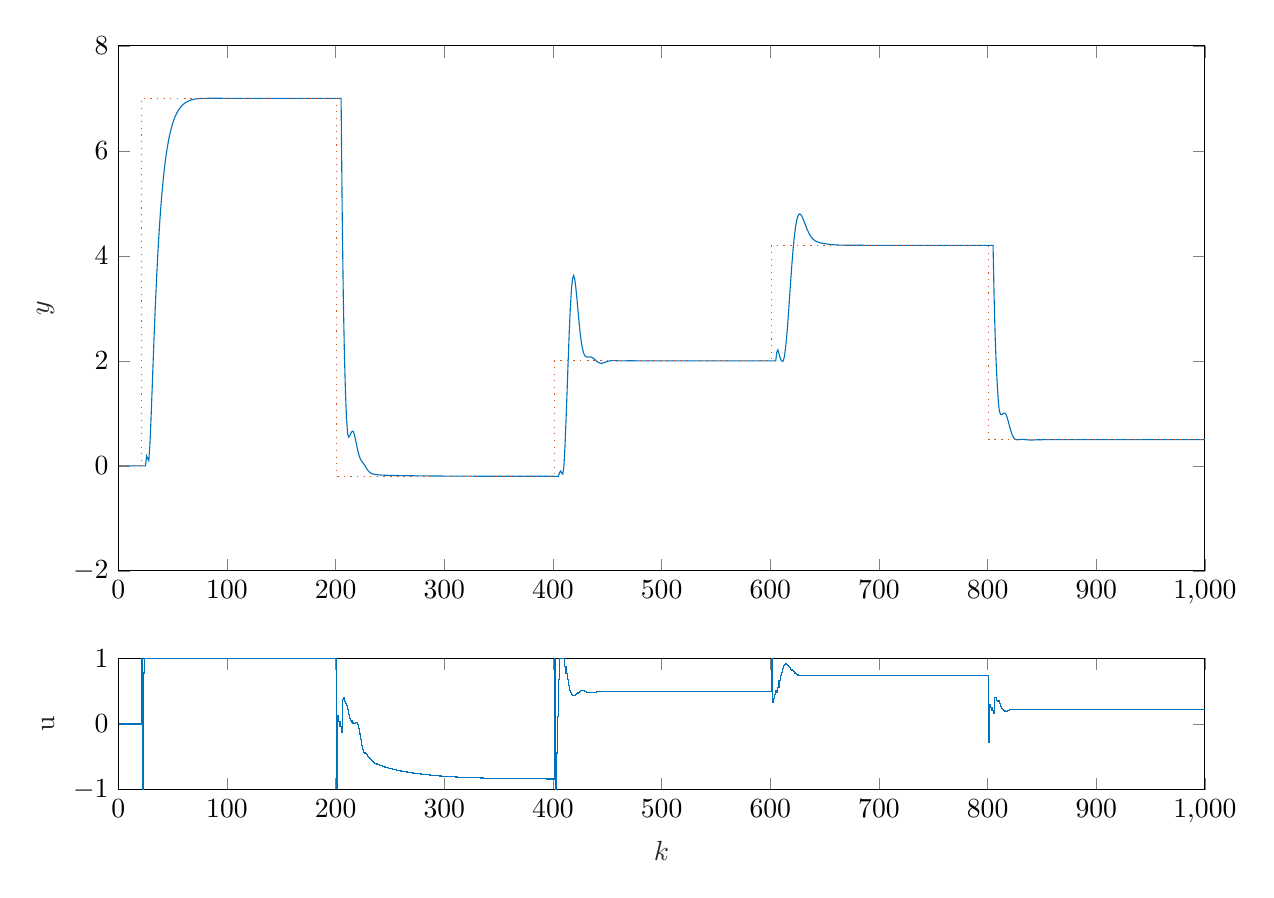
\begin{tikzpicture}

\begin{axis}[%
width=5.433in,
height=0.656in,
at={(0.854in,0.525in)},
scale only axis,
xmin=0,
xmax=1000,
xtick={0,100,200,300,400,500,600,700,800,900,1000},
xlabel style={font=\color{white!15!black}},
xlabel={$k$},
ymin=-1,
ymax=1,
ytick={-1,0,1},
ylabel style={font=\color{white!15!black}},
ylabel={u},
axis background/.style={fill=white}
]
\addplot[const plot, color=mycolor1, forget plot] table[row sep=crcr] {%
1	0\\
2	0\\
3	0\\
4	0\\
5	0\\
6	0\\
7	0\\
8	0\\
9	0\\
10	0\\
11	0\\
12	0\\
13	0\\
14	0\\
15	0\\
16	0\\
17	0\\
18	0\\
19	0\\
20	0\\
21	1\\
22	-1\\
23	0.777079448640233\\
24	1\\
25	1\\
26	1\\
27	1\\
28	1\\
29	1\\
30	1\\
31	1\\
32	1\\
33	1\\
34	1\\
35	1\\
36	1\\
37	1\\
38	1\\
39	1\\
40	1\\
41	1\\
42	1\\
43	1\\
44	1\\
45	1\\
46	1\\
47	1\\
48	1\\
49	1\\
50	1\\
51	1\\
52	1\\
53	1\\
54	1\\
55	1\\
56	1\\
57	0.999974756988591\\
58	0.999919868581213\\
59	0.999838983916182\\
60	0.999735303508606\\
61	0.999611634183505\\
62	0.999473315069462\\
63	0.999326734796187\\
64	0.999177544833026\\
65	0.999030529248285\\
66	0.998889793356824\\
67	0.998758565869549\\
68	0.998639042153589\\
69	0.99853248705045\\
70	0.998439402122901\\
71	0.998359654069727\\
72	0.998292605559378\\
73	0.998237263983106\\
74	0.99819241808692\\
75	0.998156747474242\\
76	0.998128910104128\\
77	0.998107610973227\\
78	0.998091650746616\\
79	0.998079955636249\\
80	0.998071592446154\\
81	0.998065772302312\\
82	0.99806184574559\\
83	0.998059291777395\\
84	0.998057703303697\\
85	0.998056770907671\\
86	0.998056266353475\\
87	0.998056026843379\\
88	0.998055940725246\\
89	0.998055935042656\\
90	0.998055965077637\\
91	0.998056005867722\\
92	0.998056045564539\\
93	0.99805608042679\\
94	0.998056111202473\\
95	0.998056140646494\\
96	0.99805617193067\\
97	0.998056207726112\\
98	0.998056249768168\\
99	0.998056298747281\\
100	0.998056354401947\\
101	0.998056415720258\\
102	0.998056481182986\\
103	0.998056549003331\\
104	0.998056617336118\\
105	0.998056684442652\\
106	0.998056748807083\\
107	0.998056809206576\\
108	0.998056864741511\\
109	0.9980569148338\\
110	0.998056959201936\\
111	0.998056997820878\\
112	0.998057030873838\\
113	0.998057058701669\\
114	0.998057081754132\\
115	0.998057100545989\\
116	0.998057115619643\\
117	0.998057127515141\\
118	0.998057136747541\\
119	0.998057143791172\\
120	0.998057149069934\\
121	0.998057152952651\\
122	0.998057155752381\\
123	0.998057157728679\\
124	0.998057159091872\\
125	0.998057160008545\\
126	0.998057160607609\\
127	0.99805716098643\\
128	0.998057161216674\\
129	0.998057161349636\\
130	0.9980571614209\\
131	0.998057161454286\\
132	0.99805716146509\\
133	0.998057161462656\\
134	0.998057161452346\\
135	0.998057161437009\\
136	0.998057161418027\\
137	0.99805716139602\\
138	0.998057161371297\\
139	0.99805716134412\\
140	0.998057161314827\\
141	0.998057161283877\\
142	0.998057161251835\\
143	0.99805716121933\\
144	0.998057161187011\\
145	0.998057161155499\\
146	0.998057161125344\\
147	0.998057161097003\\
148	0.998057161070823\\
149	0.998057161047038\\
150	0.998057161025769\\
151	0.998057161007043\\
152	0.998057160990801\\
153	0.998057160976918\\
154	0.998057160965222\\
155	0.998057160955505\\
156	0.998057160947545\\
157	0.998057160941117\\
158	0.998057160935998\\
159	0.998057160931979\\
160	0.998057160928868\\
161	0.998057160926496\\
162	0.998057160924715\\
163	0.998057160923398\\
164	0.99805716092244\\
165	0.998057160921755\\
166	0.998057160921274\\
167	0.998057160920942\\
168	0.998057160920718\\
169	0.998057160920571\\
170	0.998057160920477\\
171	0.99805716092042\\
172	0.998057160920387\\
173	0.998057160920371\\
174	0.998057160920365\\
175	0.998057160920367\\
176	0.998057160920373\\
177	0.998057160920383\\
178	0.998057160920394\\
179	0.998057160920408\\
180	0.998057160920423\\
181	0.998057160920438\\
182	0.998057160920453\\
183	0.998057160920469\\
184	0.998057160920484\\
185	0.998057160920499\\
186	0.998057160920513\\
187	0.998057160920527\\
188	0.998057160920539\\
189	0.998057160920551\\
190	0.998057160920561\\
191	0.99805716092057\\
192	0.998057160920578\\
193	0.998057160920586\\
194	0.998057160920591\\
195	0.998057160920596\\
196	0.998057160920601\\
197	0.998057160920604\\
198	0.998057160920606\\
199	0.998057160920608\\
200	0.998057160920609\\
201	-0.985572128652152\\
202	0.126816096562764\\
203	0.0429373642271242\\
204	-0.0409413681085153\\
205	-0.124820100444155\\
206	0.37995562088173\\
207	0.408036936431627\\
208	0.345482788975005\\
209	0.306929100147806\\
210	0.282737939425183\\
211	0.222076563643101\\
212	0.14064059203979\\
213	0.0844800816719967\\
214	0.0484182221393032\\
215	0.0222754966047122\\
216	0.00884800291271864\\
217	0.0103659155800627\\
218	0.0170277166916341\\
219	0.0213819870820107\\
220	-0.00701006973524907\\
221	-0.0670380225743896\\
222	-0.152367804644749\\
223	-0.241353506428831\\
224	-0.325642492648095\\
225	-0.392398115799697\\
226	-0.43275416009892\\
227	-0.453557696876287\\
228	-0.469572555429612\\
229	-0.488409698221654\\
230	-0.508738388245911\\
231	-0.528157383664355\\
232	-0.546117789716158\\
233	-0.562496448169804\\
234	-0.576680061578878\\
235	-0.588361839641252\\
236	-0.598046187462579\\
237	-0.606419994598625\\
238	-0.613907744929575\\
239	-0.620739861203896\\
240	-0.627110920848486\\
241	-0.633171848661922\\
242	-0.638981152106198\\
243	-0.644548222335822\\
244	-0.649885017863208\\
245	-0.655013511609266\\
246	-0.659953021697135\\
247	-0.664717994959586\\
248	-0.669323634314389\\
249	-0.673785395616186\\
250	-0.678115665962869\\
251	-0.682323162898578\\
252	-0.686414531322607\\
253	-0.690395387981388\\
254	-0.694270333913045\\
255	-0.698043128832601\\
256	-0.701717112315859\\
257	-0.70529544346072\\
258	-0.708781097021953\\
259	-0.712176833525245\\
260	-0.715485242565826\\
261	-0.718708781793243\\
262	-0.721849784432568\\
263	-0.724910465256208\\
264	-0.727892939552711\\
265	-0.730799242696669\\
266	-0.73363134040659\\
267	-0.736391134791311\\
268	-0.739080470432992\\
269	-0.741701139582087\\
270	-0.744254885335496\\
271	-0.746743403684363\\
272	-0.749168345563842\\
273	-0.751531318850787\\
274	-0.753833890031834\\
275	-0.756077585616936\\
276	-0.758263893462204\\
277	-0.760394264016395\\
278	-0.762470111439859\\
279	-0.764492814614709\\
280	-0.766463718091124\\
281	-0.768384132987381\\
282	-0.770255337844295\\
283	-0.772078579440019\\
284	-0.773855073575759\\
285	-0.775586005837381\\
286	-0.777272532333708\\
287	-0.778915780412881\\
288	-0.780516849359047\\
289	-0.78207681107099\\
290	-0.78359671072351\\
291	-0.785077567412303\\
292	-0.78652037478327\\
293	-0.787926101646936\\
294	-0.789295692578524\\
295	-0.790630068504101\\
296	-0.791930127273213\\
297	-0.793196744218391\\
298	-0.794430772701836\\
299	-0.795633044649593\\
300	-0.796804371073476\\
301	-0.797945542581044\\
302	-0.799057329873855\\
303	-0.800140484234269\\
304	-0.801195738001021\\
305	-0.802223805033815\\
306	-0.803225381167152\\
307	-0.804201144653621\\
308	-0.80515175659687\\
309	-0.806077861374468\\
310	-0.806980087050875\\
311	-0.807859045780711\\
312	-0.80871533420255\\
313	-0.809549533823416\\
314	-0.810362211394192\\
315	-0.811153919276129\\
316	-0.811925195798645\\
317	-0.812676565608609\\
318	-0.813408540011278\\
319	-0.814121617303092\\
320	-0.814816283096475\\
321	-0.815493010636847\\
322	-0.816152261111996\\
323	-0.816794483953993\\
324	-0.817420117133808\\
325	-0.818029587448795\\
326	-0.818623310803204\\
327	-0.819201692481876\\
328	-0.819765127417276\\
329	-0.820314000450021\\
330	-0.820848686583037\\
331	-0.821369551229511\\
332	-0.821876950454757\\
333	-0.822371231212162\\
334	-0.822852731573326\\
335	-0.823321780952541\\
336	-0.823778700325749\\
337	-0.824223802444083\\
338	-0.824657392042152\\
339	-0.825079766041158\\
340	-0.825491213746996\\
341	-0.825892017043438\\
342	-0.82628245058052\\
343	-0.826662781958253\\
344	-0.827033271905762\\
345	-0.827394174455963\\
346	-0.827745737115888\\
347	-0.828088201032759\\
348	-0.828421801155914\\
349	-0.828746766394681\\
350	-0.829063319772312\\
351	-0.829371678576046\\
352	-0.829672054503426\\
353	-0.829964653804927\\
354	-0.830249677423022\\
355	-0.830527321127736\\
356	-0.830797775648799\\
357	-0.831061226804469\\
358	-0.831317855627111\\
359	-0.831567838485613\\
360	-0.831811347204705\\
361	-0.832048549181273\\
362	-0.832279607497734\\
363	-0.832504681032538\\
364	-0.832723924567885\\
365	-0.832937488894704\\
366	-0.833145520914981\\
367	-0.833348163741491\\
368	-0.833545556794999\\
369	-0.833737835898997\\
370	-0.833925133372034\\
371	-0.834107578117702\\
372	-0.834285295712332\\
373	-0.834458408490466\\
374	-0.834627035628146\\
375	-0.834791293224088\\
376	-0.834951294378791\\
377	-0.835107149271624\\
378	-0.835258965235952\\
379	-0.835406846832344\\
380	-0.835550895919919\\
381	-0.83569121172586\\
382	-0.835827890913163\\
383	-0.835961027646653\\
384	-0.836090713657308\\
385	-0.836217038304944\\
386	-0.836340088639296\\
387	-0.836459949459532\\
388	-0.836576703372252\\
389	-0.836690430847993\\
390	-0.836801210276294\\
391	-0.836909118019346\\
392	-0.837014228464268\\
393	-0.837116614074046\\
394	-0.837216345437162\\
395	-0.837313491315949\\
396	-0.837408118693711\\
397	-0.837500292820629\\
398	-0.837590077258488\\
399	-0.837677533924262\\
400	-0.837762723132569\\
401	1\\
402	-1\\
403	-0.44156804945592\\
404	0.116865942499076\\
405	0.675301922962452\\
406	1\\
407	1\\
408	1\\
409	1\\
410	1\\
411	0.87029067980937\\
412	0.77004008297487\\
413	0.677775170399416\\
414	0.587584638821485\\
415	0.517703563591951\\
416	0.474180665007435\\
417	0.446023253431693\\
418	0.431282092467673\\
419	0.429848259074508\\
420	0.438846786161909\\
421	0.453026366095855\\
422	0.468851543413713\\
423	0.483947355976125\\
424	0.496561016196788\\
425	0.505016836808016\\
426	0.508826024424014\\
427	0.508514190348426\\
428	0.505042121797872\\
429	0.499504821579688\\
430	0.493100290490259\\
431	0.486935705719734\\
432	0.481832210080151\\
433	0.478283446733706\\
434	0.47649688404902\\
435	0.476423697121846\\
436	0.477800525505951\\
437	0.480215744664303\\
438	0.483205095209096\\
439	0.486324192010921\\
440	0.48919985693626\\
441	0.491563797846829\\
442	0.493266861404139\\
443	0.494271255057896\\
444	0.494629253769247\\
445	0.494456564296989\\
446	0.493904481596443\\
447	0.493133696062208\\
448	0.492292936920433\\
449	0.491504120892978\\
450	0.490853981754639\\
451	0.49039156862363\\
452	0.490130784982001\\
453	0.490056675345043\\
454	0.490133865286696\\
455	0.490315655022291\\
456	0.49055253082906\\
457	0.490799152203486\\
458	0.491019240362656\\
459	0.491188203174566\\
460	0.491293673108695\\
461	0.49133436027432\\
462	0.491317745720398\\
463	0.491257172282223\\
464	0.491168840187452\\
465	0.491069108502793\\
466	0.490972373322891\\
467	0.490889661434467\\
468	0.490827958295298\\
469	0.49079019315321\\
470	0.490775739102621\\
471	0.490781252754106\\
472	0.490801673761654\\
473	0.490831223344203\\
474	0.490864276103284\\
475	0.490896022928232\\
476	0.490922887189087\\
477	0.490942695899169\\
478	0.490954638131978\\
479	0.490959062715839\\
480	0.49095717598497\\
481	0.490950699493937\\
482	0.490941539380807\\
483	0.490931506172563\\
484	0.490922108926285\\
485	0.490914433007549\\
486	0.490909098279022\\
487	0.490906285113432\\
488	0.490905809925165\\
489	0.490907229749131\\
490	0.490909956274391\\
491	0.490913362884539\\
492	0.490916872774298\\
493	0.490920021232472\\
494	0.490922489962571\\
495	0.490924115304633\\
496	0.490924875096397\\
497	0.490924860554048\\
498	0.490924240028203\\
499	0.490923220998128\\
500	0.490922015482595\\
501	0.490920812471658\\
502	0.490919759303957\\
503	0.490918952363489\\
504	0.490918436214597\\
505	0.49091820942665\\
506	0.490918234883935\\
507	0.490918452298209\\
508	0.490918790867575\\
509	0.490919180460255\\
510	0.490919560244724\\
511	0.490919884246409\\
512	0.490920123811943\\
513	0.490920267354705\\
514	0.490920318014351\\
515	0.49092028998544\\
516	0.490920204270626\\
517	0.490920084519289\\
518	0.490919953455696\\
519	0.490919830215252\\
520	0.490919728722888\\
521	0.490919657086937\\
522	0.490919617860099\\
523	0.490919608942858\\
524	0.490919624873558\\
525	0.49091965825726\\
526	0.49091970112285\\
527	0.490919746053363\\
528	0.490919786997356\\
529	0.490919819729572\\
530	0.490919841980347\\
531	0.490919853290547\\
532	0.490919854670838\\
533	0.490919848151303\\
534	0.490919836302228\\
535	0.490919821792662\\
536	0.490919807033915\\
537	0.490919793934059\\
538	0.490919783769797\\
539	0.490919777165898\\
540	0.490919774161032\\
541	0.490919774332681\\
542	0.490919776952358\\
543	0.490919781144953\\
544	0.490919786031268\\
545	0.490919790839538\\
546	0.490919794978778\\
547	0.490919798073169\\
548	0.490919799961781\\
549	0.490919800671309\\
550	0.490919800371243\\
551	0.490919799320968\\
552	0.490919797817247\\
553	0.4909197961486\\
554	0.490919794560797\\
555	0.490919793235355\\
556	0.490919792280861\\
557	0.490919791735393\\
558	0.49091979157727\\
559	0.490919791740955\\
560	0.490919792134957\\
561	0.490919792659053\\
562	0.490919793218805\\
563	0.490919793736146\\
564	0.490919794155573\\
565	0.490919794446142\\
566	0.490919794599929\\
567	0.49091979462794\\
568	0.490919794554547\\
569	0.490919794411473\\
570	0.490919794232181\\
571	0.490919794047279\\
572	0.490919793881309\\
573	0.490919793750998\\
574	0.490919793664888\\
575	0.490919793624063\\
576	0.490919793623669\\
577	0.490919793654834\\
578	0.490919793706672\\
579	0.490919793768098\\
580	0.490919793829268\\
581	0.490919793882541\\
582	0.490919793922956\\
583	0.490919793948265\\
584	0.490919793958614\\
585	0.490919793956\\
586	0.490919793943608\\
587	0.49091979392515\\
588	0.490919793904281\\
589	0.490919793884153\\
590	0.490919793867131\\
591	0.490919793854665\\
592	0.490919793847314\\
593	0.49091979384487\\
594	0.490919793846556\\
595	0.490919793851246\\
596	0.490919793857687\\
597	0.49091979386468\\
598	0.490919793871225\\
599	0.490919793876597\\
600	0.49091979388038\\
601	1\\
602	0.32443526218716\\
603	0.384490916263153\\
604	0.444546570338235\\
605	0.504602224412828\\
606	0.479902031966788\\
607	0.560252209930387\\
608	0.660337445238745\\
609	0.734503674180614\\
610	0.789129197559165\\
611	0.847158039668116\\
612	0.891459926409861\\
613	0.913790630119566\\
614	0.918716779434344\\
615	0.912872668832726\\
616	0.898507509065755\\
617	0.879093224711876\\
618	0.857223272888725\\
619	0.835045869449342\\
620	0.813928839687799\\
621	0.79484539711511\\
622	0.778429243564633\\
623	0.764979957575268\\
624	0.754517584816151\\
625	0.746863616817442\\
626	0.741701822406631\\
627	0.73862454850847\\
628	0.737183229433468\\
629	0.736935075365151\\
630	0.73747711199443\\
631	0.738467523557685\\
632	0.73963688016498\\
633	0.740790030140889\\
634	0.741800234283628\\
635	0.742598512336238\\
636	0.743160986960848\\
637	0.743496088378031\\
638	0.743632867854553\\
639	0.743611228328897\\
640	0.743474406909304\\
641	0.743263662245865\\
642	0.743014917057095\\
643	0.742757017365599\\
644	0.742511234000555\\
645	0.742291639297258\\
646	0.742106034986299\\
647	0.741957166232455\\
648	0.74184401774289\\
649	0.741763046224274\\
650	0.741709256356165\\
651	0.741677071706982\\
652	0.741660986218626\\
653	0.741656006413364\\
654	0.741657910351673\\
655	0.741663357832701\\
656	0.741669888911066\\
657	0.74167584616168\\
658	0.741680251772117\\
659	0.741682664738916\\
660	0.741683037185346\\
661	0.741681582829926\\
662	0.741678665382523\\
663	0.741674710371058\\
664	0.741670140681172\\
665	0.741665333877979\\
666	0.741660598050081\\
667	0.741656162306762\\
668	0.74165217799341\\
669	0.741648726998892\\
670	0.741645834063812\\
671	0.741643480639333\\
672	0.741641618500951\\
673	0.74164018192702\\
674	0.741639097769169\\
675	0.7416382931529\\
676	0.741637700848706\\
677	0.74163726255482\\
678	0.74163693044678\\
679	0.741636667393926\\
680	0.741636446237002\\
681	0.741636248481053\\
682	0.741636062698534\\
683	0.741635882870358\\
684	0.741635706826335\\
685	0.741635534886709\\
686	0.741635368756596\\
687	0.741635210686478\\
688	0.741635062884392\\
689	0.741634927147946\\
690	0.741634804675212\\
691	0.74163469601106\\
692	0.741634601087566\\
693	0.741634519322332\\
694	0.741634449745207\\
695	0.741634391131098\\
696	0.741634342123392\\
697	0.741634301338543\\
698	0.741634267447278\\
699	0.741634239231582\\
700	0.741634215619244\\
701	0.741634195699272\\
702	0.741634178722273\\
703	0.74163416409002\\
704	0.741634151338109\\
705	0.741634140115058\\
706	0.741634130160495\\
707	0.74163412128436\\
708	0.74163411334839\\
709	0.741634106250565\\
710	0.741634099912761\\
711	0.741634094271484\\
712	0.741634089271385\\
713	0.741634084861096\\
714	0.741634080990884\\
715	0.741634077611657\\
716	0.741634074674862\\
717	0.741634072132939\\
718	0.741634069940016\\
719	0.741634068052654\\
720	0.741634066430506\\
721	0.741634065036803\\
722	0.741634063838639\\
723	0.741634062807064\\
724	0.741634061916997\\
725	0.741634061147005\\
726	0.741634060478986\\
727	0.741634059897788\\
728	0.741634059390811\\
729	0.741634058947611\\
730	0.741634058559525\\
731	0.741634058219346\\
732	0.741634057921026\\
733	0.741634057659448\\
734	0.741634057430225\\
735	0.741634057229555\\
736	0.741634057054101\\
737	0.741634056900912\\
738	0.741634056767356\\
739	0.741634056651078\\
740	0.741634056549968\\
741	0.741634056462138\\
742	0.741634056385901\\
743	0.741634056319757\\
744	0.74163405626238\\
745	0.741634056212602\\
746	0.741634056169402\\
747	0.74163405613189\\
748	0.741634056099295\\
749	0.741634056070951\\
750	0.741634056046283\\
751	0.7416340560248\\
752	0.741634056006078\\
753	0.741634055989755\\
754	0.741634055975518\\
755	0.741634055963098\\
756	0.741634055952264\\
757	0.741634055942812\\
758	0.74163405593457\\
759	0.741634055927384\\
760	0.741634055921122\\
761	0.741634055915667\\
762	0.741634055910917\\
763	0.741634055906782\\
764	0.741634055903184\\
765	0.741634055900054\\
766	0.741634055897331\\
767	0.741634055894962\\
768	0.741634055892902\\
769	0.74163405589111\\
770	0.741634055889551\\
771	0.741634055888194\\
772	0.741634055887013\\
773	0.741634055885985\\
774	0.741634055885091\\
775	0.741634055884312\\
776	0.741634055883633\\
777	0.741634055883042\\
778	0.741634055882527\\
779	0.741634055882078\\
780	0.741634055881687\\
781	0.741634055881347\\
782	0.74163405588105\\
783	0.741634055880792\\
784	0.741634055880567\\
785	0.741634055880371\\
786	0.741634055880201\\
787	0.741634055880052\\
788	0.741634055879923\\
789	0.741634055879811\\
790	0.741634055879713\\
791	0.741634055879628\\
792	0.741634055879554\\
793	0.741634055879489\\
794	0.741634055879433\\
795	0.741634055879383\\
796	0.741634055879341\\
797	0.741634055879304\\
798	0.741634055879271\\
799	0.741634055879243\\
800	0.741634055879219\\
801	-0.277730995706806\\
802	0.293912953361952\\
803	0.250808604800565\\
804	0.20770425623918\\
805	0.164599907677797\\
806	0.400157868140731\\
807	0.398192592540311\\
808	0.362555300741236\\
809	0.349435137157962\\
810	0.350457391589542\\
811	0.311575970769444\\
812	0.267249758341746\\
813	0.23907896773247\\
814	0.220095236386955\\
815	0.203144867737084\\
816	0.194490777001951\\
817	0.19600253072838\\
818	0.202072878105758\\
819	0.208907555361978\\
820	0.21586872518717\\
821	0.221823616901418\\
822	0.225466032341115\\
823	0.226769980773417\\
824	0.226458751076497\\
825	0.225126191277442\\
826	0.223237741994321\\
827	0.221296935317951\\
828	0.219705843978717\\
829	0.218643306246685\\
830	0.218127511025383\\
831	0.218096992488183\\
832	0.21843241021697\\
833	0.218980956473233\\
834	0.219599854519904\\
835	0.220183276067646\\
836	0.220665360703216\\
837	0.221016295769419\\
838	0.22123706413746\\
839	0.221349941867567\\
840	0.221387007367316\\
841	0.22138118140216\\
842	0.221360686700546\\
843	0.221345910192933\\
844	0.221348383939536\\
845	0.221371726697404\\
846	0.221413737410214\\
847	0.221468757029213\\
848	0.221529821727671\\
849	0.221590366996404\\
850	0.22164532152166\\
851	0.221691572540071\\
852	0.221727932522124\\
853	0.221754785242467\\
854	0.221773572395416\\
855	0.221786256504013\\
856	0.221794862270972\\
857	0.221801151830274\\
858	0.221806445769372\\
859	0.221811573208588\\
860	0.221816918601073\\
861	0.221822526553626\\
862	0.221828228017697\\
863	0.221833759463333\\
864	0.221838857197812\\
865	0.221843318944637\\
866	0.221847032879587\\
867	0.221849979867675\\
868	0.221852217409548\\
869	0.22185385416652\\
870	0.221855022656566\\
871	0.221855855564454\\
872	0.221856468716344\\
873	0.221856951618055\\
874	0.221857364848791\\
875	0.221857742640618\\
876	0.221858098610495\\
877	0.221858432715096\\
878	0.221858737902353\\
879	0.22185900547089\\
880	0.221859228683047\\
881	0.221859404617672\\
882	0.221859534550394\\
883	0.221859623304369\\
884	0.221859678044015\\
885	0.221859706923414\\
886	0.221859717889611\\
887	0.221859717814385\\
888	0.221859712012897\\
889	0.22185970411989\\
890	0.221859696240188\\
891	0.221859689268235\\
892	0.22185968327493\\
893	0.221859677880083\\
894	0.221859672556611\\
895	0.22185966684086\\
896	0.221859660447107\\
897	0.221859653300733\\
898	0.221859645513355\\
899	0.221859637325164\\
900	0.221859629036825\\
901	0.221859620947539\\
902	0.221859613309158\\
903	0.221859606300058\\
904	0.221859600017687\\
905	0.221859594485687\\
906	0.221859589670164\\
907	0.221859585499762\\
908	0.221859581885177\\
909	0.221859578735178\\
910	0.221859575967693\\
911	0.221859573515794\\
912	0.221859571329293\\
913	0.221859569373169\\
914	0.221859567624166\\
915	0.221859566066767\\
916	0.221859564689457\\
917	0.221859563481822\\
918	0.22185956243271\\
919	0.221859561529422\\
920	0.22185956075772\\
921	0.221859560102367\\
922	0.221859559547927\\
923	0.221859559079569\\
924	0.221859558683724\\
925	0.221859558348515\\
926	0.22185955806393\\
927	0.221859557821777\\
928	0.221859557615492\\
929	0.221859557439852\\
930	0.221859557290665\\
931	0.221859557164485\\
932	0.221859557058383\\
933	0.221859556969778\\
934	0.221859556896335\\
935	0.221859556835914\\
936	0.221859556786552\\
937	0.221859556746473\\
938	0.221859556714093\\
939	0.221859556688037\\
940	0.221859556667135\\
941	0.221859556650412\\
942	0.221859556637076\\
943	0.221859556626486\\
944	0.221859556618134\\
945	0.221859556611613\\
946	0.221859556606596\\
947	0.221859556602813\\
948	0.221859556600043\\
949	0.221859556598095\\
950	0.22185955659681\\
951	0.221859556596047\\
952	0.221859556595689\\
953	0.221859556595635\\
954	0.221859556595804\\
955	0.221859556596128\\
956	0.221859556596554\\
957	0.221859556597044\\
958	0.221859556597567\\
959	0.221859556598101\\
960	0.221859556598632\\
961	0.221859556599148\\
962	0.221859556599644\\
963	0.221859556600114\\
964	0.221859556600556\\
965	0.221859556600968\\
966	0.221859556601349\\
967	0.221859556601699\\
968	0.221859556602018\\
969	0.221859556602308\\
970	0.221859556602568\\
971	0.221859556602802\\
972	0.22185955660301\\
973	0.221859556603195\\
974	0.221859556603359\\
975	0.221859556603503\\
976	0.221859556603629\\
977	0.22185955660374\\
978	0.221859556603837\\
979	0.221859556603922\\
980	0.221859556603995\\
981	0.221859556604059\\
982	0.221859556604114\\
983	0.221859556604162\\
984	0.221859556604204\\
985	0.221859556604239\\
986	0.22185955660427\\
987	0.221859556604296\\
988	0.221859556604318\\
989	0.221859556604337\\
990	0.221859556604353\\
991	0.221859556604366\\
992	0.221859556604378\\
993	0.221859556604387\\
994	0.221859556604395\\
995	0.221859556604402\\
996	0.221859556604408\\
997	0.221859556604412\\
998	0.221859556604416\\
999	0.221859556604419\\
1000	0.221859556604422\\
};
\end{axis}

\begin{axis}[%
width=5.433in,
height=2.625in,
at={(0.854in,1.619in)},
scale only axis,
xmin=0,
xmax=1000,
xtick={0,100,200,300,400,500,600,700,800,900,1000},
ymin=-2,
ymax=8,
ytick={-2,0,2,4,6,8},
ylabel style={font=\color{white!15!black}},
ylabel={$y$},
axis background/.style={fill=white}
]
\addplot [color=mycolor1, forget plot]
  table[row sep=crcr]{%
1	0\\
2	0\\
3	0\\
4	0\\
5	0\\
6	0\\
7	0\\
8	0\\
9	0\\
10	0\\
11	0\\
12	0\\
13	0\\
14	0\\
15	0\\
16	0\\
17	0\\
18	0\\
19	0\\
20	0\\
21	0\\
22	0\\
23	0\\
24	0\\
25	0\\
26	0.187021166666667\\
27	0.1388412867175\\
28	0.0985523229521002\\
29	0.378463327376529\\
30	0.849284660283429\\
31	1.39883483390368\\
32	1.96363189679148\\
33	2.50917220020059\\
34	3.01803694011572\\
35	3.48273842732905\\
36	3.90143395402948\\
37	4.27537255985532\\
38	4.60738720809724\\
39	4.90101605548333\\
40	5.16000090271522\\
41	5.38801056227388\\
42	5.58849725934977\\
43	5.76463074850641\\
44	5.91927695818501\\
45	6.0550013534964\\
46	6.17408528327832\\
47	6.27854844117594\\
48	6.37017349034512\\
49	6.4505306457979\\
50	6.5210010431221\\
51	6.58279832940326\\
52	6.63698826241639\\
53	6.68450630080679\\
54	6.72617327341197\\
55	6.76270926768289\\
56	6.79474589793668\\
57	6.82283711743353\\
58	6.84746873205929\\
59	6.86906676244619\\
60	6.88800478842648\\
61	6.90461039634414\\
62	6.91916039158136\\
63	6.931885440819\\
64	6.9429813077052\\
65	6.95261757737569\\
66	6.96094334018374\\
67	6.96809220415809\\
68	6.97418654146288\\
69	6.97934015122329\\
70	6.98365962085278\\
71	6.98724498587077\\
72	6.99018992998059\\
73	6.99258163438919\\
74	6.99450046596333\\
75	6.99601967985063\\
76	6.99720522326866\\
77	6.99811567689984\\
78	6.99880235453011\\
79	6.99930956197221\\
80	6.99967499494027\\
81	6.9999302449689\\
82	7.00010138044716\\
83	7.00020957033255\\
84	7.00027172030306\\
85	7.00030109557658\\
86	7.00030791032977\\
87	7.00029986931551\\
88	7.00028265248608\\
89	7.00026033806373\\
90	7.00023576336874\\
91	7.0002108256866\\
92	7.00018672756816\\
93	7.00016417231401\\
94	7.00014351610775\\
95	7.00012488345126\\
96	7.00010825234831\\
97	7.0000935152016\\
98	7.00008052073677\\
99	7.00006910152858\\
100	7.00005909094658\\
101	7.00005033260947\\
102	7.000042684771\\
103	7.00003602147585\\
104	7.00003023182973\\
105	7.00002521832394\\
106	7.00002089483652\\
107	7.00001718469071\\
108	7.00001401897499\\
109	7.00001133520767\\
110	7.00000907635032\\
111	7.00000719012815\\
112	7.00000562859374\\
113	7.00000434786466\\
114	7.00000330797026\\
115	7.00000247275319\\
116	7.00000180978441\\
117	7.00000129026312\\
118	7.00000088888516\\
119	7.00000058367295\\
120	7.0000003557674\\
121	7.0000001891875\\
122	7.0000000705661\\
123	6.9999999888718\\
124	6.999999935127\\
125	6.99999990213106\\
126	6.99999988419621\\
127	6.99999987690206\\
128	6.99999987687271\\
129	6.9999998815789\\
130	6.99999988916588\\
131	6.99999989830686\\
132	6.99999990808043\\
133	6.99999991787028\\
134	6.99999992728456\\
135	6.9999999360925\\
136	6.99999994417556\\
137	6.99999995149066\\
138	6.99999995804315\\
139	6.99999996386757\\
140	6.99999996901431\\
141	6.99999997354073\\
142	6.99999997750563\\
143	6.99999998096591\\
144	6.99999998397487\\
145	6.99999998658149\\
146	6.99999998883033\\
147	6.99999999076172\\
148	6.99999999241216\\
149	6.99999999381467\\
150	6.99999999499924\\
151	6.99999999599304\\
152	6.99999999682076\\
153	6.99999999750477\\
154	6.99999999806523\\
155	6.99999999852032\\
156	6.99999999888623\\
157	6.99999999917732\\
158	6.99999999940624\\
159	6.99999999958399\\
160	6.99999999972007\\
161	6.99999999982258\\
162	6.99999999989837\\
163	6.99999999995315\\
164	6.99999999999165\\
165	7.0000000000177\\
166	7.00000000003442\\
167	7.00000000004424\\
168	7.00000000004911\\
169	7.0000000000505\\
170	7.00000000004955\\
171	7.00000000004709\\
172	7.00000000004373\\
173	7.00000000003992\\
174	7.00000000003595\\
175	7.00000000003203\\
176	7.00000000002829\\
177	7.0000000000248\\
178	7.00000000002161\\
179	7.00000000001872\\
180	7.00000000001613\\
181	7.00000000001383\\
182	7.00000000001181\\
183	7.00000000001003\\
184	7.00000000000848\\
185	7.00000000000713\\
186	7.00000000000596\\
187	7.00000000000496\\
188	7.0000000000041\\
189	7.00000000000336\\
190	7.00000000000274\\
191	7.00000000000222\\
192	7.00000000000178\\
193	7.00000000000141\\
194	7.00000000000111\\
195	7.00000000000086\\
196	7.00000000000066\\
197	7.0000000000005\\
198	7.00000000000037\\
199	7.00000000000027\\
200	7.0000000000002\\
201	7.00000000000014\\
202	7.0000000000001\\
203	7.00000000000006\\
204	7.00000000000004\\
205	7.00000000000002\\
206	4.8633547666178\\
207	3.25877503965815\\
208	2.17426882188505\\
209	1.42137030951934\\
210	0.895123794698473\\
211	0.614020737914612\\
212	0.546688791774948\\
213	0.572367083499868\\
214	0.617987383008621\\
215	0.654902514364715\\
216	0.659614343690815\\
217	0.614295504369336\\
218	0.52902546608446\\
219	0.426866768770966\\
220	0.326318156762095\\
221	0.238662683744204\\
222	0.169593310400037\\
223	0.119842011530036\\
224	0.086417869997192\\
225	0.0610173120470905\\
226	0.0338751474513076\\
227	0.000880919138794149\\
228	-0.0348628656973631\\
229	-0.0681548153536816\\
230	-0.0960981262454368\\
231	-0.11805888495113\\
232	-0.134354857336892\\
233	-0.145779182790138\\
234	-0.153561076763044\\
235	-0.159005866347574\\
236	-0.163052836073883\\
237	-0.166232684082532\\
238	-0.168839113976228\\
239	-0.17104502454859\\
240	-0.172936452247933\\
241	-0.174547095128778\\
242	-0.175905043775234\\
243	-0.177049887016277\\
244	-0.178024574303069\\
245	-0.178866720122729\\
246	-0.179607705558952\\
247	-0.180273447067283\\
248	-0.180883375903584\\
249	-0.181450517328144\\
250	-0.181983359727747\\
251	-0.182487795470644\\
252	-0.18296812517923\\
253	-0.183427520509366\\
254	-0.183868446117639\\
255	-0.18429295463145\\
256	-0.184702775465915\\
257	-0.185099318731722\\
258	-0.185483709086705\\
259	-0.18585684677577\\
260	-0.186219455042442\\
261	-0.186572115242726\\
262	-0.186915301684332\\
263	-0.187249413600455\\
264	-0.187574797391993\\
265	-0.18789175981955\\
266	-0.188200577095371\\
267	-0.188501501825166\\
268	-0.188794767796924\\
269	-0.189080593154084\\
270	-0.189359182890561\\
271	-0.189630731056929\\
272	-0.189895422559906\\
273	-0.190153434530944\\
274	-0.190404937388983\\
275	-0.190650095685169\\
276	-0.190889068750761\\
277	-0.191122011176016\\
278	-0.191349073173855\\
279	-0.191570400869537\\
280	-0.191786136535384\\
281	-0.191996418782461\\
282	-0.192201382721233\\
283	-0.19240116010024\\
284	-0.19259587942728\\
285	-0.192785666075982\\
286	-0.192970642380871\\
287	-0.193150927723624\\
288	-0.193326638612402\\
289	-0.193497888755597\\
290	-0.193664789131173\\
291	-0.193827448052526\\
292	-0.193985971231526\\
293	-0.194140461839171\\
294	-0.194291020564213\\
295	-0.194437745670014\\
296	-0.194580733049844\\
297	-0.19472007628075\\
298	-0.194855866676137\\
299	-0.194988193337128\\
300	-0.195117143202803\\
301	-0.195242801099352\\
302	-0.195365249788204\\
303	-0.195484570013159\\
304	-0.19560084054656\\
305	-0.195714138234526\\
306	-0.195824538041269\\
307	-0.19593211309251\\
308	-0.196036934718021\\
309	-0.196139072493297\\
310	-0.196238594280374\\
311	-0.196335566267814\\
312	-0.196430053009867\\
313	-0.19652211746481\\
314	-0.196611821032497\\
315	-0.196699223591118\\
316	-0.196784383533178\\
317	-0.196867357800717\\
318	-0.196948201919777\\
319	-0.197026970034126\\
320	-0.197103714938256\\
321	-0.197178488109667\\
322	-0.197251339740442\\
323	-0.197322318768132\\
324	-0.197391472905958\\
325	-0.197458848672351\\
326	-0.197524491419822\\
327	-0.197588445363199\\
328	-0.197650753607227\\
329	-0.197711458173538\\
330	-0.197770600027024\\
331	-0.197828219101595\\
332	-0.197884354325369\\
333	-0.197939043645265\\
334	-0.197992324051043\\
335	-0.198044231598791\\
336	-0.19809480143386\\
337	-0.198144067813274\\
338	-0.19819206412762\\
339	-0.198238822922415\\
340	-0.19828437591899\\
341	-0.198328754034869\\
342	-0.198371987403676\\
343	-0.198414105394571\\
344	-0.198455136631225\\
345	-0.198495109010345\\
346	-0.198534049719755\\
347	-0.198571985256058\\
348	-0.19860894144186\\
349	-0.198644943442593\\
350	-0.198680015782931\\
351	-0.198714182362807\\
352	-0.198747466473056\\
353	-0.198779890810664\\
354	-0.198811477493664\\
355	-0.19884224807566\\
356	-0.198872223560003\\
357	-0.198901424413622\\
358	-0.19892987058052\\
359	-0.198957581494937\\
360	-0.19898457609419\\
361	-0.199010872831209\\
362	-0.199036489686754\\
363	-0.199061444181335\\
364	-0.199085753386847\\
365	-0.199109433937907\\
366	-0.199132502042919\\
367	-0.199154973494865\\
368	-0.199176863681825\\
369	-0.199198187597244\\
370	-0.199218959849938\\
371	-0.199239194673856\\
372	-0.199258905937596\\
373	-0.199278107153688\\
374	-0.199296811487644\\
375	-0.199315031766785\\
376	-0.199332780488843\\
377	-0.199350069830351\\
378	-0.199366911654828\\
379	-0.199383317520747\\
380	-0.199399298689321\\
381	-0.199414866132075\\
382	-0.199430030538244\\
383	-0.199444802321974\\
384	-0.19945919162935\\
385	-0.199473208345242\\
386	-0.19948686209998\\
387	-0.199500162275865\\
388	-0.199513118013509\\
389	-0.199525738218018\\
390	-0.199538031565025\\
391	-0.199550006506558\\
392	-0.199561671276771\\
393	-0.199573033897526\\
394	-0.199584102183832\\
395	-0.199594883749147\\
396	-0.19960538601055\\
397	-0.199615616193776\\
398	-0.199625581338123\\
399	-0.199635288301244\\
400	-0.199644743763802\\
401	-0.199653954234024\\
402	-0.199662926052121\\
403	-0.199671665394611\\
404	-0.199680178278526\\
405	-0.199688470565506\\
406	-0.131390354147964\\
407	-0.0995347356606516\\
408	-0.133789122779729\\
409	-0.158729349998457\\
410	-0.0234233746311477\\
411	0.340195222546204\\
412	0.857393306638562\\
413	1.4312175330292\\
414	2.00735646984629\\
415	2.55681070675096\\
416	3.02260048245524\\
417	3.3624663296551\\
418	3.56332275754663\\
419	3.62355174177398\\
420	3.55855929889653\\
421	3.40199210797878\\
422	3.19084642829787\\
423	2.95836189022545\\
424	2.73212494522853\\
425	2.5320357705301\\
426	2.36893783987727\\
427	2.24598141097379\\
428	2.16100797894591\\
429	2.10861812642392\\
430	2.08149106536272\\
431	2.07158853104932\\
432	2.07129707730668\\
433	2.07423916674174\\
434	2.07569798154362\\
435	2.07278618972598\\
436	2.06438892539732\\
437	2.05087405646835\\
438	2.03364900591141\\
439	2.01468129852222\\
440	1.99605920194264\\
441	1.97963572096519\\
442	1.9667829753734\\
443	1.95827366835689\\
444	1.95427725785602\\
445	1.95444092681645\\
446	1.95802350765771\\
447	1.96405341295407\\
448	1.97148439715042\\
449	1.97932908785638\\
450	1.98675852191104\\
451	1.99316305201007\\
452	1.99817526850875\\
453	2.00165986461842\\
454	2.00367846892444\\
455	2.00443886617076\\
456	2.00423792246346\\
457	2.00340640239875\\
458	2.0022619903868\\
459	2.00107448813967\\
460	2.00004477420402\\
461	1.99929704643247\\
462	1.99888231849336\\
463	1.9987901833096\\
464	1.99896549082652\\
465	1.99932673356307\\
466	1.99978344944608\\
467	2.00025068356521\\
468	2.00065936005501\\
469	2.00096218598805\\
470	2.0011353539436\\
471	2.00117677734969\\
472	2.00110186507299\\
473	2.00093792828818\\
474	2.00071824284431\\
475	2.0004766068774\\
476	2.00024298429308\\
477	2.00004055581753\\
478	1.99988424897665\\
479	1.99978061431867\\
480	1.99972877316872\\
481	1.99972208646786\\
482	1.99975017965966\\
483	1.99980099339376\\
484	1.99986259864706\\
485	1.99992460148722\\
486	1.99997905227172\\
487	2.0000208546803\\
488	2.00004773347572\\
489	2.00005986207277\\
490	2.00005927126085\\
491	2.00004916104318\\
492	2.00003322276411\\
493	2.00001505373653\\
494	1.99999771682215\\
495	1.9999834676516\\
496	1.9999736461382\\
497	1.99996870908383\\
498	1.99996836812805\\
499	1.99997179201178\\
500	1.99997783317124\\
501	1.99998524451388\\
502	1.99999286106341\\
503	1.99999973122005\\
504	2.00000519213017\\
505	2.00000889194042\\
506	2.00001076780744\\
507	2.00001099216373\\
508	2.00000990099037\\
509	2.00000791708854\\
510	2.00000547911236\\
511	2.00000298403223\\
512	2.00000074732037\\
513	1.99999898197649\\
514	1.99999779489682\\
515	1.99999719723903\\
516	1.99999712441364\\
517	1.9999974610853\\
518	1.9999980669546\\
519	1.99999879992442\\
520	1.99999953433126\\
521	2.00000017305242\\
522	2.00000065332992\\
523	2.0000009469755\\
524	2.00000105617872\\
525	2.0000010064215\\
526	2.00000083803299\\
527	2.00000059774949\\
528	2.00000033134136\\
529	2.00000007799913\\
530	1.99999986679656\\
531	1.99999971521652\\
532	1.99999962946892\\
533	1.99999960616426\\
534	1.99999963483209\\
535	1.99999970078024\\
536	1.99999978785907\\
537	1.99999988080319\\
538	1.99999996694879\\
539	2.0000000372476\\
540	2.00000008660483\\
541	2.00000011364711\\
542	2.00000012007508\\
543	2.00000010977335\\
544	2.00000008784296\\
545	2.00000005969481\\
546	2.00000003030445\\
547	2.00000000368607\\
548	1.99999998260332\\
549	1.99999996850105\\
550	1.99999996161753\\
551	1.99999996122331\\
552	1.99999996592869\\
553	1.99999997400594\\
554	1.99999998368259\\
555	1.99999999337527\\
556	2.00000000184792\\
557	2.0000000082911\\
558	2.00000001233007\\
559	2.00000001397618\\
560	2.00000001354036\\
561	2.00000001152797\\
562	2.00000000853229\\
563	2.00000000514051\\
564	2.00000000186113\\
565	1.9999999990773\\
566	1.9999999970262\\
567	1.99999999580135\\
568	1.99999999537242\\
569	1.99999999561632\\
570	1.99999999635299\\
571	1.9999999973806\\
572	1.99999999850559\\
573	1.99999999956511\\
574	2.0000000004407\\
575	2.00000000106326\\
576	2.00000000141085\\
577	2.00000000150096\\
578	2.00000000137961\\
579	2.00000000110922\\
580	2.00000000075713\\
581	2.00000000038606\\
582	2.00000000004719\\
583	1.99999999977633\\
584	1.99999999959277\\
585	1.99999999950053\\
586	1.9999999994912\\
587	1.99999999954779\\
588	1.99999999964873\\
589	1.9999999997716\\
590	1.99999999989617\\
591	2.00000000000643\\
592	2.0000000000917\\
593	2.00000000014679\\
594	2.00000000017142\\
595	2.00000000016923\\
596	2.0000000001464\\
597	2.00000000011035\\
598	2.0000000000685\\
599	2.00000000002739\\
600	1.99999999999201\\
601	1.99999999996552\\
602	1.99999999994928\\
603	1.99999999994305\\
604	1.99999999994539\\
605	1.99999999995411\\
606	2.16535210391806\\
607	2.20785355300273\\
608	2.13768210100682\\
609	2.05766139419394\\
610	2.01332510816144\\
611	1.98784354180062\\
612	2.0024900990987\\
613	2.08420905982949\\
614	2.23521313640301\\
615	2.4426053134102\\
616	2.69534145994986\\
617	2.98185245389257\\
618	3.28553014371451\\
619	3.58783535079096\\
620	3.87268088232784\\
621	4.12757084550001\\
622	4.34393587612204\\
623	4.51714971149208\\
624	4.64617430156756\\
625	4.73290012755612\\
626	4.78140373309324\\
627	4.79723946648906\\
628	4.786766528068\\
629	4.75653963347827\\
630	4.71280971964581\\
631	4.66115821198678\\
632	4.60626402067155\\
633	4.55179431775181\\
634	4.50040274092343\\
635	4.45380983728985\\
636	4.41293697046803\\
637	4.37806731324081\\
638	4.34901234223337\\
639	4.32526765173068\\
640	4.30614756388274\\
641	4.29089325653849\\
642	4.27875325147807\\
643	4.26903796236528\\
644	4.2611517832446\\
645	4.25460709882875\\
646	4.24902479927316\\
647	4.24412559580557\\
648	4.23971585796422\\
649	4.23567097689754\\
650	4.23191850818811\\
651	4.22842263882706\\
652	4.22517090603772\\
653	4.22216359533993\\
654	4.21940586783281\\
655	4.21690240623447\\
656	4.21465421168238\\
657	4.21265710981392\\
658	4.21090151479636\\
659	4.20937303418312\\
660	4.20805355845933\\
661	4.20692255271305\\
662	4.20595834325218\\
663	4.20513926172167\\
664	4.20444456883278\\
665	4.20385512705994\\
666	4.20335382627183\\
667	4.20292578917976\\
668	4.20255839640883\\
669	4.20224117598732\\
670	4.20196560122162\\
671	4.20172483624021\\
672	4.20151346162754\\
673	4.20132720486213\\
674	4.20116269270219\\
675	4.2010172358795\\
676	4.20088865083695\\
677	4.20077511892424\\
678	4.20067508042827\\
679	4.20058715893098\\
680	4.20051011056321\\
681	4.20044279254075\\
682	4.20038414571123\\
683	4.20033318651373\\
684	4.20028900459422\\
685	4.20025076320279\\
686	4.20021770033359\\
687	4.20018912929898\\
688	4.20016443802438\\
689	4.20014308680378\\
690	4.20012460457228\\
691	4.20010858395054\\
692	4.20009467541655\\
693	4.20008258098741\\
694	4.20007204776969\\
695	4.20006286168113\\
696	4.20005484157529\\
697	4.20004783392593\\
698	4.20004170815869\\
699	4.2000363526583\\
700	4.20003167143371\\
701	4.20002758139014\\
702	4.20002401013736\\
703	4.20002089425306\\
704	4.20001817791934\\
705	4.20001581185469\\
706	4.20001375247269\\
707	4.20001196120935\\
708	4.20001040397219\\
709	4.20000905067547\\
710	4.20000787483522\\
711	4.20000685320641\\
712	4.20000596545064\\
713	4.20000519382801\\
714	4.20000452290989\\
715	4.20000393931158\\
716	4.20000343144506\\
717	4.2000029892922\\
718	4.20000260419916\\
719	4.20000226869191\\
720	4.2000019763128\\
721	4.20000172147717\\
722	4.20000149934897\\
723	4.20000130573378\\
724	4.2000011369874\\
725	4.20000098993833\\
726	4.20000086182216\\
727	4.20000075022618\\
728	4.20000065304251\\
729	4.20000056842844\\
730	4.20000049477261\\
731	4.20000043066605\\
732	4.20000037487721\\
733	4.20000032633024\\
734	4.200000284086\\
735	4.20000024732543\\
736	4.20000021533481\\
737	4.20000018749273\\
738	4.20000016325856\\
739	4.20000014216225\\
740	4.2000001237953\\
741	4.20000010780281\\
742	4.20000009387644\\
743	4.20000008174834\\
744	4.20000007118574\\
745	4.20000006198631\\
746	4.20000005397409\\
747	4.200000046996\\
748	4.20000004091879\\
749	4.20000003562642\\
750	4.20000003101781\\
751	4.20000002700486\\
752	4.20000002351082\\
753	4.20000002046875\\
754	4.20000001782031\\
755	4.20000001551466\\
756	4.20000001350747\\
757	4.20000001176014\\
758	4.200000010239\\
759	4.20000000891477\\
760	4.20000000776194\\
761	4.20000000675828\\
762	4.20000000588447\\
763	4.20000000512368\\
764	4.20000000446127\\
765	4.20000000388451\\
766	4.20000000338231\\
767	4.20000000294502\\
768	4.20000000256425\\
769	4.20000000223269\\
770	4.20000000194399\\
771	4.20000000169261\\
772	4.20000000147371\\
773	4.20000000128312\\
774	4.20000000111717\\
775	4.20000000097268\\
776	4.20000000084687\\
777	4.20000000073734\\
778	4.20000000064197\\
779	4.20000000055894\\
780	4.20000000048665\\
781	4.20000000042372\\
782	4.20000000036892\\
783	4.20000000032121\\
784	4.20000000027967\\
785	4.20000000024351\\
786	4.20000000021202\\
787	4.2000000001846\\
788	4.20000000016073\\
789	4.20000000013995\\
790	4.20000000012185\\
791	4.20000000010609\\
792	4.20000000009237\\
793	4.20000000008043\\
794	4.20000000007003\\
795	4.20000000006097\\
796	4.20000000005309\\
797	4.20000000004622\\
798	4.20000000004025\\
799	4.20000000003504\\
800	4.20000000003051\\
801	4.20000000002657\\
802	4.20000000002313\\
803	4.20000000002014\\
804	4.20000000001753\\
805	4.20000000001527\\
806	3.18853649948835\\
807	2.41750871723688\\
808	1.88603532140039\\
809	1.49413301847749\\
810	1.18591453054643\\
811	1.02541294455221\\
812	0.979560291410048\\
813	0.979072136289898\\
814	0.990190312105741\\
815	1.00429766481337\\
816	1.00353269682982\\
817	0.973499153526838\\
818	0.91728017090572\\
819	0.845601316409727\\
820	0.767457754442684\\
821	0.691207277267788\\
822	0.624689124786553\\
823	0.572514033538043\\
824	0.535508452823641\\
825	0.512255979417978\\
826	0.500211745707722\\
827	0.49616111682514\\
828	0.496822201367655\\
829	0.499475203724383\\
830	0.502218965257793\\
831	0.503936965000835\\
832	0.504191675286621\\
833	0.503073034688514\\
834	0.500988265977766\\
835	0.498456932566959\\
836	0.495966484495248\\
837	0.493888032091729\\
838	0.492438138633824\\
839	0.491680651186525\\
840	0.491558203375242\\
841	0.491936361714641\\
842	0.492647003258496\\
843	0.493524251585141\\
844	0.494429594345462\\
845	0.495264874142537\\
846	0.495974512440533\\
847	0.496540126396523\\
848	0.496970909582217\\
849	0.497292648321966\\
850	0.497537616670911\\
851	0.49773679106874\\
852	0.497914943540163\\
853	0.498088478374031\\
854	0.498265467845462\\
855	0.498447155507003\\
856	0.498630178203349\\
857	0.498808876687201\\
858	0.498977259260467\\
859	0.499130387163952\\
860	0.49926512516232\\
861	0.49938032918727\\
862	0.499476618267585\\
863	0.499555902984043\\
864	0.499620829351099\\
865	0.49967426072516\\
866	0.499718874714512\\
867	0.499756907723043\\
868	0.499790043977121\\
869	0.49981942218925\\
870	0.499845721563309\\
871	0.499869287619525\\
872	0.499890264244547\\
873	0.499908708149091\\
874	0.499924672615666\\
875	0.499938256900293\\
876	0.499949624685893\\
877	0.499958999158507\\
878	0.499966643797596\\
879	0.499972837435043\\
880	0.499977850303217\\
881	0.499981925396991\\
882	0.499985267111649\\
883	0.499988037184518\\
884	0.49999035665759\\
885	0.499992311915496\\
886	0.499993962742701\\
887	0.499995350626073\\
888	0.499996506028541\\
889	0.499997453920003\\
890	0.499998217356736\\
891	0.499998819281038\\
892	0.499999282943326\\
893	0.499999631438026\\
894	0.49999988682244\\
895	0.500000069193956\\
896	0.500000195974592\\
897	0.500000281524992\\
898	0.500000337104495\\
899	0.500000371120826\\
900	0.500000389574277\\
901	0.500000396592393\\
902	0.500000394963924\\
903	0.50000038660581\\
904	0.500000372925984\\
905	0.500000355071361\\
906	0.500000334070658\\
907	0.500000310894233\\
908	0.500000286458136\\
909	0.500000261598574\\
910	0.500000237038143\\
911	0.500000213358384\\
912	0.500000190986382\\
913	0.5000001701973\\
914	0.500000151130635\\
915	0.5000001338157\\
916	0.500000118201186\\
917	0.500000104184177\\
918	0.500000091635209\\
919	0.500000080417474\\
920	0.500000070399619\\
921	0.500000061462697\\
922	0.500000053502464\\
923	0.500000046428538\\
924	0.500000040161831\\
925	0.500000034631482\\
926	0.500000029772087\\
927	0.500000025521704\\
928	0.500000021820757\\
929	0.500000018611756\\
930	0.5000000158396\\
931	0.500000013452201\\
932	0.50000001140118\\
933	0.500000009642434\\
934	0.500000008136489\\
935	0.500000006848575\\
936	0.500000005748458\\
937	0.500000004810084\\
938	0.5000000040111\\
939	0.500000003332334\\
940	0.500000002757286\\
941	0.500000002271679\\
942	0.500000001863082\\
943	0.500000001520613\\
944	0.500000001234719\\
945	0.500000000997015\\
946	0.500000000800158\\
947	0.500000000637758\\
948	0.500000000504285\\
949	0.500000000394999\\
950	0.500000000305866\\
951	0.500000000233476\\
952	0.500000000174969\\
953	0.500000000127951\\
954	0.500000000090426\\
955	0.500000000060728\\
956	0.500000000037467\\
957	0.500000000019481\\
958	0.500000000005795\\
959	0.499999999995596\\
960	0.499999999988199\\
961	0.499999999983033\\
962	0.499999999979627\\
963	0.499999999977587\\
964	0.499999999976596\\
965	0.499999999976394\\
966	0.499999999976773\\
967	0.499999999977569\\
968	0.499999999978651\\
969	0.49999999997992\\
970	0.499999999981298\\
971	0.499999999982725\\
972	0.49999999998416\\
973	0.499999999985567\\
974	0.499999999986925\\
975	0.499999999988216\\
976	0.49999999998943\\
977	0.499999999990559\\
978	0.499999999991602\\
979	0.499999999992557\\
980	0.499999999993426\\
981	0.499999999994212\\
982	0.49999999999492\\
983	0.499999999995553\\
984	0.499999999996119\\
985	0.499999999996621\\
986	0.499999999997066\\
987	0.499999999997459\\
988	0.499999999997804\\
989	0.499999999998107\\
990	0.499999999998373\\
991	0.499999999998604\\
992	0.499999999998806\\
993	0.499999999998981\\
994	0.499999999999133\\
995	0.499999999999264\\
996	0.499999999999376\\
997	0.499999999999473\\
998	0.499999999999556\\
999	0.499999999999627\\
1000	0.499999999999688\\
};
\addplot[const plot, color=mycolor2, dotted, forget plot] table[row sep=crcr] {%
1	0\\
2	0\\
3	0\\
4	0\\
5	0\\
6	0\\
7	0\\
8	0\\
9	0\\
10	0\\
11	0\\
12	0\\
13	0\\
14	0\\
15	0\\
16	0\\
17	0\\
18	0\\
19	0\\
20	0\\
21	7\\
22	7\\
23	7\\
24	7\\
25	7\\
26	7\\
27	7\\
28	7\\
29	7\\
30	7\\
31	7\\
32	7\\
33	7\\
34	7\\
35	7\\
36	7\\
37	7\\
38	7\\
39	7\\
40	7\\
41	7\\
42	7\\
43	7\\
44	7\\
45	7\\
46	7\\
47	7\\
48	7\\
49	7\\
50	7\\
51	7\\
52	7\\
53	7\\
54	7\\
55	7\\
56	7\\
57	7\\
58	7\\
59	7\\
60	7\\
61	7\\
62	7\\
63	7\\
64	7\\
65	7\\
66	7\\
67	7\\
68	7\\
69	7\\
70	7\\
71	7\\
72	7\\
73	7\\
74	7\\
75	7\\
76	7\\
77	7\\
78	7\\
79	7\\
80	7\\
81	7\\
82	7\\
83	7\\
84	7\\
85	7\\
86	7\\
87	7\\
88	7\\
89	7\\
90	7\\
91	7\\
92	7\\
93	7\\
94	7\\
95	7\\
96	7\\
97	7\\
98	7\\
99	7\\
100	7\\
101	7\\
102	7\\
103	7\\
104	7\\
105	7\\
106	7\\
107	7\\
108	7\\
109	7\\
110	7\\
111	7\\
112	7\\
113	7\\
114	7\\
115	7\\
116	7\\
117	7\\
118	7\\
119	7\\
120	7\\
121	7\\
122	7\\
123	7\\
124	7\\
125	7\\
126	7\\
127	7\\
128	7\\
129	7\\
130	7\\
131	7\\
132	7\\
133	7\\
134	7\\
135	7\\
136	7\\
137	7\\
138	7\\
139	7\\
140	7\\
141	7\\
142	7\\
143	7\\
144	7\\
145	7\\
146	7\\
147	7\\
148	7\\
149	7\\
150	7\\
151	7\\
152	7\\
153	7\\
154	7\\
155	7\\
156	7\\
157	7\\
158	7\\
159	7\\
160	7\\
161	7\\
162	7\\
163	7\\
164	7\\
165	7\\
166	7\\
167	7\\
168	7\\
169	7\\
170	7\\
171	7\\
172	7\\
173	7\\
174	7\\
175	7\\
176	7\\
177	7\\
178	7\\
179	7\\
180	7\\
181	7\\
182	7\\
183	7\\
184	7\\
185	7\\
186	7\\
187	7\\
188	7\\
189	7\\
190	7\\
191	7\\
192	7\\
193	7\\
194	7\\
195	7\\
196	7\\
197	7\\
198	7\\
199	7\\
200	7\\
201	-0.2\\
202	-0.2\\
203	-0.2\\
204	-0.2\\
205	-0.2\\
206	-0.2\\
207	-0.2\\
208	-0.2\\
209	-0.2\\
210	-0.2\\
211	-0.2\\
212	-0.2\\
213	-0.2\\
214	-0.2\\
215	-0.2\\
216	-0.2\\
217	-0.2\\
218	-0.2\\
219	-0.2\\
220	-0.2\\
221	-0.2\\
222	-0.2\\
223	-0.2\\
224	-0.2\\
225	-0.2\\
226	-0.2\\
227	-0.2\\
228	-0.2\\
229	-0.2\\
230	-0.2\\
231	-0.2\\
232	-0.2\\
233	-0.2\\
234	-0.2\\
235	-0.2\\
236	-0.2\\
237	-0.2\\
238	-0.2\\
239	-0.2\\
240	-0.2\\
241	-0.2\\
242	-0.2\\
243	-0.2\\
244	-0.2\\
245	-0.2\\
246	-0.2\\
247	-0.2\\
248	-0.2\\
249	-0.2\\
250	-0.2\\
251	-0.2\\
252	-0.2\\
253	-0.2\\
254	-0.2\\
255	-0.2\\
256	-0.2\\
257	-0.2\\
258	-0.2\\
259	-0.2\\
260	-0.2\\
261	-0.2\\
262	-0.2\\
263	-0.2\\
264	-0.2\\
265	-0.2\\
266	-0.2\\
267	-0.2\\
268	-0.2\\
269	-0.2\\
270	-0.2\\
271	-0.2\\
272	-0.2\\
273	-0.2\\
274	-0.2\\
275	-0.2\\
276	-0.2\\
277	-0.2\\
278	-0.2\\
279	-0.2\\
280	-0.2\\
281	-0.2\\
282	-0.2\\
283	-0.2\\
284	-0.2\\
285	-0.2\\
286	-0.2\\
287	-0.2\\
288	-0.2\\
289	-0.2\\
290	-0.2\\
291	-0.2\\
292	-0.2\\
293	-0.2\\
294	-0.2\\
295	-0.2\\
296	-0.2\\
297	-0.2\\
298	-0.2\\
299	-0.2\\
300	-0.2\\
301	-0.2\\
302	-0.2\\
303	-0.2\\
304	-0.2\\
305	-0.2\\
306	-0.2\\
307	-0.2\\
308	-0.2\\
309	-0.2\\
310	-0.2\\
311	-0.2\\
312	-0.2\\
313	-0.2\\
314	-0.2\\
315	-0.2\\
316	-0.2\\
317	-0.2\\
318	-0.2\\
319	-0.2\\
320	-0.2\\
321	-0.2\\
322	-0.2\\
323	-0.2\\
324	-0.2\\
325	-0.2\\
326	-0.2\\
327	-0.2\\
328	-0.2\\
329	-0.2\\
330	-0.2\\
331	-0.2\\
332	-0.2\\
333	-0.2\\
334	-0.2\\
335	-0.2\\
336	-0.2\\
337	-0.2\\
338	-0.2\\
339	-0.2\\
340	-0.2\\
341	-0.2\\
342	-0.2\\
343	-0.2\\
344	-0.2\\
345	-0.2\\
346	-0.2\\
347	-0.2\\
348	-0.2\\
349	-0.2\\
350	-0.2\\
351	-0.2\\
352	-0.2\\
353	-0.2\\
354	-0.2\\
355	-0.2\\
356	-0.2\\
357	-0.2\\
358	-0.2\\
359	-0.2\\
360	-0.2\\
361	-0.2\\
362	-0.2\\
363	-0.2\\
364	-0.2\\
365	-0.2\\
366	-0.2\\
367	-0.2\\
368	-0.2\\
369	-0.2\\
370	-0.2\\
371	-0.2\\
372	-0.2\\
373	-0.2\\
374	-0.2\\
375	-0.2\\
376	-0.2\\
377	-0.2\\
378	-0.2\\
379	-0.2\\
380	-0.2\\
381	-0.2\\
382	-0.2\\
383	-0.2\\
384	-0.2\\
385	-0.2\\
386	-0.2\\
387	-0.2\\
388	-0.2\\
389	-0.2\\
390	-0.2\\
391	-0.2\\
392	-0.2\\
393	-0.2\\
394	-0.2\\
395	-0.2\\
396	-0.2\\
397	-0.2\\
398	-0.2\\
399	-0.2\\
400	-0.2\\
401	2\\
402	2\\
403	2\\
404	2\\
405	2\\
406	2\\
407	2\\
408	2\\
409	2\\
410	2\\
411	2\\
412	2\\
413	2\\
414	2\\
415	2\\
416	2\\
417	2\\
418	2\\
419	2\\
420	2\\
421	2\\
422	2\\
423	2\\
424	2\\
425	2\\
426	2\\
427	2\\
428	2\\
429	2\\
430	2\\
431	2\\
432	2\\
433	2\\
434	2\\
435	2\\
436	2\\
437	2\\
438	2\\
439	2\\
440	2\\
441	2\\
442	2\\
443	2\\
444	2\\
445	2\\
446	2\\
447	2\\
448	2\\
449	2\\
450	2\\
451	2\\
452	2\\
453	2\\
454	2\\
455	2\\
456	2\\
457	2\\
458	2\\
459	2\\
460	2\\
461	2\\
462	2\\
463	2\\
464	2\\
465	2\\
466	2\\
467	2\\
468	2\\
469	2\\
470	2\\
471	2\\
472	2\\
473	2\\
474	2\\
475	2\\
476	2\\
477	2\\
478	2\\
479	2\\
480	2\\
481	2\\
482	2\\
483	2\\
484	2\\
485	2\\
486	2\\
487	2\\
488	2\\
489	2\\
490	2\\
491	2\\
492	2\\
493	2\\
494	2\\
495	2\\
496	2\\
497	2\\
498	2\\
499	2\\
500	2\\
501	2\\
502	2\\
503	2\\
504	2\\
505	2\\
506	2\\
507	2\\
508	2\\
509	2\\
510	2\\
511	2\\
512	2\\
513	2\\
514	2\\
515	2\\
516	2\\
517	2\\
518	2\\
519	2\\
520	2\\
521	2\\
522	2\\
523	2\\
524	2\\
525	2\\
526	2\\
527	2\\
528	2\\
529	2\\
530	2\\
531	2\\
532	2\\
533	2\\
534	2\\
535	2\\
536	2\\
537	2\\
538	2\\
539	2\\
540	2\\
541	2\\
542	2\\
543	2\\
544	2\\
545	2\\
546	2\\
547	2\\
548	2\\
549	2\\
550	2\\
551	2\\
552	2\\
553	2\\
554	2\\
555	2\\
556	2\\
557	2\\
558	2\\
559	2\\
560	2\\
561	2\\
562	2\\
563	2\\
564	2\\
565	2\\
566	2\\
567	2\\
568	2\\
569	2\\
570	2\\
571	2\\
572	2\\
573	2\\
574	2\\
575	2\\
576	2\\
577	2\\
578	2\\
579	2\\
580	2\\
581	2\\
582	2\\
583	2\\
584	2\\
585	2\\
586	2\\
587	2\\
588	2\\
589	2\\
590	2\\
591	2\\
592	2\\
593	2\\
594	2\\
595	2\\
596	2\\
597	2\\
598	2\\
599	2\\
600	2\\
601	4.2\\
602	4.2\\
603	4.2\\
604	4.2\\
605	4.2\\
606	4.2\\
607	4.2\\
608	4.2\\
609	4.2\\
610	4.2\\
611	4.2\\
612	4.2\\
613	4.2\\
614	4.2\\
615	4.2\\
616	4.2\\
617	4.2\\
618	4.2\\
619	4.2\\
620	4.2\\
621	4.2\\
622	4.2\\
623	4.2\\
624	4.2\\
625	4.2\\
626	4.2\\
627	4.2\\
628	4.2\\
629	4.2\\
630	4.2\\
631	4.2\\
632	4.2\\
633	4.2\\
634	4.2\\
635	4.2\\
636	4.2\\
637	4.2\\
638	4.2\\
639	4.2\\
640	4.2\\
641	4.2\\
642	4.2\\
643	4.2\\
644	4.2\\
645	4.2\\
646	4.2\\
647	4.2\\
648	4.2\\
649	4.2\\
650	4.2\\
651	4.2\\
652	4.2\\
653	4.2\\
654	4.2\\
655	4.2\\
656	4.2\\
657	4.2\\
658	4.2\\
659	4.2\\
660	4.2\\
661	4.2\\
662	4.2\\
663	4.2\\
664	4.2\\
665	4.2\\
666	4.2\\
667	4.2\\
668	4.2\\
669	4.2\\
670	4.2\\
671	4.2\\
672	4.2\\
673	4.2\\
674	4.2\\
675	4.2\\
676	4.2\\
677	4.2\\
678	4.2\\
679	4.2\\
680	4.2\\
681	4.2\\
682	4.2\\
683	4.2\\
684	4.2\\
685	4.2\\
686	4.2\\
687	4.2\\
688	4.2\\
689	4.2\\
690	4.2\\
691	4.2\\
692	4.2\\
693	4.2\\
694	4.2\\
695	4.2\\
696	4.2\\
697	4.2\\
698	4.2\\
699	4.2\\
700	4.2\\
701	4.2\\
702	4.2\\
703	4.2\\
704	4.2\\
705	4.2\\
706	4.2\\
707	4.2\\
708	4.2\\
709	4.2\\
710	4.2\\
711	4.2\\
712	4.2\\
713	4.2\\
714	4.2\\
715	4.2\\
716	4.2\\
717	4.2\\
718	4.2\\
719	4.2\\
720	4.2\\
721	4.2\\
722	4.2\\
723	4.2\\
724	4.2\\
725	4.2\\
726	4.2\\
727	4.2\\
728	4.2\\
729	4.2\\
730	4.2\\
731	4.2\\
732	4.2\\
733	4.2\\
734	4.2\\
735	4.2\\
736	4.2\\
737	4.2\\
738	4.2\\
739	4.2\\
740	4.2\\
741	4.2\\
742	4.2\\
743	4.2\\
744	4.2\\
745	4.2\\
746	4.2\\
747	4.2\\
748	4.2\\
749	4.2\\
750	4.2\\
751	4.2\\
752	4.2\\
753	4.2\\
754	4.2\\
755	4.2\\
756	4.2\\
757	4.2\\
758	4.2\\
759	4.2\\
760	4.2\\
761	4.2\\
762	4.2\\
763	4.2\\
764	4.2\\
765	4.2\\
766	4.2\\
767	4.2\\
768	4.2\\
769	4.2\\
770	4.2\\
771	4.2\\
772	4.2\\
773	4.2\\
774	4.2\\
775	4.2\\
776	4.2\\
777	4.2\\
778	4.2\\
779	4.2\\
780	4.2\\
781	4.2\\
782	4.2\\
783	4.2\\
784	4.2\\
785	4.2\\
786	4.2\\
787	4.2\\
788	4.2\\
789	4.2\\
790	4.2\\
791	4.2\\
792	4.2\\
793	4.2\\
794	4.2\\
795	4.2\\
796	4.2\\
797	4.2\\
798	4.2\\
799	4.2\\
800	4.2\\
801	0.5\\
802	0.5\\
803	0.5\\
804	0.5\\
805	0.5\\
806	0.5\\
807	0.5\\
808	0.5\\
809	0.5\\
810	0.5\\
811	0.5\\
812	0.5\\
813	0.5\\
814	0.5\\
815	0.5\\
816	0.5\\
817	0.5\\
818	0.5\\
819	0.5\\
820	0.5\\
821	0.5\\
822	0.5\\
823	0.5\\
824	0.5\\
825	0.5\\
826	0.5\\
827	0.5\\
828	0.5\\
829	0.5\\
830	0.5\\
831	0.5\\
832	0.5\\
833	0.5\\
834	0.5\\
835	0.5\\
836	0.5\\
837	0.5\\
838	0.5\\
839	0.5\\
840	0.5\\
841	0.5\\
842	0.5\\
843	0.5\\
844	0.5\\
845	0.5\\
846	0.5\\
847	0.5\\
848	0.5\\
849	0.5\\
850	0.5\\
851	0.5\\
852	0.5\\
853	0.5\\
854	0.5\\
855	0.5\\
856	0.5\\
857	0.5\\
858	0.5\\
859	0.5\\
860	0.5\\
861	0.5\\
862	0.5\\
863	0.5\\
864	0.5\\
865	0.5\\
866	0.5\\
867	0.5\\
868	0.5\\
869	0.5\\
870	0.5\\
871	0.5\\
872	0.5\\
873	0.5\\
874	0.5\\
875	0.5\\
876	0.5\\
877	0.5\\
878	0.5\\
879	0.5\\
880	0.5\\
881	0.5\\
882	0.5\\
883	0.5\\
884	0.5\\
885	0.5\\
886	0.5\\
887	0.5\\
888	0.5\\
889	0.5\\
890	0.5\\
891	0.5\\
892	0.5\\
893	0.5\\
894	0.5\\
895	0.5\\
896	0.5\\
897	0.5\\
898	0.5\\
899	0.5\\
900	0.5\\
901	0.5\\
902	0.5\\
903	0.5\\
904	0.5\\
905	0.5\\
906	0.5\\
907	0.5\\
908	0.5\\
909	0.5\\
910	0.5\\
911	0.5\\
912	0.5\\
913	0.5\\
914	0.5\\
915	0.5\\
916	0.5\\
917	0.5\\
918	0.5\\
919	0.5\\
920	0.5\\
921	0.5\\
922	0.5\\
923	0.5\\
924	0.5\\
925	0.5\\
926	0.5\\
927	0.5\\
928	0.5\\
929	0.5\\
930	0.5\\
931	0.5\\
932	0.5\\
933	0.5\\
934	0.5\\
935	0.5\\
936	0.5\\
937	0.5\\
938	0.5\\
939	0.5\\
940	0.5\\
941	0.5\\
942	0.5\\
943	0.5\\
944	0.5\\
945	0.5\\
946	0.5\\
947	0.5\\
948	0.5\\
949	0.5\\
950	0.5\\
951	0.5\\
952	0.5\\
953	0.5\\
954	0.5\\
955	0.5\\
956	0.5\\
957	0.5\\
958	0.5\\
959	0.5\\
960	0.5\\
961	0.5\\
962	0.5\\
963	0.5\\
964	0.5\\
965	0.5\\
966	0.5\\
967	0.5\\
968	0.5\\
969	0.5\\
970	0.5\\
971	0.5\\
972	0.5\\
973	0.5\\
974	0.5\\
975	0.5\\
976	0.5\\
977	0.5\\
978	0.5\\
979	0.5\\
980	0.5\\
981	0.5\\
982	0.5\\
983	0.5\\
984	0.5\\
985	0.5\\
986	0.5\\
987	0.5\\
988	0.5\\
989	0.5\\
990	0.5\\
991	0.5\\
992	0.5\\
993	0.5\\
994	0.5\\
995	0.5\\
996	0.5\\
997	0.5\\
998	0.5\\
999	0.5\\
1000	0.5\\
};
\end{axis}
\end{tikzpicture}%
\caption{Symulacja modelu z rozmytym PID o trzech regulatorach. \\Błąd $ E=\num{1154,3} $}
\label{Z5b}
\end{figure}

\begin{figure}[ht]
\centering
% This file was created by matlab2tikz.
%
%The latest updates can be retrieved from
%  http://www.mathworks.com/matlabcentral/fileexchange/22022-matlab2tikz-matlab2tikz
%where you can also make suggestions and rate matlab2tikz.
%
ERR 1151.1
\definecolor{mycolor1}{rgb}{0.00000,0.44700,0.74100}%
\definecolor{mycolor2}{rgb}{0.85000,0.32500,0.09800}%
%
\begin{tikzpicture}

\begin{axis}[%
width=6.833in,
height=0.656in,
at={(0.854in,0.525in)},
scale only axis,
xmin=0,
xmax=1000,
xtick={0,100,200,300,400,500,600,700,800,900,1000},
xlabel style={font=\color{white!15!black}},
xlabel={k},
ymin=-1,
ymax=1,
ytick={-1,0,1},
ylabel style={font=\color{white!15!black}},
ylabel={u},
axis background/.style={fill=white}
]
\addplot[const plot, color=mycolor1, forget plot] table[row sep=crcr] {%
1	0\\
2	0\\
3	0\\
4	0\\
5	0\\
6	0\\
7	0\\
8	0\\
9	0\\
10	0\\
11	0\\
12	0\\
13	0\\
14	0\\
15	0\\
16	0\\
17	0\\
18	0\\
19	0\\
20	0\\
21	1\\
22	-1\\
23	1\\
24	1\\
25	1\\
26	1\\
27	1\\
28	1\\
29	1\\
30	1\\
31	1\\
32	1\\
33	1\\
34	1\\
35	1\\
36	1\\
37	1\\
38	1\\
39	1\\
40	1\\
41	1\\
42	1\\
43	1\\
44	1\\
45	1\\
46	1\\
47	1\\
48	1\\
49	1\\
50	1\\
51	1\\
52	1\\
53	1\\
54	1\\
55	1\\
56	1\\
57	0.999967792005714\\
58	0.999906795895747\\
59	0.999820555438343\\
60	0.999712178671646\\
61	0.999584391282136\\
62	0.999443255915826\\
63	0.999295235256106\\
64	0.999145755154132\\
65	0.998999427336996\\
66	0.99886022102646\\
67	0.99873116336803\\
68	0.99861422443403\\
69	0.998510479276465\\
70	0.998420275299083\\
71	0.998343349901601\\
72	0.998278965190922\\
73	0.998226060518648\\
74	0.998183384626228\\
75	0.998149598985531\\
76	0.998123361053089\\
77	0.998103389018131\\
78	0.998088506067676\\
79	0.998077666388698\\
80	0.998069967274796\\
81	0.998064650610117\\
82	0.998061096249721\\
83	0.998058809908799\\
84	0.998057407959561\\
85	0.998056600937481\\
86	0.998056177051968\\
87	0.998055986650705\\
88	0.998055928266632\\
89	0.998055936576084\\
90	0.998055972370206\\
91	0.99805601448927\\
92	0.998056053565099\\
93	0.998056087350562\\
94	0.998056117384697\\
95	0.998056146739094\\
96	0.998056178605744\\
97	0.99805621551174\\
98	0.998056258977744\\
99	0.998056309470734\\
100	0.998056366534156\\
101	0.998056429008229\\
102	0.998056495278829\\
103	0.998056563514537\\
104	0.99805663186818\\
105	0.998056698631723\\
106	0.998056762342214\\
107	0.998056821842335\\
108	0.99805687630244\\
109	0.998056925212531\\
110	0.998056968352791\\
111	0.998057005750648\\
112	0.998057037631186\\
113	0.998057064366288\\
114	0.998057086426513\\
115	0.998057104338338\\
116	0.998057118648279\\
117	0.998057129894479\\
118	0.998057138585644\\
119	0.998057145186737\\
120	0.998057150110521\\
121	0.998057153713927\\
122	0.998057156298162\\
123	0.998057158111547\\
124	0.99805715935417\\
125	0.998057160183601\\
126	0.998057160721043\\
127	0.998057161057456\\
128	0.99805716125933\\
129	0.998057161373884\\
130	0.998057161433582\\
131	0.998057161459933\\
132	0.998057161466573\\
133	0.998057161461697\\
134	0.998057161449913\\
135	0.998057161433603\\
136	0.998057161413883\\
137	0.998057161391242\\
138	0.998057161365943\\
139	0.998057161338247\\
140	0.998057161308516\\
141	0.998057161277233\\
142	0.998057161244983\\
143	0.998057161212409\\
144	0.99805716118016\\
145	0.998057161148847\\
146	0.998057161119006\\
147	0.998057161091072\\
148	0.998057161065367\\
149	0.998057161042101\\
150	0.998057161021373\\
151	0.998057161003188\\
152	0.99805716098747\\
153	0.998057160974081\\
154	0.99805716096284\\
155	0.998057160953533\\
156	0.998057160945936\\
157	0.998057160939821\\
158	0.998057160934969\\
159	0.998057160931174\\
160	0.998057160928248\\
161	0.998057160926025\\
162	0.998057160924363\\
163	0.998057160923139\\
164	0.998057160922252\\
165	0.998057160921621\\
166	0.998057160921179\\
167	0.998057160920877\\
168	0.998057160920675\\
169	0.998057160920542\\
170	0.998057160920458\\
171	0.998057160920407\\
172	0.99805716092038\\
173	0.998057160920366\\
174	0.998057160920363\\
175	0.998057160920366\\
176	0.998057160920374\\
177	0.998057160920384\\
178	0.998057160920396\\
179	0.99805716092041\\
180	0.998057160920425\\
181	0.99805716092044\\
182	0.998057160920455\\
183	0.998057160920471\\
184	0.998057160920487\\
185	0.998057160920502\\
186	0.998057160920516\\
187	0.99805716092053\\
188	0.998057160920542\\
189	0.998057160920553\\
190	0.998057160920562\\
191	0.998057160920571\\
192	0.998057160920579\\
193	0.998057160920585\\
194	0.998057160920591\\
195	0.998057160920596\\
196	0.9980571609206\\
197	0.998057160920604\\
198	0.998057160920607\\
199	0.998057160920609\\
200	0.998057160920611\\
201	-0.98557212865215\\
202	0.126816096562765\\
203	0.0429373642271256\\
204	-0.0409413681085142\\
205	-0.124820100444154\\
206	0.379955620881731\\
207	0.408036936431627\\
208	0.329030629153345\\
209	0.27815041525597\\
210	0.245377982364631\\
211	0.150439826979999\\
212	0.0190732006148919\\
213	-0.0655370326584345\\
214	-0.112809017052904\\
215	-0.143121910427368\\
216	-0.149749360963899\\
217	-0.128419000366525\\
218	-0.107164643815585\\
219	-0.100929161047122\\
220	-0.1227121829707\\
221	-0.198487074024017\\
222	-0.299630953790559\\
223	-0.394916924701533\\
224	-0.478593958760456\\
225	-0.54394179877965\\
226	-0.584854414180199\\
227	-0.606311538871758\\
228	-0.622205570523571\\
229	-0.63885087134939\\
230	-0.655174278190863\\
231	-0.670360854000668\\
232	-0.684986260307696\\
233	-0.699170049773321\\
234	-0.711743240598\\
235	-0.7221165608039\\
236	-0.730740854909852\\
237	-0.738145850662765\\
238	-0.74457322365378\\
239	-0.750174215750263\\
240	-0.755215248347717\\
241	-0.759901306334842\\
242	-0.764283386908496\\
243	-0.768363882737236\\
244	-0.772166182485497\\
245	-0.775724413450832\\
246	-0.779053403181817\\
247	-0.782163471835155\\
248	-0.785076088874647\\
249	-0.787815651832848\\
250	-0.790400565659988\\
251	-0.792843678703355\\
252	-0.795156938504137\\
253	-0.797351205475572\\
254	-0.79943466966873\\
255	-0.801413702490933\\
256	-0.803294219825753\\
257	-0.805082005978007\\
258	-0.80678230555313\\
259	-0.8083998395416\\
260	-0.809939074627345\\
261	-0.811404249458753\\
262	-0.812799281476258\\
263	-0.81412776019415\\
264	-0.815393033125834\\
265	-0.816598251262528\\
266	-0.817746369627533\\
267	-0.818840162421608\\
268	-0.819882251698902\\
269	-0.82087512643431\\
270	-0.821821147340368\\
271	-0.822722552347423\\
272	-0.823581466363416\\
273	-0.824399909200837\\
274	-0.825179800702762\\
275	-0.825922965666154\\
276	-0.826631139711054\\
277	-0.827305974703627\\
278	-0.827949043145343\\
279	-0.828561842201803\\
280	-0.82914579767358\\
281	-0.829702267713246\\
282	-0.830232546153345\\
283	-0.830737865604983\\
284	-0.83121940044482\\
285	-0.831678269652072\\
286	-0.83211553946808\\
287	-0.832532225908692\\
288	-0.832929297162058\\
289	-0.833307675869839\\
290	-0.83366824128684\\
291	-0.834011831330325\\
292	-0.834339244531017\\
293	-0.834651241890587\\
294	-0.834948548648113\\
295	-0.835231855961082\\
296	-0.835501822506915\\
297	-0.835759076008968\\
298	-0.836004214690126\\
299	-0.836237808657597\\
300	-0.83646040122257\\
301	-0.836672510157913\\
302	-0.83687462889672\\
303	-0.837067227674539\\
304	-0.837250754618024\\
305	-0.837425636782596\\
306	-0.83759228114146\\
307	-0.837751075528283\\
308	-0.837902389535722\\
309	-0.838046575371875\\
310	-0.838183968676624\\
311	-0.838314889299733\\
312	-0.838439642042507\\
313	-0.838558517364701\\
314	-0.83867179205831\\
315	-0.838779729889785\\
316	-0.838882582212144\\
317	-0.838980588548396\\
318	-0.839073977147604\\
319	-0.839162965514875\\
320	-0.839247760916492\\
321	-0.839328560861344\\
322	-0.839405553559775\\
323	-0.839478918360892\\
324	-0.83954882616935\\
325	-0.839615439842569\\
326	-0.839678914569306\\
327	-0.839739398230436\\
328	-0.839797031742802\\
329	-0.839851949386903\\
330	-0.839904279119186\\
331	-0.839954142869672\\
332	-0.840001656825582\\
333	-0.840046931701647\\
334	-0.840090072997695\\
335	-0.840131181244141\\
336	-0.840170352235928\\
337	-0.84020767725547\\
338	-0.840243243285105\\
339	-0.840277133209563\\
340	-0.840309426008904\\
341	-0.840340196942383\\
342	-0.840369517723665\\
343	-0.840397456687791\\
344	-0.840424078950296\\
345	-0.840449446558832\\
346	-0.840473618637656\\
347	-0.840496651525326\\
348	-0.840518598905901\\
349	-0.84053951193398\\
350	-0.840559439353848\\
351	-0.840578427613012\\
352	-0.840596520970392\\
353	-0.840613761599424\\
354	-0.840630189686303\\
355	-0.840645843523599\\
356	-0.840660759599469\\
357	-0.840674972682666\\
358	-0.840688515903546\\
359	-0.840701420831256\\
360	-0.840713717547293\\
361	-0.840725434715591\\
362	-0.840736599649317\\
363	-0.840747238374508\\
364	-0.840757375690723\\
365	-0.840767035228831\\
366	-0.840776239506078\\
367	-0.840785009978559\\
368	-0.840793367091223\\
369	-0.840801330325517\\
370	-0.840808918244788\\
371	-0.840816148537543\\
372	-0.840823038058679\\
373	-0.840829602868759\\
374	-0.840835858271448\\
375	-0.84084181884918\\
376	-0.84084749849714\\
377	-0.840852910455661\\
378	-0.840858067341072\\
379	-0.840862981175112\\
380	-0.840867663412949\\
381	-0.840872124969877\\
382	-0.840876376246761\\
383	-0.840880427154282\\
384	-0.840884287136032\\
385	-0.84088796519053\\
386	-0.840891469892199\\
387	-0.840894809411349\\
388	-0.840897991533223\\
389	-0.840901023676145\\
390	-0.840903912908811\\
391	-0.840906665966769\\
392	-0.840909289268116\\
393	-0.840911788928462\\
394	-0.840914170775184\\
395	-0.840916440361012\\
396	-0.840918602976972\\
397	-0.840920663664717\\
398	-0.840922627228286\\
399	-0.840924498245297\\
400	-0.840926281077622\\
401	1\\
402	-1\\
403	-0.0901981667502785\\
404	0.819603739197817\\
405	1\\
406	1\\
407	1\\
408	1\\
409	1\\
410	0.849861270393637\\
411	0.747283750889195\\
412	0.657619189368377\\
413	0.573311113563504\\
414	0.507026172840177\\
415	0.465520998601136\\
416	0.440561416010556\\
417	0.428798172042932\\
418	0.429415987515714\\
419	0.439651104541236\\
420	0.454579906028519\\
421	0.470565235653191\\
422	0.485332496465498\\
423	0.497345677803519\\
424	0.504544083545171\\
425	0.506602852799004\\
426	0.50442040577429\\
427	0.499320299826894\\
428	0.492624530535967\\
429	0.485763278210582\\
430	0.479950480151648\\
431	0.4759028685598\\
432	0.473927893228984\\
433	0.474002127356107\\
434	0.47580432523299\\
435	0.478794009916564\\
436	0.482360515057812\\
437	0.485939656788007\\
438	0.489080791206433\\
439	0.491487886152078\\
440	0.493035207804089\\
441	0.493747623299452\\
442	0.493759123283575\\
443	0.493267713372093\\
444	0.492493429865051\\
445	0.491641849781783\\
446	0.490877623295207\\
447	0.490310559870395\\
448	0.489992819404088\\
449	0.489924594092582\\
450	0.490065978338995\\
451	0.490352268098496\\
452	0.490709565194404\\
453	0.491068206243116\\
454	0.491372560230309\\
455	0.491586549059165\\
456	0.491694959364849\\
457	0.491701279745166\\
458	0.491623199619947\\
459	0.491486978969586\\
460	0.491321771850022\\
461	0.491154755404808\\
462	0.491007610520919\\
463	0.490894573944446\\
464	0.490822000982406\\
465	0.490789173894487\\
466	0.490789967415312\\
467	0.490814939578975\\
468	0.490853446521143\\
469	0.490895464308492\\
470	0.490932913531537\\
471	0.490960400753174\\
472	0.490975396625738\\
473	0.490977950065631\\
474	0.490970084660041\\
475	0.490955037912236\\
476	0.490936491330045\\
477	0.490917907652408\\
478	0.490902049646116\\
479	0.490890711402791\\
480	0.4908846547227\\
481	0.490883714445976\\
482	0.49088701956182\\
483	0.490893271530503\\
484	0.490901025729645\\
485	0.490908933443032\\
486	0.490915917091557\\
487	0.490921267362614\\
488	0.490924665004999\\
489	0.490926140629007\\
490	0.490925992098575\\
491	0.490924681057133\\
492	0.490922728455056\\
493	0.490920624699068\\
494	0.490918764424102\\
495	0.490917410033457\\
496	0.490916682982129\\
497	0.490916577904714\\
498	0.490916992398874\\
499	0.4909177645565\\
500	0.490918710945795\\
501	0.490919659303431\\
502	0.490920472257036\\
503	0.490921060547076\\
504	0.490921386115889\\
505	0.490921456854158\\
506	0.490921315636281\\
507	0.490921026540225\\
508	0.490920660923422\\
509	0.490920285455642\\
510	0.490919953454133\\
511	0.490919700078586\\
512	0.490919541247705\\
513	0.490919475617982\\
514	0.49091948865731\\
515	0.490919557749662\\
516	0.490919657349664\\
517	0.490919763415605\\
518	0.490919856626919\\
519	0.490919924181448\\
520	0.490919960223236\\
521	0.490919965142932\\
522	0.490919944105974\\
523	0.490919905199082\\
524	0.490919857555324\\
525	0.490919809741065\\
526	0.490919768586295\\
527	0.490919738533709\\
528	0.49091972148817\\
529	0.490919717078017\\
530	0.490919723198173\\
531	0.490919736691994\\
532	0.490919754039958\\
533	0.49091977195143\\
534	0.490919787793139\\
535	0.490919799826873\\
536	0.490919807263285\\
537	0.490919810164409\\
538	0.490919809242714\\
539	0.490919805609236\\
540	0.490919800519254\\
541	0.4909197951536\\
542	0.49091979046\\
543	0.490919787064516\\
544	0.490919785250591\\
545	0.490919784993727\\
546	0.490919786034249\\
547	0.490919787968871\\
548	0.490919790343279\\
549	0.490919792731752\\
550	0.490919794794859\\
551	0.49091979631153\\
552	0.490919797186409\\
553	0.490919797436876\\
554	0.49091979716616\\
555	0.490919796529613\\
556	0.490919795700655\\
557	0.490919794841529\\
558	0.490919794082108\\
559	0.490919793508155\\
560	0.490919793158644\\
561	0.490919793030573\\
562	0.490919793088873\\
563	0.490919793278839\\
564	0.490919793538676\\
565	0.490919793810293\\
566	0.490919794047118\\
567	0.490919794218466\\
568	0.490919794310564\\
569	0.490919794324832\\
570	0.490919794274279\\
571	0.490919794178987\\
572	0.490919794061529\\
573	0.490919793943047\\
574	0.490919793840396\\
575	0.49091979376457\\
576	0.490919793720338\\
577	0.49091979370689\\
578	0.490919793719165\\
579	0.490919793749522\\
580	0.49091979378942\\
581	0.490919793830865\\
582	0.490919793867458\\
583	0.490919793894973\\
584	0.490919793911491\\
585	0.490919793917164\\
586	0.490919793913722\\
587	0.490919793903865\\
588	0.490919793890638\\
589	0.490919793876904\\
590	0.490919793864955\\
591	0.490919793856298\\
592	0.490919793851604\\
593	0.490919793850796\\
594	0.490919793853222\\
595	0.490919793857886\\
596	0.490919793863665\\
597	0.490919793869513\\
598	0.490919793874592\\
599	0.490919793878356\\
600	0.490919793880567\\
601	1\\
602	0.249581182842594\\
603	0.302519273217583\\
604	0.355457363592102\\
605	0.408395453966543\\
606	0.374847005369594\\
607	0.484112210810325\\
608	0.606909559057954\\
609	0.690591089826955\\
610	0.7525285277406\\
611	0.820358365398177\\
612	0.867221361258739\\
613	0.888161737849614\\
614	0.893990705954104\\
615	0.891610065492303\\
616	0.8798991020136\\
617	0.86203112816111\\
618	0.842784084108301\\
619	0.823378775725023\\
620	0.804764505654389\\
621	0.787852978161816\\
622	0.773407680185644\\
623	0.761637703810435\\
624	0.752488310489566\\
625	0.745802619166881\\
626	0.741313726784736\\
627	0.738651254572143\\
628	0.737410813232359\\
629	0.737206513517656\\
630	0.73769009368915\\
631	0.738564274724269\\
632	0.739595005923422\\
633	0.740613851974308\\
634	0.741511304275868\\
635	0.742227046114805\\
636	0.742739554023376\\
637	0.743055311101406\\
638	0.743198657539201\\
639	0.743203391268245\\
640	0.743106383762143\\
641	0.742943016960029\\
642	0.742744244603829\\
643	0.742535051845974\\
644	0.742333993957165\\
645	0.742153483993671\\
646	0.74200055594606\\
647	0.741877883695527\\
648	0.741784879480647\\
649	0.741718743500568\\
650	0.741675384171523\\
651	0.741650166895615\\
652	0.741638477564905\\
653	0.741636108055268\\
654	0.74163948513679\\
655	0.741645771745493\\
656	0.741652871865247\\
657	0.741659369052984\\
658	0.741664425129288\\
659	0.741667660719971\\
660	0.74166903404741\\
661	0.741668729293917\\
662	0.741667061388373\\
663	0.741664400404578\\
664	0.741661115980372\\
665	0.741657540242652\\
666	0.741653946553803\\
667	0.741650540841552\\
668	0.741647462189164\\
669	0.741644789603804\\
670	0.741642552321319\\
671	0.741640741541841\\
672	0.74163932204344\\
673	0.741638242635671\\
674	0.74163744485708\\
675	0.741636869674164\\
676	0.7416364622005\\
677	0.741636174629996\\
678	0.741635967679308\\
679	0.741635810876108\\
680	0.741635682027552\\
681	0.741635566171284\\
682	0.741635454262071\\
683	0.741635341790806\\
684	0.741635227476386\\
685	0.741635112120061\\
686	0.74163499766904\\
687	0.741634886502858\\
688	0.741634780932014\\
689	0.741634682883086\\
690	0.741634593736318\\
691	0.741634514279208\\
692	0.74163444474112\\
693	0.741634384878135\\
694	0.741634334082919\\
695	0.741634291500413\\
696	0.741634256135958\\
697	0.741634226947579\\
698	0.741634202918388\\
699	0.741634183108226\\
700	0.741634166685951\\
701	0.74163415294513\\
702	0.74163414130658\\
703	0.741634131311347\\
704	0.741634122607474\\
705	0.741634114933441\\
706	0.741634108100563\\
707	0.741634101976047\\
708	0.741634096467811\\
709	0.741634091511703\\
710	0.741634087061333\\
711	0.741634083080483\\
712	0.741634079537812\\
713	0.741634076403515\\
714	0.741634073647503\\
715	0.741634071238725\\
716	0.741634069145233\\
717	0.741634067334709\\
718	0.741634065775194\\
719	0.741634064435852\\
720	0.741634063287645\\
721	0.741634062303852\\
722	0.741634061460414\\
723	0.741634060736099\\
724	0.741634060112501\\
725	0.741634059573924\\
726	0.741634059107165\\
727	0.741634058701241\\
728	0.741634058347091\\
729	0.741634058037276\\
730	0.741634057765688\\
731	0.741634057527296\\
732	0.741634057317921\\
733	0.741634057134053\\
734	0.741634056972697\\
735	0.741634056831265\\
736	0.741634056707483\\
737	0.741634056599331\\
738	0.741634056505002\\
739	0.741634056422867\\
740	0.741634056351459\\
741	0.741634056289453\\
742	0.741634056235663\\
743	0.741634056189027\\
744	0.741634056148604\\
745	0.741634056113561\\
746	0.741634056083172\\
747	0.7416340560568\\
748	0.741634056033896\\
749	0.741634056013986\\
750	0.741634055996661\\
751	0.741634055981573\\
752	0.741634055968423\\
753	0.741634055956954\\
754	0.741634055946948\\
755	0.741634055938216\\
756	0.741634055930595\\
757	0.741634055923944\\
758	0.741634055918143\\
759	0.741634055913083\\
760	0.741634055908673\\
761	0.74163405590483\\
762	0.741634055901484\\
763	0.741634055898571\\
764	0.741634055896036\\
765	0.741634055893832\\
766	0.741634055891914\\
767	0.741634055890247\\
768	0.741634055888797\\
769	0.741634055887535\\
770	0.741634055886439\\
771	0.741634055885484\\
772	0.741634055884654\\
773	0.741634055883931\\
774	0.741634055883302\\
775	0.741634055882754\\
776	0.741634055882276\\
777	0.74163405588186\\
778	0.741634055881498\\
779	0.741634055881182\\
780	0.741634055880907\\
781	0.741634055880667\\
782	0.741634055880459\\
783	0.741634055880277\\
784	0.741634055880119\\
785	0.741634055879981\\
786	0.741634055879862\\
787	0.741634055879757\\
788	0.741634055879666\\
789	0.741634055879587\\
790	0.741634055879517\\
791	0.741634055879457\\
792	0.741634055879405\\
793	0.741634055879359\\
794	0.74163405587932\\
795	0.741634055879286\\
796	0.741634055879256\\
797	0.74163405587923\\
798	0.741634055879207\\
799	0.741634055879187\\
800	0.74163405587917\\
801	-0.277730995706848\\
802	0.293912953361914\\
803	0.250808604800532\\
804	0.207704256239152\\
805	0.164599907677772\\
806	0.400157868140534\\
807	0.393221826559969\\
808	0.349496069864661\\
809	0.331462728453939\\
810	0.329113659462895\\
811	0.285814541680574\\
812	0.239932302831363\\
813	0.214542567717547\\
814	0.200475428078916\\
815	0.189003337543514\\
816	0.18667377480736\\
817	0.194176111731781\\
818	0.204165046781708\\
819	0.21283248643142\\
820	0.220409275198315\\
821	0.22609061646073\\
822	0.228392421880558\\
823	0.227579011807163\\
824	0.224975957408256\\
825	0.221478410801235\\
826	0.217706397903853\\
827	0.214479559536711\\
828	0.21246331924608\\
829	0.211827969545851\\
830	0.212434247239072\\
831	0.21404080062035\\
832	0.216292909367115\\
833	0.21875061791385\\
834	0.221023016568813\\
835	0.22284544414038\\
836	0.224070360376399\\
837	0.224656933836984\\
838	0.224670118572589\\
839	0.224252788921906\\
840	0.223579828200597\\
841	0.222823029931661\\
842	0.222128695025661\\
843	0.221599832071532\\
844	0.221286835789518\\
845	0.221191118038878\\
846	0.221277000010879\\
847	0.221485882951945\\
848	0.221750770379301\\
849	0.222009674042532\\
850	0.222215306829414\\
851	0.222339794612061\\
852	0.222375091860172\\
853	0.222330186820339\\
854	0.222226045939655\\
855	0.222089534291043\\
856	0.221947656678416\\
857	0.22182303936001\\
858	0.221731076448918\\
859	0.22167885511542\\
860	0.221665697588256\\
861	0.22168488854388\\
862	0.221726030523006\\
863	0.221777503608449\\
864	0.221828608658087\\
865	0.22187110561875\\
866	0.221900017815442\\
867	0.221913728186257\\
868	0.221913505553824\\
869	0.221902660075221\\
870	0.221885545266729\\
871	0.221866604446256\\
872	0.22184960973992\\
873	0.221837177519647\\
874	0.22183058068516\\
875	0.221829825162542\\
876	0.221833921115881\\
877	0.221841261808308\\
878	0.221850023985318\\
879	0.221858518691566\\
880	0.22186544487594\\
881	0.221870024450026\\
882	0.221872021733406\\
883	0.221871668775731\\
884	0.221869529023074\\
885	0.221866335057545\\
886	0.221862832808166\\
887	0.221859656642128\\
888	0.221857249414299\\
889	0.221855831103334\\
890	0.221855410849454\\
891	0.221855831134979\\
892	0.221856829935853\\
893	0.221858106730932\\
894	0.221859380639072\\
895	0.221860432767678\\
896	0.221861129163122\\
897	0.221861424735492\\
898	0.22186135159752\\
899	0.221860997098297\\
900	0.221860477404991\\
901	0.221859911967261\\
902	0.221859402908802\\
903	0.221859021707113\\
904	0.221858803809042\\
905	0.221858750376092\\
906	0.221858835344769\\
907	0.221859015495168\\
908	0.221859241216372\\
909	0.221859466036471\\
910	0.221859653603028\\
911	0.221859781503152\\
912	0.221859841966282\\
913	0.221859839999608\\
914	0.22185978981336\\
915	0.22185971049281\\
916	0.221859621793753\\
917	0.221859540730156\\
918	0.221859479348462\\
919	0.221859443802234\\
920	0.22185943460133\\
921	0.221859447742405\\
922	0.221859476344511\\
923	0.221859512410615\\
924	0.221859548396264\\
925	0.221859578366878\\
926	0.221859598640123\\
927	0.221859607917231\\
928	0.221859606990992\\
929	0.221859598169418\\
930	0.221859584571432\\
931	0.221859569438628\\
932	0.221859555573669\\
933	0.221859544971227\\
934	0.221859538661401\\
935	0.221859536746084\\
936	0.221859538581008\\
937	0.221859543042161\\
938	0.221859548814466\\
939	0.221859554650189\\
940	0.221859559560804\\
941	0.221859562924839\\
942	0.221859564511849\\
943	0.221859564436529\\
944	0.221859563065526\\
945	0.221859560902524\\
946	0.221859558475274\\
947	0.221859556242861\\
948	0.221859554534229\\
949	0.221859553521444\\
950	0.221859553224674\\
951	0.221859553541288\\
952	0.221859554289062\\
953	0.221859555253341\\
954	0.221859556229476\\
955	0.221859557054544\\
956	0.221859557625368\\
957	0.221859557902802\\
958	0.221859557904503\\
959	0.221859557689856\\
960	0.221859557341214\\
961	0.221859556945365\\
962	0.221859556578224\\
963	0.221859556294615\\
964	0.221859556123721\\
965	0.221859556069759\\
966	0.221859556116638\\
967	0.221859556234986\\
968	0.221859556389864\\
969	0.221859556547751\\
970	0.221859556681793\\
971	0.221859556774834\\
972	0.221859556820173\\
973	0.221859556820448\\
974	0.221859556785194\\
975	0.221859556727794\\
976	0.221859556662437\\
977	0.221859556601599\\
978	0.221859556554343\\
979	0.221859556525551\\
980	0.221859556516008\\
981	0.221859556523151\\
982	0.221859556542209\\
983	0.221859556567463\\
984	0.221859556593399\\
985	0.221859556615573\\
986	0.221859556631117\\
987	0.221859556638877\\
988	0.221859556639238\\
989	0.221859556633727\\
990	0.221859556624516\\
991	0.221859556613926\\
992	0.221859556604009\\
993	0.221859556596267\\
994	0.221859556591518\\
995	0.221859556589912\\
996	0.221859556591043\\
997	0.221859556594142\\
998	0.221859556598275\\
999	0.221859556602539\\
1000	0.221859556606202\\
};
\end{axis}

\begin{axis}[%
width=6.833in,
height=2.625in,
at={(0.854in,1.619in)},
scale only axis,
xmin=0,
xmax=1000,
xtick={0,100,200,300,400,500,600,700,800,900,1000},
ymin=-2,
ymax=8,
ytick={-2,0,2,4,6,8},
ylabel style={font=\color{white!15!black}},
ylabel={y},
axis background/.style={fill=white}
]
\addplot [color=mycolor1, forget plot]
  table[row sep=crcr]{%
1	0\\
2	0\\
3	0\\
4	0\\
5	0\\
6	0\\
7	0\\
8	0\\
9	0\\
10	0\\
11	0\\
12	0\\
13	0\\
14	0\\
15	0\\
16	0\\
17	0\\
18	0\\
19	0\\
20	0\\
21	0\\
22	0\\
23	0\\
24	0\\
25	0\\
26	0.187021166666667\\
27	0.1388412867175\\
28	0.140250690946808\\
29	0.474484324849734\\
30	0.969546331063805\\
31	1.52616259558225\\
32	2.0885485281946\\
33	2.626753768434\\
34	3.12601990380585\\
35	3.58038393470303\\
36	3.98884990759164\\
37	4.35311200695019\\
38	4.67621316346153\\
39	4.9617662410529\\
40	5.21351218539529\\
41	5.43507880520345\\
42	5.62985795429437\\
43	5.80095163977713\\
44	5.95115740202629\\
45	6.08297529098591\\
46	6.19862599114077\\
47	6.30007399804402\\
48	6.38905235869494\\
49	6.46708704494637\\
50	6.53551995075424\\
51	6.59553004318073\\
52	6.64815250657622\\
53	6.69429589177026\\
54	6.73475737322811\\
55	6.77023626060868\\
56	6.80134592719055\\
57	6.82862431828721\\
58	6.85254319521671\\
59	6.87351625883499\\
60	6.89190628351707\\
61	6.90803137914879\\
62	6.9221571561818\\
63	6.9345048807561\\
64	6.94526348334981\\
65	6.95459735979641\\
66	6.96265149037602\\
67	6.96955643533663\\
68	6.97543237470589\\
69	6.98039139530736\\
70	6.98453860470391\\
71	6.9879726710904\\
72	6.99078593221572\\
73	6.99306417508938\\
74	6.9948863004818\\
75	6.99632403668614\\
76	6.99744176799967\\
77	6.99829650681382\\
78	6.99893802783778\\
79	6.99940916071317\\
80	6.99974621621313\\
81	6.99997951353735\\
82	7.00013397569175\\
83	7.00022976068341\\
84	7.00028289884826\\
85	7.00030591161241\\
86	7.00030839287583\\
87	7.00029753980915\\
88	7.00027862495347\\
89	7.00025540602186\\
90	7.00023047349442\\
91	7.00020553887543\\
92	7.00018166841368\\
93	7.00015946828966\\
94	7.00013922785523\\
95	7.00012102759434\\
96	7.0001048181887\\
97	7.00009047653904\\
98	7.00007784390936\\
99	7.00006675060903\\
100	7.00005703086864\\
101	7.00004853084565\\
102	7.00004111204475\\
103	7.00003465187109\\
104	7.00002904256012\\
105	7.00002418934281\\
106	7.00002000840512\\
107	7.0000164249744\\
108	7.00001337170301\\
109	7.00001078740873\\
110	7.00000861616136\\
111	7.00000680666561\\
112	7.00000531187304\\
113	7.00000408875293\\
114	7.00000309815896\\
115	7.00000230473974\\
116	7.00000167685456\\
117	7.0000011864689\\
118	7.00000080901528\\
119	7.00000052321473\\
120	7.00000031086074\\
121	7.00000015657224\\
122	7.00000004752475\\
123	6.99999997316982\\
124	6.99999992495278\\
125	6.99999989603735\\
126	6.99999988104468\\
127	6.99999987581205\\
128	6.99999987717502\\
129	6.9999998827749\\
130	6.99999989089225\\
131	6.99999990030561\\
132	6.99999991017405\\
133	6.99999991994143\\
134	6.99999992925994\\
135	6.99999993793013\\
136	6.99999994585509\\
137	6.99999995300612\\
138	6.99999995939768\\
139	6.99999996506965\\
140	6.9999999700752\\
141	6.99999997447284\\
142	6.99999997832141\\
143	6.99999998167729\\
144	6.99999998459295\\
145	6.99999998711645\\
146	6.9999999892914\\
147	6.99999999115726\\
148	6.99999999274972\\
149	6.99999999410112\\
150	6.99999999524078\\
151	6.99999999619533\\
152	6.99999999698892\\
153	6.99999999764344\\
154	6.99999999817861\\
155	6.99999999861215\\
156	6.99999999895987\\
157	6.99999999923574\\
158	6.99999999945204\\
159	6.99999999961943\\
160	6.99999999974709\\
161	6.99999999984284\\
162	6.99999999991327\\
163	6.99999999996385\\
164	6.9999999999991\\
165	7.00000000002269\\
166	7.00000000003756\\
167	7.00000000004603\\
168	7.00000000004993\\
169	7.00000000005065\\
170	7.00000000004925\\
171	7.00000000004651\\
172	7.00000000004299\\
173	7.00000000003909\\
174	7.00000000003511\\
175	7.00000000003121\\
176	7.00000000002751\\
177	7.00000000002407\\
178	7.00000000002094\\
179	7.00000000001812\\
180	7.00000000001559\\
181	7.00000000001336\\
182	7.00000000001139\\
183	7.00000000000966\\
184	7.00000000000815\\
185	7.00000000000685\\
186	7.00000000000572\\
187	7.00000000000474\\
188	7.00000000000391\\
189	7.00000000000321\\
190	7.00000000000261\\
191	7.00000000000211\\
192	7.00000000000169\\
193	7.00000000000134\\
194	7.00000000000105\\
195	7.00000000000082\\
196	7.00000000000062\\
197	7.00000000000047\\
198	7.00000000000034\\
199	7.00000000000025\\
200	7.00000000000017\\
201	7.00000000000011\\
202	7.00000000000007\\
203	7.00000000000004\\
204	7.00000000000002\\
205	7\\
206	4.86335476661778\\
207	3.25877503965814\\
208	2.17426882188505\\
209	1.42137030951934\\
210	0.895123794698472\\
211	0.614020737914612\\
212	0.546688791774948\\
213	0.567507345979663\\
214	0.599970522673335\\
215	0.616751261690722\\
216	0.588055083879633\\
217	0.493967069959688\\
218	0.363768495126728\\
219	0.235386864025485\\
220	0.128612354877374\\
221	0.048401773881354\\
222	-0.00692155529525508\\
223	-0.0412964384040079\\
224	-0.0607206187975814\\
225	-0.0722568155895095\\
226	-0.0828884660928992\\
227	-0.0963466595460968\\
228	-0.111741062798006\\
229	-0.1268332561834\\
230	-0.140363652537589\\
231	-0.151803487984252\\
232	-0.160856560667971\\
233	-0.167518441717339\\
234	-0.172279941188523\\
235	-0.175792088671793\\
236	-0.178516041572878\\
237	-0.180721155495006\\
238	-0.182585791581555\\
239	-0.184229776212807\\
240	-0.185695126233465\\
241	-0.18698062610065\\
242	-0.18809079348099\\
243	-0.189044770542195\\
244	-0.189865103516845\\
245	-0.190572079639079\\
246	-0.191186935111181\\
247	-0.191730578057495\\
248	-0.192219161343831\\
249	-0.192663380583413\\
250	-0.193070551193929\\
251	-0.193446251760603\\
252	-0.193794548947011\\
253	-0.194118337342813\\
254	-0.194420045599662\\
255	-0.194701969458837\\
256	-0.194966200562244\\
257	-0.195214522851757\\
258	-0.195448464105019\\
259	-0.195669351811788\\
260	-0.195878308783397\\
261	-0.196076263503557\\
262	-0.196263996936204\\
263	-0.196442190098222\\
264	-0.196611446451467\\
265	-0.196772304177954\\
266	-0.196925250642476\\
267	-0.197070733645958\\
268	-0.197209166318129\\
269	-0.19734092938772\\
270	-0.197466374702204\\
271	-0.197585829118825\\
272	-0.197699597302327\\
273	-0.197807963928239\\
274	-0.197911195911303\\
275	-0.198009544486633\\
276	-0.198103246776523\\
277	-0.19819252695861\\
278	-0.198277597286959\\
279	-0.198358658998176\\
280	-0.198435903066261\\
281	-0.198509510840465\\
282	-0.198579654631645\\
283	-0.198646498260329\\
284	-0.198710197552215\\
285	-0.198770900785089\\
286	-0.198828749100746\\
287	-0.198883876887649\\
288	-0.198936412133534\\
289	-0.198986476750738\\
290	-0.199034186879856\\
291	-0.19907965317508\\
292	-0.199122981072461\\
293	-0.199164271042486\\
294	-0.199203618828845\\
295	-0.199241115674678\\
296	-0.19927684853704\\
297	-0.199310900290257\\
298	-0.199343349919011\\
299	-0.199374272701857\\
300	-0.199403740385711\\
301	-0.199431821351825\\
302	-0.199458580773765\\
303	-0.199484080767825\\
304	-0.199508380536311\\
305	-0.199531536504023\\
306	-0.19955360244831\\
307	-0.199574629623009\\
308	-0.199594666876564\\
309	-0.199613760764618\\
310	-0.199631955657334\\
311	-0.199649293841695\\
312	-0.199665815619032\\
313	-0.199681559397997\\
314	-0.199696561783199\\
315	-0.199710857659698\\
316	-0.199724480273565\\
317	-0.199737461308677\\
318	-0.199749830959936\\
319	-0.19976161800306\\
320	-0.199772849861129\\
321	-0.19978355266801\\
322	-0.199793751328833\\
323	-0.199803469577634\\
324	-0.199812730032305\\
325	-0.199821554246978\\
326	-0.199829962761957\\
327	-0.199837975151318\\
328	-0.199845610068277\\
329	-0.199852885288438\\
330	-0.199859817751017\\
331	-0.199866423598135\\
332	-0.199872718212268\\
333	-0.199878716251944\\
334	-0.199884431685772\\
335	-0.199889877824866\\
336	-0.199895067353758\\
337	-0.199900012359855\\
338	-0.199904724361516\\
339	-0.199909214334817\\
340	-0.199913492739048\\
341	-0.199917569541028\\
342	-0.199921454238265\\
343	-0.199925155881037\\
344	-0.199928683093435\\
345	-0.199932044093413\\
346	-0.199935246711902\\
347	-0.199938298411021\\
348	-0.199941206301437\\
349	-0.199943977158903\\
350	-0.199946617440026\\
351	-0.199949133297287\\
352	-0.199951530593361\\
353	-0.199953814914755\\
354	-0.199955991584816\\
355	-0.199958065676117\\
356	-0.19996004202227\\
357	-0.199961925229169\\
358	-0.199963719685722\\
359	-0.199965429574066\\
360	-0.199967058879302\\
361	-0.199968611398779\\
362	-0.199970090750932\\
363	-0.199971500383712\\
364	-0.199972843582614\\
365	-0.19997412347833\\
366	-0.19997534305404\\
367	-0.19997650515236\\
368	-0.199977612481965\\
369	-0.199978667623897\\
370	-0.199979673037579\\
371	-0.199980631066541\\
372	-0.199981543943885\\
373	-0.199982413797483\\
374	-0.199983242654937\\
375	-0.199984032448303\\
376	-0.19998478501859\\
377	-0.199985502120053\\
378	-0.199986185424278\\
379	-0.19998683652408\\
380	-0.199987456937212\\
381	-0.1999880481099\\
382	-0.199988611420219\\
383	-0.199989148181299\\
384	-0.199989659644388\\
385	-0.199990147001767\\
386	-0.199990611389528\\
387	-0.199991053890221\\
388	-0.199991475535382\\
389	-0.199991877307931\\
390	-0.199992260144464\\
391	-0.19999262493744\\
392	-0.199992972537256\\
393	-0.199993303754231\\
394	-0.199993619360496\\
395	-0.199993920091793\\
396	-0.199994206649187\\
397	-0.199994479700704\\
398	-0.199994739882887\\
399	-0.199994987802278\\
400	-0.199995224036833\\
401	-0.19999544913727\\
402	-0.199995663628352\\
403	-0.199995868010108\\
404	-0.199996062759003\\
405	-0.199996248329045\\
406	-0.132163749208386\\
407	-0.100138387961026\\
408	-0.155075530173489\\
409	-0.0384599638702188\\
410	0.338061592140808\\
411	0.862225904987794\\
412	1.43952118524014\\
413	2.01710397234183\\
414	2.5668538677547\\
415	3.02507351103761\\
416	3.3486622732774\\
417	3.52947721724048\\
418	3.57160407119009\\
419	3.49340294902544\\
420	3.32890571300297\\
421	3.11548684981852\\
422	2.88601058765259\\
423	2.66664805879005\\
424	2.47556379220154\\
425	2.32218528777036\\
426	2.20859996140743\\
427	2.13191174228755\\
428	2.08630718830352\\
429	2.06409373456034\\
430	2.05690487966873\\
431	2.05700449522292\\
432	2.05820170260889\\
433	2.05625980166107\\
434	2.04902587005894\\
435	2.03627840571374\\
436	2.01925726602915\\
437	2.00005822894305\\
438	1.98105515641346\\
439	1.96441568147404\\
440	1.95175013627287\\
441	1.94393357895319\\
442	1.94109490293975\\
443	1.94272742406061\\
444	1.94787166305648\\
445	1.95532895445077\\
446	1.96386774526779\\
447	1.97239211104634\\
448	1.98005607589272\\
449	1.98631985273914\\
450	1.99095227487224\\
451	1.99398992414719\\
452	1.99566793376423\\
453	1.99633862009346\\
454	1.99639225735052\\
455	1.99619088975348\\
456	1.99602191204365\\
457	1.99607375420755\\
458	1.9964321447691\\
459	1.99709271993589\\
460	1.99798432285443\\
461	1.99899705205713\\
462	2.00000976275814\\
463	2.00091301447823\\
464	2.00162504578205\\
465	2.00209993254675\\
466	2.00232843248052\\
467	2.00233299707113\\
468	2.00215897706964\\
469	2.0018641708755\\
470	2.00150864172592\\
471	2.00114626861542\\
472	2.00081891697649\\
473	2.00055353067131\\
474	2.000361946239\\
475	2.00024287016183\\
476	2.00018526252158\\
477	2.00017232893538\\
478	2.00018540860478\\
479	2.00020721854205\\
480	2.00022412782861\\
481	2.00022735032679\\
482	2.00021312780843\\
483	2.00018210776297\\
484	2.00013819298825\\
485	2.00008715583403\\
486	2.00003527895345\\
487	1.99998822156256\\
488	1.99995023187865\\
489	1.99992374765124\\
490	1.99990935929454\\
491	1.99990606155145\\
492	1.9999116928872\\
493	1.9999234560301\\
494	1.99993842444495\\
495	1.99995396253923\\
496	1.99996801606152\\
497	1.99997925794891\\
498	1.99998709951241\\
499	1.99999159458405\\
500	1.99999327398226\\
501	1.99999294970944\\
502	1.99999152406935\\
503	1.99998983039647\\
504	1.9999885215282\\
505	1.99998801154341\\
506	1.99998846721846\\
507	1.99998983911649\\
508	1.99999191863329\\
509	1.99999440655102\\
510	1.999996980189\\
511	1.99999934934731\\
512	2.00000129510609\\
513	2.00000268942883\\
514	2.00000349684301\\
515	2.00000376186582\\
516	2.00000358716063\\
517	2.00000310769259\\
518	2.00000246558877\\
519	2.00000178927021\\
520	2.0000011790064\\
521	2.00000069961985\\
522	2.00000037985116\\
523	2.00000021701905\\
524	2.00000018512961\\
525	2.00000024448735\\
526	2.00000035107012\\
527	2.00000046434941\\
528	2.00000055275952\\
529	2.00000059654272\\
530	2.00000058814543\\
531	2.00000053066324\\
532	2.00000043500962\\
533	2.0000003165212\\
534	2.00000019163655\\
535	2.00000007513186\\
536	1.99999997820574\\
537	1.99999990751398\\
538	1.99999986509044\\
539	1.99999984897266\\
540	1.99999985428526\\
541	1.99999987452101\\
542	1.99999990278672\\
543	1.99999993283789\\
544	1.99999995979586\\
545	1.9999999805115\\
546	1.9999999935997\\
547	1.99999999921212\\
548	1.9999999986394\\
549	1.99999999383894\\
550	1.99999998697423\\
551	1.9999999800306\\
552	1.99999997454693\\
553	1.99999997147669\\
554	1.99999997116961\\
555	1.99999997344952\\
556	1.99999997775494\\
557	1.99999998330723\\
558	1.99999998927504\\
559	1.99999999491092\\
560	1.99999999964608\\
561	2.00000000313792\\
562	2.00000000527397\\
563	2.00000000614077\\
564	2.00000000597031\\
565	2.00000000507656\\
566	2.00000000379387\\
567	2.00000000242566\\
568	2.00000000120895\\
569	2.00000000029624\\
570	1.99999999975374\\
571	1.99999999957241\\
572	1.99999999968757\\
573	2.0000000000021\\
574	2.00000000040909\\
575	2.00000000081074\\
576	2.00000000113152\\
577	2.00000000132496\\
578	2.00000000137452\\
579	2.00000000128968\\
580	2.00000000109893\\
581	2.00000000084151\\
582	2.00000000055919\\
583	2.00000000028956\\
584	2.00000000006132\\
585	1.99999999989196\\
586	1.99999999978752\\
587	1.99999999974415\\
588	1.99999999975079\\
589	1.99999999979226\\
590	1.99999999985232\\
591	1.99999999991622\\
592	1.99999999997245\\
593	2.00000000001364\\
594	2.00000000003663\\
595	2.00000000004197\\
596	2.00000000003291\\
597	2.00000000001429\\
598	1.99999999999141\\
599	1.99999999996912\\
600	1.99999999995114\\
601	1.99999999993975\\
602	1.99999999993575\\
603	1.99999999993864\\
604	1.99999999994701\\
605	1.99999999995887\\
606	2.1653521039243\\
607	2.15340338073947\\
608	2.00757871424115\\
609	1.85003459820163\\
610	1.73227268288282\\
611	1.63597489545101\\
612	1.59792538312412\\
613	1.64991605251553\\
614	1.78938536692161\\
615	1.99772543427613\\
616	2.26090753585073\\
617	2.56375646805012\\
618	2.88544607230557\\
619	3.20546956908328\\
620	3.50808469697712\\
621	3.78122467209755\\
622	4.01608751594547\\
623	4.20822464437959\\
624	4.35695861336313\\
625	4.46428563342921\\
626	4.53412925276402\\
627	4.57178501645494\\
628	4.58327540316651\\
629	4.57473946999409\\
630	4.5519904089789\\
631	4.52021402662186\\
632	4.48376898727541\\
633	4.44609265771885\\
634	4.40970756033826\\
635	4.37629928407679\\
636	4.34683660437687\\
637	4.32171338721865\\
638	4.30089531715329\\
639	4.28405697761813\\
640	4.27070000208453\\
641	4.26024820336972\\
642	4.25211890043303\\
643	4.24577179918798\\
644	4.24073835304896\\
645	4.23663539136375\\
646	4.23316695813801\\
647	4.23011803448356\\
648	4.22734334323523\\
649	4.22475383853463\\
650	4.22230284007292\\
651	4.21997316180929\\
652	4.21776605715334\\
653	4.21569237318597\\
654	4.21376597948539\\
655	4.21199930985568\\
656	4.21040071667024\\
657	4.20897327107716\\
658	4.20771463048234\\
659	4.2066176211547\\
660	4.20567123381724\\
661	4.20486179145444\\
662	4.2041741119853\\
663	4.20359254749086\\
664	4.20310183238164\\
665	4.20268771330629\\
666	4.2023373633718\\
667	4.20203960309889\\
668	4.20178496186949\\
669	4.20156561815677\\
670	4.20137525634356\\
671	4.20120887409898\\
672	4.20106256852589\\
673	4.20093332275947\\
674	4.20081880823549\\
675	4.2007172120239\\
676	4.20062709376599\\
677	4.20054727299626\\
678	4.20047674496449\\
679	4.20041462139389\\
680	4.20036009175839\\
681	4.20031240044997\\
682	4.20027083545381\\
683	4.2002347246879\\
684	4.20020343685511\\
685	4.20017638439083\\
686	4.20015302679012\\
687	4.20013287321465\\
688	4.20011548378442\\
689	4.20010046934492\\
690	4.20008748977128\\
691	4.20007625104079\\
692	4.20006650139229\\
693	4.20005802691501\\
694	4.20005064688905\\
695	4.20004420915187\\
696	4.20003858570405\\
697	4.20003366870243\\
698	4.20002936692865\\
699	4.20002560276896\\
700	4.20002230970038\\
701	4.20001943024874\\
702	4.20001691436538\\
703	4.20001471815967\\
704	4.20001280292226\\
705	4.20001113437709\\
706	4.20000968210665\\
707	4.2000084191038\\
708	4.20000732141228\\
709	4.20000636782741\\
710	4.20000553963601\\
711	4.2000048203819\\
712	4.20000419564812\\
713	4.2000036528516\\
714	4.20000318104831\\
715	4.20000277074897\\
716	4.20000241374612\\
717	4.20000210295373\\
718	4.20000183226037\\
719	4.20000159639678\\
720	4.20000139081781\\
721	4.20000121159881\\
722	4.20000105534563\\
723	4.2000009191173\\
724	4.20000080036026\\
725	4.20000069685273\\
726	4.20000060665791\\
727	4.20000052808469\\
728	4.2000004596547\\
729	4.20000040007445\\
730	4.20000034821185\\
731	4.20000030307606\\
732	4.20000026380028\\
733	4.20000022962671\\
734	4.20000019989346\\
735	4.20000017402299\\
736	4.20000015151195\\
737	4.20000013192201\\
738	4.20000011487192\\
739	4.20000010003023\\
740	4.20000008710902\\
741	4.20000007585825\\
742	4.20000006606078\\
743	4.20000005752809\\
744	4.2000000500964\\
745	4.20000004362342\\
746	4.20000003798542\\
747	4.20000003307481\\
748	4.20000002879792\\
749	4.20000002507319\\
750	4.20000002182957\\
751	4.20000001900513\\
752	4.20000001654588\\
753	4.20000001440477\\
754	4.20000001254073\\
755	4.20000001091799\\
756	4.20000000950535\\
757	4.20000000827563\\
758	4.20000000720515\\
759	4.20000000627326\\
760	4.20000000546201\\
761	4.20000000475575\\
762	4.20000000414088\\
763	4.20000000360554\\
764	4.20000000313943\\
765	4.20000000273358\\
766	4.2000000023802\\
767	4.20000000207249\\
768	4.20000000180454\\
769	4.20000000157123\\
770	4.20000000136806\\
771	4.20000000119115\\
772	4.20000000103711\\
773	4.20000000090298\\
774	4.20000000078619\\
775	4.20000000068451\\
776	4.20000000059597\\
777	4.20000000051889\\
778	4.20000000045177\\
779	4.20000000039334\\
780	4.20000000034247\\
781	4.20000000029818\\
782	4.20000000025961\\
783	4.20000000022604\\
784	4.20000000019681\\
785	4.20000000017136\\
786	4.2000000001492\\
787	4.20000000012991\\
788	4.20000000011311\\
789	4.20000000009848\\
790	4.20000000008575\\
791	4.20000000007466\\
792	4.20000000006501\\
793	4.2000000000566\\
794	4.20000000004929\\
795	4.20000000004291\\
796	4.20000000003736\\
797	4.20000000003253\\
798	4.20000000002832\\
799	4.20000000002466\\
800	4.20000000002147\\
801	4.2000000000187\\
802	4.20000000001628\\
803	4.20000000001417\\
804	4.20000000001234\\
805	4.20000000001074\\
806	3.18853649948505\\
807	2.41750871723444\\
808	1.88603532139858\\
809	1.49413301847615\\
810	1.18591453054544\\
811	1.02541294455141\\
812	0.977930490073317\\
813	0.971474549366255\\
814	0.972157110854359\\
815	0.972830759640063\\
816	0.956356680697643\\
817	0.910503495430598\\
818	0.841982455596714\\
819	0.763987447118923\\
820	0.686042513983321\\
821	0.615812172123477\\
822	0.559651340865585\\
823	0.520172815897723\\
824	0.496237793064231\\
825	0.485009056790292\\
826	0.483104945226952\\
827	0.486772927586424\\
828	0.492418265470572\\
829	0.497349387064339\\
830	0.500007078834824\\
831	0.499804760938476\\
832	0.496975418148602\\
833	0.492376569677826\\
834	0.48715253220645\\
835	0.482401627416446\\
836	0.478977287171742\\
837	0.4773922156374\\
838	0.477782977187419\\
839	0.479944578599418\\
840	0.483426892951347\\
841	0.487651816495489\\
842	0.492022493854025\\
843	0.496016676110829\\
844	0.499255137456501\\
845	0.501534445838158\\
846	0.502824032986828\\
847	0.503236640086666\\
848	0.502982237012874\\
849	0.502315199231815\\
850	0.501485011180231\\
851	0.500698618845093\\
852	0.500098102521864\\
853	0.499753664250458\\
854	0.499669730622999\\
855	0.499800404016505\\
856	0.500069628515959\\
857	0.500391681090905\\
858	0.500688609086494\\
859	0.500902454097285\\
860	0.50100135381145\\
861	0.500979816688394\\
862	0.500854396638989\\
863	0.5006564975042\\
864	0.500424136163797\\
865	0.500194280049857\\
866	0.499996935734179\\
867	0.499851612745131\\
868	0.499766250113943\\
869	0.499738264899212\\
870	0.499757103872341\\
871	0.499807561925309\\
872	0.499873160423714\\
873	0.499939019445393\\
874	0.499993861126065\\
875	0.5000310005361\\
876	0.500048377328116\\
877	0.500047828180365\\
878	0.500033882588666\\
879	0.500012382698483\\
880	0.499989192452507\\
881	0.499969189595777\\
882	0.499955645617484\\
883	0.499950011853283\\
884	0.499952058848161\\
885	0.499960269047391\\
886	0.499972362492746\\
887	0.499985839093951\\
888	0.499998443367414\\
889	0.500008490635066\\
890	0.500015029773912\\
891	0.500017850098836\\
892	0.500017364243878\\
893	0.500014412709585\\
894	0.500010039017412\\
895	0.500005278866481\\
896	0.500000995130219\\
897	0.499997776163529\\
898	0.49999590069877\\
899	0.499995360906442\\
900	0.499995927389097\\
901	0.499997236423146\\
902	0.499998880302587\\
903	0.500000485227488\\
904	0.500001766572321\\
905	0.500002557287178\\
906	0.500002810537327\\
907	0.500002581709161\\
908	0.500001997222587\\
909	0.500001218174909\\
910	0.500000405972587\\
911	0.499999695239996\\
912	0.499999176951758\\
913	0.499998892407034\\
914	0.499998836732794\\
915	0.499998969303303\\
916	0.499999227874763\\
917	0.499999543302148\\
918	0.499999852277988\\
919	0.500000106407149\\
920	0.500000276898215\\
921	0.500000355031124\\
922	0.500000349225325\\
923	0.500000279918784\\
924	0.500000173571397\\
925	0.500000056970104\\
926	0.499999952711148\\
927	0.49999987635281\\
928	0.499999835350047\\
929	0.499999829563898\\
930	0.499999852922467\\
931	0.499999895710557\\
932	0.499999946973209\\
933	0.499999996609974\\
934	0.500000036878833\\
935	0.500000063186707\\
936	0.500000074188185\\
937	0.500000071324058\\
938	0.500000057995935\\
939	0.500000038591521\\
940	0.500000017553942\\
941	0.499999998639856\\
942	0.499999984448876\\
943	0.499999976244239\\
944	0.499999974032195\\
945	0.499999976831705\\
946	0.499999983049203\\
947	0.499999990873986\\
948	0.499999998624491\\
949	0.500000004998749\\
950	0.500000009208149\\
951	0.500000010997436\\
952	0.50000001057206\\
953	0.500000008464768\\
954	0.500000005376603\\
955	0.500000002024108\\
956	0.499999999016742\\
957	0.499999996778337\\
958	0.499999995516172\\
959	0.49999999523259\\
960	0.49999999576813\\
961	0.499999996862271\\
962	0.49999999821796\\
963	0.499999999558432\\
964	0.500000000668543\\
965	0.500000001417097\\
966	0.50000000176053\\
967	0.500000001731322\\
968	0.500000001416326\\
969	0.500000000930751\\
970	0.500000000393038\\
971	0.499999999904585\\
972	0.499999999536643\\
973	0.499999999325011\\
974	0.499999999271737\\
975	0.499999999352039\\
976	0.499999999524189\\
977	0.499999999740074\\
978	0.49999999995456\\
979	0.500000000132347\\
980	0.500000000251726\\
981	0.500000000305279\\
982	0.500000000298062\\
983	0.500000000244103\\
984	0.50000000016217\\
985	0.500000000071653\\
986	0.499999999989226\\
987	0.499999999926667\\
988	0.499999999889963\\
989	0.499999999879554\\
990	0.499999999891449\\
991	0.499999999918837\\
992	0.499999999953815\\
993	0.499999999988925\\
994	0.5000000000183\\
995	0.500000000038285\\
996	0.50000000004757\\
997	0.500000000046905\\
998	0.500000000038529\\
999	0.500000000025483\\
1000	0.500000000010932\\
};
\addplot[const plot, color=mycolor2, dotted, forget plot] table[row sep=crcr] {%
1	0\\
2	0\\
3	0\\
4	0\\
5	0\\
6	0\\
7	0\\
8	0\\
9	0\\
10	0\\
11	0\\
12	0\\
13	0\\
14	0\\
15	0\\
16	0\\
17	0\\
18	0\\
19	0\\
20	0\\
21	7\\
22	7\\
23	7\\
24	7\\
25	7\\
26	7\\
27	7\\
28	7\\
29	7\\
30	7\\
31	7\\
32	7\\
33	7\\
34	7\\
35	7\\
36	7\\
37	7\\
38	7\\
39	7\\
40	7\\
41	7\\
42	7\\
43	7\\
44	7\\
45	7\\
46	7\\
47	7\\
48	7\\
49	7\\
50	7\\
51	7\\
52	7\\
53	7\\
54	7\\
55	7\\
56	7\\
57	7\\
58	7\\
59	7\\
60	7\\
61	7\\
62	7\\
63	7\\
64	7\\
65	7\\
66	7\\
67	7\\
68	7\\
69	7\\
70	7\\
71	7\\
72	7\\
73	7\\
74	7\\
75	7\\
76	7\\
77	7\\
78	7\\
79	7\\
80	7\\
81	7\\
82	7\\
83	7\\
84	7\\
85	7\\
86	7\\
87	7\\
88	7\\
89	7\\
90	7\\
91	7\\
92	7\\
93	7\\
94	7\\
95	7\\
96	7\\
97	7\\
98	7\\
99	7\\
100	7\\
101	7\\
102	7\\
103	7\\
104	7\\
105	7\\
106	7\\
107	7\\
108	7\\
109	7\\
110	7\\
111	7\\
112	7\\
113	7\\
114	7\\
115	7\\
116	7\\
117	7\\
118	7\\
119	7\\
120	7\\
121	7\\
122	7\\
123	7\\
124	7\\
125	7\\
126	7\\
127	7\\
128	7\\
129	7\\
130	7\\
131	7\\
132	7\\
133	7\\
134	7\\
135	7\\
136	7\\
137	7\\
138	7\\
139	7\\
140	7\\
141	7\\
142	7\\
143	7\\
144	7\\
145	7\\
146	7\\
147	7\\
148	7\\
149	7\\
150	7\\
151	7\\
152	7\\
153	7\\
154	7\\
155	7\\
156	7\\
157	7\\
158	7\\
159	7\\
160	7\\
161	7\\
162	7\\
163	7\\
164	7\\
165	7\\
166	7\\
167	7\\
168	7\\
169	7\\
170	7\\
171	7\\
172	7\\
173	7\\
174	7\\
175	7\\
176	7\\
177	7\\
178	7\\
179	7\\
180	7\\
181	7\\
182	7\\
183	7\\
184	7\\
185	7\\
186	7\\
187	7\\
188	7\\
189	7\\
190	7\\
191	7\\
192	7\\
193	7\\
194	7\\
195	7\\
196	7\\
197	7\\
198	7\\
199	7\\
200	7\\
201	-0.2\\
202	-0.2\\
203	-0.2\\
204	-0.2\\
205	-0.2\\
206	-0.2\\
207	-0.2\\
208	-0.2\\
209	-0.2\\
210	-0.2\\
211	-0.2\\
212	-0.2\\
213	-0.2\\
214	-0.2\\
215	-0.2\\
216	-0.2\\
217	-0.2\\
218	-0.2\\
219	-0.2\\
220	-0.2\\
221	-0.2\\
222	-0.2\\
223	-0.2\\
224	-0.2\\
225	-0.2\\
226	-0.2\\
227	-0.2\\
228	-0.2\\
229	-0.2\\
230	-0.2\\
231	-0.2\\
232	-0.2\\
233	-0.2\\
234	-0.2\\
235	-0.2\\
236	-0.2\\
237	-0.2\\
238	-0.2\\
239	-0.2\\
240	-0.2\\
241	-0.2\\
242	-0.2\\
243	-0.2\\
244	-0.2\\
245	-0.2\\
246	-0.2\\
247	-0.2\\
248	-0.2\\
249	-0.2\\
250	-0.2\\
251	-0.2\\
252	-0.2\\
253	-0.2\\
254	-0.2\\
255	-0.2\\
256	-0.2\\
257	-0.2\\
258	-0.2\\
259	-0.2\\
260	-0.2\\
261	-0.2\\
262	-0.2\\
263	-0.2\\
264	-0.2\\
265	-0.2\\
266	-0.2\\
267	-0.2\\
268	-0.2\\
269	-0.2\\
270	-0.2\\
271	-0.2\\
272	-0.2\\
273	-0.2\\
274	-0.2\\
275	-0.2\\
276	-0.2\\
277	-0.2\\
278	-0.2\\
279	-0.2\\
280	-0.2\\
281	-0.2\\
282	-0.2\\
283	-0.2\\
284	-0.2\\
285	-0.2\\
286	-0.2\\
287	-0.2\\
288	-0.2\\
289	-0.2\\
290	-0.2\\
291	-0.2\\
292	-0.2\\
293	-0.2\\
294	-0.2\\
295	-0.2\\
296	-0.2\\
297	-0.2\\
298	-0.2\\
299	-0.2\\
300	-0.2\\
301	-0.2\\
302	-0.2\\
303	-0.2\\
304	-0.2\\
305	-0.2\\
306	-0.2\\
307	-0.2\\
308	-0.2\\
309	-0.2\\
310	-0.2\\
311	-0.2\\
312	-0.2\\
313	-0.2\\
314	-0.2\\
315	-0.2\\
316	-0.2\\
317	-0.2\\
318	-0.2\\
319	-0.2\\
320	-0.2\\
321	-0.2\\
322	-0.2\\
323	-0.2\\
324	-0.2\\
325	-0.2\\
326	-0.2\\
327	-0.2\\
328	-0.2\\
329	-0.2\\
330	-0.2\\
331	-0.2\\
332	-0.2\\
333	-0.2\\
334	-0.2\\
335	-0.2\\
336	-0.2\\
337	-0.2\\
338	-0.2\\
339	-0.2\\
340	-0.2\\
341	-0.2\\
342	-0.2\\
343	-0.2\\
344	-0.2\\
345	-0.2\\
346	-0.2\\
347	-0.2\\
348	-0.2\\
349	-0.2\\
350	-0.2\\
351	-0.2\\
352	-0.2\\
353	-0.2\\
354	-0.2\\
355	-0.2\\
356	-0.2\\
357	-0.2\\
358	-0.2\\
359	-0.2\\
360	-0.2\\
361	-0.2\\
362	-0.2\\
363	-0.2\\
364	-0.2\\
365	-0.2\\
366	-0.2\\
367	-0.2\\
368	-0.2\\
369	-0.2\\
370	-0.2\\
371	-0.2\\
372	-0.2\\
373	-0.2\\
374	-0.2\\
375	-0.2\\
376	-0.2\\
377	-0.2\\
378	-0.2\\
379	-0.2\\
380	-0.2\\
381	-0.2\\
382	-0.2\\
383	-0.2\\
384	-0.2\\
385	-0.2\\
386	-0.2\\
387	-0.2\\
388	-0.2\\
389	-0.2\\
390	-0.2\\
391	-0.2\\
392	-0.2\\
393	-0.2\\
394	-0.2\\
395	-0.2\\
396	-0.2\\
397	-0.2\\
398	-0.2\\
399	-0.2\\
400	-0.2\\
401	2\\
402	2\\
403	2\\
404	2\\
405	2\\
406	2\\
407	2\\
408	2\\
409	2\\
410	2\\
411	2\\
412	2\\
413	2\\
414	2\\
415	2\\
416	2\\
417	2\\
418	2\\
419	2\\
420	2\\
421	2\\
422	2\\
423	2\\
424	2\\
425	2\\
426	2\\
427	2\\
428	2\\
429	2\\
430	2\\
431	2\\
432	2\\
433	2\\
434	2\\
435	2\\
436	2\\
437	2\\
438	2\\
439	2\\
440	2\\
441	2\\
442	2\\
443	2\\
444	2\\
445	2\\
446	2\\
447	2\\
448	2\\
449	2\\
450	2\\
451	2\\
452	2\\
453	2\\
454	2\\
455	2\\
456	2\\
457	2\\
458	2\\
459	2\\
460	2\\
461	2\\
462	2\\
463	2\\
464	2\\
465	2\\
466	2\\
467	2\\
468	2\\
469	2\\
470	2\\
471	2\\
472	2\\
473	2\\
474	2\\
475	2\\
476	2\\
477	2\\
478	2\\
479	2\\
480	2\\
481	2\\
482	2\\
483	2\\
484	2\\
485	2\\
486	2\\
487	2\\
488	2\\
489	2\\
490	2\\
491	2\\
492	2\\
493	2\\
494	2\\
495	2\\
496	2\\
497	2\\
498	2\\
499	2\\
500	2\\
501	2\\
502	2\\
503	2\\
504	2\\
505	2\\
506	2\\
507	2\\
508	2\\
509	2\\
510	2\\
511	2\\
512	2\\
513	2\\
514	2\\
515	2\\
516	2\\
517	2\\
518	2\\
519	2\\
520	2\\
521	2\\
522	2\\
523	2\\
524	2\\
525	2\\
526	2\\
527	2\\
528	2\\
529	2\\
530	2\\
531	2\\
532	2\\
533	2\\
534	2\\
535	2\\
536	2\\
537	2\\
538	2\\
539	2\\
540	2\\
541	2\\
542	2\\
543	2\\
544	2\\
545	2\\
546	2\\
547	2\\
548	2\\
549	2\\
550	2\\
551	2\\
552	2\\
553	2\\
554	2\\
555	2\\
556	2\\
557	2\\
558	2\\
559	2\\
560	2\\
561	2\\
562	2\\
563	2\\
564	2\\
565	2\\
566	2\\
567	2\\
568	2\\
569	2\\
570	2\\
571	2\\
572	2\\
573	2\\
574	2\\
575	2\\
576	2\\
577	2\\
578	2\\
579	2\\
580	2\\
581	2\\
582	2\\
583	2\\
584	2\\
585	2\\
586	2\\
587	2\\
588	2\\
589	2\\
590	2\\
591	2\\
592	2\\
593	2\\
594	2\\
595	2\\
596	2\\
597	2\\
598	2\\
599	2\\
600	2\\
601	4.2\\
602	4.2\\
603	4.2\\
604	4.2\\
605	4.2\\
606	4.2\\
607	4.2\\
608	4.2\\
609	4.2\\
610	4.2\\
611	4.2\\
612	4.2\\
613	4.2\\
614	4.2\\
615	4.2\\
616	4.2\\
617	4.2\\
618	4.2\\
619	4.2\\
620	4.2\\
621	4.2\\
622	4.2\\
623	4.2\\
624	4.2\\
625	4.2\\
626	4.2\\
627	4.2\\
628	4.2\\
629	4.2\\
630	4.2\\
631	4.2\\
632	4.2\\
633	4.2\\
634	4.2\\
635	4.2\\
636	4.2\\
637	4.2\\
638	4.2\\
639	4.2\\
640	4.2\\
641	4.2\\
642	4.2\\
643	4.2\\
644	4.2\\
645	4.2\\
646	4.2\\
647	4.2\\
648	4.2\\
649	4.2\\
650	4.2\\
651	4.2\\
652	4.2\\
653	4.2\\
654	4.2\\
655	4.2\\
656	4.2\\
657	4.2\\
658	4.2\\
659	4.2\\
660	4.2\\
661	4.2\\
662	4.2\\
663	4.2\\
664	4.2\\
665	4.2\\
666	4.2\\
667	4.2\\
668	4.2\\
669	4.2\\
670	4.2\\
671	4.2\\
672	4.2\\
673	4.2\\
674	4.2\\
675	4.2\\
676	4.2\\
677	4.2\\
678	4.2\\
679	4.2\\
680	4.2\\
681	4.2\\
682	4.2\\
683	4.2\\
684	4.2\\
685	4.2\\
686	4.2\\
687	4.2\\
688	4.2\\
689	4.2\\
690	4.2\\
691	4.2\\
692	4.2\\
693	4.2\\
694	4.2\\
695	4.2\\
696	4.2\\
697	4.2\\
698	4.2\\
699	4.2\\
700	4.2\\
701	4.2\\
702	4.2\\
703	4.2\\
704	4.2\\
705	4.2\\
706	4.2\\
707	4.2\\
708	4.2\\
709	4.2\\
710	4.2\\
711	4.2\\
712	4.2\\
713	4.2\\
714	4.2\\
715	4.2\\
716	4.2\\
717	4.2\\
718	4.2\\
719	4.2\\
720	4.2\\
721	4.2\\
722	4.2\\
723	4.2\\
724	4.2\\
725	4.2\\
726	4.2\\
727	4.2\\
728	4.2\\
729	4.2\\
730	4.2\\
731	4.2\\
732	4.2\\
733	4.2\\
734	4.2\\
735	4.2\\
736	4.2\\
737	4.2\\
738	4.2\\
739	4.2\\
740	4.2\\
741	4.2\\
742	4.2\\
743	4.2\\
744	4.2\\
745	4.2\\
746	4.2\\
747	4.2\\
748	4.2\\
749	4.2\\
750	4.2\\
751	4.2\\
752	4.2\\
753	4.2\\
754	4.2\\
755	4.2\\
756	4.2\\
757	4.2\\
758	4.2\\
759	4.2\\
760	4.2\\
761	4.2\\
762	4.2\\
763	4.2\\
764	4.2\\
765	4.2\\
766	4.2\\
767	4.2\\
768	4.2\\
769	4.2\\
770	4.2\\
771	4.2\\
772	4.2\\
773	4.2\\
774	4.2\\
775	4.2\\
776	4.2\\
777	4.2\\
778	4.2\\
779	4.2\\
780	4.2\\
781	4.2\\
782	4.2\\
783	4.2\\
784	4.2\\
785	4.2\\
786	4.2\\
787	4.2\\
788	4.2\\
789	4.2\\
790	4.2\\
791	4.2\\
792	4.2\\
793	4.2\\
794	4.2\\
795	4.2\\
796	4.2\\
797	4.2\\
798	4.2\\
799	4.2\\
800	4.2\\
801	0.5\\
802	0.5\\
803	0.5\\
804	0.5\\
805	0.5\\
806	0.5\\
807	0.5\\
808	0.5\\
809	0.5\\
810	0.5\\
811	0.5\\
812	0.5\\
813	0.5\\
814	0.5\\
815	0.5\\
816	0.5\\
817	0.5\\
818	0.5\\
819	0.5\\
820	0.5\\
821	0.5\\
822	0.5\\
823	0.5\\
824	0.5\\
825	0.5\\
826	0.5\\
827	0.5\\
828	0.5\\
829	0.5\\
830	0.5\\
831	0.5\\
832	0.5\\
833	0.5\\
834	0.5\\
835	0.5\\
836	0.5\\
837	0.5\\
838	0.5\\
839	0.5\\
840	0.5\\
841	0.5\\
842	0.5\\
843	0.5\\
844	0.5\\
845	0.5\\
846	0.5\\
847	0.5\\
848	0.5\\
849	0.5\\
850	0.5\\
851	0.5\\
852	0.5\\
853	0.5\\
854	0.5\\
855	0.5\\
856	0.5\\
857	0.5\\
858	0.5\\
859	0.5\\
860	0.5\\
861	0.5\\
862	0.5\\
863	0.5\\
864	0.5\\
865	0.5\\
866	0.5\\
867	0.5\\
868	0.5\\
869	0.5\\
870	0.5\\
871	0.5\\
872	0.5\\
873	0.5\\
874	0.5\\
875	0.5\\
876	0.5\\
877	0.5\\
878	0.5\\
879	0.5\\
880	0.5\\
881	0.5\\
882	0.5\\
883	0.5\\
884	0.5\\
885	0.5\\
886	0.5\\
887	0.5\\
888	0.5\\
889	0.5\\
890	0.5\\
891	0.5\\
892	0.5\\
893	0.5\\
894	0.5\\
895	0.5\\
896	0.5\\
897	0.5\\
898	0.5\\
899	0.5\\
900	0.5\\
901	0.5\\
902	0.5\\
903	0.5\\
904	0.5\\
905	0.5\\
906	0.5\\
907	0.5\\
908	0.5\\
909	0.5\\
910	0.5\\
911	0.5\\
912	0.5\\
913	0.5\\
914	0.5\\
915	0.5\\
916	0.5\\
917	0.5\\
918	0.5\\
919	0.5\\
920	0.5\\
921	0.5\\
922	0.5\\
923	0.5\\
924	0.5\\
925	0.5\\
926	0.5\\
927	0.5\\
928	0.5\\
929	0.5\\
930	0.5\\
931	0.5\\
932	0.5\\
933	0.5\\
934	0.5\\
935	0.5\\
936	0.5\\
937	0.5\\
938	0.5\\
939	0.5\\
940	0.5\\
941	0.5\\
942	0.5\\
943	0.5\\
944	0.5\\
945	0.5\\
946	0.5\\
947	0.5\\
948	0.5\\
949	0.5\\
950	0.5\\
951	0.5\\
952	0.5\\
953	0.5\\
954	0.5\\
955	0.5\\
956	0.5\\
957	0.5\\
958	0.5\\
959	0.5\\
960	0.5\\
961	0.5\\
962	0.5\\
963	0.5\\
964	0.5\\
965	0.5\\
966	0.5\\
967	0.5\\
968	0.5\\
969	0.5\\
970	0.5\\
971	0.5\\
972	0.5\\
973	0.5\\
974	0.5\\
975	0.5\\
976	0.5\\
977	0.5\\
978	0.5\\
979	0.5\\
980	0.5\\
981	0.5\\
982	0.5\\
983	0.5\\
984	0.5\\
985	0.5\\
986	0.5\\
987	0.5\\
988	0.5\\
989	0.5\\
990	0.5\\
991	0.5\\
992	0.5\\
993	0.5\\
994	0.5\\
995	0.5\\
996	0.5\\
997	0.5\\
998	0.5\\
999	0.5\\
1000	0.5\\
};
\end{axis}
\end{tikzpicture}%
\caption{Symulacja modelu z rozmytym PID o czterech regulatorach. \\Błąd $ E=\num{1151,1} $}
\label{Z5c}
\end{figure}

\begin{figure}[ht]
\centering
% This file was created by matlab2tikz.
%
%The latest updates can be retrieved from
%  http://www.mathworks.com/matlabcentral/fileexchange/22022-matlab2tikz-matlab2tikz
%where you can also make suggestions and rate matlab2tikz.
%
%ERR 1138.9
\definecolor{mycolor1}{rgb}{0.00000,0.44700,0.74100}%
\definecolor{mycolor2}{rgb}{0.85000,0.32500,0.09800}%
%
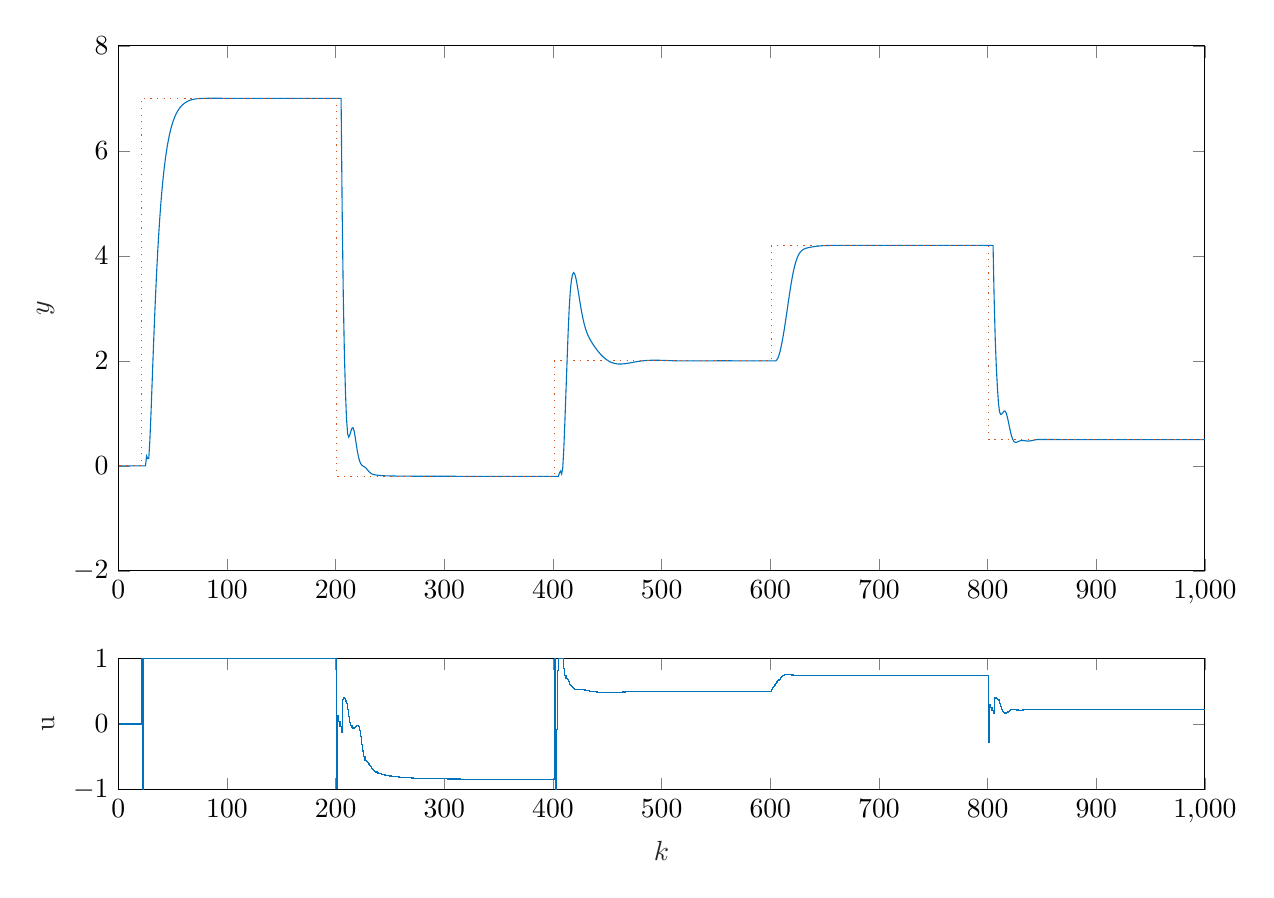
\begin{tikzpicture}

\begin{axis}[%
width=5.433in,
height=0.656in,
at={(0.854in,0.525in)},
scale only axis,
xmin=0,
xmax=1000,
xtick={0,100,200,300,400,500,600,700,800,900,1000},
xlabel style={font=\color{white!15!black}},
xlabel={$k$},
ymin=-1,
ymax=1,
ytick={-1,0,1},
ylabel style={font=\color{white!15!black}},
ylabel={u},
axis background/.style={fill=white}
]
\addplot[const plot, color=mycolor1, forget plot] table[row sep=crcr] {%
1	0\\
2	0\\
3	0\\
4	0\\
5	0\\
6	0\\
7	0\\
8	0\\
9	0\\
10	0\\
11	0\\
12	0\\
13	0\\
14	0\\
15	0\\
16	0\\
17	0\\
18	0\\
19	0\\
20	0\\
21	1\\
22	-1\\
23	1\\
24	1\\
25	1\\
26	1\\
27	1\\
28	1\\
29	1\\
30	1\\
31	1\\
32	1\\
33	1\\
34	1\\
35	1\\
36	1\\
37	1\\
38	1\\
39	1\\
40	1\\
41	1\\
42	1\\
43	1\\
44	1\\
45	1\\
46	1\\
47	1\\
48	1\\
49	1\\
50	1\\
51	1\\
52	1\\
53	1\\
54	1\\
55	1\\
56	1\\
57	0.999967792005714\\
58	0.999906795895747\\
59	0.999820555438343\\
60	0.999712178671646\\
61	0.999584391282136\\
62	0.999443255915826\\
63	0.999295235256106\\
64	0.999145755154132\\
65	0.998999427336996\\
66	0.99886022102646\\
67	0.99873116336803\\
68	0.99861422443403\\
69	0.998510479276465\\
70	0.998420275299083\\
71	0.998343349901601\\
72	0.998278965190922\\
73	0.998226060518648\\
74	0.998183384626228\\
75	0.998149598985531\\
76	0.998123361053089\\
77	0.998103389018131\\
78	0.998088506067676\\
79	0.998077666388698\\
80	0.998069967274796\\
81	0.998064650610117\\
82	0.998061096249721\\
83	0.998058809908799\\
84	0.998057407959561\\
85	0.998056600937481\\
86	0.998056177051968\\
87	0.998055986650705\\
88	0.998055928266632\\
89	0.998055936576084\\
90	0.998055972370206\\
91	0.99805601448927\\
92	0.998056053565099\\
93	0.998056087350562\\
94	0.998056117384697\\
95	0.998056146739094\\
96	0.998056178605744\\
97	0.99805621551174\\
98	0.998056258977744\\
99	0.998056309470734\\
100	0.998056366534156\\
101	0.998056429008229\\
102	0.998056495278829\\
103	0.998056563514537\\
104	0.99805663186818\\
105	0.998056698631723\\
106	0.998056762342214\\
107	0.998056821842335\\
108	0.99805687630244\\
109	0.998056925212531\\
110	0.998056968352791\\
111	0.998057005750648\\
112	0.998057037631186\\
113	0.998057064366288\\
114	0.998057086426513\\
115	0.998057104338338\\
116	0.998057118648279\\
117	0.998057129894479\\
118	0.998057138585644\\
119	0.998057145186737\\
120	0.998057150110521\\
121	0.998057153713927\\
122	0.998057156298162\\
123	0.998057158111547\\
124	0.99805715935417\\
125	0.998057160183601\\
126	0.998057160721043\\
127	0.998057161057456\\
128	0.99805716125933\\
129	0.998057161373884\\
130	0.998057161433582\\
131	0.998057161459933\\
132	0.998057161466573\\
133	0.998057161461697\\
134	0.998057161449913\\
135	0.998057161433603\\
136	0.998057161413883\\
137	0.998057161391242\\
138	0.998057161365943\\
139	0.998057161338247\\
140	0.998057161308516\\
141	0.998057161277233\\
142	0.998057161244983\\
143	0.998057161212409\\
144	0.99805716118016\\
145	0.998057161148847\\
146	0.998057161119006\\
147	0.998057161091072\\
148	0.998057161065367\\
149	0.998057161042101\\
150	0.998057161021373\\
151	0.998057161003188\\
152	0.99805716098747\\
153	0.998057160974081\\
154	0.99805716096284\\
155	0.998057160953533\\
156	0.998057160945936\\
157	0.998057160939821\\
158	0.998057160934969\\
159	0.998057160931174\\
160	0.998057160928248\\
161	0.998057160926025\\
162	0.998057160924363\\
163	0.998057160923139\\
164	0.998057160922252\\
165	0.998057160921621\\
166	0.998057160921179\\
167	0.998057160920877\\
168	0.998057160920675\\
169	0.998057160920542\\
170	0.998057160920458\\
171	0.998057160920407\\
172	0.99805716092038\\
173	0.998057160920366\\
174	0.998057160920363\\
175	0.998057160920366\\
176	0.998057160920374\\
177	0.998057160920384\\
178	0.998057160920396\\
179	0.99805716092041\\
180	0.998057160920425\\
181	0.99805716092044\\
182	0.998057160920455\\
183	0.998057160920471\\
184	0.998057160920487\\
185	0.998057160920502\\
186	0.998057160920516\\
187	0.99805716092053\\
188	0.998057160920542\\
189	0.998057160920553\\
190	0.998057160920562\\
191	0.998057160920571\\
192	0.998057160920579\\
193	0.998057160920585\\
194	0.998057160920591\\
195	0.998057160920596\\
196	0.9980571609206\\
197	0.998057160920604\\
198	0.998057160920607\\
199	0.998057160920609\\
200	0.998057160920611\\
201	-0.98557212865215\\
202	0.126816096562765\\
203	0.0429373642271256\\
204	-0.0409413681085142\\
205	-0.124820100444154\\
206	0.379955620881731\\
207	0.408036936431627\\
208	0.391419281898815\\
209	0.350864523868361\\
210	0.310100748390507\\
211	0.226131908316316\\
212	0.1102509620996\\
213	0.0273144140697846\\
214	-0.0238597653980417\\
215	-0.057306252276285\\
216	-0.0685197337725652\\
217	-0.0542501125008032\\
218	-0.0339947167814659\\
219	-0.0227939058090223\\
220	-0.0236774706138384\\
221	-0.0333480913661423\\
222	-0.0952271954121185\\
223	-0.194751563732025\\
224	-0.306607980202009\\
225	-0.410973483445239\\
226	-0.497107491390252\\
227	-0.552019378384978\\
228	-0.57509480133661\\
229	-0.589963728622156\\
230	-0.609127496879482\\
231	-0.631091207729951\\
232	-0.652053093459274\\
233	-0.671674415716614\\
234	-0.690919687352486\\
235	-0.707922203691887\\
236	-0.721350050213989\\
237	-0.731745835727178\\
238	-0.740234556294718\\
239	-0.747419434023677\\
240	-0.753456778646587\\
241	-0.758730719108263\\
242	-0.763592388447376\\
243	-0.768141646078001\\
244	-0.772346774100528\\
245	-0.776206428636372\\
246	-0.779774212731911\\
247	-0.783075487086272\\
248	-0.786120541712304\\
249	-0.788935803634669\\
250	-0.791558354252119\\
251	-0.794017561759486\\
252	-0.796330015585993\\
253	-0.798510041751863\\
254	-0.800571284539877\\
255	-0.802523809420263\\
256	-0.804374421565133\\
257	-0.806129058663647\\
258	-0.807794010698087\\
259	-0.809375034082102\\
260	-0.810877103099984\\
261	-0.812304824394811\\
262	-0.813662596960855\\
263	-0.814954461084008\\
264	-0.81618400165794\\
265	-0.817354491006543\\
266	-0.818468989415725\\
267	-0.819530348264188\\
268	-0.820541216090125\\
269	-0.821504076577217\\
270	-0.82242128344204\\
271	-0.823295064748438\\
272	-0.824127524455802\\
273	-0.824920653219907\\
274	-0.82567633923148\\
275	-0.826396374089936\\
276	-0.827082456955214\\
277	-0.827736200950125\\
278	-0.828359139548057\\
279	-0.828952731282097\\
280	-0.829518363648979\\
281	-0.830057357044489\\
282	-0.8305709685832\\
283	-0.831060395366719\\
284	-0.831526777412188\\
285	-0.831971200498747\\
286	-0.832394698902172\\
287	-0.832798257935319\\
288	-0.833182816312878\\
289	-0.833549268408665\\
290	-0.833898466407033\\
291	-0.834231222330339\\
292	-0.834548309951888\\
293	-0.834850466613514\\
294	-0.835138394955974\\
295	-0.835412764561806\\
296	-0.835674213515571\\
297	-0.835923349889102\\
298	-0.836160753156324\\
299	-0.836386975540185\\
300	-0.836602543294789\\
301	-0.836807957926656\\
302	-0.837003697358325\\
303	-0.837190217036883\\
304	-0.837367950990019\\
305	-0.837537312832312\\
306	-0.837698696724199\\
307	-0.83785247828587\\
308	-0.837999015468198\\
309	-0.838138649382779\\
310	-0.838271705093022\\
311	-0.838398492368139\\
312	-0.838519306401745\\
313	-0.838634428496758\\
314	-0.838744126718174\\
315	-0.838848656515227\\
316	-0.838948261314362\\
317	-0.839043173084394\\
318	-0.839133612875155\\
319	-0.839219791330867\\
320	-0.839301909179427\\
321	-0.839380157698731\\
322	-0.839454719161105\\
323	-0.839525767256883\\
324	-0.839593467498088\\
325	-0.839657977603164\\
326	-0.839719447863637\\
327	-0.839778021493555\\
328	-0.839833834962508\\
329	-0.839887018313011\\
330	-0.839937695462967\\
331	-0.839985984493909\\
332	-0.840031997925712\\
333	-0.840075842978374\\
334	-0.840117621821499\\
335	-0.840157431812048\\
336	-0.840195365720911\\
337	-0.840231511948821\\
338	-0.840265954732116\\
339	-0.840298774338819\\
340	-0.840330047255501\\
341	-0.840359846365345\\
342	-0.840388241117834\\
343	-0.840415297690462\\
344	-0.840441079142821\\
345	-0.840465645563453\\
346	-0.840489054209778\\
347	-0.84051135964144\\
348	-0.840532613847381\\
349	-0.840552866366926\\
350	-0.840572164405171\\
351	-0.840590552942941\\
352	-0.840608074841567\\
353	-0.840624770942731\\
354	-0.840640680163613\\
355	-0.840655839587554\\
356	-0.840670284550449\\
357	-0.840684048723076\\
358	-0.840697164189545\\
359	-0.840709661522049\\
360	-0.840721569852105\\
361	-0.840732916938425\\
362	-0.840743729231605\\
363	-0.840754031935754\\
364	-0.84076384906723\\
365	-0.840773203510606\\
366	-0.840782117071994\\
367	-0.840790610529867\\
368	-0.840798703683481\\
369	-0.840806415399015\\
370	-0.84081376365354\\
371	-0.840820765576916\\
372	-0.840827437491716\\
373	-0.840833794951266\\
374	-0.840839852775893\\
375	-0.840845625087472\\
376	-0.840851125342335\\
377	-0.840856366362637\\
378	-0.840861360366242\\
379	-0.840866118995198\\
380	-0.840870653342875\\
381	-0.840874973979822\\
382	-0.840879090978404\\
383	-0.84088301393628\\
384	-0.840886751998778\\
385	-0.840890313880205\\
386	-0.840893707884166\\
387	-0.840896941922919\\
388	-0.840900023535813\\
389	-0.840902959906868\\
390	-0.840905757881521\\
391	-0.840908423982578\\
392	-0.840910964425423\\
393	-0.840913385132507\\
394	-0.84091569174715\\
395	-0.840917889646699\\
396	-0.840919983955065\\
397	-0.84092197955466\\
398	-0.840923881097788\\
399	-0.840925693017484\\
400	-0.840927419537847\\
401	1\\
402	-1\\
403	-0.0901981180311768\\
404	0.8196038343398\\
405	1\\
406	1\\
407	1\\
408	1\\
409	1\\
410	0.851605616326322\\
411	0.7398392607538\\
412	0.688128100410775\\
413	0.68431135834817\\
414	0.646466361529332\\
415	0.604790426243364\\
416	0.580618223258783\\
417	0.565261897153952\\
418	0.550247005346982\\
419	0.538506457374307\\
420	0.532196093406113\\
421	0.52894514443087\\
422	0.526885716635701\\
423	0.525854922197161\\
424	0.525559961295753\\
425	0.525289581557752\\
426	0.524648367300166\\
427	0.523475454761727\\
428	0.521226525496063\\
429	0.518278501367673\\
430	0.514949359856683\\
431	0.511481366928381\\
432	0.508037665412243\\
433	0.504750719998199\\
434	0.501689788654275\\
435	0.498876763692924\\
436	0.496310442639313\\
437	0.493980308841454\\
438	0.491872509615065\\
439	0.489973813833706\\
440	0.488273434747633\\
441	0.486762948688988\\
442	0.485435495247878\\
443	0.484284967716401\\
444	0.48330539277012\\
445	0.482490534727124\\
446	0.48183369550215\\
447	0.481342816798865\\
448	0.481021139532331\\
449	0.480853540243322\\
450	0.480825195599306\\
451	0.480921643959485\\
452	0.481128725635595\\
453	0.481432514065363\\
454	0.481819389727519\\
455	0.482276154843043\\
456	0.482790141290509\\
457	0.483349305520104\\
458	0.483942307751986\\
459	0.484558574888159\\
460	0.485188347464102\\
461	0.485822711559008\\
462	0.486453616893021\\
463	0.48707388246933\\
464	0.487677191150036\\
465	0.488258074531193\\
466	0.488811889428865\\
467	0.489334787218159\\
468	0.489823677189308\\
469	0.490276185003878\\
470	0.490690607253086\\
471	0.491065863040737\\
472	0.491401443436471\\
473	0.491697359571229\\
474	0.491954090076219\\
475	0.492172528499217\\
476	0.492353931267439\\
477	0.49249986670436\\
478	0.492612165548495\\
479	0.492692873365039\\
480	0.49274420518635\\
481	0.492768502664392\\
482	0.492768193967453\\
483	0.492745756604763\\
484	0.4927036833161\\
485	0.4926444511193\\
486	0.492570493566832\\
487	0.492484176223559\\
488	0.492387775341524\\
489	0.492283459674382\\
490	0.492173275343988\\
491	0.49205913364485\\
492	0.491942801648726\\
493	0.491825895451647\\
494	0.49170987588909\\
495	0.491596046531899\\
496	0.491485553765748\\
497	0.491379388750371\\
498	0.491278391051282\\
499	0.491183253736057\\
500	0.491094529729272\\
501	0.491012639224611\\
502	0.490937877959209\\
503	0.490870426163696\\
504	0.490810358011432\\
505	0.490757651401667\\
506	0.490712197923708\\
507	0.490673812862197\\
508	0.490642245117164\\
509	0.490617186926348\\
510	0.490598283291097\\
511	0.490585141020909\\
512	0.490577337325025\\
513	0.490574427892434\\
514	0.490575954413935\\
515	0.490581451511591\\
516	0.490590453051689\\
517	0.490602497827414\\
518	0.490617134606528\\
519	0.490633926547633\\
520	0.490652454995903\\
521	0.490672322675609\\
522	0.490693156302313\\
523	0.490714608642288\\
524	0.490736360050551\\
525	0.490758119522019\\
526	0.490779625292579\\
527	0.490800645028546\\
528	0.490820975643984\\
529	0.490840442785792\\
530	0.490858900026378\\
531	0.490876227803198\\
532	0.490892332143437\\
533	0.490907143210833\\
534	0.490920613709984\\
535	0.490932717181609\\
536	0.49094344622015\\
537	0.490952810642862\\
538	0.490960835637152\\
539	0.490967559910526\\
540	0.490973033864968\\
541	0.490977317815145\\
542	0.490980480267303\\
543	0.490982596273341\\
544	0.49098374587217\\
545	0.490984012628236\\
546	0.490983482274896\\
547	0.490982241468355\\
548	0.490980376655949\\
549	0.490977973060824\\
550	0.490975113783466\\
551	0.490971879019096\\
552	0.490968345388648\\
553	0.490964585379924\\
554	0.490960666894556\\
555	0.490956652895546\\
556	0.490952601149506\\
557	0.49094856405716\\
558	0.490944588565261\\
559	0.490940716152788\\
560	0.490936982884116\\
561	0.490933419521782\\
562	0.490930051691496\\
563	0.490926900092154\\
564	0.490923980743808\\
565	0.490921305266801\\
566	0.490918881185561\\
567	0.490916712250946\\
568	0.490914798775391\\
569	0.490913137975543\\
570	0.490911724317532\\
571	0.49091054986045\\
572	0.49090960459411\\
573	0.490908876767604\\
574	0.490908353205636\\
575	0.490908019610081\\
576	0.490907860844627\\
577	0.49090786120079\\
578	0.490908004643998\\
579	0.490908275038781\\
580	0.490908656352494\\
581	0.490909132837268\\
582	0.490909689190217\\
583	0.490910310692165\\
584	0.490910983325389\\
585	0.490911693871091\\
586	0.490912429987456\\
587	0.490913180269337\\
588	0.490913934290681\\
589	0.490914682630945\\
590	0.490915416886783\\
591	0.490916129670359\\
592	0.490916814595652\\
593	0.490917466254117\\
594	0.490918080181084\\
595	0.490918652814214\\
596	0.490919181445326\\
597	0.49091966416682\\
598	0.490920099813915\\
599	0.490920487903774\\
600	0.490920828572607\\
601	0.528625922818229\\
602	0.550118048237556\\
603	0.572783534704553\\
604	0.595448979207339\\
605	0.618114384024528\\
606	0.640512014672628\\
607	0.66240489154129\\
608	0.68332691445079\\
609	0.702658075694036\\
610	0.719853769597616\\
611	0.734395442993946\\
612	0.745816310898272\\
613	0.753741401548071\\
614	0.757946371188769\\
615	0.758622875048564\\
616	0.757851641028586\\
617	0.755976304574615\\
618	0.753390733690733\\
619	0.75052366797075\\
620	0.747792006870868\\
621	0.745379939186376\\
622	0.74336936764076\\
623	0.741808161226642\\
624	0.74069865770401\\
625	0.739994628634819\\
626	0.739627267600708\\
627	0.739523868510288\\
628	0.739612520769973\\
629	0.739826070920012\\
630	0.740107429314587\\
631	0.7404120803427\\
632	0.740707646687337\\
633	0.740972651032053\\
634	0.741195072665155\\
635	0.741370469737733\\
636	0.741499896554562\\
637	0.741588020238708\\
638	0.74164156561255\\
639	0.741668068012792\\
640	0.741674939407564\\
641	0.741668849810575\\
642	0.74165537976273\\
643	0.741638880636118\\
644	0.741622487705747\\
645	0.741608238102177\\
646	0.741597249483049\\
647	0.741589923007773\\
648	0.741586144580403\\
649	0.74158546718853\\
650	0.7415872640621\\
651	0.741590848177026\\
652	0.741595558201401\\
653	0.741600814006767\\
654	0.741606146562116\\
655	0.741611207774929\\
656	0.741615765876976\\
657	0.74161969145983\\
658	0.741622938460448\\
659	0.741625523466904\\
660	0.741627505782147\\
661	0.741628969829486\\
662	0.741630010759817\\
663	0.741630723552605\\
664	0.741631195491383\\
665	0.741631501626141\\
666	0.741631702687902\\
667	0.741631844869453\\
668	0.741631960904505\\
669	0.74163207194132\\
670	0.741632189795748\\
671	0.741632319266588\\
672	0.741632460291397\\
673	0.741632609805679\\
674	0.7416327632384\\
675	0.741632915630424\\
676	0.74163306240024\\
677	0.741633199804799\\
678	0.741633325154985\\
679	0.741633436847853\\
680	0.741633534274021\\
681	0.741633617650769\\
682	0.741633687821624\\
683	0.741633746052888\\
684	0.741633793847858\\
685	0.741633832791042\\
686	0.741633864427862\\
687	0.741633890180232\\
688	0.741633911294915\\
689	0.741633928819497\\
690	0.741633943599897\\
691	0.741633956293245\\
692	0.741633967390508\\
693	0.741633977244094\\
694	0.741633986096699\\
695	0.7416339941087\\
696	0.741634001382364\\
697	0.741634007981947\\
698	0.74163401394938\\
699	0.741634019315743\\
700	0.741634024108981\\
701	0.741634028358515\\
702	0.741634032097451\\
703	0.741634035363051\\
704	0.741634038196085\\
705	0.741634040639545\\
706	0.741634042737115\\
707	0.741634044531684\\
708	0.74163404606405\\
709	0.741634047371936\\
710	0.741634048489338\\
711	0.741634049446187\\
712	0.741634050268289\\
713	0.74163405097749\\
714	0.741634051591982\\
715	0.741634052126723\\
716	0.741634052593892\\
717	0.741634053003351\\
718	0.741634053363082\\
719	0.741634053679576\\
720	0.741634053958171\\
721	0.741634054203321\\
722	0.741634054418816\\
723	0.741634054607942\\
724	0.741634054773601\\
725	0.741634054918395\\
726	0.741634055044676\\
727	0.741634055154586\\
728	0.741634055250074\\
729	0.741634055332908\\
730	0.74163405540469\\
731	0.741634055466852\\
732	0.741634055520674\\
733	0.741634055567283\\
734	0.741634055607672\\
735	0.741634055642698\\
736	0.741634055673107\\
737	0.741634055699538\\
738	0.741634055722538\\
739	0.741634055742575\\
740	0.741634055760046\\
741	0.741634055775292\\
742	0.741634055788602\\
743	0.741634055800224\\
744	0.741634055810374\\
745	0.741634055819236\\
746	0.741634055826969\\
747	0.741634055833715\\
748	0.741634055839597\\
749	0.741634055844721\\
750	0.741634055849183\\
751	0.741634055853066\\
752	0.741634055856444\\
753	0.741634055859382\\
754	0.741634055861936\\
755	0.741634055864156\\
756	0.741634055866087\\
757	0.741634055867765\\
758	0.741634055869225\\
759	0.741634055870494\\
760	0.741634055871599\\
761	0.741634055872561\\
762	0.741634055873398\\
763	0.741634055874128\\
764	0.741634055874763\\
765	0.741634055875316\\
766	0.741634055875798\\
767	0.741634055876219\\
768	0.741634055876585\\
769	0.741634055876904\\
770	0.741634055877182\\
771	0.741634055877424\\
772	0.741634055877636\\
773	0.741634055877819\\
774	0.741634055877979\\
775	0.741634055878118\\
776	0.741634055878239\\
777	0.741634055878344\\
778	0.741634055878437\\
779	0.741634055878516\\
780	0.741634055878586\\
781	0.741634055878646\\
782	0.741634055878699\\
783	0.741634055878745\\
784	0.741634055878785\\
785	0.74163405587882\\
786	0.74163405587885\\
787	0.741634055878876\\
788	0.741634055878899\\
789	0.74163405587892\\
790	0.741634055878937\\
791	0.741634055878952\\
792	0.741634055878965\\
793	0.741634055878977\\
794	0.741634055878987\\
795	0.741634055878995\\
796	0.741634055879003\\
797	0.74163405587901\\
798	0.741634055879016\\
799	0.741634055879021\\
800	0.741634055879025\\
801	-0.277730995706974\\
802	0.293912953361805\\
803	0.250808604800437\\
804	0.207704256239069\\
805	0.1645999076777\\
806	0.400157868139949\\
807	0.397237719927082\\
808	0.386180217460633\\
809	0.371225694052644\\
810	0.36617385316509\\
811	0.31542799635836\\
812	0.261055078562572\\
813	0.222536471430091\\
814	0.195196069119405\\
815	0.17308723221437\\
816	0.16443965568716\\
817	0.170361692458966\\
818	0.182857624970205\\
819	0.196205734022884\\
820	0.208704190697366\\
821	0.218221709888399\\
822	0.223939547908677\\
823	0.225674573107945\\
824	0.224514925806654\\
825	0.221546769905761\\
826	0.217825318813683\\
827	0.214323511888519\\
828	0.211821697705766\\
829	0.210688357601227\\
830	0.210928984660478\\
831	0.212318371256434\\
832	0.214486138151053\\
833	0.216991147695336\\
834	0.219422836350882\\
835	0.221475159051106\\
836	0.222967930946062\\
837	0.223841828863233\\
838	0.224143333873131\\
839	0.223995426983805\\
840	0.223558521480947\\
841	0.222994946487919\\
842	0.222443191596031\\
843	0.222001510864279\\
844	0.22172125782931\\
845	0.22161017214074\\
846	0.221642736001585\\
847	0.221773437165933\\
848	0.221949949182295\\
849	0.222124268947675\\
850	0.222260341939755\\
851	0.222337592976606\\
852	0.222350825855545\\
853	0.222307489937632\\
854	0.22222341263742\\
855	0.22211808061785\\
856	0.222010412849941\\
857	0.221915651908083\\
858	0.221843631091577\\
859	0.221798378495549\\
860	0.221778808728763\\
861	0.221780122176245\\
862	0.221795496464999\\
863	0.221817707961836\\
864	0.221840424585981\\
865	0.221859030103139\\
866	0.221870953734896\\
867	0.221875570778751\\
868	0.221873797578627\\
869	0.22186752562308\\
870	0.221859031185282\\
871	0.221850467722528\\
872	0.221843507736007\\
873	0.221839158594682\\
874	0.221837740873298\\
875	0.221838992682414\\
876	0.221842250782974\\
877	0.221846658142618\\
878	0.221851355433319\\
879	0.221855627215784\\
880	0.221858988561595\\
881	0.221861211624378\\
882	0.221862302141472\\
883	0.221862442030826\\
884	0.221861916128917\\
885	0.22186103943229\\
886	0.221860097124684\\
887	0.221859304480507\\
888	0.2218587885964\\
889	0.221858589687311\\
890	0.221858676890264\\
891	0.221858972278323\\
892	0.221859376931352\\
893	0.221859794074766\\
894	0.221860146031957\\
895	0.221860383602465\\
896	0.221860488123154\\
897	0.221860467665642\\
898	0.221860349474949\\
899	0.221860170883648\\
900	0.2218599706489\\
901	0.221859782108399\\
902	0.221859628895076\\
903	0.221859523328163\\
904	0.221859467108422\\
905	0.221859453639805\\
906	0.221859471185733\\
907	0.221859506118303\\
908	0.221859545683972\\
909	0.221859579933132\\
910	0.221859602690504\\
911	0.221859611637657\\
912	0.22185960771345\\
913	0.221859594104354\\
914	0.221859575099859\\
915	0.221859555043436\\
916	0.221859537536188\\
917	0.221859524968106\\
918	0.221859518376958\\
919	0.221859517578406\\
920	0.221859521478109\\
921	0.221859528467144\\
922	0.221859536811954\\
923	0.221859544972794\\
924	0.22185955181311\\
925	0.22185955669032\\
926	0.221859559441157\\
927	0.221859560289695\\
928	0.221859559712559\\
929	0.221859558294751\\
930	0.221859556602953\\
931	0.221859555093606\\
932	0.221859554062858\\
933	0.22185955363657\\
934	0.221859553792155\\
935	0.221859554400606\\
936	0.221859555276451\\
937	0.221859556225073\\
938	0.22185955707987\\
939	0.221859557725343\\
940	0.221859558105599\\
941	0.221859558220366\\
942	0.221859558112301\\
943	0.221859557849886\\
944	0.221859557509968\\
945	0.221859557163033\\
946	0.221859556863075\\
947	0.221859556642707\\
948	0.221859556513055\\
949	0.22185955646731\\
950	0.221859556486425\\
951	0.221859556545472\\
952	0.221859556619413\\
953	0.221859556687434\\
954	0.221859556735475\\
955	0.221859556756953\\
956	0.221859556752019\\
957	0.221859556725824\\
958	0.221859556686357\\
959	0.221859556642317\\
960	0.221859556601392\\
961	0.221859556569133\\
962	0.221859556548478\\
963	0.221859556539846\\
964	0.22185955654164\\
965	0.221859556550989\\
966	0.221859556564517\\
967	0.221859556579028\\
968	0.221859556591983\\
969	0.221859556601765\\
970	0.221859556607711\\
971	0.221859556609981\\
972	0.221859556609322\\
973	0.221859556606791\\
974	0.221859556603487\\
975	0.221859556600354\\
976	0.221859556598057\\
977	0.22185955659693\\
978	0.221859556597004\\
979	0.22185955659808\\
980	0.221859556599813\\
981	0.221859556601817\\
982	0.221859556603737\\
983	0.221859556605309\\
984	0.221859556606382\\
985	0.221859556606917\\
986	0.22185955660697\\
987	0.221859556606661\\
988	0.221859556606135\\
989	0.221859556605537\\
990	0.221859556604984\\
991	0.221859556604555\\
992	0.221859556604288\\
993	0.221859556604181\\
994	0.221859556604205\\
995	0.221859556604317\\
996	0.221859556604467\\
997	0.221859556604614\\
998	0.221859556604726\\
999	0.221859556604786\\
1000	0.221859556604792\\
};
\end{axis}

\begin{axis}[%
width=5.433in,
height=2.625in,
at={(0.854in,1.619in)},
scale only axis,
xmin=0,
xmax=1000,
xtick={0,100,200,300,400,500,600,700,800,900,1000},
ymin=-2,
ymax=8,
ytick={-2,0,2,4,6,8},
ylabel style={font=\color{white!15!black}},
ylabel={$y$},
axis background/.style={fill=white}
]
\addplot [color=mycolor1, forget plot]
  table[row sep=crcr]{%
1	0\\
2	0\\
3	0\\
4	0\\
5	0\\
6	0\\
7	0\\
8	0\\
9	0\\
10	0\\
11	0\\
12	0\\
13	0\\
14	0\\
15	0\\
16	0\\
17	0\\
18	0\\
19	0\\
20	0\\
21	0\\
22	0\\
23	0\\
24	0\\
25	0\\
26	0.187021166666667\\
27	0.1388412867175\\
28	0.140250690946808\\
29	0.474484324849734\\
30	0.969546331063805\\
31	1.52616259558225\\
32	2.0885485281946\\
33	2.626753768434\\
34	3.12601990380585\\
35	3.58038393470303\\
36	3.98884990759164\\
37	4.35311200695019\\
38	4.67621316346153\\
39	4.9617662410529\\
40	5.21351218539529\\
41	5.43507880520345\\
42	5.62985795429437\\
43	5.80095163977713\\
44	5.95115740202629\\
45	6.08297529098591\\
46	6.19862599114077\\
47	6.30007399804402\\
48	6.38905235869494\\
49	6.46708704494637\\
50	6.53551995075424\\
51	6.59553004318073\\
52	6.64815250657622\\
53	6.69429589177026\\
54	6.73475737322811\\
55	6.77023626060868\\
56	6.80134592719055\\
57	6.82862431828721\\
58	6.85254319521671\\
59	6.87351625883499\\
60	6.89190628351707\\
61	6.90803137914879\\
62	6.9221571561818\\
63	6.9345048807561\\
64	6.94526348334981\\
65	6.95459735979641\\
66	6.96265149037602\\
67	6.96955643533663\\
68	6.97543237470589\\
69	6.98039139530736\\
70	6.98453860470391\\
71	6.9879726710904\\
72	6.99078593221572\\
73	6.99306417508938\\
74	6.9948863004818\\
75	6.99632403668614\\
76	6.99744176799967\\
77	6.99829650681382\\
78	6.99893802783778\\
79	6.99940916071317\\
80	6.99974621621313\\
81	6.99997951353735\\
82	7.00013397569175\\
83	7.00022976068341\\
84	7.00028289884826\\
85	7.00030591161241\\
86	7.00030839287583\\
87	7.00029753980915\\
88	7.00027862495347\\
89	7.00025540602186\\
90	7.00023047349442\\
91	7.00020553887543\\
92	7.00018166841368\\
93	7.00015946828966\\
94	7.00013922785523\\
95	7.00012102759434\\
96	7.0001048181887\\
97	7.00009047653904\\
98	7.00007784390936\\
99	7.00006675060903\\
100	7.00005703086864\\
101	7.00004853084565\\
102	7.00004111204475\\
103	7.00003465187109\\
104	7.00002904256012\\
105	7.00002418934281\\
106	7.00002000840512\\
107	7.0000164249744\\
108	7.00001337170301\\
109	7.00001078740873\\
110	7.00000861616136\\
111	7.00000680666561\\
112	7.00000531187304\\
113	7.00000408875293\\
114	7.00000309815896\\
115	7.00000230473974\\
116	7.00000167685456\\
117	7.0000011864689\\
118	7.00000080901528\\
119	7.00000052321473\\
120	7.00000031086074\\
121	7.00000015657224\\
122	7.00000004752475\\
123	6.99999997316982\\
124	6.99999992495278\\
125	6.99999989603735\\
126	6.99999988104468\\
127	6.99999987581205\\
128	6.99999987717502\\
129	6.9999998827749\\
130	6.99999989089225\\
131	6.99999990030561\\
132	6.99999991017405\\
133	6.99999991994143\\
134	6.99999992925994\\
135	6.99999993793013\\
136	6.99999994585509\\
137	6.99999995300612\\
138	6.99999995939768\\
139	6.99999996506965\\
140	6.9999999700752\\
141	6.99999997447284\\
142	6.99999997832141\\
143	6.99999998167729\\
144	6.99999998459295\\
145	6.99999998711645\\
146	6.9999999892914\\
147	6.99999999115726\\
148	6.99999999274972\\
149	6.99999999410112\\
150	6.99999999524078\\
151	6.99999999619533\\
152	6.99999999698892\\
153	6.99999999764344\\
154	6.99999999817861\\
155	6.99999999861215\\
156	6.99999999895987\\
157	6.99999999923574\\
158	6.99999999945204\\
159	6.99999999961943\\
160	6.99999999974709\\
161	6.99999999984284\\
162	6.99999999991327\\
163	6.99999999996385\\
164	6.9999999999991\\
165	7.00000000002269\\
166	7.00000000003756\\
167	7.00000000004603\\
168	7.00000000004993\\
169	7.00000000005065\\
170	7.00000000004925\\
171	7.00000000004651\\
172	7.00000000004299\\
173	7.00000000003909\\
174	7.00000000003511\\
175	7.00000000003121\\
176	7.00000000002751\\
177	7.00000000002407\\
178	7.00000000002094\\
179	7.00000000001812\\
180	7.00000000001559\\
181	7.00000000001336\\
182	7.00000000001139\\
183	7.00000000000966\\
184	7.00000000000815\\
185	7.00000000000685\\
186	7.00000000000572\\
187	7.00000000000474\\
188	7.00000000000391\\
189	7.00000000000321\\
190	7.00000000000261\\
191	7.00000000000211\\
192	7.00000000000169\\
193	7.00000000000134\\
194	7.00000000000105\\
195	7.00000000000082\\
196	7.00000000000062\\
197	7.00000000000047\\
198	7.00000000000034\\
199	7.00000000000025\\
200	7.00000000000017\\
201	7.00000000000011\\
202	7.00000000000007\\
203	7.00000000000004\\
204	7.00000000000002\\
205	7\\
206	4.86335476661778\\
207	3.25877503965814\\
208	2.17426882188505\\
209	1.42137030951934\\
210	0.895123794698472\\
211	0.614020737914612\\
212	0.546688791774948\\
213	0.585635292728324\\
214	0.656169417152532\\
215	0.71534122313945\\
216	0.727189155386562\\
217	0.664393041072631\\
218	0.544373426924386\\
219	0.405623026686709\\
220	0.276698766045633\\
221	0.171708684055633\\
222	0.0948990308409751\\
223	0.0444452939472361\\
224	0.0145071166139491\\
225	-0.0024237052148406\\
226	-0.0130117716659548\\
227	-0.0253970817363073\\
228	-0.0451277639166907\\
229	-0.0699023273883214\\
230	-0.0948053392893026\\
231	-0.116798648429278\\
232	-0.134945932435311\\
233	-0.149047138717289\\
234	-0.159127388388847\\
235	-0.166011667680915\\
236	-0.170872568499127\\
237	-0.174580885193654\\
238	-0.177584916270307\\
239	-0.180120444884648\\
240	-0.182357600646744\\
241	-0.184353286192231\\
242	-0.186088985545675\\
243	-0.187553763727732\\
244	-0.188773027993882\\
245	-0.189787731723148\\
246	-0.190633029572913\\
247	-0.19134323918988\\
248	-0.191952305795519\\
249	-0.192487013597412\\
250	-0.192964266664975\\
251	-0.193394364442267\\
252	-0.193785030560858\\
253	-0.194142010679587\\
254	-0.194469307354864\\
255	-0.194770168974126\\
256	-0.195047765868016\\
257	-0.195305113360156\\
258	-0.19554475455313\\
259	-0.195768790400265\\
260	-0.195978999043478\\
261	-0.19617685327775\\
262	-0.196363524801517\\
263	-0.19653995019753\\
264	-0.196706920523078\\
265	-0.196865123785212\\
266	-0.197015160790732\\
267	-0.197157563543288\\
268	-0.197292812972697\\
269	-0.197421347223671\\
270	-0.197543563400412\\
271	-0.197659821658879\\
272	-0.197770451153466\\
273	-0.197875754573974\\
274	-0.197976011278618\\
275	-0.198071480304737\\
276	-0.19816240340483\\
277	-0.19824900729757\\
278	-0.198331505171186\\
279	-0.198410097916466\\
280	-0.198484975242039\\
281	-0.198556316596257\\
282	-0.198624291895774\\
283	-0.198689062178921\\
284	-0.198750780223482\\
285	-0.198809591100364\\
286	-0.19886563265655\\
287	-0.198919035948319\\
288	-0.198969925639594\\
289	-0.199018420363297\\
290	-0.199064633047381\\
291	-0.199108671214163\\
292	-0.199150637259256\\
293	-0.19919062871193\\
294	-0.199228738478072\\
295	-0.19926505506826\\
296	-0.199299662812952\\
297	-0.19933264206565\\
298	-0.19936406939471\\
299	-0.199394017764754\\
300	-0.199422556708627\\
301	-0.199449752490513\\
302	-0.199475668260778\\
303	-0.199500364203061\\
304	-0.19952389767417\\
305	-0.199546323337181\\
306	-0.199567693288112\\
307	-0.199588057176534\\
308	-0.199607462320429\\
309	-0.199625953815601\\
310	-0.199643574639921\\
311	-0.199660365752639\\
312	-0.199676366189035\\
313	-0.199691613150614\\
314	-0.199706142091077\\
315	-0.19971998679826\\
316	-0.199733179472233\\
317	-0.199745750799752\\
318	-0.199757730025218\\
319	-0.199769145018327\\
320	-0.199780022338549\\
321	-0.199790387296597\\
322	-0.199800264013017\\
323	-0.19980967547404\\
324	-0.199818643584825\\
325	-0.199827189220202\\
326	-0.199835332273049\\
327	-0.199843091700402\\
328	-0.199850485567406\\
329	-0.199857531089209\\
330	-0.199864244670892\\
331	-0.199870641945533\\
332	-0.199876737810481\\
333	-0.199882546461936\\
334	-0.199888081427904\\
335	-0.199893355599611\\
336	-0.199898381261437\\
337	-0.199903170119452\\
338	-0.199907733328612\\
339	-0.199912081518678\\
340	-0.199916224818914\\
341	-0.199920172881636\\
342	-0.199923934904646\\
343	-0.199927519652615\\
344	-0.199930935477465\\
345	-0.199934190337789\\
346	-0.199937291817362\\
347	-0.199940247142776\\
348	-0.19994306320026\\
349	-0.199945746551692\\
350	-0.19994830344987\\
351	-0.19995073985306\\
352	-0.199953061438867\\
353	-0.199955273617441\\
354	-0.199957381544073\\
355	-0.199959390131196\\
356	-0.199961304059817\\
357	-0.199963127790419\\
358	-0.199964865573341\\
359	-0.199966521458677\\
360	-0.199968099305705\\
361	-0.199969602791876\\
362	-0.199971035421375\\
363	-0.199972400533283\\
364	-0.199973701309353\\
365	-0.199974940781422\\
366	-0.199976121838472\\
367	-0.199977247233357\\
368	-0.199978319589219\\
369	-0.199979341405596\\
370	-0.199980315064247\\
371	-0.199981242834698\\
372	-0.19998212687953\\
373	-0.199982969259419\\
374	-0.199983771937938\\
375	-0.199984536786126\\
376	-0.199985265586854\\
377	-0.199985960038977\\
378	-0.199986621761293\\
379	-0.199987252296312\\
380	-0.199987853113854\\
381	-0.199988425614474\\
382	-0.199988971132723\\
383	-0.199989490940261\\
384	-0.199989986248819\\
385	-0.199990458213023\\
386	-0.199990907933084\\
387	-0.199991336457364\\
388	-0.199991744784819\\
389	-0.199992133867326\\
390	-0.199992504611901\\
391	-0.199992857882815\\
392	-0.199993194503608\\
393	-0.199993515259006\\
394	-0.199993820896754\\
395	-0.199994112129356\\
396	-0.199994389635735\\
397	-0.199994654062818\\
398	-0.199994906027044\\
399	-0.199995146115797\\
400	-0.19999537488878\\
401	-0.199995592879316\\
402	-0.199995800595594\\
403	-0.19999599852185\\
404	-0.199996187119501\\
405	-0.199996366828215\\
406	-0.132164033326986\\
407	-0.100138608966333\\
408	-0.155075691267635\\
409	-0.0384600593722117\\
410	0.33806155073478\\
411	0.862225894360679\\
412	1.43952119149868\\
413	2.0171039872783\\
414	2.56685388658308\\
415	3.02569334457673\\
416	3.34677172839923\\
417	3.53919452936723\\
418	3.64465303154095\\
419	3.68132170542633\\
420	3.65524476148615\\
421	3.58132571479874\\
422	3.47735536589748\\
423	3.35592477926266\\
424	3.22642833911913\\
425	3.09745422380374\\
426	2.97559486215981\\
427	2.86465802994648\\
428	2.76641793862202\\
429	2.68132740138683\\
430	2.60877081979191\\
431	2.54736919739369\\
432	2.49534216175778\\
433	2.45057805123045\\
434	2.41105100338238\\
435	2.375121180301\\
436	2.34161206811054\\
437	2.30976860520007\\
438	2.27918047534992\\
439	2.24968596716622\\
440	2.22127584696788\\
441	2.19401752445355\\
442	2.16800453493291\\
443	2.14332695904008\\
444	2.12005702445748\\
445	2.09824465095552\\
446	2.07791845168403\\
447	2.059088981906\\
448	2.04175238176877\\
449	2.02589355424795\\
450	2.01148861600641\\
451	1.99850666313819\\
452	1.98691753201963\\
453	1.97669561172357\\
454	1.96781291313309\\
455	1.96023359024591\\
456	1.95391219599391\\
457	1.94879386135563\\
458	1.94481534363156\\
459	1.94190642190845\\
460	1.9399913957289\\
461	1.93899056372127\\
462	1.93882161872566\\
463	1.93940092840996\\
464	1.94064468820484\\
465	1.94246994323093\\
466	1.94479548132449\\
467	1.94754260224629\\
468	1.95063576974011\\
469	1.95400315387471\\
470	1.95757707139092\\
471	1.96129433177814\\
472	1.96509649664521\\
473	1.96893005970305\\
474	1.97274655438935\\
475	1.97650259586857\\
476	1.98015986385109\\
477	1.98368503240233\\
478	1.98704965265961\\
479	1.99022999414036\\
480	1.99320685010674\\
481	1.99596531224394\\
482	1.9984945197068\\
483	2.00078738738611\\
484	2.00284031803776\\
485	2.00465290269892\\
486	2.00622761358377\\
487	2.00756949340395\\
488	2.0086858447943\\
489	2.009585923244\\
490	2.01028063663604\\
491	2.0107822541879\\
492	2.01110412726495\\
493	2.01126042420911\\
494	2.01126588099285\\
495	2.01113556917678\\
496	2.01088468232145\\
497	2.01052834168587\\
498	2.01008142173943\\
499	2.00955839572511\\
500	2.00897320124226\\
501	2.00833912557019\\
502	2.00766871023147\\
503	2.00697367409706\\
504	2.00626485416562\\
505	2.00555216300745\\
506	2.00484456174756\\
507	2.00415004737404\\
508	2.00347565309388\\
509	2.00282746041888\\
510	2.00221062164629\\
511	2.00162939140137\\
512	2.00108716592924\\
513	2.00058652885917\\
514	2.00012930221428\\
515	1.99971660149998\\
516	1.99934889377434\\
517	1.99902605768058\\
518	1.99874744450368\\
519	1.99851193939852\\
520	1.99831802202427\\
521	1.99816382590715\\
522	1.99804719594053\\
523	1.99796574351597\\
524	1.99791689886101\\
525	1.99789796023763\\
526	1.99790613972963\\
527	1.99793860541689\\
528	1.99799251979881\\
529	1.99806507438878\\
530	1.99815352045544\\
531	1.99825519593526\\
532	1.99836754858378\\
533	1.99848815547129\\
534	1.99861473896083\\
535	1.99874517933445\\
536	1.99887752425645\\
537	1.99900999528047\\
538	1.99914099162162\\
539	1.9992690914245\\
540	1.99939305076462\\
541	1.99951180062326\\
542	1.99962444207597\\
543	1.99973023993163\\
544	1.99982861505368\\
545	1.9999191355876\\
546	2.000001507309\\
547	2.00007556329583\\
548	2.00014125311588\\
549	2.0001986317073\\
550	2.00024784811567\\
551	2.00028913423683\\
552	2.00032279369927\\
553	2.00034919100515\\
554	2.00036874103393\\
555	2.00038189899777\\
556	2.00038915092381\\
557	2.00039100472418\\
558	2.00038798190202\\
559	2.00038060992878\\
560	2.00036941531691\\
561	2.00035491740117\\
562	2.00033762283175\\
563	2.00031802077393\\
564	2.00029657880069\\
565	2.00027373945789\\
566	2.00024991747568\\
567	2.00022549759439\\
568	2.00020083296943\\
569	2.00017624411573\\
570	2.00015201835036\\
571	2.00012840968971\\
572	2.0001056391566\\
573	2.00008389545256\\
574	2.00006333595015\\
575	2.00004408796134\\
576	2.00002625023886\\
577	2.00000989466892\\
578	1.99999506811578\\
579	1.99998179438076\\
580	1.99997007624041\\
581	1.99995989753176\\
582	1.99995122525447\\
583	1.99994401166327\\
584	1.99993819632639\\
585	1.99993370812874\\
586	1.99993046720136\\
587	1.99992838676155\\
588	1.99992737485032\\
589	1.99992733595704\\
590	1.99992817252281\\
591	1.99992978631703\\
592	1.99993207968327\\
593	1.99993495665269\\
594	1.99993832392509\\
595	1.99994209171903\\
596	1.99994617449421\\
597	1.99995049155005\\
598	1.99995496750606\\
599	1.99995953266994\\
600	1.99996412330037\\
601	1.99996868177196\\
602	1.9999731566503\\
603	1.99997750268513\\
604	1.99998168073\\
605	1.99998565759698\\
606	2.01561132704241\\
607	2.05178156046351\\
608	2.10763926668865\\
609	2.18160756444889\\
610	2.27176666109789\\
611	2.37610623495558\\
612	2.49261332359625\\
613	2.61921887240502\\
614	2.75366778309689\\
615	2.89345321371965\\
616	3.03580091265691\\
617	3.17768216854613\\
618	3.31586055392655\\
619	3.44698465416746\\
620	3.5678184018206\\
621	3.67617680285545\\
622	3.77097239626213\\
623	3.85194912648\\
624	3.91952842610866\\
625	3.97469876116462\\
626	4.01883071216846\\
627	4.05348150038374\\
628	4.0802521691856\\
629	4.10068522182332\\
630	4.11618610352977\\
631	4.12797253394136\\
632	4.13705347069124\\
633	4.14422974523695\\
634	4.15010848613469\\
635	4.15512682376212\\
636	4.15958093400817\\
637	4.16365634993739\\
638	4.16745656505725\\
639	4.17102827908861\\
640	4.17438241420537\\
641	4.17751054745297\\
642	4.18039690005326\\
643	4.18302638589316\\
644	4.18538938858897\\
645	4.18748398296552\\
646	4.18931630101089\\
647	4.19089967513213\\
648	4.1922530865521\\
649	4.1933993288841\\
650	4.19436318350816\\
651	4.19516980137841\\
652	4.19584339955242\\
653	4.1964063131078\\
654	4.19687839445567\\
655	4.19727672034525\\
656	4.19761554928576\\
657	4.1979064657264\\
658	4.19815864909781\\
659	4.19837921287438\\
660	4.19857356877532\\
661	4.19874578222575\\
662	4.19889889589501\\
663	4.19903520762077\\
664	4.19915649682397\\
665	4.19926419944466\\
666	4.19935953553418\\
667	4.19944359612704\\
668	4.19951739716919\\
669	4.19958190841504\\
670	4.19963806462963\\
671	4.19968676541989\\
672	4.19972886879451\\
673	4.19976518229079\\
674	4.19979645432949\\
675	4.19982336744128\\
676	4.19984653418874\\
677	4.19986649599289\\
678	4.19988372465171\\
679	4.19989862608294\\
680	4.19991154570314\\
681	4.1999227748358\\
682	4.19993255759067\\
683	4.19994109774744\\
684	4.19994856528683\\
685	4.19995510232392\\
686	4.19996082830134\\
687	4.19996584438625\\
688	4.19997023708228\\
689	4.19997408111501\\
690	4.19997744167927\\
691	4.19998037615057\\
692	4.19998293536584\\
693	4.19998516457205\\
694	4.19998710412995\\
695	4.1999887900457\\
696	4.1999902543877\\
697	4.19999152563156\\
698	4.19999262896311\\
699	4.19999358655862\\
700	4.199994417853\\
701	4.19999513980079\\
702	4.19999576713035\\
703	4.19999631258965\\
704	4.19999678718054\\
705	4.19999720037858\\
706	4.19999756033562\\
707	4.19999787406349\\
708	4.19999814759751\\
709	4.19999838614012\\
710	4.19999859418498\\
711	4.19999877562304\\
712	4.19999893383225\\
713	4.19999907175267\\
714	4.19999919194928\\
715	4.19999929666409\\
716	4.19999938785965\\
717	4.19999946725537\\
718	4.19999953635818\\
719	4.19999959648854\\
720	4.19999964880281\\
721	4.19999969431268\\
722	4.19999973390227\\
723	4.19999976834315\\
724	4.19999979830784\\
725	4.19999982438173\\
726	4.19999984707384\\
727	4.19999986682639\\
728	4.19999988402327\\
729	4.19999989899766\\
730	4.19999991203865\\
731	4.19999992339713\\
732	4.19999993329092\\
733	4.19999994190922\\
734	4.19999994941645\\
735	4.19999995595565\\
736	4.1999999616513\\
737	4.19999996661184\\
738	4.19999997093174\\
739	4.19999997469337\\
740	4.19999997796859\\
741	4.19999998082005\\
742	4.1999999833024\\
743	4.19999998546331\\
744	4.19999998734434\\
745	4.19999998898172\\
746	4.19999999040702\\
747	4.19999999164773\\
748	4.19999999272779\\
749	4.19999999366806\\
750	4.19999999448666\\
751	4.19999999519937\\
752	4.19999999581992\\
753	4.19999999636025\\
754	4.19999999683075\\
755	4.19999999724044\\
756	4.1999999975972\\
757	4.19999999790786\\
758	4.19999999817838\\
759	4.19999999841394\\
760	4.19999999861906\\
761	4.19999999879766\\
762	4.19999999895317\\
763	4.19999999908857\\
764	4.19999999920647\\
765	4.19999999930911\\
766	4.19999999939848\\
767	4.19999999947628\\
768	4.19999999954402\\
769	4.19999999960299\\
770	4.19999999965433\\
771	4.19999999969904\\
772	4.19999999973795\\
773	4.19999999977184\\
774	4.19999999980134\\
775	4.19999999982703\\
776	4.19999999984939\\
777	4.19999999986887\\
778	4.19999999988582\\
779	4.19999999990059\\
780	4.19999999991344\\
781	4.19999999992464\\
782	4.19999999993438\\
783	4.19999999994287\\
784	4.19999999995026\\
785	4.19999999995669\\
786	4.19999999996229\\
787	4.19999999996717\\
788	4.19999999997141\\
789	4.19999999997511\\
790	4.19999999997832\\
791	4.19999999998113\\
792	4.19999999998357\\
793	4.19999999998569\\
794	4.19999999998754\\
795	4.19999999998915\\
796	4.19999999999056\\
797	4.19999999999178\\
798	4.19999999999284\\
799	4.19999999999377\\
800	4.19999999999457\\
801	4.19999999999527\\
802	4.19999999999588\\
803	4.19999999999641\\
804	4.19999999999688\\
805	4.19999999999728\\
806	3.18853649947522\\
807	2.4175087172272\\
808	1.8860353213932\\
809	1.49413301847216\\
810	1.18591453054249\\
811	1.02541294454903\\
812	0.979247864230476\\
813	0.986877113459269\\
814	1.01219594161775\\
815	1.03960618931602\\
816	1.04487671067905\\
817	1.01088167397873\\
818	0.94117410081411\\
819	0.849405304726777\\
820	0.74876041255457\\
821	0.652142119031302\\
822	0.570671460271265\\
823	0.510249731291203\\
824	0.471397549088857\\
825	0.451451043383566\\
826	0.446083080550003\\
827	0.450334351064402\\
828	0.459377175324031\\
829	0.469259555198638\\
830	0.477297878055712\\
831	0.482114464992415\\
832	0.483483832262608\\
833	0.482058581155778\\
834	0.478988904475001\\
835	0.47553613478622\\
836	0.472784398696555\\
837	0.471474218999707\\
838	0.471939392483229\\
839	0.474130698015574\\
840	0.477704339756788\\
841	0.482141362863435\\
842	0.486868091181774\\
843	0.49135951276759\\
844	0.495214117857376\\
845	0.498193034932324\\
846	0.500223648466069\\
847	0.501374954400706\\
848	0.50181516142449\\
849	0.501762498872849\\
850	0.501439186913847\\
851	0.501035903377233\\
852	0.500690331339296\\
853	0.50047988499565\\
854	0.500426282673767\\
855	0.500508243048458\\
856	0.500678108397932\\
857	0.50087857119883\\
858	0.501056637184538\\
859	0.501173143024155\\
860	0.501207305281978\\
861	0.501156753023836\\
862	0.501034169698681\\
863	0.500861982561885\\
864	0.500666521161316\\
865	0.50047280829374\\
866	0.500300750386066\\
867	0.500163060456508\\
868	0.500064862157409\\
869	0.50000464424959\\
870	0.499976082498184\\
871	0.499970214114529\\
872	0.499977514178027\\
873	0.49998954940158\\
874	0.500000035301816\\
875	0.500005266418912\\
876	0.500004003042557\\
877	0.499996969773977\\
878	0.499986149014484\\
879	0.49997404208254\\
880	0.499963033260524\\
881	0.499954940713796\\
882	0.499950785151025\\
883	0.499950761848899\\
884	0.499954370097654\\
885	0.499960638280579\\
886	0.499968381514908\\
887	0.499976438682031\\
888	0.499983852304863\\
889	0.499989973573648\\
890	0.499994492092464\\
891	0.499997403032084\\
892	0.49999893209406\\
893	0.499999441009209\\
894	0.499999334135251\\
895	0.499998981551054\\
896	0.499998667494888\\
897	0.499998566525848\\
898	0.499998744492617\\
899	0.499999177893768\\
900	0.499999783669577\\
901	0.500000451661982\\
902	0.500001073455923\\
903	0.500001563504237\\
904	0.500001870789033\\
905	0.500001981342004\\
906	0.500001913448343\\
907	0.500001708175693\\
908	0.500001418029199\\
909	0.500001096170782\\
910	0.500000787946267\\
911	0.500000525639201\\
912	0.500000326589032\\
913	0.50000019419776\\
914	0.500000120967548\\
915	0.500000092570987\\
916	0.500000092020934\\
917	0.500000103216343\\
918	0.500000113422986\\
919	0.500000114536966\\
920	0.500000103223299\\
921	0.500000080190506\\
922	0.500000048944773\\
923	0.500000014370775\\
924	0.499999981429441\\
925	0.499999954170449\\
926	0.499999935153637\\
927	0.499999925279338\\
928	0.499999923956801\\
929	0.499999929498653\\
930	0.499999939617719\\
931	0.499999951915016\\
932	0.499999964276431\\
933	0.499999975131415\\
934	0.499999983562173\\
935	0.49999998928034\\
936	0.499999992506761\\
937	0.499999993797959\\
938	0.499999993861377\\
939	0.499999993393181\\
940	0.499999992960281\\
941	0.499999992935436\\
942	0.499999993483039\\
943	0.499999994585187\\
944	0.499999996093298\\
945	0.499999997789871\\
946	0.499999999447041\\
947	0.500000000872508\\
948	0.500000001937896\\
949	0.500000002588915\\
950	0.500000002839976\\
951	0.500000002757971\\
952	0.50000000244066\\
953	0.500000001994691\\
954	0.500000001517139\\
955	0.500000001082901\\
956	0.500000000738689\\
957	0.50000000050306\\
958	0.500000000371049\\
959	0.500000000321476\\
960	0.500000000325077\\
961	0.500000000351867\\
962	0.500000000376692\\
963	0.50000000038249\\
964	0.500000000361269\\
965	0.500000000313238\\
966	0.500000000244684\\
967	0.5000000001653\\
968	0.50000000008556\\
969	0.500000000014593\\
970	0.49999999995881\\
971	0.499999999921327\\
972	0.499999999902111\\
973	0.499999999898632\\
974	0.499999999906799\\
975	0.499999999921943\\
976	0.499999999939671\\
977	0.499999999956474\\
978	0.499999999970047\\
979	0.49999999997933\\
980	0.49999999998434\\
981	0.499999999985865\\
982	0.49999999998511\\
983	0.499999999983366\\
984	0.499999999981746\\
985	0.499999999981033\\
986	0.499999999981611\\
987	0.499999999983499\\
988	0.499999999986434\\
989	0.499999999989984\\
990	0.499999999993669\\
991	0.499999999997057\\
992	0.499999999999831\\
993	0.500000000001818\\
994	0.500000000002991\\
995	0.500000000003437\\
996	0.500000000003326\\
997	0.500000000002857\\
998	0.500000000002226\\
999	0.500000000001597\\
1000	0.500000000001079\\
};
\addplot[const plot, color=mycolor2, dotted, forget plot] table[row sep=crcr] {%
1	0\\
2	0\\
3	0\\
4	0\\
5	0\\
6	0\\
7	0\\
8	0\\
9	0\\
10	0\\
11	0\\
12	0\\
13	0\\
14	0\\
15	0\\
16	0\\
17	0\\
18	0\\
19	0\\
20	0\\
21	7\\
22	7\\
23	7\\
24	7\\
25	7\\
26	7\\
27	7\\
28	7\\
29	7\\
30	7\\
31	7\\
32	7\\
33	7\\
34	7\\
35	7\\
36	7\\
37	7\\
38	7\\
39	7\\
40	7\\
41	7\\
42	7\\
43	7\\
44	7\\
45	7\\
46	7\\
47	7\\
48	7\\
49	7\\
50	7\\
51	7\\
52	7\\
53	7\\
54	7\\
55	7\\
56	7\\
57	7\\
58	7\\
59	7\\
60	7\\
61	7\\
62	7\\
63	7\\
64	7\\
65	7\\
66	7\\
67	7\\
68	7\\
69	7\\
70	7\\
71	7\\
72	7\\
73	7\\
74	7\\
75	7\\
76	7\\
77	7\\
78	7\\
79	7\\
80	7\\
81	7\\
82	7\\
83	7\\
84	7\\
85	7\\
86	7\\
87	7\\
88	7\\
89	7\\
90	7\\
91	7\\
92	7\\
93	7\\
94	7\\
95	7\\
96	7\\
97	7\\
98	7\\
99	7\\
100	7\\
101	7\\
102	7\\
103	7\\
104	7\\
105	7\\
106	7\\
107	7\\
108	7\\
109	7\\
110	7\\
111	7\\
112	7\\
113	7\\
114	7\\
115	7\\
116	7\\
117	7\\
118	7\\
119	7\\
120	7\\
121	7\\
122	7\\
123	7\\
124	7\\
125	7\\
126	7\\
127	7\\
128	7\\
129	7\\
130	7\\
131	7\\
132	7\\
133	7\\
134	7\\
135	7\\
136	7\\
137	7\\
138	7\\
139	7\\
140	7\\
141	7\\
142	7\\
143	7\\
144	7\\
145	7\\
146	7\\
147	7\\
148	7\\
149	7\\
150	7\\
151	7\\
152	7\\
153	7\\
154	7\\
155	7\\
156	7\\
157	7\\
158	7\\
159	7\\
160	7\\
161	7\\
162	7\\
163	7\\
164	7\\
165	7\\
166	7\\
167	7\\
168	7\\
169	7\\
170	7\\
171	7\\
172	7\\
173	7\\
174	7\\
175	7\\
176	7\\
177	7\\
178	7\\
179	7\\
180	7\\
181	7\\
182	7\\
183	7\\
184	7\\
185	7\\
186	7\\
187	7\\
188	7\\
189	7\\
190	7\\
191	7\\
192	7\\
193	7\\
194	7\\
195	7\\
196	7\\
197	7\\
198	7\\
199	7\\
200	7\\
201	-0.2\\
202	-0.2\\
203	-0.2\\
204	-0.2\\
205	-0.2\\
206	-0.2\\
207	-0.2\\
208	-0.2\\
209	-0.2\\
210	-0.2\\
211	-0.2\\
212	-0.2\\
213	-0.2\\
214	-0.2\\
215	-0.2\\
216	-0.2\\
217	-0.2\\
218	-0.2\\
219	-0.2\\
220	-0.2\\
221	-0.2\\
222	-0.2\\
223	-0.2\\
224	-0.2\\
225	-0.2\\
226	-0.2\\
227	-0.2\\
228	-0.2\\
229	-0.2\\
230	-0.2\\
231	-0.2\\
232	-0.2\\
233	-0.2\\
234	-0.2\\
235	-0.2\\
236	-0.2\\
237	-0.2\\
238	-0.2\\
239	-0.2\\
240	-0.2\\
241	-0.2\\
242	-0.2\\
243	-0.2\\
244	-0.2\\
245	-0.2\\
246	-0.2\\
247	-0.2\\
248	-0.2\\
249	-0.2\\
250	-0.2\\
251	-0.2\\
252	-0.2\\
253	-0.2\\
254	-0.2\\
255	-0.2\\
256	-0.2\\
257	-0.2\\
258	-0.2\\
259	-0.2\\
260	-0.2\\
261	-0.2\\
262	-0.2\\
263	-0.2\\
264	-0.2\\
265	-0.2\\
266	-0.2\\
267	-0.2\\
268	-0.2\\
269	-0.2\\
270	-0.2\\
271	-0.2\\
272	-0.2\\
273	-0.2\\
274	-0.2\\
275	-0.2\\
276	-0.2\\
277	-0.2\\
278	-0.2\\
279	-0.2\\
280	-0.2\\
281	-0.2\\
282	-0.2\\
283	-0.2\\
284	-0.2\\
285	-0.2\\
286	-0.2\\
287	-0.2\\
288	-0.2\\
289	-0.2\\
290	-0.2\\
291	-0.2\\
292	-0.2\\
293	-0.2\\
294	-0.2\\
295	-0.2\\
296	-0.2\\
297	-0.2\\
298	-0.2\\
299	-0.2\\
300	-0.2\\
301	-0.2\\
302	-0.2\\
303	-0.2\\
304	-0.2\\
305	-0.2\\
306	-0.2\\
307	-0.2\\
308	-0.2\\
309	-0.2\\
310	-0.2\\
311	-0.2\\
312	-0.2\\
313	-0.2\\
314	-0.2\\
315	-0.2\\
316	-0.2\\
317	-0.2\\
318	-0.2\\
319	-0.2\\
320	-0.2\\
321	-0.2\\
322	-0.2\\
323	-0.2\\
324	-0.2\\
325	-0.2\\
326	-0.2\\
327	-0.2\\
328	-0.2\\
329	-0.2\\
330	-0.2\\
331	-0.2\\
332	-0.2\\
333	-0.2\\
334	-0.2\\
335	-0.2\\
336	-0.2\\
337	-0.2\\
338	-0.2\\
339	-0.2\\
340	-0.2\\
341	-0.2\\
342	-0.2\\
343	-0.2\\
344	-0.2\\
345	-0.2\\
346	-0.2\\
347	-0.2\\
348	-0.2\\
349	-0.2\\
350	-0.2\\
351	-0.2\\
352	-0.2\\
353	-0.2\\
354	-0.2\\
355	-0.2\\
356	-0.2\\
357	-0.2\\
358	-0.2\\
359	-0.2\\
360	-0.2\\
361	-0.2\\
362	-0.2\\
363	-0.2\\
364	-0.2\\
365	-0.2\\
366	-0.2\\
367	-0.2\\
368	-0.2\\
369	-0.2\\
370	-0.2\\
371	-0.2\\
372	-0.2\\
373	-0.2\\
374	-0.2\\
375	-0.2\\
376	-0.2\\
377	-0.2\\
378	-0.2\\
379	-0.2\\
380	-0.2\\
381	-0.2\\
382	-0.2\\
383	-0.2\\
384	-0.2\\
385	-0.2\\
386	-0.2\\
387	-0.2\\
388	-0.2\\
389	-0.2\\
390	-0.2\\
391	-0.2\\
392	-0.2\\
393	-0.2\\
394	-0.2\\
395	-0.2\\
396	-0.2\\
397	-0.2\\
398	-0.2\\
399	-0.2\\
400	-0.2\\
401	2\\
402	2\\
403	2\\
404	2\\
405	2\\
406	2\\
407	2\\
408	2\\
409	2\\
410	2\\
411	2\\
412	2\\
413	2\\
414	2\\
415	2\\
416	2\\
417	2\\
418	2\\
419	2\\
420	2\\
421	2\\
422	2\\
423	2\\
424	2\\
425	2\\
426	2\\
427	2\\
428	2\\
429	2\\
430	2\\
431	2\\
432	2\\
433	2\\
434	2\\
435	2\\
436	2\\
437	2\\
438	2\\
439	2\\
440	2\\
441	2\\
442	2\\
443	2\\
444	2\\
445	2\\
446	2\\
447	2\\
448	2\\
449	2\\
450	2\\
451	2\\
452	2\\
453	2\\
454	2\\
455	2\\
456	2\\
457	2\\
458	2\\
459	2\\
460	2\\
461	2\\
462	2\\
463	2\\
464	2\\
465	2\\
466	2\\
467	2\\
468	2\\
469	2\\
470	2\\
471	2\\
472	2\\
473	2\\
474	2\\
475	2\\
476	2\\
477	2\\
478	2\\
479	2\\
480	2\\
481	2\\
482	2\\
483	2\\
484	2\\
485	2\\
486	2\\
487	2\\
488	2\\
489	2\\
490	2\\
491	2\\
492	2\\
493	2\\
494	2\\
495	2\\
496	2\\
497	2\\
498	2\\
499	2\\
500	2\\
501	2\\
502	2\\
503	2\\
504	2\\
505	2\\
506	2\\
507	2\\
508	2\\
509	2\\
510	2\\
511	2\\
512	2\\
513	2\\
514	2\\
515	2\\
516	2\\
517	2\\
518	2\\
519	2\\
520	2\\
521	2\\
522	2\\
523	2\\
524	2\\
525	2\\
526	2\\
527	2\\
528	2\\
529	2\\
530	2\\
531	2\\
532	2\\
533	2\\
534	2\\
535	2\\
536	2\\
537	2\\
538	2\\
539	2\\
540	2\\
541	2\\
542	2\\
543	2\\
544	2\\
545	2\\
546	2\\
547	2\\
548	2\\
549	2\\
550	2\\
551	2\\
552	2\\
553	2\\
554	2\\
555	2\\
556	2\\
557	2\\
558	2\\
559	2\\
560	2\\
561	2\\
562	2\\
563	2\\
564	2\\
565	2\\
566	2\\
567	2\\
568	2\\
569	2\\
570	2\\
571	2\\
572	2\\
573	2\\
574	2\\
575	2\\
576	2\\
577	2\\
578	2\\
579	2\\
580	2\\
581	2\\
582	2\\
583	2\\
584	2\\
585	2\\
586	2\\
587	2\\
588	2\\
589	2\\
590	2\\
591	2\\
592	2\\
593	2\\
594	2\\
595	2\\
596	2\\
597	2\\
598	2\\
599	2\\
600	2\\
601	4.2\\
602	4.2\\
603	4.2\\
604	4.2\\
605	4.2\\
606	4.2\\
607	4.2\\
608	4.2\\
609	4.2\\
610	4.2\\
611	4.2\\
612	4.2\\
613	4.2\\
614	4.2\\
615	4.2\\
616	4.2\\
617	4.2\\
618	4.2\\
619	4.2\\
620	4.2\\
621	4.2\\
622	4.2\\
623	4.2\\
624	4.2\\
625	4.2\\
626	4.2\\
627	4.2\\
628	4.2\\
629	4.2\\
630	4.2\\
631	4.2\\
632	4.2\\
633	4.2\\
634	4.2\\
635	4.2\\
636	4.2\\
637	4.2\\
638	4.2\\
639	4.2\\
640	4.2\\
641	4.2\\
642	4.2\\
643	4.2\\
644	4.2\\
645	4.2\\
646	4.2\\
647	4.2\\
648	4.2\\
649	4.2\\
650	4.2\\
651	4.2\\
652	4.2\\
653	4.2\\
654	4.2\\
655	4.2\\
656	4.2\\
657	4.2\\
658	4.2\\
659	4.2\\
660	4.2\\
661	4.2\\
662	4.2\\
663	4.2\\
664	4.2\\
665	4.2\\
666	4.2\\
667	4.2\\
668	4.2\\
669	4.2\\
670	4.2\\
671	4.2\\
672	4.2\\
673	4.2\\
674	4.2\\
675	4.2\\
676	4.2\\
677	4.2\\
678	4.2\\
679	4.2\\
680	4.2\\
681	4.2\\
682	4.2\\
683	4.2\\
684	4.2\\
685	4.2\\
686	4.2\\
687	4.2\\
688	4.2\\
689	4.2\\
690	4.2\\
691	4.2\\
692	4.2\\
693	4.2\\
694	4.2\\
695	4.2\\
696	4.2\\
697	4.2\\
698	4.2\\
699	4.2\\
700	4.2\\
701	4.2\\
702	4.2\\
703	4.2\\
704	4.2\\
705	4.2\\
706	4.2\\
707	4.2\\
708	4.2\\
709	4.2\\
710	4.2\\
711	4.2\\
712	4.2\\
713	4.2\\
714	4.2\\
715	4.2\\
716	4.2\\
717	4.2\\
718	4.2\\
719	4.2\\
720	4.2\\
721	4.2\\
722	4.2\\
723	4.2\\
724	4.2\\
725	4.2\\
726	4.2\\
727	4.2\\
728	4.2\\
729	4.2\\
730	4.2\\
731	4.2\\
732	4.2\\
733	4.2\\
734	4.2\\
735	4.2\\
736	4.2\\
737	4.2\\
738	4.2\\
739	4.2\\
740	4.2\\
741	4.2\\
742	4.2\\
743	4.2\\
744	4.2\\
745	4.2\\
746	4.2\\
747	4.2\\
748	4.2\\
749	4.2\\
750	4.2\\
751	4.2\\
752	4.2\\
753	4.2\\
754	4.2\\
755	4.2\\
756	4.2\\
757	4.2\\
758	4.2\\
759	4.2\\
760	4.2\\
761	4.2\\
762	4.2\\
763	4.2\\
764	4.2\\
765	4.2\\
766	4.2\\
767	4.2\\
768	4.2\\
769	4.2\\
770	4.2\\
771	4.2\\
772	4.2\\
773	4.2\\
774	4.2\\
775	4.2\\
776	4.2\\
777	4.2\\
778	4.2\\
779	4.2\\
780	4.2\\
781	4.2\\
782	4.2\\
783	4.2\\
784	4.2\\
785	4.2\\
786	4.2\\
787	4.2\\
788	4.2\\
789	4.2\\
790	4.2\\
791	4.2\\
792	4.2\\
793	4.2\\
794	4.2\\
795	4.2\\
796	4.2\\
797	4.2\\
798	4.2\\
799	4.2\\
800	4.2\\
801	0.5\\
802	0.5\\
803	0.5\\
804	0.5\\
805	0.5\\
806	0.5\\
807	0.5\\
808	0.5\\
809	0.5\\
810	0.5\\
811	0.5\\
812	0.5\\
813	0.5\\
814	0.5\\
815	0.5\\
816	0.5\\
817	0.5\\
818	0.5\\
819	0.5\\
820	0.5\\
821	0.5\\
822	0.5\\
823	0.5\\
824	0.5\\
825	0.5\\
826	0.5\\
827	0.5\\
828	0.5\\
829	0.5\\
830	0.5\\
831	0.5\\
832	0.5\\
833	0.5\\
834	0.5\\
835	0.5\\
836	0.5\\
837	0.5\\
838	0.5\\
839	0.5\\
840	0.5\\
841	0.5\\
842	0.5\\
843	0.5\\
844	0.5\\
845	0.5\\
846	0.5\\
847	0.5\\
848	0.5\\
849	0.5\\
850	0.5\\
851	0.5\\
852	0.5\\
853	0.5\\
854	0.5\\
855	0.5\\
856	0.5\\
857	0.5\\
858	0.5\\
859	0.5\\
860	0.5\\
861	0.5\\
862	0.5\\
863	0.5\\
864	0.5\\
865	0.5\\
866	0.5\\
867	0.5\\
868	0.5\\
869	0.5\\
870	0.5\\
871	0.5\\
872	0.5\\
873	0.5\\
874	0.5\\
875	0.5\\
876	0.5\\
877	0.5\\
878	0.5\\
879	0.5\\
880	0.5\\
881	0.5\\
882	0.5\\
883	0.5\\
884	0.5\\
885	0.5\\
886	0.5\\
887	0.5\\
888	0.5\\
889	0.5\\
890	0.5\\
891	0.5\\
892	0.5\\
893	0.5\\
894	0.5\\
895	0.5\\
896	0.5\\
897	0.5\\
898	0.5\\
899	0.5\\
900	0.5\\
901	0.5\\
902	0.5\\
903	0.5\\
904	0.5\\
905	0.5\\
906	0.5\\
907	0.5\\
908	0.5\\
909	0.5\\
910	0.5\\
911	0.5\\
912	0.5\\
913	0.5\\
914	0.5\\
915	0.5\\
916	0.5\\
917	0.5\\
918	0.5\\
919	0.5\\
920	0.5\\
921	0.5\\
922	0.5\\
923	0.5\\
924	0.5\\
925	0.5\\
926	0.5\\
927	0.5\\
928	0.5\\
929	0.5\\
930	0.5\\
931	0.5\\
932	0.5\\
933	0.5\\
934	0.5\\
935	0.5\\
936	0.5\\
937	0.5\\
938	0.5\\
939	0.5\\
940	0.5\\
941	0.5\\
942	0.5\\
943	0.5\\
944	0.5\\
945	0.5\\
946	0.5\\
947	0.5\\
948	0.5\\
949	0.5\\
950	0.5\\
951	0.5\\
952	0.5\\
953	0.5\\
954	0.5\\
955	0.5\\
956	0.5\\
957	0.5\\
958	0.5\\
959	0.5\\
960	0.5\\
961	0.5\\
962	0.5\\
963	0.5\\
964	0.5\\
965	0.5\\
966	0.5\\
967	0.5\\
968	0.5\\
969	0.5\\
970	0.5\\
971	0.5\\
972	0.5\\
973	0.5\\
974	0.5\\
975	0.5\\
976	0.5\\
977	0.5\\
978	0.5\\
979	0.5\\
980	0.5\\
981	0.5\\
982	0.5\\
983	0.5\\
984	0.5\\
985	0.5\\
986	0.5\\
987	0.5\\
988	0.5\\
989	0.5\\
990	0.5\\
991	0.5\\
992	0.5\\
993	0.5\\
994	0.5\\
995	0.5\\
996	0.5\\
997	0.5\\
998	0.5\\
999	0.5\\
1000	0.5\\
};
\end{axis}
\end{tikzpicture}%
\caption{Symulacja modelu z rozmytym PID o pięciu regulatorach. \\
Błąd $ E=\num{1138,9} $}
\label{Z5d}
\end{figure}

\begin{figure}[ht]
\centering
% This file was created by matlab2tikz.
%
%The latest updates can be retrieved from
%  http://www.mathworks.com/matlabcentral/fileexchange/22022-matlab2tikz-matlab2tikz
%where you can also make suggestions and rate matlab2tikz.
%
%ERR 1141.1
\definecolor{mycolor1}{rgb}{0.00000,0.44700,0.74100}%
\definecolor{mycolor2}{rgb}{0.85000,0.32500,0.09800}%
%
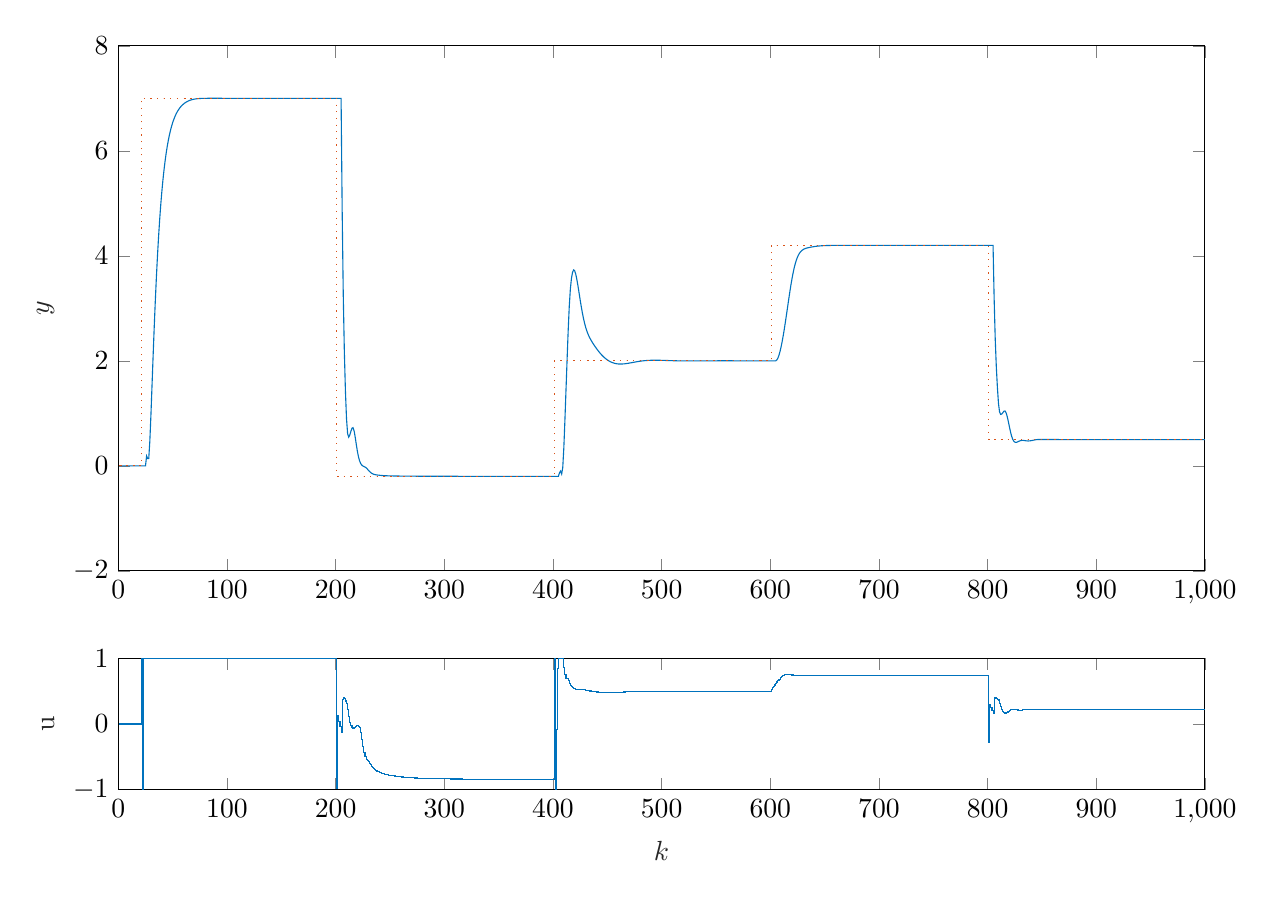
\begin{tikzpicture}

\begin{axis}[%
width=5.433in,
height=0.656in,
at={(0.854in,0.525in)},
scale only axis,
xmin=0,
xmax=1000,
xtick={0,100,200,300,400,500,600,700,800,900,1000},
xlabel style={font=\color{white!15!black}},
xlabel={$k$},
ymin=-1,
ymax=1,
ytick={-1,0,1},
ylabel style={font=\color{white!15!black}},
ylabel={u},
axis background/.style={fill=white}
]
\addplot[const plot, color=mycolor1, forget plot] table[row sep=crcr] {%
1	0\\
2	0\\
3	0\\
4	0\\
5	0\\
6	0\\
7	0\\
8	0\\
9	0\\
10	0\\
11	0\\
12	0\\
13	0\\
14	0\\
15	0\\
16	0\\
17	0\\
18	0\\
19	0\\
20	0\\
21	1\\
22	-1\\
23	1\\
24	1\\
25	1\\
26	1\\
27	1\\
28	1\\
29	1\\
30	1\\
31	1\\
32	1\\
33	1\\
34	1\\
35	1\\
36	1\\
37	1\\
38	1\\
39	1\\
40	1\\
41	1\\
42	1\\
43	1\\
44	1\\
45	1\\
46	1\\
47	1\\
48	1\\
49	1\\
50	1\\
51	1\\
52	1\\
53	1\\
54	1\\
55	1\\
56	1\\
57	0.999967792005714\\
58	0.999906795895747\\
59	0.999820555438343\\
60	0.999712178671646\\
61	0.999584391282136\\
62	0.999443255915826\\
63	0.999295235256106\\
64	0.999145755154132\\
65	0.998999427336996\\
66	0.99886022102646\\
67	0.99873116336803\\
68	0.99861422443403\\
69	0.998510479276465\\
70	0.998420275299083\\
71	0.998343349901601\\
72	0.998278965190922\\
73	0.998226060518648\\
74	0.998183384626228\\
75	0.998149598985531\\
76	0.998123361053089\\
77	0.998103389018131\\
78	0.998088506067676\\
79	0.998077666388698\\
80	0.998069967274796\\
81	0.998064650610117\\
82	0.998061096249721\\
83	0.998058809908799\\
84	0.998057407959561\\
85	0.998056600937481\\
86	0.998056177051968\\
87	0.998055986650705\\
88	0.998055928266632\\
89	0.998055936576084\\
90	0.998055972370206\\
91	0.99805601448927\\
92	0.998056053565099\\
93	0.998056087350562\\
94	0.998056117384697\\
95	0.998056146739094\\
96	0.998056178605744\\
97	0.99805621551174\\
98	0.998056258977744\\
99	0.998056309470734\\
100	0.998056366534156\\
101	0.998056429008229\\
102	0.998056495278829\\
103	0.998056563514537\\
104	0.99805663186818\\
105	0.998056698631723\\
106	0.998056762342214\\
107	0.998056821842335\\
108	0.99805687630244\\
109	0.998056925212531\\
110	0.998056968352791\\
111	0.998057005750648\\
112	0.998057037631186\\
113	0.998057064366288\\
114	0.998057086426513\\
115	0.998057104338338\\
116	0.998057118648279\\
117	0.998057129894479\\
118	0.998057138585644\\
119	0.998057145186737\\
120	0.998057150110521\\
121	0.998057153713927\\
122	0.998057156298162\\
123	0.998057158111547\\
124	0.99805715935417\\
125	0.998057160183601\\
126	0.998057160721043\\
127	0.998057161057456\\
128	0.99805716125933\\
129	0.998057161373884\\
130	0.998057161433582\\
131	0.998057161459933\\
132	0.998057161466573\\
133	0.998057161461697\\
134	0.998057161449913\\
135	0.998057161433603\\
136	0.998057161413883\\
137	0.998057161391242\\
138	0.998057161365943\\
139	0.998057161338247\\
140	0.998057161308516\\
141	0.998057161277233\\
142	0.998057161244983\\
143	0.998057161212409\\
144	0.99805716118016\\
145	0.998057161148847\\
146	0.998057161119006\\
147	0.998057161091072\\
148	0.998057161065367\\
149	0.998057161042101\\
150	0.998057161021373\\
151	0.998057161003188\\
152	0.99805716098747\\
153	0.998057160974081\\
154	0.99805716096284\\
155	0.998057160953533\\
156	0.998057160945936\\
157	0.998057160939821\\
158	0.998057160934969\\
159	0.998057160931174\\
160	0.998057160928248\\
161	0.998057160926025\\
162	0.998057160924363\\
163	0.998057160923139\\
164	0.998057160922252\\
165	0.998057160921621\\
166	0.998057160921179\\
167	0.998057160920877\\
168	0.998057160920675\\
169	0.998057160920542\\
170	0.998057160920458\\
171	0.998057160920407\\
172	0.99805716092038\\
173	0.998057160920366\\
174	0.998057160920363\\
175	0.998057160920366\\
176	0.998057160920374\\
177	0.998057160920384\\
178	0.998057160920396\\
179	0.99805716092041\\
180	0.998057160920425\\
181	0.99805716092044\\
182	0.998057160920455\\
183	0.998057160920471\\
184	0.998057160920487\\
185	0.998057160920502\\
186	0.998057160920516\\
187	0.99805716092053\\
188	0.998057160920542\\
189	0.998057160920553\\
190	0.998057160920562\\
191	0.998057160920571\\
192	0.998057160920579\\
193	0.998057160920585\\
194	0.998057160920591\\
195	0.998057160920596\\
196	0.9980571609206\\
197	0.998057160920604\\
198	0.998057160920607\\
199	0.998057160920609\\
200	0.998057160920611\\
201	-0.98557212865215\\
202	0.126816096562765\\
203	0.0429373642271256\\
204	-0.0409413681085142\\
205	-0.124820100444154\\
206	0.379955620881731\\
207	0.408036936431627\\
208	0.391419281898815\\
209	0.350864523868361\\
210	0.310100748390507\\
211	0.226360689585522\\
212	0.110965630069212\\
213	0.0280369086230579\\
214	-0.0231372708447684\\
215	-0.0565837577230117\\
216	-0.0678505859700107\\
217	-0.0537389338967414\\
218	-0.0340978473073338\\
219	-0.0235108502198887\\
220	-0.0233655387085842\\
221	-0.0358838486029105\\
222	-0.0559527666406152\\
223	-0.130170481102024\\
224	-0.235239643617944\\
225	-0.341144754839787\\
226	-0.427764776101341\\
227	-0.496559327041167\\
228	-0.538495572334973\\
229	-0.557611624124381\\
230	-0.574387641042325\\
231	-0.595553047542874\\
232	-0.619074751495959\\
233	-0.640862607201561\\
234	-0.660980005625114\\
235	-0.680119599341588\\
236	-0.696531789661496\\
237	-0.709564281004157\\
238	-0.719855332287987\\
239	-0.728513862939459\\
240	-0.736018997411208\\
241	-0.742499775699709\\
242	-0.748314178349729\\
243	-0.753719107020889\\
244	-0.758782879125262\\
245	-0.763466178176819\\
246	-0.767778456195621\\
247	-0.771775831027277\\
248	-0.775482829516149\\
249	-0.77891730394568\\
250	-0.782108446932657\\
251	-0.785093492481798\\
252	-0.78789996452363\\
253	-0.790543677682049\\
254	-0.793039256779142\\
255	-0.795400040789608\\
256	-0.797636288969862\\
257	-0.799755389859223\\
258	-0.801764167135788\\
259	-0.803669728916977\\
260	-0.805478495577497\\
261	-0.807196141123599\\
262	-0.808827919266241\\
263	-0.810378817505902\\
264	-0.811853408369155\\
265	-0.81325579044399\\
266	-0.814589746350341\\
267	-0.815858821548795\\
268	-0.817066332107327\\
269	-0.818215372150109\\
270	-0.819308852595633\\
271	-0.820349532845249\\
272	-0.82134002356034\\
273	-0.822282791327402\\
274	-0.823180170400627\\
275	-0.824034374355691\\
276	-0.824847502753839\\
277	-0.825621546511029\\
278	-0.826358395424059\\
279	-0.827059845116489\\
280	-0.827727602430555\\
281	-0.828363290036245\\
282	-0.828968451058633\\
283	-0.829544553510943\\
284	-0.830092994139752\\
285	-0.830615101958395\\
286	-0.831112141661182\\
287	-0.831585316888667\\
288	-0.832035773267117\\
289	-0.832464601250901\\
290	-0.832872838834822\\
291	-0.833261474131282\\
292	-0.833631447801308\\
293	-0.833983655351183\\
294	-0.834318949314597\\
295	-0.834638141328367\\
296	-0.834942004102315\\
297	-0.83523127329007\\
298	-0.835506649268814\\
299	-0.835768798833126\\
300	-0.836018356806265\\
301	-0.836255927572872\\
302	-0.836482086537749\\
303	-0.836697381514526\\
304	-0.836902334047449\\
305	-0.837097440669551\\
306	-0.837283174100466\\
307	-0.837459984386902\\
308	-0.837628299988496\\
309	-0.837788528811679\\
310	-0.837941059194086\\
311	-0.838086260841901\\
312	-0.838224485722388\\
313	-0.838356068913734\\
314	-0.838481329414269\\
315	-0.838600570912993\\
316	-0.838714082523267\\
317	-0.838822139481414\\
318	-0.838925003811917\\
319	-0.839022924960796\\
320	-0.839116140398695\\
321	-0.839204876195106\\
322	-0.839289347565125\\
323	-0.839369759390039\\
324	-0.839446306712993\\
325	-0.839519175210927\\
326	-0.839588541643924\\
327	-0.839654574283025\\
328	-0.839717433317571\\
329	-0.839777271243011\\
330	-0.839834233230152\\
331	-0.839888457476697\\
332	-0.839940075541946\\
333	-0.839989212665449\\
334	-0.840035988070389\\
335	-0.840080515252414\\
336	-0.840122902254623\\
337	-0.840163251929366\\
338	-0.840201662187485\\
339	-0.8402382262356\\
340	-0.840273032802018\\
341	-0.840306166351796\\
342	-0.840337707291489\\
343	-0.84036773216408\\
344	-0.840396313834539\\
345	-0.840423521666497\\
346	-0.840449421690424\\
347	-0.840474076763744\\
348	-0.84049754672326\\
349	-0.840519888530264\\
350	-0.840541156408678\\
351	-0.840561401976564\\
352	-0.840580674371321\\
353	-0.840599020368867\\
354	-0.8406164844971\\
355	-0.840633109143911\\
356	-0.840648934660008\\
357	-0.840663999456801\\
358	-0.840678340099591\\
359	-0.840691991396274\\
360	-0.840704986481793\\
361	-0.840717356898529\\
362	-0.840729132672829\\
363	-0.840740342387862\\
364	-0.84075101325297\\
365	-0.840761171169694\\
366	-0.84077084079462\\
367	-0.840780045599212\\
368	-0.840788807926765\\
369	-0.840797149046628\\
370	-0.840805089205813\\
371	-0.840812647678136\\
372	-0.840819842810984\\
373	-0.840826692069843\\
374	-0.840833212080685\\
375	-0.840839418670315\\
376	-0.840845326904785\\
377	-0.840850951125956\\
378	-0.840856304986303\\
379	-0.840861401482056\\
380	-0.840866252984738\\
381	-0.840870871271191\\
382	-0.840875267552162\\
383	-0.840879452499512\\
384	-0.840883436272116\\
385	-0.840887228540525\\
386	-0.840890838510431\\
387	-0.840894274945018\\
388	-0.840897546186228\\
389	-0.84090066017501\\
390	-0.840903624470595\\
391	-0.840906446268845\\
392	-0.840909132419717\\
393	-0.840911689443892\\
394	-0.840914123548601\\
395	-0.840916440642695\\
396	-0.840918646350983\\
397	-0.840920746027891\\
398	-0.840922744770455\\
399	-0.840924647430694\\
400	-0.840926458627389\\
401	1\\
402	-1\\
403	-0.0793932205941683\\
404	0.841213633916164\\
405	1\\
406	1\\
407	1\\
408	1\\
409	1\\
410	0.861460985010868\\
411	0.750208105369091\\
412	0.700785706737252\\
413	0.696828785961932\\
414	0.658203096031182\\
415	0.615588413368247\\
416	0.589964656617092\\
417	0.572908289553187\\
418	0.556233814261441\\
419	0.542978843574325\\
420	0.5353343544939\\
421	0.531020011921743\\
422	0.528203186323802\\
423	0.526693471041861\\
424	0.526149489583171\\
425	0.525805698700792\\
426	0.52520742780348\\
427	0.524262727923919\\
428	0.522438731270491\\
429	0.519746646856368\\
430	0.516543602010364\\
431	0.513110768071084\\
432	0.509634479885459\\
433	0.506261243966871\\
434	0.503087904459533\\
435	0.500155504559755\\
436	0.497471522471108\\
437	0.495029015418908\\
438	0.492815339895394\\
439	0.490816840143057\\
440	0.489021655268872\\
441	0.487420412464503\\
442	0.486005665263111\\
443	0.484771058686543\\
444	0.483710619265176\\
445	0.482818260798415\\
446	0.482087503256726\\
447	0.481511526245672\\
448	0.481112452997657\\
449	0.480874969177946\\
450	0.480784035807237\\
451	0.480824955215192\\
452	0.480983424748375\\
453	0.4812453653952\\
454	0.481596952099527\\
455	0.482024729409215\\
456	0.48251572444628\\
457	0.483057549087343\\
458	0.48363848698108\\
459	0.484247564310135\\
460	0.484874604242162\\
461	0.48551026577567\\
462	0.486146068114382\\
463	0.486774401896963\\
464	0.487388528675316\\
465	0.487982570030343\\
466	0.488551487670928\\
467	0.489091055797315\\
468	0.489597826934348\\
469	0.490069092359406\\
470	0.490502838167976\\
471	0.490897697939011\\
472	0.491252902883687\\
473	0.491568230285626\\
474	0.491843950968292\\
475	0.492080776456105\\
476	0.492279806429712\\
477	0.492442477012589\\
478	0.492570510365436\\
479	0.492665866006599\\
480	0.492730694220613\\
481	0.492767291863076\\
482	0.492778060818125\\
483	0.492765469314993\\
484	0.492732016262461\\
485	0.492680198714579\\
486	0.492612482538043\\
487	0.492531276311148\\
488	0.492438908446556\\
489	0.492337607495353\\
490	0.492229485558171\\
491	0.492116524700746\\
492	0.492000566246166\\
493	0.491883302794407\\
494	0.49176627280152\\
495	0.491650857536114\\
496	0.491538280219331\\
497	0.491429607146513\\
498	0.491325750583757\\
499	0.491227473230661\\
500	0.49113539404134\\
501	0.491049995199166\\
502	0.490971630046285\\
503	0.490900531776581\\
504	0.490836822710105\\
505	0.49078052397772\\
506	0.490731565456652\\
507	0.490689795810415\\
508	0.49065499249997\\
509	0.490626871646764\\
510	0.490605097642209\\
511	0.490589292411991\\
512	0.490579044257231\\
513	0.490573916207711\\
514	0.490573453835024\\
515	0.490577192485548\\
516	0.490584663904367\\
517	0.490595402231745\\
518	0.490608949363336\\
519	0.490624859673992\\
520	0.49064270411284\\
521	0.490662073684153\\
522	0.490682582334505\\
523	0.490703869271831\\
524	0.490725600746205\\
525	0.490747471325648\\
526	0.490769204702907\\
527	0.490790554071146\\
528	0.49081130210777\\
529	0.490831260606311\\
530	0.490850269796439\\
531	0.490868197391839\\
532	0.490884937404866\\
533	0.490900408765768\\
534	0.490914553782725\\
535	0.490927336477219\\
536	0.490938740827206\\
537	0.490948768948399\\
538	0.490957439241645\\
539	0.490964784531961\\
540	0.490970850222303\\
541	0.490975692482661\\
542	0.490979376492577\\
543	0.490981974752707\\
544	0.490983565478683\\
545	0.490984231088196\\
546	0.490984056790025\\
547	0.490983129281642\\
548	0.490981535560047\\
549	0.490979361848704\\
550	0.490976692641727\\
551	0.49097360986499\\
552	0.49097019215244\\
553	0.490966514234707\\
554	0.490962646436042\\
555	0.490958654274712\\
556	0.490954598161252\\
557	0.490950533188333\\
558	0.49094650900556\\
559	0.490942569772155\\
560	0.490938754180252\\
561	0.490935095541433\\
562	0.490931621929076\\
563	0.490928356369228\\
564	0.490925317072784\\
565	0.49092251770207\\
566	0.490919967665129\\
567	0.490917672431425\\
568	0.490915633862983\\
569	0.490913850555468\\
570	0.490912318184085\\
571	0.490911029849679\\
572	0.490909976420849\\
573	0.490909146868383\\
574	0.490908528588757\\
575	0.490908107713945\\
576	0.490907869405168\\
577	0.490907798128703\\
578	0.490907877912237\\
579	0.490908092580649\\
580	0.490908425970473\\
581	0.490908862122607\\
582	0.490909385453159\\
583	0.490909980902568\\
584	0.490910634063422\\
585	0.490911331287564\\
586	0.490912059773304\\
587	0.49091280763369\\
588	0.490913563946924\\
589	0.490914318790131\\
590	0.490915063257731\\
591	0.49091578946577\\
592	0.490916490543556\\
593	0.490917160613981\\
594	0.490917794763919\\
595	0.490918389006031\\
596	0.490918940233329\\
597	0.490919446167743\\
598	0.490919905303945\\
599	0.490920316849549\\
600	0.490920680662797\\
601	0.528625797495277\\
602	0.550117944729166\\
603	0.572783452054588\\
604	0.595448916305809\\
605	0.618114339636402\\
606	0.640511987523558\\
607	0.662404880323587\\
608	0.68332692758249\\
609	0.702658112570154\\
610	0.719853828618662\\
611	0.734395521755186\\
612	0.745816406340412\\
613	0.753741509314692\\
614	0.757946485750611\\
615	0.758622981802054\\
616	0.757851737847452\\
617	0.755976389643343\\
618	0.753390805651018\\
619	0.750523726090453\\
620	0.747792052083101\\
621	0.745379973048655\\
622	0.743369391810211\\
623	0.741808177459646\\
624	0.740698667805817\\
625	0.739994634267995\\
626	0.739627270174433\\
627	0.739523869173265\\
628	0.739612520416681\\
629	0.739826070196565\\
630	0.740107428645348\\
631	0.740412079973015\\
632	0.740707646726257\\
633	0.740972651490449\\
634	0.741195073490093\\
635	0.741370470841659\\
636	0.741499897837446\\
637	0.741588021603428\\
638	0.741641566974719\\
639	0.741668069306021\\
640	0.741674940585105\\
641	0.741668850844393\\
642	0.74165538064101\\
643	0.741638881359965\\
644	0.741622488285647\\
645	0.741608238554639\\
646	0.74159724982769\\
647	0.741589923264986\\
648	0.741586144769641\\
649	0.741585467327167\\
650	0.741587264164804\\
651	0.741590848255535\\
652	0.741595558264607\\
653	0.741600814060995\\
654	0.741606146611527\\
655	0.741611207821967\\
656	0.741615765922806\\
657	0.741619691504743\\
658	0.741622938504191\\
659	0.741625523508951\\
660	0.741627505821896\\
661	0.741628969866389\\
662	0.741630010793458\\
663	0.741630723582735\\
664	0.741631195517923\\
665	0.741631501649164\\
666	0.741631702707605\\
667	0.741631844886118\\
668	0.74163196091847\\
669	0.741632071952945\\
670	0.741632189805392\\
671	0.741632319274587\\
672	0.741632460298053\\
673	0.741632609811256\\
674	0.741632763243117\\
675	0.741632915634457\\
676	0.741633062403731\\
677	0.741633199807855\\
678	0.741633325157685\\
679	0.741633436850256\\
680	0.741633534276169\\
681	0.741633617652692\\
682	0.741633687823345\\
683	0.741633746054424\\
684	0.741633793849223\\
685	0.74163383279225\\
686	0.741633864428926\\
687	0.741633890181164\\
688	0.741633911295727\\
689	0.741633928820202\\
690	0.741633943600506\\
691	0.741633956293769\\
692	0.741633967390958\\
693	0.741633977244482\\
694	0.741633986097031\\
695	0.741633994108986\\
696	0.74163400138261\\
697	0.741634007982159\\
698	0.741634013949564\\
699	0.741634019315903\\
700	0.74163402410912\\
701	0.741634028358636\\
702	0.741634032097556\\
703	0.741634035363144\\
704	0.741634038196167\\
705	0.741634040639616\\
706	0.741634042737178\\
707	0.74163404453174\\
708	0.741634046064099\\
709	0.741634047371979\\
710	0.741634048489375\\
711	0.74163404944622\\
712	0.741634050268318\\
713	0.741634050977515\\
714	0.741634051592003\\
715	0.741634052126742\\
716	0.741634052593908\\
717	0.741634053003365\\
718	0.741634053363093\\
719	0.741634053679587\\
720	0.74163405395818\\
721	0.741634054203329\\
722	0.741634054418822\\
723	0.741634054607948\\
724	0.741634054773606\\
725	0.741634054918399\\
726	0.74163405504468\\
727	0.74163405515459\\
728	0.741634055250077\\
729	0.741634055332911\\
730	0.741634055404692\\
731	0.741634055466855\\
732	0.741634055520676\\
733	0.741634055567285\\
734	0.741634055607673\\
735	0.741634055642699\\
736	0.741634055673108\\
737	0.741634055699539\\
738	0.741634055722539\\
739	0.741634055742576\\
740	0.741634055760047\\
741	0.741634055775293\\
742	0.741634055788602\\
743	0.741634055800224\\
744	0.741634055810374\\
745	0.741634055819235\\
746	0.741634055826969\\
747	0.741634055833716\\
748	0.741634055839597\\
749	0.741634055844721\\
750	0.741634055849183\\
751	0.741634055853067\\
752	0.741634055856445\\
753	0.741634055859383\\
754	0.741634055861937\\
755	0.741634055864157\\
756	0.741634055866087\\
757	0.741634055867765\\
758	0.741634055869225\\
759	0.741634055870495\\
760	0.7416340558716\\
761	0.741634055872561\\
762	0.741634055873399\\
763	0.741634055874128\\
764	0.741634055874763\\
765	0.741634055875317\\
766	0.741634055875799\\
767	0.74163405587622\\
768	0.741634055876586\\
769	0.741634055876905\\
770	0.741634055877183\\
771	0.741634055877425\\
772	0.741634055877635\\
773	0.741634055877819\\
774	0.741634055877978\\
775	0.741634055878118\\
776	0.741634055878239\\
777	0.741634055878344\\
778	0.741634055878436\\
779	0.741634055878516\\
780	0.741634055878586\\
781	0.741634055878646\\
782	0.741634055878699\\
783	0.741634055878745\\
784	0.741634055878785\\
785	0.74163405587882\\
786	0.74163405587885\\
787	0.741634055878876\\
788	0.741634055878899\\
789	0.74163405587892\\
790	0.741634055878937\\
791	0.741634055878952\\
792	0.741634055878965\\
793	0.741634055878977\\
794	0.741634055878987\\
795	0.741634055878995\\
796	0.741634055879003\\
797	0.74163405587901\\
798	0.741634055879016\\
799	0.741634055879021\\
800	0.741634055879025\\
801	-0.277730995706974\\
802	0.293912953361805\\
803	0.250808604800437\\
804	0.207704256239069\\
805	0.1645999076777\\
806	0.400157868139949\\
807	0.397237719927082\\
808	0.386180217460633\\
809	0.371225694052644\\
810	0.36617385316509\\
811	0.31542799635836\\
812	0.261055078562572\\
813	0.222536471430091\\
814	0.195196069119405\\
815	0.17308723221437\\
816	0.16443965568716\\
817	0.170361692458966\\
818	0.182857624970205\\
819	0.196205734022884\\
820	0.208704190697366\\
821	0.218221709888399\\
822	0.223987205711233\\
823	0.225862000738032\\
824	0.224898781560209\\
825	0.222130613046459\\
826	0.218573559066019\\
827	0.215172770317229\\
828	0.21268757456123\\
829	0.21148650446655\\
830	0.211595241505673\\
831	0.212816677421126\\
832	0.214808830951621\\
833	0.217156902884548\\
834	0.219470264550704\\
835	0.221452401565837\\
836	0.222922335115883\\
837	0.223812188289467\\
838	0.224154828795152\\
839	0.224057565286481\\
840	0.223666441259918\\
841	0.223133309908714\\
842	0.222591227386746\\
843	0.222138037735572\\
844	0.221828864865013\\
845	0.221677926290332\\
846	0.22166715491314\\
847	0.221757916838492\\
848	0.2219030898205\\
849	0.222057606297311\\
850	0.222185987677029\\
851	0.222266219811547\\
852	0.222290283520976\\
853	0.222262161595542\\
854	0.222194272987159\\
855	0.222103307822324\\
856	0.222006338228113\\
857	0.221917813885828\\
858	0.221847730542254\\
859	0.221800992995092\\
860	0.221777794678614\\
861	0.221774702808717\\
862	0.221786089204343\\
863	0.221805578555849\\
864	0.221827266331468\\
865	0.221846558028848\\
866	0.221860581559988\\
867	0.221868209364403\\
868	0.22186978401324\\
869	0.221866667385256\\
870	0.221860733216935\\
871	0.221853902784158\\
872	0.221847791440094\\
873	0.22184349803712\\
874	0.221841537071901\\
875	0.221841889282801\\
876	0.22184413236893\\
877	0.221847609407809\\
878	0.221851596706657\\
879	0.221855442461769\\
880	0.221858659692781\\
881	0.221860968808331\\
882	0.221862294890623\\
883	0.221862731238008\\
884	0.221862483591844\\
885	0.2218618091954\\
886	0.22186096222343\\
887	0.221860153199447\\
888	0.221859525772857\\
889	0.221859150461158\\
890	0.221859032194306\\
891	0.221859126950918\\
892	0.221859362409124\\
893	0.221859658118632\\
894	0.221859941900477\\
895	0.221860160640473\\
896	0.221860285049868\\
897	0.221860309096525\\
898	0.221860245539481\\
899	0.221860119304804\\
900	0.221859960374842\\
901	0.221859797529686\\
902	0.22185965380179\\
903	0.221859543999304\\
904	0.221859474213307\\
905	0.221859442907445\\
906	0.221859443018504\\
907	0.221859464465692\\
908	0.221859496545524\\
909	0.221859529837506\\
910	0.221859557421069\\
911	0.221859575369888\\
912	0.221859582620144\\
913	0.221859580391137\\
914	0.221859571367914\\
915	0.221859558843711\\
916	0.221859545977493\\
917	0.221859535263725\\
918	0.221859528251251\\
919	0.221859525496738\\
920	0.221859526701898\\
921	0.221859530965116\\
922	0.221859537075949\\
923	0.221859543791426\\
924	0.221859550051378\\
925	0.221859555111\\
926	0.221859558588347\\
927	0.221859560439495\\
928	0.22185956088328\\
929	0.221859560300642\\
930	0.221859559131785\\
931	0.221859557788982\\
932	0.221859556595806\\
933	0.221859555756466\\
934	0.221859555352895\\
935	0.221859555363169\\
936	0.221859555692793\\
937	0.221859556210353\\
938	0.221859556780381\\
939	0.221859557288572\\
940	0.221859557656955\\
941	0.221859557848971\\
942	0.221859557866105\\
943	0.221859557738751\\
944	0.221859557514324\\
945	0.221859557245311\\
946	0.221859556979345\\
947	0.221859556752479\\
948	0.221859556586034\\
949	0.221859556486677\\
950	0.221859556448921\\
951	0.221859556459048\\
952	0.22185955649942\\
953	0.221859556552383\\
954	0.22185955660319\\
955	0.221859556641704\\
956	0.221859556662898\\
957	0.221859556666362\\
958	0.221859556655159\\
959	0.221859556634375\\
960	0.2218595566097\\
961	0.221859556586257\\
962	0.221859556567829\\
963	0.221859556556513\\
964	0.221859556552747\\
965	0.221859556555623\\
966	0.221859556563353\\
967	0.221859556573772\\
968	0.221859556584788\\
969	0.221859556594709\\
970	0.221859556602424\\
971	0.221859556607444\\
972	0.221859556609827\\
973	0.221859556610034\\
974	0.22185955660875\\
975	0.221859556606715\\
976	0.221859556604586\\
977	0.221859556602848\\
978	0.221859556601778\\
979	0.221859556601454\\
980	0.22185955660179\\
981	0.221859556602595\\
982	0.221859556603638\\
983	0.221859556604692\\
984	0.22185955660558\\
985	0.22185955660619\\
986	0.221859556606481\\
987	0.221859556606475\\
988	0.221859556606235\\
989	0.221859556605848\\
990	0.221859556605404\\
991	0.22185955660498\\
992	0.221859556604632\\
993	0.221859556604389\\
994	0.221859556604257\\
995	0.221859556604221\\
996	0.221859556604256\\
997	0.221859556604332\\
998	0.221859556604419\\
999	0.221859556604496\\
1000	0.221859556604549\\
};
\end{axis}

\begin{axis}[%
width=5.433in,
height=2.625in,
at={(0.854in,1.619in)},
scale only axis,
xmin=0,
xmax=1000,
xtick={0,100,200,300,400,500,600,700,800,900,1000},
ymin=-2,
ymax=8,
ytick={-2,0,2,4,6,8},
ylabel style={font=\color{white!15!black}},
ylabel={$y$},
axis background/.style={fill=white}
]
\addplot [color=mycolor1, forget plot]
  table[row sep=crcr]{%
1	0\\
2	0\\
3	0\\
4	0\\
5	0\\
6	0\\
7	0\\
8	0\\
9	0\\
10	0\\
11	0\\
12	0\\
13	0\\
14	0\\
15	0\\
16	0\\
17	0\\
18	0\\
19	0\\
20	0\\
21	0\\
22	0\\
23	0\\
24	0\\
25	0\\
26	0.187021166666667\\
27	0.1388412867175\\
28	0.140250690946808\\
29	0.474484324849734\\
30	0.969546331063805\\
31	1.52616259558225\\
32	2.0885485281946\\
33	2.626753768434\\
34	3.12601990380585\\
35	3.58038393470303\\
36	3.98884990759164\\
37	4.35311200695019\\
38	4.67621316346153\\
39	4.9617662410529\\
40	5.21351218539529\\
41	5.43507880520345\\
42	5.62985795429437\\
43	5.80095163977713\\
44	5.95115740202629\\
45	6.08297529098591\\
46	6.19862599114077\\
47	6.30007399804402\\
48	6.38905235869494\\
49	6.46708704494637\\
50	6.53551995075424\\
51	6.59553004318073\\
52	6.64815250657622\\
53	6.69429589177026\\
54	6.73475737322811\\
55	6.77023626060868\\
56	6.80134592719055\\
57	6.82862431828721\\
58	6.85254319521671\\
59	6.87351625883499\\
60	6.89190628351707\\
61	6.90803137914879\\
62	6.9221571561818\\
63	6.9345048807561\\
64	6.94526348334981\\
65	6.95459735979641\\
66	6.96265149037602\\
67	6.96955643533663\\
68	6.97543237470589\\
69	6.98039139530736\\
70	6.98453860470391\\
71	6.9879726710904\\
72	6.99078593221572\\
73	6.99306417508938\\
74	6.9948863004818\\
75	6.99632403668614\\
76	6.99744176799967\\
77	6.99829650681382\\
78	6.99893802783778\\
79	6.99940916071317\\
80	6.99974621621313\\
81	6.99997951353735\\
82	7.00013397569175\\
83	7.00022976068341\\
84	7.00028289884826\\
85	7.00030591161241\\
86	7.00030839287583\\
87	7.00029753980915\\
88	7.00027862495347\\
89	7.00025540602186\\
90	7.00023047349442\\
91	7.00020553887543\\
92	7.00018166841368\\
93	7.00015946828966\\
94	7.00013922785523\\
95	7.00012102759434\\
96	7.0001048181887\\
97	7.00009047653904\\
98	7.00007784390936\\
99	7.00006675060903\\
100	7.00005703086864\\
101	7.00004853084565\\
102	7.00004111204475\\
103	7.00003465187109\\
104	7.00002904256012\\
105	7.00002418934281\\
106	7.00002000840512\\
107	7.0000164249744\\
108	7.00001337170301\\
109	7.00001078740873\\
110	7.00000861616136\\
111	7.00000680666561\\
112	7.00000531187304\\
113	7.00000408875293\\
114	7.00000309815896\\
115	7.00000230473974\\
116	7.00000167685456\\
117	7.0000011864689\\
118	7.00000080901528\\
119	7.00000052321473\\
120	7.00000031086074\\
121	7.00000015657224\\
122	7.00000004752475\\
123	6.99999997316982\\
124	6.99999992495278\\
125	6.99999989603735\\
126	6.99999988104468\\
127	6.99999987581205\\
128	6.99999987717502\\
129	6.9999998827749\\
130	6.99999989089225\\
131	6.99999990030561\\
132	6.99999991017405\\
133	6.99999991994143\\
134	6.99999992925994\\
135	6.99999993793013\\
136	6.99999994585509\\
137	6.99999995300612\\
138	6.99999995939768\\
139	6.99999996506965\\
140	6.9999999700752\\
141	6.99999997447284\\
142	6.99999997832141\\
143	6.99999998167729\\
144	6.99999998459295\\
145	6.99999998711645\\
146	6.9999999892914\\
147	6.99999999115726\\
148	6.99999999274972\\
149	6.99999999410112\\
150	6.99999999524078\\
151	6.99999999619533\\
152	6.99999999698892\\
153	6.99999999764344\\
154	6.99999999817861\\
155	6.99999999861215\\
156	6.99999999895987\\
157	6.99999999923574\\
158	6.99999999945204\\
159	6.99999999961943\\
160	6.99999999974709\\
161	6.99999999984284\\
162	6.99999999991327\\
163	6.99999999996385\\
164	6.9999999999991\\
165	7.00000000002269\\
166	7.00000000003756\\
167	7.00000000004603\\
168	7.00000000004993\\
169	7.00000000005065\\
170	7.00000000004925\\
171	7.00000000004651\\
172	7.00000000004299\\
173	7.00000000003909\\
174	7.00000000003511\\
175	7.00000000003121\\
176	7.00000000002751\\
177	7.00000000002407\\
178	7.00000000002094\\
179	7.00000000001812\\
180	7.00000000001559\\
181	7.00000000001336\\
182	7.00000000001139\\
183	7.00000000000966\\
184	7.00000000000815\\
185	7.00000000000685\\
186	7.00000000000572\\
187	7.00000000000474\\
188	7.00000000000391\\
189	7.00000000000321\\
190	7.00000000000261\\
191	7.00000000000211\\
192	7.00000000000169\\
193	7.00000000000134\\
194	7.00000000000105\\
195	7.00000000000082\\
196	7.00000000000062\\
197	7.00000000000047\\
198	7.00000000000034\\
199	7.00000000000025\\
200	7.00000000000017\\
201	7.00000000000011\\
202	7.00000000000007\\
203	7.00000000000004\\
204	7.00000000000002\\
205	7\\
206	4.86335476661778\\
207	3.25877503965814\\
208	2.17426882188505\\
209	1.42137030951934\\
210	0.895123794698472\\
211	0.614020737914612\\
212	0.546688791774948\\
213	0.585635292728324\\
214	0.656169417152532\\
215	0.71534122313945\\
216	0.727276968889237\\
217	0.664795951061379\\
218	0.545102069280059\\
219	0.406540150556953\\
220	0.277662070154241\\
221	0.172625845961643\\
222	0.0957263213571883\\
223	0.045123839783349\\
224	0.0149386017527383\\
225	-0.00218299529340794\\
226	-0.0130824020464863\\
227	-0.022725335486353\\
228	-0.0367049885316046\\
229	-0.057534195119162\\
230	-0.0816210196595944\\
231	-0.104651114506785\\
232	-0.124221472297342\\
233	-0.139941445428623\\
234	-0.151895090390063\\
235	-0.160341518983345\\
236	-0.166192052029197\\
237	-0.170469599689313\\
238	-0.173882188539503\\
239	-0.176746526931804\\
240	-0.179223520188287\\
241	-0.181431356907662\\
242	-0.183395408711423\\
243	-0.18509782911998\\
244	-0.186535725090978\\
245	-0.187741290299746\\
246	-0.188756665278354\\
247	-0.189616178880755\\
248	-0.190352713042006\\
249	-0.190996540091709\\
250	-0.191570666850053\\
251	-0.19208907722698\\
252	-0.192560429125756\\
253	-0.192991560320609\\
254	-0.193387675948417\\
255	-0.193752655018943\\
256	-0.194089796440725\\
257	-0.194402339768207\\
258	-0.194693303543046\\
259	-0.194965201658787\\
260	-0.195220117956378\\
261	-0.195459811892504\\
262	-0.195685747837976\\
263	-0.19589910825301\\
264	-0.196100863529502\\
265	-0.196291853681568\\
266	-0.196472820960568\\
267	-0.196644423648872\\
268	-0.19680725178323\\
269	-0.196961842778287\\
270	-0.19710868836159\\
271	-0.197248236478451\\
272	-0.197380896144022\\
273	-0.197507043429338\\
274	-0.197627026043619\\
275	-0.19774116653449\\
276	-0.197849765369563\\
277	-0.197953103937679\\
278	-0.198051446717182\\
279	-0.198145042796811\\
280	-0.19823412716045\\
281	-0.198318921865375\\
282	-0.198399637030736\\
283	-0.19847647164554\\
284	-0.198549614309431\\
285	-0.19861924392764\\
286	-0.198685530335339\\
287	-0.198748634847819\\
288	-0.19880871075868\\
289	-0.19886590379964\\
290	-0.198920352559763\\
291	-0.198972188867592\\
292	-0.199021538144638\\
293	-0.199068519736089\\
294	-0.199113247220397\\
295	-0.199155828699082\\
296	-0.199196367069407\\
297	-0.199234960281851\\
298	-0.199271701583328\\
299	-0.199306679746978\\
300	-0.199339979289634\\
301	-0.199371680677977\\
302	-0.199401860524103\\
303	-0.199430591771132\\
304	-0.199457943869513\\
305	-0.199483982944615\\
306	-0.199508771956097\\
307	-0.199532370849496\\
308	-0.199554836700453\\
309	-0.199576223851968\\
310	-0.199596584045047\\
311	-0.19961596654307\\
312	-0.199634418250192\\
313	-0.199651983824078\\
314	-0.199668705783247\\
315	-0.199684624609298\\
316	-0.199699778844248\\
317	-0.199714205183237\\
318	-0.199727938562807\\
319	-0.199741012244982\\
320	-0.199753457897332\\
321	-0.19976530566923\\
322	-0.199776584264469\\
323	-0.19978732101042\\
324	-0.199797541923894\\
325	-0.199807271773862\\
326	-0.199816534141187\\
327	-0.199825351475504\\
328	-0.199833745149385\\
329	-0.199841735509921\\
330	-0.199849341927847\\
331	-0.199856582844307\\
332	-0.199863475815401\\
333	-0.199870037554595\\
334	-0.199876283973103\\
335	-0.199882230218349\\
336	-0.199887890710578\\
337	-0.199893279177722\\
338	-0.1998984086886\\
339	-0.199903291684526\\
340	-0.199907940009407\\
341	-0.199912364938397\\
342	-0.199916577205185\\
343	-0.19992058702797\\
344	-0.199924404134196\\
345	-0.199928037784104\\
346	-0.199931496793149\\
347	-0.199934789553349\\
348	-0.199937924053608\\
349	-0.199940907899069\\
350	-0.199943748329532\\
351	-0.199946452236995\\
352	-0.199949026182353\\
353	-0.199951476411295\\
354	-0.199953808869437\\
355	-0.199956029216734\\
356	-0.199958142841196\\
357	-0.19996015487195\\
358	-0.199962070191671\\
359	-0.199963893448417\\
360	-0.199965629066903\\
361	-0.199967281259224\\
362	-0.199968854035071\\
363	-0.199970351211452\\
364	-0.199971776421946\\
365	-0.199973133125521\\
366	-0.199974424614917\\
367	-0.199975654024633\\
368	-0.199976824338531\\
369	-0.199977938397072\\
370	-0.199978998904206\\
371	-0.199980008433934\\
372	-0.199980969436545\\
373	-0.199981884244569\\
374	-0.199982755078428\\
375	-0.199983584051828\\
376	-0.199984373176883\\
377	-0.199985124369\\
378	-0.199985839451526\\
379	-0.199986520160171\\
380	-0.199987168147217\\
381	-0.199987784985533\\
382	-0.199988372172388\\
383	-0.199988931133082\\
384	-0.19998946322441\\
385	-0.19998996973795\\
386	-0.1999904519032\\
387	-0.19999091089056\\
388	-0.199991347814173\\
389	-0.199991763734628\\
390	-0.199992159661535\\
391	-0.199992536555976\\
392	-0.199992895332835\\
393	-0.199993236863018\\
394	-0.199993561975573\\
395	-0.199993871459692\\
396	-0.199994166066635\\
397	-0.199994446511549\\
398	-0.199994713475206\\
399	-0.199994967605654\\
400	-0.199995209519788\\
401	-0.199995439804852\\
402	-0.199995659019861\\
403	-0.199995867696957\\
404	-0.199996066342705\\
405	-0.199996255439317\\
406	-0.132163785060861\\
407	-0.100138416940354\\
408	-0.155792752809765\\
409	-0.0337510462703135\\
410	0.348740310348135\\
411	0.875562431198992\\
412	1.4536251516521\\
413	2.03093274194096\\
414	2.57986621523138\\
415	3.04107045985266\\
416	3.36819346620131\\
417	3.5695264244179\\
418	3.6850995820833\\
419	3.73165471328807\\
420	3.71425412547092\\
421	3.64693209842902\\
422	3.5469151497671\\
423	3.42666571410064\\
424	3.29579414803766\\
425	3.16332402990744\\
426	3.03641512562332\\
427	2.91948386341055\\
428	2.81486975705767\\
429	2.72349112615647\\
430	2.64507380310164\\
431	2.57845484915516\\
432	2.52201330953883\\
433	2.47377038075358\\
434	2.43164878985822\\
435	2.39383698663308\\
436	2.35896294621312\\
437	2.32609454239772\\
438	2.29467616161102\\
439	2.264441613256\\
440	2.23531756698881\\
441	2.20733860042989\\
442	2.18058606421927\\
443	2.15514992337437\\
444	2.13110815420757\\
445	2.1085182719323\\
446	2.08741618015973\\
447	2.06781856274012\\
448	2.04972639301356\\
449	2.0331283005981\\
450	2.0180032995398\\
451	2.0043228051143\\
452	1.99205213064794\\
453	1.98116420152477\\
454	1.97163363744492\\
455	1.96342880190176\\
456	1.95650872393106\\
457	1.95082265145918\\
458	1.94631083977341\\
459	1.94290585293955\\
460	1.94053405057526\\
461	1.93911709718839\\
462	1.93857340929954\\
463	1.93881949769018\\
464	1.93977118520179\\
465	1.94134469324587\\
466	1.94345759721166\\
467	1.94602965483185\\
468	1.94898351366383\\
469	1.95224530491395\\
470	1.95574513129699\\
471	1.95941745672961\\
472	1.963201405553\\
473	1.96704097875944\\
474	1.97088519441963\\
475	1.97468815920744\\
476	1.97840907762162\\
477	1.98201220521907\\
478	1.98546675191034\\
479	1.9887467411234\\
480	1.99183083041535\\
481	1.99470209889866\\
482	1.99734780664357\\
483	1.99975913101578\\
484	2.00193088470235\\
485	2.00386121996569\\
486	2.00555132343909\\
487	2.00700510553764\\
488	2.00822888830112\\
489	2.00923109521187\\
490	2.01002194624063\\
491	2.01061316106797\\
492	2.01101767311183\\
493	2.0112493566649\\
494	2.01132276911311\\
495	2.01125290987291\\
496	2.01105499735393\\
497	2.01074426492909\\
498	2.01033577658172\\
499	2.00984426260048\\
500	2.00928397541323\\
501	2.00866856539222\\
502	2.00801097622803\\
503	2.00732335925987\\
504	2.00661700596718\\
505	2.0059022976716\\
506	2.00518867137024\\
507	2.00448460051964\\
508	2.00379758951431\\
509	2.00313418055315\\
510	2.00249997155887\\
511	2.00189964380907\\
512	2.00133699794993\\
513	2.00081499709224\\
514	2.00033581573369\\
515	1.99990089330673\\
516	1.99951099121805\\
517	1.99916625231925\\
518	1.99886626182897\\
519	1.99861010881065\\
520	1.99839644739739\\
521	1.99822355704288\\
522	1.9980894011653\\
523	1.99799168363708\\
524	1.99792790265694\\
525	1.99789540162143\\
526	1.99789141668929\\
527	1.99791312080429\\
528	1.99795766400912\\
529	1.99802220994521\\
530	1.99810396848981\\
531	1.99820022453308\\
532	1.99830836294376\\
533	1.99842588981239\\
534	1.99855045009632\\
535	1.99867984182074\\
536	1.99881202701516\\
537	1.99894513958513\\
538	1.99907749033515\\
539	1.99920756937042\\
540	1.9993340461133\\
541	1.99945576717443\\
542	1.99957175232014\\
543	1.99968118877556\\
544	1.99978342409879\\
545	1.99987795785468\\
546	1.99996443230806\\
547	2.00004262234602\\
548	2.00011242482675\\
549	2.00017384753981\\
550	2.0002269979486\\
551	2.0002720718713\\
552	2.00030934224199\\
553	2.00033914807805\\
554	2.00036188376529\\
555	2.00037798875705\\
556	2.0003879377691\\
557	2.00039223153807\\
558	2.00039138819731\\
559	2.00038593531185\\
560	2.0003764026015\\
561	2.00036331537028\\
562	2.00034718865004\\
563	2.00032852205674\\
564	2.00030779534939\\
565	2.00028546467428\\
566	2.00026195947077\\
567	2.00023768000908\\
568	2.00021299552603\\
569	2.00018824292108\\
570	2.00016372597169\\
571	2.0001397150253\\
572	2.00011644712353\\
573	2.00009412651361\\
574	2.00007292550183\\
575	2.00005298560439\\
576	2.00003441895172\\
577	2.000017309904\\
578	2.00000171683715\\
579	1.99998767406056\\
580	1.99997519383048\\
581	1.99996426842499\\
582	1.99995487224966\\
583	1.99994696394543\\
584	1.99994048847316\\
585	1.99993537915224\\
586	1.99993155963348\\
587	1.99992894578906\\
588	1.99992744750545\\
589	1.99992697036732\\
590	1.99992741722352\\
591	1.99992868962795\\
592	1.99993068915082\\
593	1.99993331855759\\
594	1.99993648285477\\
595	1.99994009020351\\
596	1.99994405270322\\
597	1.99994828704908\\
598	1.99995271506816\\
599	1.99995726414\\
600	1.99996186750816\\
601	1.99996646449015\\
602	1.9999710005933\\
603	1.99997542754476\\
604	1.99997970324384\\
605	1.9999837916452\\
606	2.01560958036657\\
607	2.05177993790585\\
608	2.10763777097945\\
609	2.18160619684844\\
610	2.27176542180749\\
611	2.37610512339555\\
612	2.49261233858188\\
613	2.61921801593157\\
614	2.75366706010912\\
615	2.89345263014702\\
616	3.0358004738978\\
617	3.17768187832243\\
618	3.31586041313217\\
619	3.44698465968026\\
620	3.56781854218411\\
621	3.67617705980507\\
622	3.77097274783823\\
623	3.8519495490629\\
624	3.91952889589898\\
625	3.97469925577883\\
626	4.01883121194312\\
627	4.05348198907276\\
628	4.08025263421352\\
629	4.10068565426157\\
630	4.11618649783154\\
631	4.12797288748364\\
632	4.13705378321988\\
633	4.14423001829349\\
634	4.15010872251003\\
635	4.15512702700824\\
636	4.15958110803114\\
637	4.16365649868106\\
638	4.16745669227531\\
639	4.17102838819597\\
640	4.17438250819697\\
641	4.17751062887591\\
642	4.18039697101796\\
643	4.18302644811059\\
644	4.18538944342277\\
645	4.18748403149037\\
646	4.18931634407046\\
647	4.1908997133923\\
648	4.19225312054678\\
649	4.19339935905257\\
650	4.1943632102239\\
651	4.19516982497005\\
652	4.19584342031796\\
653	4.19640633132353\\
654	4.19687841038089\\
655	4.19727673422436\\
656	4.19761556134841\\
657	4.19790647618686\\
658	4.19815865815395\\
659	4.19837922070683\\
660	4.19857357554694\\
661	4.19874578808161\\
662	4.19889890096282\\
663	4.19903521201178\\
664	4.19915650063418\\
665	4.19926420275626\\
666	4.1993595384171\\
667	4.19944359864055\\
668	4.19951739936344\\
669	4.19958191033246\\
670	4.19963806630622\\
671	4.19968676688632\\
672	4.19972887007705\\
673	4.19976518341213\\
674	4.19979645530931\\
675	4.19982336829681\\
676	4.19984653493511\\
677	4.19986649664344\\
678	4.19988372521826\\
679	4.19989862657595\\
680	4.19991154613188\\
681	4.19992277520847\\
682	4.1999325579145\\
683	4.1999410980288\\
684	4.19994856553129\\
685	4.19995510253636\\
686	4.19996082848601\\
687	4.19996584454685\\
688	4.199970237222\\
689	4.19997408123663\\
690	4.19997744178517\\
691	4.19998037624282\\
692	4.19998293544623\\
693	4.19998516464211\\
694	4.19998710419103\\
695	4.19998879009894\\
696	4.1999902544341\\
697	4.19999152567201\\
698	4.19999262899836\\
699	4.19999358658933\\
700	4.19999441787975\\
701	4.19999513982408\\
702	4.19999576715063\\
703	4.1999963126073\\
704	4.1999967871959\\
705	4.19999720039194\\
706	4.19999756034725\\
707	4.1999978740736\\
708	4.19999814760631\\
709	4.19999838614778\\
710	4.19999859419164\\
711	4.19999877562884\\
712	4.19999893383729\\
713	4.19999907175707\\
714	4.19999919195311\\
715	4.19999929666743\\
716	4.19999938786255\\
717	4.1999994672579\\
718	4.19999953636039\\
719	4.19999959649046\\
720	4.19999964880448\\
721	4.19999969431414\\
722	4.19999973390354\\
723	4.19999976834426\\
724	4.1999997983088\\
725	4.19999982438257\\
726	4.19999984707457\\
727	4.19999986682702\\
728	4.19999988402382\\
729	4.19999989899814\\
730	4.19999991203907\\
731	4.19999992339749\\
732	4.19999993329124\\
733	4.19999994190949\\
734	4.19999994941669\\
735	4.19999995595586\\
736	4.19999996165149\\
737	4.199999966612\\
738	4.19999997093187\\
739	4.19999997469349\\
740	4.1999999779687\\
741	4.19999998082014\\
742	4.19999998330248\\
743	4.19999998546338\\
744	4.19999998734441\\
745	4.19999998898178\\
746	4.19999999040707\\
747	4.19999999164777\\
748	4.19999999272783\\
749	4.19999999366809\\
750	4.19999999448669\\
751	4.19999999519939\\
752	4.19999999581994\\
753	4.19999999636026\\
754	4.19999999683075\\
755	4.19999999724045\\
756	4.1999999975972\\
757	4.19999999790786\\
758	4.19999999817838\\
759	4.19999999841394\\
760	4.19999999861906\\
761	4.19999999879766\\
762	4.19999999895318\\
763	4.19999999908858\\
764	4.19999999920647\\
765	4.19999999930911\\
766	4.19999999939848\\
767	4.19999999947628\\
768	4.19999999954402\\
769	4.19999999960299\\
770	4.19999999965434\\
771	4.19999999969904\\
772	4.19999999973796\\
773	4.19999999977184\\
774	4.19999999980135\\
775	4.19999999982704\\
776	4.1999999998494\\
777	4.19999999986887\\
778	4.19999999988583\\
779	4.19999999990059\\
780	4.19999999991345\\
781	4.19999999992464\\
782	4.19999999993438\\
783	4.19999999994287\\
784	4.19999999995026\\
785	4.19999999995669\\
786	4.19999999996229\\
787	4.19999999996717\\
788	4.19999999997141\\
789	4.19999999997511\\
790	4.19999999997832\\
791	4.19999999998113\\
792	4.19999999998357\\
793	4.19999999998569\\
794	4.19999999998754\\
795	4.19999999998915\\
796	4.19999999999056\\
797	4.19999999999178\\
798	4.19999999999284\\
799	4.19999999999377\\
800	4.19999999999457\\
801	4.19999999999527\\
802	4.19999999999588\\
803	4.19999999999641\\
804	4.19999999999688\\
805	4.19999999999728\\
806	3.18853649947522\\
807	2.4175087172272\\
808	1.8860353213932\\
809	1.49413301847216\\
810	1.18591453054249\\
811	1.02541294454903\\
812	0.979247864230476\\
813	0.986877113459269\\
814	1.01219594161775\\
815	1.03960618931602\\
816	1.04487671067905\\
817	1.01088167397873\\
818	0.94117410081411\\
819	0.849405304726777\\
820	0.74876041255457\\
821	0.652142119031302\\
822	0.570671460271265\\
823	0.510249731291203\\
824	0.471397549088857\\
825	0.451451043383566\\
826	0.446083080550003\\
827	0.45034838231874\\
828	0.459457235994192\\
829	0.469496811202168\\
830	0.477797705358616\\
831	0.482964559033025\\
832	0.48472879983737\\
833	0.483685001036387\\
834	0.480924800866386\\
835	0.477665124634476\\
836	0.474968239526137\\
837	0.473576346570458\\
838	0.473845100538849\\
839	0.475761516987601\\
840	0.479024852005094\\
841	0.483158086241955\\
842	0.487621730345729\\
843	0.491912780368976\\
844	0.495637692256757\\
845	0.498552367984344\\
846	0.500568968941467\\
847	0.501735839688781\\
848	0.502199889400545\\
849	0.502161429003477\\
850	0.501830787295478\\
851	0.501393790781936\\
852	0.500989827883308\\
853	0.500703003549684\\
854	0.500564564681005\\
855	0.500563364654599\\
856	0.500660574786808\\
857	0.500805088783937\\
858	0.50094686758582\\
859	0.501046513469955\\
860	0.501080411300332\\
861	0.501041684032754\\
862	0.500937863304171\\
863	0.50078651347229\\
864	0.500610087661156\\
865	0.500431107444132\\
866	0.500268430485618\\
867	0.500134991756184\\
868	0.500037053268044\\
869	0.499974729409778\\
870	0.49994339436219\\
871	0.499935524369563\\
872	0.499942563230508\\
873	0.499956496061374\\
874	0.499970942447264\\
875	0.499981706907907\\
876	0.499986830715577\\
877	0.49998626174583\\
878	0.49998129411755\\
879	0.499973930175186\\
880	0.499966292223082\\
881	0.49996017101484\\
882	0.49995675294822\\
883	0.49995652700929\\
884	0.499959341658379\\
885	0.499964563777528\\
886	0.49997128637754\\
887	0.499978536756966\\
888	0.499985448774422\\
889	0.499991378071953\\
890	0.499995954096226\\
891	0.499999075098775\\
892	0.500000860524703\\
893	0.500001578940262\\
894	0.500001569378992\\
895	0.500001170742739\\
896	0.500000668964522\\
897	0.500000266279029\\
898	0.500000072170223\\
899	0.500000112039604\\
900	0.500000347651458\\
901	0.500000702918784\\
902	0.500001089308876\\
903	0.500001426650349\\
904	0.500001656964306\\
905	0.500001750725755\\
906	0.50000170639982\\
907	0.500001545032915\\
908	0.500001302078397\\
909	0.500001018565081\\
910	0.500000733304573\\
911	0.500000477234615\\
912	0.50000027035868\\
913	0.500000121184585\\
914	0.500000028162083\\
915	0.499999982401192\\
916	0.499999970910914\\
917	0.49999997969542\\
918	0.499999996230697\\
919	0.500000011065626\\
920	0.50000001850126\\
921	0.50000001646802\\
922	0.50000000582519\\
923	0.49999998934805\\
924	0.499999970653976\\
925	0.499999953265917\\
926	0.499999939938392\\
927	0.499999932295006\\
928	0.499999930761089\\
929	0.499999934728738\\
930	0.499999942867535\\
931	0.499999953490888\\
932	0.499999964900811\\
933	0.499999975656777\\
934	0.499999984740708\\
935	0.499999991614763\\
936	0.499999996187732\\
937	0.499999998717471\\
938	0.499999999681044\\
939	0.499999999641883\\
940	0.49999999913668\\
941	0.499999998595816\\
942	0.499999998302097\\
943	0.499999998384991\\
944	0.499999998842284\\
945	0.499999999578506\\
946	0.500000000449308\\
947	0.500000001302711\\
948	0.500000002010943\\
949	0.500000002489785\\
950	0.500000002705242\\
951	0.500000002669561\\
952	0.500000002429945\\
953	0.500000002053735\\
954	0.500000001613469\\
955	0.500000001174449\\
956	0.500000000786328\\
957	0.500000000479201\\
958	0.500000000263775\\
959	0.500000000134623\\
960	0.500000000075231\\
961	0.500000000063568\\
962	0.500000000077135\\
963	0.50000000009678\\
964	0.500000000108959\\
965	0.500000000106463\\
966	0.500000000087879\\
967	0.500000000056191\\
968	0.500000000016999\\
969	0.499999999976736\\
970	0.499999999941201\\
971	0.499999999914586\\
972	0.499999999899024\\
973	0.49999999989462\\
974	0.49999999989984\\
975	0.499999999912087\\
976	0.499999999928338\\
977	0.499999999945704\\
978	0.499999999961845\\
979	0.499999999975192\\
980	0.499999999985001\\
981	0.499999999991253\\
982	0.49999999999447\\
983	0.499999999995483\\
984	0.499999999995213\\
985	0.499999999994495\\
986	0.49999999999396\\
987	0.499999999993982\\
988	0.499999999994686\\
989	0.499999999995996\\
990	0.499999999997703\\
991	0.499999999999538\\
992	0.500000000001245\\
993	0.500000000002621\\
994	0.500000000003547\\
995	0.50000000000399\\
996	0.500000000003992\\
997	0.500000000003649\\
998	0.500000000003085\\
999	0.500000000002422\\
1000	0.50000000000177\\
};
\addplot[const plot, color=mycolor2, dotted, forget plot] table[row sep=crcr] {%
1	0\\
2	0\\
3	0\\
4	0\\
5	0\\
6	0\\
7	0\\
8	0\\
9	0\\
10	0\\
11	0\\
12	0\\
13	0\\
14	0\\
15	0\\
16	0\\
17	0\\
18	0\\
19	0\\
20	0\\
21	7\\
22	7\\
23	7\\
24	7\\
25	7\\
26	7\\
27	7\\
28	7\\
29	7\\
30	7\\
31	7\\
32	7\\
33	7\\
34	7\\
35	7\\
36	7\\
37	7\\
38	7\\
39	7\\
40	7\\
41	7\\
42	7\\
43	7\\
44	7\\
45	7\\
46	7\\
47	7\\
48	7\\
49	7\\
50	7\\
51	7\\
52	7\\
53	7\\
54	7\\
55	7\\
56	7\\
57	7\\
58	7\\
59	7\\
60	7\\
61	7\\
62	7\\
63	7\\
64	7\\
65	7\\
66	7\\
67	7\\
68	7\\
69	7\\
70	7\\
71	7\\
72	7\\
73	7\\
74	7\\
75	7\\
76	7\\
77	7\\
78	7\\
79	7\\
80	7\\
81	7\\
82	7\\
83	7\\
84	7\\
85	7\\
86	7\\
87	7\\
88	7\\
89	7\\
90	7\\
91	7\\
92	7\\
93	7\\
94	7\\
95	7\\
96	7\\
97	7\\
98	7\\
99	7\\
100	7\\
101	7\\
102	7\\
103	7\\
104	7\\
105	7\\
106	7\\
107	7\\
108	7\\
109	7\\
110	7\\
111	7\\
112	7\\
113	7\\
114	7\\
115	7\\
116	7\\
117	7\\
118	7\\
119	7\\
120	7\\
121	7\\
122	7\\
123	7\\
124	7\\
125	7\\
126	7\\
127	7\\
128	7\\
129	7\\
130	7\\
131	7\\
132	7\\
133	7\\
134	7\\
135	7\\
136	7\\
137	7\\
138	7\\
139	7\\
140	7\\
141	7\\
142	7\\
143	7\\
144	7\\
145	7\\
146	7\\
147	7\\
148	7\\
149	7\\
150	7\\
151	7\\
152	7\\
153	7\\
154	7\\
155	7\\
156	7\\
157	7\\
158	7\\
159	7\\
160	7\\
161	7\\
162	7\\
163	7\\
164	7\\
165	7\\
166	7\\
167	7\\
168	7\\
169	7\\
170	7\\
171	7\\
172	7\\
173	7\\
174	7\\
175	7\\
176	7\\
177	7\\
178	7\\
179	7\\
180	7\\
181	7\\
182	7\\
183	7\\
184	7\\
185	7\\
186	7\\
187	7\\
188	7\\
189	7\\
190	7\\
191	7\\
192	7\\
193	7\\
194	7\\
195	7\\
196	7\\
197	7\\
198	7\\
199	7\\
200	7\\
201	-0.2\\
202	-0.2\\
203	-0.2\\
204	-0.2\\
205	-0.2\\
206	-0.2\\
207	-0.2\\
208	-0.2\\
209	-0.2\\
210	-0.2\\
211	-0.2\\
212	-0.2\\
213	-0.2\\
214	-0.2\\
215	-0.2\\
216	-0.2\\
217	-0.2\\
218	-0.2\\
219	-0.2\\
220	-0.2\\
221	-0.2\\
222	-0.2\\
223	-0.2\\
224	-0.2\\
225	-0.2\\
226	-0.2\\
227	-0.2\\
228	-0.2\\
229	-0.2\\
230	-0.2\\
231	-0.2\\
232	-0.2\\
233	-0.2\\
234	-0.2\\
235	-0.2\\
236	-0.2\\
237	-0.2\\
238	-0.2\\
239	-0.2\\
240	-0.2\\
241	-0.2\\
242	-0.2\\
243	-0.2\\
244	-0.2\\
245	-0.2\\
246	-0.2\\
247	-0.2\\
248	-0.2\\
249	-0.2\\
250	-0.2\\
251	-0.2\\
252	-0.2\\
253	-0.2\\
254	-0.2\\
255	-0.2\\
256	-0.2\\
257	-0.2\\
258	-0.2\\
259	-0.2\\
260	-0.2\\
261	-0.2\\
262	-0.2\\
263	-0.2\\
264	-0.2\\
265	-0.2\\
266	-0.2\\
267	-0.2\\
268	-0.2\\
269	-0.2\\
270	-0.2\\
271	-0.2\\
272	-0.2\\
273	-0.2\\
274	-0.2\\
275	-0.2\\
276	-0.2\\
277	-0.2\\
278	-0.2\\
279	-0.2\\
280	-0.2\\
281	-0.2\\
282	-0.2\\
283	-0.2\\
284	-0.2\\
285	-0.2\\
286	-0.2\\
287	-0.2\\
288	-0.2\\
289	-0.2\\
290	-0.2\\
291	-0.2\\
292	-0.2\\
293	-0.2\\
294	-0.2\\
295	-0.2\\
296	-0.2\\
297	-0.2\\
298	-0.2\\
299	-0.2\\
300	-0.2\\
301	-0.2\\
302	-0.2\\
303	-0.2\\
304	-0.2\\
305	-0.2\\
306	-0.2\\
307	-0.2\\
308	-0.2\\
309	-0.2\\
310	-0.2\\
311	-0.2\\
312	-0.2\\
313	-0.2\\
314	-0.2\\
315	-0.2\\
316	-0.2\\
317	-0.2\\
318	-0.2\\
319	-0.2\\
320	-0.2\\
321	-0.2\\
322	-0.2\\
323	-0.2\\
324	-0.2\\
325	-0.2\\
326	-0.2\\
327	-0.2\\
328	-0.2\\
329	-0.2\\
330	-0.2\\
331	-0.2\\
332	-0.2\\
333	-0.2\\
334	-0.2\\
335	-0.2\\
336	-0.2\\
337	-0.2\\
338	-0.2\\
339	-0.2\\
340	-0.2\\
341	-0.2\\
342	-0.2\\
343	-0.2\\
344	-0.2\\
345	-0.2\\
346	-0.2\\
347	-0.2\\
348	-0.2\\
349	-0.2\\
350	-0.2\\
351	-0.2\\
352	-0.2\\
353	-0.2\\
354	-0.2\\
355	-0.2\\
356	-0.2\\
357	-0.2\\
358	-0.2\\
359	-0.2\\
360	-0.2\\
361	-0.2\\
362	-0.2\\
363	-0.2\\
364	-0.2\\
365	-0.2\\
366	-0.2\\
367	-0.2\\
368	-0.2\\
369	-0.2\\
370	-0.2\\
371	-0.2\\
372	-0.2\\
373	-0.2\\
374	-0.2\\
375	-0.2\\
376	-0.2\\
377	-0.2\\
378	-0.2\\
379	-0.2\\
380	-0.2\\
381	-0.2\\
382	-0.2\\
383	-0.2\\
384	-0.2\\
385	-0.2\\
386	-0.2\\
387	-0.2\\
388	-0.2\\
389	-0.2\\
390	-0.2\\
391	-0.2\\
392	-0.2\\
393	-0.2\\
394	-0.2\\
395	-0.2\\
396	-0.2\\
397	-0.2\\
398	-0.2\\
399	-0.2\\
400	-0.2\\
401	2\\
402	2\\
403	2\\
404	2\\
405	2\\
406	2\\
407	2\\
408	2\\
409	2\\
410	2\\
411	2\\
412	2\\
413	2\\
414	2\\
415	2\\
416	2\\
417	2\\
418	2\\
419	2\\
420	2\\
421	2\\
422	2\\
423	2\\
424	2\\
425	2\\
426	2\\
427	2\\
428	2\\
429	2\\
430	2\\
431	2\\
432	2\\
433	2\\
434	2\\
435	2\\
436	2\\
437	2\\
438	2\\
439	2\\
440	2\\
441	2\\
442	2\\
443	2\\
444	2\\
445	2\\
446	2\\
447	2\\
448	2\\
449	2\\
450	2\\
451	2\\
452	2\\
453	2\\
454	2\\
455	2\\
456	2\\
457	2\\
458	2\\
459	2\\
460	2\\
461	2\\
462	2\\
463	2\\
464	2\\
465	2\\
466	2\\
467	2\\
468	2\\
469	2\\
470	2\\
471	2\\
472	2\\
473	2\\
474	2\\
475	2\\
476	2\\
477	2\\
478	2\\
479	2\\
480	2\\
481	2\\
482	2\\
483	2\\
484	2\\
485	2\\
486	2\\
487	2\\
488	2\\
489	2\\
490	2\\
491	2\\
492	2\\
493	2\\
494	2\\
495	2\\
496	2\\
497	2\\
498	2\\
499	2\\
500	2\\
501	2\\
502	2\\
503	2\\
504	2\\
505	2\\
506	2\\
507	2\\
508	2\\
509	2\\
510	2\\
511	2\\
512	2\\
513	2\\
514	2\\
515	2\\
516	2\\
517	2\\
518	2\\
519	2\\
520	2\\
521	2\\
522	2\\
523	2\\
524	2\\
525	2\\
526	2\\
527	2\\
528	2\\
529	2\\
530	2\\
531	2\\
532	2\\
533	2\\
534	2\\
535	2\\
536	2\\
537	2\\
538	2\\
539	2\\
540	2\\
541	2\\
542	2\\
543	2\\
544	2\\
545	2\\
546	2\\
547	2\\
548	2\\
549	2\\
550	2\\
551	2\\
552	2\\
553	2\\
554	2\\
555	2\\
556	2\\
557	2\\
558	2\\
559	2\\
560	2\\
561	2\\
562	2\\
563	2\\
564	2\\
565	2\\
566	2\\
567	2\\
568	2\\
569	2\\
570	2\\
571	2\\
572	2\\
573	2\\
574	2\\
575	2\\
576	2\\
577	2\\
578	2\\
579	2\\
580	2\\
581	2\\
582	2\\
583	2\\
584	2\\
585	2\\
586	2\\
587	2\\
588	2\\
589	2\\
590	2\\
591	2\\
592	2\\
593	2\\
594	2\\
595	2\\
596	2\\
597	2\\
598	2\\
599	2\\
600	2\\
601	4.2\\
602	4.2\\
603	4.2\\
604	4.2\\
605	4.2\\
606	4.2\\
607	4.2\\
608	4.2\\
609	4.2\\
610	4.2\\
611	4.2\\
612	4.2\\
613	4.2\\
614	4.2\\
615	4.2\\
616	4.2\\
617	4.2\\
618	4.2\\
619	4.2\\
620	4.2\\
621	4.2\\
622	4.2\\
623	4.2\\
624	4.2\\
625	4.2\\
626	4.2\\
627	4.2\\
628	4.2\\
629	4.2\\
630	4.2\\
631	4.2\\
632	4.2\\
633	4.2\\
634	4.2\\
635	4.2\\
636	4.2\\
637	4.2\\
638	4.2\\
639	4.2\\
640	4.2\\
641	4.2\\
642	4.2\\
643	4.2\\
644	4.2\\
645	4.2\\
646	4.2\\
647	4.2\\
648	4.2\\
649	4.2\\
650	4.2\\
651	4.2\\
652	4.2\\
653	4.2\\
654	4.2\\
655	4.2\\
656	4.2\\
657	4.2\\
658	4.2\\
659	4.2\\
660	4.2\\
661	4.2\\
662	4.2\\
663	4.2\\
664	4.2\\
665	4.2\\
666	4.2\\
667	4.2\\
668	4.2\\
669	4.2\\
670	4.2\\
671	4.2\\
672	4.2\\
673	4.2\\
674	4.2\\
675	4.2\\
676	4.2\\
677	4.2\\
678	4.2\\
679	4.2\\
680	4.2\\
681	4.2\\
682	4.2\\
683	4.2\\
684	4.2\\
685	4.2\\
686	4.2\\
687	4.2\\
688	4.2\\
689	4.2\\
690	4.2\\
691	4.2\\
692	4.2\\
693	4.2\\
694	4.2\\
695	4.2\\
696	4.2\\
697	4.2\\
698	4.2\\
699	4.2\\
700	4.2\\
701	4.2\\
702	4.2\\
703	4.2\\
704	4.2\\
705	4.2\\
706	4.2\\
707	4.2\\
708	4.2\\
709	4.2\\
710	4.2\\
711	4.2\\
712	4.2\\
713	4.2\\
714	4.2\\
715	4.2\\
716	4.2\\
717	4.2\\
718	4.2\\
719	4.2\\
720	4.2\\
721	4.2\\
722	4.2\\
723	4.2\\
724	4.2\\
725	4.2\\
726	4.2\\
727	4.2\\
728	4.2\\
729	4.2\\
730	4.2\\
731	4.2\\
732	4.2\\
733	4.2\\
734	4.2\\
735	4.2\\
736	4.2\\
737	4.2\\
738	4.2\\
739	4.2\\
740	4.2\\
741	4.2\\
742	4.2\\
743	4.2\\
744	4.2\\
745	4.2\\
746	4.2\\
747	4.2\\
748	4.2\\
749	4.2\\
750	4.2\\
751	4.2\\
752	4.2\\
753	4.2\\
754	4.2\\
755	4.2\\
756	4.2\\
757	4.2\\
758	4.2\\
759	4.2\\
760	4.2\\
761	4.2\\
762	4.2\\
763	4.2\\
764	4.2\\
765	4.2\\
766	4.2\\
767	4.2\\
768	4.2\\
769	4.2\\
770	4.2\\
771	4.2\\
772	4.2\\
773	4.2\\
774	4.2\\
775	4.2\\
776	4.2\\
777	4.2\\
778	4.2\\
779	4.2\\
780	4.2\\
781	4.2\\
782	4.2\\
783	4.2\\
784	4.2\\
785	4.2\\
786	4.2\\
787	4.2\\
788	4.2\\
789	4.2\\
790	4.2\\
791	4.2\\
792	4.2\\
793	4.2\\
794	4.2\\
795	4.2\\
796	4.2\\
797	4.2\\
798	4.2\\
799	4.2\\
800	4.2\\
801	0.5\\
802	0.5\\
803	0.5\\
804	0.5\\
805	0.5\\
806	0.5\\
807	0.5\\
808	0.5\\
809	0.5\\
810	0.5\\
811	0.5\\
812	0.5\\
813	0.5\\
814	0.5\\
815	0.5\\
816	0.5\\
817	0.5\\
818	0.5\\
819	0.5\\
820	0.5\\
821	0.5\\
822	0.5\\
823	0.5\\
824	0.5\\
825	0.5\\
826	0.5\\
827	0.5\\
828	0.5\\
829	0.5\\
830	0.5\\
831	0.5\\
832	0.5\\
833	0.5\\
834	0.5\\
835	0.5\\
836	0.5\\
837	0.5\\
838	0.5\\
839	0.5\\
840	0.5\\
841	0.5\\
842	0.5\\
843	0.5\\
844	0.5\\
845	0.5\\
846	0.5\\
847	0.5\\
848	0.5\\
849	0.5\\
850	0.5\\
851	0.5\\
852	0.5\\
853	0.5\\
854	0.5\\
855	0.5\\
856	0.5\\
857	0.5\\
858	0.5\\
859	0.5\\
860	0.5\\
861	0.5\\
862	0.5\\
863	0.5\\
864	0.5\\
865	0.5\\
866	0.5\\
867	0.5\\
868	0.5\\
869	0.5\\
870	0.5\\
871	0.5\\
872	0.5\\
873	0.5\\
874	0.5\\
875	0.5\\
876	0.5\\
877	0.5\\
878	0.5\\
879	0.5\\
880	0.5\\
881	0.5\\
882	0.5\\
883	0.5\\
884	0.5\\
885	0.5\\
886	0.5\\
887	0.5\\
888	0.5\\
889	0.5\\
890	0.5\\
891	0.5\\
892	0.5\\
893	0.5\\
894	0.5\\
895	0.5\\
896	0.5\\
897	0.5\\
898	0.5\\
899	0.5\\
900	0.5\\
901	0.5\\
902	0.5\\
903	0.5\\
904	0.5\\
905	0.5\\
906	0.5\\
907	0.5\\
908	0.5\\
909	0.5\\
910	0.5\\
911	0.5\\
912	0.5\\
913	0.5\\
914	0.5\\
915	0.5\\
916	0.5\\
917	0.5\\
918	0.5\\
919	0.5\\
920	0.5\\
921	0.5\\
922	0.5\\
923	0.5\\
924	0.5\\
925	0.5\\
926	0.5\\
927	0.5\\
928	0.5\\
929	0.5\\
930	0.5\\
931	0.5\\
932	0.5\\
933	0.5\\
934	0.5\\
935	0.5\\
936	0.5\\
937	0.5\\
938	0.5\\
939	0.5\\
940	0.5\\
941	0.5\\
942	0.5\\
943	0.5\\
944	0.5\\
945	0.5\\
946	0.5\\
947	0.5\\
948	0.5\\
949	0.5\\
950	0.5\\
951	0.5\\
952	0.5\\
953	0.5\\
954	0.5\\
955	0.5\\
956	0.5\\
957	0.5\\
958	0.5\\
959	0.5\\
960	0.5\\
961	0.5\\
962	0.5\\
963	0.5\\
964	0.5\\
965	0.5\\
966	0.5\\
967	0.5\\
968	0.5\\
969	0.5\\
970	0.5\\
971	0.5\\
972	0.5\\
973	0.5\\
974	0.5\\
975	0.5\\
976	0.5\\
977	0.5\\
978	0.5\\
979	0.5\\
980	0.5\\
981	0.5\\
982	0.5\\
983	0.5\\
984	0.5\\
985	0.5\\
986	0.5\\
987	0.5\\
988	0.5\\
989	0.5\\
990	0.5\\
991	0.5\\
992	0.5\\
993	0.5\\
994	0.5\\
995	0.5\\
996	0.5\\
997	0.5\\
998	0.5\\
999	0.5\\
1000	0.5\\
};
\end{axis}
\end{tikzpicture}%
\caption{Symulacja modelu z rozmytym PID o sześciu regulatorach. \\
Błąd $ E=\num{1141,1} $}
\label{Z5e}
\end{figure}


\chapter{Podpunkty 6--7}
Zadanie 6, tj. bez modyfikacji $ \lambda $ okazało się bardzo trudne (lub wręcz niemożliwe) do wykonania - niezależnie od doboru przedziałów regulatorów lokalnych przy ustaleniu $ D $, $ N $ i $ N_\mathrm{u} $ na podstawie odpowiedzi skokowej w owych przedziałach. Zdecydowano się więc na połączenie obu tych podpunktów - zostaną zaprezentowane regulatory rozmyte DMC korzystające z już dobranych $ \lambda $. Warto tu też wspomnieć, że z powodu znacznej ilości $ \lambda_i $ do wyznaczenia dla oddzielnych regulatorów lokalnych zdecydowano się ponownie na ich optymalizację - wykorzystywano w tym celu funkcję zamieszczoną w pliku \verb|dmc_err.m| wyznaczającą błąd dmc dla zadanych $ \lambda_i $, oraz optymalizatora \verb|fmincon|.

Skrypt implementujący rozmyty regulator DMC z pliku \verb|DMCfuzzy.m|, podobnie jak PID z poprzedniego podpunktu, wstępnie ustawia wartości zadane oraz parametry używanych regulatorów:

\begin{lstlisting}[style=Matlab-editor]
reg = 5;

%uznajemy ze D = N = Nu dla uproszczenia. mozna dodac recznie
%inne wartosci

if reg == 1
  trapu = [-1 -0.9 0.9 1];
  D = {50};
  lambda = {800}; 
elseif reg == 2
  trapu = [-1 -0.9 0.2 0.3;...
  0.2 0.3 0.9 1];
  D = {30, 50};
  lambda = {222, 335};
elseif reg == 3

%...%

end

N = D; % z przyjetego zalozenia optymalnego regulatora
Nu = D;

%stat_val zwraca wartość charakterystyki statycznej dla danego u
trapy = arrayfun(@stat_val,trapu); %przypisanie konkretnych Y
trapy(1,1:2)=-inf; %rozszerzenie granic koncowych do inf
trapy(end,3:4)=inf;

s = cell(1, reg); %inicjalizacja s

for i = 1:reg
  s{i} = get_step_resp(trapu(i,2),trapu(i,3)); %odpowiedz skokowa
end                                              


n = 1000; %dlugosc symulacji
Yzad(1:n) = 0; %zadana sciezka
Yzad(21:n) = 7;
Yzad(201:n)= -0.2;  
Yzad(401:n)= 2; 
Yzad(601:n)=4.2; 
Yzad(801:n)=0.5;
U(1:n) = 0; %inicjalizacja
Y(1:n) = 0;
err = 0;

\end{lstlisting}

Następnie dla każdego z regulatorów lokalnych oddzielnie wyznaczane są kolejne macierze charakteryzujące regulator DMC:

\begin{lstlisting}[style=Matlab-editor]
dup = cell(1,reg); %oddzielna komorka - oddzielny regulator. 
M = cell(1,reg);   %reszta identycznie jak w normalnym dmc
Mp = cell(1,reg);
K = cell(1,reg);
Ku = cell(1,reg);
Ke = cell(1,reg);
du = cell(1,reg);

for k = 1:reg
  dup{k}(1:D{k}-1) = 0;

  M{k}=zeros(N{k},Nu{k});
  for i=1:N{k}
    for j=1:Nu{k}
      if (i>=j)
        M{k}(i,j)=s{k}(i-j+1);
      end;
    end;
  end;

  Mp{k}=zeros(N{k},D{k}-1);
  for i=1:N{k}
    for j=1:D{k}-1
      if i+j<=D{k}
        Mp{k}(i,j)=s{k}(i+j)-s{k}(j);
      else
        Mp{k}(i,j)=s{k}(D{k})-s{k}(j);
      end;      
    end;
  end;

  K{k}=((M{k}'*M{k}+lambda{k}*eye(Nu{k}))^-1)*M{k}';
  Ku{k}=K{k}(1,:)*Mp{k};
  Ke{k}=sum(K{k}(1,:));
end
\end{lstlisting}

Następnie wykonywana jest główna pętla symulacji, w której wyliczane są nowe zmiany sterowania dla każdego z regulatorów lokalnych. Są one potem sumowane do końcowego $ du $ w zależności od wartości trapezowej funkcji przynależności \verb|trapmf| dla aktualnego punktu $ Y(k) $.

\begin{lstlisting}[style=Matlab-editor]
%glowna petla
for k=21:n 
  Y(k)=symulacja_obiektu4y(U(k-5), U(k-6), Y(k-1), Y(k-2)); 

  e=Yzad(k)-Y(k); %uchyb
  err = err + e^2;
  U(k)=U(k-1);
  for i = 1:reg
    du{i}=Ke{i}*e-Ku{i}*dup{i}'; %regulator
    for n=D{i}-1:-1:2
      dup{i}(n)=dup{i}(n-1);
    end
    dup{i}(1)=du{i};
    mi{i} = trapmf(Y(k),trapy(i,:)); %trapezowa przynaleznosc
    U(k) = U(k) + mi{i}*dup{i}(1);
  end

  if U(k)>1 %ograniczenia na min/max sygnalu sterowania
    U(k) = 1;
  end
  if U(k)<-1
    U(k) = -1;
  end

end
\end{lstlisting}

Rezultaty regulacji można ujrzeć na rysunkach od \ref{Z6a} do \ref{Z6e}. Możemy zauważyć, że regulacja rozmyta DMC skutkuje mniejszym błędem dla zadanego przebiegu niż rozmyty PID. Stosowane parametry regulatorów lokalnych można odczytać ze stosowanego skryptu.

\begin{figure}[ht]
\centering
% This file was created by matlab2tikz.
%
%The latest updates can be retrieved from
%  http://www.mathworks.com/matlabcentral/fileexchange/22022-matlab2tikz-matlab2tikz
%where you can also make suggestions and rate matlab2tikz.
%
ERR 1239.6
\definecolor{mycolor1}{rgb}{0.00000,0.44700,0.74100}%
\definecolor{mycolor2}{rgb}{0.85000,0.32500,0.09800}%
%
\begin{tikzpicture}

\begin{axis}[%
width=6.833in,
height=0.656in,
at={(0.854in,0.525in)},
scale only axis,
xmin=0,
xmax=1000,
xtick={0,100,200,300,400,500,600,700,800,900,1000},
xlabel style={font=\color{white!15!black}},
xlabel={k},
ymin=-1,
ymax=1,
ytick={-1,0,1},
ylabel style={font=\color{white!15!black}},
ylabel={u},
axis background/.style={fill=white}
]
\addplot[const plot, color=mycolor1, forget plot] table[row sep=crcr] {%
1	0\\
2	0\\
3	0\\
4	0\\
5	0\\
6	0\\
7	0\\
8	0\\
9	0\\
10	0\\
11	0\\
12	0\\
13	0\\
14	0\\
15	0\\
16	0\\
17	0\\
18	0\\
19	0\\
20	0\\
21	0.307084779059855\\
22	0.606958390263254\\
23	0.899653085923398\\
24	1\\
25	1\\
26	1\\
27	1\\
28	1\\
29	0.999715401322\\
30	0.992256097399593\\
31	0.982458512792728\\
32	0.97363176394167\\
33	0.967508406991209\\
34	0.964551407127124\\
35	0.964494721531338\\
36	0.966772241577359\\
37	0.970742818862956\\
38	0.975797206739722\\
39	0.981402843282898\\
40	0.987118861545663\\
41	0.992597664845961\\
42	0.997580428891075\\
43	1\\
44	1\\
45	1\\
46	1\\
47	1\\
48	1\\
49	0.999992071085747\\
50	0.999716838917407\\
51	0.999342312703429\\
52	0.998983327256326\\
53	0.998701365634426\\
54	0.998514838553584\\
55	0.998418890057954\\
56	0.998399725804747\\
57	0.998441487511366\\
58	0.998529283137083\\
59	0.998650356394933\\
60	0.998794365014234\\
61	0.99895320819097\\
62	0.999120609048197\\
63	0.999291562810585\\
64	0.999461732100149\\
65	0.999626876402402\\
66	0.999782434342169\\
67	0.999923438396022\\
68	1\\
69	1\\
70	1\\
71	1\\
72	0.999982531927679\\
73	0.99988825535886\\
74	0.999722694589472\\
75	0.999501611702439\\
76	0.999244765594474\\
77	0.998971437478325\\
78	0.998698731571643\\
79	0.99844108993383\\
80	0.998209959140398\\
81	0.998013466538224\\
82	0.997856313901099\\
83	0.997739994468659\\
84	0.997663269850364\\
85	0.997622794845587\\
86	0.997613769969781\\
87	0.997630543310813\\
88	0.997667127161662\\
89	0.997717617704376\\
90	0.997776517128831\\
91	0.997838963091196\\
92	0.997900873602413\\
93	0.997959017572781\\
94	0.998011022707898\\
95	0.998055333328241\\
96	0.998091130938166\\
97	0.998118229883459\\
98	0.998136959239716\\
99	0.99814803625856\\
100	0.998152438382177\\
101	0.998151287482777\\
102	0.998145754614806\\
103	0.998136986884678\\
104	0.998126054740955\\
105	0.998113916565049\\
106	0.99810139655762\\
107	0.998089173063849\\
108	0.998077775527542\\
109	0.998067588599987\\
110	0.998058861985196\\
111	0.998051724609943\\
112	0.998046201752785\\
113	0.998042233865207\\
114	0.998039695959519\\
115	0.99803841660537\\
116	0.998038195751941\\
117	0.998038820757026\\
118	0.998040080136715\\
119	0.998041774627876\\
120	0.998043725309039\\
121	0.998045778858037\\
122	0.998047810236065\\
123	0.998049727644876\\
124	0.998051471395125\\
125	0.998053009288565\\
126	0.998054330603577\\
127	0.998055440050197\\
128	0.998056352448105\\
129	0.998057088336891\\
130	0.9980576705236\\
131	0.998058121541485\\
132	0.998058461974616\\
133	0.998058709554353\\
134	0.998058878883317\\
135	0.998058981616803\\
136	0.99805902693234\\
137	0.998059022139746\\
138	0.998058973315402\\
139	0.998058885877193\\
140	0.998058765046617\\
141	0.998058616170537\\
142	0.998058444896266\\
143	0.998058257210061\\
144	0.998058059360677\\
145	0.99805785769666\\
146	0.998057658449108\\
147	0.998057467491185\\
148	0.998057290102582\\
149	0.998057130762199\\
150	0.998056992986787\\
151	0.998056879227377\\
152	0.998056790828532\\
153	0.99805672804904\\
154	0.998056690137621\\
155	0.998056675453808\\
156	0.998056681622273\\
157	0.998056705708344\\
158	0.998056744402904\\
159	0.998056794205865\\
160	0.998056851598906\\
161	0.998056913199902\\
162	0.998056975893399\\
163	0.998057036933448\\
164	0.998057094017017\\
165	0.998057145327922\\
166	0.99805718955276\\
167	0.998057225871518\\
168	0.998057253926504\\
169	0.998057273773856\\
170	0.998057285822241\\
171	0.998057290763448\\
172	0.998057289499396\\
173	0.998057283069669\\
174	0.998057272582587\\
175	0.998057259152792\\
176	0.998057243847798\\
177	0.998057227645099\\
178	0.998057211400584\\
179	0.998057195828134\\
180	0.998057181489687\\
181	0.998057168794532\\
182	0.998057158006323\\
183	0.99805714925611\\
184	0.998057142559652\\
185	0.998057137837348\\
186	0.998057134935278\\
187	0.998057133646049\\
188	0.99805713372841\\
189	0.998057134924848\\
190	0.998057136976649\\
191	0.998057139636132\\
192	0.998057142675985\\
193	0.998057145895784\\
194	0.998057149125939\\
195	0.998057152229359\\
196	0.998057155101239\\
197	0.998057157667336\\
198	0.998057159881151\\
199	0.99805716172038\\
200	0.998057163182965\\
201	0.64820663503943\\
202	0.379727866924992\\
203	0.181215190922574\\
204	0.0414030914684341\\
205	-0.0504311957699074\\
206	-0.100039731025682\\
207	-0.108004919419077\\
208	-0.0737978646804835\\
209	-0.0043477101829843\\
210	0.0839601773370936\\
211	0.172020798456496\\
212	0.245042693038709\\
213	0.29369543787011\\
214	0.300485073013813\\
215	0.304740172468602\\
216	0.307081107362205\\
217	0.304782965649725\\
218	0.296289917107183\\
219	0.281321815035556\\
220	0.26029381788416\\
221	0.235620341656817\\
222	0.211002997411768\\
223	0.188697151544334\\
224	0.169366435692261\\
225	0.152439172698722\\
226	0.136689214004389\\
227	0.120829349893969\\
228	0.103940052300168\\
229	0.0856392252683595\\
230	0.0660232454698412\\
231	0.045488095571257\\
232	0.0259056214710451\\
233	0.00842368996051008\\
234	-0.00716121103425929\\
235	-0.0210221769070551\\
236	-0.033307180459619\\
237	-0.0441616246922833\\
238	-0.0537471120620871\\
239	-0.0622398484188638\\
240	-0.0698178974971454\\
241	-0.0766487531491785\\
242	-0.0828809852648062\\
243	-0.0886402016541874\\
244	-0.0940283908813201\\
245	-0.0991255149110979\\
246	-0.103992357472243\\
247	-0.108673872094465\\
248	-0.113202517937278\\
249	-0.117601279491924\\
250	-0.121886223688498\\
251	-0.126068553553668\\
252	-0.130156183408723\\
253	-0.134154896510122\\
254	-0.138069160084526\\
255	-0.141902673023992\\
256	-0.145658714203618\\
257	-0.149340348534323\\
258	-0.152950536159637\\
259	-0.156492179345841\\
260	-0.159968132292795\\
261	-0.16338119146053\\
262	-0.166734078001752\\
263	-0.170029419361969\\
264	-0.173269733848713\\
265	-0.176457419776085\\
266	-0.179594749419582\\
267	-0.182683867259571\\
268	-0.185726791633209\\
269	-0.188725418864295\\
270	-0.191681529064171\\
271	-0.194596792945195\\
272	-0.197472779123871\\
273	-0.200310961518005\\
274	-0.203112726557053\\
275	-0.205879380022092\\
276	-0.20861215340935\\
277	-0.21131220976935\\
278	-0.213980649014897\\
279	-0.216618512718098\\
280	-0.219226788432705\\
281	-0.221806413585966\\
282	-0.224358278986523\\
283	-0.226883231993517\\
284	-0.229382079388624\\
285	-0.231855589988208\\
286	-0.234304497027978\\
287	-0.236729500347874\\
288	-0.239131268400697\\
289	-0.241510440104296\\
290	-0.243867626554063\\
291	-0.246203412609865\\
292	-0.248518358369497\\
293	-0.250813000539012\\
294	-0.253087853708964\\
295	-0.255343411544456\\
296	-0.257580147896018\\
297	-0.259798517837603\\
298	-0.261998958637357\\
299	-0.2641818906663\\
300	-0.266347718249593\\
301	-0.268496830464683\\
302	-0.270629601890217\\
303	-0.272746393309346\\
304	-0.274847552370693\\
305	-0.27693341421003\\
306	-0.27900430203545\\
307	-0.281060527678581\\
308	-0.283102392114215\\
309	-0.285130185950509\\
310	-0.287144189891765\\
311	-0.289144675175617\\
312	-0.291131903986335\\
313	-0.293106129845804\\
314	-0.295067597983622\\
315	-0.29701654568767\\
316	-0.298953202636371\\
317	-0.300877791213794\\
318	-0.302790526808673\\
319	-0.304691618098304\\
320	-0.306581267318262\\
321	-0.308459670518768\\
322	-0.310327017808501\\
323	-0.312183493586607\\
324	-0.314029276763561\\
325	-0.315864540971553\\
326	-0.317689454764971\\
327	-0.319504181811553\\
328	-0.321308881074721\\
329	-0.323103706987585\\
330	-0.324888809619072\\
331	-0.326664334832612\\
332	-0.328430424437772\\
333	-0.330187216335217\\
334	-0.331934844655349\\
335	-0.333673439890958\\
336	-0.33540312902418\\
337	-0.337124035648074\\
338	-0.338836280083077\\
339	-0.340539979488594\\
340	-0.342235247969978\\
341	-0.343922196681111\\
342	-0.345600933922821\\
343	-0.347271565237317\\
344	-0.348934193498847\\
345	-0.350588919000757\\
346	-0.352235839539121\\
347	-0.3538750504931\\
348	-0.355506644902183\\
349	-0.357130713540463\\
350	-0.35874734498807\\
351	-0.3603566256999\\
352	-0.361958640071757\\
353	-0.363553470504029\\
354	-0.365141197463001\\
355	-0.366721899539916\\
356	-0.368295653507873\\
357	-0.369862534376666\\
358	-0.37142261544565\\
359	-0.372975968354713\\
360	-0.374522663133435\\
361	-0.376062768248522\\
362	-0.37759635064957\\
363	-0.379123475813244\\
364	-0.380644207785921\\
365	-0.382158609224877\\
366	-0.383666741438062\\
367	-0.385168664422534\\
368	-0.386664436901592\\
369	-0.38815411636067\\
370	-0.389637759082033\\
371	-0.39111542017833\\
372	-0.392587153625044\\
373	-0.394053012291878\\
374	-0.395513047973131\\
375	-0.39696731141708\\
376	-0.398415852354434\\
377	-0.399858719525867\\
378	-0.401295960708689\\
379	-0.402727622742667\\
380	-0.404153751555043\\
381	-0.405574392184765\\
382	-0.40698958880597\\
383	-0.408399384750743\\
384	-0.409803822531176\\
385	-0.411202943860755\\
386	-0.412596789675093\\
387	-0.413985400152043\\
388	-0.415368814731203\\
389	-0.416747072132835\\
390	-0.418120210376228\\
391	-0.41948826679751\\
392	-0.42085127806694\\
393	-0.422209280205687\\
394	-0.423562308602131\\
395	-0.424910398027672\\
396	-0.426253582652103\\
397	-0.42759189605852\\
398	-0.428925371257823\\
399	-0.430254040702789\\
400	-0.431577936301756\\
401	-0.336384730298813\\
402	-0.243453179726613\\
403	-0.152773178497146\\
404	-0.064322676270682\\
405	0.0219291863411665\\
406	0.10591119414345\\
407	0.187786231409242\\
408	0.267766341088182\\
409	0.345941226552034\\
410	0.422161315013036\\
411	0.495980516094292\\
412	0.566654028026609\\
413	0.633179686620729\\
414	0.694366732053865\\
415	0.74891631630142\\
416	0.779915076105044\\
417	0.779547168684039\\
418	0.76960259843545\\
419	0.753804821709321\\
420	0.732461602179619\\
421	0.706299975018448\\
422	0.676729519529801\\
423	0.645559078327231\\
424	0.614571533812159\\
425	0.585294420176967\\
426	0.558914766657772\\
427	0.536266027930633\\
428	0.517845548497854\\
429	0.503842747964362\\
430	0.49417144304266\\
431	0.488506685227656\\
432	0.486328904723453\\
433	0.486977214981969\\
434	0.489710735650228\\
435	0.493773329131667\\
436	0.498454798988737\\
437	0.503141345343469\\
438	0.507349921587145\\
439	0.510744263575879\\
440	0.513133622155492\\
441	0.514457692247431\\
442	0.514762466965255\\
443	0.514171811111512\\
444	0.512858798691345\\
445	0.511019724561256\\
446	0.508852537566777\\
447	0.506540472617069\\
448	0.504240974183196\\
449	0.502079390626022\\
450	0.500146489269706\\
451	0.498499053036941\\
452	0.497150592368873\\
453	0.496095396814593\\
454	0.495311641096817\\
455	0.494765396104583\\
456	0.494414997726478\\
457	0.494215227170917\\
458	0.494120981973586\\
459	0.494090319628439\\
460	0.494086776127456\\
461	0.494080908753431\\
462	0.494051069896747\\
463	0.493983473890699\\
464	0.493871665580887\\
465	0.493715532110266\\
466	0.493520014995837\\
467	0.493293678096623\\
468	0.493047271512433\\
469	0.492792406197085\\
470	0.49254042299395\\
471	0.492301506473237\\
472	0.492084035231566\\
473	0.491894137181635\\
474	0.491735473581476\\
475	0.49160926505197\\
476	0.491514525979595\\
477	0.491448449506564\\
478	0.491406880813407\\
479	0.491384822035808\\
480	0.491376922025779\\
481	0.491377915291023\\
482	0.491382985361\\
483	0.491388037825839\\
484	0.491389877101067\\
485	0.491386288554215\\
486	0.491376034020568\\
487	0.491358773891237\\
488	0.491334932714758\\
489	0.491305527397387\\
490	0.491271977475758\\
491	0.49123591561164\\
492	0.491199013687433\\
493	0.491162836106643\\
494	0.491128727654557\\
495	0.491097739063018\\
496	0.491070589667084\\
497	0.491047663522172\\
498	0.491029033207128\\
499	0.491014504285827\\
500	0.491003673004298\\
501	0.490995990160212\\
502	0.490990824936229\\
503	0.490987525067532\\
504	0.49098546693222\\
505	0.490984093960902\\
506	0.490982942816465\\
507	0.490981657740124\\
508	0.490979994232071\\
509	0.490977813809625\\
510	0.490975071922038\\
511	0.490971801219088\\
512	0.490968092303263\\
513	0.490964073882823\\
514	0.490959893928044\\
515	0.490955703057495\\
516	0.490951640983985\\
517	0.49094782646417\\
518	0.490944350848363\\
519	0.490941275036881\\
520	0.490938629427488\\
521	0.490936416289325\\
522	0.490934613920231\\
523	0.490933181932797\\
524	0.490932067057798\\
525	0.490931208929562\\
526	0.490930545414975\\
527	0.49093001715971\\
528	0.490929571142665\\
529	0.490929163142697\\
530	0.490928759122103\\
531	0.490928335613395\\
532	0.490927879256439\\
533	0.490927385671404\\
534	0.490926857870318\\
535	0.490926304408876\\
536	0.490925737464089\\
537	0.490925170996179\\
538	0.490924619118917\\
539	0.490924094765003\\
540	0.490923608695595\\
541	0.490923168868269\\
542	0.49092278014786\\
543	0.490922444321079\\
544	0.490922160359272\\
545	0.490921924864332\\
546	0.490921732630016\\
547	0.490921577253932\\
548	0.49092145174295\\
549	0.490921349065455\\
550	0.490921262616298\\
551	0.490921186573181\\
552	0.490921116135552\\
553	0.490921047647819\\
554	0.490920978617317\\
555	0.490920907643969\\
556	0.490920834282552\\
557	0.490920758859997\\
558	0.490920682269675\\
559	0.490920605762425\\
560	0.490920530750836\\
561	0.490920458639264\\
562	0.49092039068783\\
563	0.490920327914555\\
564	0.490920271036072\\
565	0.490920220444316\\
566	0.490920176214305\\
567	0.490920138136607\\
568	0.490920105767368\\
569	0.490920078488731\\
570	0.490920055572985\\
571	0.490920036244712\\
572	0.490920019736424\\
573	0.490920005334496\\
574	0.490919992413552\\
575	0.490919980458671\\
576	0.490919969075878\\
577	0.49091995799215\\
578	0.490919947046804\\
579	0.490919936176433\\
580	0.490919925395665\\
581	0.490919914775945\\
582	0.490919904424282\\
583	0.490919894463549\\
584	0.490919885015563\\
585	0.490919876187669\\
586	0.490919868063226\\
587	0.490919860695974\\
588	0.490919854107988\\
589	0.490919848290716\\
590	0.490919843208423\\
591	0.490919838803342\\
592	0.490919835001788\\
593	0.490919831720597\\
594	0.4909198288733\\
595	0.490919826375602\\
596	0.49091982414985\\
597	0.490919822128326\\
598	0.490919820255297\\
599	0.490919818487889\\
600	0.490919816795913\\
601	0.597818587985276\\
602	0.679853765778083\\
603	0.740510415381325\\
604	0.783230777679157\\
605	0.811291252906035\\
606	0.827124510514213\\
607	0.833091087796877\\
608	0.831487655109465\\
609	0.824430179418703\\
610	0.81376592734156\\
611	0.801037906041988\\
612	0.787488059628574\\
613	0.774081764115471\\
614	0.761540502062115\\
615	0.750374995338635\\
616	0.740915384233208\\
617	0.733337818769711\\
618	0.72768824658185\\
619	0.723904606864037\\
620	0.721838446429402\\
621	0.721276473386018\\
622	0.721961989131312\\
623	0.723615650452825\\
624	0.725954707416755\\
625	0.728709779039641\\
626	0.731638355453591\\
627	0.73453449928093\\
628	0.737234583280758\\
629	0.739619266001186\\
630	0.741612207458745\\
631	0.743176224369192\\
632	0.744307669014467\\
633	0.745029800127546\\
634	0.745385824548219\\
635	0.745432155498133\\
636	0.745232284988978\\
637	0.744851525173699\\
638	0.744352749527622\\
639	0.743793165702786\\
640	0.743222078633674\\
641	0.742679552743953\\
642	0.742195852302445\\
643	0.741791525411446\\
644	0.741477996807709\\
645	0.741258545797332\\
646	0.741129567833731\\
647	0.741082052816171\\
648	0.741103263785796\\
649	0.741178457474211\\
650	0.741292317344475\\
651	0.741430092698804\\
652	0.741566232664574\\
653	0.741684466279139\\
654	0.741775716694246\\
655	0.741836308733381\\
656	0.741866454455792\\
657	0.741869154229758\\
658	0.741849246135316\\
659	0.741812565543973\\
660	0.741765232200344\\
661	0.741713084150159\\
662	0.741661264297103\\
663	0.741613952839432\\
664	0.741574230330919\\
665	0.741544051219585\\
666	0.741524305466435\\
667	0.741514945438513\\
668	0.741515156160835\\
669	0.741523548836362\\
670	0.741538360042581\\
671	0.74155764197877\\
672	0.741579432381599\\
673	0.741601896068809\\
674	0.741623433338084\\
675	0.741642753479923\\
676	0.741658914318013\\
677	0.741671330857308\\
678	0.741679757726481\\
679	0.74168425111963\\
680	0.741685116390036\\
681	0.741682847384402\\
682	0.741678063119451\\
683	0.741671446602822\\
684	0.741663689602198\\
685	0.741655446080634\\
686	0.741647295937975\\
687	0.741639719704743\\
688	0.741633083980517\\
689	0.741627636726806\\
690	0.741623511028714\\
691	0.741620735627993\\
692	0.741619250388003\\
693	0.741618924855552\\
694	0.741619578207392\\
695	0.741620999079575\\
696	0.741622964044874\\
697	0.74162525379667\\
698	0.741627666388684\\
699	0.741630027143432\\
700	0.741632195104157\\
701	0.741634066188534\\
702	0.741635573408598\\
703	0.741636686052879\\
704	0.741637405667107\\
705	0.741637760118285\\
706	0.741637796763503\\
707	0.741637575506736\\
708	0.741637162286692\\
709	0.741636623378319\\
710	0.741636020754669\\
711	0.741635408633056\\
712	0.741634831221733\\
713	0.741634321595204\\
714	0.741633901560523\\
715	0.741633582333859\\
716	0.741633365824709\\
717	0.741633246321674\\
718	0.741633212385305\\
719	0.741633248776332\\
720	0.741633338277918\\
721	0.741633463304892\\
722	0.741633607228081\\
723	0.741633755375373\\
724	0.741633895700922\\
725	0.741634019138753\\
726	0.741634119675986\\
727	0.741634194193914\\
728	0.741634242132351\\
729	0.741634265034651\\
730	0.741634266028353\\
731	0.741634249290651\\
732	0.741634219539647\\
733	0.741634181582878\\
734	0.741634139944598\\
735	0.741634098583738\\
736	0.741634060705768\\
737	0.741634028664451\\
738	0.741634003943843\\
739	0.741633987206965\\
740	0.741633978395385\\
741	0.741633976863211\\
742	0.741633981529599\\
743	0.741633991035467\\
744	0.741634003892411\\
745	0.74163401861455\\
746	0.741634033826907\\
747	0.741634048346739\\
748	0.741634061236779\\
749	0.741634071831526\\
750	0.741634079739436\\
751	0.741634084825058\\
752	0.741634087175897\\
753	0.741634087059025\\
754	0.741634084872131\\
755	0.741634081093469\\
756	0.74163407623451\\
757	0.741634070798253\\
758	0.741634065245235\\
759	0.741634059968339\\
760	0.741634055276684\\
761	0.741634051388176\\
762	0.74163404842974\\
763	0.741634046443905\\
764	0.741634045400147\\
765	0.741634045209395\\
766	0.741634045740106\\
767	0.741634046834527\\
768	0.741634048323962\\
769	0.74163405004216\\
770	0.741634051836207\\
771	0.741634053574621\\
772	0.741634055152549\\
773	0.741634056494241\\
774	0.74163405755309\\
775	0.741634058309669\\
776	0.741634058768252\\
777	0.741634058952333\\
778	0.741634058899614\\
779	0.74163405865692\\
780	0.741634058275386\\
781	0.741634057806217\\
782	0.741634057297195\\
783	0.74163405679005\\
784	0.741634056318711\\
785	0.741634055908421\\
786	0.741634055575587\\
787	0.741634055328284\\
788	0.741634055167223\\
789	0.741634055087062\\
790	0.741634055077884\\
791	0.741634055126729\\
792	0.741634055219054\\
793	0.741634055340029\\
794	0.741634055475626\\
795	0.741634055613441\\
796	0.74163405574326\\
797	0.741634055857367\\
798	0.741634055950614\\
799	0.741634056020311\\
800	0.74163405606595\\
801	0.561849756338659\\
802	0.423881500112361\\
803	0.321868041359817\\
804	0.250020156788719\\
805	0.202827536932795\\
806	0.17707611906175\\
807	0.170739460050742\\
808	0.181525597080493\\
809	0.205768097059177\\
810	0.238364855173914\\
811	0.273633997994002\\
812	0.30645608437153\\
813	0.333125994011917\\
814	0.351672446887349\\
815	0.361706675874004\\
816	0.363819500109661\\
817	0.360662755331353\\
818	0.353381226332792\\
819	0.342779453536247\\
820	0.330250221507431\\
821	0.317672885709796\\
822	0.305985237803439\\
823	0.295772053537865\\
824	0.287344674536329\\
825	0.280799124689297\\
826	0.276053928382392\\
827	0.272889740452779\\
828	0.270996284273394\\
829	0.270020765364163\\
830	0.269612009970385\\
831	0.269455863140906\\
832	0.269299152946319\\
833	0.268478105806639\\
834	0.266908034402785\\
835	0.264747820911177\\
836	0.262139894291345\\
837	0.259204960694816\\
838	0.256049287397318\\
839	0.252770598989816\\
840	0.249456663017201\\
841	0.246180991510013\\
842	0.24299991123209\\
843	0.239952592039384\\
844	0.237063750661515\\
845	0.234347820445249\\
846	0.231813231021362\\
847	0.229465779782089\\
848	0.22731058989608\\
849	0.225352769243188\\
850	0.223597283881254\\
851	0.22204836455051\\
852	0.220716338348112\\
853	0.219603502230895\\
854	0.218706321144491\\
855	0.21801695939984\\
856	0.217524340029109\\
857	0.217214798698767\\
858	0.217072550827527\\
859	0.217080105425511\\
860	0.217218690667651\\
861	0.21746869782646\\
862	0.217810126647435\\
863	0.218223017021445\\
864	0.218687859784227\\
865	0.219185982728397\\
866	0.219699905828922\\
867	0.220213656177689\\
868	0.220713031560608\\
869	0.221185802921268\\
870	0.22162184931046\\
871	0.222013222955073\\
872	0.222354145767717\\
873	0.222640942143826\\
874	0.22287191493119\\
875	0.223047172862411\\
876	0.223168419370349\\
877	0.223238714141109\\
878	0.223262218954535\\
879	0.223243938756005\\
880	0.223189467814036\\
881	0.223104749353125\\
882	0.222995855349373\\
883	0.222868791387175\\
884	0.222729329728026\\
885	0.222582872135897\\
886	0.222434342604256\\
887	0.2222881089745\\
888	0.222147931541541\\
889	0.222016935925596\\
890	0.221897607283228\\
891	0.221791802970558\\
892	0.221700780742082\\
893	0.221625239553007\\
894	0.221565370110032\\
895	0.221520912486211\\
896	0.221491218350593\\
897	0.22147531562986\\
898	0.221471973691921\\
899	0.221479767406777\\
900	0.221497138678981\\
901	0.221522454249191\\
902	0.221554058763312\\
903	0.221590321870412\\
904	0.221629679606649\\
905	0.221670669436814\\
906	0.221711958602217\\
907	0.221752365672276\\
908	0.22179087541861\\
909	0.221826647318202\\
910	0.221859018152527\\
911	0.221887499297905\\
912	0.221911769398495\\
913	0.221931663177683\\
914	0.221947157175973\\
915	0.221958353204965\\
916	0.221965460280128\\
917	0.221968775744507\\
918	0.221968666227101\\
919	0.221965548999531\\
920	0.221959874208266\\
921	0.221952108371614\\
922	0.221942719444212\\
923	0.221932163669113\\
924	0.221920874360324\\
925	0.221909252687816\\
926	0.221897660473459\\
927	0.221886414950518\\
928	0.221875785391532\\
929	0.221865991469894\\
930	0.22185720318941\\
931	0.22184954219329\\
932	0.221843084249162\\
933	0.221837862699211\\
934	0.221833872663725\\
935	0.221831075791366\\
936	0.22182940535954\\
937	0.221828771542377\\
938	0.221829066681216\\
939	0.221830170412237\\
940	0.221831954527218\\
941	0.221834287465582\\
942	0.221837038358149\\
943	0.221840080564843\\
944	0.221843294669377\\
945	0.221846570913335\\
946	0.221849811069647\\
947	0.221852929770965\\
948	0.221855855321713\\
949	0.221858530033452\\
950	0.221860910131693\\
951	0.221862965288392\\
952	0.221864677838248\\
953	0.221866041738684\\
954	0.221867061333367\\
955	0.221867749977266\\
956	0.221868128578095\\
957	0.221868224104662\\
958	0.221868068107478\\
959	0.221867695291157\\
960	0.221867142171944\\
961	0.221866445847293\\
962	0.221865642898091\\
963	0.221864768437906\\
964	0.221863855317845\\
965	0.221862933490237\\
966	0.22186202952955\\
967	0.22186116630479\\
968	0.221860362794121\\
969	0.221859634029628\\
970	0.221858991157994\\
971	0.221858441601398\\
972	0.221857989302053\\
973	0.221857635033497\\
974	0.221857376761972\\
975	0.221857210041828\\
976	0.22185712842991\\
977	0.221857123905181\\
978	0.221857187281328\\
979	0.221857308601796\\
980	0.22185747750844\\
981	0.221857683576779\\
982	0.221857916612596\\
983	0.221858166906364\\
984	0.221858425443521\\
985	0.221858684070115\\
986	0.221858935614623\\
987	0.221859173967852\\
988	0.22185939412378\\
989	0.221859592184918\\
990	0.221859765336325\\
991	0.221859911792792\\
992	0.221860030723886\\
993	0.221860122161616\\
994	0.221860186895362\\
995	0.221860226358532\\
996	0.221860242511073\\
997	0.221860237721602\\
998	0.221860214652447\\
999	0.221860176150458\\
1000	0.221860125145887\\
};
\end{axis}

\begin{axis}[%
width=6.833in,
height=2.625in,
at={(0.854in,1.619in)},
scale only axis,
xmin=0,
xmax=1000,
xtick={0,100,200,300,400,500,600,700,800,900,1000},
ymin=-2,
ymax=8,
ytick={-2,0,2,4,6,8},
ylabel style={font=\color{white!15!black}},
ylabel={y},
axis background/.style={fill=white}
]
\addplot [color=mycolor1, forget plot]
  table[row sep=crcr]{%
1	0\\
2	0\\
3	0\\
4	0\\
5	0\\
6	0\\
7	0\\
8	0\\
9	0\\
10	0\\
11	0\\
12	0\\
13	0\\
14	0\\
15	0\\
16	0\\
17	0\\
18	0\\
19	0\\
20	0\\
21	0\\
22	0\\
23	0\\
24	0\\
25	0\\
26	0.0481968107509332\\
27	0.220911779868405\\
28	0.559210026078777\\
29	1.03694967046155\\
30	1.58108657182695\\
31	2.13417371023754\\
32	2.66522240016499\\
33	3.15881816419321\\
34	3.60848352493598\\
35	4.01040872012762\\
36	4.36279961835103\\
37	4.66692406562462\\
38	4.92683361213103\\
39	5.14839129001935\\
40	5.33817254275126\\
41	5.5025879582174\\
42	5.64732704721177\\
43	5.77708598266963\\
44	5.89550055405778\\
45	6.00520797101693\\
46	6.10797855146853\\
47	6.20487695184585\\
48	6.29567725470251\\
49	6.37920533364967\\
50	6.45481823617155\\
51	6.52255750429421\\
52	6.58282673729178\\
53	6.63620255032079\\
54	6.68332241026076\\
55	6.72471796038231\\
56	6.76086711770644\\
57	6.79226883727655\\
58	6.81945216595685\\
59	6.84295379193468\\
60	6.86328949769861\\
61	6.88093265696754\\
62	6.89630256309654\\
63	6.90976087794656\\
64	6.92161353794606\\
65	6.93211577775613\\
66	6.94147854837688\\
67	6.94987517162798\\
68	6.95744750804103\\
69	6.96431123316637\\
70	6.97056005519527\\
71	6.97626890440881\\
72	6.98149632165113\\
73	6.98626779800672\\
74	6.99057730754155\\
75	6.99443229529181\\
76	6.99785874423131\\
77	7.00088397427357\\
78	7.00350732898147\\
79	7.00570648618114\\
80	7.00745606861259\\
81	7.00874093313277\\
82	7.00956316859199\\
83	7.00994401279871\\
84	7.00992250762454\\
85	7.0095522669544\\
86	7.00889720802448\\
87	7.00802684202911\\
88	7.00701163181952\\
89	7.0059188426821\\
90	7.00480919116217\\
91	7.0037344499544\\
92	7.00273602954623\\
93	7.00184445659562\\
94	7.00107960908501\\
95	7.00045154119587\\
96	6.9999617266014\\
97	6.9996045591802\\
98	6.99936896906243\\
99	6.99924003539451\\
100	6.99920050252437\\
101	6.99923213158369\\
102	6.99931684328104\\
103	6.9994376290495\\
104	6.99957922404356\\
105	6.99972854820344\\
106	6.99987493481291\\
107	7.00001017759315\\
108	7.00012843398131\\
109	7.00022602347028\\
110	7.00030115709767\\
111	7.00035362879703\\
112	7.00038449317692\\
113	7.00039574864372\\
114	7.00039003997317\\
115	7.00037039037673\\
116	7.00033996965853\\
117	7.00030190211715\\
118	7.00025911536843\\
119	7.00021422922568\\
120	7.00016948215939\\
121	7.00012669164629\\
122	7.0000872438741\\
123	7.00005210774195\\
124	7.00002186781786\\
125	6.99999677085697\\
126	6.99997678070903\\
127	6.99996163694724\\
128	6.99995091510804\\
129	6.99994408515309\\
130	6.99994056405283\\
131	6.99993975947961\\
132	6.99994110321391\\
133	6.99994407431591\\
134	6.99994821308647\\
135	6.99995312734162\\
136	6.99995849270768\\
137	6.9999640486348\\
138	6.99996959169389\\
139	6.99997496750063\\
140	6.99998006233441\\
141	6.99998479522493\\
142	6.99998911099751\\
143	6.99999297452332\\
144	6.99999636622594\\
145	6.99999927875462\\
146	7.00000171464429\\
147	7.00000368473587\\
148	7.00000520712068\\
149	7.00000630638853\\
150	7.00000701299451\\
151	7.00000736260405\\
152	7.00000739532482\\
153	7.00000715478064\\
154	7.00000668702396\\
155	7.00000603931614\\
156	7.00000525882878\\
157	7.00000439133324\\
158	7.00000347994974\\
159	7.00000256402367\\
160	7.00000167818585\\
161	7.00000085163915\\
162	7.00000010769676\\
163	6.99999946358072\\
164	6.99999893047322\\
165	6.99999851380009\\
166	6.99999821371472\\
167	6.99999802574306\\
168	6.999997941546\\
169	6.9999979497533\\
170	6.9999980368249\\
171	6.99999818789819\\
172	6.99999838758531\\
173	6.99999862069092\\
174	6.99999887282769\\
175	6.99999913091474\\
176	6.99999938355133\\
177	6.99999962126494\\
178	6.99999983663924\\
179	7.00000002433217\\
180	7.00000018099799\\
181	7.00000030513047\\
182	7.00000039684543\\
183	7.00000045762201\\
184	7.00000049002113\\
185	7.0000004973983\\
186	7.00000048362536\\
187	7.00000045283353\\
188	7.00000040918652\\
189	7.00000035669\\
190	7.00000029904054\\
191	7.0000002395147\\
192	7.00000018089677\\
193	7.00000012544187\\
194	7.00000007487014\\
195	7.00000003038648\\
196	6.99999999272056\\
197	6.99999996218127\\
198	6.99999993872041\\
199	6.99999992200088\\
200	6.99999991146519\\
201	6.99999990640103\\
202	6.9999999060013\\
203	6.99999990941694\\
204	6.9999999158013\\
205	6.99999992434583\\
206	6.81644312677596\\
207	6.26800897703202\\
208	5.31530120776588\\
209	4.12865863045472\\
210	2.96951645848058\\
211	2.0116694261134\\
212	1.30261994883104\\
213	0.81534723999467\\
214	0.501439605888855\\
215	0.318653956669248\\
216	0.236659632081017\\
217	0.232017660302379\\
218	0.282353948103716\\
219	0.360055514121833\\
220	0.444234069083981\\
221	0.524066578325285\\
222	0.593415549985205\\
223	0.647836941841531\\
224	0.683694643024611\\
225	0.698235623523136\\
226	0.69055008462995\\
227	0.662665906038396\\
228	0.619229574177544\\
229	0.566052973508302\\
230	0.508537881801341\\
231	0.45066490769787\\
232	0.39472790995698\\
233	0.341636227453959\\
234	0.291476120650106\\
235	0.244054861763808\\
236	0.19926101310153\\
237	0.157425630179278\\
238	0.119230984256334\\
239	0.0852553231363032\\
240	0.0557281009158399\\
241	0.0305456121139978\\
242	0.0093725349842942\\
243	-0.00825265424190471\\
244	-0.0228365307114737\\
245	-0.0348768306007186\\
246	-0.0448307738159445\\
247	-0.0530994320039915\\
248	-0.0600228092504979\\
249	-0.0658815368770756\\
250	-0.070902248800239\\
251	-0.0752646585434415\\
252	-0.0791090779026721\\
253	-0.0825436268399162\\
254	-0.0856507292970156\\
255	-0.0884927148784365\\
256	-0.0911164879638819\\
257	-0.093557310345446\\
258	-0.0958417896924282\\
259	-0.097990186913753\\
260	-0.100018159663261\\
261	-0.10193805307264\\
262	-0.10375983678696\\
263	-0.105491772697753\\
264	-0.107140882593311\\
265	-0.108713270666509\\
266	-0.1102143432133\\
267	-0.111648957244537\\
268	-0.113021521143451\\
269	-0.114336063776473\\
270	-0.115596283361502\\
271	-0.116805583640684\\
272	-0.117967102223536\\
273	-0.119083734115197\\
274	-0.120158152211643\\
275	-0.121192825758361\\
276	-0.122190037295656\\
277	-0.12315189834575\\
278	-0.124080363956576\\
279	-0.124977246152738\\
280	-0.125844226322406\\
281	-0.126682866568905\\
282	-0.127494620065133\\
283	-0.128280840460365\\
284	-0.129042790398922\\
285	-0.129781649216959\\
286	-0.130498519887026\\
287	-0.131194435280357\\
288	-0.131870363814778\\
289	-0.132527214552276\\
290	-0.133165841805421\\
291	-0.133787049306415\\
292	-0.134391593986986\\
293	-0.134980189412001\\
294	-0.135553508904632\\
295	-0.136112188396307\\
296	-0.136656829030629\\
297	-0.137187999546811\\
298	-0.137706238465036\\
299	-0.138212056093454\\
300	-0.138705936374161\\
301	-0.139188338583494\\
302	-0.139659698900234\\
303	-0.140120431853805\\
304	-0.140570931663256\\
305	-0.141011573476666\\
306	-0.141442714519643\\
307	-0.141864695160692\\
308	-0.142277839900483\\
309	-0.142682458291352\\
310	-0.143078845792775\\
311	-0.143467284568014\\
312	-0.143848044226648\\
313	-0.144221382517282\\
314	-0.144587545974335\\
315	-0.144946770522446\\
316	-0.145299282041759\\
317	-0.145645296897021\\
318	-0.145985022433216\\
319	-0.146318657440192\\
320	-0.146646392588553\\
321	-0.146968410838884\\
322	-0.147284887826225\\
323	-0.147595992221526\\
324	-0.14790188607171\\
325	-0.148202725119801\\
326	-0.1484986591065\\
327	-0.148789832054456\\
328	-0.149076382536388\\
329	-0.149358443928133\\
330	-0.149636144647612\\
331	-0.149909608380622\\
332	-0.150178954294307\\
333	-0.150444297239086\\
334	-0.150705747939779\\
335	-0.150963413176595\\
336	-0.151217395956606\\
337	-0.15146779567631\\
338	-0.151714708275799\\
339	-0.151958226385058\\
340	-0.152198439462853\\
341	-0.15243543392865\\
342	-0.152669293287971\\
343	-0.152900098251572\\
344	-0.153127926848795\\
345	-0.153352854535427\\
346	-0.15357495429638\\
347	-0.153794296743478\\
348	-0.154010950208626\\
349	-0.154224980832611\\
350	-0.154436452649787\\
351	-0.154645427668849\\
352	-0.154851965949917\\
353	-0.155056125678131\\
354	-0.155257963233931\\
355	-0.155457533260202\\
356	-0.155654888726446\\
357	-0.15585008099014\\
358	-0.156043159855412\\
359	-0.156234173629186\\
360	-0.156423169174916\\
361	-0.156610191964024\\
362	-0.156795286125172\\
363	-0.156978494491462\\
364	-0.157159858645671\\
365	-0.15733941896361\\
366	-0.157517214655714\\
367	-0.157693283806922\\
368	-0.157867663414957\\
369	-0.158040389427057\\
370	-0.158211496775248\\
371	-0.158381019410213\\
372	-0.158548990333835\\
373	-0.158715441630459\\
374	-0.158880404496949\\
375	-0.159043909271584\\
376	-0.159205985461841\\
377	-0.159366661771134\\
378	-0.159525966124528\\
379	-0.159683925693496\\
380	-0.159840566919754\\
381	-0.159995915538207\\
382	-0.160149996599051\\
383	-0.160302834489072\\
384	-0.160454452952165\\
385	-0.160604875109109\\
386	-0.160754123476643\\
387	-0.16090221998585\\
388	-0.161049185999892\\
389	-0.161195042331125\\
390	-0.161339809257607\\
391	-0.161483506539034\\
392	-0.161626153432126\\
393	-0.161767768705479\\
394	-0.161908370653914\\
395	-0.162047977112334\\
396	-0.162186605469109\\
397	-0.162324272679022\\
398	-0.162460995275767\\
399	-0.162596789384044\\
400	-0.162731670731247\\
401	-0.162865654658768\\
402	-0.162998756132934\\
403	-0.163130989755583\\
404	-0.163262369774306\\
405	-0.163392910092348\\
406	-0.165431089117867\\
407	-0.164593403647307\\
408	-0.158686036485671\\
409	-0.144840201411958\\
410	-0.118819229596501\\
411	-0.0753721448659475\\
412	-0.00903280265955398\\
413	0.0850918761459129\\
414	0.210746488538564\\
415	0.370215798546147\\
416	0.564229149527748\\
417	0.791994166528164\\
418	1.05128025045811\\
419	1.33850207930706\\
420	1.64878662436709\\
421	1.97111754109014\\
422	2.28603401742951\\
423	2.57580552533603\\
424	2.82879430874823\\
425	3.03765299150081\\
426	3.19785171684114\\
427	3.30718255731631\\
428	3.36577952909904\\
429	3.37619383719254\\
430	3.34328461129365\\
431	3.27386785530416\\
432	3.17615508402464\\
433	3.05905664208424\\
434	2.93144768980841\\
435	2.80149887642767\\
436	2.67615562944037\\
437	2.56081385016585\\
438	2.45919786401193\\
439	2.37341227289002\\
440	2.30412068072858\\
441	2.25080103405544\\
442	2.21203428523792\\
443	2.18579400742959\\
444	2.16971507953168\\
445	2.16132776200358\\
446	2.15824935159605\\
447	2.15832982985494\\
448	2.15975119857494\\
449	2.16108291917818\\
450	2.16129814810882\\
451	2.15975723154052\\
452	2.15616609742044\\
453	2.15051770892696\\
454	2.14302454918164\\
455	2.13404919731321\\
456	2.12403875467406\\
457	2.11346209121005\\
458	2.10276250303878\\
459	2.0923264468506\\
460	2.08246491914064\\
461	2.07340506683303\\
462	2.06528996591969\\
463	2.05818462152602\\
464	2.052086369896\\
465	2.04693802746942\\
466	2.04264232411792\\
467	2.03907637356215\\
468	2.03610516979807\\
469	2.03359334736362\\
470	2.03141469616529\\
471	2.02945916660368\\
472	2.02763732499617\\
473	2.02588241082189\\
474	2.02415029695923\\
475	2.02241775642882\\
476	2.02067949275991\\
477	2.01894438717873\\
478	2.01723136568408\\
479	2.01556524003196\\
480	2.01397283455264\\
481	2.01247965334598\\
482	2.01110726488841\\
483	2.00987149440805\\
484	2.00878143183219\\
485	2.00783919413997\\
486	2.00704033023472\\
487	2.00637472487365\\
488	2.00582784420894\\
489	2.00538216629108\\
490	2.00501865222355\\
491	2.00471813438912\\
492	2.00446252443619\\
493	2.0042357729655\\
494	2.00402454276943\\
495	2.00381858591221\\
496	2.00361084000719\\
497	2.00339727922178\\
498	2.0031765698106\\
499	2.00294958794317\\
500	2.00271885947804\\
501	2.00248797790501\\
502	2.0022610490858\\
503	2.00204220103138\\
504	2.00183518514498\\
505	2.00164308341413\\
506	2.00146812503285\\
507	2.00131160665244\\
508	2.00117390394712\\
509	2.00105455669731\\
510	2.00095240669399\\
511	2.00086576747385\\
512	2.00079260644548\\
513	2.0007307227614\\
514	2.00067790783263\\
515	2.00063207924094\\
516	2.00059138262168\\
517	2.00055425958342\\
518	2.00051948270005\\
519	2.00048616093429\\
520	2.00045372047793\\
521	2.00042186693485\\
522	2.00039053508621\\
523	2.00035983225872\\
524	2.00032998068195\\
525	2.00030126329609\\
526	2.00027397638059\\
527	2.00024839123093\\
528	2.00022472601329\\
529	2.00020312795194\\
530	2.00018366520222\\
531	2.00016632715763\\
532	2.00015103153896\\
533	2.00013763640883\\
534	2.00012595522672\\
535	2.00011577317732\\
536	2.00010686323539\\
537	2.00009900073433\\
538	2.00009197554825\\
539	2.0000856013445\\
540	2.00007972168938\\
541	2.00007421307276\\
542	2.00006898514386\\
543	2.00006397861434\\
544	2.00005916138429\\
545	2.00005452348596\\
546	2.00005007142708\\
547	2.0000458224601\\
548	2.0000417992178\\
549	2.00003802505067\\
550	2.00003452028958\\
551	2.00003129954698\\
552	2.00002837007083\\
553	2.00002573108206\\
554	2.00002337396336\\
555	2.00002128312505\\
556	2.0000194373529\\
557	2.0000178114404\\
558	2.00001637792168\\
559	2.00001510874638\\
560	2.00001397677116\\
561	2.00001295697928\\
562	2.00001202737731\\
563	2.00001116955234\\
564	2.00001036890313\\
565	2.00000961458146\\
566	2.00000889919655\\
567	2.00000821834457\\
568	2.00000757002753\\
569	2.00000695402372\\
570	2.00000637126395\\
571	2.00000582325848\\
572	2.00000531160703\\
573	2.0000048376129\\
574	2.00000440200988\\
575	2.00000400480106\\
576	2.0000036452\\
577	2.00000332165883\\
578	2.00000303196408\\
579	2.00000277337936\\
580	2.00000254281437\\
581	2.00000233700148\\
582	2.00000215266398\\
583	2.00000198666382\\
584	2.00000183612043\\
585	2.000001698496\\
586	2.00000157164622\\
587	2.00000145383816\\
588	2.00000134373939\\
589	2.00000124038391\\
590	2.0000011431213\\
591	2.00000105155548\\
592	2.00000096547949\\
593	2.00000088481155\\
594	2.00000080953672\\
595	2.00000073965751\\
596	2.00000067515516\\
597	2.00000061596246\\
598	2.00000056194793\\
599	2.00000051291023\\
600	2.00000046858119\\
601	2.00000042863557\\
602	2.00000039270528\\
603	2.00000036039615\\
604	2.00000033130521\\
605	2.00000030503709\\
606	2.04219347190855\\
607	2.1477274527191\\
608	2.31221994301206\\
609	2.52123992266205\\
610	2.75771128752852\\
611	3.00524959703362\\
612	3.24963288183693\\
613	3.47945104142957\\
614	3.68629963956001\\
615	3.86468744421625\\
616	4.01176262917336\\
617	4.12693301743024\\
618	4.21143564635125\\
619	4.26789511260428\\
620	4.29989795723142\\
621	4.31160156021744\\
622	4.30738997750104\\
623	4.29158488530888\\
624	4.26821633786762\\
625	4.24085477410259\\
626	4.21250245928325\\
627	4.18553951094481\\
628	4.16171717502214\\
629	4.1421893692968\\
630	4.12757280302657\\
631	4.11802613605012\\
632	4.11333945837572\\
633	4.11302661290349\\
634	4.11641433223046\\
635	4.12272364990396\\
636	4.13114046604706\\
637	4.14087342954864\\
638	4.15119840634146\\
639	4.16148971714598\\
640	4.17123904268225\\
641	4.18006341358019\\
642	4.18770403775751\\
643	4.19401788804738\\
644	4.19896400039164\\
645	4.20258634415482\\
646	4.20499494867206\\
647	4.20634673155177\\
648	4.20682720077107\\
649	4.20663391837392\\
650	4.20596234018702\\
651	4.20499440239983\\
652	4.20389002906911\\
653	4.20278160084303\\
654	4.20177127909601\\
655	4.20093084256529\\
656	4.20030353925324\\
657	4.19990213295967\\
658	4.19971208227159\\
659	4.19969925676057\\
660	4.19981846180144\\
661	4.20002096443306\\
662	4.20026036653393\\
663	4.20049670992634\\
664	4.20069892614808\\
665	4.20084585642502\\
666	4.20092612340357\\
667	4.20093715426716\\
668	4.20088364490871\\
669	4.2007757254314\\
670	4.20062704607065\\
671	4.20045295598364\\
672	4.20026890002161\\
673	4.20008911395632\\
674	4.1999256588859\\
675	4.19978780200318\\
676	4.19968172420029\\
677	4.19961051522283\\
678	4.19957440401138\\
679	4.19957116492525\\
680	4.19959663897069\\
681	4.19964531204088\\
682	4.19971089851937\\
683	4.1997868873668\\
684	4.19986701799448\\
685	4.19994566389046\\
686	4.20001811229048\\
687	4.20008073752068\\
688	4.2001310735013\\
689	4.20016779699792\\
690	4.20019063742228\\
691	4.20020023135693\\
692	4.2001979406703\\
693	4.20018565235706\\
694	4.20016557639062\\
695	4.20014005524149\\
696	4.20011139562099\\
697	4.20008172974909\\
698	4.20005291026872\\
699	4.20002644003563\\
700	4.20000343554226\\
701	4.19998462077401\\
702	4.1999703468797\\
703	4.19996063215445\\
704	4.19995521643355\\
705	4.1999536240216\\
706	4.1999552296868\\
707	4.19995932295923\\
708	4.19996516748809\\
709	4.19997205253269\\
710	4.19997933423122\\
711	4.19998646535383\\
712	4.19999301336129\\
713	4.19999866752683\\
714	4.20000323656485\\
715	4.20000663864377\\
716	4.20000888586502\\
717	4.20001006530068\\
718	4.20001031853665\\
719	4.20000982140999\\
720	4.2000087652986\\
721	4.20000734095746\\
722	4.20000572553037\\
723	4.20000407302636\\
724	4.20000250825455\\
725	4.20000112397232\\
726	4.19999998082522\\
727	4.19999910954381\\
728	4.19999851480751\\
729	4.19999818018254\\
730	4.19999807357932\\
731	4.19999815274474\\
732	4.19999837039474\\
733	4.19999867869384\\
734	4.19999903289001\\
735	4.19999939400971\\
736	4.19999973060245\\
737	4.20000001959358\\
738	4.20000024635625\\
739	4.20000040414762\\
740	4.20000049307241\\
741	4.20000051873937\\
742	4.20000049076693\\
743	4.20000042127567\\
744	4.20000032347996\\
745	4.20000021046321\\
746	4.2000000941918\\
747	4.19999998479565\\
748	4.19999989011864\\
749	4.19999981552226\\
750	4.1999997639106\\
751	4.19999973593456\\
752	4.1999997303281\\
753	4.19999974432806\\
754	4.19999977413206\\
755	4.19999981535429\\
756	4.19999986344621\\
757	4.1999999140577\\
758	4.19999996332276\\
759	4.20000000806199\\
760	4.20000004590146\\
761	4.20000007531349\\
762	4.20000009558973\\
763	4.20000010676\\
764	4.20000010947179\\
765	4.20000010484584\\
766	4.2000000943222\\
767	4.20000007950918\\
768	4.2000000620456\\
769	4.20000004348377\\
770	4.20000002519793\\
771	4.20000000832023\\
772	4.19999999370423\\
773	4.19999998191351\\
774	4.19999997323222\\
775	4.19999996769283\\
776	4.19999996511643\\
777	4.19999996516049\\
778	4.19999996736961\\
779	4.19999997122522\\
780	4.19999997619099\\
781	4.19999998175159\\
782	4.19999998744335\\
783	4.19999999287603\\
784	4.19999999774591\\
785	4.20000000184064\\
786	4.20000000503719\\
787	4.20000000729408\\
788	4.20000000863945\\
789	4.20000000915669\\
790	4.20000000896876\\
791	4.20000000822277\\
792	4.20000000707565\\
793	4.2000000056818\\
794	4.20000000418309\\
795	4.20000000270159\\
796	4.20000000133498\\
797	4.20000000015441\\
798	4.19999999920467\\
799	4.199999998506\\
800	4.19999999805738\\
801	4.19999999784061\\
802	4.1999999978248\\
803	4.19999999797096\\
804	4.19999999823624\\
805	4.19999999857768\\
806	4.11098483151344\\
807	3.8712440688681\\
808	3.48613157637625\\
809	3.00573243932547\\
810	2.49635079164621\\
811	2.01626730181953\\
812	1.60359420374807\\
813	1.27561242035822\\
814	1.03423933024657\\
815	0.872453891698664\\
816	0.778961062636478\\
817	0.740739140770116\\
818	0.744262495949722\\
819	0.776231122901758\\
820	0.824229075376723\\
821	0.87731273789685\\
822	0.927014056123144\\
823	0.967429857624155\\
824	0.994794554642498\\
825	1.00734514396747\\
826	1.00540461691321\\
827	0.990927532111081\\
828	0.966833673467407\\
829	0.936404269866195\\
830	0.902809515496804\\
831	0.868786032338627\\
832	0.836456205486069\\
833	0.807267819132459\\
834	0.782024616790323\\
835	0.760976564720469\\
836	0.743941902365363\\
837	0.730438976870886\\
838	0.719644261131271\\
839	0.710563850615518\\
840	0.702282989448606\\
841	0.694091960590016\\
842	0.685510276014012\\
843	0.676264970791475\\
844	0.666253438299032\\
845	0.655503231683688\\
846	0.644132932441277\\
847	0.632316155722956\\
848	0.620250677753809\\
849	0.608134410452938\\
850	0.596149079723524\\
851	0.584451295991952\\
852	0.573169685882929\\
853	0.562406171173634\\
854	0.552239445613537\\
855	0.54272911412256\\
856	0.533919497251048\\
857	0.525844973740213\\
858	0.51853174057205\\
859	0.511996953154801\\
860	0.506247653309997\\
861	0.501280276522154\\
862	0.497080798138468\\
863	0.493625342127736\\
864	0.490881069130595\\
865	0.488807219899976\\
866	0.48735624423961\\
867	0.48647497645096\\
868	0.486105832997628\\
869	0.486188016107385\\
870	0.486658712360574\\
871	0.487454277777913\\
872	0.488511399763233\\
873	0.489768222086289\\
874	0.49116541373897\\
875	0.492647157996291\\
876	0.494162035754871\\
877	0.495663777701472\\
878	0.497111863060946\\
879	0.498471947929522\\
880	0.499716112723748\\
881	0.500822925625206\\
882	0.501777326759147\\
883	0.50257034557085\\
884	0.503198670732753\\
885	0.503664097386482\\
886	0.50397288026383\\
887	0.504135023099572\\
888	0.504163534785339\\
889	0.504073681107902\\
890	0.503882257967859\\
891	0.50360690805076\\
892	0.503265498406363\\
893	0.50287557164981\\
894	0.502453878797423\\
895	0.50201599742483\\
896	0.501576035158305\\
897	0.501146415548149\\
898	0.500737741080026\\
899	0.50035872639614\\
900	0.500016193668172\\
901	0.499715121428463\\
902	0.499458737954167\\
903	0.49924865042989\\
904	0.499085001504388\\
905	0.498966645424128\\
906	0.498891336595254\\
907	0.498855924141605\\
908	0.498856546622824\\
909	0.498888821976668\\
910	0.498948028567327\\
911	0.499029273880101\\
912	0.499127648017911\\
913	0.499238359770846\\
914	0.499356853653259\\
915	0.499478906925333\\
916	0.499600706222616\\
917	0.499718903991222\\
918	0.499830655452019\\
919	0.499933637280515\\
920	0.500026049578175\\
921	0.500106603017217\\
922	0.500174493259221\\
923	0.500229364877839\\
924	0.500271267061225\\
925	0.500300603338354\\
926	0.500318077475675\\
927	0.500324637538847\\
928	0.50032141992115\\
929	0.500309694917957\\
930	0.500290815186417\\
931	0.500266168181286\\
932	0.500237133410162\\
933	0.500205045111217\\
934	0.500171160729863\\
935	0.500136635362012\\
936	0.500102502144494\\
937	0.500069658409964\\
938	0.500038857286036\\
939	0.500010704306858\\
940	0.499985658519727\\
941	0.499964037508717\\
942	0.499946025720136\\
943	0.499931685458966\\
944	0.499920969928979\\
945	0.499913737709462\\
946	0.499909768095769\\
947	0.499908776776639\\
948	0.499910431375683\\
949	0.499914366445137\\
950	0.499920197564623\\
951	0.499927534263907\\
952	0.499935991554733\\
953	0.499945199920789\\
954	0.499954813675462\\
955	0.499964517652831\\
956	0.499974032247496\\
957	0.499983116862583\\
958	0.499991571862148\\
959	0.499999239154065\\
960	0.500006001552232\\
961	0.500011781082895\\
962	0.500016536409272\\
963	0.500020259552158\\
964	0.500022972082298\\
965	0.5000247209538\\
966	0.500025574137399\\
967	0.500025616198814\\
968	0.500024943951418\\
969	0.500023662294789\\
970	0.500021880332084\\
971	0.500019707840182\\
972	0.50001725214781\\
973	0.500014615458871\\
974	0.500011892641308\\
975	0.500009169486467\\
976	0.500006521430276\\
977	0.500004012715786\\
978	0.500001695966879\\
979	0.499999612135216\\
980	0.499997790776743\\
981	0.499996250610251\\
982	0.499995000308438\\
983	0.49999403947146\\
984	0.499993359733986\\
985	0.499992945958992\\
986	0.499992777474782\\
987	0.499992829315773\\
988	0.499993073432284\\
989	0.49999347983956\\
990	0.499994017681604\\
991	0.499994656190635\\
992	0.49999536552824\\
993	0.499996117499205\\
994	0.499996886133661\\
995	0.499997648137299\\
996	0.49999838321315\\
997	0.499999074261508\\
998	0.499999707467192\\
999	0.500000272285318\\
1000	0.500000761338252\\
};
\addplot[const plot, color=mycolor2, dotted, forget plot] table[row sep=crcr] {%
1	0\\
2	0\\
3	0\\
4	0\\
5	0\\
6	0\\
7	0\\
8	0\\
9	0\\
10	0\\
11	0\\
12	0\\
13	0\\
14	0\\
15	0\\
16	0\\
17	0\\
18	0\\
19	0\\
20	0\\
21	7\\
22	7\\
23	7\\
24	7\\
25	7\\
26	7\\
27	7\\
28	7\\
29	7\\
30	7\\
31	7\\
32	7\\
33	7\\
34	7\\
35	7\\
36	7\\
37	7\\
38	7\\
39	7\\
40	7\\
41	7\\
42	7\\
43	7\\
44	7\\
45	7\\
46	7\\
47	7\\
48	7\\
49	7\\
50	7\\
51	7\\
52	7\\
53	7\\
54	7\\
55	7\\
56	7\\
57	7\\
58	7\\
59	7\\
60	7\\
61	7\\
62	7\\
63	7\\
64	7\\
65	7\\
66	7\\
67	7\\
68	7\\
69	7\\
70	7\\
71	7\\
72	7\\
73	7\\
74	7\\
75	7\\
76	7\\
77	7\\
78	7\\
79	7\\
80	7\\
81	7\\
82	7\\
83	7\\
84	7\\
85	7\\
86	7\\
87	7\\
88	7\\
89	7\\
90	7\\
91	7\\
92	7\\
93	7\\
94	7\\
95	7\\
96	7\\
97	7\\
98	7\\
99	7\\
100	7\\
101	7\\
102	7\\
103	7\\
104	7\\
105	7\\
106	7\\
107	7\\
108	7\\
109	7\\
110	7\\
111	7\\
112	7\\
113	7\\
114	7\\
115	7\\
116	7\\
117	7\\
118	7\\
119	7\\
120	7\\
121	7\\
122	7\\
123	7\\
124	7\\
125	7\\
126	7\\
127	7\\
128	7\\
129	7\\
130	7\\
131	7\\
132	7\\
133	7\\
134	7\\
135	7\\
136	7\\
137	7\\
138	7\\
139	7\\
140	7\\
141	7\\
142	7\\
143	7\\
144	7\\
145	7\\
146	7\\
147	7\\
148	7\\
149	7\\
150	7\\
151	7\\
152	7\\
153	7\\
154	7\\
155	7\\
156	7\\
157	7\\
158	7\\
159	7\\
160	7\\
161	7\\
162	7\\
163	7\\
164	7\\
165	7\\
166	7\\
167	7\\
168	7\\
169	7\\
170	7\\
171	7\\
172	7\\
173	7\\
174	7\\
175	7\\
176	7\\
177	7\\
178	7\\
179	7\\
180	7\\
181	7\\
182	7\\
183	7\\
184	7\\
185	7\\
186	7\\
187	7\\
188	7\\
189	7\\
190	7\\
191	7\\
192	7\\
193	7\\
194	7\\
195	7\\
196	7\\
197	7\\
198	7\\
199	7\\
200	7\\
201	-0.2\\
202	-0.2\\
203	-0.2\\
204	-0.2\\
205	-0.2\\
206	-0.2\\
207	-0.2\\
208	-0.2\\
209	-0.2\\
210	-0.2\\
211	-0.2\\
212	-0.2\\
213	-0.2\\
214	-0.2\\
215	-0.2\\
216	-0.2\\
217	-0.2\\
218	-0.2\\
219	-0.2\\
220	-0.2\\
221	-0.2\\
222	-0.2\\
223	-0.2\\
224	-0.2\\
225	-0.2\\
226	-0.2\\
227	-0.2\\
228	-0.2\\
229	-0.2\\
230	-0.2\\
231	-0.2\\
232	-0.2\\
233	-0.2\\
234	-0.2\\
235	-0.2\\
236	-0.2\\
237	-0.2\\
238	-0.2\\
239	-0.2\\
240	-0.2\\
241	-0.2\\
242	-0.2\\
243	-0.2\\
244	-0.2\\
245	-0.2\\
246	-0.2\\
247	-0.2\\
248	-0.2\\
249	-0.2\\
250	-0.2\\
251	-0.2\\
252	-0.2\\
253	-0.2\\
254	-0.2\\
255	-0.2\\
256	-0.2\\
257	-0.2\\
258	-0.2\\
259	-0.2\\
260	-0.2\\
261	-0.2\\
262	-0.2\\
263	-0.2\\
264	-0.2\\
265	-0.2\\
266	-0.2\\
267	-0.2\\
268	-0.2\\
269	-0.2\\
270	-0.2\\
271	-0.2\\
272	-0.2\\
273	-0.2\\
274	-0.2\\
275	-0.2\\
276	-0.2\\
277	-0.2\\
278	-0.2\\
279	-0.2\\
280	-0.2\\
281	-0.2\\
282	-0.2\\
283	-0.2\\
284	-0.2\\
285	-0.2\\
286	-0.2\\
287	-0.2\\
288	-0.2\\
289	-0.2\\
290	-0.2\\
291	-0.2\\
292	-0.2\\
293	-0.2\\
294	-0.2\\
295	-0.2\\
296	-0.2\\
297	-0.2\\
298	-0.2\\
299	-0.2\\
300	-0.2\\
301	-0.2\\
302	-0.2\\
303	-0.2\\
304	-0.2\\
305	-0.2\\
306	-0.2\\
307	-0.2\\
308	-0.2\\
309	-0.2\\
310	-0.2\\
311	-0.2\\
312	-0.2\\
313	-0.2\\
314	-0.2\\
315	-0.2\\
316	-0.2\\
317	-0.2\\
318	-0.2\\
319	-0.2\\
320	-0.2\\
321	-0.2\\
322	-0.2\\
323	-0.2\\
324	-0.2\\
325	-0.2\\
326	-0.2\\
327	-0.2\\
328	-0.2\\
329	-0.2\\
330	-0.2\\
331	-0.2\\
332	-0.2\\
333	-0.2\\
334	-0.2\\
335	-0.2\\
336	-0.2\\
337	-0.2\\
338	-0.2\\
339	-0.2\\
340	-0.2\\
341	-0.2\\
342	-0.2\\
343	-0.2\\
344	-0.2\\
345	-0.2\\
346	-0.2\\
347	-0.2\\
348	-0.2\\
349	-0.2\\
350	-0.2\\
351	-0.2\\
352	-0.2\\
353	-0.2\\
354	-0.2\\
355	-0.2\\
356	-0.2\\
357	-0.2\\
358	-0.2\\
359	-0.2\\
360	-0.2\\
361	-0.2\\
362	-0.2\\
363	-0.2\\
364	-0.2\\
365	-0.2\\
366	-0.2\\
367	-0.2\\
368	-0.2\\
369	-0.2\\
370	-0.2\\
371	-0.2\\
372	-0.2\\
373	-0.2\\
374	-0.2\\
375	-0.2\\
376	-0.2\\
377	-0.2\\
378	-0.2\\
379	-0.2\\
380	-0.2\\
381	-0.2\\
382	-0.2\\
383	-0.2\\
384	-0.2\\
385	-0.2\\
386	-0.2\\
387	-0.2\\
388	-0.2\\
389	-0.2\\
390	-0.2\\
391	-0.2\\
392	-0.2\\
393	-0.2\\
394	-0.2\\
395	-0.2\\
396	-0.2\\
397	-0.2\\
398	-0.2\\
399	-0.2\\
400	-0.2\\
401	2\\
402	2\\
403	2\\
404	2\\
405	2\\
406	2\\
407	2\\
408	2\\
409	2\\
410	2\\
411	2\\
412	2\\
413	2\\
414	2\\
415	2\\
416	2\\
417	2\\
418	2\\
419	2\\
420	2\\
421	2\\
422	2\\
423	2\\
424	2\\
425	2\\
426	2\\
427	2\\
428	2\\
429	2\\
430	2\\
431	2\\
432	2\\
433	2\\
434	2\\
435	2\\
436	2\\
437	2\\
438	2\\
439	2\\
440	2\\
441	2\\
442	2\\
443	2\\
444	2\\
445	2\\
446	2\\
447	2\\
448	2\\
449	2\\
450	2\\
451	2\\
452	2\\
453	2\\
454	2\\
455	2\\
456	2\\
457	2\\
458	2\\
459	2\\
460	2\\
461	2\\
462	2\\
463	2\\
464	2\\
465	2\\
466	2\\
467	2\\
468	2\\
469	2\\
470	2\\
471	2\\
472	2\\
473	2\\
474	2\\
475	2\\
476	2\\
477	2\\
478	2\\
479	2\\
480	2\\
481	2\\
482	2\\
483	2\\
484	2\\
485	2\\
486	2\\
487	2\\
488	2\\
489	2\\
490	2\\
491	2\\
492	2\\
493	2\\
494	2\\
495	2\\
496	2\\
497	2\\
498	2\\
499	2\\
500	2\\
501	2\\
502	2\\
503	2\\
504	2\\
505	2\\
506	2\\
507	2\\
508	2\\
509	2\\
510	2\\
511	2\\
512	2\\
513	2\\
514	2\\
515	2\\
516	2\\
517	2\\
518	2\\
519	2\\
520	2\\
521	2\\
522	2\\
523	2\\
524	2\\
525	2\\
526	2\\
527	2\\
528	2\\
529	2\\
530	2\\
531	2\\
532	2\\
533	2\\
534	2\\
535	2\\
536	2\\
537	2\\
538	2\\
539	2\\
540	2\\
541	2\\
542	2\\
543	2\\
544	2\\
545	2\\
546	2\\
547	2\\
548	2\\
549	2\\
550	2\\
551	2\\
552	2\\
553	2\\
554	2\\
555	2\\
556	2\\
557	2\\
558	2\\
559	2\\
560	2\\
561	2\\
562	2\\
563	2\\
564	2\\
565	2\\
566	2\\
567	2\\
568	2\\
569	2\\
570	2\\
571	2\\
572	2\\
573	2\\
574	2\\
575	2\\
576	2\\
577	2\\
578	2\\
579	2\\
580	2\\
581	2\\
582	2\\
583	2\\
584	2\\
585	2\\
586	2\\
587	2\\
588	2\\
589	2\\
590	2\\
591	2\\
592	2\\
593	2\\
594	2\\
595	2\\
596	2\\
597	2\\
598	2\\
599	2\\
600	2\\
601	4.2\\
602	4.2\\
603	4.2\\
604	4.2\\
605	4.2\\
606	4.2\\
607	4.2\\
608	4.2\\
609	4.2\\
610	4.2\\
611	4.2\\
612	4.2\\
613	4.2\\
614	4.2\\
615	4.2\\
616	4.2\\
617	4.2\\
618	4.2\\
619	4.2\\
620	4.2\\
621	4.2\\
622	4.2\\
623	4.2\\
624	4.2\\
625	4.2\\
626	4.2\\
627	4.2\\
628	4.2\\
629	4.2\\
630	4.2\\
631	4.2\\
632	4.2\\
633	4.2\\
634	4.2\\
635	4.2\\
636	4.2\\
637	4.2\\
638	4.2\\
639	4.2\\
640	4.2\\
641	4.2\\
642	4.2\\
643	4.2\\
644	4.2\\
645	4.2\\
646	4.2\\
647	4.2\\
648	4.2\\
649	4.2\\
650	4.2\\
651	4.2\\
652	4.2\\
653	4.2\\
654	4.2\\
655	4.2\\
656	4.2\\
657	4.2\\
658	4.2\\
659	4.2\\
660	4.2\\
661	4.2\\
662	4.2\\
663	4.2\\
664	4.2\\
665	4.2\\
666	4.2\\
667	4.2\\
668	4.2\\
669	4.2\\
670	4.2\\
671	4.2\\
672	4.2\\
673	4.2\\
674	4.2\\
675	4.2\\
676	4.2\\
677	4.2\\
678	4.2\\
679	4.2\\
680	4.2\\
681	4.2\\
682	4.2\\
683	4.2\\
684	4.2\\
685	4.2\\
686	4.2\\
687	4.2\\
688	4.2\\
689	4.2\\
690	4.2\\
691	4.2\\
692	4.2\\
693	4.2\\
694	4.2\\
695	4.2\\
696	4.2\\
697	4.2\\
698	4.2\\
699	4.2\\
700	4.2\\
701	4.2\\
702	4.2\\
703	4.2\\
704	4.2\\
705	4.2\\
706	4.2\\
707	4.2\\
708	4.2\\
709	4.2\\
710	4.2\\
711	4.2\\
712	4.2\\
713	4.2\\
714	4.2\\
715	4.2\\
716	4.2\\
717	4.2\\
718	4.2\\
719	4.2\\
720	4.2\\
721	4.2\\
722	4.2\\
723	4.2\\
724	4.2\\
725	4.2\\
726	4.2\\
727	4.2\\
728	4.2\\
729	4.2\\
730	4.2\\
731	4.2\\
732	4.2\\
733	4.2\\
734	4.2\\
735	4.2\\
736	4.2\\
737	4.2\\
738	4.2\\
739	4.2\\
740	4.2\\
741	4.2\\
742	4.2\\
743	4.2\\
744	4.2\\
745	4.2\\
746	4.2\\
747	4.2\\
748	4.2\\
749	4.2\\
750	4.2\\
751	4.2\\
752	4.2\\
753	4.2\\
754	4.2\\
755	4.2\\
756	4.2\\
757	4.2\\
758	4.2\\
759	4.2\\
760	4.2\\
761	4.2\\
762	4.2\\
763	4.2\\
764	4.2\\
765	4.2\\
766	4.2\\
767	4.2\\
768	4.2\\
769	4.2\\
770	4.2\\
771	4.2\\
772	4.2\\
773	4.2\\
774	4.2\\
775	4.2\\
776	4.2\\
777	4.2\\
778	4.2\\
779	4.2\\
780	4.2\\
781	4.2\\
782	4.2\\
783	4.2\\
784	4.2\\
785	4.2\\
786	4.2\\
787	4.2\\
788	4.2\\
789	4.2\\
790	4.2\\
791	4.2\\
792	4.2\\
793	4.2\\
794	4.2\\
795	4.2\\
796	4.2\\
797	4.2\\
798	4.2\\
799	4.2\\
800	4.2\\
801	0.5\\
802	0.5\\
803	0.5\\
804	0.5\\
805	0.5\\
806	0.5\\
807	0.5\\
808	0.5\\
809	0.5\\
810	0.5\\
811	0.5\\
812	0.5\\
813	0.5\\
814	0.5\\
815	0.5\\
816	0.5\\
817	0.5\\
818	0.5\\
819	0.5\\
820	0.5\\
821	0.5\\
822	0.5\\
823	0.5\\
824	0.5\\
825	0.5\\
826	0.5\\
827	0.5\\
828	0.5\\
829	0.5\\
830	0.5\\
831	0.5\\
832	0.5\\
833	0.5\\
834	0.5\\
835	0.5\\
836	0.5\\
837	0.5\\
838	0.5\\
839	0.5\\
840	0.5\\
841	0.5\\
842	0.5\\
843	0.5\\
844	0.5\\
845	0.5\\
846	0.5\\
847	0.5\\
848	0.5\\
849	0.5\\
850	0.5\\
851	0.5\\
852	0.5\\
853	0.5\\
854	0.5\\
855	0.5\\
856	0.5\\
857	0.5\\
858	0.5\\
859	0.5\\
860	0.5\\
861	0.5\\
862	0.5\\
863	0.5\\
864	0.5\\
865	0.5\\
866	0.5\\
867	0.5\\
868	0.5\\
869	0.5\\
870	0.5\\
871	0.5\\
872	0.5\\
873	0.5\\
874	0.5\\
875	0.5\\
876	0.5\\
877	0.5\\
878	0.5\\
879	0.5\\
880	0.5\\
881	0.5\\
882	0.5\\
883	0.5\\
884	0.5\\
885	0.5\\
886	0.5\\
887	0.5\\
888	0.5\\
889	0.5\\
890	0.5\\
891	0.5\\
892	0.5\\
893	0.5\\
894	0.5\\
895	0.5\\
896	0.5\\
897	0.5\\
898	0.5\\
899	0.5\\
900	0.5\\
901	0.5\\
902	0.5\\
903	0.5\\
904	0.5\\
905	0.5\\
906	0.5\\
907	0.5\\
908	0.5\\
909	0.5\\
910	0.5\\
911	0.5\\
912	0.5\\
913	0.5\\
914	0.5\\
915	0.5\\
916	0.5\\
917	0.5\\
918	0.5\\
919	0.5\\
920	0.5\\
921	0.5\\
922	0.5\\
923	0.5\\
924	0.5\\
925	0.5\\
926	0.5\\
927	0.5\\
928	0.5\\
929	0.5\\
930	0.5\\
931	0.5\\
932	0.5\\
933	0.5\\
934	0.5\\
935	0.5\\
936	0.5\\
937	0.5\\
938	0.5\\
939	0.5\\
940	0.5\\
941	0.5\\
942	0.5\\
943	0.5\\
944	0.5\\
945	0.5\\
946	0.5\\
947	0.5\\
948	0.5\\
949	0.5\\
950	0.5\\
951	0.5\\
952	0.5\\
953	0.5\\
954	0.5\\
955	0.5\\
956	0.5\\
957	0.5\\
958	0.5\\
959	0.5\\
960	0.5\\
961	0.5\\
962	0.5\\
963	0.5\\
964	0.5\\
965	0.5\\
966	0.5\\
967	0.5\\
968	0.5\\
969	0.5\\
970	0.5\\
971	0.5\\
972	0.5\\
973	0.5\\
974	0.5\\
975	0.5\\
976	0.5\\
977	0.5\\
978	0.5\\
979	0.5\\
980	0.5\\
981	0.5\\
982	0.5\\
983	0.5\\
984	0.5\\
985	0.5\\
986	0.5\\
987	0.5\\
988	0.5\\
989	0.5\\
990	0.5\\
991	0.5\\
992	0.5\\
993	0.5\\
994	0.5\\
995	0.5\\
996	0.5\\
997	0.5\\
998	0.5\\
999	0.5\\
1000	0.5\\
};
\end{axis}
\end{tikzpicture}%
\caption{Symulacja modelu z rozmytym DMC o dwóch regulatorach. \\
	Błąd $ E=\num{1239,6} $}
\label{Z6a}
\end{figure}

\begin{figure}[ht]
\centering
% This file was created by matlab2tikz.
%
%The latest updates can be retrieved from
%  http://www.mathworks.com/matlabcentral/fileexchange/22022-matlab2tikz-matlab2tikz
%where you can also make suggestions and rate matlab2tikz.
%
ERR 1188.3
\definecolor{mycolor1}{rgb}{0.00000,0.44700,0.74100}%
\definecolor{mycolor2}{rgb}{0.85000,0.32500,0.09800}%
%
\begin{tikzpicture}

\begin{axis}[%
width=6.833in,
height=0.656in,
at={(0.854in,0.525in)},
scale only axis,
xmin=0,
xmax=1000,
xtick={0,100,200,300,400,500,600,700,800,900,1000},
xlabel style={font=\color{white!15!black}},
xlabel={k},
ymin=-1,
ymax=1,
ytick={-1,0,1},
ylabel style={font=\color{white!15!black}},
ylabel={u},
axis background/.style={fill=white}
]
\addplot[const plot, color=mycolor1, forget plot] table[row sep=crcr] {%
1	0\\
2	0\\
3	0\\
4	0\\
5	0\\
6	0\\
7	0\\
8	0\\
9	0\\
10	0\\
11	0\\
12	0\\
13	0\\
14	0\\
15	0\\
16	0\\
17	0\\
18	0\\
19	0\\
20	0\\
21	0.312654706515663\\
22	0.620471041657346\\
23	0.923448420431039\\
24	1\\
25	1\\
26	1\\
27	1\\
28	1\\
29	1\\
30	1\\
31	1\\
32	1\\
33	1\\
34	1\\
35	0.99405705016695\\
36	0.984688815927476\\
37	0.976376780260128\\
38	0.971714768205059\\
39	0.971218164593327\\
40	0.974084498296989\\
41	0.979061527408589\\
42	0.984949324217229\\
43	0.990806830199824\\
44	0.9959991260355\\
45	1\\
46	1\\
47	1\\
48	1\\
49	1\\
50	0.99956435499654\\
51	0.998880646359769\\
52	0.998250324699685\\
53	0.997842430872476\\
54	0.997687824190899\\
55	0.99773739729906\\
56	0.997918375761013\\
57	0.99816433994714\\
58	0.998427076778811\\
59	0.998678898390435\\
60	0.998910202635497\\
61	0.999124718614474\\
62	0.999333688338369\\
63	0.999549708558599\\
64	0.99978082323114\\
65	1\\
66	1\\
67	1\\
68	1\\
69	1\\
70	1\\
71	0.999996417748276\\
72	0.999785333101607\\
73	0.999386997504583\\
74	0.998897011836868\\
75	0.998419363056422\\
76	0.998032756199831\\
77	0.997775829808349\\
78	0.997648266458064\\
79	0.997623901383464\\
80	0.99766633132416\\
81	0.997740898544928\\
82	0.997821748467289\\
83	0.997894076442344\\
84	0.997952650698614\\
85	0.997998391192637\\
86	0.998034726266834\\
87	0.998064883137013\\
88	0.998090561714593\\
89	0.99811185074818\\
90	0.998127905729421\\
91	0.998137776213842\\
92	0.998140991758202\\
93	0.998137811787037\\
94	0.998129201306286\\
95	0.998116638502706\\
96	0.998101851913723\\
97	0.998086559685844\\
98	0.998072257616172\\
99	0.998060080447934\\
100	0.998050741163246\\
101	0.998044536188991\\
102	0.998041368277271\\
103	0.998040815686272\\
104	0.998042251811191\\
105	0.998044981681669\\
106	0.998048355617359\\
107	0.998051840244276\\
108	0.99805504769537\\
109	0.998057733308375\\
110	0.998059774077855\\
111	0.998061138628851\\
112	0.998061856764343\\
113	0.998061993746435\\
114	0.998061631906549\\
115	0.998060860182913\\
116	0.998059770758365\\
117	0.998058460805806\\
118	0.998057035923854\\
119	0.99805560958319\\
120	0.998054293830027\\
121	0.998053184875546\\
122	0.998052347262257\\
123	0.998051858196124\\
124	0.998051779880908\\
125	0.998052125589067\\
126	0.998052845371867\\
127	0.998053834196155\\
128	0.998054955623682\\
129	0.998056070887273\\
130	0.998057063745545\\
131	0.998057855517414\\
132	0.998058409280741\\
133	0.998058725271105\\
134	0.998058830978286\\
135	0.998058769581624\\
136	0.998058589560323\\
137	0.998058337073961\\
138	0.998058051507524\\
139	0.998057763716966\\
140	0.998057496099751\\
141	0.998057263594615\\
142	0.998057074957821\\
143	0.998056933971786\\
144	0.99805684047622\\
145	0.998056791238806\\
146	0.99805678072468\\
147	0.998056801816737\\
148	0.998056846511069\\
149	0.998056906581712\\
150	0.998056974186295\\
151	0.998057042374368\\
152	0.99805710546416\\
153	0.998057159275542\\
154	0.998057201215231\\
155	0.998057230216296\\
156	0.998057246547922\\
157	0.998057251529436\\
158	0.998057247194664\\
159	0.998057235953763\\
160	0.998057220291502\\
161	0.998057202527674\\
162	0.998057184651058\\
163	0.99805716822604\\
164	0.998057154362112\\
165	0.998057143731475\\
166	0.998057136618525\\
167	0.998057132986087\\
168	0.998057132546117\\
169	0.998057134826556\\
170	0.998057139231235\\
171	0.998057145094688\\
172	0.99805715173472\\
173	0.998057158503957\\
174	0.998057164823051\\
175	0.998057170206339\\
176	0.998057174287565\\
177	0.998057176843811\\
178	0.998057177810381\\
179	0.998057177279527\\
180	0.998057175479954\\
181	0.998057172739433\\
182	0.998057169437189\\
183	0.998057165954621\\
184	0.998057162632331\\
185	0.99805715973906\\
186	0.998057157455062\\
187	0.998057155869454\\
188	0.998057154988894\\
189	0.998057154753833\\
190	0.998057155058389\\
191	0.998057155770499\\
192	0.998057156749931\\
193	0.998057157862744\\
194	0.998057158991679\\
195	0.998057160042546\\
196	0.998057160947094\\
197	0.99805716166304\\
198	0.998057162171962\\
199	0.998057162475754\\
200	0.998057162592262\\
201	0.277655996546617\\
202	-0.138635639017023\\
203	-0.330063023952692\\
204	-0.367464984441852\\
205	-0.309876813062062\\
206	-0.171481095842382\\
207	0.0579419173990174\\
208	0.300285854343462\\
209	0.322198215463554\\
210	0.35403864285816\\
211	0.386901843905081\\
212	0.411999164772705\\
213	0.41993837930268\\
214	0.421737758784766\\
215	0.419791648472121\\
216	0.414304537511256\\
217	0.402892895605015\\
218	0.387199338628709\\
219	0.368730529226273\\
220	0.348736706494544\\
221	0.328181960585661\\
222	0.30779272991422\\
223	0.288111015414971\\
224	0.269530007904158\\
225	0.252317666111182\\
226	0.236633282498449\\
227	0.222541021852353\\
228	0.210023182185333\\
229	0.198994695722026\\
230	0.189319238215365\\
231	0.180826374122915\\
232	0.173328559438918\\
233	0.166636621374494\\
234	0.160572508353043\\
235	0.154978540623519\\
236	0.149722932146137\\
237	0.144701849350302\\
238	0.139838623003396\\
239	0.134984976589958\\
240	0.128149801358343\\
241	0.119789929545343\\
242	0.110253325190202\\
243	0.0998018194543164\\
244	0.0886325278876954\\
245	0.0768866880852608\\
246	0.064665508710025\\
247	0.0520490137657783\\
248	0.0391107994803004\\
249	0.0259274994218729\\
250	0.0125830804869366\\
251	-0.000831025415963934\\
252	-0.0136860192972207\\
253	-0.0256850696400023\\
254	-0.036842542413112\\
255	-0.0471855464082245\\
256	-0.0567515389578581\\
257	-0.0655887093265464\\
258	-0.0737561777047139\\
259	-0.0813206712653242\\
260	-0.0883515326868092\\
261	-0.0949163445894523\\
262	-0.101077864935735\\
263	-0.106892258917373\\
264	-0.112408372707651\\
265	-0.117667752858261\\
266	-0.122705143941879\\
267	-0.127549249555121\\
268	-0.132223598461402\\
269	-0.136747409099925\\
270	-0.141136387696614\\
271	-0.145403426745637\\
272	-0.149559192504542\\
273	-0.153612604057987\\
274	-0.157571214376668\\
275	-0.161441507410091\\
276	-0.165229126084571\\
277	-0.168939045227201\\
278	-0.172575701726161\\
279	-0.176143092210225\\
280	-0.179644846509985\\
281	-0.183084283331339\\
282	-0.186464453011459\\
283	-0.189788170958708\\
284	-0.193058044384264\\
285	-0.196276494179306\\
286	-0.199445773235533\\
287	-0.202567982107095\\
288	-0.205645082630343\\
289	-0.208678909925949\\
290	-0.211671183080562\\
291	-0.214623514720114\\
292	-0.217537419630449\\
293	-0.220414322544056\\
294	-0.223255565187683\\
295	-0.226062412669715\\
296	-0.228836059275222\\
297	-0.231577633728581\\
298	-0.234288203977246\\
299	-0.236968781544894\\
300	-0.239620325497481\\
301	-0.242243746061427\\
302	-0.244839907929205\\
303	-0.247409633283914\\
304	-0.249953704571109\\
305	-0.25247286704306\\
306	-0.254967831097865\\
307	-0.257439274433359\\
308	-0.25988784403355\\
309	-0.262314158003357\\
310	-0.264718807265689\\
311	-0.267102357133393\\
312	-0.269465348767242\\
313	-0.271808300529974\\
314	-0.274131709245347\\
315	-0.276436051370261\\
316	-0.278721784087198\\
317	-0.280989346323521\\
318	-0.28323915970353\\
319	-0.285471629438632\\
320	-0.287687145160459\\
321	-0.289886081701349\\
322	-0.292068799826191\\
323	-0.294235646919275\\
324	-0.296386957629487\\
325	-0.29852305447688\\
326	-0.300644248423407\\
327	-0.30275083941036\\
328	-0.304843116864855\\
329	-0.306921360177498\\
330	-0.308985839153217\\
331	-0.311036814437058\\
332	-0.313074537916625\\
333	-0.315099253102699\\
334	-0.31711119548946\\
335	-0.319110592895624\\
336	-0.321097665787713\\
337	-0.323072627586566\\
338	-0.325035684958162\\
339	-0.326987038089693\\
340	-0.328926880951792\\
341	-0.330855401547765\\
342	-0.332772782150565\\
343	-0.334679199528275\\
344	-0.336574825158726\\
345	-0.338459825433905\\
346	-0.340334361854729\\
347	-0.342198591216719\\
348	-0.344052665787092\\
349	-0.345896733473752\\
350	-0.347730937986603\\
351	-0.349555418991628\\
352	-0.351370312258093\\
353	-0.353175749799273\\
354	-0.354971860007016\\
355	-0.356758767780477\\
356	-0.358536594649332\\
357	-0.360305458891734\\
358	-0.362065475647302\\
359	-0.363816757025374\\
360	-0.365559412208774\\
361	-0.367293547553301\\
362	-0.369019266683166\\
363	-0.370736670582559\\
364	-0.372445857683546\\
365	-0.374146923950451\\
366	-0.375839962960919\\
367	-0.377525065983789\\
368	-0.379202322053937\\
369	-0.380871818044229\\
370	-0.382533638734721\\
371	-0.384187866879214\\
372	-0.385834583269304\\
373	-0.387473866796029\\
374	-0.389105794509212\\
375	-0.390730441674623\\
376	-0.392347881829029\\
377	-0.393958186833246\\
378	-0.395561426923266\\
379	-0.397157670759541\\
380	-0.398746985474515\\
381	-0.400329436718459\\
382	-0.401905088703692\\
383	-0.403474004247261\\
384	-0.405036244812117\\
385	-0.406591870546884\\
386	-0.40814094032425\\
387	-0.409683511778044\\
388	-0.411219641339064\\
389	-0.412749384269684\\
390	-0.414272794697301\\
391	-0.415789925646672\\
392	-0.417300829071169\\
393	-0.418805555883007\\
394	-0.420304155982482\\
395	-0.421796678286246\\
396	-0.423283170754676\\
397	-0.42476368041835\\
398	-0.426238253403672\\
399	-0.42770693495769\\
400	-0.429169769472111\\
401	-0.332363892744499\\
402	-0.23707288629025\\
403	-0.143296975926982\\
404	-0.0510285570106493\\
405	0.03974533751188\\
406	0.128912615211695\\
407	0.216550738476242\\
408	0.302750574226875\\
409	0.387449239478167\\
410	0.470310841718434\\
411	0.550665765363095\\
412	0.62751003193096\\
413	0.699554961695354\\
414	0.745167744386435\\
415	0.756195880376741\\
416	0.763590133791021\\
417	0.766831237646752\\
418	0.765500194965074\\
419	0.759437193353766\\
420	0.748934577494893\\
421	0.731913488896744\\
422	0.707257619575392\\
423	0.678945207694089\\
424	0.650629916128879\\
425	0.624047031469088\\
426	0.599350068422071\\
427	0.577094659879138\\
428	0.558080996615244\\
429	0.542985395217586\\
430	0.532078999822693\\
431	0.52517075478371\\
432	0.521690504522915\\
433	0.520821546244301\\
434	0.521640595176144\\
435	0.523247278541434\\
436	0.524871147643264\\
437	0.525817503172751\\
438	0.525499449048306\\
439	0.524236428976479\\
440	0.522334424661669\\
441	0.52003621160476\\
442	0.517519666086769\\
443	0.514921450263668\\
444	0.512344073919596\\
445	0.509855938461332\\
446	0.507494962432929\\
447	0.505276943207815\\
448	0.503206208262118\\
449	0.501284755131077\\
450	0.499516577887724\\
451	0.497907768082716\\
452	0.496452262779082\\
453	0.495155479446612\\
454	0.494021992887476\\
455	0.493050251221367\\
456	0.492232012998736\\
457	0.4915540057591\\
458	0.491000705848402\\
459	0.490556935817727\\
460	0.490209311525376\\
461	0.48994642672471\\
462	0.489759357241072\\
463	0.489641238338348\\
464	0.489580530677247\\
465	0.489566830966386\\
466	0.489590873217486\\
467	0.48964447024687\\
468	0.489720405255218\\
469	0.489812352726789\\
470	0.48991482774096\\
471	0.490023143030557\\
472	0.490133364377138\\
473	0.490242261160443\\
474	0.490347251989708\\
475	0.490446346608244\\
476	0.490538085554005\\
477	0.490621478922875\\
478	0.490695945342902\\
479	0.49076125207728\\
480	0.490817457065774\\
481	0.490864853663538\\
482	0.490903918801013\\
483	0.490935265229067\\
484	0.490959598343697\\
485	0.49097767811823\\
486	0.490990286531941\\
487	0.490998200628631\\
488	0.491002171074017\\
489	0.491002905863769\\
490	0.49100105868234\\
491	0.490997221323696\\
492	0.490991919549635\\
493	0.49098561176857\\
494	0.490978689955838\\
495	0.490971482294485\\
496	0.490964257082453\\
497	0.490957227520059\\
498	0.490950557052976\\
499	0.490944365004588\\
500	0.490938732283611\\
501	0.490933706996362\\
502	0.490929309829924\\
503	0.490925539104369\\
504	0.490922375420651\\
505	0.490919785856272\\
506	0.490917727683209\\
507	0.490916151601522\\
508	0.490915004497486\\
509	0.490914231747044\\
510	0.490913779092891\\
511	0.49091359412892\\
512	0.490913627429634\\
513	0.490913833364424\\
514	0.490914170637443\\
515	0.490914602593319\\
516	0.490915097327464\\
517	0.490915627637439\\
518	0.490916170848996\\
519	0.490916708547176\\
520	0.490917226239425\\
521	0.490917712974195\\
522	0.490918160935029\\
523	0.490918565026792\\
524	0.490918922467588\\
525	0.490919232396993\\
526	0.490919495508614\\
527	0.490919713712642\\
528	0.490919889832086\\
529	0.490920027334578\\
530	0.490920130100282\\
531	0.490920202225252\\
532	0.490920247858682\\
533	0.49092027107185\\
534	0.490920275756059\\
535	0.49092026554663\\
536	0.490920243769797\\
537	0.490920213409391\\
538	0.49092017709022\\
539	0.490920137075233\\
540	0.490920095273725\\
541	0.490920053258104\\
542	0.490920012286996\\
543	0.490919973332707\\
544	0.490919937111383\\
545	0.490919904114434\\
546	0.490919874640058\\
547	0.490919848823937\\
548	0.490919826668382\\
549	0.490919808069404\\
550	0.490919792841346\\
551	0.490919780738866\\
552	0.490919771476175\\
553	0.490919764743522\\
554	0.490919760221027\\
555	0.490919757589984\\
556	0.490919756541837\\
557	0.490919756785034\\
558	0.490919758049994\\
559	0.49091976009243\\
560	0.490919762695265\\
561	0.490919765669372\\
562	0.490919768853355\\
563	0.49091977211257\\
564	0.490919775337582\\
565	0.490919778442193\\
566	0.490919781361212\\
567	0.490919784048066\\
568	0.490919786472356\\
569	0.490919788617452\\
570	0.490919790478167\\
571	0.490919792058585\\
572	0.490919793370055\\
573	0.490919794429388\\
574	0.490919795257257\\
575	0.490919795876819\\
576	0.490919796312537\\
577	0.490919796589211\\
578	0.490919796731191\\
579	0.490919796761766\\
580	0.490919796702706\\
581	0.490919796573945\\
582	0.490919796393375\\
583	0.490919796176746\\
584	0.490919795937648\\
585	0.490919795687554\\
586	0.490919795435925\\
587	0.49091979519034\\
588	0.490919794956662\\
589	0.490919794739219\\
590	0.49091979454099\\
591	0.490919794363793\\
592	0.490919794208467\\
593	0.490919794075052\\
594	0.490919793962945\\
595	0.490919793871051\\
596	0.490919793797913\\
597	0.490919793741829\\
598	0.490919793700952\\
599	0.490919793673368\\
600	0.490919793657172\\
601	0.540214169080544\\
602	0.584548904254442\\
603	0.624231203403236\\
604	0.659586614875664\\
605	0.690949899452732\\
606	0.718504327153718\\
607	0.742114473035726\\
608	0.759545206140352\\
609	0.774089117726673\\
610	0.788249400696189\\
611	0.801532272687725\\
612	0.810684772954407\\
613	0.812258305508563\\
614	0.806524744516712\\
615	0.795626635086612\\
616	0.782199095332969\\
617	0.768514895730063\\
618	0.756175087332954\\
619	0.746110025291118\\
620	0.738698751971686\\
621	0.733918338215018\\
622	0.731481285688945\\
623	0.73094736444717\\
624	0.731810456431886\\
625	0.73356482545443\\
626	0.735754038293602\\
627	0.738003790346453\\
628	0.740039172376879\\
629	0.741687588975247\\
630	0.742869840181625\\
631	0.743582979942642\\
632	0.743878991487269\\
633	0.743842996444967\\
634	0.743573844122518\\
635	0.743168818427585\\
636	0.742713132318892\\
637	0.742274033970986\\
638	0.741898795410487\\
639	0.741615579590324\\
640	0.741436127090333\\
641	0.741359299183488\\
642	0.741374700317387\\
643	0.741465839287167\\
644	0.741612552844418\\
645	0.741792703030966\\
646	0.741983479621266\\
647	0.74216301723884\\
648	0.742313521322404\\
649	0.742425074297523\\
650	0.742495873982473\\
651	0.742530419046947\\
652	0.742475816150936\\
653	0.742339705267749\\
654	0.742156187135047\\
655	0.741963970046595\\
656	0.741794414424032\\
657	0.741665580936856\\
658	0.741581446924008\\
659	0.741535467502836\\
660	0.741515941962811\\
661	0.741510966670274\\
662	0.741511678684187\\
663	0.741513430479514\\
664	0.74151524580617\\
665	0.741518348907371\\
666	0.741524593007501\\
667	0.741535326013735\\
668	0.741550857096105\\
669	0.741570417099185\\
670	0.741592422242284\\
671	0.741614868611824\\
672	0.741635731514978\\
673	0.741653292226962\\
674	0.74166635480528\\
675	0.741674344965777\\
676	0.741677302552877\\
677	0.741675790911052\\
678	0.741670752200134\\
679	0.74166333859259\\
680	0.741654746310267\\
681	0.741646073641547\\
682	0.741638216641001\\
683	0.741631808431682\\
684	0.741627201048713\\
685	0.741624483409374\\
686	0.74162352568723\\
687	0.741624039121286\\
688	0.741625640803564\\
689	0.74162791476603\\
690	0.741630463172161\\
691	0.741632944092311\\
692	0.741635094797947\\
693	0.741636741483191\\
694	0.741637797691091\\
695	0.74163825447832\\
696	0.741638165539161\\
697	0.741637630148904\\
698	0.741636775875138\\
699	0.741635741567636\\
700	0.741634660663755\\
701	0.741633646863381\\
702	0.741632784227721\\
703	0.741632139717644\\
704	0.741631755289931\\
705	0.741631639550135\\
706	0.74163176668533\\
707	0.741632083187516\\
708	0.741632519724854\\
709	0.741633004574317\\
710	0.741633475193026\\
711	0.741633885693591\\
712	0.74163420953533\\
713	0.741634438072484\\
714	0.741634576401944\\
715	0.741634638166774\\
716	0.741634640696987\\
717	0.74163460132575\\
718	0.741634535152929\\
719	0.741634454109246\\
720	0.741634366960732\\
721	0.741634279847608\\
722	0.741634197009011\\
723	0.741634121449261\\
724	0.741634055413229\\
725	0.741634000634185\\
726	0.741633958385791\\
727	0.741633929408113\\
728	0.741633913788666\\
729	0.74163391087006\\
730	0.741633919233464\\
731	0.741633936779504\\
732	0.74163396090194\\
733	0.741633988729106\\
734	0.741634017396131\\
735	0.741634044307968\\
736	0.741634067357853\\
737	0.741634085075912\\
738	0.741634096695408\\
739	0.74163410213702\\
740	0.741634101922458\\
741	0.741634097036383\\
742	0.741634088759371\\
743	0.741634078494791\\
744	0.741634067609604\\
745	0.741634057304185\\
746	0.741634048520335\\
747	0.741634041890705\\
748	0.741634037727561\\
749	0.741634036044969\\
750	0.741634036606494\\
751	0.741634038990082\\
752	0.741634042661629\\
753	0.741634047048797\\
754	0.741634051602622\\
755	0.741634055845776\\
756	0.741634059407663\\
757	0.741634062045551\\
758	0.74163406365077\\
759	0.74163406424008\\
760	0.74163406393418\\
761	0.741634062927118\\
762	0.741634061451611\\
763	0.741634059745434\\
764	0.741634058023286\\
765	0.741634056457003\\
766	0.741634055165214\\
767	0.741634054211841\\
768	0.741634053611654\\
769	0.741634053340436\\
770	0.741634053347251\\
771	0.741634053566665\\
772	0.741634053929353\\
773	0.741634054370216\\
774	0.741634054833695\\
775	0.741634055276486\\
776	0.741634055668131\\
777	0.741634055990094\\
778	0.741634056233946\\
779	0.741634056399169\\
780	0.741634056490987\\
781	0.741634056518432\\
782	0.741634056492776\\
783	0.741634056426311\\
784	0.741634056331453\\
785	0.741634056220073\\
786	0.741634056103\\
787	0.741634055989637\\
788	0.741634055887669\\
789	0.741634055802857\\
790	0.741634055738922\\
791	0.74163405569755\\
792	0.741634055678502\\
793	0.741634055679856\\
794	0.741634055698338\\
795	0.741634055729742\\
796	0.741634055769378\\
797	0.741634055812526\\
798	0.741634055854832\\
799	0.741634055892647\\
800	0.741634055923251\\
801	0.371427901192931\\
802	0.157500255235926\\
803	0.0591278492190258\\
804	0.0399073974476286\\
805	0.0695013189983171\\
806	0.133177148167385\\
807	0.223693449914308\\
808	0.299049646856178\\
809	0.304237518397709\\
810	0.318061059205923\\
811	0.335474014745805\\
812	0.352403046098136\\
813	0.366064930310646\\
814	0.375291660595768\\
815	0.380046261743579\\
816	0.380824687250422\\
817	0.3783298642938\\
818	0.37330069658727\\
819	0.366427853943277\\
820	0.358317353178386\\
821	0.349479648187566\\
822	0.340331420721034\\
823	0.331202936994843\\
824	0.322347268756424\\
825	0.31394969225151\\
826	0.306136676728719\\
827	0.298984392691245\\
828	0.292526842562832\\
829	0.286763703831966\\
830	0.281667885208609\\
831	0.277192698502374\\
832	0.273278481385687\\
833	0.269858484596596\\
834	0.266863860416019\\
835	0.264227645705528\\
836	0.261887705815778\\
837	0.259788678731667\\
838	0.257883018844183\\
839	0.256131289886534\\
840	0.254501888651443\\
841	0.252970368061578\\
842	0.25152009829989\\
843	0.250139025393514\\
844	0.248818780250414\\
845	0.247553822092858\\
846	0.246340668141497\\
847	0.245177149690233\\
848	0.244061789828438\\
849	0.242993417698194\\
850	0.241970981003014\\
851	0.240993462259488\\
852	0.240059838204688\\
853	0.239169057328121\\
854	0.238320023651443\\
855	0.237511576411006\\
856	0.236742473050455\\
857	0.236011383028692\\
858	0.235316892794356\\
859	0.234657519415526\\
860	0.234031729649657\\
861	0.233437961491696\\
862	0.232874645843246\\
863	0.23234022662592\\
864	0.231833178288744\\
865	0.231352020176998\\
866	0.230895327622131\\
867	0.23046173988512\\
868	0.230049965255993\\
869	0.229658783701826\\
870	0.229287047486231\\
871	0.228933680174627\\
872	0.228597674407262\\
873	0.228278088777756\\
874	0.227974044106735\\
875	0.227684719352778\\
876	0.227409347358831\\
877	0.227147210592391\\
878	0.226897637002309\\
879	0.226659996083894\\
880	0.226433695216441\\
881	0.226218176312908\\
882	0.226012912800828\\
883	0.225817406906272\\
884	0.225631187280491\\
885	0.225453806939565\\
886	0.225284841483108\\
887	0.225123887556029\\
888	0.224970561519054\\
889	0.22482449829481\\
890	0.224685350356475\\
891	0.224552786828267\\
892	0.224426492671672\\
893	0.224306167936799\\
894	0.22419152706334\\
895	0.224082298220041\\
896	0.223978222675236\\
897	0.223879054193641\\
898	0.22378455845639\\
899	0.223694512502483\\
900	0.223608704190685\\
901	0.223526931681399\\
902	0.223449002938392\\
903	0.223374735250369\\
904	0.223303954772451\\
905	0.223236496087546\\
906	0.223172201787535\\
907	0.223110922074045\\
908	0.223052514378489\\
909	0.222996843000914\\
910	0.222943778767094\\
911	0.222893198703234\\
912	0.222844985727563\\
913	0.222799028358074\\
914	0.222755220435615\\
915	0.222713460861567\\
916	0.222673653349303\\
917	0.222635706188681\\
918	0.222599532022833\\
919	0.22256504763653\\
920	0.222532173755478\\
921	0.222500834855884\\
922	0.22247095898373\\
923	0.222442477583163\\
924	0.222415325333517\\
925	0.22238943999446\\
926	0.222364762258812\\
927	0.222341235612639\\
928	0.22231880620219\\
929	0.222297422707352\\
930	0.222277036221244\\
931	0.222257600135657\\
932	0.222239070032029\\
933	0.222221403577672\\
934	0.222204560426992\\
935	0.222188502127452\\
936	0.222173192030044\\
937	0.222158595204051\\
938	0.222144678355879\\
939	0.222131409751781\\
940	0.222118759144258\\
941	0.222106697701987\\
942	0.222095197943076\\
943	0.222084233671515\\
944	0.222073779916643\\
945	0.2220638128755\\
946	0.222054309857916\\
947	0.222045249234221\\
948	0.222036610385417\\
949	0.222028373655737\\
950	0.222020520307435\\
951	0.222013032477722\\
952	0.222005893137746\\
953	0.221999086053502\\
954	0.221992595748592\\
955	0.221986407468747\\
956	0.221980507148017\\
957	0.221974881376556\\
958	0.221969517369924\\
959	0.221964402939836\\
960	0.221959526466288\\
961	0.221954876870987\\
962	0.221950443592034\\
963	0.2219462165598\\
964	0.221942186173926\\
965	0.221938343281409\\
966	0.221934679155709\\
967	0.221931185476844\\
968	0.221927854312413\\
969	0.221924678099503\\
970	0.221921649627457\\
971	0.221918762021433\\
972	0.221916008726743\\
973	0.221913383493923\\
974	0.221910880364495\\
975	0.221908493657404\\
976	0.221906217956085\\
977	0.22190404809613\\
978	0.221901979153538\\
979	0.221900006433511\\
980	0.221898125459774\\
981	0.221896331964392\\
982	0.221894621878065\\
983	0.221892991320875\\
984	0.22189143659346\\
985	0.221889954168613\\
986	0.221888540683255\\
987	0.221887192930798\\
988	0.221885907853855\\
989	0.221884682537295\\
990	0.221883514201617\\
991	0.221882400196636\\
992	0.221881337995467\\
993	0.221880325188778\\
994	0.221879359479327\\
995	0.221878438676735\\
996	0.22187756069252\\
997	0.221876723535351\\
998	0.221875925306528\\
999	0.221875164195669\\
1000	0.221874438476604\\
};
\end{axis}

\begin{axis}[%
width=6.833in,
height=2.625in,
at={(0.854in,1.619in)},
scale only axis,
xmin=0,
xmax=1000,
xtick={0,100,200,300,400,500,600,700,800,900,1000},
ymin=-2,
ymax=8,
ytick={-2,0,2,4,6,8},
ylabel style={font=\color{white!15!black}},
ylabel={y},
axis background/.style={fill=white}
]
\addplot [color=mycolor1, forget plot]
  table[row sep=crcr]{%
1	0\\
2	0\\
3	0\\
4	0\\
5	0\\
6	0\\
7	0\\
8	0\\
9	0\\
10	0\\
11	0\\
12	0\\
13	0\\
14	0\\
15	0\\
16	0\\
17	0\\
18	0\\
19	0\\
20	0\\
21	0\\
22	0\\
23	0\\
24	0\\
25	0\\
26	0.0492441705314174\\
27	0.226216421798924\\
28	0.574028292593604\\
29	1.05975690102113\\
30	1.60703789955288\\
31	2.16053989727172\\
32	2.69053171361039\\
33	3.18233902535193\\
34	3.63000699553594\\
35	4.03250705378477\\
36	4.39148065826464\\
37	4.70990987225407\\
38	4.99134531140695\\
39	5.23946795479839\\
40	5.45560442955099\\
41	5.63970708742883\\
42	5.79309558291681\\
43	5.91951596219945\\
44	6.02448506694242\\
45	6.11397822733421\\
46	6.19330155039918\\
47	6.26646990535998\\
48	6.3360527680897\\
49	6.40332735543685\\
50	6.46851336367483\\
51	6.53004318330964\\
52	6.58664701839586\\
53	6.63788816812101\\
54	6.68379419931049\\
55	6.72446014278392\\
56	6.76002105462975\\
57	6.79077886431322\\
58	6.81722588057835\\
59	6.83997110497939\\
60	6.85964100698365\\
61	6.87680360985968\\
62	6.89192977570401\\
63	6.90538574185913\\
64	6.91744547082272\\
65	6.928312314985\\
66	6.93814225882633\\
67	6.94706374217732\\
68	6.95519126158032\\
69	6.96263160671496\\
70	6.96947230018884\\
71	6.97569618622752\\
72	6.98129043567468\\
73	6.98627873292894\\
74	6.99070303569129\\
75	6.99461298790679\\
76	6.99805842686531\\
77	7.00100151738156\\
78	7.00333670822929\\
79	7.00497036046294\\
80	7.00587765676007\\
81	7.00612036652202\\
82	7.00583154337237\\
83	7.0051815252571\\
84	7.00434126712086\\
85	7.00345456682787\\
86	7.00262377204502\\
87	7.00190813356914\\
88	7.00133097953977\\
89	7.00089095724788\\
90	7.00057323837378\\
91	7.00035811831741\\
92	7.00022612566429\\
93	7.00016006059424\\
94	7.00014506333386\\
95	7.00016790132873\\
96	7.00021632403792\\
97	7.00027885582384\\
98	7.0003450257367\\
99	7.00040584669412\\
100	7.00045432022313\\
101	7.00048579138275\\
102	7.00049805791957\\
103	7.00049121516919\\
104	7.00046727766609\\
105	7.0004296537936\\
106	7.00038256061441\\
107	7.00033044559946\\
108	7.00027747240744\\
109	7.00022712611801\\
110	7.00018197634333\\
111	7.0001436040579\\
112	7.00011266604272\\
113	7.00008905243032\\
114	7.00007208963051\\
115	7.00006074821438\\
116	7.00005382753954\\
117	7.00005010176344\\
118	7.00004842286001\\
119	7.00004778417241\\
120	7.00004735272008\\
121	7.0000464803188\\
122	7.00004470310615\\
123	7.00004173662286\\
124	7.00003746906524\\
125	7.00003194993459\\
126	7.00002536936153\\
127	7.00001802467\\
128	7.00001029781893\\
129	7.00000263499085\\
130	6.99999550993882\\
131	6.99998936932226\\
132	6.99998457231651\\
133	6.99998134121792\\
134	6.99997973603356\\
135	6.99997965786773\\
136	6.99998087752961\\
137	6.99998308021846\\
138	6.99998591531759\\
139	6.9999890416592\\
140	6.99999216184975\\
141	6.9999950430126\\
142	6.99999752453509\\
143	6.99999951550541\\
144	7.0000009853774\\
145	7.00000195124736\\
146	7.00000246437354\\
147	7.00000259763175\\
148	7.00000243477626\\
149	7.00000206179651\\
150	7.00000156032831\\
151	7.00000100293116\\
152	7.00000045000512\\
153	6.99999994812915\\
154	6.99999952961948\\
155	6.99999921311242\\
156	6.99999900496821\\
157	6.99999890127826\\
158	6.99999889025064\\
159	6.99999895475229\\
160	6.99999907479901\\
161	6.99999922980842\\
162	6.99999940046933\\
163	6.99999957013268\\
164	6.99999972568848\\
165	6.9999998579491\\
166	6.99999996160566\\
167	7.00000003485345\\
168	7.00000007879523\\
169	7.00000009672835\\
170	7.00000009340735\\
171	7.00000007435253\\
172	7.0000000452517\\
173	7.00000001148019\\
174	6.9999999777456\\
175	6.9999999478514\\
176	6.99999992456715\\
177	6.99999990959212\\
178	6.9999999035997\\
179	6.99999990634455\\
180	6.99999991681356\\
181	6.99999993340746\\
182	6.99999995414386\\
183	6.9999999768717\\
184	6.99999999948304\\
185	7.00000002010459\\
186	7.00000003725024\\
187	7.00000004992013\\
188	7.00000005763846\\
189	7.00000006043153\\
190	7.0000000587555\\
191	7.00000005338932\\
192	7.00000004531053\\
193	7.00000003557127\\
194	7.00000002518858\\
195	7.00000001505821\\
196	7.00000000589675\\
197	6.99999999821209\\
198	6.99999999229921\\
199	6.9999999882562\\
200	6.99999998601446\\
201	6.99999998537721\\
202	6.99999998606098\\
203	6.99999998773583\\
204	6.999999990061\\
205	6.99999999271432\\
206	6.42156160100822\\
207	4.89301181451186\\
208	3.29059899082841\\
209	2.06582525418464\\
210	1.23779535541486\\
211	0.709012566766212\\
212	0.395726856920909\\
213	0.268833374797824\\
214	0.274098446137125\\
215	0.350113456349437\\
216	0.465388494085796\\
217	0.601003730934237\\
218	0.740699619498601\\
219	0.872272486934089\\
220	0.988470602723599\\
221	1.0852551431149\\
222	1.15947030541954\\
223	1.20885623158943\\
224	1.23262625654666\\
225	1.23161134270401\\
226	1.20809573163794\\
227	1.16547498549435\\
228	1.10784065241212\\
229	1.03956004604365\\
230	0.964897682011977\\
231	0.88771107831483\\
232	0.811240601078324\\
233	0.737998821472225\\
234	0.669751061684134\\
235	0.607568275972012\\
236	0.551928098493197\\
237	0.502839944618123\\
238	0.459974073036083\\
239	0.422780443690151\\
240	0.390589205671649\\
241	0.362689575025929\\
242	0.338387296443416\\
243	0.317042914984578\\
244	0.298070352894986\\
245	0.280482338583393\\
246	0.263201191067513\\
247	0.245436274944338\\
248	0.226760813494636\\
249	0.20706276802003\\
250	0.186454739369619\\
251	0.165184106125446\\
252	0.14356175691556\\
253	0.121913380547278\\
254	0.100549816240113\\
255	0.0797506234037562\\
256	0.0597555485178364\\
257	0.0408229662316814\\
258	0.0232229484667671\\
259	0.00715590202656743\\
260	-0.0072879051324136\\
261	-0.0201176775562177\\
262	-0.0314149725662555\\
263	-0.0413061264689019\\
264	-0.0499399394305214\\
265	-0.057471479624498\\
266	-0.0640512226336875\\
267	-0.0698184075628148\\
268	-0.0748975361529755\\
269	-0.0793970910797171\\
270	-0.0834097260678818\\
271	-0.0870133537532334\\
272	-0.0902727117815766\\
273	-0.093241116108283\\
274	-0.0959622113955807\\
275	-0.0984716039699203\\
276	-0.100798316866687\\
277	-0.102966043359608\\
278	-0.104994199098353\\
279	-0.106898787052096\\
280	-0.108693096726212\\
281	-0.110388261810037\\
282	-0.111993700203141\\
283	-0.113517458472813\\
284	-0.114966480065325\\
285	-0.116346813591299\\
286	-0.117663774580085\\
287	-0.118922071444466\\
288	-0.120125904105169\\
289	-0.121279041816274\\
290	-0.122384885188752\\
291	-0.12344651618967\\
292	-0.124466738949729\\
293	-0.125448113492115\\
294	-0.126392983954911\\
295	-0.127303502477853\\
296	-0.128181649628831\\
297	-0.129029252029591\\
298	-0.129847997682565\\
299	-0.130639449385863\\
300	-0.131405056539302\\
301	-0.132146165582294\\
302	-0.132864029258107\\
303	-0.133559814864034\\
304	-0.13423461162004\\
305	-0.134889437267394\\
306	-0.13552524399196\\
307	-0.136142923753173\\
308	-0.136743313088448\\
309	-0.137327197453428\\
310	-0.137895315150493\\
311	-0.13844836089127\\
312	-0.13898698903307\\
313	-0.139511816524254\\
314	-0.140023425589257\\
315	-0.140522366180267\\
316	-0.141009158219403\\
317	-0.14148429365241\\
318	-0.141948238332494\\
319	-0.142401433750803\\
320	-0.142844298628212\\
321	-0.143277230381477\\
322	-0.143700606475379\\
323	-0.144114785671291\\
324	-0.144520109181442\\
325	-0.144916901737262\\
326	-0.145305472579286\\
327	-0.145686116375377\\
328	-0.146059114073351\\
329	-0.146424733693485\\
330	-0.146783231065884\\
331	-0.147134850517199\\
332	-0.147479825510756\\
333	-0.147818379243817\\
334	-0.148150725205316\\
335	-0.148477067697144\\
336	-0.148797602321761\\
337	-0.149112516438689\\
338	-0.149421989592202\\
339	-0.149726193912346\\
340	-0.150025294491235\\
341	-0.150319449736394\\
342	-0.150608811702809\\
343	-0.150893526405159\\
344	-0.151173734111637\\
345	-0.151449569620617\\
346	-0.151721162521334\\
347	-0.151988637439677\\
348	-0.152252114270064\\
349	-0.152511708394343\\
350	-0.152767530888554\\
351	-0.153019688718341\\
352	-0.153268284923754\\
353	-0.153513418794097\\
354	-0.153755186033464\\
355	-0.153993678917533\\
356	-0.154228986442164\\
357	-0.1544611944643\\
358	-0.154690385835638\\
359	-0.154916640529499\\
360	-0.155140035761309\\
361	-0.155360646103066\\
362	-0.155578543592136\\
363	-0.155793797834715\\
364	-0.156006476104262\\
365	-0.156216643435189\\
366	-0.156424362712064\\
367	-0.156629694754596\\
368	-0.156832698398627\\
369	-0.157033430573346\\
370	-0.157231946374934\\
371	-0.157428299136839\\
372	-0.157622540496858\\
373	-0.15781472046118\\
374	-0.158004887465586\\
375	-0.158193088433913\\
376	-0.158379368833955\\
377	-0.158563772730922\\
378	-0.158746342838572\\
379	-0.158927120568155\\
380	-0.159106146075259\\
381	-0.159283458304676\\
382	-0.159459095033375\\
383	-0.15963309291169\\
384	-0.159805487502788\\
385	-0.159976313320529\\
386	-0.160145603865762\\
387	-0.160313391661165\\
388	-0.160479708284673\\
389	-0.160644584401565\\
390	-0.160808049795291\\
391	-0.16097013339707\\
392	-0.161130863314331\\
393	-0.161290266858056\\
394	-0.161448370569053\\
395	-0.161605200243232\\
396	-0.161760780955907\\
397	-0.16191513708519\\
398	-0.162068292334487\\
399	-0.162220269754169\\
400	-0.16237109176243\\
401	-0.162520780165369\\
402	-0.162669356176348\\
403	-0.162816840434633\\
404	-0.162963253023364\\
405	-0.163108613486876\\
406	-0.165203964594807\\
407	-0.164336259875183\\
408	-0.158066989186343\\
409	-0.143036116603576\\
410	-0.114219711990651\\
411	-0.065369820292781\\
412	0.00998866301322514\\
413	0.117561388235748\\
414	0.261583926564639\\
415	0.444490415332326\\
416	0.666864350080974\\
417	0.927530360324185\\
418	1.22367186753999\\
419	1.54484906847984\\
420	1.87063844133589\\
421	2.18419620111162\\
422	2.47571741968021\\
423	2.7391962095357\\
424	2.97065002964028\\
425	3.16731124743889\\
426	3.32629205800574\\
427	3.44383539364052\\
428	3.51727150243265\\
429	3.54687511871901\\
430	3.53594713966528\\
431	3.4896928059812\\
432	3.41445059017856\\
433	3.31736136685953\\
434	3.20605217672402\\
435	3.0881306497841\\
436	2.97055918689135\\
437	2.85908903759319\\
438	2.75789259356441\\
439	2.6694418270172\\
440	2.59460879918252\\
441	2.53292802752986\\
442	2.48289524838956\\
443	2.44225657500742\\
444	2.40862007119854\\
445	2.37988299595381\\
446	2.35438969101291\\
447	2.3309389565007\\
448	2.3087272114911\\
449	2.28727049545637\\
450	2.26632258805952\\
451	2.24579871673244\\
452	2.22571180759138\\
453	2.20612552653959\\
454	2.18712463256019\\
455	2.16879927349261\\
456	2.15123798416346\\
457	2.1345193105557\\
458	2.1187117487109\\
459	2.10387569670503\\
460	2.09006225463048\\
461	2.0773096298714\\
462	2.06563932080289\\
463	2.05505394107939\\
464	2.04553752971465\\
465	2.03705803396999\\
466	2.02957093428158\\
467	2.0230233788659\\
468	2.01735812586068\\
469	2.01251413628092\\
470	2.00842703358703\\
471	2.00503026123163\\
472	2.00225645904611\\
473	2.00003877946977\\
474	1.99831201900303\\
475	1.99701353569364\\
476	1.99608396319163\\
477	1.99546774344181\\
478	1.99511350118207\\
479	1.99497428153087\\
480	1.99500766973513\\
481	1.99517581026551\\
482	1.99544534087294\\
483	1.99578725582214\\
484	1.99617671122263\\
485	1.99659278417808\\
486	1.99701819639685\\
487	1.99743901196146\\
488	1.99784431812885\\
489	1.9982258972557\\
490	1.99857789724555\\
491	1.99889650725682\\
492	1.99917964469738\\
493	1.99942665869525\\
494	1.9996380542734\\
495	1.99981524040986\\
496	1.99996030409495\\
497	2.0000758114695\\
498	2.00016463619486\\
499	2.0002298144065\\
500	2.00027442495882\\
501	2.00030149318623\\
502	2.00031391607624\\
503	2.00031440655638\\
504	2.00030545451805\\
505	2.00028930221335\\
506	2.00026793174466\\
507	2.00024306250004\\
508	2.00021615655366\\
509	2.00018843023733\\
510	2.00016087028613\\
511	2.00013425316171\\
512	2.00010916635479\\
513	2.0000860306597\\
514	2.00006512259369\\
515	2.00004659630049\\
516	2.00003050442704\\
517	2.00001681759584\\
518	2.00000544221135\\
519	1.99999623643829\\
520	1.9999890242741\\
521	1.99998360770667\\
522	1.99997977700375\\
523	1.9999773192239\\
524	1.9999760250701\\
525	1.99997569422962\\
526	1.99997613935721\\
527	1.999977188865\\
528	1.99997868868342\\
529	1.99998050315297\\
530	1.99998251519919\\
531	1.99998462593251\\
532	1.99998675380222\\
533	1.99998883342033\\
534	1.99999081415696\\
535	1.99999265859469\\
536	1.9999943409155\\
537	1.99999584528089\\
538	1.99999716425352\\
539	1.99999829729759\\
540	1.99999924938547\\
541	2.00000002972914\\
542	2.00000065064766\\
543	2.00000112657591\\
544	2.00000147321422\\
545	2.0000017068149\\
546	2.00000184359838\\
547	2.00000189928936\\
548	2.00000188876193\\
549	2.00000182578171\\
550	2.00000172283275\\
551	2.00000159101675\\
552	2.00000144001293\\
553	2.00000127808726\\
554	2.00000111214076\\
555	2.0000009477875\\
556	2.00000078945393\\
557	2.00000064049239\\
558	2.00000050330268\\
559	2.00000037945633\\
560	2.00000026981963\\
561	2.00000017467201\\
562	2.00000009381731\\
563	2.00000002668617\\
564	1.99999997242837\\
565	1.99999992999455\\
566	1.999999898207\\
567	1.99999987581983\\
568	1.99999986156884\\
569	1.99999985421175\\
570	1.99999985255968\\
571	1.99999985550065\\
572	1.99999986201603\\
573	1.99999987119103\\
574	1.99999988222004\\
575	1.99999989440763\\
576	1.99999990716633\\
577	1.99999992001158\\
578	1.99999993255485\\
579	1.99999994449533\\
580	1.99999995561074\\
581	1.99999996574787\\
582	1.99999997481288\\
583	1.99999998276198\\
584	1.99999998959252\\
585	1.99999999533467\\
586	2.00000000004393\\
587	2.00000000379431\\
588	2.00000000667249\\
589	2.00000000877271\\
590	2.00000001019251\\
591	2.00000001102923\\
592	2.00000001137729\\
593	2.00000001132601\\
594	2.00000001095806\\
595	2.00000001034847\\
596	2.00000000956398\\
597	2.00000000866281\\
598	2.00000000769472\\
599	2.00000000670128\\
600	2.00000000571632\\
601	2.00000000476658\\
602	2.00000000387232\\
603	2.00000000304808\\
604	2.00000000230343\\
605	2.00000000164369\\
606	2.02025116223299\\
607	2.07339028483567\\
608	2.16079648389073\\
609	2.27874712166441\\
610	2.4215704081666\\
611	2.58316042953629\\
612	2.75755481053235\\
613	2.93835654737423\\
614	3.12011974292945\\
615	3.29956858436512\\
616	3.47489978435785\\
617	3.64384402847666\\
618	3.80213704601404\\
619	3.94415332949937\\
620	4.06460538894397\\
621	4.15997347049173\\
622	4.22918456969524\\
623	4.27356868445211\\
624	4.29634062480639\\
625	4.30187458651307\\
626	4.29497710041988\\
627	4.28028388642187\\
628	4.26183499843889\\
629	4.24283231639355\\
630	4.22555467758182\\
631	4.21139364145806\\
632	4.20097083827066\\
633	4.19430124507801\\
634	4.19097261993938\\
635	4.19031815258318\\
636	4.19156635304747\\
637	4.19395879944279\\
638	4.19683220415947\\
639	4.19966600188147\\
640	4.20210008656794\\
641	4.20392935568594\\
642	4.20508245331132\\
643	4.20559177331712\\
644	4.20556070604567\\
645	4.20513262090302\\
646	4.20446447256753\\
647	4.20370643281844\\
648	4.20298774050893\\
649	4.20240811843559\\
650	4.20203366794528\\
651	4.20189613349913\\
652	4.20199484079795\\
653	4.20230148742602\\
654	4.20276822871567\\
655	4.20333765956098\\
656	4.20395244770628\\
657	4.20453647211218\\
658	4.20500376596852\\
659	4.20528411386273\\
660	4.20534129606635\\
661	4.20517806551057\\
662	4.20482962230939\\
663	4.20435029201474\\
664	4.20379888652808\\
665	4.20322708562283\\
666	4.20267299482731\\
667	4.20215989077998\\
668	4.20169870892046\\
669	4.20129225898202\\
670	4.20093937160768\\
671	4.20063787093476\\
672	4.20038604441848\\
673	4.20018285192347\\
674	4.20002737497309\\
675	4.19991801345352\\
676	4.19985180805691\\
677	4.19982409807562\\
678	4.19982857267747\\
679	4.19985766455227\\
680	4.19990317238045\\
681	4.19995697672323\\
682	4.20001172229107\\
683	4.20006136724099\\
684	4.20010153746377\\
685	4.20012966278456\\
686	4.20014490660426\\
687	4.20014792677991\\
688	4.2001405215161\\
689	4.20012521959129\\
690	4.20010487073484\\
691	4.20008228175754\\
692	4.20005992992435\\
693	4.20003976978508\\
694	4.20002313554111\\
695	4.20001072963546\\
696	4.20000268047098\\
697	4.19999864815298\\
698	4.1999979565457\\
699	4.19999973200045\\
700	4.2000030329743\\
701	4.20000695951243\\
702	4.20001073637897\\
703	4.2000137677349\\
704	4.20001566401899\\
705	4.20001624316695\\
706	4.20001550983569\\
707	4.20001361807013\\
708	4.20001083153191\\
709	4.20000748323006\\
710	4.20000393256265\\
711	4.20000052177121\\
712	4.19999753737197\\
713	4.19999518252778\\
714	4.19999356424349\\
715	4.19999269595623\\
716	4.19999251287493\\
717	4.19999289528634\\
718	4.19999369439346\\
719	4.19999475595032\\
720	4.19999593852214\\
721	4.19999712503605\\
722	4.19999822788028\\
723	4.19999918886055\\
724	4.19999997576504\\
725	4.20000057723999\\
726	4.20000099732377\\
727	4.20000125051553\\
728	4.20000135780247\\
729	4.20000134371779\\
730	4.20000123428031\\
731	4.20000105556868\\
732	4.20000083268256\\
733	4.20000058890178\\
734	4.20000034493938\\
735	4.2000001182657\\
736	4.19999992254118\\
737	4.19999976722517\\
738	4.19999965742862\\
739	4.19999959405475\\
740	4.19999957423417\\
741	4.19999959202029\\
742	4.19999963927532\\
743	4.19999970665376\\
744	4.19999978458213\\
745	4.19999986414002\\
746	4.19999993776641\\
747	4.19999999974209\\
748	4.20000004642849\\
749	4.20000007627263\\
750	4.20000008961078\\
751	4.20000008832076\\
752	4.20000007538053\\
753	4.20000005439194\\
754	4.20000002912192\\
755	4.20000000310341\\
756	4.1999999793254\\
757	4.19999996002856\\
758	4.19999994660997\\
759	4.19999993962752\\
760	4.19999993888538\\
761	4.19999994357876\\
762	4.19999995247528\\
763	4.19999996411039\\
764	4.19999997697591\\
765	4.19999998968359\\
766	4.2000000010896\\
767	4.20000001037236\\
768	4.20000001706179\\
769	4.20000002102484\\
770	4.20000002241643\\
771	4.20000002160796\\
772	4.20000001910631\\
773	4.20000001547471\\
774	4.20000001126447\\
775	4.20000000696302\\
776	4.20000000296063\\
777	4.19999999953497\\
778	4.19999999685097\\
779	4.19999999497205\\
780	4.19999999387853\\
781	4.19999999348935\\
782	4.19999999368396\\
783	4.19999999432198\\
784	4.19999999525951\\
785	4.19999999636141\\
786	4.19999999750956\\
787	4.19999999860776\\
788	4.19999999958371\\
789	4.20000000038883\\
790	4.20000000099662\\
791	4.20000000139999\\
792	4.2000000016079\\
793	4.20000000164185\\
794	4.20000000153219\\
795	4.20000000131449\\
796	4.2000000010263\\
797	4.20000000070409\\
798	4.20000000038082\\
799	4.200000000084\\
800	4.19999999983444\\
801	4.1999999996456\\
802	4.19999999952365\\
803	4.19999999946804\\
804	4.19999999947254\\
805	4.19999999952668\\
806	3.97714740489778\\
807	3.42231341208955\\
808	2.70019973484373\\
809	2.01161811581633\\
810	1.45827572433063\\
811	1.06399623363215\\
812	0.820060378836368\\
813	0.70144615784367\\
814	0.662278982145064\\
815	0.667912373830776\\
816	0.700802653748952\\
817	0.750964722232659\\
818	0.81133215392432\\
819	0.875972650683105\\
820	0.939714926217068\\
821	0.998248148099638\\
822	1.04827240555842\\
823	1.08756720160105\\
824	1.1149590098035\\
825	1.13020834657762\\
826	1.13384586344247\\
827	1.12698469276801\\
828	1.11113062147838\\
829	1.08800570891733\\
830	1.05939569066611\\
831	1.02702707281807\\
832	0.992476143798891\\
833	0.95710915222197\\
834	0.922050626832353\\
835	0.888175283353273\\
836	0.856118174704485\\
837	0.826297626550405\\
838	0.798945919828227\\
839	0.77414345462522\\
840	0.751853071861512\\
841	0.731952166839868\\
842	0.71426109477325\\
843	0.698567084156462\\
844	0.684643423879121\\
845	0.672264085862135\\
846	0.661214201840792\\
847	0.651297491122447\\
848	0.642340341738771\\
849	0.634193162057303\\
850	0.62672990522986\\
851	0.619846421704696\\
852	0.613458095253521\\
853	0.607497100510518\\
854	0.601909576648059\\
855	0.596652957141646\\
856	0.591693606012109\\
857	0.5870048217935\\
858	0.582565208096576\\
859	0.578357374957111\\
860	0.57436691880118\\
861	0.570581628452231\\
862	0.566990873380487\\
863	0.563585139891089\\
864	0.560355687962025\\
865	0.557294306089192\\
866	0.554393144650167\\
867	0.551644610722557\\
868	0.549041309451414\\
869	0.546576019162676\\
870	0.544241689511091\\
871	0.542031453991388\\
872	0.539938650060673\\
873	0.537956841851789\\
874	0.536079841954743\\
875	0.534301729984165\\
876	0.5326168666353\\
877	0.531019902677335\\
878	0.529505782869841\\
879	0.528069745150551\\
880	0.526707315665937\\
881	0.525414300333014\\
882	0.524186773660145\\
883	0.523021065539766\\
884	0.521913746675508\\
885	0.520861613233904\\
886	0.519861671227035\\
887	0.518911121044191\\
888	0.518007342453941\\
889	0.517147880324847\\
890	0.516330431245307\\
891	0.515552831156128\\
892	0.514813044050096\\
893	0.514109151744102\\
894	0.513439344691869\\
895	0.512801913777327\\
896	0.51219524300901\\
897	0.51161780302399\\
898	0.511068145305025\\
899	0.510544897015838\\
900	0.510046756365086\\
901	0.509572488418275\\
902	0.509120921287162\\
903	0.508690942636834\\
904	0.508281496460905\\
905	0.507891580084544\\
906	0.507520241363165\\
907	0.507166576051413\\
908	0.506829725322712\\
909	0.506508873424102\\
910	0.506203245454575\\
911	0.505912105257774\\
912	0.505634753421843\\
913	0.505370525380613\\
914	0.505118789611227\\
915	0.50487894592395\\
916	0.504650423840262\\
917	0.504432681055548\\
918	0.504225201982814\\
919	0.50402749637388\\
920	0.503839098014547\\
921	0.503659563490212\\
922	0.503488471018466\\
923	0.50332541934521\\
924	0.50317002670092\\
925	0.503021929813751\\
926	0.502880782976296\\
927	0.502746257162915\\
928	0.502618039194701\\
929	0.502495830949295\\
930	0.502379348612884\\
931	0.502268321971903\\
932	0.502162493742088\\
933	0.502061618932676\\
934	0.501965464243697\\
935	0.501873807494436\\
936	0.501786437081259\\
937	0.501703151463135\\
938	0.501623758673296\\
939	0.50154807585556\\
940	0.501475928823973\\
941	0.501407151644487\\
942	0.501341586237496\\
943	0.501279082000103\\
944	0.501219495447087\\
945	0.501162689869586\\
946	0.501108535010574\\
947	0.501056906756267\\
948	0.501007686842641\\
949	0.500960762576293\\
950	0.500916026568916\\
951	0.500873376484695\\
952	0.500832714799984\\
953	0.500793948574636\\
954	0.500756989234412\\
955	0.500721752363909\\
956	0.500688157509483\\
957	0.500656127991679\\
958	0.50062559072668\\
959	0.500596476056348\\
960	0.500568717586414\\
961	0.500542252032428\\
962	0.500517019073082\\
963	0.500492961210543\\
964	0.500470023637457\\
965	0.500448154110291\\
966	0.500427302828711\\
967	0.500407422320698\\
968	0.50038846733312\\
969	0.500370394727505\\
970	0.500353163380755\\
971	0.500336734090561\\
972	0.500321069485301\\
973	0.500306133938197\\
974	0.500291893485531\\
975	0.500278315748724\\
976	0.500265369860087\\
977	0.500253026392082\\
978	0.50024125728991\\
979	0.500230035807277\\
980	0.500219336445186\\
981	0.500209134893601\\
982	0.500199407975864\\
983	0.500190133595717\\
984	0.500181290686815\\
985	0.500172859164608\\
986	0.500164819880485\\
987	0.500157154578064\\
988	0.500149845851536\\
989	0.500142877105958\\
990	0.50013623251941\\
991	0.500129897006922\\
992	0.500123856186089\\
993	0.500118096344302\\
994	0.500112604407502\\
995	0.500107367910405\\
996	0.500102374968117\\
997	0.50009761424907\\
998	0.500093074949234\\
999	0.500088746767523\\
1000	0.500084619882359\\
};
\addplot[const plot, color=mycolor2, dotted, forget plot] table[row sep=crcr] {%
1	0\\
2	0\\
3	0\\
4	0\\
5	0\\
6	0\\
7	0\\
8	0\\
9	0\\
10	0\\
11	0\\
12	0\\
13	0\\
14	0\\
15	0\\
16	0\\
17	0\\
18	0\\
19	0\\
20	0\\
21	7\\
22	7\\
23	7\\
24	7\\
25	7\\
26	7\\
27	7\\
28	7\\
29	7\\
30	7\\
31	7\\
32	7\\
33	7\\
34	7\\
35	7\\
36	7\\
37	7\\
38	7\\
39	7\\
40	7\\
41	7\\
42	7\\
43	7\\
44	7\\
45	7\\
46	7\\
47	7\\
48	7\\
49	7\\
50	7\\
51	7\\
52	7\\
53	7\\
54	7\\
55	7\\
56	7\\
57	7\\
58	7\\
59	7\\
60	7\\
61	7\\
62	7\\
63	7\\
64	7\\
65	7\\
66	7\\
67	7\\
68	7\\
69	7\\
70	7\\
71	7\\
72	7\\
73	7\\
74	7\\
75	7\\
76	7\\
77	7\\
78	7\\
79	7\\
80	7\\
81	7\\
82	7\\
83	7\\
84	7\\
85	7\\
86	7\\
87	7\\
88	7\\
89	7\\
90	7\\
91	7\\
92	7\\
93	7\\
94	7\\
95	7\\
96	7\\
97	7\\
98	7\\
99	7\\
100	7\\
101	7\\
102	7\\
103	7\\
104	7\\
105	7\\
106	7\\
107	7\\
108	7\\
109	7\\
110	7\\
111	7\\
112	7\\
113	7\\
114	7\\
115	7\\
116	7\\
117	7\\
118	7\\
119	7\\
120	7\\
121	7\\
122	7\\
123	7\\
124	7\\
125	7\\
126	7\\
127	7\\
128	7\\
129	7\\
130	7\\
131	7\\
132	7\\
133	7\\
134	7\\
135	7\\
136	7\\
137	7\\
138	7\\
139	7\\
140	7\\
141	7\\
142	7\\
143	7\\
144	7\\
145	7\\
146	7\\
147	7\\
148	7\\
149	7\\
150	7\\
151	7\\
152	7\\
153	7\\
154	7\\
155	7\\
156	7\\
157	7\\
158	7\\
159	7\\
160	7\\
161	7\\
162	7\\
163	7\\
164	7\\
165	7\\
166	7\\
167	7\\
168	7\\
169	7\\
170	7\\
171	7\\
172	7\\
173	7\\
174	7\\
175	7\\
176	7\\
177	7\\
178	7\\
179	7\\
180	7\\
181	7\\
182	7\\
183	7\\
184	7\\
185	7\\
186	7\\
187	7\\
188	7\\
189	7\\
190	7\\
191	7\\
192	7\\
193	7\\
194	7\\
195	7\\
196	7\\
197	7\\
198	7\\
199	7\\
200	7\\
201	-0.2\\
202	-0.2\\
203	-0.2\\
204	-0.2\\
205	-0.2\\
206	-0.2\\
207	-0.2\\
208	-0.2\\
209	-0.2\\
210	-0.2\\
211	-0.2\\
212	-0.2\\
213	-0.2\\
214	-0.2\\
215	-0.2\\
216	-0.2\\
217	-0.2\\
218	-0.2\\
219	-0.2\\
220	-0.2\\
221	-0.2\\
222	-0.2\\
223	-0.2\\
224	-0.2\\
225	-0.2\\
226	-0.2\\
227	-0.2\\
228	-0.2\\
229	-0.2\\
230	-0.2\\
231	-0.2\\
232	-0.2\\
233	-0.2\\
234	-0.2\\
235	-0.2\\
236	-0.2\\
237	-0.2\\
238	-0.2\\
239	-0.2\\
240	-0.2\\
241	-0.2\\
242	-0.2\\
243	-0.2\\
244	-0.2\\
245	-0.2\\
246	-0.2\\
247	-0.2\\
248	-0.2\\
249	-0.2\\
250	-0.2\\
251	-0.2\\
252	-0.2\\
253	-0.2\\
254	-0.2\\
255	-0.2\\
256	-0.2\\
257	-0.2\\
258	-0.2\\
259	-0.2\\
260	-0.2\\
261	-0.2\\
262	-0.2\\
263	-0.2\\
264	-0.2\\
265	-0.2\\
266	-0.2\\
267	-0.2\\
268	-0.2\\
269	-0.2\\
270	-0.2\\
271	-0.2\\
272	-0.2\\
273	-0.2\\
274	-0.2\\
275	-0.2\\
276	-0.2\\
277	-0.2\\
278	-0.2\\
279	-0.2\\
280	-0.2\\
281	-0.2\\
282	-0.2\\
283	-0.2\\
284	-0.2\\
285	-0.2\\
286	-0.2\\
287	-0.2\\
288	-0.2\\
289	-0.2\\
290	-0.2\\
291	-0.2\\
292	-0.2\\
293	-0.2\\
294	-0.2\\
295	-0.2\\
296	-0.2\\
297	-0.2\\
298	-0.2\\
299	-0.2\\
300	-0.2\\
301	-0.2\\
302	-0.2\\
303	-0.2\\
304	-0.2\\
305	-0.2\\
306	-0.2\\
307	-0.2\\
308	-0.2\\
309	-0.2\\
310	-0.2\\
311	-0.2\\
312	-0.2\\
313	-0.2\\
314	-0.2\\
315	-0.2\\
316	-0.2\\
317	-0.2\\
318	-0.2\\
319	-0.2\\
320	-0.2\\
321	-0.2\\
322	-0.2\\
323	-0.2\\
324	-0.2\\
325	-0.2\\
326	-0.2\\
327	-0.2\\
328	-0.2\\
329	-0.2\\
330	-0.2\\
331	-0.2\\
332	-0.2\\
333	-0.2\\
334	-0.2\\
335	-0.2\\
336	-0.2\\
337	-0.2\\
338	-0.2\\
339	-0.2\\
340	-0.2\\
341	-0.2\\
342	-0.2\\
343	-0.2\\
344	-0.2\\
345	-0.2\\
346	-0.2\\
347	-0.2\\
348	-0.2\\
349	-0.2\\
350	-0.2\\
351	-0.2\\
352	-0.2\\
353	-0.2\\
354	-0.2\\
355	-0.2\\
356	-0.2\\
357	-0.2\\
358	-0.2\\
359	-0.2\\
360	-0.2\\
361	-0.2\\
362	-0.2\\
363	-0.2\\
364	-0.2\\
365	-0.2\\
366	-0.2\\
367	-0.2\\
368	-0.2\\
369	-0.2\\
370	-0.2\\
371	-0.2\\
372	-0.2\\
373	-0.2\\
374	-0.2\\
375	-0.2\\
376	-0.2\\
377	-0.2\\
378	-0.2\\
379	-0.2\\
380	-0.2\\
381	-0.2\\
382	-0.2\\
383	-0.2\\
384	-0.2\\
385	-0.2\\
386	-0.2\\
387	-0.2\\
388	-0.2\\
389	-0.2\\
390	-0.2\\
391	-0.2\\
392	-0.2\\
393	-0.2\\
394	-0.2\\
395	-0.2\\
396	-0.2\\
397	-0.2\\
398	-0.2\\
399	-0.2\\
400	-0.2\\
401	2\\
402	2\\
403	2\\
404	2\\
405	2\\
406	2\\
407	2\\
408	2\\
409	2\\
410	2\\
411	2\\
412	2\\
413	2\\
414	2\\
415	2\\
416	2\\
417	2\\
418	2\\
419	2\\
420	2\\
421	2\\
422	2\\
423	2\\
424	2\\
425	2\\
426	2\\
427	2\\
428	2\\
429	2\\
430	2\\
431	2\\
432	2\\
433	2\\
434	2\\
435	2\\
436	2\\
437	2\\
438	2\\
439	2\\
440	2\\
441	2\\
442	2\\
443	2\\
444	2\\
445	2\\
446	2\\
447	2\\
448	2\\
449	2\\
450	2\\
451	2\\
452	2\\
453	2\\
454	2\\
455	2\\
456	2\\
457	2\\
458	2\\
459	2\\
460	2\\
461	2\\
462	2\\
463	2\\
464	2\\
465	2\\
466	2\\
467	2\\
468	2\\
469	2\\
470	2\\
471	2\\
472	2\\
473	2\\
474	2\\
475	2\\
476	2\\
477	2\\
478	2\\
479	2\\
480	2\\
481	2\\
482	2\\
483	2\\
484	2\\
485	2\\
486	2\\
487	2\\
488	2\\
489	2\\
490	2\\
491	2\\
492	2\\
493	2\\
494	2\\
495	2\\
496	2\\
497	2\\
498	2\\
499	2\\
500	2\\
501	2\\
502	2\\
503	2\\
504	2\\
505	2\\
506	2\\
507	2\\
508	2\\
509	2\\
510	2\\
511	2\\
512	2\\
513	2\\
514	2\\
515	2\\
516	2\\
517	2\\
518	2\\
519	2\\
520	2\\
521	2\\
522	2\\
523	2\\
524	2\\
525	2\\
526	2\\
527	2\\
528	2\\
529	2\\
530	2\\
531	2\\
532	2\\
533	2\\
534	2\\
535	2\\
536	2\\
537	2\\
538	2\\
539	2\\
540	2\\
541	2\\
542	2\\
543	2\\
544	2\\
545	2\\
546	2\\
547	2\\
548	2\\
549	2\\
550	2\\
551	2\\
552	2\\
553	2\\
554	2\\
555	2\\
556	2\\
557	2\\
558	2\\
559	2\\
560	2\\
561	2\\
562	2\\
563	2\\
564	2\\
565	2\\
566	2\\
567	2\\
568	2\\
569	2\\
570	2\\
571	2\\
572	2\\
573	2\\
574	2\\
575	2\\
576	2\\
577	2\\
578	2\\
579	2\\
580	2\\
581	2\\
582	2\\
583	2\\
584	2\\
585	2\\
586	2\\
587	2\\
588	2\\
589	2\\
590	2\\
591	2\\
592	2\\
593	2\\
594	2\\
595	2\\
596	2\\
597	2\\
598	2\\
599	2\\
600	2\\
601	4.2\\
602	4.2\\
603	4.2\\
604	4.2\\
605	4.2\\
606	4.2\\
607	4.2\\
608	4.2\\
609	4.2\\
610	4.2\\
611	4.2\\
612	4.2\\
613	4.2\\
614	4.2\\
615	4.2\\
616	4.2\\
617	4.2\\
618	4.2\\
619	4.2\\
620	4.2\\
621	4.2\\
622	4.2\\
623	4.2\\
624	4.2\\
625	4.2\\
626	4.2\\
627	4.2\\
628	4.2\\
629	4.2\\
630	4.2\\
631	4.2\\
632	4.2\\
633	4.2\\
634	4.2\\
635	4.2\\
636	4.2\\
637	4.2\\
638	4.2\\
639	4.2\\
640	4.2\\
641	4.2\\
642	4.2\\
643	4.2\\
644	4.2\\
645	4.2\\
646	4.2\\
647	4.2\\
648	4.2\\
649	4.2\\
650	4.2\\
651	4.2\\
652	4.2\\
653	4.2\\
654	4.2\\
655	4.2\\
656	4.2\\
657	4.2\\
658	4.2\\
659	4.2\\
660	4.2\\
661	4.2\\
662	4.2\\
663	4.2\\
664	4.2\\
665	4.2\\
666	4.2\\
667	4.2\\
668	4.2\\
669	4.2\\
670	4.2\\
671	4.2\\
672	4.2\\
673	4.2\\
674	4.2\\
675	4.2\\
676	4.2\\
677	4.2\\
678	4.2\\
679	4.2\\
680	4.2\\
681	4.2\\
682	4.2\\
683	4.2\\
684	4.2\\
685	4.2\\
686	4.2\\
687	4.2\\
688	4.2\\
689	4.2\\
690	4.2\\
691	4.2\\
692	4.2\\
693	4.2\\
694	4.2\\
695	4.2\\
696	4.2\\
697	4.2\\
698	4.2\\
699	4.2\\
700	4.2\\
701	4.2\\
702	4.2\\
703	4.2\\
704	4.2\\
705	4.2\\
706	4.2\\
707	4.2\\
708	4.2\\
709	4.2\\
710	4.2\\
711	4.2\\
712	4.2\\
713	4.2\\
714	4.2\\
715	4.2\\
716	4.2\\
717	4.2\\
718	4.2\\
719	4.2\\
720	4.2\\
721	4.2\\
722	4.2\\
723	4.2\\
724	4.2\\
725	4.2\\
726	4.2\\
727	4.2\\
728	4.2\\
729	4.2\\
730	4.2\\
731	4.2\\
732	4.2\\
733	4.2\\
734	4.2\\
735	4.2\\
736	4.2\\
737	4.2\\
738	4.2\\
739	4.2\\
740	4.2\\
741	4.2\\
742	4.2\\
743	4.2\\
744	4.2\\
745	4.2\\
746	4.2\\
747	4.2\\
748	4.2\\
749	4.2\\
750	4.2\\
751	4.2\\
752	4.2\\
753	4.2\\
754	4.2\\
755	4.2\\
756	4.2\\
757	4.2\\
758	4.2\\
759	4.2\\
760	4.2\\
761	4.2\\
762	4.2\\
763	4.2\\
764	4.2\\
765	4.2\\
766	4.2\\
767	4.2\\
768	4.2\\
769	4.2\\
770	4.2\\
771	4.2\\
772	4.2\\
773	4.2\\
774	4.2\\
775	4.2\\
776	4.2\\
777	4.2\\
778	4.2\\
779	4.2\\
780	4.2\\
781	4.2\\
782	4.2\\
783	4.2\\
784	4.2\\
785	4.2\\
786	4.2\\
787	4.2\\
788	4.2\\
789	4.2\\
790	4.2\\
791	4.2\\
792	4.2\\
793	4.2\\
794	4.2\\
795	4.2\\
796	4.2\\
797	4.2\\
798	4.2\\
799	4.2\\
800	4.2\\
801	0.5\\
802	0.5\\
803	0.5\\
804	0.5\\
805	0.5\\
806	0.5\\
807	0.5\\
808	0.5\\
809	0.5\\
810	0.5\\
811	0.5\\
812	0.5\\
813	0.5\\
814	0.5\\
815	0.5\\
816	0.5\\
817	0.5\\
818	0.5\\
819	0.5\\
820	0.5\\
821	0.5\\
822	0.5\\
823	0.5\\
824	0.5\\
825	0.5\\
826	0.5\\
827	0.5\\
828	0.5\\
829	0.5\\
830	0.5\\
831	0.5\\
832	0.5\\
833	0.5\\
834	0.5\\
835	0.5\\
836	0.5\\
837	0.5\\
838	0.5\\
839	0.5\\
840	0.5\\
841	0.5\\
842	0.5\\
843	0.5\\
844	0.5\\
845	0.5\\
846	0.5\\
847	0.5\\
848	0.5\\
849	0.5\\
850	0.5\\
851	0.5\\
852	0.5\\
853	0.5\\
854	0.5\\
855	0.5\\
856	0.5\\
857	0.5\\
858	0.5\\
859	0.5\\
860	0.5\\
861	0.5\\
862	0.5\\
863	0.5\\
864	0.5\\
865	0.5\\
866	0.5\\
867	0.5\\
868	0.5\\
869	0.5\\
870	0.5\\
871	0.5\\
872	0.5\\
873	0.5\\
874	0.5\\
875	0.5\\
876	0.5\\
877	0.5\\
878	0.5\\
879	0.5\\
880	0.5\\
881	0.5\\
882	0.5\\
883	0.5\\
884	0.5\\
885	0.5\\
886	0.5\\
887	0.5\\
888	0.5\\
889	0.5\\
890	0.5\\
891	0.5\\
892	0.5\\
893	0.5\\
894	0.5\\
895	0.5\\
896	0.5\\
897	0.5\\
898	0.5\\
899	0.5\\
900	0.5\\
901	0.5\\
902	0.5\\
903	0.5\\
904	0.5\\
905	0.5\\
906	0.5\\
907	0.5\\
908	0.5\\
909	0.5\\
910	0.5\\
911	0.5\\
912	0.5\\
913	0.5\\
914	0.5\\
915	0.5\\
916	0.5\\
917	0.5\\
918	0.5\\
919	0.5\\
920	0.5\\
921	0.5\\
922	0.5\\
923	0.5\\
924	0.5\\
925	0.5\\
926	0.5\\
927	0.5\\
928	0.5\\
929	0.5\\
930	0.5\\
931	0.5\\
932	0.5\\
933	0.5\\
934	0.5\\
935	0.5\\
936	0.5\\
937	0.5\\
938	0.5\\
939	0.5\\
940	0.5\\
941	0.5\\
942	0.5\\
943	0.5\\
944	0.5\\
945	0.5\\
946	0.5\\
947	0.5\\
948	0.5\\
949	0.5\\
950	0.5\\
951	0.5\\
952	0.5\\
953	0.5\\
954	0.5\\
955	0.5\\
956	0.5\\
957	0.5\\
958	0.5\\
959	0.5\\
960	0.5\\
961	0.5\\
962	0.5\\
963	0.5\\
964	0.5\\
965	0.5\\
966	0.5\\
967	0.5\\
968	0.5\\
969	0.5\\
970	0.5\\
971	0.5\\
972	0.5\\
973	0.5\\
974	0.5\\
975	0.5\\
976	0.5\\
977	0.5\\
978	0.5\\
979	0.5\\
980	0.5\\
981	0.5\\
982	0.5\\
983	0.5\\
984	0.5\\
985	0.5\\
986	0.5\\
987	0.5\\
988	0.5\\
989	0.5\\
990	0.5\\
991	0.5\\
992	0.5\\
993	0.5\\
994	0.5\\
995	0.5\\
996	0.5\\
997	0.5\\
998	0.5\\
999	0.5\\
1000	0.5\\
};
\end{axis}
\end{tikzpicture}%
\caption{Symulacja modelu z rozmytym DMC o trzech regulatorach. \\
	Błąd $ E=\num{1188,3} $}
\label{Z6b}
\end{figure}

\begin{figure}[ht]
\centering
% This file was created by matlab2tikz.
%
%The latest updates can be retrieved from
%  http://www.mathworks.com/matlabcentral/fileexchange/22022-matlab2tikz-matlab2tikz
%where you can also make suggestions and rate matlab2tikz.
%
%ERR 1028.0
\definecolor{mycolor1}{rgb}{0.00000,0.44700,0.74100}%
\definecolor{mycolor2}{rgb}{0.85000,0.32500,0.09800}%
%
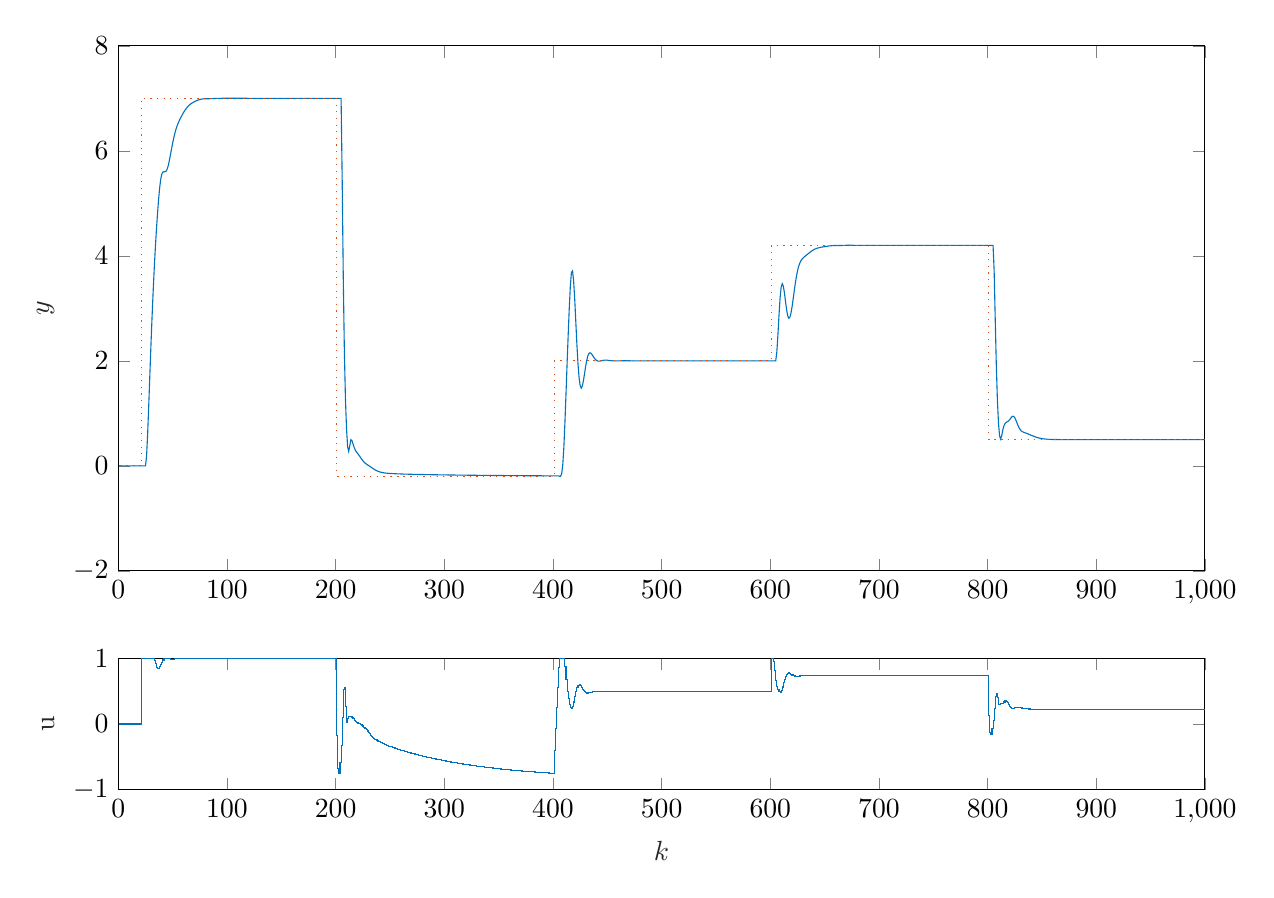
\begin{tikzpicture}

\begin{axis}[%
width=5.433in,
height=0.656in,
at={(0.854in,0.525in)},
scale only axis,
xmin=0,
xmax=1000,
xtick={0,100,200,300,400,500,600,700,800,900,1000},
xlabel style={font=\color{white!15!black}},
xlabel={$k$},
ymin=-1,
ymax=1,
ytick={-1,0,1},
ylabel style={font=\color{white!15!black}},
ylabel={u},
axis background/.style={fill=white}
]
\addplot[const plot, color=mycolor1, forget plot] table[row sep=crcr] {%
1	0\\
2	0\\
3	0\\
4	0\\
5	0\\
6	0\\
7	0\\
8	0\\
9	0\\
10	0\\
11	0\\
12	0\\
13	0\\
14	0\\
15	0\\
16	0\\
17	0\\
18	0\\
19	0\\
20	0\\
21	1\\
22	1\\
23	1\\
24	1\\
25	1\\
26	1\\
27	1\\
28	1\\
29	1\\
30	1\\
31	1\\
32	1\\
33	0.969645680797485\\
34	0.915877890890363\\
35	0.86817608582415\\
36	0.845028153787442\\
37	0.849420887458034\\
38	0.873908082496212\\
39	0.908350547224407\\
40	0.944283661451007\\
41	0.9760202417235\\
42	1\\
43	1\\
44	1\\
45	1\\
46	0.997992195032144\\
47	0.993734120241275\\
48	0.989721541099648\\
49	0.987774160448515\\
50	0.988231662540169\\
51	0.990430397433041\\
52	0.993438245802131\\
53	0.996471088119038\\
54	0.999020229967212\\
55	1\\
56	1\\
57	1\\
58	0.999870861303671\\
59	0.999426102743709\\
60	0.998906748581929\\
61	0.998556549104501\\
62	0.998511078841381\\
63	0.998778147413843\\
64	0.999291630540043\\
65	0.999948486734581\\
66	1\\
67	1\\
68	1\\
69	1\\
70	0.999886067574619\\
71	0.999700865707907\\
72	0.999060763645131\\
73	0.998184457059634\\
74	0.997402048204694\\
75	0.996936986033732\\
76	0.996857622897316\\
77	0.997095591910319\\
78	0.997501520562857\\
79	0.997913150139259\\
80	0.998213975498365\\
81	0.998360869828417\\
82	0.998377451896041\\
83	0.99832472788346\\
84	0.998266324016426\\
85	0.998243079215634\\
86	0.99826416765141\\
87	0.9983134958281\\
88	0.998364434323959\\
89	0.998393712903763\\
90	0.99838893207219\\
91	0.998349609272291\\
92	0.998284294612914\\
93	0.998206252769296\\
94	0.998129296469916\\
95	0.998064632961916\\
96	0.998019127583579\\
97	0.997994975223438\\
98	0.99799042987143\\
99	0.99800067760492\\
100	0.998019236966295\\
101	0.998039742682895\\
102	0.998057365149402\\
103	0.998069429493485\\
104	0.998075304984472\\
105	0.99807586316327\\
106	0.998072795366335\\
107	0.998067990719847\\
108	0.99806308260522\\
109	0.99805919649182\\
110	0.998056879304002\\
111	0.998056137118879\\
112	0.998056556103801\\
113	0.998057504275221\\
114	0.998058350038866\\
115	0.998058623575195\\
116	0.998058099841978\\
117	0.998056816735556\\
118	0.998055043740402\\
119	0.998053196737274\\
120	0.99805169864592\\
121	0.998050849000357\\
122	0.998050733668194\\
123	0.998051454676491\\
124	0.998052977094682\\
125	0.998055044181874\\
126	0.998057238924572\\
127	0.998059123309058\\
128	0.998060374041011\\
129	0.998060861876939\\
130	0.998060656810695\\
131	0.998059970258155\\
132	0.998059065889722\\
133	0.998058175570152\\
134	0.998057446966729\\
135	0.998056931946603\\
136	0.998056608330249\\
137	0.998056417850405\\
138	0.998056302190796\\
139	0.998056224902877\\
140	0.998056176209764\\
141	0.998056165241639\\
142	0.998056207153342\\
143	0.998056311521911\\
144	0.99805647563341\\
145	0.998056683514855\\
146	0.998056909610499\\
147	0.998057124975973\\
148	0.998057303709377\\
149	0.998057427852277\\
150	0.998057490031961\\
151	0.998057493637911\\
152	0.99805745073325\\
153	0.998057378440923\\
154	0.998057294889887\\
155	0.998057215743724\\
156	0.998057151964911\\
157	0.998057109012465\\
158	0.998057087293416\\
159	0.998057083461134\\
160	0.998057092081861\\
161	0.998057107243674\\
162	0.998057123821322\\
163	0.998057138251974\\
164	0.998057148787879\\
165	0.99805715529675\\
166	0.998057158764885\\
167	0.998057160686471\\
168	0.998057162496048\\
169	0.998057165149219\\
170	0.998057168913197\\
171	0.998057173394434\\
172	0.99805717776487\\
173	0.998057181098088\\
174	0.998057182589043\\
175	0.998057181730098\\
176	0.998057178450855\\
177	0.998057173167642\\
178	0.998057166703987\\
179	0.998057160097532\\
180	0.998057154354731\\
181	0.998057150230257\\
182	0.998057148093168\\
183	0.998057147906869\\
184	0.998057149310622\\
185	0.998057151761624\\
186	0.998057154686667\\
187	0.998057157600817\\
188	0.998057160170601\\
189	0.998057162221572\\
190	0.99805716370667\\
191	0.998057164658285\\
192	0.998057165143945\\
193	0.998057165236975\\
194	0.998057165004418\\
195	0.998057164507911\\
196	0.998057163810446\\
197	0.998057162982395\\
198	0.998057162102667\\
199	0.998057161253982\\
200	0.998057160513851\\
201	-0.180870167949454\\
202	-0.683902763524147\\
203	-0.754187203481092\\
204	-0.589314652124831\\
205	-0.332945675905062\\
206	0.102557777737974\\
207	0.530200193555079\\
208	0.557453584628887\\
209	0.260829601297582\\
210	0.0309495794879292\\
211	0.0837358566437056\\
212	0.110597770269055\\
213	0.108399873361722\\
214	0.114177341089862\\
215	0.106092433994175\\
216	0.0789936506667328\\
217	0.0564392952605091\\
218	0.0390016563329589\\
219	0.0259243271407814\\
220	0.0159639404801106\\
221	0.00813034335974763\\
222	0.00173064015238415\\
223	-0.00443956628975705\\
224	-0.0156416917409537\\
225	-0.0304464420472107\\
226	-0.0476606618290791\\
227	-0.0664571939716882\\
228	-0.0863261587251599\\
229	-0.106949513319615\\
230	-0.128065028237568\\
231	-0.148950638429041\\
232	-0.168395352721147\\
233	-0.186269934066643\\
234	-0.202519455595694\\
235	-0.217170797147763\\
236	-0.230322952855837\\
237	-0.242132142606306\\
238	-0.252791895326059\\
239	-0.262504844666938\\
240	-0.271460641944845\\
241	-0.279823071958864\\
242	-0.287725040622901\\
243	-0.295268965855042\\
244	-0.302530338475244\\
245	-0.30956271661831\\
246	-0.316402941285491\\
247	-0.323075839416497\\
248	-0.329598079056003\\
249	-0.335981099608757\\
250	-0.342233190940069\\
251	-0.348360869499529\\
252	-0.354369720732234\\
253	-0.360264865368525\\
254	-0.366051180511721\\
255	-0.371733375212352\\
256	-0.377315990496436\\
257	-0.382803368928671\\
258	-0.38819961985916\\
259	-0.393508593281179\\
260	-0.398733866808802\\
261	-0.403878745431717\\
262	-0.408946271383743\\
263	-0.413939240799199\\
264	-0.418860224073777\\
265	-0.423711587490379\\
266	-0.428495514407623\\
267	-0.433214024974047\\
268	-0.437868993853575\\
269	-0.442462165817637\\
270	-0.446995169292939\\
271	-0.451469528074041\\
272	-0.455886671454704\\
273	-0.460247943030912\\
274	-0.464554608402766\\
275	-0.468807861966655\\
276	-0.473008832952242\\
277	-0.477158590825763\\
278	-0.481258150153945\\
279	-0.485308475001747\\
280	-0.489310482921418\\
281	-0.493265048579029\\
282	-0.497173007056564\\
283	-0.501035156861878\\
284	-0.504852262674629\\
285	-0.508625057853081\\
286	-0.512354246724101\\
287	-0.516040506676517\\
288	-0.519684490076047\\
289	-0.523286826018342\\
290	-0.526848121935049\\
291	-0.530368965066381\\
292	-0.533849923812363\\
293	-0.537291548973705\\
294	-0.540694374892172\\
295	-0.544058920499362\\
296	-0.547385690281913\\
297	-0.550675175170385\\
298	-0.55392785335838\\
299	-0.557144191057823\\
300	-0.560324643195793\\
301	-0.563469654057784\\
302	-0.56657965788185\\
303	-0.569655079407658\\
304	-0.572696334384158\\
305	-0.575703830039218\\
306	-0.578677965514296\\
307	-0.581619132266969\\
308	-0.584527714443875\\
309	-0.587404089226416\\
310	-0.59024862715139\\
311	-0.593061692408519\\
312	-0.595843643116681\\
313	-0.598594831580513\\
314	-0.601315604528916\\
315	-0.604006303336848\\
316	-0.606667264231727\\
317	-0.60929881848559\\
318	-0.611901292594134\\
319	-0.61447500844363\\
320	-0.617020283466631\\
321	-0.619537430787335\\
322	-0.622026759357391\\
323	-0.624488574082862\\
324	-0.626923175943023\\
325	-0.629330862101605\\
326	-0.63171192601106\\
327	-0.634066657510363\\
328	-0.636395342916844\\
329	-0.638698265112491\\
330	-0.64097570362514\\
331	-0.643227934704938\\
332	-0.645455231396425\\
333	-0.647657863606556\\
334	-0.649836098168983\\
335	-0.651990198904855\\
336	-0.654120426680402\\
337	-0.656227039461539\\
338	-0.658310292365714\\
339	-0.660370437711193\\
340	-0.662407725063982\\
341	-0.664422401282545\\
342	-0.666414710560496\\
343	-0.668384894467394\\
344	-0.670333191987794\\
345	-0.672259839558672\\
346	-0.674165071105342\\
347	-0.676049118075978\\
348	-0.677912209474831\\
349	-0.679754571894248\\
350	-0.681576429545566\\
351	-0.68337800428896\\
352	-0.685159515662334\\
353	-0.686921180909298\\
354	-0.688663215006313\\
355	-0.690385830689056\\
356	-0.692089238478049\\
357	-0.693773646703616\\
358	-0.695439261530205\\
359	-0.697086286980111\\
360	-0.698714924956656\\
361	-0.700325375266844\\
362	-0.701917835643532\\
363	-0.703492501767147\\
364	-0.705049567286977\\
365	-0.706589223842063\\
366	-0.708111661081708\\
367	-0.709617066685635\\
368	-0.711105626383812\\
369	-0.712577523975957\\
370	-0.714032941350743\\
371	-0.715472058504728\\
372	-0.716895053561006\\
373	-0.718302102787606\\
374	-0.719693380615654\\
375	-0.721069059657296\\
376	-0.722429310723402\\
377	-0.723774302841062\\
378	-0.725104203270873\\
379	-0.72641917752404\\
380	-0.727719389379278\\
381	-0.72900500089955\\
382	-0.730276172448613\\
383	-0.731533062707413\\
384	-0.732775828690305\\
385	-0.734004625761117\\
386	-0.735219607649073\\
387	-0.736420926464546\\
388	-0.737608732714685\\
389	-0.738783175318888\\
390	-0.739944401624139\\
391	-0.741092557420216\\
392	-0.742227786954757\\
393	-0.743350232948197\\
394	-0.744460036608585\\
395	-0.745557337646261\\
396	-0.746642274288425\\
397	-0.747714983293568\\
398	-0.748775599965795\\
399	-0.749824258169019\\
400	-0.750861090341047\\
401	-0.405646499286119\\
402	-0.0724214675250411\\
403	0.249061248447714\\
404	0.559111789212175\\
405	0.858073118271085\\
406	1\\
407	1\\
408	1\\
409	1\\
410	1\\
411	0.874045296851037\\
412	0.680356171701545\\
413	0.496862827529508\\
414	0.384353881631164\\
415	0.303346038736115\\
416	0.253597053559648\\
417	0.242081469026675\\
418	0.27216824581186\\
419	0.335960998890326\\
420	0.417047311151947\\
421	0.494436724398919\\
422	0.552667438458968\\
423	0.58807546452738\\
424	0.597828942761432\\
425	0.58591964124699\\
426	0.56114828401541\\
427	0.533043495947538\\
428	0.508352762898525\\
429	0.490093026359429\\
430	0.478616252398684\\
431	0.473058791549246\\
432	0.472263613291475\\
433	0.474944442647201\\
434	0.479657974366368\\
435	0.485066549472777\\
436	0.490052796744214\\
437	0.493829496914282\\
438	0.496021473336821\\
439	0.496689455501633\\
440	0.496191772103277\\
441	0.495002838324339\\
442	0.493396351177685\\
443	0.491801369577231\\
444	0.490538026384585\\
445	0.489743958457029\\
446	0.489404439854545\\
447	0.489405993722649\\
448	0.489599696022995\\
449	0.489861390974054\\
450	0.490122916307069\\
451	0.490368973532773\\
452	0.490610443187885\\
453	0.490853134658675\\
454	0.491082682153069\\
455	0.491270619370728\\
456	0.491391755516445\\
457	0.491436164473571\\
458	0.49140942754153\\
459	0.491326078307896\\
460	0.491204956610738\\
461	0.491066231217236\\
462	0.490929503509952\\
463	0.490812596411342\\
464	0.490729791984848\\
465	0.490689326293869\\
466	0.490691554242833\\
467	0.490729065923538\\
468	0.490788936368923\\
469	0.49085635732823\\
470	0.490918213967283\\
471	0.490965419926766\\
472	0.490993667566862\\
473	0.491002941602547\\
474	0.490996377294297\\
475	0.490978929643194\\
476	0.490956122563075\\
477	0.490933022642566\\
478	0.490913525043141\\
479	0.490899985052176\\
480	0.490893174553463\\
481	0.490892519186338\\
482	0.490896525963949\\
483	0.49090332759728\\
484	0.490911068297036\\
485	0.490918203949012\\
486	0.490923693360789\\
487	0.490927057469758\\
488	0.490928319442502\\
489	0.490927865071791\\
490	0.490926269435287\\
491	0.490924133602495\\
492	0.490921963699442\\
493	0.490920107463351\\
494	0.490918745594\\
495	0.490917920817824\\
496	0.490917582476427\\
497	0.490917628942259\\
498	0.490917940072625\\
499	0.490918399444698\\
500	0.490918908374547\\
501	0.490919392696762\\
502	0.490919803664749\\
503	0.490920114920273\\
504	0.490920317532849\\
505	0.490920414919442\\
506	0.490920418892937\\
507	0.490920347108959\\
508	0.490920221344264\\
509	0.490920065781242\\
510	0.490919904757372\\
511	0.490919760044216\\
512	0.490919648232388\\
513	0.490919578920136\\
514	0.490919554153711\\
515	0.490919569169218\\
516	0.49091961415351\\
517	0.490919676568048\\
518	0.490919743550418\\
519	0.490919803976192\\
520	0.490919849892929\\
521	0.490919877195185\\
522	0.49091988555454\\
523	0.490919877739157\\
524	0.490919858529239\\
525	0.490919833512793\\
526	0.490919807996382\\
527	0.490919786189891\\
528	0.49091977074667\\
529	0.490919762665793\\
530	0.490919761498713\\
531	0.49091976575972\\
532	0.490919773423201\\
533	0.49091978239925\\
534	0.490919790906421\\
535	0.490919797697694\\
536	0.490919802134045\\
537	0.490919804131271\\
538	0.490919804024077\\
539	0.490919802395348\\
540	0.490919799911008\\
541	0.490919797187696\\
542	0.4909197947066\\
543	0.490919792774838\\
544	0.490919791527064\\
545	0.490919790955075\\
546	0.490919790951875\\
547	0.490919791358161\\
548	0.490919792002468\\
549	0.490919792730205\\
550	0.490919793420483\\
551	0.49091979399228\\
552	0.490919794402876\\
553	0.490919794641676\\
554	0.490919794722063\\
555	0.490919794673055\\
556	0.490919794531825\\
557	0.490919794337534\\
558	0.490919794126604\\
559	0.490919793929384\\
560	0.490919793768103\\
561	0.490919793656005\\
562	0.490919793597534\\
563	0.490919793589411\\
564	0.490919793622421\\
565	0.490919793683631\\
566	0.490919793758748\\
567	0.490919793834299\\
568	0.490919793899364\\
569	0.490919793946664\\
570	0.490919793972957\\
571	0.490919793978759\\
572	0.490919793967555\\
573	0.490919793944689\\
574	0.490919793916169\\
575	0.490919793887601\\
576	0.490919793863385\\
577	0.490919793846277\\
578	0.490919793837302\\
579	0.490919793835972\\
580	0.490919793840704\\
581	0.490919793849324\\
582	0.49091979385956\\
583	0.490919793869426\\
584	0.490919793877476\\
585	0.49091979388291\\
586	0.490919793885538\\
587	0.49091979388566\\
588	0.490919793883895\\
589	0.490919793880998\\
590	0.490919793877704\\
591	0.490919793874617\\
592	0.490919793872149\\
593	0.490919793870508\\
594	0.490919793869719\\
595	0.490919793869674\\
596	0.490919793870182\\
597	0.490919793871022\\
598	0.490919793871985\\
599	0.490919793872902\\
600	0.490919793873656\\
601	1\\
602	1\\
603	0.951501444987074\\
604	0.811118508259427\\
605	0.667533972311978\\
606	0.574395687155647\\
607	0.527817736577517\\
608	0.489369417926077\\
609	0.484285641658441\\
610	0.512476147997102\\
611	0.56488618402135\\
612	0.626604655877468\\
613	0.68488567169429\\
614	0.731157525157593\\
615	0.761086788813131\\
616	0.775149036108216\\
617	0.777482974449341\\
618	0.770291236909953\\
619	0.758599753877971\\
620	0.747020224789194\\
621	0.73770595504094\\
622	0.731393415752352\\
623	0.727965351906397\\
624	0.72694746916004\\
625	0.727722168378573\\
626	0.729641031937052\\
627	0.732108363746859\\
628	0.734638797076541\\
629	0.736888395512991\\
630	0.73865993518786\\
631	0.739886645507731\\
632	0.740601624028018\\
633	0.740901300354218\\
634	0.74091047787153\\
635	0.740754219849986\\
636	0.74053908939569\\
637	0.74034380570226\\
638	0.740217690127479\\
639	0.74018442760199\\
640	0.740248510256644\\
641	0.74040203292198\\
642	0.740630081721541\\
643	0.740913686912022\\
644	0.741230169516772\\
645	0.741551726178912\\
646	0.741844331762901\\
647	0.742070585768501\\
648	0.742202125060223\\
649	0.742236057202696\\
650	0.742193120072945\\
651	0.742108012401089\\
652	0.741855061026796\\
653	0.741511547102906\\
654	0.741203320583064\\
655	0.741024743196788\\
656	0.741011640769767\\
657	0.74115085144718\\
658	0.741395046734541\\
659	0.741679808484214\\
660	0.741940957681792\\
661	0.742127768804266\\
662	0.742211925105502\\
663	0.742191144060187\\
664	0.742085136770799\\
665	0.741927072175548\\
666	0.741754065720475\\
667	0.741598873667285\\
668	0.741484210697606\\
669	0.741420420618817\\
670	0.741406306293551\\
671	0.741432159731937\\
672	0.741483745515382\\
673	0.741546134852755\\
674	0.741606559185232\\
675	0.741655988770219\\
676	0.741689586718337\\
677	0.74170633461994\\
678	0.741708145268422\\
679	0.741698754234693\\
680	0.741682629437698\\
681	0.741664067005877\\
682	0.741646565199135\\
683	0.741632498345062\\
684	0.741623058619187\\
685	0.741618399501422\\
686	0.741617900961491\\
687	0.741620479610183\\
688	0.741624881966065\\
689	0.741629919812743\\
690	0.741634628124375\\
691	0.741638344329138\\
692	0.741640720561563\\
693	0.74164168748307\\
694	0.741641390022539\\
695	0.74164011356691\\
696	0.741638215141761\\
697	0.741636068318646\\
698	0.741634022670154\\
699	0.741632368836183\\
700	0.741631301426478\\
701	0.741630893487822\\
702	0.741631094010115\\
703	0.741631824309093\\
704	0.741632945560907\\
705	0.741634243307539\\
706	0.741635460715096\\
707	0.741636360732789\\
708	0.741636782565418\\
709	0.741636674126756\\
710	0.741636095223776\\
711	0.741635194715825\\
712	0.741634170807462\\
713	0.741633225310466\\
714	0.741632522134682\\
715	0.741632158920144\\
716	0.741632156502294\\
717	0.741632465812873\\
718	0.74163298792051\\
719	0.741633600825082\\
720	0.741634186292733\\
721	0.741634651210415\\
722	0.741634940144482\\
723	0.741635038299536\\
724	0.741634966230262\\
725	0.741634769088259\\
726	0.741634503678367\\
727	0.741634226246789\\
728	0.741633983065651\\
729	0.741633804852489\\
730	0.741633705114003\\
731	0.74163368178239\\
732	0.741633721087185\\
733	0.741633802473736\\
734	0.741633903488906\\
735	0.741634003824286\\
736	0.741634088049035\\
737	0.741634146900611\\
738	0.741634177275265\\
739	0.741634181240194\\
740	0.74163416446902\\
741	0.741634134494179\\
742	0.741634099098491\\
743	0.741634065062606\\
744	0.74163403737241\\
745	0.741634018891511\\
746	0.741634010430826\\
747	0.74163401110392\\
748	0.741634018841822\\
749	0.741634030951086\\
750	0.741634044629237\\
751	0.741634057388624\\
752	0.741634067360628\\
753	0.741634073464366\\
754	0.741634075403171\\
755	0.741634073558478\\
756	0.741634068829347\\
757	0.741634062436453\\
758	0.741634055703336\\
759	0.741634049839211\\
760	0.741634045755762\\
761	0.741634043947651\\
762	0.741634044454713\\
763	0.741634046907067\\
764	0.741634050638158\\
765	0.741634054838814\\
766	0.741634058719572\\
767	0.741634061649809\\
768	0.741634063250042\\
769	0.741634063425792\\
770	0.741634062344373\\
771	0.741634060366994\\
772	0.741634057955538\\
773	0.741634055575395\\
774	0.741634053613149\\
775	0.741634052321998\\
776	0.741634051800258\\
777	0.741634052001114\\
778	0.7416340527662\\
779	0.741634053872555\\
780	0.741634055082066\\
781	0.741634056184165\\
782	0.741634057025612\\
783	0.741634057524744\\
784	0.741634057670849\\
785	0.741634057511791\\
786	0.741634057134407\\
787	0.741634056642492\\
788	0.741634056136571\\
789	0.741634055698438\\
790	0.741634055382019\\
791	0.741634055210686\\
792	0.741634055180055\\
793	0.74163405526463\\
794	0.741634055426358\\
795	0.74163405562331\\
796	0.741634055817082\\
797	0.74163405597802\\
798	0.741634056087948\\
799	0.741634056140519\\
800	0.741634056139673\\
801	0.135796401484858\\
802	-0.122706460013206\\
803	-0.158824852773257\\
804	-0.0740986806491621\\
805	0.0576464875218904\\
806	0.232231609760676\\
807	0.421069019443233\\
808	0.463897116858931\\
809	0.400217201269166\\
810	0.301038439034704\\
811	0.295427812877598\\
812	0.306661255629517\\
813	0.309361498078003\\
814	0.317509388931288\\
815	0.336341090734892\\
816	0.350600931186506\\
817	0.34623282255239\\
818	0.32390778934084\\
819	0.294399627485014\\
820	0.267819098794392\\
821	0.249499192459742\\
822	0.240327995735311\\
823	0.238663288856996\\
824	0.241855316743659\\
825	0.247036730125177\\
826	0.251656027759209\\
827	0.25384078906038\\
828	0.252916989599438\\
829	0.250234897568788\\
830	0.246940868492938\\
831	0.243691013592701\\
832	0.240776106650982\\
833	0.23830056678715\\
834	0.236220957724962\\
835	0.234383812734564\\
836	0.232630639377408\\
837	0.230895601640198\\
838	0.229219430052284\\
839	0.22769033397224\\
840	0.226386627901291\\
841	0.225340918244279\\
842	0.224635271184345\\
843	0.224151547057971\\
844	0.223761157754994\\
845	0.223393102155417\\
846	0.223034483886961\\
847	0.222705174546699\\
848	0.222432799604654\\
849	0.222236104470861\\
850	0.222114058461199\\
851	0.222046811351093\\
852	0.222006559223115\\
853	0.221970437677197\\
854	0.221928122912509\\
855	0.221881641067634\\
856	0.221839614262744\\
857	0.221810715829442\\
858	0.221798930704686\\
859	0.221801985989968\\
860	0.221813165264746\\
861	0.221824989859043\\
862	0.221832515616329\\
863	0.221834694013452\\
864	0.221833590901017\\
865	0.221832379245487\\
866	0.221833394635268\\
867	0.22183716624656\\
868	0.221842613965406\\
869	0.221847990415689\\
870	0.221851904527968\\
871	0.221853903591331\\
872	0.221854445810835\\
873	0.221854437505925\\
874	0.221854676614017\\
875	0.221855504471496\\
876	0.221856780647793\\
877	0.221858101060654\\
878	0.221859082213674\\
879	0.221859554342326\\
880	0.221859596414103\\
881	0.221859437907541\\
882	0.221859311985795\\
883	0.221859331500485\\
884	0.221859482183538\\
885	0.221859676234122\\
886	0.221859821347015\\
887	0.221859870239445\\
888	0.221859832387254\\
889	0.221859753021642\\
890	0.221859679899469\\
891	0.221859639315524\\
892	0.221859631063074\\
893	0.221859638686769\\
894	0.221859644419202\\
895	0.221859639275333\\
896	0.221859624624514\\
897	0.221859607438854\\
898	0.221859594007511\\
899	0.221859586248478\\
900	0.22185958200635\\
901	0.221859577894029\\
902	0.221859572092419\\
903	0.22185956529919\\
904	0.221859559684562\\
905	0.221859557020347\\
906	0.221859557401425\\
907	0.221859559286838\\
908	0.221859560601888\\
909	0.221859560030169\\
910	0.22185955766932\\
911	0.22185955475707\\
912	0.221859552778076\\
913	0.221859552569643\\
914	0.22185955393694\\
915	0.22185955590856\\
916	0.221859557378746\\
917	0.221859557713181\\
918	0.221859556994532\\
919	0.221859555842307\\
920	0.221859554983988\\
921	0.221859554852244\\
922	0.221859555415561\\
923	0.22185955628512\\
924	0.221859556990505\\
925	0.221859557239728\\
926	0.22185955703099\\
927	0.221859556591105\\
928	0.22185955621008\\
929	0.221859556079822\\
930	0.221859556219096\\
931	0.22185955650396\\
932	0.221859556764002\\
933	0.221859556879824\\
934	0.221859556831606\\
935	0.221859556685517\\
936	0.221859556539746\\
937	0.2218595564674\\
938	0.221859556486067\\
939	0.221859556562979\\
940	0.221859556644343\\
941	0.221859556687896\\
942	0.221859556681312\\
943	0.221859556640699\\
944	0.221859556595054\\
945	0.221859556568223\\
946	0.221859556568218\\
947	0.221859556587402\\
948	0.221859556610576\\
949	0.221859556624749\\
950	0.22185955662513\\
951	0.2218595566153\\
952	0.221859556603056\\
953	0.221859556595239\\
954	0.221859556594495\\
955	0.2218595565991\\
956	0.221859556605091\\
957	0.221859556608953\\
958	0.221859556609313\\
959	0.221859556607031\\
960	0.221859556604095\\
961	0.221859556602246\\
962	0.221859556602129\\
963	0.221859556603272\\
964	0.221859556604672\\
965	0.221859556605488\\
966	0.221859556605453\\
967	0.22185955660485\\
968	0.221859556604194\\
969	0.221859556603875\\
970	0.221859556603978\\
971	0.221859556604322\\
972	0.221859556604634\\
973	0.221859556604736\\
974	0.221859556604621\\
975	0.221859556604413\\
976	0.22185955660426\\
977	0.221859556604242\\
978	0.221859556604342\\
979	0.221859556604475\\
980	0.221859556604555\\
981	0.221859556604546\\
982	0.221859556604471\\
983	0.221859556604386\\
984	0.221859556604342\\
985	0.221859556604356\\
986	0.221859556604409\\
987	0.221859556604464\\
988	0.221859556604491\\
989	0.22185955660448\\
990	0.221859556604446\\
991	0.221859556604411\\
992	0.221859556604394\\
993	0.221859556604401\\
994	0.221859556604423\\
995	0.221859556604445\\
996	0.221859556604455\\
997	0.221859556604451\\
998	0.221859556604438\\
999	0.221859556604425\\
1000	0.221859556604418\\
};
\end{axis}

\begin{axis}[%
width=5.433in,
height=2.625in,
at={(0.854in,1.619in)},
scale only axis,
xmin=0,
xmax=1000,
xtick={0,100,200,300,400,500,600,700,800,900,1000},
ymin=-2,
ymax=8,
ytick={-2,0,2,4,6,8},
ylabel style={font=\color{white!15!black}},
ylabel={$y$},
axis background/.style={fill=white}
]
\addplot [color=mycolor1, forget plot]
  table[row sep=crcr]{%
1	0\\
2	0\\
3	0\\
4	0\\
5	0\\
6	0\\
7	0\\
8	0\\
9	0\\
10	0\\
11	0\\
12	0\\
13	0\\
14	0\\
15	0\\
16	0\\
17	0\\
18	0\\
19	0\\
20	0\\
21	0\\
22	0\\
23	0\\
24	0\\
25	0\\
26	0.187021166666667\\
27	0.6177121086775\\
28	1.15713812513778\\
29	1.72826134563714\\
30	2.28857090407221\\
31	2.81598000810106\\
32	3.30033523448568\\
33	3.73832226743667\\
34	4.13042497668062\\
35	4.47912397208548\\
36	4.78784169917674\\
37	5.06033571970525\\
38	5.28888100455265\\
39	5.45675291681498\\
40	5.55570036678074\\
41	5.59586271996783\\
42	5.60152517470199\\
43	5.60004372722649\\
44	5.61298350799135\\
45	5.6526220793015\\
46	5.7223742943795\\
47	5.81881062030471\\
48	5.92844217458697\\
49	6.03978001467634\\
50	6.14663070742613\\
51	6.24512107595084\\
52	6.33237538736467\\
53	6.40714004296269\\
54	6.4702162916757\\
55	6.52389235850498\\
56	6.57092380028626\\
57	6.61369881915482\\
58	6.65383083284735\\
59	6.69211519416196\\
60	6.72835210893742\\
61	6.76189438315579\\
62	6.79237819247011\\
63	6.81970511154983\\
64	6.8438257466211\\
65	6.86478946376389\\
66	6.88283346191832\\
67	6.89837718777456\\
68	6.91194105788279\\
69	6.92404794026147\\
70	6.93514388018699\\
71	6.94528648533467\\
72	6.95443848100666\\
73	6.96262014496273\\
74	6.96988927837765\\
75	6.9762735297526\\
76	6.98178337068492\\
77	6.98626661917869\\
78	6.9895237661088\\
79	6.99151069616006\\
80	6.99241202281299\\
81	6.99258799129271\\
82	6.99245674738417\\
83	6.99237411515481\\
84	6.99255498657228\\
85	6.99305554085643\\
86	6.99380907412424\\
87	6.99469001045709\\
88	6.99557656589673\\
89	6.99639071284149\\
90	6.99710823509811\\
91	6.99774479011351\\
92	6.9983311857059\\
93	6.99889123679423\\
94	6.99943011352777\\
95	6.99993409013126\\
96	7.00037795477462\\
97	7.00073509456434\\
98	7.00098627570366\\
99	7.00112490784005\\
100	7.00115823077939\\
101	7.00110506719108\\
102	7.00099145401886\\
103	7.00084561092814\\
104	7.00069327604149\\
105	7.00055418097159\\
106	7.00044026078099\\
107	7.00035573810928\\
108	7.00029867512235\\
109	7.0002632793781\\
110	7.00024225602474\\
111	7.00022870322077\\
112	7.00021730904874\\
113	7.00020483468483\\
114	7.00019002002029\\
115	7.00017311864942\\
116	7.00015526318713\\
117	7.00013782730082\\
118	7.000121919526\\
119	7.00010809367684\\
120	7.00009628920623\\
121	7.00008595605012\\
122	7.00007629180737\\
123	7.00006651687704\\
124	7.00005611614252\\
125	7.00004498003409\\
126	7.0000334095514\\
127	7.00002199110116\\
128	7.0000114900824\\
129	7.00000273103391\\
130	6.99999641763989\\
131	6.99999294211855\\
132	6.99999226565918\\
133	6.99999392032044\\
134	6.99999712927206\\
135	7.00000099845447\\
136	7.00000471363162\\
137	7.00000768474932\\
138	7.00000960658777\\
139	7.00001043725117\\
140	7.00001032114512\\
141	7.00000949345303\\
142	7.00000819855367\\
143	7.00000664063965\\
144	7.00000496850806\\
145	7.00000328462097\\
146	7.00000166413475\\
147	7.0000001717512\\
148	6.99999886978559\\
149	6.99999781659816\\
150	6.99999705854499\\
151	6.99999662025613\\
152	6.99999649763946\\
153	6.99999665630161\\
154	6.9999970359534\\
155	6.99999755963577\\
156	6.99999814554011\\
157	6.99999871879187\\
158	6.9999992208176\\
159	6.99999961472992\\
160	6.99999988626648\\
161	7.00000004085556\\
162	7.00000009808745\\
163	7.00000008513952\\
164	7.00000003057379\\
165	6.99999995952677\\
166	6.99999989079851\\
167	6.99999983586644\\
168	6.99999979948754\\
169	6.99999978134012\\
170	6.99999977809433\\
171	6.99999978537274\\
172	6.99999979922675\\
173	6.99999981695388\\
174	6.99999983726335\\
175	6.99999985993547\\
176	6.9999998852078\\
177	6.9999999131443\\
178	6.99999994320067\\
179	6.99999997405826\\
180	7.00000000371571\\
181	7.00000002979861\\
182	7.00000005001196\\
183	7.00000006262122\\
184	7.00000006683243\\
185	7.00000006296866\\
186	7.00000005239991\\
187	7.00000003725589\\
188	7.00000002000829\\
189	7.0000000030349\\
190	6.99999998826682\\
191	6.99999997698199\\
192	6.99999996975912\\
193	6.99999996656383\\
194	6.99999996691354\\
195	6.99999997006446\\
196	6.99999997517618\\
197	6.99999998143083\\
198	6.99999998810305\\
199	6.99999999459105\\
200	7.00000000042388\\
201	7.00000000525874\\
202	7.00000000887651\\
203	7.00000001117819\\
204	7.00000001217998\\
205	7.00000001200353\\
206	5.47605588485514\\
207	3.6050905640503\\
208	2.20372581600364\\
209	1.28533055329527\\
210	0.710156384143633\\
211	0.366280691631649\\
212	0.275913626284618\\
213	0.38430358520872\\
214	0.497332187628785\\
215	0.481701276846871\\
216	0.416390802538582\\
217	0.354344693413129\\
218	0.304828808541481\\
219	0.268375218572842\\
220	0.241014230093507\\
221	0.214526685986028\\
222	0.18530967012583\\
223	0.154502584986556\\
224	0.124462326238456\\
225	0.0970751947629167\\
226	0.0733161010579111\\
227	0.0533911796669497\\
228	0.0369378530060684\\
229	0.0227425158291985\\
230	0.00933430011135179\\
231	-0.00420590554381613\\
232	-0.0181656678267744\\
233	-0.0323972004234982\\
234	-0.0465481502026248\\
235	-0.0602297003488554\\
236	-0.0730946792706843\\
237	-0.0848513102729187\\
238	-0.0952886909230152\\
239	-0.104335806195952\\
240	-0.112037772208259\\
241	-0.11851296217638\\
242	-0.123915125915073\\
243	-0.128406957756083\\
244	-0.132144280344631\\
245	-0.135267580329138\\
246	-0.137898283860193\\
247	-0.14013799826937\\
248	-0.142069531604448\\
249	-0.143758884605533\\
250	-0.145257674650557\\
251	-0.146605638348249\\
252	-0.147832992194279\\
253	-0.148962525635566\\
254	-0.150011369883932\\
255	-0.150992433965155\\
256	-0.151915530416759\\
257	-0.152788230346272\\
258	-0.15361649464141\\
259	-0.15440512809204\\
260	-0.155158098805357\\
261	-0.155878758757429\\
262	-0.156569994171409\\
263	-0.157234327629167\\
264	-0.15787398794406\\
265	-0.158490959056947\\
266	-0.159087015563479\\
267	-0.159663749811022\\
268	-0.160222593640551\\
269	-0.160764836609911\\
270	-0.161291641752104\\
271	-0.161804059455263\\
272	-0.162303039790645\\
273	-0.162789443481876\\
274	-0.163264051648307\\
275	-0.163727574432617\\
276	-0.164180658616882\\
277	-0.164623894330215\\
278	-0.165057820949395\\
279	-0.165482932289607\\
280	-0.165899681175611\\
281	-0.166308483475088\\
282	-0.166709721666443\\
283	-0.167103748003909\\
284	-0.167490887333849\\
285	-0.167871439608129\\
286	-0.16824568213344\\
287	-0.168613871589506\\
288	-0.16897624584414\\
289	-0.169333025589\\
290	-0.1696844158165\\
291	-0.170030607155513\\
292	-0.170371777081196\\
293	-0.170708091012313\\
294	-0.17103970330776\\
295	-0.171366758172655\\
296	-0.171689390483099\\
297	-0.172007726537702\\
298	-0.172321884743074\\
299	-0.172631976239659\\
300	-0.172938105473628\\
301	-0.173240370719923\\
302	-0.173538864561006\\
303	-0.173833674325406\\
304	-0.174124882489712\\
305	-0.174412567047327\\
306	-0.174696801846926\\
307	-0.174977656903308\\
308	-0.175255198683044\\
309	-0.175529490367102\\
310	-0.17580059209243\\
311	-0.176068561174281\\
312	-0.176333452310903\\
313	-0.17659531777207\\
314	-0.1768542075728\\
315	-0.177110169633477\\
316	-0.177363249927489\\
317	-0.177613492617407\\
318	-0.177860940180615\\
319	-0.178105633525266\\
320	-0.178347612097308\\
321	-0.178586913979314\\
322	-0.178823575981757\\
323	-0.179057633727319\\
324	-0.179289121728798\\
325	-0.179518073461096\\
326	-0.179744521427766\\
327	-0.179968497222521\\
328	-0.18019003158612\\
329	-0.180409154458964\\
330	-0.180625895029748\\
331	-0.180840281780468\\
332	-0.181052342528059\\
333	-0.181262104462927\\
334	-0.181469594184604\\
335	-0.181674837734757\\
336	-0.181877860627744\\
337	-0.182078687878904\\
338	-0.182277344030754\\
339	-0.182473853177257\\
340	-0.182668238986295\\
341	-0.182860524720499\\
342	-0.183050733256544\\
343	-0.183238887103035\\
344	-0.183425008417093\\
345	-0.18360911901973\\
346	-0.183791240410107\\
347	-0.183971393778769\\
348	-0.184149600019923\\
349	-0.184325879742835\\
350	-0.184500253282414\\
351	-0.184672740709045\\
352	-0.18484336183773\\
353	-0.185012136236578\\
354	-0.185179083234709\\
355	-0.185344221929609\\
356	-0.185507571193977\\
357	-0.185669149682103\\
358	-0.185828975835818\\
359	-0.185987067890039\\
360	-0.186143443877954\\
361	-0.186298121635856\\
362	-0.186451118807676\\
363	-0.186602452849211\\
364	-0.186752141032102\\
365	-0.186900200447548\\
366	-0.187046648009807\\
367	-0.187191500459477\\
368	-0.18733477436659\\
369	-0.187476486133522\\
370	-0.187616651997745\\
371	-0.187755288034422\\
372	-0.187892410158865\\
373	-0.188028034128863\\
374	-0.188162175546897\\
375	-0.188294849862235\\
376	-0.188426072372938\\
377	-0.188555858227766\\
378	-0.188684222428006\\
379	-0.188811179829212\\
380	-0.188936745142884\\
381	-0.189060932938074\\
382	-0.189183757642932\\
383	-0.189305233546197\\
384	-0.189425374798639\\
385	-0.189544195414452\\
386	-0.189661709272597\\
387	-0.189777930118119\\
388	-0.189892871563417\\
389	-0.19000654708948\\
390	-0.190118970047101\\
391	-0.19023015365805\\
392	-0.190340111016235\\
393	-0.190448855088825\\
394	-0.19055639871736\\
395	-0.19066275461884\\
396	-0.19076793538679\\
397	-0.190871953492315\\
398	-0.19097482128513\\
399	-0.191076550994585\\
400	-0.191177154730671\\
401	-0.191276644485013\\
402	-0.191375032131852\\
403	-0.191472329429022\\
404	-0.191568548018905\\
405	-0.191663699429387\\
406	-0.198414710971834\\
407	-0.200592228298819\\
408	-0.15030295493181\\
409	0.0184285372953369\\
410	0.348520997203191\\
411	0.825732238874415\\
412	1.37982228114342\\
413	1.94795523849098\\
414	2.49602942935535\\
415	3.00687870861002\\
416	3.4300424058505\\
417	3.68578272233275\\
418	3.71264160599527\\
419	3.52417870042648\\
420	3.17706856717142\\
421	2.74816235809855\\
422	2.31796838041183\\
423	1.9507955893548\\
424	1.68368867648291\\
425	1.52886096358598\\
426	1.47996745359032\\
427	1.51792361369069\\
428	1.61707163632844\\
429	1.74879070123515\\
430	1.88508320700955\\
431	2.00306334019576\\
432	2.08858911786743\\
433	2.13728536166601\\
434	2.15270217473984\\
435	2.14297696059409\\
436	2.11766802565592\\
437	2.08563257985253\\
438	2.05390169445831\\
439	2.0272109624398\\
440	2.00801994851998\\
441	1.99683949702978\\
442	1.99272239088706\\
443	1.99382815552927\\
444	1.99799701292771\\
445	2.00323415046635\\
446	2.00802423770972\\
447	2.01138248343573\\
448	2.01287994433938\\
449	2.01259056527473\\
450	2.01093360502411\\
451	2.00847857631152\\
452	2.00577419219924\\
453	2.00323731600719\\
454	2.00111461532569\\
455	1.99950435910586\\
456	1.99840880820335\\
457	1.9977856629443\\
458	1.99757807928476\\
459	1.99772114613537\\
460	1.99813685103955\\
461	1.99873203828203\\
462	1.99940550193771\\
463	2.00006078382582\\
464	2.00061804321893\\
465	2.00102168832418\\
466	2.00124344178925\\
467	2.00128171364332\\
468	2.00115842911841\\
469	2.00091392632322\\
470	2.00059998023335\\
471	2.00027130991571\\
472	1.99997678885314\\
473	1.99975216036045\\
474	1.99961590869493\\
475	1.99956901792461\\
476	1.99959814131753\\
477	1.99968084000317\\
478	1.99979133117467\\
479	1.99990549390996\\
480	2.00000440534456\\
481	2.0000761707925\\
482	2.00011616841714\\
483	2.00012605216016\\
484	2.00011196639562\\
485	2.00008244096764\\
486	2.00004638529819\\
487	2.00001149919716\\
488	1.99998330026004\\
489	1.99996476724188\\
490	1.9999564935545\\
491	1.99995720186649\\
492	1.99996444796088\\
493	1.99997534624302\\
494	1.99998718272623\\
495	1.99999783296497\\
496	2.00000595900746\\
497	2.00001100896833\\
498	2.00001307620218\\
499	2.00001268800815\\
500	2.0000105871467\\
501	2.00000754953857\\
502	2.00000425783924\\
503	2.00000123171545\\
504	1.9999988051656\\
505	1.99999713765035\\
506	1.99999624575499\\
507	1.99999604381002\\
508	1.99999638463258\\
509	1.99999709468674\\
510	1.99999800097912\\
511	1.99999894947139\\
512	1.99999981630229\\
513	2.00000051354823\\
514	2.00000099090282\\
515	2.00000123403378\\
516	2.00000125996655\\
517	2.00000110987155\\
518	2.0000008399946\\
519	2.00000051187929\\
520	2.0000001832262\\
521	1.99999990061396\\
522	1.99999969492129\\
523	1.99999957976631\\
524	1.99999955275386\\
525	1.9999995988997\\
526	1.99999969534602\\
527	1.99999981641349\\
528	1.99999993813326\\
529	2.0000000416223\\
530	2.00000011497137\\
531	2.00000015362977\\
532	2.00000015952625\\
533	2.00000013932918\\
534	2.00000010231255\\
535	2.00000005826624\\
536	2.00000001579088\\
537	1.99999998117983\\
538	1.99999995794554\\
539	1.99999994692224\\
540	1.999999946791\\
541	1.99999995483414\\
542	1.99999996773199\\
543	1.99999998225426\\
544	1.99999999575554\\
545	2.00000000644308\\
546	2.00000001343334\\
547	2.0000000166458\\
548	2.00000001659674\\
549	2.00000001415523\\
550	2.00000001031193\\
551	2.00000000599474\\
552	2.00000000194738\\
553	1.99999999867157\\
554	1.99999999642263\\
555	1.99999999524287\\
556	1.99999999501581\\
557	1.99999999552669\\
558	1.99999999651858\\
559	1.99999999773769\\
560	1.99999999896538\\
561	2.00000000003671\\
562	2.00000000084746\\
563	2.00000000135202\\
564	2.00000000155493\\
565	2.00000000149863\\
566	2.00000000124958\\
567	2.0000000008847\\
568	2.00000000047934\\
569	2.00000000009802\\
570	1.99999999978818\\
571	1.99999999957746\\
572	1.99999999947394\\
573	1.999999999469\\
574	1.99999999954187\\
575	1.99999999966505\\
576	1.99999999980959\\
577	1.99999999994959\\
578	2.0000000000654\\
579	2.00000000014521\\
580	2.00000000018519\\
581	2.00000000018834\\
582	2.00000000016257\\
583	2.0000000001184\\
584	2.0000000000668\\
585	2.00000000001731\\
586	1.99999999997696\\
587	1.99999999994972\\
588	1.9999999999366\\
589	1.99999999993618\\
590	1.99999999994546\\
591	1.99999999996064\\
592	1.99999999997797\\
593	1.9999999999943\\
594	2.00000000000742\\
595	2.00000000001615\\
596	2.0000000000203\\
597	2.00000000002042\\
598	2.0000000000175\\
599	2.00000000001276\\
600	2.00000000000736\\
601	2.00000000000226\\
602	1.99999999999813\\
603	1.9999999999953\\
604	1.99999999999386\\
605	1.99999999999366\\
606	2.16535210394992\\
607	2.48866094042341\\
608	2.86541576456747\\
609	3.19563630026325\\
610	3.40328112209114\\
611	3.46950236980142\\
612	3.42255091845725\\
613	3.2954811624602\\
614	3.13084104465818\\
615	2.97412142565318\\
616	2.86108645774423\\
617	2.8112123244716\\
618	2.82842305484109\\
619	2.90493495113917\\
620	3.02549815371616\\
621	3.1716673269688\\
622	3.32583638064111\\
623	3.47302138775978\\
624	3.60250877939982\\
625	3.70894744005594\\
626	3.79170998882636\\
627	3.85336798536554\\
628	3.89812101150389\\
629	3.93057626240976\\
630	3.95495721908618\\
631	3.9746733302886\\
632	3.99216196102453\\
633	4.00892011762803\\
634	4.02565384149784\\
635	4.04248525445703\\
636	4.0591703012602\\
637	4.07529377594281\\
638	4.09042151635294\\
639	4.1042017216178\\
640	4.11641715277804\\
641	4.12699675218939\\
642	4.13599871628825\\
643	4.14357759860591\\
644	4.14994634538215\\
645	4.15534119266801\\
646	4.1599939513499\\
647	4.16411305940441\\
648	4.16787235219954\\
649	4.17140507292192\\
650	4.17480038719198\\
651	4.17810071234693\\
652	4.18130068019409\\
653	4.18435276166591\\
654	4.18718492215824\\
655	4.18972512560566\\
656	4.19192353429011\\
657	4.19369560098107\\
658	4.19495839485965\\
659	4.19570043294406\\
660	4.19600729781355\\
661	4.19603926225987\\
662	4.19598548374575\\
663	4.19601660585383\\
664	4.19624891717294\\
665	4.19672660200642\\
666	4.19742262894634\\
667	4.19825501257618\\
668	4.19911294933417\\
669	4.19988533751623\\
670	4.20048460729291\\
671	4.20086138319045\\
672	4.20100855890377\\
673	4.20095596728778\\
674	4.20075864053839\\
675	4.20048244949381\\
676	4.20019065816768\\
677	4.19993390837491\\
678	4.19974480997649\\
679	4.19963702777553\\
680	4.19960784904729\\
681	4.1996428289632\\
682	4.19972114419921\\
683	4.19982056215802\\
684	4.19992131247134\\
685	4.20000853104249\\
686	4.20007327220448\\
687	4.20011231751305\\
688	4.20012713998394\\
689	4.20012241852433\\
690	4.20010445962967\\
691	4.20007979882453\\
692	4.20005414970846\\
693	4.2000317665\\
694	4.20001520253179\\
695	4.20000539053447\\
696	4.20000194218735\\
697	4.20000356058469\\
698	4.20000847323426\\
699	4.20001481734556\\
700	4.20002093663162\\
701	4.20002557444091\\
702	4.20002796807386\\
703	4.20002786086159\\
704	4.20002544994186\\
705	4.2000212826426\\
706	4.20001611581087\\
707	4.200010759318\\
708	4.20000596174603\\
709	4.2000023248052\\
710	4.2000002260789\\
711	4.19999976263349\\
712	4.20000074046572\\
713	4.20000272185552\\
714	4.20000512227545\\
715	4.20000733345716\\
716	4.20000884342138\\
717	4.20000932741853\\
718	4.20000869290321\\
719	4.200007073428\\
720	4.20000477808849\\
721	4.20000221218386\\
722	4.19999978903811\\
723	4.19999785206364\\
724	4.19999662119766\\
725	4.19999617061398\\
726	4.19999643709624\\
727	4.19999725235927\\
728	4.19999838900547\\
729	4.19999960900753\\
730	4.20000070524708\\
731	4.20000152986228\\
732	4.20000200693532\\
733	4.20000213047135\\
734	4.20000195108744\\
735	4.20000155609903\\
736	4.20000104781437\\
737	4.20000052408108\\
738	4.20000006382715\\
739	4.19999971886402\\
740	4.19999951187362\\
741	4.19999943948807\\
742	4.19999947878482\\
743	4.19999959535594\\
744	4.1999997512933\\
745	4.19999991184321\\
746	4.20000004999952\\
747	4.20000014881007\\
748	4.20000020158771\\
749	4.20000021049819\\
750	4.20000018413237\\
751	4.20000013467633\\
752	4.20000007520223\\
753	4.20000001745429\\
754	4.1999999703368\\
755	4.19999993915843\\
756	4.19999992557073\\
757	4.19999992806326\\
758	4.19999994283555\\
759	4.19999996483649\\
760	4.19999998878337\\
761	4.20000001002617\\
762	4.20000002517297\\
763	4.20000003243205\\
764	4.20000003166142\\
765	4.20000002415296\\
766	4.20000001221315\\
767	4.19999999862911\\
768	4.19999998612028\\
769	4.19999997687015\\
770	4.19999997220982\\
771	4.19999997249154\\
772	4.19999997715171\\
773	4.19999998492894\\
774	4.1999999941775\\
775	4.20000000320711\\
776	4.20000001058366\\
777	4.20000001534194\\
778	4.20000001708467\\
779	4.20000001596722\\
780	4.20000001258813\\
781	4.20000000782017\\
782	4.20000000262138\\
783	4.19999999786276\\
784	4.19999999419985\\
785	4.1999999920028\\
786	4.1999999913465\\
787	4.19999999205145\\
788	4.19999999375919\\
789	4.19999999602286\\
790	4.19999999839503\\
791	4.20000000049864\\
792	4.20000000207259\\
793	4.20000000298978\\
794	4.20000000324993\\
795	4.20000000295376\\
796	4.20000000226642\\
797	4.2000000013783\\
798	4.20000000047009\\
799	4.19999999968676\\
800	4.1999999991226\\
801	4.19999999881743\\
802	4.1999999987621\\
803	4.19999999891046\\
804	4.19999999919444\\
805	4.19999999953942\\
806	3.71743180027523\\
807	2.79836102180449\\
808	1.91568579591466\\
809	1.25110837372487\\
810	0.811813685302822\\
811	0.571189537691048\\
812	0.509978219281416\\
813	0.576649797276513\\
814	0.686331949620556\\
815	0.763024648887839\\
816	0.802483269723752\\
817	0.824631193761454\\
818	0.839144695966758\\
819	0.852057251816997\\
820	0.870799007634081\\
821	0.897981921477645\\
822	0.926771042277942\\
823	0.944612352737456\\
824	0.941472167299081\\
825	0.915236971063195\\
826	0.87141075703737\\
827	0.819235498573953\\
828	0.767702839546338\\
829	0.723239437492096\\
830	0.689017415859129\\
831	0.665254543038326\\
832	0.649976059737911\\
833	0.640045834982321\\
834	0.6325418783295\\
835	0.62550988050589\\
836	0.617997466012505\\
837	0.609773282079353\\
838	0.601014101143669\\
839	0.592049292810744\\
840	0.583178652446653\\
841	0.57458328543248\\
842	0.566331328817908\\
843	0.558439223860567\\
844	0.550931634443619\\
845	0.543868095918867\\
846	0.537334223816921\\
847	0.531444891890197\\
848	0.526285009520713\\
849	0.52186158207363\\
850	0.518109805492331\\
851	0.514929299897841\\
852	0.512220858156998\\
853	0.509908229476602\\
854	0.507942835846984\\
855	0.506295350677792\\
856	0.504941724419197\\
857	0.503851986104872\\
858	0.502986804674432\\
859	0.502301606137591\\
860	0.50175424184748\\
861	0.501311457094932\\
862	0.500951386072558\\
863	0.500661828797897\\
864	0.500435896004144\\
865	0.500267424394265\\
866	0.500148184435366\\
867	0.500067629711717\\
868	0.500014564362255\\
869	0.499979348810035\\
870	0.499955363059368\\
871	0.499939145281813\\
872	0.499929422568825\\
873	0.499925731454605\\
874	0.499927340473672\\
875	0.499932854958552\\
876	0.499940458733879\\
877	0.499948458289535\\
878	0.499955745411813\\
879	0.499961944344564\\
880	0.499967234401666\\
881	0.499972006657893\\
882	0.499976554878748\\
883	0.499980930848569\\
884	0.499984979755682\\
885	0.49998848153783\\
886	0.49999129444338\\
887	0.499993425729608\\
888	0.499995007474946\\
889	0.499996218173615\\
890	0.499997206251089\\
891	0.499998051027917\\
892	0.499998767627042\\
893	0.499999339447603\\
894	0.499999753435408\\
895	0.500000019655868\\
896	0.500000170566037\\
897	0.500000247357573\\
898	0.500000284981687\\
899	0.500000304196505\\
900	0.500000312413498\\
901	0.500000309860624\\
902	0.500000295998781\\
903	0.500000272789884\\
904	0.500000244361966\\
905	0.500000214838884\\
906	0.500000186557532\\
907	0.500000159858985\\
908	0.500000134196435\\
909	0.500000109462093\\
910	0.500000086550333\\
911	0.500000066914563\\
912	0.500000051610348\\
913	0.500000040577795\\
914	0.500000032638881\\
915	0.500000026153828\\
916	0.50000001987315\\
917	0.500000013464598\\
918	0.500000007458501\\
919	0.500000002728065\\
920	0.499999999866658\\
921	0.499999998822978\\
922	0.499999998951516\\
923	0.499999999380866\\
924	0.499999999447148\\
925	0.499999998950462\\
926	0.499999998131031\\
927	0.499999997429193\\
928	0.499999997194791\\
929	0.499999997506961\\
930	0.499999998174835\\
931	0.499999998880249\\
932	0.499999999358173\\
933	0.499999999513634\\
934	0.499999999428565\\
935	0.499999999278881\\
936	0.4999999992237\\
937	0.499999999329047\\
938	0.499999999556648\\
939	0.499999999808199\\
940	0.499999999989537\\
941	0.500000000057454\\
942	0.500000000029636\\
943	0.499999999961625\\
944	0.499999999910476\\
945	0.499999999906702\\
946	0.499999999946549\\
947	0.500000000003354\\
948	0.500000000047368\\
949	0.500000000061883\\
950	0.500000000048485\\
951	0.500000000021632\\
952	0.499999999998143\\
953	0.499999999988263\\
954	0.49999999999244\\
955	0.500000000003891\\
956	0.500000000014096\\
957	0.500000000017632\\
958	0.500000000014059\\
959	0.500000000006734\\
960	0.500000000000009\\
961	0.499999999996724\\
962	0.499999999997186\\
963	0.499999999999754\\
964	0.500000000002252\\
965	0.500000000003252\\
966	0.500000000002579\\
967	0.500000000001021\\
968	0.499999999999608\\
969	0.499999999998991\\
970	0.499999999999202\\
971	0.499999999999825\\
972	0.50000000000036\\
973	0.500000000000521\\
974	0.500000000000328\\
975	0.500000000000002\\
976	0.499999999999775\\
977	0.499999999999755\\
978	0.499999999999892\\
979	0.500000000000058\\
980	0.500000000000138\\
981	0.5000000000001\\
982	0.499999999999994\\
983	0.499999999999899\\
984	0.499999999999874\\
985	0.49999999999992\\
986	0.5\\
987	0.500000000000059\\
988	0.500000000000068\\
989	0.500000000000031\\
990	0.499999999999977\\
991	0.499999999999941\\
992	0.49999999999994\\
993	0.499999999999968\\
994	0.500000000000006\\
995	0.500000000000031\\
996	0.500000000000033\\
997	0.500000000000016\\
998	0.499999999999993\\
999	0.499999999999978\\
1000	0.499999999999976\\
};
\addplot[const plot, color=mycolor2, dotted, forget plot] table[row sep=crcr] {%
1	0\\
2	0\\
3	0\\
4	0\\
5	0\\
6	0\\
7	0\\
8	0\\
9	0\\
10	0\\
11	0\\
12	0\\
13	0\\
14	0\\
15	0\\
16	0\\
17	0\\
18	0\\
19	0\\
20	0\\
21	7\\
22	7\\
23	7\\
24	7\\
25	7\\
26	7\\
27	7\\
28	7\\
29	7\\
30	7\\
31	7\\
32	7\\
33	7\\
34	7\\
35	7\\
36	7\\
37	7\\
38	7\\
39	7\\
40	7\\
41	7\\
42	7\\
43	7\\
44	7\\
45	7\\
46	7\\
47	7\\
48	7\\
49	7\\
50	7\\
51	7\\
52	7\\
53	7\\
54	7\\
55	7\\
56	7\\
57	7\\
58	7\\
59	7\\
60	7\\
61	7\\
62	7\\
63	7\\
64	7\\
65	7\\
66	7\\
67	7\\
68	7\\
69	7\\
70	7\\
71	7\\
72	7\\
73	7\\
74	7\\
75	7\\
76	7\\
77	7\\
78	7\\
79	7\\
80	7\\
81	7\\
82	7\\
83	7\\
84	7\\
85	7\\
86	7\\
87	7\\
88	7\\
89	7\\
90	7\\
91	7\\
92	7\\
93	7\\
94	7\\
95	7\\
96	7\\
97	7\\
98	7\\
99	7\\
100	7\\
101	7\\
102	7\\
103	7\\
104	7\\
105	7\\
106	7\\
107	7\\
108	7\\
109	7\\
110	7\\
111	7\\
112	7\\
113	7\\
114	7\\
115	7\\
116	7\\
117	7\\
118	7\\
119	7\\
120	7\\
121	7\\
122	7\\
123	7\\
124	7\\
125	7\\
126	7\\
127	7\\
128	7\\
129	7\\
130	7\\
131	7\\
132	7\\
133	7\\
134	7\\
135	7\\
136	7\\
137	7\\
138	7\\
139	7\\
140	7\\
141	7\\
142	7\\
143	7\\
144	7\\
145	7\\
146	7\\
147	7\\
148	7\\
149	7\\
150	7\\
151	7\\
152	7\\
153	7\\
154	7\\
155	7\\
156	7\\
157	7\\
158	7\\
159	7\\
160	7\\
161	7\\
162	7\\
163	7\\
164	7\\
165	7\\
166	7\\
167	7\\
168	7\\
169	7\\
170	7\\
171	7\\
172	7\\
173	7\\
174	7\\
175	7\\
176	7\\
177	7\\
178	7\\
179	7\\
180	7\\
181	7\\
182	7\\
183	7\\
184	7\\
185	7\\
186	7\\
187	7\\
188	7\\
189	7\\
190	7\\
191	7\\
192	7\\
193	7\\
194	7\\
195	7\\
196	7\\
197	7\\
198	7\\
199	7\\
200	7\\
201	-0.2\\
202	-0.2\\
203	-0.2\\
204	-0.2\\
205	-0.2\\
206	-0.2\\
207	-0.2\\
208	-0.2\\
209	-0.2\\
210	-0.2\\
211	-0.2\\
212	-0.2\\
213	-0.2\\
214	-0.2\\
215	-0.2\\
216	-0.2\\
217	-0.2\\
218	-0.2\\
219	-0.2\\
220	-0.2\\
221	-0.2\\
222	-0.2\\
223	-0.2\\
224	-0.2\\
225	-0.2\\
226	-0.2\\
227	-0.2\\
228	-0.2\\
229	-0.2\\
230	-0.2\\
231	-0.2\\
232	-0.2\\
233	-0.2\\
234	-0.2\\
235	-0.2\\
236	-0.2\\
237	-0.2\\
238	-0.2\\
239	-0.2\\
240	-0.2\\
241	-0.2\\
242	-0.2\\
243	-0.2\\
244	-0.2\\
245	-0.2\\
246	-0.2\\
247	-0.2\\
248	-0.2\\
249	-0.2\\
250	-0.2\\
251	-0.2\\
252	-0.2\\
253	-0.2\\
254	-0.2\\
255	-0.2\\
256	-0.2\\
257	-0.2\\
258	-0.2\\
259	-0.2\\
260	-0.2\\
261	-0.2\\
262	-0.2\\
263	-0.2\\
264	-0.2\\
265	-0.2\\
266	-0.2\\
267	-0.2\\
268	-0.2\\
269	-0.2\\
270	-0.2\\
271	-0.2\\
272	-0.2\\
273	-0.2\\
274	-0.2\\
275	-0.2\\
276	-0.2\\
277	-0.2\\
278	-0.2\\
279	-0.2\\
280	-0.2\\
281	-0.2\\
282	-0.2\\
283	-0.2\\
284	-0.2\\
285	-0.2\\
286	-0.2\\
287	-0.2\\
288	-0.2\\
289	-0.2\\
290	-0.2\\
291	-0.2\\
292	-0.2\\
293	-0.2\\
294	-0.2\\
295	-0.2\\
296	-0.2\\
297	-0.2\\
298	-0.2\\
299	-0.2\\
300	-0.2\\
301	-0.2\\
302	-0.2\\
303	-0.2\\
304	-0.2\\
305	-0.2\\
306	-0.2\\
307	-0.2\\
308	-0.2\\
309	-0.2\\
310	-0.2\\
311	-0.2\\
312	-0.2\\
313	-0.2\\
314	-0.2\\
315	-0.2\\
316	-0.2\\
317	-0.2\\
318	-0.2\\
319	-0.2\\
320	-0.2\\
321	-0.2\\
322	-0.2\\
323	-0.2\\
324	-0.2\\
325	-0.2\\
326	-0.2\\
327	-0.2\\
328	-0.2\\
329	-0.2\\
330	-0.2\\
331	-0.2\\
332	-0.2\\
333	-0.2\\
334	-0.2\\
335	-0.2\\
336	-0.2\\
337	-0.2\\
338	-0.2\\
339	-0.2\\
340	-0.2\\
341	-0.2\\
342	-0.2\\
343	-0.2\\
344	-0.2\\
345	-0.2\\
346	-0.2\\
347	-0.2\\
348	-0.2\\
349	-0.2\\
350	-0.2\\
351	-0.2\\
352	-0.2\\
353	-0.2\\
354	-0.2\\
355	-0.2\\
356	-0.2\\
357	-0.2\\
358	-0.2\\
359	-0.2\\
360	-0.2\\
361	-0.2\\
362	-0.2\\
363	-0.2\\
364	-0.2\\
365	-0.2\\
366	-0.2\\
367	-0.2\\
368	-0.2\\
369	-0.2\\
370	-0.2\\
371	-0.2\\
372	-0.2\\
373	-0.2\\
374	-0.2\\
375	-0.2\\
376	-0.2\\
377	-0.2\\
378	-0.2\\
379	-0.2\\
380	-0.2\\
381	-0.2\\
382	-0.2\\
383	-0.2\\
384	-0.2\\
385	-0.2\\
386	-0.2\\
387	-0.2\\
388	-0.2\\
389	-0.2\\
390	-0.2\\
391	-0.2\\
392	-0.2\\
393	-0.2\\
394	-0.2\\
395	-0.2\\
396	-0.2\\
397	-0.2\\
398	-0.2\\
399	-0.2\\
400	-0.2\\
401	2\\
402	2\\
403	2\\
404	2\\
405	2\\
406	2\\
407	2\\
408	2\\
409	2\\
410	2\\
411	2\\
412	2\\
413	2\\
414	2\\
415	2\\
416	2\\
417	2\\
418	2\\
419	2\\
420	2\\
421	2\\
422	2\\
423	2\\
424	2\\
425	2\\
426	2\\
427	2\\
428	2\\
429	2\\
430	2\\
431	2\\
432	2\\
433	2\\
434	2\\
435	2\\
436	2\\
437	2\\
438	2\\
439	2\\
440	2\\
441	2\\
442	2\\
443	2\\
444	2\\
445	2\\
446	2\\
447	2\\
448	2\\
449	2\\
450	2\\
451	2\\
452	2\\
453	2\\
454	2\\
455	2\\
456	2\\
457	2\\
458	2\\
459	2\\
460	2\\
461	2\\
462	2\\
463	2\\
464	2\\
465	2\\
466	2\\
467	2\\
468	2\\
469	2\\
470	2\\
471	2\\
472	2\\
473	2\\
474	2\\
475	2\\
476	2\\
477	2\\
478	2\\
479	2\\
480	2\\
481	2\\
482	2\\
483	2\\
484	2\\
485	2\\
486	2\\
487	2\\
488	2\\
489	2\\
490	2\\
491	2\\
492	2\\
493	2\\
494	2\\
495	2\\
496	2\\
497	2\\
498	2\\
499	2\\
500	2\\
501	2\\
502	2\\
503	2\\
504	2\\
505	2\\
506	2\\
507	2\\
508	2\\
509	2\\
510	2\\
511	2\\
512	2\\
513	2\\
514	2\\
515	2\\
516	2\\
517	2\\
518	2\\
519	2\\
520	2\\
521	2\\
522	2\\
523	2\\
524	2\\
525	2\\
526	2\\
527	2\\
528	2\\
529	2\\
530	2\\
531	2\\
532	2\\
533	2\\
534	2\\
535	2\\
536	2\\
537	2\\
538	2\\
539	2\\
540	2\\
541	2\\
542	2\\
543	2\\
544	2\\
545	2\\
546	2\\
547	2\\
548	2\\
549	2\\
550	2\\
551	2\\
552	2\\
553	2\\
554	2\\
555	2\\
556	2\\
557	2\\
558	2\\
559	2\\
560	2\\
561	2\\
562	2\\
563	2\\
564	2\\
565	2\\
566	2\\
567	2\\
568	2\\
569	2\\
570	2\\
571	2\\
572	2\\
573	2\\
574	2\\
575	2\\
576	2\\
577	2\\
578	2\\
579	2\\
580	2\\
581	2\\
582	2\\
583	2\\
584	2\\
585	2\\
586	2\\
587	2\\
588	2\\
589	2\\
590	2\\
591	2\\
592	2\\
593	2\\
594	2\\
595	2\\
596	2\\
597	2\\
598	2\\
599	2\\
600	2\\
601	4.2\\
602	4.2\\
603	4.2\\
604	4.2\\
605	4.2\\
606	4.2\\
607	4.2\\
608	4.2\\
609	4.2\\
610	4.2\\
611	4.2\\
612	4.2\\
613	4.2\\
614	4.2\\
615	4.2\\
616	4.2\\
617	4.2\\
618	4.2\\
619	4.2\\
620	4.2\\
621	4.2\\
622	4.2\\
623	4.2\\
624	4.2\\
625	4.2\\
626	4.2\\
627	4.2\\
628	4.2\\
629	4.2\\
630	4.2\\
631	4.2\\
632	4.2\\
633	4.2\\
634	4.2\\
635	4.2\\
636	4.2\\
637	4.2\\
638	4.2\\
639	4.2\\
640	4.2\\
641	4.2\\
642	4.2\\
643	4.2\\
644	4.2\\
645	4.2\\
646	4.2\\
647	4.2\\
648	4.2\\
649	4.2\\
650	4.2\\
651	4.2\\
652	4.2\\
653	4.2\\
654	4.2\\
655	4.2\\
656	4.2\\
657	4.2\\
658	4.2\\
659	4.2\\
660	4.2\\
661	4.2\\
662	4.2\\
663	4.2\\
664	4.2\\
665	4.2\\
666	4.2\\
667	4.2\\
668	4.2\\
669	4.2\\
670	4.2\\
671	4.2\\
672	4.2\\
673	4.2\\
674	4.2\\
675	4.2\\
676	4.2\\
677	4.2\\
678	4.2\\
679	4.2\\
680	4.2\\
681	4.2\\
682	4.2\\
683	4.2\\
684	4.2\\
685	4.2\\
686	4.2\\
687	4.2\\
688	4.2\\
689	4.2\\
690	4.2\\
691	4.2\\
692	4.2\\
693	4.2\\
694	4.2\\
695	4.2\\
696	4.2\\
697	4.2\\
698	4.2\\
699	4.2\\
700	4.2\\
701	4.2\\
702	4.2\\
703	4.2\\
704	4.2\\
705	4.2\\
706	4.2\\
707	4.2\\
708	4.2\\
709	4.2\\
710	4.2\\
711	4.2\\
712	4.2\\
713	4.2\\
714	4.2\\
715	4.2\\
716	4.2\\
717	4.2\\
718	4.2\\
719	4.2\\
720	4.2\\
721	4.2\\
722	4.2\\
723	4.2\\
724	4.2\\
725	4.2\\
726	4.2\\
727	4.2\\
728	4.2\\
729	4.2\\
730	4.2\\
731	4.2\\
732	4.2\\
733	4.2\\
734	4.2\\
735	4.2\\
736	4.2\\
737	4.2\\
738	4.2\\
739	4.2\\
740	4.2\\
741	4.2\\
742	4.2\\
743	4.2\\
744	4.2\\
745	4.2\\
746	4.2\\
747	4.2\\
748	4.2\\
749	4.2\\
750	4.2\\
751	4.2\\
752	4.2\\
753	4.2\\
754	4.2\\
755	4.2\\
756	4.2\\
757	4.2\\
758	4.2\\
759	4.2\\
760	4.2\\
761	4.2\\
762	4.2\\
763	4.2\\
764	4.2\\
765	4.2\\
766	4.2\\
767	4.2\\
768	4.2\\
769	4.2\\
770	4.2\\
771	4.2\\
772	4.2\\
773	4.2\\
774	4.2\\
775	4.2\\
776	4.2\\
777	4.2\\
778	4.2\\
779	4.2\\
780	4.2\\
781	4.2\\
782	4.2\\
783	4.2\\
784	4.2\\
785	4.2\\
786	4.2\\
787	4.2\\
788	4.2\\
789	4.2\\
790	4.2\\
791	4.2\\
792	4.2\\
793	4.2\\
794	4.2\\
795	4.2\\
796	4.2\\
797	4.2\\
798	4.2\\
799	4.2\\
800	4.2\\
801	0.5\\
802	0.5\\
803	0.5\\
804	0.5\\
805	0.5\\
806	0.5\\
807	0.5\\
808	0.5\\
809	0.5\\
810	0.5\\
811	0.5\\
812	0.5\\
813	0.5\\
814	0.5\\
815	0.5\\
816	0.5\\
817	0.5\\
818	0.5\\
819	0.5\\
820	0.5\\
821	0.5\\
822	0.5\\
823	0.5\\
824	0.5\\
825	0.5\\
826	0.5\\
827	0.5\\
828	0.5\\
829	0.5\\
830	0.5\\
831	0.5\\
832	0.5\\
833	0.5\\
834	0.5\\
835	0.5\\
836	0.5\\
837	0.5\\
838	0.5\\
839	0.5\\
840	0.5\\
841	0.5\\
842	0.5\\
843	0.5\\
844	0.5\\
845	0.5\\
846	0.5\\
847	0.5\\
848	0.5\\
849	0.5\\
850	0.5\\
851	0.5\\
852	0.5\\
853	0.5\\
854	0.5\\
855	0.5\\
856	0.5\\
857	0.5\\
858	0.5\\
859	0.5\\
860	0.5\\
861	0.5\\
862	0.5\\
863	0.5\\
864	0.5\\
865	0.5\\
866	0.5\\
867	0.5\\
868	0.5\\
869	0.5\\
870	0.5\\
871	0.5\\
872	0.5\\
873	0.5\\
874	0.5\\
875	0.5\\
876	0.5\\
877	0.5\\
878	0.5\\
879	0.5\\
880	0.5\\
881	0.5\\
882	0.5\\
883	0.5\\
884	0.5\\
885	0.5\\
886	0.5\\
887	0.5\\
888	0.5\\
889	0.5\\
890	0.5\\
891	0.5\\
892	0.5\\
893	0.5\\
894	0.5\\
895	0.5\\
896	0.5\\
897	0.5\\
898	0.5\\
899	0.5\\
900	0.5\\
901	0.5\\
902	0.5\\
903	0.5\\
904	0.5\\
905	0.5\\
906	0.5\\
907	0.5\\
908	0.5\\
909	0.5\\
910	0.5\\
911	0.5\\
912	0.5\\
913	0.5\\
914	0.5\\
915	0.5\\
916	0.5\\
917	0.5\\
918	0.5\\
919	0.5\\
920	0.5\\
921	0.5\\
922	0.5\\
923	0.5\\
924	0.5\\
925	0.5\\
926	0.5\\
927	0.5\\
928	0.5\\
929	0.5\\
930	0.5\\
931	0.5\\
932	0.5\\
933	0.5\\
934	0.5\\
935	0.5\\
936	0.5\\
937	0.5\\
938	0.5\\
939	0.5\\
940	0.5\\
941	0.5\\
942	0.5\\
943	0.5\\
944	0.5\\
945	0.5\\
946	0.5\\
947	0.5\\
948	0.5\\
949	0.5\\
950	0.5\\
951	0.5\\
952	0.5\\
953	0.5\\
954	0.5\\
955	0.5\\
956	0.5\\
957	0.5\\
958	0.5\\
959	0.5\\
960	0.5\\
961	0.5\\
962	0.5\\
963	0.5\\
964	0.5\\
965	0.5\\
966	0.5\\
967	0.5\\
968	0.5\\
969	0.5\\
970	0.5\\
971	0.5\\
972	0.5\\
973	0.5\\
974	0.5\\
975	0.5\\
976	0.5\\
977	0.5\\
978	0.5\\
979	0.5\\
980	0.5\\
981	0.5\\
982	0.5\\
983	0.5\\
984	0.5\\
985	0.5\\
986	0.5\\
987	0.5\\
988	0.5\\
989	0.5\\
990	0.5\\
991	0.5\\
992	0.5\\
993	0.5\\
994	0.5\\
995	0.5\\
996	0.5\\
997	0.5\\
998	0.5\\
999	0.5\\
1000	0.5\\
};
\end{axis}
\end{tikzpicture}%
\caption{Symulacja modelu z rozmytym DMC o czterech regulatorach. \\
	Błąd $ E=\num{1028,0} $}
\label{Z6c}
\end{figure}

\begin{figure}[ht]
\centering
% This file was created by matlab2tikz.
%
%The latest updates can be retrieved from
%  http://www.mathworks.com/matlabcentral/fileexchange/22022-matlab2tikz-matlab2tikz
%where you can also make suggestions and rate matlab2tikz.
%
%ERR 1007.5
\definecolor{mycolor1}{rgb}{0.00000,0.44700,0.74100}%
\definecolor{mycolor2}{rgb}{0.85000,0.32500,0.09800}%
%
\begin{tikzpicture}

\begin{axis}[%
width=5.433in,
height=0.656in,
at={(0.854in,0.525in)},
scale only axis,
xmin=0,
xmax=1000,
xtick={0,100,200,300,400,500,600,700,800,900,1000},
xlabel style={font=\color{white!15!black}},
xlabel={$k$},
ymin=-1,
ymax=1,
ytick={-1,0,1},
ylabel style={font=\color{white!15!black}},
ylabel={u},
axis background/.style={fill=white}
]
\addplot[const plot, color=mycolor1, forget plot] table[row sep=crcr] {%
1	0\\
2	0\\
3	0\\
4	0\\
5	0\\
6	0\\
7	0\\
8	0\\
9	0\\
10	0\\
11	0\\
12	0\\
13	0\\
14	0\\
15	0\\
16	0\\
17	0\\
18	0\\
19	0\\
20	0\\
21	1\\
22	1\\
23	1\\
24	1\\
25	1\\
26	1\\
27	1\\
28	1\\
29	1\\
30	1\\
31	1\\
32	1\\
33	0.958120658098094\\
34	0.896298700141088\\
35	0.846858544933916\\
36	0.827741727238642\\
37	0.838955672111466\\
38	0.870326194425431\\
39	0.9102486395696\\
40	0.949757525985066\\
41	0.983169872434754\\
42	1\\
43	1\\
44	1\\
45	1\\
46	0.996414343954129\\
47	0.991496785287505\\
48	0.987876959637655\\
49	0.986947528709563\\
50	0.988475389879224\\
51	0.991461808315173\\
52	0.994884544362406\\
53	0.997999534907399\\
54	1\\
55	1\\
56	1\\
57	1\\
58	0.999597324444123\\
59	0.99898138778409\\
60	0.998452972590507\\
61	0.998225500921095\\
62	0.998348439339636\\
63	0.998771744854071\\
64	0.999406225034748\\
65	1\\
66	1\\
67	1\\
68	1\\
69	1\\
70	0.999832552680028\\
71	0.999624552385319\\
72	0.998953713560129\\
73	0.998057567341412\\
74	0.997284185997037\\
75	0.996860771018669\\
76	0.996845250033882\\
77	0.99714887107\\
78	0.997601117134903\\
79	0.998027186325246\\
80	0.998311313651052\\
81	0.998422472079017\\
82	0.998401161364738\\
83	0.998322543464796\\
84	0.99825663872382\\
85	0.998242021987566\\
86	0.998279769945853\\
87	0.998344475302094\\
88	0.998403078259687\\
89	0.998430299704989\\
90	0.998415422330386\\
91	0.998361663181477\\
92	0.99828166842063\\
93	0.998192037192708\\
94	0.998108524557317\\
95	0.998042756990799\\
96	0.998000763632834\\
97	0.997983143014259\\
98	0.997986107425637\\
99	0.99800288271363\\
100	0.998025674202387\\
101	0.998047724805326\\
102	0.99806459713879\\
103	0.998074446042523\\
104	0.998077564192004\\
105	0.998075595626712\\
106	0.998070728161127\\
107	0.998065049583455\\
108	0.998060144457656\\
109	0.998056927624373\\
110	0.998055650475998\\
111	0.998055994159662\\
112	0.998057276090674\\
113	0.998058719814065\\
114	0.998059676838628\\
115	0.998059750896502\\
116	0.998058835941815\\
117	0.998057098192758\\
118	0.998054921752145\\
119	0.998052807810395\\
120	0.998051221004003\\
121	0.99805044885068\\
122	0.998050516901471\\
123	0.998051476354718\\
124	0.998053239611938\\
125	0.998055494122496\\
126	0.998057777095592\\
127	0.998059630230712\\
128	0.998060743359482\\
129	0.998061029554546\\
130	0.998060615453213\\
131	0.998059764164215\\
132	0.998058770315961\\
133	0.99805786942533\\
134	0.998057189402809\\
135	0.998056750236233\\
136	0.998056498976937\\
137	0.998056357645599\\
138	0.998056262941064\\
139	0.998056185564557\\
140	0.998056128818445\\
141	0.998056114369085\\
142	0.998056164958676\\
143	0.998056291267156\\
144	0.998056486148873\\
145	0.998056726115759\\
146	0.998056977853058\\
147	0.998057206728391\\
148	0.998057384491295\\
149	0.998057494406291\\
150	0.998057533217499\\
151	0.998057509983476\\
152	0.998057442405085\\
153	0.998057351882561\\
154	0.998057258722647\\
155	0.998057178591072\\
156	0.998057120727486\\
157	0.998057087882681\\
158	0.998057077553767\\
159	0.998057083920876\\
160	0.998057099903239\\
161	0.998057118897141\\
162	0.998057135959619\\
163	0.998057148345901\\
164	0.9980571554376\\
165	0.998057158224819\\
166	0.998057158571899\\
167	0.998057158483944\\
168	0.998057159525858\\
169	0.998057162469676\\
170	0.99805716719763\\
171	0.998057172860683\\
172	0.998057178229291\\
173	0.998057182122352\\
174	0.998057183646317\\
175	0.998057182352388\\
176	0.998057178338006\\
177	0.998057172244064\\
178	0.998057165115841\\
179	0.998057158155158\\
180	0.998057152438884\\
181	0.998057148690093\\
182	0.998057147164674\\
183	0.998057147671933\\
184	0.998057149702491\\
185	0.998057152607744\\
186	0.998057155770011\\
187	0.998057158718579\\
188	0.998057161174184\\
189	0.998057163031111\\
190	0.998057164302923\\
191	0.99805716506111\\
192	0.998057165388178\\
193	0.998057165354152\\
194	0.998057165014321\\
195	0.998057164419497\\
196	0.998057163628724\\
197	0.998057162716736\\
198	0.998057161772696\\
199	0.998057160890928\\
200	0.998057160157149\\
201	-0.232379542426456\\
202	-0.738829843917881\\
203	-0.789005170680106\\
204	-0.598214158912963\\
205	-0.320585618868993\\
206	0.147219490070242\\
207	0.583559149447814\\
208	0.684186374087436\\
209	0.495403627256933\\
210	0.298263349774291\\
211	0.281975614458941\\
212	0.284023003778475\\
213	0.299790135788672\\
214	0.289223237142183\\
215	0.246229593478121\\
216	0.191064739680082\\
217	0.143312798178363\\
218	0.113160410842763\\
219	0.099121788269709\\
220	0.0953426967079045\\
221	0.0961990999104881\\
222	0.0969784882285045\\
223	0.0941028659341398\\
224	0.0885159150000276\\
225	0.0828603733502963\\
226	0.0786122886146177\\
227	0.0758244829652796\\
228	0.0737066500963089\\
229	0.0717197695420139\\
230	0.0698306132563054\\
231	0.0680175354594132\\
232	0.031660877866045\\
233	-0.0414148432552944\\
234	-0.0967943405943621\\
235	-0.0965598330729404\\
236	-0.0408068198604378\\
237	0.0501886364268411\\
238	0.152551649850868\\
239	0.202783433490987\\
240	0.119460742122822\\
241	-0.092538458986534\\
242	-0.374964733060549\\
243	-0.675900828157164\\
244	-0.864610369210362\\
245	-0.934542416435179\\
246	-0.95924712927118\\
247	-0.872287220477277\\
248	-0.64089834794242\\
249	-0.406475187034822\\
250	-0.245537003877355\\
251	-0.201926208088685\\
252	-0.272964518654358\\
253	-0.412657490561683\\
254	-0.559941899372491\\
255	-0.669880051205942\\
256	-0.727729728485469\\
257	-0.732821478483097\\
258	-0.694535850509524\\
259	-0.63471528566596\\
260	-0.579944730469629\\
261	-0.549830388619747\\
262	-0.551568420284005\\
263	-0.580721359708186\\
264	-0.62494277714683\\
265	-0.669466058903955\\
266	-0.702602049100321\\
267	-0.718782645271402\\
268	-0.718680785597695\\
269	-0.707607406967339\\
270	-0.693115945917759\\
271	-0.682337909987828\\
272	-0.679800208111953\\
273	-0.68645333460224\\
274	-0.700068587830702\\
275	-0.716593797413849\\
276	-0.731817036581183\\
277	-0.742729512453914\\
278	-0.748215429511897\\
279	-0.749010915216676\\
280	-0.747111031550774\\
281	-0.74491130780201\\
282	-0.744386322720221\\
283	-0.74655141502672\\
284	-0.751328761657474\\
285	-0.757786723161865\\
286	-0.764603657232267\\
287	-0.770563008406499\\
288	-0.774916138498495\\
289	-0.777525998783277\\
290	-0.778791649305751\\
291	-0.779420722951225\\
292	-0.780149620407448\\
293	-0.78150819978976\\
294	-0.783694221586928\\
295	-0.786576422963805\\
296	-0.789800742540743\\
297	-0.79294616842496\\
298	-0.795671293690332\\
299	-0.797807246725493\\
300	-0.799378351447853\\
301	-0.800558163654372\\
302	-0.801587156144409\\
303	-0.802685187253945\\
304	-0.80398719595518\\
305	-0.805517900442944\\
306	-0.80720601568968\\
307	-0.808925937365662\\
308	-0.810548474556107\\
309	-0.81198291022124\\
310	-0.813198831928747\\
311	-0.814224774527861\\
312	-0.815128565601861\\
313	-0.81598906084223\\
314	-0.816869800781471\\
315	-0.817802505717651\\
316	-0.81878372270686\\
317	-0.819783166131591\\
318	-0.820758888205941\\
319	-0.821673194934723\\
320	-0.822504154978293\\
321	-0.823249924900327\\
322	-0.823925906785556\\
323	-0.8245570050317\\
324	-0.825168356305167\\
325	-0.825777742150191\\
326	-0.826391751722211\\
327	-0.827006187251645\\
328	-0.827609774923934\\
329	-0.828189381833668\\
330	-0.8287348090629\\
331	-0.829241733185759\\
332	-0.829712224249412\\
333	-0.830153140413879\\
334	-0.830573310432967\\
335	-0.83098062279409\\
336	-0.831379956289537\\
337	-0.831772443605214\\
338	-0.832156046011115\\
339	-0.832527008497619\\
340	-0.832881569516151\\
341	-0.833217338635262\\
342	-0.833533971882902\\
343	-0.833833066305913\\
344	-0.834117456101666\\
345	-0.834390246353382\\
346	-0.834653938981593\\
347	-0.834909908902156\\
348	-0.835158328920142\\
349	-0.835398481770259\\
350	-0.835629287493828\\
351	-0.835849839235129\\
352	-0.8360597772968\\
353	-0.836259414645742\\
354	-0.836449621876859\\
355	-0.836631553875555\\
356	-0.83680633461279\\
357	-0.836974807515273\\
358	-0.837137417732189\\
359	-0.837294238437174\\
360	-0.83744510561334\\
361	-0.837589798357033\\
362	-0.8377281993775\\
363	-0.8378603890382\\
364	-0.837986656097284\\
365	-0.838107437747354\\
366	-0.838223221423751\\
367	-0.838334446709713\\
368	-0.838441438336573\\
369	-0.838544385577009\\
370	-0.838643365797854\\
371	-0.838738396447583\\
372	-0.838829493783793\\
373	-0.838916718647103\\
374	-0.839000197412745\\
375	-0.839080116326329\\
376	-0.839156696153489\\
377	-0.83923015895348\\
378	-0.83930069901796\\
379	-0.839368466409858\\
380	-0.839433565959747\\
381	-0.839496069160628\\
382	-0.839556032822431\\
383	-0.8396135173831\\
384	-0.839668599230216\\
385	-0.839721374345943\\
386	-0.839771953830796\\
387	-0.839820454312597\\
388	-0.83986698728455\\
389	-0.839911650982473\\
390	-0.839954526922606\\
391	-0.839995681347575\\
392	-0.84003517023282\\
393	-0.840073045638637\\
394	-0.840109361188686\\
395	-0.840144175151598\\
396	-0.84017755064581\\
397	-0.840209553483978\\
398	-0.840240248817502\\
399	-0.840269697897638\\
400	-0.840297955981339\\
401	1\\
402	1\\
403	1\\
404	1\\
405	1\\
406	0.510148346677195\\
407	0.519381810385151\\
408	0.50668726415239\\
409	0.4535648501464\\
410	0.415074310532107\\
411	0.383416041401246\\
412	0.378379354279609\\
413	0.392386284181485\\
414	0.411782022019996\\
415	0.428392711746787\\
416	0.441834604555797\\
417	0.455213754725036\\
418	0.469349605620148\\
419	0.482120659544418\\
420	0.492311830011209\\
421	0.500205991501451\\
422	0.505773011931454\\
423	0.508604560062192\\
424	0.50913524946665\\
425	0.50845109911644\\
426	0.507352485191268\\
427	0.50583410477357\\
428	0.504108126222977\\
429	0.502331573295847\\
430	0.50061731761006\\
431	0.499035130690195\\
432	0.497621331333082\\
433	0.496389466635665\\
434	0.495338187181007\\
435	0.494456879989747\\
436	0.493729617051897\\
437	0.493137892761548\\
438	0.492662522811943\\
439	0.492284949854206\\
440	0.49198804502426\\
441	0.491756551898292\\
442	0.491573872718372\\
443	0.491427967894802\\
444	0.491310214938972\\
445	0.491214487147225\\
446	0.491136422076627\\
447	0.491072916022991\\
448	0.491022083789398\\
449	0.490982814730167\\
450	0.490954321499031\\
451	0.490935821841252\\
452	0.490926085791821\\
453	0.490923369347605\\
454	0.490925656475646\\
455	0.490930922659999\\
456	0.490937353050215\\
457	0.490943488890954\\
458	0.490948309139049\\
459	0.490951248475287\\
460	0.490952151490263\\
461	0.490951177668535\\
462	0.490948684776325\\
463	0.490945119186783\\
464	0.490940931207282\\
465	0.490936520074236\\
466	0.490932205305946\\
467	0.490928218444313\\
468	0.490924708313735\\
469	0.490921753157073\\
470	0.490919375009479\\
471	0.490917554086081\\
472	0.490916242215226\\
473	0.490915374424184\\
474	0.490914878201669\\
475	0.490914680407538\\
476	0.490914712053628\\
477	0.490914911297817\\
478	0.490915225024237\\
479	0.490915609361544\\
480	0.490916029446488\\
481	0.490916458693296\\
482	0.490916877777525\\
483	0.490917273629598\\
484	0.490917638250053\\
485	0.490917967534381\\
486	0.490918260215145\\
487	0.490918516973433\\
488	0.490918739731828\\
489	0.490918931105789\\
490	0.490919094005107\\
491	0.490919231370144\\
492	0.490919346018606\\
493	0.490919440585648\\
494	0.490919517524522\\
495	0.490919579131296\\
496	0.49091962756939\\
497	0.490919664881633\\
498	0.490919692986848\\
499	0.49091971366343\\
500	0.490919728525417\\
501	0.490919738997874\\
502	0.490919746298019\\
503	0.490919751426566\\
504	0.490919755171055\\
505	0.490919758120335\\
506	0.490919760687618\\
507	0.490919763138822\\
508	0.49091976562286\\
509	0.490919768201121\\
510	0.490919770874129\\
511	0.490919773604229\\
512	0.490919776333782\\
513	0.490919778998896\\
514	0.490919781539035\\
515	0.490919783903084\\
516	0.490919786052545\\
517	0.490919787962538\\
518	0.490919789621263\\
519	0.490919791028457\\
520	0.490919792193303\\
521	0.490919793132142\\
522	0.490919793866221\\
523	0.490919794419666\\
524	0.49091979481774\\
525	0.490919795085461\\
526	0.490919795246561\\
527	0.490919795322779\\
528	0.490919795333436\\
529	0.490919795295254\\
530	0.490919795222346\\
531	0.490919795126344\\
532	0.490919795016608\\
533	0.490919794900486\\
534	0.49091979478359\\
535	0.490919794670066\\
536	0.490919794562844\\
537	0.490919794463863\\
538	0.490919794374272\\
539	0.490919794294587\\
540	0.490919794224845\\
541	0.490919794164715\\
542	0.490919794113605\\
543	0.490919794070746\\
544	0.490919794035262\\
545	0.490919794006234\\
546	0.490919793982741\\
547	0.490919793963903\\
548	0.490919793948902\\
549	0.490919793937007\\
550	0.490919793927574\\
551	0.490919793920058\\
552	0.490919793914008\\
553	0.490919793909058\\
554	0.490919793904923\\
555	0.490919793901385\\
556	0.490919793898286\\
557	0.490919793895513\\
558	0.49091979389299\\
559	0.490919793890669\\
560	0.490919793888523\\
561	0.490919793886536\\
562	0.490919793884704\\
563	0.490919793883024\\
564	0.490919793881496\\
565	0.49091979388012\\
566	0.490919793878895\\
567	0.490919793877817\\
568	0.49091979387688\\
569	0.490919793876077\\
570	0.490919793875398\\
571	0.490919793874833\\
572	0.490919793874371\\
573	0.490919793873999\\
574	0.490919793873707\\
575	0.490919793873483\\
576	0.490919793873317\\
577	0.490919793873199\\
578	0.49091979387312\\
579	0.490919793873073\\
580	0.49091979387305\\
581	0.490919793873045\\
582	0.490919793873054\\
583	0.490919793873072\\
584	0.490919793873097\\
585	0.490919793873125\\
586	0.490919793873154\\
587	0.490919793873184\\
588	0.490919793873212\\
589	0.490919793873238\\
590	0.490919793873262\\
591	0.490919793873284\\
592	0.490919793873302\\
593	0.490919793873319\\
594	0.490919793873333\\
595	0.490919793873345\\
596	0.490919793873355\\
597	0.490919793873363\\
598	0.49091979387337\\
599	0.490919793873376\\
600	0.490919793873381\\
601	0.575940968662616\\
602	0.640828007371809\\
603	0.689208695025571\\
604	0.72441731535293\\
605	0.749436347200509\\
606	0.766809813477975\\
607	0.776758364360711\\
608	0.788276345267771\\
609	0.809799814090787\\
610	0.835443755182247\\
611	0.848797376398871\\
612	0.838216642719224\\
613	0.810846639570898\\
614	0.778484888293764\\
615	0.750270777863331\\
616	0.730443240211688\\
617	0.719468479656921\\
618	0.715884729660679\\
619	0.717598007103389\\
620	0.722538154461448\\
621	0.728910107800064\\
622	0.735290236620302\\
623	0.740682117593732\\
624	0.744535953619539\\
625	0.746710890072986\\
626	0.747382020149534\\
627	0.746917113863173\\
628	0.745754503013099\\
629	0.744306098165463\\
630	0.742896600990732\\
631	0.741738280966796\\
632	0.740933459714272\\
633	0.740494363082985\\
634	0.740370836825749\\
635	0.740478790302552\\
636	0.740724823258319\\
637	0.741024671936746\\
638	0.741314731840765\\
639	0.741557023911514\\
640	0.741738646497815\\
641	0.74186706751931\\
642	0.741962651709276\\
643	0.742049727506714\\
644	0.74214746328261\\
645	0.742262047440454\\
646	0.742382342513384\\
647	0.742482473345816\\
648	0.742536876044954\\
649	0.742540408100956\\
650	0.742507145884005\\
651	0.742460121950077\\
652	0.742242084116851\\
653	0.741918906882133\\
654	0.741608327524388\\
655	0.741396693744021\\
656	0.741315261744835\\
657	0.741342947885328\\
658	0.741426687762052\\
659	0.741510704893186\\
660	0.741558991372306\\
661	0.741563467847976\\
662	0.741538692268289\\
663	0.74150889837142\\
664	0.741494894401154\\
665	0.741506514263402\\
666	0.741541994835736\\
667	0.741591932778309\\
668	0.741644355359526\\
669	0.741688703121029\\
670	0.741718047893738\\
671	0.741729733603253\\
672	0.741724920417175\\
673	0.741707505307083\\
674	0.741682801024001\\
675	0.74165626796598\\
676	0.741632510632586\\
677	0.741614658850506\\
678	0.741604158324394\\
679	0.741600912799522\\
680	0.741603666854337\\
681	0.741610499814957\\
682	0.741619313172183\\
683	0.741628225673567\\
684	0.741635829887138\\
685	0.741641301356551\\
686	0.741644380018134\\
687	0.741645260661912\\
688	0.741644435211811\\
689	0.741642526643118\\
690	0.741640145429979\\
691	0.741637787570797\\
692	0.741635781146035\\
693	0.741634278110821\\
694	0.741633281047928\\
695	0.741632691569723\\
696	0.741632367428398\\
697	0.741632176943733\\
698	0.741632039272816\\
699	0.741631935879307\\
700	0.741631886714294\\
701	0.741631914730068\\
702	0.741632020680884\\
703	0.741632261890038\\
704	0.741632677094147\\
705	0.741633233636807\\
706	0.741633833940569\\
707	0.741634358698303\\
708	0.741634715279701\\
709	0.741634868851104\\
710	0.741634845839944\\
711	0.741634713587592\\
712	0.74163454914272\\
713	0.741634411550743\\
714	0.741634327342657\\
715	0.741634291458232\\
716	0.741634279189905\\
717	0.741634261657079\\
718	0.741634218258388\\
719	0.741634142808619\\
720	0.741634043312737\\
721	0.741633937313034\\
722	0.741633845372386\\
723	0.741633784949296\\
724	0.741633766160772\\
725	0.741633790070241\\
726	0.741633849390525\\
727	0.741633930967607\\
728	0.741634019152319\\
729	0.74163409916117\\
730	0.741634159716394\\
731	0.741634194554309\\
732	0.741634202711301\\
733	0.74163418776553\\
734	0.741634156385214\\
735	0.74163411659765\\
736	0.741634076159656\\
737	0.741634041309268\\
738	0.741634016046128\\
739	0.741634001957101\\
740	0.741633998499114\\
741	0.741634003586574\\
742	0.741634014309092\\
743	0.741634027620821\\
744	0.741634040884543\\
745	0.741634052207789\\
746	0.741634060561447\\
747	0.741634065712516\\
748	0.741634068027353\\
749	0.741634068211996\\
750	0.741634067058693\\
751	0.741634065259734\\
752	0.741634063316357\\
753	0.74163406153264\\
754	0.741634060020427\\
755	0.741634058747065\\
756	0.741634057619945\\
757	0.741634056568999\\
758	0.741634055591785\\
759	0.741634054750176\\
760	0.741634054131505\\
761	0.741634053799862\\
762	0.741634053762075\\
763	0.741634053961575\\
764	0.741634054298859\\
765	0.74163405466636\\
766	0.741634054981844\\
767	0.741634055207908\\
768	0.741634055352919\\
769	0.74163405545648\\
770	0.741634055567318\\
771	0.741634055722336\\
772	0.741634055933267\\
773	0.741634056183675\\
774	0.741634056435404\\
775	0.741634056641059\\
776	0.741634056758065\\
777	0.741634056760254\\
778	0.741634056644257\\
779	0.741634056429738\\
780	0.741634056154195\\
781	0.741634055864234\\
782	0.741634055605729\\
783	0.741634055415186\\
784	0.741634055313983\\
785	0.741634055306269\\
786	0.741634055380428\\
787	0.741634055513271\\
788	0.741634055675722\\
789	0.741634055838668\\
790	0.741634055977857\\
791	0.741634056077088\\
792	0.741634056129431\\
793	0.741634056136604\\
794	0.741634056106986\\
795	0.741634056052881\\
796	0.741634055987681\\
797	0.74163405592344\\
798	0.741634055869217\\
799	0.741634055830307\\
800	0.741634055808293\\
801	0.109326306131439\\
802	-0.150932876429986\\
803	-0.176717419314451\\
804	-0.0786720383323077\\
805	0.063998183496889\\
806	0.251244012480934\\
807	0.420053497832432\\
808	0.4662406326814\\
809	0.440747959995779\\
810	0.399782804631176\\
811	0.378093249584212\\
812	0.365169555892146\\
813	0.347935172442884\\
814	0.324240811302832\\
815	0.301472678707476\\
816	0.282175294069298\\
817	0.2667993422316\\
818	0.255170399875591\\
819	0.247333781940831\\
820	0.24292958965573\\
821	0.24100910486221\\
822	0.24039821602069\\
823	0.240096428163924\\
824	0.239485383494665\\
825	0.238349560946352\\
826	0.236773689552371\\
827	0.234988484606348\\
828	0.233231965351531\\
829	0.231681045269522\\
830	0.230423764246663\\
831	0.229426888985566\\
832	0.228627121367547\\
833	0.227961151834383\\
834	0.227380177015131\\
835	0.226853023154495\\
836	0.226366776597171\\
837	0.225922613953878\\
838	0.225525660844499\\
839	0.225175439429446\\
840	0.224867618810528\\
841	0.224597303763756\\
842	0.224386343193241\\
843	0.224196726680317\\
844	0.224005827200784\\
845	0.223812457308481\\
846	0.223626091542714\\
847	0.223455815083561\\
848	0.2233060465923\\
849	0.223177063732343\\
850	0.223065362281343\\
851	0.222965655915872\\
852	0.222873588838525\\
853	0.222787204042798\\
854	0.222706600504297\\
855	0.222632634864978\\
856	0.222565783459463\\
857	0.222505740069826\\
858	0.2224516195909\\
859	0.222402374606446\\
860	0.222357134861437\\
861	0.222315359535729\\
862	0.222276801920403\\
863	0.22224136777196\\
864	0.222208970737463\\
865	0.222179451131579\\
866	0.222152569267386\\
867	0.222128046162501\\
868	0.222105613860726\\
869	0.222085048325423\\
870	0.222066176545737\\
871	0.222048864540942\\
872	0.222032998927735\\
873	0.222018472496722\\
874	0.222005178146702\\
875	0.221993009947701\\
876	0.221981867348256\\
877	0.221971658687716\\
878	0.221962302336906\\
879	0.221953725942287\\
880	0.221945864919013\\
881	0.221938660652147\\
882	0.221932059022153\\
883	0.221926008899027\\
884	0.221920464167266\\
885	0.221915383288909\\
886	0.22191072803515\\
887	0.221906462702699\\
888	0.221902554011694\\
889	0.221898971337098\\
890	0.221895686883841\\
891	0.221892675652361\\
892	0.221889915140284\\
893	0.221887384871346\\
894	0.22188506594668\\
895	0.221882940776049\\
896	0.221880993014035\\
897	0.221879207609434\\
898	0.221877570843448\\
899	0.221876070281689\\
900	0.22187469464042\\
901	0.221873433616535\\
902	0.221872277736543\\
903	0.22187121825575\\
904	0.221870247106712\\
905	0.221869356874712\\
906	0.221868540774593\\
907	0.221867792613734\\
908	0.221867106740116\\
909	0.221866477984107\\
910	0.221865901604463\\
911	0.221865373245015\\
912	0.221864888902559\\
913	0.221864444902278\\
914	0.221864037875982\\
915	0.221863664739954\\
916	0.221863322671601\\
917	0.22186300908596\\
918	0.22186272161367\\
919	0.221862458081532\\
920	0.221862216495852\\
921	0.221861995028006\\
922	0.221861792001481\\
923	0.221861605879797\\
924	0.221861435255048\\
925	0.221861278836995\\
926	0.221861135442932\\
927	0.22186100398853\\
928	0.221860883479599\\
929	0.221860773004656\\
930	0.221860671728121\\
931	0.221860578884038\\
932	0.221860493770273\\
933	0.221860415743167\\
934	0.221860344212646\\
935	0.221860278637762\\
936	0.22186021852261\\
937	0.221860163412597\\
938	0.221860112890997\\
939	0.221860066575789\\
940	0.221860024116756\\
941	0.221859985192828\\
942	0.221859949509659\\
943	0.221859916797408\\
944	0.221859886808708\\
945	0.221859859316797\\
946	0.221859834113799\\
947	0.221859811009148\\
948	0.221859789828145\\
949	0.221859770410628\\
950	0.22185975260977\\
951	0.221859736290965\\
952	0.221859721330819\\
953	0.221859707616211\\
954	0.22185969504344\\
955	0.221859683517443\\
956	0.221859672951069\\
957	0.221859663264421\\
958	0.221859654384256\\
959	0.221859646243427\\
960	0.221859638780378\\
961	0.221859631938679\\
962	0.221859625666598\\
963	0.22185961991671\\
964	0.22185961464554\\
965	0.221859609813231\\
966	0.221859605383245\\
967	0.221859601322085\\
968	0.221859597599044\\
969	0.221859594185971\\
970	0.22185959105706\\
971	0.221859588188651\\
972	0.221859585559056\\
973	0.221859583148392\\
974	0.221859580938433\\
975	0.221859578912467\\
976	0.221859577055176\\
977	0.221859575352517\\
978	0.221859573791616\\
979	0.22185957236067\\
980	0.22185957104886\\
981	0.221859569846266\\
982	0.221859568743797\\
983	0.221859567733115\\
984	0.221859566806579\\
985	0.221859565957183\\
986	0.221859565178506\\
987	0.221859564464658\\
988	0.221859563810243\\
989	0.221859563210312\\
990	0.221859562660329\\
991	0.221859562156136\\
992	0.22185956169392\\
993	0.221859561270187\\
994	0.221859560881732\\
995	0.221859560525619\\
996	0.221859560199155\\
997	0.221859559899871\\
998	0.221859559625504\\
999	0.22185955937398\\
1000	0.221859559143397\\
};
\end{axis}

\begin{axis}[%
width=5.433in,
height=2.625in,
at={(0.854in,1.619in)},
scale only axis,
xmin=0,
xmax=1000,
xtick={0,100,200,300,400,500,600,700,800,900,1000},
ymin=-2,
ymax=8,
ytick={-2,0,2,4,6,8},
ylabel style={font=\color{white!15!black}},
ylabel={$y$},
axis background/.style={fill=white}
]
\addplot [color=mycolor1, forget plot]
  table[row sep=crcr]{%
1	0\\
2	0\\
3	0\\
4	0\\
5	0\\
6	0\\
7	0\\
8	0\\
9	0\\
10	0\\
11	0\\
12	0\\
13	0\\
14	0\\
15	0\\
16	0\\
17	0\\
18	0\\
19	0\\
20	0\\
21	0\\
22	0\\
23	0\\
24	0\\
25	0\\
26	0.187021166666667\\
27	0.6177121086775\\
28	1.15713812513778\\
29	1.72826134563714\\
30	2.28857090407221\\
31	2.81598000810106\\
32	3.30033523448568\\
33	3.73832226743667\\
34	4.13042497668062\\
35	4.47912397208548\\
36	4.78784169917674\\
37	5.06033571970525\\
38	5.28443385148525\\
39	5.44033278503633\\
40	5.52156764547088\\
41	5.54335008336623\\
42	5.53498372395058\\
43	5.52652579175539\\
44	5.53978630143209\\
45	5.58570662254231\\
46	5.6656679036939\\
47	5.77137759962862\\
48	5.88823977736898\\
49	6.00537139366748\\
50	6.11697090214696\\
51	6.21879946738645\\
52	6.30796955794753\\
53	6.38385328949561\\
54	6.44804208510652\\
55	6.50336400304727\\
56	6.55272828501766\\
57	6.59837590521419\\
58	6.6416237154373\\
59	6.68279064800265\\
60	6.72116271295362\\
61	6.75618898460598\\
62	6.78773855052656\\
63	6.81574465412957\\
64	6.84019329332288\\
65	6.86125207841598\\
66	6.87931178040055\\
67	6.89491661742135\\
68	6.90865321070473\\
69	6.92105779413431\\
70	6.93249585440827\\
71	6.94295662761573\\
72	6.95239074041831\\
73	6.96082167716131\\
74	6.96831053596146\\
75	6.97486593262709\\
76	6.98049510730886\\
77	6.98504806274424\\
78	6.98833215301023\\
79	6.99032267998709\\
80	6.99123375443942\\
81	6.99145526724302\\
82	6.99142352728998\\
83	6.99149359473432\\
84	6.99186112935294\\
85	6.99255260015473\\
86	6.99347261519148\\
87	6.99447771611492\\
88	6.99544332339241\\
89	6.99630160540557\\
90	6.99704499652359\\
91	6.99770471136415\\
92	6.99832065893747\\
93	6.99891777589089\\
94	6.99949623484819\\
95	7.00003469304614\\
96	7.00050109550689\\
97	7.0008650016895\\
98	7.00110715608547\\
99	7.00122429252292\\
100	7.00122906621162\\
101	7.00114628093359\\
102	7.00100717217823\\
103	7.00084339428632\\
104	7.00068188567313\\
105	7.00054148429281\\
106	7.00043179701002\\
107	7.00035417180287\\
108	7.00030405080931\\
109	7.00027379586445\\
110	7.00025523097246\\
111	7.00024145402946\\
112	7.00022778015574\\
113	7.00021191085813\\
114	7.0001935521331\\
115	7.00017373513316\\
116	7.0001540513958\\
117	7.0001359800507\\
118	7.00012044064559\\
119	7.00010762141201\\
120	7.00009704809366\\
121	7.00008781223429\\
122	7.00007887153292\\
123	7.00006934855031\\
124	7.00005876372721\\
125	7.00004714271685\\
126	7.00003496957088\\
127	7.00002300333541\\
128	7.00001213771988\\
129	7.00000326604598\\
130	6.99999709446804\\
131	6.99999395466823\\
132	6.9999937012648\\
133	6.99999574279328\\
134	6.99999919551641\\
135	7.0000031025703\\
136	7.00000664362832\\
137	7.00000927381887\\
138	7.00001076444512\\
139	7.00001115541843\\
140	7.00001065548568\\
141	7.00000953405936\\
142	7.00000803914689\\
143	7.00000635702324\\
144	7.0000046101933\\
145	7.00000287819302\\
146	7.00000122338121\\
147	6.99999970875097\\
148	6.99999840251081\\
149	6.99999737099388\\
150	6.99999666543859\\
151	6.99999630909321\\
152	6.99999628966117\\
153	6.99999655946442\\
154	6.99999704302146\\
155	6.99999764980581\\
156	6.99999828895609\\
157	6.99999888260227\\
158	6.99999937518766\\
159	6.99999973745526\\
160	6.99999996519104\\
161	7.00000007395267\\
162	7.00000009161939\\
163	7.00000005064951\\
164	6.99999998155397\\
165	6.9999999084866\\
166	6.99999984721289\\
167	6.99999980520164\\
168	6.9999997832464\\
169	6.9999997778741\\
170	6.99999978382893\\
171	6.9999997960903\\
172	6.99999981112723\\
173	6.99999982733134\\
174	6.99999984475611\\
175	6.99999986440544\\
176	6.9999998873682\\
177	6.99999991408336\\
178	6.99999994394253\\
179	6.99999997525665\\
180	7.00000000551999\\
181	7.00000003188592\\
182	7.00000005174651\\
183	7.00000006328091\\
184	7.000000065836\\
185	7.00000006004411\\
186	7.0000000476567\\
187	7.00000003115281\\
188	7.00000001323795\\
189	6.99999999636537\\
190	6.99999998238695\\
191	6.99999997238823\\
192	6.99999996670379\\
193	6.99999996506419\\
194	6.99999996680498\\
195	6.99999997107337\\
196	6.99999997698959\\
197	6.99999998374757\\
198	6.99999999066131\\
199	6.99999999717573\\
200	7.00000000286193\\
201	7.00000000741128\\
202	7.0000000106343\\
203	7.00000001246262\\
204	7.00000001294857\\
205	7.00000001225628\\
206	5.38599768951856\\
207	3.51562978029586\\
208	2.13779853600956\\
209	1.24095119468379\\
210	0.680826579685974\\
211	0.351037827182648\\
212	0.285404163219357\\
213	0.442839689805043\\
214	0.666720789537054\\
215	0.807560927889195\\
216	0.865383871642595\\
217	0.879032936040419\\
218	0.877808689167858\\
219	0.868080262342125\\
220	0.838029778904288\\
221	0.776660922520494\\
222	0.686773716617728\\
223	0.583150528685462\\
224	0.482157971530071\\
225	0.394730141858439\\
226	0.325250389895041\\
227	0.273134257783058\\
228	0.234791595784015\\
229	0.205924974900018\\
230	0.18327145713893\\
231	0.164993845059395\\
232	0.150193981859885\\
233	0.138293306342591\\
234	0.128732567209509\\
235	0.120982756772012\\
236	0.114598498697113\\
237	0.103366812179978\\
238	0.0785698673549048\\
239	0.0427020122382407\\
240	0.00674831489765817\\
241	-0.0182951800969953\\
242	-0.0220638678867218\\
243	0.00595793752845071\\
244	0.0640265635876777\\
245	0.114657999717498\\
246	0.106266687521418\\
247	0.0481717467666402\\
248	-0.0195969300748737\\
249	-0.0791152513283599\\
250	-0.124826198361079\\
251	-0.15663490815031\\
252	-0.177332736815882\\
253	-0.189469760786622\\
254	-0.194430072006454\\
255	-0.191273973827328\\
256	-0.178484036651003\\
257	-0.16322079628349\\
258	-0.153985082721193\\
259	-0.153299709534354\\
260	-0.158936020199255\\
261	-0.167190678840962\\
262	-0.175106463939509\\
263	-0.180961957388758\\
264	-0.184061113887166\\
265	-0.184455611489441\\
266	-0.182771542559944\\
267	-0.180123024082264\\
268	-0.177834753445904\\
269	-0.176919998260359\\
270	-0.177681945979852\\
271	-0.17973005804389\\
272	-0.182315949736775\\
273	-0.184705277427369\\
274	-0.186406681334906\\
275	-0.187242340699293\\
276	-0.187317212944105\\
277	-0.186935055750872\\
278	-0.186480881862508\\
279	-0.186289393950906\\
280	-0.186541047391566\\
281	-0.187227428869197\\
282	-0.188192327436062\\
283	-0.189216679305455\\
284	-0.19010409243255\\
285	-0.190737378244401\\
286	-0.191097112710887\\
287	-0.191247466065768\\
288	-0.191300661252021\\
289	-0.191373494610883\\
290	-0.191549719148414\\
291	-0.191859422022258\\
292	-0.19227974537936\\
293	-0.192752934651657\\
294	-0.193212094962919\\
295	-0.193604435549542\\
296	-0.193905126751187\\
297	-0.194119584234651\\
298	-0.194275969202156\\
299	-0.194412117792913\\
300	-0.194561916222464\\
301	-0.19474545314127\\
302	-0.194965399901213\\
303	-0.195209643110401\\
304	-0.195458127097077\\
305	-0.195690870282957\\
306	-0.195894359457083\\
307	-0.196064633882227\\
308	-0.196206762930515\\
309	-0.196331593722886\\
310	-0.196451309166869\\
311	-0.196575410786142\\
312	-0.19670831004226\\
313	-0.196848987124748\\
314	-0.196992432471642\\
315	-0.197132070081396\\
316	-0.19726220332828\\
317	-0.197379705826354\\
318	-0.197484572366311\\
319	-0.197579378753987\\
320	-0.197668031057339\\
321	-0.197754333535429\\
322	-0.197840860473165\\
323	-0.197928429718666\\
324	-0.198016229455779\\
325	-0.198102433259736\\
326	-0.198185015437147\\
327	-0.198262470754499\\
328	-0.198334230068362\\
329	-0.198400699536896\\
330	-0.198462983466913\\
331	-0.198522438745207\\
332	-0.198580233426875\\
333	-0.198637047817746\\
334	-0.19869298513905\\
335	-0.198747679974982\\
336	-0.198800532536019\\
337	-0.198850970825695\\
338	-0.198898652753272\\
339	-0.198943556031773\\
340	-0.198985949052455\\
341	-0.199026274711456\\
342	-0.199065000457812\\
343	-0.199102488297553\\
344	-0.199138921951085\\
345	-0.199174303255589\\
346	-0.199208505768026\\
347	-0.199241357786789\\
348	-0.19927272303794\\
349	-0.199302554071527\\
350	-0.19933090677878\\
351	-0.199357918902895\\
352	-0.199383766210354\\
353	-0.199408614419571\\
354	-0.199432582869065\\
355	-0.199455729161007\\
356	-0.199478055644778\\
357	-0.199499531556286\\
358	-0.199520120872515\\
359	-0.199539806033752\\
360	-0.199558600864782\\
361	-0.199576550700372\\
362	-0.199593722131723\\
363	-0.199610187599626\\
364	-0.19962601068751\\
365	-0.199641236631455\\
366	-0.199655890059297\\
367	-0.199669979309112\\
368	-0.199683504727143\\
369	-0.199696467585835\\
370	-0.199708876706479\\
371	-0.199720751149016\\
372	-0.199732118882169\\
373	-0.199743012629707\\
374	-0.199753464750335\\
375	-0.199763502959087\\
376	-0.199773148088398\\
377	-0.199782414215765\\
378	-0.199791310676585\\
379	-0.199799844977961\\
380	-0.199808025532341\\
381	-0.19981586339208\\
382	-0.199823372636349\\
383	-0.199830569552518\\
384	-0.199837471106611\\
385	-0.199844093327071\\
386	-0.199850450134276\\
387	-0.199856552906214\\
388	-0.199862410783238\\
389	-0.19986803148113\\
390	-0.199873422265191\\
391	-0.199878590753204\\
392	-0.199883545332002\\
393	-0.199888295134893\\
394	-0.199892849675379\\
395	-0.199897218322583\\
396	-0.199901409818189\\
397	-0.199905431983446\\
398	-0.199909291676452\\
399	-0.199912994969455\\
400	-0.199916547452188\\
401	-0.199919954545248\\
402	-0.199923221726296\\
403	-0.199926354617697\\
404	-0.199929358937475\\
405	-0.199932240358092\\
406	-0.132007980383621\\
407	0.250795526005999\\
408	0.782529424881388\\
409	1.36771238928259\\
410	1.95296986650231\\
411	2.32385339605488\\
412	2.49763906603458\\
413	2.55655129201499\\
414	2.52614318564598\\
415	2.42762647848736\\
416	2.28315201909455\\
417	2.12318568410807\\
418	1.97641789163473\\
419	1.85942502098119\\
420	1.7763607280193\\
421	1.72434334245322\\
422	1.69885255708538\\
423	1.69580637694442\\
424	1.71099650827696\\
425	1.7397718861013\\
426	1.77759590393718\\
427	1.82035842999443\\
428	1.86428044091909\\
429	1.90611691648669\\
430	1.94360725477907\\
431	1.975615661463\\
432	2.00175184648246\\
433	2.02210901867002\\
434	2.03710869544914\\
435	2.04737442865484\\
436	2.05363011342768\\
437	2.05662169766504\\
438	2.05706201612344\\
439	2.05559605197925\\
440	2.05278250195299\\
441	2.04908736821336\\
442	2.044885791479\\
443	2.04046908095263\\
444	2.03605464911001\\
445	2.03179718102977\\
446	2.02779988269882\\
447	2.02412360744765\\
448	2.02079633252297\\
449	2.01782241343891\\
450	2.01519046687804\\
451	2.0128795371391\\
452	2.01086363226653\\
453	2.00911502731631\\
454	2.00760651598392\\
455	2.00631272073377\\
456	2.00521064330713\\
457	2.00427956383475\\
458	2.00350053753462\\
459	2.00285582678111\\
460	2.00232849070567\\
461	2.0019022125795\\
462	2.00156134921727\\
463	2.00129114020589\\
464	2.00107799828252\\
465	2.00090980019113\\
466	2.00077610870645\\
467	2.0006682811358\\
468	2.00057945104812\\
469	2.00050439802977\\
470	2.00043933736031\\
471	2.00038166667193\\
472	2.00032970335817\\
473	2.00028243855351\\
474	2.00023932386522\\
475	2.00020009818961\\
476	2.00016465546289\\
477	2.00013295023957\\
478	2.00010493577611\\
479	2.0000805282927\\
480	2.00005959099723\\
481	2.00004193199279\\
482	2.0000273110771\\
483	2.00001545146377\\
484	2.00000605345875\\
485	1.99999880802247\\
486	1.9999934088985\\
487	1.99998956258213\\
488	1.99998699590235\\
489	1.99998546121372\\
490	1.99998473935779\\
491	1.99998464069316\\
492	1.99998500457655\\
493	1.99998569770039\\
494	1.99998661166564\\
495	1.99998766011899\\
496	1.9999887757272\\
497	1.99998990720025\\
498	1.99999101651819\\
499	1.99999207646094\\
500	1.99999306848489\\
501	1.99999398094501\\
502	1.99999480762973\\
503	1.9999955465608\\
504	1.99999619900665\\
505	1.99999676866279\\
506	1.99999726096266\\
507	1.99999768249318\\
508	1.99999804049978\\
509	1.99999834247313\\
510	1.99999859581391\\
511	1.99999880757318\\
512	1.99999898426472\\
513	1.99999913174383\\
514	1.99999925514461\\
515	1.99999935886602\\
516	1.99999944659641\\
517	1.99999952136573\\
518	1.99999958561583\\
519	1.99999964128017\\
520	1.99999968986603\\
521	1.99999973253392\\
522	1.99999977017031\\
523	1.99999980345164\\
524	1.99999983289833\\
525	1.9999998589187\\
526	1.99999988184339\\
527	1.99999990195121\\
528	1.99999991948758\\
529	1.99999993467705\\
530	1.99999994773105\\
531	1.99999995885204\\
532	1.99999996823529\\
533	1.99999997606892\\
534	1.99999998253304\\
535	1.99999998779846\\
536	1.99999999202539\\
537	1.99999999536221\\
538	1.99999999794467\\
539	1.99999999989543\\
540	2.00000000132392\\
541	2.00000000232662\\
542	2.00000000298754\\
543	2.00000000337897\\
544	2.00000000356231\\
545	2.00000000358909\\
546	2.00000000350189\\
547	2.00000000333543\\
548	2.00000000311749\\
549	2.00000000286988\\
550	2.0000000026093\\
551	2.00000000234818\\
552	2.00000000209537\\
553	2.00000000185688\\
554	2.00000000163639\\
555	2.00000000143583\\
556	2.00000000125578\\
557	2.00000000109585\\
558	2.00000000095499\\
559	2.00000000083173\\
560	2.0000000007244\\
561	2.00000000063122\\
562	2.00000000055043\\
563	2.00000000048041\\
564	2.00000000041965\\
565	2.0000000003668\\
566	2.00000000032071\\
567	2.00000000028038\\
568	2.00000000024496\\
569	2.00000000021376\\
570	2.0000000001862\\
571	2.0000000001618\\
572	2.00000000014019\\
573	2.00000000012103\\
574	2.00000000010405\\
575	2.00000000008904\\
576	2.0000000000758\\
577	2.00000000006415\\
578	2.00000000005395\\
579	2.00000000004506\\
580	2.00000000003735\\
581	2.0000000000307\\
582	2.000000000025\\
583	2.00000000002016\\
584	2.00000000001607\\
585	2.00000000001264\\
586	2.00000000000979\\
587	2.00000000000745\\
588	2.00000000000554\\
589	2.000000000004\\
590	2.00000000000278\\
591	2.00000000000182\\
592	2.00000000000107\\
593	2.00000000000051\\
594	2.00000000000009\\
595	1.99999999999979\\
596	1.99999999999959\\
597	1.99999999999945\\
598	1.99999999999937\\
599	1.99999999999933\\
600	1.99999999999932\\
601	1.99999999999934\\
602	1.99999999999936\\
603	1.9999999999994\\
604	1.99999999999944\\
605	1.99999999999949\\
606	2.03405758471746\\
607	2.11909848770461\\
608	2.25141357530614\\
609	2.4195157816159\\
610	2.61026642154443\\
611	2.81168560411681\\
612	3.01338809906331\\
613	3.20959730604957\\
614	3.40172193880381\\
615	3.59392334620373\\
616	3.78463196114343\\
617	3.96233940866906\\
618	4.11125994123586\\
619	4.21951356277736\\
620	4.28358614442037\\
621	4.30814065863627\\
622	4.30300310714384\\
623	4.27964261725257\\
624	4.24853125003749\\
625	4.21772388874937\\
626	4.19242379879522\\
627	4.17516888328306\\
628	4.1663475044902\\
629	4.16485035718621\\
630	4.1687292959371\\
631	4.17577376097799\\
632	4.18394803512555\\
633	4.19166496775737\\
634	4.19790207393849\\
635	4.20218919541766\\
636	4.20450968216197\\
637	4.20515891506967\\
638	4.20459739171215\\
639	4.20332441494999\\
640	4.20178638688229\\
641	4.20032340333478\\
642	4.19915048641288\\
643	4.19836553176928\\
644	4.19797440967451\\
645	4.19792392602099\\
646	4.19813479175009\\
647	4.19852875295967\\
648	4.19904616743598\\
649	4.19965236390301\\
650	4.20033310822802\\
651	4.2010816700538\\
652	4.201882774569\\
653	4.20270275325091\\
654	4.20349437616507\\
655	4.20421145717672\\
656	4.20482306035575\\
657	4.20524345970441\\
658	4.20536866810205\\
659	4.20515192366577\\
660	4.20463356775383\\
661	4.20392295308262\\
662	4.20315425303974\\
663	4.20244058428389\\
664	4.20184562328573\\
665	4.20137996894338\\
666	4.20101734937088\\
667	4.20071905816618\\
668	4.20045484076898\\
669	4.20021315234953\\
670	4.20000012198596\\
671	4.19983135162404\\
672	4.19972210714565\\
673	4.19968002742334\\
674	4.19970203089021\\
675	4.19977511880499\\
676	4.19987975025083\\
677	4.19999424772867\\
678	4.20009894561997\\
679	4.20017923432884\\
680	4.20022711330703\\
681	4.20024126160482\\
682	4.20022592189998\\
683	4.20018905385441\\
684	4.20014024759332\\
685	4.20008882110457\\
686	4.20004239359851\\
687	4.20000607170035\\
688	4.19998224264888\\
689	4.1999708625987\\
690	4.19997006916042\\
691	4.19997693398906\\
692	4.19998819387577\\
693	4.20000084382522\\
694	4.20001252918312\\
695	4.2000217244711\\
696	4.20002772625752\\
697	4.20003051213333\\
698	4.20003052722758\\
699	4.2000284560367\\
700	4.20002502481472\\
701	4.20002086310114\\
702	4.20001643584534\\
703	4.200012041428\\
704	4.20000785477889\\
705	4.20000398270664\\
706	4.20000050346387\\
707	4.19999747971813\\
708	4.19999498729679\\
709	4.19999312964013\\
710	4.19999201008048\\
711	4.19999167890273\\
712	4.19999209006289\\
713	4.19999309272431\\
714	4.19999446189644\\
715	4.1999959536094\\
716	4.19999736128505\\
717	4.19999855295243\\
718	4.1999994798036\\
719	4.20000015906448\\
720	4.20000064283519\\
721	4.20000098678733\\
722	4.20000122906276\\
723	4.20000138334467\\
724	4.2000014441531\\
725	4.20000139896245\\
726	4.20000124109666\\
727	4.2000009787717\\
728	4.20000063800939\\
729	4.20000025947626\\
730	4.19999989099928\\
731	4.19999957833262\\
732	4.1999993567349\\
733	4.19999924527981\\
734	4.19999924486184\\
735	4.19999933986614\\
736	4.19999950267766\\
737	4.19999969974228\\
738	4.19999989779218\\
739	4.20000006905431\\
740	4.20000019466738\\
741	4.20000026601372\\
742	4.20000028411532\\
743	4.20000025756867\\
744	4.2000001996627\\
745	4.20000012533863\\
746	4.20000004854062\\
747	4.1999999803197\\
748	4.19999992784152\\
749	4.19999989425607\\
750	4.19999987924636\\
751	4.19999987999703\\
752	4.19999989231224\\
753	4.19999991165059\\
754	4.19999993391571\\
755	4.19999995592651\\
756	4.19999997557654\\
757	4.1999999917565\\
758	4.20000000414264\\
759	4.20000001292942\\
760	4.20000001857033\\
761	4.20000002158145\\
762	4.20000002243719\\
763	4.20000002155137\\
764	4.20000001930875\\
765	4.20000001610353\\
766	4.20000001235249\\
767	4.20000000847227\\
768	4.20000000483174\\
769	4.20000000170226\\
770	4.19999999922782\\
771	4.1999999974267\\
772	4.19999999622282\\
773	4.19999999549385\\
774	4.19999999511898\\
775	4.19999999501216\\
776	4.19999999513346\\
777	4.19999999547967\\
778	4.19999999606135\\
779	4.19999999687669\\
780	4.19999999789145\\
781	4.19999999903121\\
782	4.20000000018751\\
783	4.20000000123527\\
784	4.20000000205611\\
785	4.20000000256109\\
786	4.20000000270736\\
787	4.20000000250511\\
788	4.2000000020139\\
789	4.20000000133\\
790	4.20000000056799\\
791	4.19999999984086\\
792	4.19999999924245\\
793	4.19999999883524\\
794	4.19999999864502\\
795	4.19999999866227\\
796	4.19999999884923\\
797	4.19999999915034\\
798	4.19999999950376\\
799	4.19999999985191\\
800	4.20000000014933\\
801	4.20000000036703\\
802	4.20000000049344\\
803	4.20000000053238\\
804	4.200000000499\\
805	4.20000000041492\\
806	3.6816171843061\\
807	2.7347016734384\\
808	1.85024055787131\\
809	1.19569903140402\\
810	0.769526997391199\\
811	0.544135621032752\\
812	0.494793261238271\\
813	0.56890576204531\\
814	0.695736615145162\\
815	0.8202924628184\\
816	0.919620991009593\\
817	0.990475115434472\\
818	1.0332061820341\\
819	1.04730097872964\\
820	1.03480857735129\\
821	1.0010672128425\\
822	0.95302002222624\\
823	0.897562312956202\\
824	0.840694884557216\\
825	0.787073879055322\\
826	0.739726375189002\\
827	0.700027314770015\\
828	0.667968837701019\\
829	0.642614652208327\\
830	0.62259131145311\\
831	0.606497874226112\\
832	0.593168140843975\\
833	0.581775259985351\\
834	0.571817650473727\\
835	0.563038634734681\\
836	0.555313895507029\\
837	0.548564333275954\\
838	0.542710534086862\\
839	0.537658431226244\\
840	0.533302519689641\\
841	0.529536616362603\\
842	0.526265238822324\\
843	0.523410174726535\\
844	0.520910013008745\\
845	0.518716144941232\\
846	0.516788961349491\\
847	0.515103470691621\\
848	0.513634500109435\\
849	0.512348172168293\\
850	0.511207812128957\\
851	0.510182647579348\\
852	0.509251956782398\\
853	0.508404156546276\\
854	0.507633503580919\\
855	0.506936344469394\\
856	0.506308279165227\\
857	0.50574312404035\\
858	0.505233536609047\\
859	0.504772339365632\\
860	0.504353541739453\\
861	0.503972607420067\\
862	0.503626110410738\\
863	0.503311187218702\\
864	0.503025119766812\\
865	0.502765177087478\\
866	0.502528672725244\\
867	0.502313114028374\\
868	0.502116324882968\\
869	0.501936481242335\\
870	0.501772063200575\\
871	0.501621765563633\\
872	0.50148441308214\\
873	0.50135890798277\\
874	0.501244213492018\\
875	0.501139360661746\\
876	0.501043461416469\\
877	0.500955715589678\\
878	0.500875407938487\\
879	0.500801897668106\\
880	0.500734605613257\\
881	0.500673003353353\\
882	0.500616606008688\\
883	0.500564968213096\\
884	0.500517681809616\\
885	0.500474373993187\\
886	0.500434705127045\\
887	0.50039836600856\\
888	0.500365074582933\\
889	0.500334573255361\\
890	0.500306626877356\\
891	0.50028102081294\\
892	0.500257558874311\\
893	0.500236061320613\\
894	0.50021636317812\\
895	0.500198312975836\\
896	0.500181771816288\\
897	0.50016661260181\\
898	0.50015271923722\\
899	0.500139985722091\\
900	0.500128315166948\\
901	0.500117618841431\\
902	0.500107815355746\\
903	0.500098830012692\\
904	0.5000905942981\\
905	0.500083045443127\\
906	0.500076126000302\\
907	0.500069783408654\\
908	0.500063969556417\\
909	0.500058640366381\\
910	0.500053755426014\\
911	0.500049277670104\\
912	0.500045173108921\\
913	0.500041410587336\\
914	0.50003796156134\\
915	0.500034799884749\\
916	0.500031901605597\\
917	0.500029244775603\\
918	0.500026809276252\\
919	0.500024576662791\\
920	0.500022530024809\\
921	0.50002065386046\\
922	0.500018933961287\\
923	0.500017357305537\\
924	0.500015911959063\\
925	0.500014586983664\\
926	0.500013372352978\\
927	0.500012258875774\\
928	0.500011238126167\\
929	0.50001030238004\\
930	0.500009444556856\\
931	0.500008658166216\\
932	0.500007937258692\\
933	0.500007276380653\\
934	0.500006670532838\\
935	0.500006115132425\\
936	0.500005605978307\\
937	0.500005139219298\\
938	0.500004711324986\\
939	0.500004319059006\\
940	0.500003959454532\\
941	0.500003629791825\\
942	0.500003327577647\\
943	0.5000030505264\\
944	0.500002796542842\\
945	0.500002563706225\\
946	0.500002350255757\\
947	0.500002154577269\\
948	0.500001975191\\
949	0.500001810740402\\
950	0.500001659981881\\
951	0.500001521775396\\
952	0.500001395075841\\
953	0.500001278925134\\
954	0.500001172444974\\
955	0.500001074830189\\
956	0.500000985342648\\
957	0.500000903305678\\
958	0.500000828098944\\
959	0.500000759153763\\
960	0.500000695948804\\
961	0.50000063800614\\
962	0.500000584887641\\
963	0.500000536191656\\
964	0.500000491549972\\
965	0.500000450625037\\
966	0.500000413107401\\
967	0.500000378713379\\
968	0.500000347182904\\
969	0.500000318277565\\
970	0.5000002917788\\
971	0.500000267486242\\
972	0.500000245216209\\
973	0.500000224800311\\
974	0.500000206084177\\
975	0.500000188926291\\
976	0.500000173196915\\
977	0.500000158777118\\
978	0.500000145557866\\
979	0.500000133439206\\
980	0.500000122329507\\
981	0.500000112144765\\
982	0.500000102807971\\
983	0.500000094248527\\
984	0.500000086401715\\
985	0.500000079208202\\
986	0.500000072613597\\
987	0.500000066568037\\
988	0.500000061025809\\
989	0.500000055945009\\
990	0.500000051287219\\
991	0.500000047017221\\
992	0.500000043102729\\
993	0.500000039514144\\
994	0.500000036224332\\
995	0.500000033208419\\
996	0.5000000304436\\
997	0.500000027908971\\
998	0.500000025585366\\
999	0.500000023455217\\
1000	0.500000021502416\\
};
\addplot[const plot, color=mycolor2, dotted, forget plot] table[row sep=crcr] {%
1	0\\
2	0\\
3	0\\
4	0\\
5	0\\
6	0\\
7	0\\
8	0\\
9	0\\
10	0\\
11	0\\
12	0\\
13	0\\
14	0\\
15	0\\
16	0\\
17	0\\
18	0\\
19	0\\
20	0\\
21	7\\
22	7\\
23	7\\
24	7\\
25	7\\
26	7\\
27	7\\
28	7\\
29	7\\
30	7\\
31	7\\
32	7\\
33	7\\
34	7\\
35	7\\
36	7\\
37	7\\
38	7\\
39	7\\
40	7\\
41	7\\
42	7\\
43	7\\
44	7\\
45	7\\
46	7\\
47	7\\
48	7\\
49	7\\
50	7\\
51	7\\
52	7\\
53	7\\
54	7\\
55	7\\
56	7\\
57	7\\
58	7\\
59	7\\
60	7\\
61	7\\
62	7\\
63	7\\
64	7\\
65	7\\
66	7\\
67	7\\
68	7\\
69	7\\
70	7\\
71	7\\
72	7\\
73	7\\
74	7\\
75	7\\
76	7\\
77	7\\
78	7\\
79	7\\
80	7\\
81	7\\
82	7\\
83	7\\
84	7\\
85	7\\
86	7\\
87	7\\
88	7\\
89	7\\
90	7\\
91	7\\
92	7\\
93	7\\
94	7\\
95	7\\
96	7\\
97	7\\
98	7\\
99	7\\
100	7\\
101	7\\
102	7\\
103	7\\
104	7\\
105	7\\
106	7\\
107	7\\
108	7\\
109	7\\
110	7\\
111	7\\
112	7\\
113	7\\
114	7\\
115	7\\
116	7\\
117	7\\
118	7\\
119	7\\
120	7\\
121	7\\
122	7\\
123	7\\
124	7\\
125	7\\
126	7\\
127	7\\
128	7\\
129	7\\
130	7\\
131	7\\
132	7\\
133	7\\
134	7\\
135	7\\
136	7\\
137	7\\
138	7\\
139	7\\
140	7\\
141	7\\
142	7\\
143	7\\
144	7\\
145	7\\
146	7\\
147	7\\
148	7\\
149	7\\
150	7\\
151	7\\
152	7\\
153	7\\
154	7\\
155	7\\
156	7\\
157	7\\
158	7\\
159	7\\
160	7\\
161	7\\
162	7\\
163	7\\
164	7\\
165	7\\
166	7\\
167	7\\
168	7\\
169	7\\
170	7\\
171	7\\
172	7\\
173	7\\
174	7\\
175	7\\
176	7\\
177	7\\
178	7\\
179	7\\
180	7\\
181	7\\
182	7\\
183	7\\
184	7\\
185	7\\
186	7\\
187	7\\
188	7\\
189	7\\
190	7\\
191	7\\
192	7\\
193	7\\
194	7\\
195	7\\
196	7\\
197	7\\
198	7\\
199	7\\
200	7\\
201	-0.2\\
202	-0.2\\
203	-0.2\\
204	-0.2\\
205	-0.2\\
206	-0.2\\
207	-0.2\\
208	-0.2\\
209	-0.2\\
210	-0.2\\
211	-0.2\\
212	-0.2\\
213	-0.2\\
214	-0.2\\
215	-0.2\\
216	-0.2\\
217	-0.2\\
218	-0.2\\
219	-0.2\\
220	-0.2\\
221	-0.2\\
222	-0.2\\
223	-0.2\\
224	-0.2\\
225	-0.2\\
226	-0.2\\
227	-0.2\\
228	-0.2\\
229	-0.2\\
230	-0.2\\
231	-0.2\\
232	-0.2\\
233	-0.2\\
234	-0.2\\
235	-0.2\\
236	-0.2\\
237	-0.2\\
238	-0.2\\
239	-0.2\\
240	-0.2\\
241	-0.2\\
242	-0.2\\
243	-0.2\\
244	-0.2\\
245	-0.2\\
246	-0.2\\
247	-0.2\\
248	-0.2\\
249	-0.2\\
250	-0.2\\
251	-0.2\\
252	-0.2\\
253	-0.2\\
254	-0.2\\
255	-0.2\\
256	-0.2\\
257	-0.2\\
258	-0.2\\
259	-0.2\\
260	-0.2\\
261	-0.2\\
262	-0.2\\
263	-0.2\\
264	-0.2\\
265	-0.2\\
266	-0.2\\
267	-0.2\\
268	-0.2\\
269	-0.2\\
270	-0.2\\
271	-0.2\\
272	-0.2\\
273	-0.2\\
274	-0.2\\
275	-0.2\\
276	-0.2\\
277	-0.2\\
278	-0.2\\
279	-0.2\\
280	-0.2\\
281	-0.2\\
282	-0.2\\
283	-0.2\\
284	-0.2\\
285	-0.2\\
286	-0.2\\
287	-0.2\\
288	-0.2\\
289	-0.2\\
290	-0.2\\
291	-0.2\\
292	-0.2\\
293	-0.2\\
294	-0.2\\
295	-0.2\\
296	-0.2\\
297	-0.2\\
298	-0.2\\
299	-0.2\\
300	-0.2\\
301	-0.2\\
302	-0.2\\
303	-0.2\\
304	-0.2\\
305	-0.2\\
306	-0.2\\
307	-0.2\\
308	-0.2\\
309	-0.2\\
310	-0.2\\
311	-0.2\\
312	-0.2\\
313	-0.2\\
314	-0.2\\
315	-0.2\\
316	-0.2\\
317	-0.2\\
318	-0.2\\
319	-0.2\\
320	-0.2\\
321	-0.2\\
322	-0.2\\
323	-0.2\\
324	-0.2\\
325	-0.2\\
326	-0.2\\
327	-0.2\\
328	-0.2\\
329	-0.2\\
330	-0.2\\
331	-0.2\\
332	-0.2\\
333	-0.2\\
334	-0.2\\
335	-0.2\\
336	-0.2\\
337	-0.2\\
338	-0.2\\
339	-0.2\\
340	-0.2\\
341	-0.2\\
342	-0.2\\
343	-0.2\\
344	-0.2\\
345	-0.2\\
346	-0.2\\
347	-0.2\\
348	-0.2\\
349	-0.2\\
350	-0.2\\
351	-0.2\\
352	-0.2\\
353	-0.2\\
354	-0.2\\
355	-0.2\\
356	-0.2\\
357	-0.2\\
358	-0.2\\
359	-0.2\\
360	-0.2\\
361	-0.2\\
362	-0.2\\
363	-0.2\\
364	-0.2\\
365	-0.2\\
366	-0.2\\
367	-0.2\\
368	-0.2\\
369	-0.2\\
370	-0.2\\
371	-0.2\\
372	-0.2\\
373	-0.2\\
374	-0.2\\
375	-0.2\\
376	-0.2\\
377	-0.2\\
378	-0.2\\
379	-0.2\\
380	-0.2\\
381	-0.2\\
382	-0.2\\
383	-0.2\\
384	-0.2\\
385	-0.2\\
386	-0.2\\
387	-0.2\\
388	-0.2\\
389	-0.2\\
390	-0.2\\
391	-0.2\\
392	-0.2\\
393	-0.2\\
394	-0.2\\
395	-0.2\\
396	-0.2\\
397	-0.2\\
398	-0.2\\
399	-0.2\\
400	-0.2\\
401	2\\
402	2\\
403	2\\
404	2\\
405	2\\
406	2\\
407	2\\
408	2\\
409	2\\
410	2\\
411	2\\
412	2\\
413	2\\
414	2\\
415	2\\
416	2\\
417	2\\
418	2\\
419	2\\
420	2\\
421	2\\
422	2\\
423	2\\
424	2\\
425	2\\
426	2\\
427	2\\
428	2\\
429	2\\
430	2\\
431	2\\
432	2\\
433	2\\
434	2\\
435	2\\
436	2\\
437	2\\
438	2\\
439	2\\
440	2\\
441	2\\
442	2\\
443	2\\
444	2\\
445	2\\
446	2\\
447	2\\
448	2\\
449	2\\
450	2\\
451	2\\
452	2\\
453	2\\
454	2\\
455	2\\
456	2\\
457	2\\
458	2\\
459	2\\
460	2\\
461	2\\
462	2\\
463	2\\
464	2\\
465	2\\
466	2\\
467	2\\
468	2\\
469	2\\
470	2\\
471	2\\
472	2\\
473	2\\
474	2\\
475	2\\
476	2\\
477	2\\
478	2\\
479	2\\
480	2\\
481	2\\
482	2\\
483	2\\
484	2\\
485	2\\
486	2\\
487	2\\
488	2\\
489	2\\
490	2\\
491	2\\
492	2\\
493	2\\
494	2\\
495	2\\
496	2\\
497	2\\
498	2\\
499	2\\
500	2\\
501	2\\
502	2\\
503	2\\
504	2\\
505	2\\
506	2\\
507	2\\
508	2\\
509	2\\
510	2\\
511	2\\
512	2\\
513	2\\
514	2\\
515	2\\
516	2\\
517	2\\
518	2\\
519	2\\
520	2\\
521	2\\
522	2\\
523	2\\
524	2\\
525	2\\
526	2\\
527	2\\
528	2\\
529	2\\
530	2\\
531	2\\
532	2\\
533	2\\
534	2\\
535	2\\
536	2\\
537	2\\
538	2\\
539	2\\
540	2\\
541	2\\
542	2\\
543	2\\
544	2\\
545	2\\
546	2\\
547	2\\
548	2\\
549	2\\
550	2\\
551	2\\
552	2\\
553	2\\
554	2\\
555	2\\
556	2\\
557	2\\
558	2\\
559	2\\
560	2\\
561	2\\
562	2\\
563	2\\
564	2\\
565	2\\
566	2\\
567	2\\
568	2\\
569	2\\
570	2\\
571	2\\
572	2\\
573	2\\
574	2\\
575	2\\
576	2\\
577	2\\
578	2\\
579	2\\
580	2\\
581	2\\
582	2\\
583	2\\
584	2\\
585	2\\
586	2\\
587	2\\
588	2\\
589	2\\
590	2\\
591	2\\
592	2\\
593	2\\
594	2\\
595	2\\
596	2\\
597	2\\
598	2\\
599	2\\
600	2\\
601	4.2\\
602	4.2\\
603	4.2\\
604	4.2\\
605	4.2\\
606	4.2\\
607	4.2\\
608	4.2\\
609	4.2\\
610	4.2\\
611	4.2\\
612	4.2\\
613	4.2\\
614	4.2\\
615	4.2\\
616	4.2\\
617	4.2\\
618	4.2\\
619	4.2\\
620	4.2\\
621	4.2\\
622	4.2\\
623	4.2\\
624	4.2\\
625	4.2\\
626	4.2\\
627	4.2\\
628	4.2\\
629	4.2\\
630	4.2\\
631	4.2\\
632	4.2\\
633	4.2\\
634	4.2\\
635	4.2\\
636	4.2\\
637	4.2\\
638	4.2\\
639	4.2\\
640	4.2\\
641	4.2\\
642	4.2\\
643	4.2\\
644	4.2\\
645	4.2\\
646	4.2\\
647	4.2\\
648	4.2\\
649	4.2\\
650	4.2\\
651	4.2\\
652	4.2\\
653	4.2\\
654	4.2\\
655	4.2\\
656	4.2\\
657	4.2\\
658	4.2\\
659	4.2\\
660	4.2\\
661	4.2\\
662	4.2\\
663	4.2\\
664	4.2\\
665	4.2\\
666	4.2\\
667	4.2\\
668	4.2\\
669	4.2\\
670	4.2\\
671	4.2\\
672	4.2\\
673	4.2\\
674	4.2\\
675	4.2\\
676	4.2\\
677	4.2\\
678	4.2\\
679	4.2\\
680	4.2\\
681	4.2\\
682	4.2\\
683	4.2\\
684	4.2\\
685	4.2\\
686	4.2\\
687	4.2\\
688	4.2\\
689	4.2\\
690	4.2\\
691	4.2\\
692	4.2\\
693	4.2\\
694	4.2\\
695	4.2\\
696	4.2\\
697	4.2\\
698	4.2\\
699	4.2\\
700	4.2\\
701	4.2\\
702	4.2\\
703	4.2\\
704	4.2\\
705	4.2\\
706	4.2\\
707	4.2\\
708	4.2\\
709	4.2\\
710	4.2\\
711	4.2\\
712	4.2\\
713	4.2\\
714	4.2\\
715	4.2\\
716	4.2\\
717	4.2\\
718	4.2\\
719	4.2\\
720	4.2\\
721	4.2\\
722	4.2\\
723	4.2\\
724	4.2\\
725	4.2\\
726	4.2\\
727	4.2\\
728	4.2\\
729	4.2\\
730	4.2\\
731	4.2\\
732	4.2\\
733	4.2\\
734	4.2\\
735	4.2\\
736	4.2\\
737	4.2\\
738	4.2\\
739	4.2\\
740	4.2\\
741	4.2\\
742	4.2\\
743	4.2\\
744	4.2\\
745	4.2\\
746	4.2\\
747	4.2\\
748	4.2\\
749	4.2\\
750	4.2\\
751	4.2\\
752	4.2\\
753	4.2\\
754	4.2\\
755	4.2\\
756	4.2\\
757	4.2\\
758	4.2\\
759	4.2\\
760	4.2\\
761	4.2\\
762	4.2\\
763	4.2\\
764	4.2\\
765	4.2\\
766	4.2\\
767	4.2\\
768	4.2\\
769	4.2\\
770	4.2\\
771	4.2\\
772	4.2\\
773	4.2\\
774	4.2\\
775	4.2\\
776	4.2\\
777	4.2\\
778	4.2\\
779	4.2\\
780	4.2\\
781	4.2\\
782	4.2\\
783	4.2\\
784	4.2\\
785	4.2\\
786	4.2\\
787	4.2\\
788	4.2\\
789	4.2\\
790	4.2\\
791	4.2\\
792	4.2\\
793	4.2\\
794	4.2\\
795	4.2\\
796	4.2\\
797	4.2\\
798	4.2\\
799	4.2\\
800	4.2\\
801	0.5\\
802	0.5\\
803	0.5\\
804	0.5\\
805	0.5\\
806	0.5\\
807	0.5\\
808	0.5\\
809	0.5\\
810	0.5\\
811	0.5\\
812	0.5\\
813	0.5\\
814	0.5\\
815	0.5\\
816	0.5\\
817	0.5\\
818	0.5\\
819	0.5\\
820	0.5\\
821	0.5\\
822	0.5\\
823	0.5\\
824	0.5\\
825	0.5\\
826	0.5\\
827	0.5\\
828	0.5\\
829	0.5\\
830	0.5\\
831	0.5\\
832	0.5\\
833	0.5\\
834	0.5\\
835	0.5\\
836	0.5\\
837	0.5\\
838	0.5\\
839	0.5\\
840	0.5\\
841	0.5\\
842	0.5\\
843	0.5\\
844	0.5\\
845	0.5\\
846	0.5\\
847	0.5\\
848	0.5\\
849	0.5\\
850	0.5\\
851	0.5\\
852	0.5\\
853	0.5\\
854	0.5\\
855	0.5\\
856	0.5\\
857	0.5\\
858	0.5\\
859	0.5\\
860	0.5\\
861	0.5\\
862	0.5\\
863	0.5\\
864	0.5\\
865	0.5\\
866	0.5\\
867	0.5\\
868	0.5\\
869	0.5\\
870	0.5\\
871	0.5\\
872	0.5\\
873	0.5\\
874	0.5\\
875	0.5\\
876	0.5\\
877	0.5\\
878	0.5\\
879	0.5\\
880	0.5\\
881	0.5\\
882	0.5\\
883	0.5\\
884	0.5\\
885	0.5\\
886	0.5\\
887	0.5\\
888	0.5\\
889	0.5\\
890	0.5\\
891	0.5\\
892	0.5\\
893	0.5\\
894	0.5\\
895	0.5\\
896	0.5\\
897	0.5\\
898	0.5\\
899	0.5\\
900	0.5\\
901	0.5\\
902	0.5\\
903	0.5\\
904	0.5\\
905	0.5\\
906	0.5\\
907	0.5\\
908	0.5\\
909	0.5\\
910	0.5\\
911	0.5\\
912	0.5\\
913	0.5\\
914	0.5\\
915	0.5\\
916	0.5\\
917	0.5\\
918	0.5\\
919	0.5\\
920	0.5\\
921	0.5\\
922	0.5\\
923	0.5\\
924	0.5\\
925	0.5\\
926	0.5\\
927	0.5\\
928	0.5\\
929	0.5\\
930	0.5\\
931	0.5\\
932	0.5\\
933	0.5\\
934	0.5\\
935	0.5\\
936	0.5\\
937	0.5\\
938	0.5\\
939	0.5\\
940	0.5\\
941	0.5\\
942	0.5\\
943	0.5\\
944	0.5\\
945	0.5\\
946	0.5\\
947	0.5\\
948	0.5\\
949	0.5\\
950	0.5\\
951	0.5\\
952	0.5\\
953	0.5\\
954	0.5\\
955	0.5\\
956	0.5\\
957	0.5\\
958	0.5\\
959	0.5\\
960	0.5\\
961	0.5\\
962	0.5\\
963	0.5\\
964	0.5\\
965	0.5\\
966	0.5\\
967	0.5\\
968	0.5\\
969	0.5\\
970	0.5\\
971	0.5\\
972	0.5\\
973	0.5\\
974	0.5\\
975	0.5\\
976	0.5\\
977	0.5\\
978	0.5\\
979	0.5\\
980	0.5\\
981	0.5\\
982	0.5\\
983	0.5\\
984	0.5\\
985	0.5\\
986	0.5\\
987	0.5\\
988	0.5\\
989	0.5\\
990	0.5\\
991	0.5\\
992	0.5\\
993	0.5\\
994	0.5\\
995	0.5\\
996	0.5\\
997	0.5\\
998	0.5\\
999	0.5\\
1000	0.5\\
};
\end{axis}
\end{tikzpicture}%
\caption{Symulacja modelu z rozmytym DMC o pięciu regulatorach. \\
	Błąd $ E=\num{1007.5} $}
\label{Z6d}
\end{figure}

\begin{figure}[ht]
\centering
% This file was created by matlab2tikz.
%
%The latest updates can be retrieved from
%  http://www.mathworks.com/matlabcentral/fileexchange/22022-matlab2tikz-matlab2tikz
%where you can also make suggestions and rate matlab2tikz.
%
%ERR 1007.7
\definecolor{mycolor1}{rgb}{0.00000,0.44700,0.74100}%
\definecolor{mycolor2}{rgb}{0.85000,0.32500,0.09800}%
%
\begin{tikzpicture}

\begin{axis}[%
width=5.433in,
height=0.656in,
at={(0.854in,0.525in)},
scale only axis,
xmin=0,
xmax=1000,
xtick={0,100,200,300,400,500,600,700,800,900,1000},
xlabel style={font=\color{white!15!black}},
xlabel={$k$},
ymin=-1,
ymax=1,
ytick={-1,0,1},
ylabel style={font=\color{white!15!black}},
ylabel={u},
axis background/.style={fill=white}
]
\addplot[const plot, color=mycolor1, forget plot] table[row sep=crcr] {%
1	0\\
2	0\\
3	0\\
4	0\\
5	0\\
6	0\\
7	0\\
8	0\\
9	0\\
10	0\\
11	0\\
12	0\\
13	0\\
14	0\\
15	0\\
16	0\\
17	0\\
18	0\\
19	0\\
20	0\\
21	1\\
22	1\\
23	1\\
24	1\\
25	1\\
26	1\\
27	1\\
28	1\\
29	1\\
30	1\\
31	1\\
32	1\\
33	0.956846310573327\\
34	0.894186561199745\\
35	0.844631911367484\\
36	0.826027083342256\\
37	0.838022542403518\\
38	0.870139519602233\\
39	0.91062503822085\\
40	0.950473937225917\\
41	0.984015061084838\\
42	1\\
43	1\\
44	1\\
45	1\\
46	0.996245824189906\\
47	0.991270134918421\\
48	0.987710084411539\\
49	0.98690304966206\\
50	0.988549133151816\\
51	0.991614227022749\\
52	0.995070042709366\\
53	0.998180660992285\\
54	1\\
55	1\\
56	1\\
57	1\\
58	0.999567896111273\\
59	0.998943066102853\\
60	0.998426186810576\\
61	0.998219987439733\\
62	0.998362635641266\\
63	0.998799034443667\\
64	0.999439770144306\\
65	1\\
66	1\\
67	1\\
68	1\\
69	1\\
70	0.999827339695994\\
71	0.9996194596876\\
72	0.998947983507381\\
73	0.998051389091446\\
74	0.997279314357997\\
75	0.996859567657617\\
76	0.996849370708461\\
77	0.997158163319098\\
78	0.997613460313404\\
79	0.998039360760576\\
80	0.998320380049253\\
81	0.998426918860294\\
82	0.998401312443328\\
83	0.998320149582065\\
84	0.998253955418718\\
85	0.998240849698314\\
86	0.998280863668306\\
87	0.998347497298103\\
88	0.998407002105791\\
89	0.998433949117365\\
90	0.998417886612688\\
91	0.998362499368435\\
92	0.998280914116636\\
93	0.998190097245751\\
94	0.998105996061526\\
95	0.998040250990295\\
96	0.997998767702721\\
97	0.997981946940021\\
98	0.997985765164517\\
99	0.998003234916467\\
100	0.998026432890399\\
101	0.998048582495298\\
102	0.998065312087028\\
103	0.998074882623811\\
104	0.998077692973061\\
105	0.998075467682537\\
106	0.998070439002\\
107	0.998064704859859\\
108	0.998059834614686\\
109	0.998056713845362\\
110	0.998055555687805\\
111	0.998056004827703\\
112	0.998057355123756\\
113	0.998058823706851\\
114	0.998059769031687\\
115	0.998059808373194\\
116	0.998058850142979\\
117	0.998057072663543\\
118	0.998054868689826\\
119	0.998052744363099\\
120	0.998051165060811\\
121	0.998050413627655\\
122	0.998050507054147\\
123	0.998051491245821\\
124	0.998053274783224\\
125	0.998055541680351\\
126	0.998057826648935\\
127	0.998059670970219\\
128	0.998060766818977\\
129	0.998061031963974\\
130	0.998060598639136\\
131	0.998059734574663\\
132	0.998058736584219\\
133	0.998057839481546\\
134	0.998057168233032\\
135	0.998056739003301\\
136	0.998056495594043\\
137	0.998056358328038\\
138	0.998056263976833\\
139	0.998056184608712\\
140	0.998056125368849\\
141	0.998056109479534\\
142	0.998056160494092\\
143	0.99805628906268\\
144	0.998056487357941\\
145	0.998056730897868\\
146	0.998056985414926\\
147	0.998057215628859\\
148	0.998057393069394\\
149	0.998057501206553\\
150	0.998057537309743\\
151	0.998057511108752\\
152	0.998057440932742\\
153	0.998057348621535\\
154	0.998057254664707\\
155	0.998057174665132\\
156	0.998057117621905\\
157	0.998057085960908\\
158	0.998057076859349\\
159	0.998057084247863\\
160	0.99805710089979\\
161	0.998057120174378\\
162	0.998057137182536\\
163	0.998057149290184\\
164	0.998057156006988\\
165	0.998057158435011\\
166	0.998057158514024\\
167	0.998057158281839\\
168	0.99805715929831\\
169	0.998057162303939\\
170	0.998057167136325\\
171	0.998057172901711\\
172	0.998057178336977\\
173	0.998057182245673\\
174	0.998057183735813\\
175	0.998057182372434\\
176	0.998057178273771\\
177	0.998057172103111\\
178	0.998057164924582\\
179	0.998057157951134\\
180	0.998057152260823\\
181	0.998057148568408\\
182	0.998057147114957\\
183	0.998057147693027\\
184	0.998057149779219\\
185	0.998057152716913\\
186	0.998057155887455\\
187	0.99805715882501\\
188	0.998057161258365\\
189	0.998057163090013\\
190	0.998057164339544\\
191	0.998057165081262\\
192	0.998057165397517\\
193	0.998057165356336\\
194	0.998057165010554\\
195	0.998057164409219\\
196	0.998057163610893\\
197	0.998057162691084\\
198	0.998057161740526\\
199	0.99805716085523\\
200	0.998057160122087\\
201	-0.237948199088369\\
202	-0.744697193148385\\
203	-0.792633308715249\\
204	-0.599019234950302\\
205	-0.319120765470426\\
206	0.152068992038743\\
207	0.589184490157371\\
208	0.688431078302708\\
209	0.492059323772135\\
210	0.301795124569362\\
211	0.300919829363963\\
212	0.300075327812797\\
213	0.302142200225648\\
214	0.284603066294053\\
215	0.233164960244476\\
216	0.170944943776581\\
217	0.120287289901299\\
218	0.0926958777574357\\
219	0.0844133956084719\\
220	0.0867555463765414\\
221	0.0922713526284873\\
222	0.0952408928562524\\
223	0.0923691940456612\\
224	0.0893747374202824\\
225	0.0874332730365474\\
226	0.0857375710296651\\
227	0.0838227835581523\\
228	0.0764326688129874\\
229	0.0635874910019875\\
230	0.0466392821205021\\
231	0.0274428537127134\\
232	0.00895777425093276\\
233	-0.00808268111238912\\
234	-0.0234978614749689\\
235	-0.0371698207487112\\
236	-0.0490673872820571\\
237	-0.0517021970054444\\
238	-0.000284110835605735\\
239	0.0154996935429199\\
240	-0.0950566358901202\\
241	-0.350421697694271\\
242	-0.632892593722776\\
243	-0.863822932939309\\
244	-1\\
245	-1\\
246	-0.907153829286974\\
247	-0.748506771860771\\
248	-0.592722955055682\\
249	-0.490316589965299\\
250	-0.464502338235551\\
251	-0.512272753529609\\
252	-0.605555431419618\\
253	-0.705647780943348\\
254	-0.780610722224696\\
255	-0.815236148012347\\
256	-0.809710362901064\\
257	-0.775011065339032\\
258	-0.728648113590881\\
259	-0.688980137548698\\
260	-0.668947949504779\\
261	-0.672583436789091\\
262	-0.695444800068764\\
263	-0.727778541406949\\
264	-0.758744871434668\\
265	-0.780136389735353\\
266	-0.788390807867313\\
267	-0.784665619410855\\
268	-0.773525253642127\\
269	-0.76092295982926\\
270	-0.752112364777681\\
271	-0.750115677649869\\
272	-0.755175661035582\\
273	-0.765212567373451\\
274	-0.776943870451884\\
275	-0.787166223221382\\
276	-0.793750219475191\\
277	-0.796092516794275\\
278	-0.795002813362827\\
279	-0.792179064965096\\
280	-0.78950953625385\\
281	-0.788445804305634\\
282	-0.789629264554087\\
283	-0.792844120856555\\
284	-0.797251521110693\\
285	-0.801776164776952\\
286	-0.805492154965862\\
287	-0.807885946458884\\
288	-0.808938309398278\\
289	-0.809035685727896\\
290	-0.808771822904106\\
291	-0.808722395636369\\
292	-0.809268107906917\\
293	-0.810512738744875\\
294	-0.812304115499827\\
295	-0.814331835059769\\
296	-0.816256098168784\\
297	-0.817820943823157\\
298	-0.818919228216839\\
299	-0.819598285170801\\
300	-0.820015951710915\\
301	-0.820370278196833\\
302	-0.820830001747818\\
303	-0.821487485276681\\
304	-0.822344665471066\\
305	-0.823330156672669\\
306	-0.824336172112286\\
307	-0.825259828985503\\
308	-0.826034981646519\\
309	-0.826646378605966\\
310	-0.827125079629894\\
311	-0.827530162372792\\
312	-0.827925091479403\\
313	-0.828357202704859\\
314	-0.828846166397048\\
315	-0.829383353000124\\
316	-0.829940222653532\\
317	-0.830481374329976\\
318	-0.830977254265146\\
319	-0.83141258641928\\
320	-0.831788687892824\\
321	-0.832120108325893\\
322	-0.832427734643412\\
323	-0.832731206278273\\
324	-0.833043160837809\\
325	-0.833366773983666\\
326	-0.833696741084949\\
327	-0.834022735855966\\
328	-0.834333784623272\\
329	-0.834622004037869\\
330	-0.834884646544335\\
331	-0.835124132206865\\
332	-0.835346440885031\\
333	-0.83555868378641\\
334	-0.835766775805009\\
335	-0.835973922834156\\
336	-0.836180245560501\\
337	-0.836383442029821\\
338	-0.836580082632399\\
339	-0.836767009298197\\
340	-0.836942378455924\\
341	-0.837106087220368\\
342	-0.837259566169174\\
343	-0.837405124751581\\
344	-0.83754514085975\\
345	-0.837681379676847\\
346	-0.837814631915799\\
347	-0.837944724755964\\
348	-0.838070831220577\\
349	-0.838191923844892\\
350	-0.838307202362786\\
351	-0.838416365729792\\
352	-0.838519672519526\\
353	-0.83861781104756\\
354	-0.838711656451171\\
355	-0.838802012865494\\
356	-0.838889424852532\\
357	-0.838974104404211\\
358	-0.839055974611316\\
359	-0.839134794122641\\
360	-0.839210307887908\\
361	-0.839282371764975\\
362	-0.839351016776987\\
363	-0.839416444325925\\
364	-0.839478967073093\\
365	-0.839538924513807\\
366	-0.839596604721441\\
367	-0.839652195801795\\
368	-0.839705776757214\\
369	-0.839757343195643\\
370	-0.839806853207384\\
371	-0.839854275168004\\
372	-0.839899622087082\\
373	-0.839942964285309\\
374	-0.839984420571956\\
375	-0.84002413483417\\
376	-0.840062248229543\\
377	-0.840098876618469\\
378	-0.840134099387312\\
379	-0.840167961052935\\
380	-0.840200482746018\\
381	-0.840231678108721\\
382	-0.840261567789373\\
383	-0.840290188264139\\
384	-0.840317593314003\\
385	-0.840343849116359\\
386	-0.840369025738862\\
387	-0.840393188425468\\
388	-0.840416391484307\\
389	-0.840438676231852\\
390	-0.840460072892189\\
391	-0.840480605122335\\
392	-0.840500295258989\\
393	-0.840519168516205\\
394	-0.840537255029915\\
395	-0.840554589532875\\
396	-0.840571209230665\\
397	-0.840587150906912\\
398	-0.840602448332603\\
399	-0.840617130753417\\
400	-0.840631222741537\\
401	1\\
402	1\\
403	1\\
404	1\\
405	1\\
406	0.51026125675302\\
407	0.516765450713016\\
408	0.505706610631764\\
409	0.450870837568483\\
410	0.412485526417405\\
411	0.3808877470894\\
412	0.375945063282784\\
413	0.390000592507235\\
414	0.409412402454898\\
415	0.426044263329231\\
416	0.439564834948575\\
417	0.453139156987427\\
418	0.467476453916418\\
419	0.480450868475058\\
420	0.490889750287723\\
421	0.499302683345348\\
422	0.505332970476598\\
423	0.508367755966594\\
424	0.50890211245051\\
425	0.508183613104374\\
426	0.507095544420555\\
427	0.505654938220768\\
428	0.503977549836846\\
429	0.5022264166781\\
430	0.500523688915399\\
431	0.498947342333052\\
432	0.497538212010132\\
433	0.49631162458397\\
434	0.495266630989667\\
435	0.494392410725957\\
436	0.493672631062565\\
437	0.493088383321084\\
438	0.492620162838788\\
439	0.492249194446698\\
440	0.491958225791521\\
441	0.491731952357907\\
442	0.491553804718371\\
443	0.491411785749726\\
444	0.491297325642197\\
445	0.491204356624339\\
446	0.491128578009539\\
447	0.491066947564335\\
448	0.49101763690128\\
449	0.49097958744447\\
450	0.490952059862453\\
451	0.490934316165948\\
452	0.490925168671716\\
453	0.490922910822411\\
454	0.490925558164252\\
455	0.490931110304526\\
456	0.490937769173843\\
457	0.490944086942157\\
458	0.490949049411731\\
459	0.490952095522625\\
460	0.490953072661201\\
461	0.490952142480577\\
462	0.490949664908604\\
463	0.490946088909399\\
464	0.490941867990941\\
465	0.490937405141708\\
466	0.490933024005681\\
467	0.490928960560419\\
468	0.490925368287279\\
469	0.490922329981001\\
470	0.490919871626389\\
471	0.490917976372622\\
472	0.490916597817245\\
473	0.490915671725721\\
474	0.490915125555694\\
475	0.490914885634982\\
476	0.490914882165846\\
477	0.490915052383789\\
478	0.490915342247692\\
479	0.490915707023972\\
480	0.490916111083893\\
481	0.490916527185005\\
482	0.490916935453541\\
483	0.490917322367671\\
484	0.490917679560921\\
485	0.490918002634717\\
486	0.490918290088518\\
487	0.490918542420138\\
488	0.490918761408776\\
489	0.490918949557947\\
490	0.49091910968986\\
491	0.4909192446758\\
492	0.490919357278138\\
493	0.490919450086581\\
494	0.490919525515926\\
495	0.490919585828801\\
496	0.49091963315902\\
497	0.490919669523078\\
498	0.490919696816521\\
499	0.490919716797465\\
500	0.490919731062624\\
501	0.490919741022578\\
502	0.490919747882697\\
503	0.490919752634174\\
504	0.490919756056976\\
505	0.490919758733893\\
506	0.490919761073184\\
507	0.49091976333654\\
508	0.490919765669064\\
509	0.490919768128514\\
510	0.490919770711814\\
511	0.490919773377664\\
512	0.49091977606476\\
513	0.490919778705594\\
514	0.490919781236161\\
515	0.490919783602123\\
516	0.490919785762079\\
517	0.490919787688624\\
518	0.490919789367825\\
519	0.490919790797681\\
520	0.490919791986006\\
521	0.490919792948105\\
522	0.490919793704485\\
523	0.49091979427877\\
524	0.490919794695922\\
525	0.490919794980812\\
526	0.490919795157144\\
527	0.490919795246712\\
528	0.490919795268949\\
529	0.490919795240725\\
530	0.490919795176317\\
531	0.490919795087526\\
532	0.490919794983879\\
533	0.490919794872879\\
534	0.490919794760281\\
535	0.490919794650355\\
536	0.490919794546145\\
537	0.490919794449687\\
538	0.490919794362208\\
539	0.490919794284298\\
540	0.490919794216049\\
541	0.490919794157182\\
542	0.490919794107144\\
543	0.490919794065199\\
544	0.4909197940305\\
545	0.490919794002149\\
546	0.490919793979244\\
547	0.490919793960919\\
548	0.490919793946369\\
549	0.490919793934868\\
550	0.490919793925782\\
551	0.490919793918572\\
552	0.490919793912789\\
553	0.490919793908072\\
554	0.490919793904139\\
555	0.490919793900775\\
556	0.490919793897824\\
557	0.490919793895175\\
558	0.490919793892755\\
559	0.490919793890518\\
560	0.490919793888439\\
561	0.490919793886506\\
562	0.490919793884714\\
563	0.490919793883063\\
564	0.490919793881556\\
565	0.490919793880194\\
566	0.490919793878977\\
567	0.490919793877902\\
568	0.490919793876965\\
569	0.490919793876159\\
570	0.490919793875476\\
571	0.490919793874905\\
572	0.490919793874437\\
573	0.490919793874059\\
574	0.490919793873761\\
575	0.490919793873531\\
576	0.490919793873359\\
577	0.490919793873235\\
578	0.490919793873152\\
579	0.4909197938731\\
580	0.490919793873073\\
581	0.490919793873065\\
582	0.490919793873071\\
583	0.490919793873087\\
584	0.490919793873109\\
585	0.490919793873136\\
586	0.490919793873163\\
587	0.490919793873192\\
588	0.490919793873219\\
589	0.490919793873244\\
590	0.490919793873267\\
591	0.490919793873288\\
592	0.490919793873306\\
593	0.490919793873322\\
594	0.490919793873336\\
595	0.490919793873347\\
596	0.490919793873357\\
597	0.490919793873365\\
598	0.490919793873372\\
599	0.490919793873377\\
600	0.490919793873382\\
601	0.575658217704341\\
602	0.640388970112904\\
603	0.688705801178334\\
604	0.72391388582734\\
605	0.748971620953626\\
606	0.766404175211633\\
607	0.776452152396746\\
608	0.788165676498551\\
609	0.809951369321833\\
610	0.835760257858145\\
611	0.849007586467118\\
612	0.83806492202194\\
613	0.810279131788272\\
614	0.777628992713024\\
615	0.749328094743753\\
616	0.729592108566099\\
617	0.718818197366815\\
618	0.715474346263662\\
619	0.717415117857493\\
620	0.722539416713596\\
621	0.729037023817615\\
622	0.735481102875509\\
623	0.740881726553324\\
624	0.74470277433022\\
625	0.74682067624124\\
626	0.747427518067992\\
627	0.746904664440264\\
628	0.745699006596795\\
629	0.744225842647401\\
630	0.742809037213797\\
631	0.741657261729818\\
632	0.740867970955452\\
633	0.740448473280349\\
634	0.740344470020127\\
635	0.740468932117681\\
636	0.740726836477169\\
637	0.741033487323872\\
638	0.741325770236408\\
639	0.741566787366876\\
640	0.741744982772284\\
641	0.741869158220465\\
642	0.741960797259054\\
643	0.742045004482595\\
644	0.742141319443817\\
645	0.742255888920838\\
646	0.742377170094317\\
647	0.742478653918841\\
648	0.742534203299434\\
649	0.742538477971569\\
650	0.742505672286993\\
651	0.742459057435085\\
652	0.742239941847042\\
653	0.741915292887502\\
654	0.7416040885408\\
655	0.741393167877878\\
656	0.741313521516077\\
657	0.741343301307602\\
658	0.741428591213613\\
659	0.741513097421776\\
660	0.741560820957432\\
661	0.741564130824859\\
662	0.741538205499255\\
663	0.741507777258888\\
664	0.741493848440458\\
665	0.74150613193518\\
666	0.741542550838901\\
667	0.741593357308771\\
668	0.741646324496541\\
669	0.741690780358527\\
670	0.741719818566681\\
671	0.741730899899095\\
672	0.741725347172046\\
673	0.74170722055787\\
674	0.741681962383507\\
675	0.741655109170396\\
676	0.741631283133916\\
677	0.74161358122504\\
678	0.741603382057298\\
679	0.741600507838854\\
680	0.741603625539515\\
681	0.741610754380939\\
682	0.741619760443474\\
683	0.74162875267555\\
684	0.741636335439893\\
685	0.741641710670467\\
686	0.741644651325386\\
687	0.741645384592877\\
688	0.741644428745081\\
689	0.74164242397046\\
690	0.741639988052665\\
691	0.741637615522156\\
692	0.741635626586439\\
693	0.741634161830613\\
694	0.741633211780732\\
695	0.741632667564236\\
696	0.741632379497662\\
697	0.74163221217349\\
698	0.741632084618138\\
699	0.74163198088527\\
700	0.741631924751047\\
701	0.741631942820092\\
702	0.741632038482019\\
703	0.741632271650599\\
704	0.741632682312438\\
705	0.741633237291382\\
706	0.741633837405071\\
707	0.741634361720685\\
708	0.741634716769921\\
709	0.741634867920705\\
710	0.741634842530758\\
711	0.741634708983398\\
712	0.741634544905765\\
713	0.741634409185166\\
714	0.741634327563092\\
715	0.741634293934894\\
716	0.741634282732117\\
717	0.741634264701672\\
718	0.74163421943362\\
719	0.741634141364724\\
720	0.741634039302938\\
721	0.74163393151497\\
722	0.741633839018807\\
723	0.741633779374023\\
724	0.741633762465196\\
725	0.741633788889113\\
726	0.741633850796733\\
727	0.741633934515869\\
728	0.741634024029967\\
729	0.741634104395883\\
730	0.741634164387109\\
731	0.741634197960442\\
732	0.741634204472366\\
733	0.741634187842862\\
734	0.741634155035016\\
735	0.741634114276699\\
736	0.741634073410353\\
737	0.74163403864962\\
738	0.741634013884313\\
739	0.741634000541734\\
740	0.74163399790739\\
741	0.741634003744976\\
742	0.741634015036379\\
743	0.741634028681048\\
744	0.74163404203852\\
745	0.741634053254147\\
746	0.741634061362225\\
747	0.741634066202089\\
748	0.74163406820672\\
749	0.741634068132576\\
750	0.741634066800879\\
751	0.741634064911515\\
752	0.741634062956248\\
753	0.741634061219172\\
754	0.741634059787663\\
755	0.741634058605521\\
756	0.741634057561728\\
757	0.741634056575147\\
758	0.741634055639543\\
759	0.741634054818485\\
760	0.741634054203955\\
761	0.741634053865343\\
762	0.741634053813994\\
763	0.741634053996639\\
764	0.741634054316127\\
765	0.74163405466682\\
766	0.74163405496831\\
767	0.741634055184901\\
768	0.741634055326205\\
769	0.741634055432189\\
770	0.741634055550818\\
771	0.741634055717151\\
772	0.741634055940374\\
773	0.741634056201373\\
774	0.741634056459795\\
775	0.741634056666991\\
776	0.741634056780308\\
777	0.741634056774602\\
778	0.741634056648329\\
779	0.741634056423317\\
780	0.741634056139093\\
781	0.741634055843741\\
782	0.741634055583835\\
783	0.741634055395744\\
784	0.741634055299999\\
785	0.741634055299448\\
786	0.741634055381022\\
787	0.741634055520224\\
788	0.741634055687038\\
789	0.741634055851898\\
790	0.741634055990596\\
791	0.741634056087386\\
792	0.741634056136052\\
793	0.741634056139125\\
794	0.741634056105727\\
795	0.741634056048721\\
796	0.741634055981807\\
797	0.741634055917092\\
798	0.741634055863471\\
799	0.741634055825927\\
800	0.741634055805668\\
801	0.106464635361417\\
802	-0.153948041995184\\
803	-0.178581879131017\\
804	-0.0790857579607342\\
805	0.0647509553793011\\
806	0.253365899180343\\
807	0.421383553177585\\
808	0.467517681753153\\
809	0.440010300105508\\
810	0.401917479756576\\
811	0.388808920094351\\
812	0.383267201139801\\
813	0.36906283833718\\
814	0.343153308235647\\
815	0.317980264638634\\
816	0.296315549729988\\
817	0.278126774501401\\
818	0.263104686049103\\
819	0.251978323578785\\
820	0.245093839201842\\
821	0.241762279294335\\
822	0.240685960228957\\
823	0.240551197760643\\
824	0.24038535924953\\
825	0.239679955984738\\
826	0.238350756396637\\
827	0.236590929253724\\
828	0.23469153842298\\
829	0.232902073328215\\
830	0.231410686222819\\
831	0.230270852699577\\
832	0.229400915240389\\
833	0.228715131926105\\
834	0.22814689231965\\
835	0.227652019615928\\
836	0.227205413446018\\
837	0.226798613165617\\
838	0.22643170512481\\
839	0.226103735502511\\
840	0.225812078610953\\
841	0.225553361296123\\
842	0.225342207850552\\
843	0.225149091553077\\
844	0.224957522824914\\
845	0.224766871389539\\
846	0.22458380273646\\
847	0.224414782250598\\
848	0.22426264922353\\
849	0.224126614964687\\
850	0.224003023895565\\
851	0.223887506174209\\
852	0.223777177121559\\
853	0.223671410675591\\
854	0.223571093911413\\
855	0.223477288944474\\
856	0.223390294073188\\
857	0.223309517968108\\
858	0.223233909699372\\
859	0.223162484120998\\
860	0.223094631072216\\
861	0.223030144606133\\
862	0.222969052977329\\
863	0.222911400282444\\
864	0.22285710786863\\
865	0.222805958006029\\
866	0.222757663080372\\
867	0.222711952268557\\
868	0.222668623403117\\
869	0.22262754509553\\
870	0.222588625842121\\
871	0.222551778250947\\
872	0.222516898944571\\
873	0.222483868900147\\
874	0.222452566307279\\
875	0.222422880120723\\
876	0.222394716386277\\
877	0.222367996105324\\
878	0.222342648436247\\
879	0.222318604495673\\
880	0.222295794912353\\
881	0.222274150822604\\
882	0.222253606383234\\
883	0.222234100368261\\
884	0.222215577963487\\
885	0.222197989451477\\
886	0.222181287948497\\
887	0.222165427941366\\
888	0.222150365058175\\
889	0.222136056710268\\
890	0.222122462882485\\
891	0.222109546506631\\
892	0.222097273233308\\
893	0.22208561082049\\
894	0.222074528534534\\
895	0.222063996849683\\
896	0.222053987480419\\
897	0.222044473578606\\
898	0.222035429881122\\
899	0.222026832688753\\
900	0.222018659693538\\
901	0.222010889756532\\
902	0.222003502737883\\
903	0.22199647942366\\
904	0.22198980152836\\
905	0.221983451717713\\
906	0.221977413603499\\
907	0.221971671694089\\
908	0.221966211315748\\
909	0.221961018532969\\
910	0.221956080089417\\
911	0.221951383374301\\
912	0.221946916404627\\
913	0.221942667809089\\
914	0.221938626803962\\
915	0.221934783159797\\
916	0.221931127164153\\
917	0.221927649587025\\
918	0.221924341652911\\
919	0.221921195019304\\
920	0.221918201758676\\
921	0.22191535434067\\
922	0.221912645612826\\
923	0.221910068780124\\
924	0.221907617384772\\
925	0.221905285287566\\
926	0.22190306665145\\
927	0.221900955926967\\
928	0.221898947838777\\
929	0.221897037372522\\
930	0.221895219761759\\
931	0.221893490475132\\
932	0.221891845204113\\
933	0.221890279851606\\
934	0.221888790521428\\
935	0.221887373508527\\
936	0.221886025289708\\
937	0.221884742514696\\
938	0.221883521997517\\
939	0.221882360708232\\
940	0.221881255765106\\
941	0.221880204427247\\
942	0.221879204087677\\
943	0.221878252266792\\
944	0.221877346606124\\
945	0.221876484862389\\
946	0.221875664901792\\
947	0.221874884694613\\
948	0.221874142310072\\
949	0.221873435911468\\
950	0.221872763751576\\
951	0.221872124168278\\
952	0.221871515580397\\
953	0.221870936483734\\
954	0.221870385447293\\
955	0.221869861109692\\
956	0.221869362175753\\
957	0.221868887413273\\
958	0.221868435649948\\
959	0.221868005770455\\
960	0.221867596713669\\
961	0.22186720747002\\
962	0.221866837078977\\
963	0.221866484626654\\
964	0.22186614924354\\
965	0.221865830102334\\
966	0.221865526415895\\
967	0.221865237435283\\
968	0.221864962447903\\
969	0.221864700775734\\
970	0.221864451773651\\
971	0.221864214827818\\
972	0.221863989354174\\
973	0.221863774796981\\
974	0.221863570627451\\
975	0.221863376342433\\
976	0.221863191463172\\
977	0.22186301553412\\
978	0.221862848121813\\
979	0.221862688813794\\
980	0.221862537217597\\
981	0.221862392959775\\
982	0.22186225568498\\
983	0.221862125055078\\
984	0.221862000748323\\
985	0.221861882458554\\
986	0.221861769894444\\
987	0.221861662778777\\
988	0.221861560847767\\
989	0.221861463850405\\
990	0.22186137154784\\
991	0.221861283712789\\
992	0.221861200128978\\
993	0.221861120590606\\
994	0.221861044901838\\
995	0.221860972876323\\
996	0.221860904336735\\
997	0.221860839114333\\
998	0.221860777048548\\
999	0.221860717986584\\
1000	0.221860661783045\\
};
\end{axis}

\begin{axis}[%
width=5.433in,
height=2.625in,
at={(0.854in,1.619in)},
scale only axis,
xmin=0,
xmax=1000,
xtick={0,100,200,300,400,500,600,700,800,900,1000},
ymin=-2,
ymax=8,
ytick={-2,0,2,4,6,8},
ylabel style={font=\color{white!15!black}},
ylabel={$y$},
axis background/.style={fill=white}
]
\addplot [color=mycolor1, forget plot]
  table[row sep=crcr]{%
1	0\\
2	0\\
3	0\\
4	0\\
5	0\\
6	0\\
7	0\\
8	0\\
9	0\\
10	0\\
11	0\\
12	0\\
13	0\\
14	0\\
15	0\\
16	0\\
17	0\\
18	0\\
19	0\\
20	0\\
21	0\\
22	0\\
23	0\\
24	0\\
25	0\\
26	0.187021166666667\\
27	0.6177121086775\\
28	1.15713812513778\\
29	1.72826134563714\\
30	2.28857090407221\\
31	2.81598000810106\\
32	3.30033523448568\\
33	3.73832226743667\\
34	4.13042497668062\\
35	4.47912397208548\\
36	4.78784169917674\\
37	5.06033571970525\\
38	5.28393901783084\\
39	5.43852551626821\\
40	5.51786329658566\\
41	5.53774637704976\\
42	5.52801715814472\\
43	5.51898995578766\\
44	5.53246079865989\\
45	5.57919667375717\\
46	5.6603428984284\\
47	5.76707039065015\\
48	5.88468261420835\\
49	6.00238552253887\\
50	6.11443356618558\\
51	6.21655692075503\\
52	6.30587609762588\\
53	6.38183894601845\\
54	6.44612449501445\\
55	6.5016146108599\\
56	6.55122687482234\\
57	6.59717818592459\\
58	6.64074775686154\\
59	6.68215603026651\\
60	6.7206872093302\\
61	6.75582115059759\\
62	6.78744580679628\\
63	6.81549393213624\\
64	6.8399567697843\\
65	6.86101764304517\\
66	6.87908344228275\\
67	6.89470762601416\\
68	6.9084781143029\\
69	6.92092728173445\\
70	6.93240052025381\\
71	6.94288462338263\\
72	6.95233463378778\\
73	6.9607767447274\\
74	6.96827372400406\\
75	6.97483305883573\\
76	6.98046300639846\\
77	6.98501476565939\\
78	6.98829638454585\\
79	6.99028435639522\\
80	6.99119468440701\\
81	6.99141923034698\\
82	6.99139535599523\\
83	6.99147753806801\\
84	6.99185925421514\\
85	6.99256399726077\\
86	6.99349375814509\\
87	6.99450376091694\\
88	6.99546973828033\\
89	6.99632545173085\\
90	6.99706542089763\\
91	6.9977226011267\\
92	6.9983377591313\\
93	6.99893572386044\\
94	6.99951588418997\\
95	7.00005587968564\\
96	7.00052279801604\\
97	7.00088573987276\\
98	7.00112545183978\\
99	7.00123905128417\\
100	7.00123979656956\\
101	7.00115313289954\\
102	7.00101082507836\\
103	7.00084484286861\\
104	7.00068218603132\\
105	7.00054152950268\\
106	7.00043217790208\\
107	7.00035514199424\\
108	7.00030557874964\\
109	7.00027566684233\\
110	7.00025716005388\\
111	7.00024318037082\\
112	7.00022912702443\\
113	7.00021280869176\\
114	7.00019403108405\\
115	7.0001738958456\\
116	7.00015402499387\\
117	7.00013588998129\\
118	7.00012037647742\\
119	7.00010762845629\\
120	7.00009713073735\\
121	7.00008794579572\\
122	7.0000790172344\\
123	7.0000694676233\\
124	7.00005882830129\\
125	7.00004714214908\\
126	7.00003491114289\\
127	7.00002290747234\\
128	7.00001203129363\\
129	7.00000317609837\\
130	6.99999704284795\\
131	6.99999395386487\\
132	6.9999937520889\\
133	6.99999583462258\\
134	6.99999930929609\\
135	7.00000321586866\\
136	7.00000673627195\\
137	7.00000933239837\\
138	7.00001078442508\\
139	7.00001114049487\\
140	7.00001061480117\\
141	7.00000947851832\\
142	7.00000797816535\\
143	7.00000629664262\\
144	7.00000455282175\\
145	7.00000282362118\\
146	7.00000117037997\\
147	6.99999965654689\\
148	6.99999835166055\\
149	6.99999732349611\\
150	6.99999662420512\\
151	6.99999627707414\\
152	6.99999626896195\\
153	6.99999655072643\\
154	6.99999704521557\\
155	6.9999976604539\\
156	6.99999830467928\\
157	6.99999889982075\\
158	6.999999390782\\
159	6.99999974923929\\
160	6.99999997211986\\
161	7.0000000760681\\
162	7.00000008979602\\
163	7.00000004623619\\
164	6.99999997600721\\
165	6.9999999030714\\
166	6.99999984281511\\
167	6.99999980226341\\
168	6.99999978180764\\
169	6.99999977768443\\
170	6.99999978448754\\
171	6.99999979717617\\
172	6.99999981229458\\
173	6.99999982835964\\
174	6.99999984555667\\
175	6.99999986499512\\
176	6.99999988782483\\
177	6.99999991449823\\
178	6.99999994438294\\
179	6.99999997574545\\
180	7.00000000603288\\
181	7.00000003236305\\
182	7.00000005211292\\
183	7.00000006346939\\
184	7.00000006580643\\
185	7.00000005979456\\
186	7.0000000472243\\
187	7.00000003060479\\
188	7.00000001265619\\
189	6.99999999582909\\
190	6.99999998195811\\
191	6.99999997210297\\
192	6.99999996657106\\
193	6.99999996507039\\
194	6.9999999669222\\
195	6.99999997126821\\
196	6.99999997723027\\
197	6.99999998400793\\
198	6.99999999092185\\
199	6.9999999974225\\
200	7.00000000308454\\
201	7.00000000760125\\
202	7.00000001078427\\
203	7.00000001256671\\
204	7.00000001300341\\
205	7.0000000122622\\
206	5.37688318962975\\
207	3.50666207459158\\
208	2.13121086868368\\
209	1.23651946757179\\
210	0.677889873720161\\
211	0.349603577937674\\
212	0.286615407756263\\
213	0.447135136097739\\
214	0.671776759843857\\
215	0.813478896068934\\
216	0.879125584597473\\
217	0.903469083692925\\
218	0.907463821985856\\
219	0.895496585265661\\
220	0.855714882593662\\
221	0.778893246321056\\
222	0.672377931864791\\
223	0.555897958824265\\
224	0.448165724189847\\
225	0.359770054490213\\
226	0.293396329148743\\
227	0.246419410073746\\
228	0.213469060882728\\
229	0.189831963482358\\
230	0.17255650041053\\
231	0.159743677503963\\
232	0.149999520128402\\
233	0.141292008899462\\
234	0.131222386828922\\
235	0.118048099573828\\
236	0.101209067489816\\
237	0.081457116361768\\
238	0.0602593871906433\\
239	0.0390863426418381\\
240	0.0190711152803456\\
241	0.000933261098242151\\
242	-0.0143596708943498\\
243	-0.021569546779416\\
244	-0.0185578916293231\\
245	-0.0221459194702755\\
246	-0.0452144631100802\\
247	-0.0791412236813835\\
248	-0.114802586401871\\
249	-0.14678542581335\\
250	-0.171798638803408\\
251	-0.188011155113256\\
252	-0.196130778372071\\
253	-0.19758469403895\\
254	-0.193929195687302\\
255	-0.186901219226468\\
256	-0.179526371177971\\
257	-0.175149391935093\\
258	-0.175221285191769\\
259	-0.178866359474854\\
260	-0.184058943776451\\
261	-0.188878778196841\\
262	-0.192116585907359\\
263	-0.193341984222015\\
264	-0.192743665139729\\
265	-0.190949476784365\\
266	-0.188845640977087\\
267	-0.187307880725707\\
268	-0.18688713716673\\
269	-0.187639083081925\\
270	-0.18919692789309\\
271	-0.191002633496075\\
272	-0.192544660539659\\
273	-0.193506697758365\\
274	-0.193812322069183\\
275	-0.19359322614732\\
276	-0.193112114921882\\
277	-0.192663183624107\\
278	-0.192474938436587\\
279	-0.192646073720107\\
280	-0.193135795453909\\
281	-0.193804843361527\\
282	-0.194481793937068\\
283	-0.195024955459819\\
284	-0.195360417530906\\
285	-0.195490795474627\\
286	-0.195479335197466\\
287	-0.195419063198068\\
288	-0.195398408256483\\
289	-0.195474157520679\\
290	-0.195659248441321\\
291	-0.195927036025023\\
292	-0.196227636186922\\
293	-0.196508510648217\\
294	-0.196731684719714\\
295	-0.196882855037425\\
296	-0.196971295236474\\
297	-0.197022476809146\\
298	-0.197067068277333\\
299	-0.197130364856467\\
300	-0.197225373645025\\
301	-0.197351090262816\\
302	-0.197495563161438\\
303	-0.197641851102475\\
304	-0.197774400885124\\
305	-0.197883735034533\\
306	-0.197968309622737\\
307	-0.198033520611461\\
308	-0.19808872361921\\
309	-0.198143577187426\\
310	-0.198204982878921\\
311	-0.198275473755211\\
312	-0.198353288490746\\
313	-0.198433788078268\\
314	-0.198511508930105\\
315	-0.198582079714237\\
316	-0.198643423217249\\
317	-0.198696003304242\\
318	-0.198742223574046\\
319	-0.198785329316458\\
320	-0.198828252669308\\
321	-0.198872775295864\\
322	-0.198919212297198\\
323	-0.198966618065093\\
324	-0.199013349603672\\
325	-0.199057741151021\\
326	-0.199098655961744\\
327	-0.199135764901321\\
328	-0.199169516478248\\
329	-0.199200866805063\\
330	-0.199230900366579\\
331	-0.199260481865483\\
332	-0.199290042952064\\
333	-0.199319545413498\\
334	-0.199348598841841\\
335	-0.199376666246765\\
336	-0.199403276025683\\
337	-0.199428172284453\\
338	-0.199451367931538\\
339	-0.199473102395089\\
340	-0.199493735494977\\
341	-0.199513623093247\\
342	-0.199533017194095\\
343	-0.199552017338045\\
344	-0.199570578859767\\
345	-0.199588564593538\\
346	-0.199605815468643\\
347	-0.199622214161951\\
348	-0.19963772308711\\
349	-0.199652389655132\\
350	-0.199666323398941\\
351	-0.199679657542879\\
352	-0.199692510102118\\
353	-0.199704956872457\\
354	-0.199717022570962\\
355	-0.19972868947586\\
356	-0.199739917522817\\
357	-0.199750667354327\\
358	-0.199760918507028\\
359	-0.199770677941714\\
360	-0.199779978076525\\
361	-0.199788866950709\\
362	-0.1997973951253\\
363	-0.19980560407811\\
364	-0.199813519473811\\
365	-0.19982115050997\\
366	-0.199828494396462\\
367	-0.199835543587113\\
368	-0.199842292968012\\
369	-0.19984874475237\\
370	-0.19985490998242\\
371	-0.19986080681696\\
372	-0.199866456761759\\
373	-0.199871880427766\\
374	-0.19987709424908\\
375	-0.199882109017517\\
376	-0.199886930354976\\
377	-0.199891560610924\\
378	-0.199896001320585\\
379	-0.199900255347045\\
380	-0.199904328096665\\
381	-0.199908227605244\\
382	-0.19991196368654\\
383	-0.199915546593595\\
384	-0.199918985710997\\
385	-0.199922288687745\\
386	-0.199925461203457\\
387	-0.199928507324333\\
388	-0.199931430227581\\
389	-0.199934232998887\\
390	-0.199936919240587\\
391	-0.199939493337602\\
392	-0.199941960365056\\
393	-0.199944325737311\\
394	-0.199946594760605\\
395	-0.199948772250874\\
396	-0.199950862326988\\
397	-0.199952868413303\\
398	-0.199954793412926\\
399	-0.19995663996659\\
400	-0.199958410701128\\
401	-0.199960108393027\\
402	-0.19996173601339\\
403	-0.199963296664338\\
404	-0.199964793449115\\
405	-0.199966229330952\\
406	-0.132090629567127\\
407	0.250690999976994\\
408	0.782418327593862\\
409	1.36760317989703\\
410	1.95286695281596\\
411	2.32381992328841\\
412	2.49636785355346\\
413	2.55391875251443\\
414	2.52150866168875\\
415	2.42066715864794\\
416	2.27400557971015\\
417	2.11224943825993\\
418	1.96413747600099\\
419	1.84617477803502\\
420	1.76242442493006\\
421	1.70994994522325\\
422	1.68423283613638\\
423	1.68118511496712\\
424	1.6965769974375\\
425	1.72575011066713\\
426	1.76426625546259\\
427	1.80806223832579\\
428	1.85325058075426\\
429	1.89640212179672\\
430	1.93511953222691\\
431	1.96821967227199\\
432	1.99533376974108\\
433	2.01657160137284\\
434	2.0323562565383\\
435	2.04330997353581\\
436	2.050158767447\\
437	2.05365533228057\\
438	2.05452244213066\\
439	2.05341628998956\\
440	2.05090655076584\\
441	2.04746907660015\\
442	2.0434873435507\\
443	2.03925943909922\\
444	2.03500814737291\\
445	2.03089235190223\\
446	2.02701853138139\\
447	2.02345011980376\\
448	2.02021716552974\\
449	2.0173257191412\\
450	2.01476581370261\\
451	2.01251770163084\\
452	2.01055644102985\\
453	2.00885523323851\\
454	2.00738769778045\\
455	2.00612919901891\\
456	2.00505740887242\\
457	2.00415221591858\\
458	2.00339522928237\\
459	2.00276921515283\\
460	2.00225768834092\\
461	2.00184474009038\\
462	2.00151508778803\\
463	2.00125428538773\\
464	2.00104901621604\\
465	2.00088738736423\\
466	2.00075915603505\\
467	2.00065584280526\\
468	2.00057071823943\\
469	2.00049867735712\\
470	2.00043603357608\\
471	2.00038026901303\\
472	2.00032977489788\\
473	2.00028360797205\\
474	2.00024127901621\\
475	2.00020258076343\\
476	2.00016745607619\\
477	2.00013590346907\\
478	2.0001079149417\\
479	2.00008344004374\\
480	2.00006236989438\\
481	2.00004453531221\\
482	2.00002971403268\\
483	2.00001764298069\\
484	2.00000803256529\\
485	2.00000058086907\\
486	1.99999498637061\\
487	1.99999095844619\\
488	1.99998822541024\\
489	1.99998654008753\\
490	1.99998568308094\\
491	1.99998546404154\\
492	1.99998572133251\\
493	1.99998632050187\\
494	1.99998715195188\\
495	1.99998812814233\\
496	1.99998918060767\\
497	1.99999025700529\\
498	1.99999131835478\\
499	1.99999233657107\\
500	1.99999329233857\\
501	1.99999417332727\\
502	1.99999497272004\\
503	1.99999568800442\\
504	1.99999631997835\\
505	1.99999687192368\\
506	1.99999734891087\\
507	1.99999775720924\\
508	1.99999810378733\\
509	1.99999839589535\\
510	1.99999864072602\\
511	1.99999884515122\\
512	1.99999901553079\\
513	1.99999915758797\\
514	1.99999927634344\\
515	1.9999993760985\\
516	1.99999946045691\\
517	1.99999953237479\\
518	1.99999959422902\\
519	1.99999964789537\\
520	1.99999969482956\\
521	1.99999973614571\\
522	1.99999977268857\\
523	1.99999980509701\\
524	1.99999983385772\\
525	1.99999985934897\\
526	1.99999988187476\\
527	1.9999999016905\\
528	1.99999991902128\\
529	1.99999993407416\\
530	1.9999999470457\\
531	1.99999995812587\\
532	1.9999999674996\\
533	1.99999997534653\\
534	1.99999998183996\\
535	1.99999998714531\\
536	1.99999999141856\\
537	1.9999999948049\\
538	1.99999999743772\\
539	1.99999999943794\\
540	2.00000000091383\\
541	2.00000000196109\\
542	2.00000000266329\\
543	2.00000000309248\\
544	2.00000000331006\\
545	2.00000000336761\\
546	2.0000000033079\\
547	2.00000000316586\\
548	2.00000000296952\\
549	2.00000000274094\\
550	2.00000000249709\\
551	2.00000000225064\\
552	2.00000000201068\\
553	2.00000000178343\\
554	2.00000000157277\\
555	2.0000000013808\\
556	2.00000000120826\\
557	2.00000000105489\\
558	2.00000000091978\\
559	2.00000000080154\\
560	2.0000000006986\\
561	2.00000000060924\\
562	2.0000000005318\\
563	2.00000000046468\\
564	2.00000000040644\\
565	2.00000000035578\\
566	2.00000000031157\\
567	2.00000000027285\\
568	2.00000000023881\\
569	2.00000000020879\\
570	2.00000000018222\\
571	2.00000000015866\\
572	2.00000000013774\\
573	2.00000000011915\\
574	2.00000000010265\\
575	2.00000000008802\\
576	2.00000000007508\\
577	2.00000000006368\\
578	2.00000000005366\\
579	2.00000000004492\\
580	2.00000000003731\\
581	2.00000000003075\\
582	2.00000000002511\\
583	2.0000000000203\\
584	2.00000000001623\\
585	2.00000000001282\\
586	2.00000000000997\\
587	2.00000000000763\\
588	2.00000000000571\\
589	2.00000000000417\\
590	2.00000000000293\\
591	2.00000000000196\\
592	2.0000000000012\\
593	2.00000000000063\\
594	2.0000000000002\\
595	1.99999999999989\\
596	1.99999999999967\\
597	1.99999999999953\\
598	1.99999999999944\\
599	1.99999999999939\\
600	1.99999999999938\\
601	1.99999999999938\\
602	1.9999999999994\\
603	1.99999999999944\\
604	1.99999999999947\\
605	1.99999999999951\\
606	2.03395091938021\\
607	2.11874666431442\\
608	2.25071724056518\\
609	2.41843287635161\\
610	2.60880764036949\\
611	2.80990080919802\\
612	3.01136283515688\\
613	3.20747377799171\\
614	3.39970349637789\\
615	3.59220817519562\\
616	3.78329320476654\\
617	3.96124338049642\\
618	4.11010053606349\\
619	4.21794200181301\\
620	4.28135286410025\\
621	4.3051765598986\\
622	4.29941884623319\\
623	4.27567140649216\\
624	4.24445453744567\\
625	4.21380768653827\\
626	4.18887656286811\\
627	4.17212116602575\\
628	4.16384951856126\\
629	4.16288264514003\\
630	4.1672215660743\\
631	4.1746270592905\\
632	4.18305595027673\\
633	4.1909306310364\\
634	4.19724916488049\\
635	4.20156666137673\\
636	4.20389108807538\\
637	4.20453805327082\\
638	4.20398197596002\\
639	4.20272947285578\\
640	4.20122852552817\\
641	4.19981661765998\\
642	4.19870372392419\\
643	4.19798188149693\\
644	4.19765156684165\\
645	4.19765548786778\\
646	4.19791194003705\\
647	4.19834194363416\\
648	4.19888654633689\\
649	4.19951273331228\\
650	4.20020836699625\\
651	4.20096873791615\\
652	4.20178010183624\\
653	4.20260963712046\\
654	4.20341038776547\\
655	4.20413615096839\\
656	4.20475594526064\\
657	4.20518340111564\\
658	4.20531387383388\\
659	4.2051006729187\\
660	4.20458498056326\\
661	4.20387729719841\\
662	4.20311266558812\\
663	4.20240439587335\\
664	4.20181564800938\\
665	4.20135609500139\\
666	4.2009985764079\\
667	4.2007039026597\\
668	4.2004418809417\\
669	4.20020146395829\\
670	4.1999894510805\\
671	4.19982201130489\\
672	4.19971469587852\\
673	4.19967510606882\\
674	4.19969987173681\\
675	4.19977558542684\\
676	4.19988231288772\\
677	4.19999810165494\\
678	4.20010318288912\\
679	4.20018301869293\\
680	4.20022981854495\\
681	4.20024254974208\\
682	4.20022575529326\\
683	4.2001876501044\\
684	4.20013799621742\\
685	4.20008618485274\\
686	4.20003981572362\\
687	4.20000390496765\\
688	4.19998070843638\\
689	4.19997004105141\\
690	4.19996991546972\\
691	4.19997731225249\\
692	4.19998891878502\\
693	4.20000172126841\\
694	4.20001338908086\\
695	4.2000224420567\\
696	4.20002823088721\\
697	4.20003078507152\\
698	4.20003059140307\\
699	4.20002836143054\\
700	4.20002483301809\\
701	4.20002063389299\\
702	4.20001621764891\\
703	4.20001186643062\\
704	4.20000773845395\\
705	4.20000392657546\\
706	4.20000049947969\\
707	4.19999751476841\\
708	4.1999950473344\\
709	4.19999320279675\\
710	4.19999208810971\\
711	4.19999175694499\\
712	4.19999216538683\\
713	4.19999316334944\\
714	4.19999452580038\\
715	4.19999600875219\\
716	4.19999740621058\\
717	4.19999858746955\\
718	4.199999505282\\
719	4.20000017813245\\
720	4.200000658582\\
721	4.20000100179763\\
722	4.20000124465837\\
723	4.20000139929369\\
724	4.20000145890701\\
725	4.20000141029419\\
726	4.20000124690183\\
727	4.20000097777943\\
728	4.20000063021232\\
729	4.20000024619383\\
730	4.19999987459721\\
731	4.19999956170526\\
732	4.19999934269982\\
733	4.19999923603392\\
734	4.19999924161303\\
735	4.19999934269891\\
736	4.19999951065194\\
737	4.19999971117503\\
738	4.19999991064123\\
739	4.20000008131569\\
740	4.20000020470877\\
741	4.20000027279185\\
742	4.20000028725618\\
743	4.20000025731899\\
744	4.20000019674354\\
745	4.20000012074441\\
746	4.20000004332883\\
747	4.1999999754297\\
748	4.19999992396818\\
749	4.19999989178918\\
750	4.1999998782729\\
751	4.19999988035303\\
752	4.19999989366473\\
753	4.1999999135894\\
754	4.19999993603696\\
755	4.19999995789545\\
756	4.19999997716353\\
757	4.19999999284657\\
758	4.20000000472366\\
759	4.20000001306655\\
760	4.20000001837442\\
761	4.2000000211787\\
762	4.20000002194501\\
763	4.20000002106317\\
764	4.20000001888759\\
765	4.20000001578296\\
766	4.2000000121416\\
767	4.20000000836246\\
768	4.20000000480341\\
769	4.20000000173035\\
770	4.19999999928618\\
771	4.19999999749154\\
772	4.19999999627529\\
773	4.19999999552193\\
774	4.19999999511837\\
775	4.19999999498602\\
776	4.19999999509097\\
777	4.1999999954335\\
778	4.19999999602466\\
779	4.1999999968602\\
780	4.19999999790117\\
781	4.19999999906736\\
782	4.20000000024471\\
783	4.20000000130391\\
784	4.20000000212449\\
785	4.20000000261788\\
786	4.20000000274377\\
787	4.20000000251637\\
788	4.20000000199987\\
789	4.2000000012948\\
790	4.20000000051888\\
791	4.19999999978666\\
792	4.19999999919186\\
793	4.19999999879539\\
794	4.19999999862042\\
795	4.19999999865445\\
796	4.19999999885688\\
797	4.19999999916991\\
798	4.19999999953043\\
799	4.19999999988054\\
800	4.20000000017531\\
801	4.20000000038698\\
802	4.2000000005055\\
803	4.20000000053624\\
804	4.20000000049565\\
805	4.20000000040625\\
806	3.67768862046477\\
807	2.72794907406716\\
808	1.84341895995108\\
809	1.18998292074172\\
810	0.765204989214011\\
811	0.541436998638402\\
812	0.493698350464619\\
813	0.569200202853188\\
814	0.696623046625414\\
815	0.82201776400069\\
816	0.92578305076208\\
817	1.00640049971964\\
818	1.06278735057512\\
819	1.09061511370243\\
820	1.08911644363489\\
821	1.06244604486972\\
822	1.01721294889214\\
823	0.960406098052808\\
824	0.898638672671032\\
825	0.837699862447227\\
826	0.781971120605786\\
827	0.734041627570459\\
828	0.694752111217167\\
829	0.663586357062968\\
830	0.639215724409747\\
831	0.620027769620389\\
832	0.604527513032129\\
833	0.591560462641947\\
834	0.580366284039073\\
835	0.570530378726808\\
836	0.561871501526451\\
837	0.554307208112082\\
838	0.547768156643023\\
839	0.542166230045109\\
840	0.537392968089809\\
841	0.533330260175954\\
842	0.52986371717194\\
843	0.52689269964257\\
844	0.524333733588601\\
845	0.522119356431968\\
846	0.520195354179784\\
847	0.518523591352807\\
848	0.517069691216104\\
849	0.515796225598722\\
850	0.514666679878007\\
851	0.513651192086247\\
852	0.512729019329655\\
853	0.511887366327509\\
854	0.5111183977808\\
855	0.510416066481218\\
856	0.509773995634266\\
857	0.509184996271737\\
858	0.508641836413818\\
859	0.50813831141441\\
860	0.507669812559035\\
861	0.507233165659526\\
862	0.506826028113551\\
863	0.506446287596767\\
864	0.50609174585804\\
865	0.505760118801643\\
866	0.505449216553647\\
867	0.505157129566484\\
868	0.504882307600369\\
869	0.504623515099006\\
870	0.504379717804889\\
871	0.504149972955238\\
872	0.503933368907707\\
873	0.503729019159029\\
874	0.503536086958991\\
875	0.50335381071183\\
876	0.503181511994345\\
877	0.503018584788172\\
878	0.502864475716163\\
879	0.502718666789719\\
880	0.502580666956863\\
881	0.502450011936833\\
882	0.502326267678323\\
883	0.502209032592642\\
884	0.502097936280384\\
885	0.501992635425921\\
886	0.501892808987012\\
887	0.501798154542444\\
888	0.501708386349626\\
889	0.501623235098503\\
890	0.501542448219184\\
891	0.501465789532625\\
892	0.501393037942524\\
893	0.501323985628758\\
894	0.501258436411694\\
895	0.501196204700511\\
896	0.501137115021287\\
897	0.50108100181984\\
898	0.50102770918806\\
899	0.500977090332093\\
900	0.500929006829315\\
901	0.500883327856979\\
902	0.500839929563862\\
903	0.50079869464509\\
904	0.500759512063918\\
905	0.500722276812569\\
906	0.500686889628538\\
907	0.500653256646383\\
908	0.500621289020196\\
909	0.500590902569978\\
910	0.500562017486941\\
911	0.500534558099462\\
912	0.500508452676338\\
913	0.500483633238775\\
914	0.500460035364214\\
915	0.500437597982037\\
916	0.50041626317241\\
917	0.500395975980608\\
918	0.500376684252625\\
919	0.50035833848977\\
920	0.500340891715251\\
921	0.500324299346073\\
922	0.500308519067149\\
923	0.500293510708416\\
924	0.500279236127727\\
925	0.500265659101833\\
926	0.50025274522599\\
927	0.500240461820962\\
928	0.500228777845504\\
929	0.500217663812792\\
930	0.500207091710216\\
931	0.500197034922743\\
932	0.500187468160376\\
933	0.500178367389992\\
934	0.500169709771417\\
935	0.500161473597222\\
936	0.500153638235675\\
937	0.500146184076452\\
938	0.500139092478925\\
939	0.500132345723045\\
940	0.500125926962835\\
941	0.500119820182448\\
942	0.500114010154629\\
943	0.500108482401365\\
944	0.500103223156531\\
945	0.500098219330382\\
946	0.500093458475805\\
947	0.500088928756296\\
948	0.500084618915583\\
949	0.500080518248837\\
950	0.500076616575374\\
951	0.500072904212728\\
952	0.500069371952031\\
953	0.500066011034612\\
954	0.500062813129762\\
955	0.500059770313621\\
956	0.500056875049132\\
957	0.500054120167005\\
958	0.500051498847642\\
959	0.500049004603953\\
960	0.500046631265036\\
961	0.500044372960656\\
962	0.500042224106497\\
963	0.500040179390148\\
964	0.500038233757786\\
965	0.50003638240152\\
966	0.500034620747362\\
967	0.500032944443793\\
968	0.500031349350884\\
969	0.50002983152997\\
970	0.500028387233813\\
971	0.500027012897264\\
972	0.500025705128377\\
973	0.500024460699968\\
974	0.500023276541578\\
975	0.500022149731838\\
976	0.500021077491209\\
977	0.50002005717507\\
978	0.500019086267154\\
979	0.500018162373298\\
980	0.500017283215504\\
981	0.500016446626288\\
982	0.500015650543305\\
983	0.500014893004237\\
984	0.500014172141933\\
985	0.500013486179783\\
986	0.500012833427318\\
987	0.500012212276025\\
988	0.500011621195369\\
989	0.500011058729004\\
990	0.500010523491173\\
991	0.50001001416328\\
992	0.50000952949063\\
993	0.500009068279328\\
994	0.500008629393331\\
995	0.500008211751638\\
996	0.500007814325622\\
997	0.500007436136487\\
998	0.500007076252857\\
999	0.500006733788469\\
1000	0.500006407899992\\
};
\addplot[const plot, color=mycolor2, dotted, forget plot] table[row sep=crcr] {%
1	0\\
2	0\\
3	0\\
4	0\\
5	0\\
6	0\\
7	0\\
8	0\\
9	0\\
10	0\\
11	0\\
12	0\\
13	0\\
14	0\\
15	0\\
16	0\\
17	0\\
18	0\\
19	0\\
20	0\\
21	7\\
22	7\\
23	7\\
24	7\\
25	7\\
26	7\\
27	7\\
28	7\\
29	7\\
30	7\\
31	7\\
32	7\\
33	7\\
34	7\\
35	7\\
36	7\\
37	7\\
38	7\\
39	7\\
40	7\\
41	7\\
42	7\\
43	7\\
44	7\\
45	7\\
46	7\\
47	7\\
48	7\\
49	7\\
50	7\\
51	7\\
52	7\\
53	7\\
54	7\\
55	7\\
56	7\\
57	7\\
58	7\\
59	7\\
60	7\\
61	7\\
62	7\\
63	7\\
64	7\\
65	7\\
66	7\\
67	7\\
68	7\\
69	7\\
70	7\\
71	7\\
72	7\\
73	7\\
74	7\\
75	7\\
76	7\\
77	7\\
78	7\\
79	7\\
80	7\\
81	7\\
82	7\\
83	7\\
84	7\\
85	7\\
86	7\\
87	7\\
88	7\\
89	7\\
90	7\\
91	7\\
92	7\\
93	7\\
94	7\\
95	7\\
96	7\\
97	7\\
98	7\\
99	7\\
100	7\\
101	7\\
102	7\\
103	7\\
104	7\\
105	7\\
106	7\\
107	7\\
108	7\\
109	7\\
110	7\\
111	7\\
112	7\\
113	7\\
114	7\\
115	7\\
116	7\\
117	7\\
118	7\\
119	7\\
120	7\\
121	7\\
122	7\\
123	7\\
124	7\\
125	7\\
126	7\\
127	7\\
128	7\\
129	7\\
130	7\\
131	7\\
132	7\\
133	7\\
134	7\\
135	7\\
136	7\\
137	7\\
138	7\\
139	7\\
140	7\\
141	7\\
142	7\\
143	7\\
144	7\\
145	7\\
146	7\\
147	7\\
148	7\\
149	7\\
150	7\\
151	7\\
152	7\\
153	7\\
154	7\\
155	7\\
156	7\\
157	7\\
158	7\\
159	7\\
160	7\\
161	7\\
162	7\\
163	7\\
164	7\\
165	7\\
166	7\\
167	7\\
168	7\\
169	7\\
170	7\\
171	7\\
172	7\\
173	7\\
174	7\\
175	7\\
176	7\\
177	7\\
178	7\\
179	7\\
180	7\\
181	7\\
182	7\\
183	7\\
184	7\\
185	7\\
186	7\\
187	7\\
188	7\\
189	7\\
190	7\\
191	7\\
192	7\\
193	7\\
194	7\\
195	7\\
196	7\\
197	7\\
198	7\\
199	7\\
200	7\\
201	-0.2\\
202	-0.2\\
203	-0.2\\
204	-0.2\\
205	-0.2\\
206	-0.2\\
207	-0.2\\
208	-0.2\\
209	-0.2\\
210	-0.2\\
211	-0.2\\
212	-0.2\\
213	-0.2\\
214	-0.2\\
215	-0.2\\
216	-0.2\\
217	-0.2\\
218	-0.2\\
219	-0.2\\
220	-0.2\\
221	-0.2\\
222	-0.2\\
223	-0.2\\
224	-0.2\\
225	-0.2\\
226	-0.2\\
227	-0.2\\
228	-0.2\\
229	-0.2\\
230	-0.2\\
231	-0.2\\
232	-0.2\\
233	-0.2\\
234	-0.2\\
235	-0.2\\
236	-0.2\\
237	-0.2\\
238	-0.2\\
239	-0.2\\
240	-0.2\\
241	-0.2\\
242	-0.2\\
243	-0.2\\
244	-0.2\\
245	-0.2\\
246	-0.2\\
247	-0.2\\
248	-0.2\\
249	-0.2\\
250	-0.2\\
251	-0.2\\
252	-0.2\\
253	-0.2\\
254	-0.2\\
255	-0.2\\
256	-0.2\\
257	-0.2\\
258	-0.2\\
259	-0.2\\
260	-0.2\\
261	-0.2\\
262	-0.2\\
263	-0.2\\
264	-0.2\\
265	-0.2\\
266	-0.2\\
267	-0.2\\
268	-0.2\\
269	-0.2\\
270	-0.2\\
271	-0.2\\
272	-0.2\\
273	-0.2\\
274	-0.2\\
275	-0.2\\
276	-0.2\\
277	-0.2\\
278	-0.2\\
279	-0.2\\
280	-0.2\\
281	-0.2\\
282	-0.2\\
283	-0.2\\
284	-0.2\\
285	-0.2\\
286	-0.2\\
287	-0.2\\
288	-0.2\\
289	-0.2\\
290	-0.2\\
291	-0.2\\
292	-0.2\\
293	-0.2\\
294	-0.2\\
295	-0.2\\
296	-0.2\\
297	-0.2\\
298	-0.2\\
299	-0.2\\
300	-0.2\\
301	-0.2\\
302	-0.2\\
303	-0.2\\
304	-0.2\\
305	-0.2\\
306	-0.2\\
307	-0.2\\
308	-0.2\\
309	-0.2\\
310	-0.2\\
311	-0.2\\
312	-0.2\\
313	-0.2\\
314	-0.2\\
315	-0.2\\
316	-0.2\\
317	-0.2\\
318	-0.2\\
319	-0.2\\
320	-0.2\\
321	-0.2\\
322	-0.2\\
323	-0.2\\
324	-0.2\\
325	-0.2\\
326	-0.2\\
327	-0.2\\
328	-0.2\\
329	-0.2\\
330	-0.2\\
331	-0.2\\
332	-0.2\\
333	-0.2\\
334	-0.2\\
335	-0.2\\
336	-0.2\\
337	-0.2\\
338	-0.2\\
339	-0.2\\
340	-0.2\\
341	-0.2\\
342	-0.2\\
343	-0.2\\
344	-0.2\\
345	-0.2\\
346	-0.2\\
347	-0.2\\
348	-0.2\\
349	-0.2\\
350	-0.2\\
351	-0.2\\
352	-0.2\\
353	-0.2\\
354	-0.2\\
355	-0.2\\
356	-0.2\\
357	-0.2\\
358	-0.2\\
359	-0.2\\
360	-0.2\\
361	-0.2\\
362	-0.2\\
363	-0.2\\
364	-0.2\\
365	-0.2\\
366	-0.2\\
367	-0.2\\
368	-0.2\\
369	-0.2\\
370	-0.2\\
371	-0.2\\
372	-0.2\\
373	-0.2\\
374	-0.2\\
375	-0.2\\
376	-0.2\\
377	-0.2\\
378	-0.2\\
379	-0.2\\
380	-0.2\\
381	-0.2\\
382	-0.2\\
383	-0.2\\
384	-0.2\\
385	-0.2\\
386	-0.2\\
387	-0.2\\
388	-0.2\\
389	-0.2\\
390	-0.2\\
391	-0.2\\
392	-0.2\\
393	-0.2\\
394	-0.2\\
395	-0.2\\
396	-0.2\\
397	-0.2\\
398	-0.2\\
399	-0.2\\
400	-0.2\\
401	2\\
402	2\\
403	2\\
404	2\\
405	2\\
406	2\\
407	2\\
408	2\\
409	2\\
410	2\\
411	2\\
412	2\\
413	2\\
414	2\\
415	2\\
416	2\\
417	2\\
418	2\\
419	2\\
420	2\\
421	2\\
422	2\\
423	2\\
424	2\\
425	2\\
426	2\\
427	2\\
428	2\\
429	2\\
430	2\\
431	2\\
432	2\\
433	2\\
434	2\\
435	2\\
436	2\\
437	2\\
438	2\\
439	2\\
440	2\\
441	2\\
442	2\\
443	2\\
444	2\\
445	2\\
446	2\\
447	2\\
448	2\\
449	2\\
450	2\\
451	2\\
452	2\\
453	2\\
454	2\\
455	2\\
456	2\\
457	2\\
458	2\\
459	2\\
460	2\\
461	2\\
462	2\\
463	2\\
464	2\\
465	2\\
466	2\\
467	2\\
468	2\\
469	2\\
470	2\\
471	2\\
472	2\\
473	2\\
474	2\\
475	2\\
476	2\\
477	2\\
478	2\\
479	2\\
480	2\\
481	2\\
482	2\\
483	2\\
484	2\\
485	2\\
486	2\\
487	2\\
488	2\\
489	2\\
490	2\\
491	2\\
492	2\\
493	2\\
494	2\\
495	2\\
496	2\\
497	2\\
498	2\\
499	2\\
500	2\\
501	2\\
502	2\\
503	2\\
504	2\\
505	2\\
506	2\\
507	2\\
508	2\\
509	2\\
510	2\\
511	2\\
512	2\\
513	2\\
514	2\\
515	2\\
516	2\\
517	2\\
518	2\\
519	2\\
520	2\\
521	2\\
522	2\\
523	2\\
524	2\\
525	2\\
526	2\\
527	2\\
528	2\\
529	2\\
530	2\\
531	2\\
532	2\\
533	2\\
534	2\\
535	2\\
536	2\\
537	2\\
538	2\\
539	2\\
540	2\\
541	2\\
542	2\\
543	2\\
544	2\\
545	2\\
546	2\\
547	2\\
548	2\\
549	2\\
550	2\\
551	2\\
552	2\\
553	2\\
554	2\\
555	2\\
556	2\\
557	2\\
558	2\\
559	2\\
560	2\\
561	2\\
562	2\\
563	2\\
564	2\\
565	2\\
566	2\\
567	2\\
568	2\\
569	2\\
570	2\\
571	2\\
572	2\\
573	2\\
574	2\\
575	2\\
576	2\\
577	2\\
578	2\\
579	2\\
580	2\\
581	2\\
582	2\\
583	2\\
584	2\\
585	2\\
586	2\\
587	2\\
588	2\\
589	2\\
590	2\\
591	2\\
592	2\\
593	2\\
594	2\\
595	2\\
596	2\\
597	2\\
598	2\\
599	2\\
600	2\\
601	4.2\\
602	4.2\\
603	4.2\\
604	4.2\\
605	4.2\\
606	4.2\\
607	4.2\\
608	4.2\\
609	4.2\\
610	4.2\\
611	4.2\\
612	4.2\\
613	4.2\\
614	4.2\\
615	4.2\\
616	4.2\\
617	4.2\\
618	4.2\\
619	4.2\\
620	4.2\\
621	4.2\\
622	4.2\\
623	4.2\\
624	4.2\\
625	4.2\\
626	4.2\\
627	4.2\\
628	4.2\\
629	4.2\\
630	4.2\\
631	4.2\\
632	4.2\\
633	4.2\\
634	4.2\\
635	4.2\\
636	4.2\\
637	4.2\\
638	4.2\\
639	4.2\\
640	4.2\\
641	4.2\\
642	4.2\\
643	4.2\\
644	4.2\\
645	4.2\\
646	4.2\\
647	4.2\\
648	4.2\\
649	4.2\\
650	4.2\\
651	4.2\\
652	4.2\\
653	4.2\\
654	4.2\\
655	4.2\\
656	4.2\\
657	4.2\\
658	4.2\\
659	4.2\\
660	4.2\\
661	4.2\\
662	4.2\\
663	4.2\\
664	4.2\\
665	4.2\\
666	4.2\\
667	4.2\\
668	4.2\\
669	4.2\\
670	4.2\\
671	4.2\\
672	4.2\\
673	4.2\\
674	4.2\\
675	4.2\\
676	4.2\\
677	4.2\\
678	4.2\\
679	4.2\\
680	4.2\\
681	4.2\\
682	4.2\\
683	4.2\\
684	4.2\\
685	4.2\\
686	4.2\\
687	4.2\\
688	4.2\\
689	4.2\\
690	4.2\\
691	4.2\\
692	4.2\\
693	4.2\\
694	4.2\\
695	4.2\\
696	4.2\\
697	4.2\\
698	4.2\\
699	4.2\\
700	4.2\\
701	4.2\\
702	4.2\\
703	4.2\\
704	4.2\\
705	4.2\\
706	4.2\\
707	4.2\\
708	4.2\\
709	4.2\\
710	4.2\\
711	4.2\\
712	4.2\\
713	4.2\\
714	4.2\\
715	4.2\\
716	4.2\\
717	4.2\\
718	4.2\\
719	4.2\\
720	4.2\\
721	4.2\\
722	4.2\\
723	4.2\\
724	4.2\\
725	4.2\\
726	4.2\\
727	4.2\\
728	4.2\\
729	4.2\\
730	4.2\\
731	4.2\\
732	4.2\\
733	4.2\\
734	4.2\\
735	4.2\\
736	4.2\\
737	4.2\\
738	4.2\\
739	4.2\\
740	4.2\\
741	4.2\\
742	4.2\\
743	4.2\\
744	4.2\\
745	4.2\\
746	4.2\\
747	4.2\\
748	4.2\\
749	4.2\\
750	4.2\\
751	4.2\\
752	4.2\\
753	4.2\\
754	4.2\\
755	4.2\\
756	4.2\\
757	4.2\\
758	4.2\\
759	4.2\\
760	4.2\\
761	4.2\\
762	4.2\\
763	4.2\\
764	4.2\\
765	4.2\\
766	4.2\\
767	4.2\\
768	4.2\\
769	4.2\\
770	4.2\\
771	4.2\\
772	4.2\\
773	4.2\\
774	4.2\\
775	4.2\\
776	4.2\\
777	4.2\\
778	4.2\\
779	4.2\\
780	4.2\\
781	4.2\\
782	4.2\\
783	4.2\\
784	4.2\\
785	4.2\\
786	4.2\\
787	4.2\\
788	4.2\\
789	4.2\\
790	4.2\\
791	4.2\\
792	4.2\\
793	4.2\\
794	4.2\\
795	4.2\\
796	4.2\\
797	4.2\\
798	4.2\\
799	4.2\\
800	4.2\\
801	0.5\\
802	0.5\\
803	0.5\\
804	0.5\\
805	0.5\\
806	0.5\\
807	0.5\\
808	0.5\\
809	0.5\\
810	0.5\\
811	0.5\\
812	0.5\\
813	0.5\\
814	0.5\\
815	0.5\\
816	0.5\\
817	0.5\\
818	0.5\\
819	0.5\\
820	0.5\\
821	0.5\\
822	0.5\\
823	0.5\\
824	0.5\\
825	0.5\\
826	0.5\\
827	0.5\\
828	0.5\\
829	0.5\\
830	0.5\\
831	0.5\\
832	0.5\\
833	0.5\\
834	0.5\\
835	0.5\\
836	0.5\\
837	0.5\\
838	0.5\\
839	0.5\\
840	0.5\\
841	0.5\\
842	0.5\\
843	0.5\\
844	0.5\\
845	0.5\\
846	0.5\\
847	0.5\\
848	0.5\\
849	0.5\\
850	0.5\\
851	0.5\\
852	0.5\\
853	0.5\\
854	0.5\\
855	0.5\\
856	0.5\\
857	0.5\\
858	0.5\\
859	0.5\\
860	0.5\\
861	0.5\\
862	0.5\\
863	0.5\\
864	0.5\\
865	0.5\\
866	0.5\\
867	0.5\\
868	0.5\\
869	0.5\\
870	0.5\\
871	0.5\\
872	0.5\\
873	0.5\\
874	0.5\\
875	0.5\\
876	0.5\\
877	0.5\\
878	0.5\\
879	0.5\\
880	0.5\\
881	0.5\\
882	0.5\\
883	0.5\\
884	0.5\\
885	0.5\\
886	0.5\\
887	0.5\\
888	0.5\\
889	0.5\\
890	0.5\\
891	0.5\\
892	0.5\\
893	0.5\\
894	0.5\\
895	0.5\\
896	0.5\\
897	0.5\\
898	0.5\\
899	0.5\\
900	0.5\\
901	0.5\\
902	0.5\\
903	0.5\\
904	0.5\\
905	0.5\\
906	0.5\\
907	0.5\\
908	0.5\\
909	0.5\\
910	0.5\\
911	0.5\\
912	0.5\\
913	0.5\\
914	0.5\\
915	0.5\\
916	0.5\\
917	0.5\\
918	0.5\\
919	0.5\\
920	0.5\\
921	0.5\\
922	0.5\\
923	0.5\\
924	0.5\\
925	0.5\\
926	0.5\\
927	0.5\\
928	0.5\\
929	0.5\\
930	0.5\\
931	0.5\\
932	0.5\\
933	0.5\\
934	0.5\\
935	0.5\\
936	0.5\\
937	0.5\\
938	0.5\\
939	0.5\\
940	0.5\\
941	0.5\\
942	0.5\\
943	0.5\\
944	0.5\\
945	0.5\\
946	0.5\\
947	0.5\\
948	0.5\\
949	0.5\\
950	0.5\\
951	0.5\\
952	0.5\\
953	0.5\\
954	0.5\\
955	0.5\\
956	0.5\\
957	0.5\\
958	0.5\\
959	0.5\\
960	0.5\\
961	0.5\\
962	0.5\\
963	0.5\\
964	0.5\\
965	0.5\\
966	0.5\\
967	0.5\\
968	0.5\\
969	0.5\\
970	0.5\\
971	0.5\\
972	0.5\\
973	0.5\\
974	0.5\\
975	0.5\\
976	0.5\\
977	0.5\\
978	0.5\\
979	0.5\\
980	0.5\\
981	0.5\\
982	0.5\\
983	0.5\\
984	0.5\\
985	0.5\\
986	0.5\\
987	0.5\\
988	0.5\\
989	0.5\\
990	0.5\\
991	0.5\\
992	0.5\\
993	0.5\\
994	0.5\\
995	0.5\\
996	0.5\\
997	0.5\\
998	0.5\\
999	0.5\\
1000	0.5\\
};
\end{axis}
\end{tikzpicture}%
\caption{Symulacja modelu z rozmytym DMC o sześciu regulatorach. \\
	Błąd $ E=\num{1007.7} $}
\label{Z6e}
\end{figure}
